\documentclass[oneside]{book}
\usepackage[spanish,mexico]{babel}
\usepackage[left=3cm, right=3cm, top=3cm, bottom=3cm]{geometry}
\usepackage[utf8]{inputenc}
\usepackage{graphicx}
\usepackage{float}
\usepackage{mathpazo} % Tipografía bonita
\usepackage{amsthm}
\usepackage{float}
\usepackage{hyperref}
\hypersetup{
    % bookmarks=true,			% show bookmarks bar?
    colorlinks=true,			% false: boxed links; true: colored links
    urlcolor=urlcolor,
    % linkcolor=linkcolor,
    citecolor=citecolor,
    linkcolor=black,			  % color of internal links (change box color with linkbordercolor)
    filecolor=magenta,      
    urlcolor=cyan,			  % color of external links
    pdftitle={Programación Avanzada con Python},    	% title
    pdfauthor={Dr. Héctor Selley},    % author
    breaklinks=true,  % so long urls are correctly broken across lines
}

\theoremstyle{definition}
\newtheorem{definition}{Definición}[chapter]
\newtheorem{example}{Ejemplo}[chapter]
\newtheorem{exercise}{Ejercicio}[chapter]
\newtheorem{code}{Código}[chapter]
%%%%%%%%%%%%%%%%%%%%%%%%%%%%%%%%%%%%%%%%%%%%%%%%%%%%%%%%%%%%%%%%%%%%%%%%%%%%%%%%%%%%%%%%%%%%%%%%%%%%%%%
%%                                          Jupyter notebook stuff
%%%%%%%%%%%%%%%%%%%%%%%%%%%%%%%%%%%%%%%%%%%%%%%%%%%%%%%%%%%%%%%%%%%%%%%%%%%%%%%%%%%%%%%%%%%%%%%%%%%%%%%
\usepackage{import}
\subimport{caps}{jupyter.tex} % Here is stored all jupyter latex crap
    

\title{Programación Avanzada con Python}
\author{Dr. Héctor Selley}

\begin{document}
    \maketitle
    \tableofcontents

    % Chapter 1
    \chapter{Fundamentos de programación}
\label{fundamentos-de-programaciuxf3n}


\section{Estructura de un programa}\label{estructura-de-un-programa}

Un programa es un conjunto de instrucciones codificadas que una
computadora puede ejecutar para realizar una tarea específica o resolver
un problema.

\begin{definition}[Algoritmo]
Formalmente definimos un algoritmo como un conjunto de pasos,
procedimientos o acciones que nos permiten alcanzar un resultado o
resolver un problema.  
\end{definition}

Los programas están escritos en lenguajes de programación y son creados
por programadores. Los programas pueden variar en complejidad, desde
simples scripts que realizan una acción básica hasta sistemas operativos
completos que gestionan los recursos de una computadora.


\section{Lenguajes de programación}\label{lenguajes-de-programaciuxf3n}

Un lenguaje de programación es un sistema formal diseñado para expresar
instrucciones que una computadora puede interpretar y ejecutar. Estos
lenguajes permiten a los programadores escribir programas que realizan
tareas específicas, desde operaciones simples hasta aplicaciones
complejas. Los lenguajes de programación proporcionan una manera de
comunicarse con la computadora utilizando una sintaxis y semántica
específica.

Algunas características clave de los lenguajes de programación incluyen:

\begin{itemize}
  \item \textbf{Sintaxis}: El conjunto de reglas que define cómo se deben
    escribir las instrucciones y declaraciones en el lenguaje.
  \item \textbf{Semántica}: El significado de las instrucciones escritas en el
    lenguaje.
  \item \textbf{Abstracción}: La capacidad de definir estructuras y
    operaciones de alto nivel que oculten detalles complejos.
  \item \textbf{Paradigmas}: Los enfoques o estilos de programación que el
    lenguaje soporta, como la programación estructurada, la programación
    orientada a objetos, la programación funcional, entre otros.
\end{itemize}

Existen muchos lenguajes de programación, cada uno con sus propias
características y propósitos. Algunos ejemplos comunes incluyen:

\begin{itemize}
\item
  \textbf{Python}: Conocido por su sintaxis clara y legible, es
  ampliamente utilizado en ciencia de datos, desarrollo web,
  automatización y más.
\item
  \textbf{Java}: Utilizado en desarrollo de aplicaciones empresariales,
  aplicaciones móviles y sistemas integrados.
\item
  \textbf{C}: Un lenguaje de bajo nivel que proporciona control
  detallado sobre el hardware de la computadora, utilizado en sistemas
  operativos y software de sistemas.
\item
  \textbf{JavaScript}: Utilizado principalmente en el desarrollo web
  para crear aplicaciones interactivas y dinámicas.
\item
  \textbf{Ruby}: Conocido por su simplicidad y elegancia, utilizado en
  desarrollo web y automatización.
\end{itemize}

Cada lenguaje de programación está diseñado con ciertos objetivos en
mente y puede ser más adecuado para ciertos tipos de tareas o proyectos.

\subsection{Los lenguajes de programación más
utilizados}\label{los-lenguajes-de-programactightlistiuxf3n-muxe1s-utilizados}

En la figura \ref{fig:lenguajesDemandados} se muestran los lenguajes de programación con 
mayor demanda en el 2023.

\begin{figure}
  \centering
  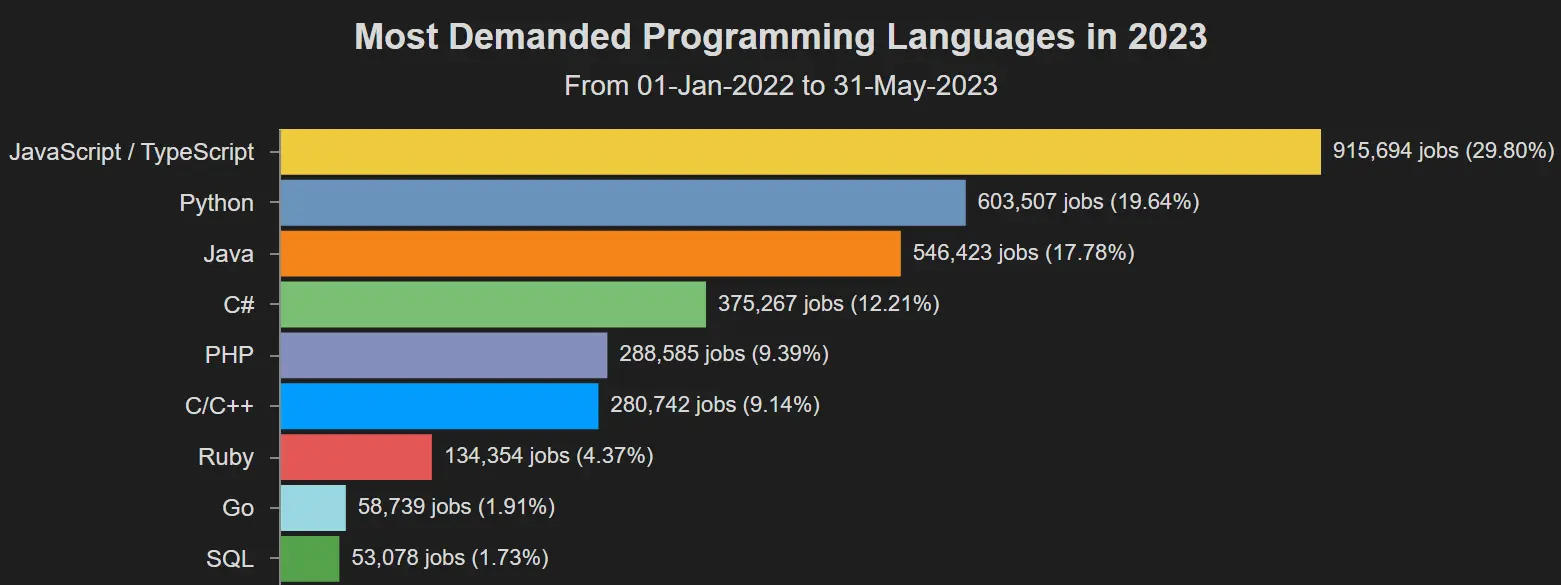
\includegraphics[keepaspectratio]{img/lenguajes.png}
  \caption{Lenguajes más demandados en 2023}
  \label{fig:lenguajesDemandados}
\end{figure}


\section{Lenguajes interpretados y compilados}\label{lenguajes-interpretados-y-compilados}

La principal diferencia entre los lenguajes de programación compilados y
los interpretados radica en cómo se ejecutan las instrucciones del
programa:

\subsection{Lenguajes de Programación Compilados}\label{lenguajes-de-programaciuxf3n-compilados}

\begin{enumerate}
  \item Proceso de Compilación: 
    \begin{itemize}
      \item
        Compilador: Un compilador traduce el código fuente completo a código
        máquina o bytecode antes de que el programa se ejecute. Este proceso
        se realiza una sola vez y genera un archivo ejecutable independiente.
      \item
        Ejemplo: C, C++, Rust, Go.
      \end{itemize}

  \item Ventajas:
      \begin{itemize}
        \item
          Rendimiento: Los programas compilados suelen ejecutarse más rápido que
          los interpretados porque la traducción a código máquina se realiza una
          sola vez y el ejecutable resultante está optimizado.
        \item
          Optimización: Los compiladores pueden realizar optimizaciones
          avanzadas durante la compilación para mejorar la eficiencia del
          programa.
      \end{itemize}

  \item Desventajas:
      \begin{itemize}
        \item
          Tiempo de Compilación: El proceso de compilación puede ser lento,
          especialmente para programas grandes.
        \item
          Portabilidad: El código compilado suele estar ligado a una plataforma
          específica, lo que puede dificultar su portabilidad a diferentes
          sistemas operativos.
      \end{itemize}
\end{enumerate}

\subsection{Lenguajes de Programación Interpretados}\label{lenguajes-de-programaciuxf3n-interpretados}

\begin{enumerate}
  \item Proceso de Interpretación:
    \begin{itemize}
      \item
        Intérprete: Un intérprete traduce y ejecuta el código fuente línea por
        línea en tiempo de ejecución, sin generar un archivo ejecutable
        intermedio.
      \item
        Ejemplo: Python, JavaScript, Ruby, PHP.
    \end{itemize}
  \item Ventajas:
    \begin{itemize}
      \item
        Desarrollo Rápido: No es necesario compilar el código antes de
        ejecutarlo, lo que permite ciclos de desarrollo y pruebas más rápidos.
      \item
        Portabilidad: Los programas interpretados pueden ejecutarse en
        cualquier plataforma que tenga el intérprete adecuado, lo que mejora
        su portabilidad.
    \end{itemize}

  \item Desventajas:
    \begin{itemize}
      \item
        Rendimiento: Los programas interpretados suelen ser más lentos que los
        compilados porque la traducción a código máquina ocurre en tiempo de
        ejecución.
      \item
        Optimización: Las oportunidades de optimización en tiempo de ejecución
        son limitadas en comparación con la compilación previa.
    \end{itemize}
  
\end{enumerate}


\subsection{Ejemplos y Consideraciones}\label{ejemplos-y-consideraciones}

\begin{description}
\item[Java:] Es un caso interesante porque utiliza un enfoque mixto. El
  código Java se compila en bytecode, que es interpretado por la Máquina
  Virtual de Java (JVM). Además, la JVM utiliza un compilador JIT
  (Just-In-Time) para convertir partes del bytecode en código máquina
  durante la ejecución, combinando ventajas de ambos enfoques.
\item[Python:] Aunque es principalmente un lenguaje interpretado, también
  puede ser compilado a bytecode (.pyc) para ser ejecutado por la
  máquina virtual de Python, lo que mejora ligeramente su rendimiento,
  pero no alcanza la velocidad de un lenguaje completamente compilado
  como C++.
\end{description}

En conclusión, la elección entre un lenguaje compilado y uno
interpretado depende de varios factores, incluyendo la necesidad de
rendimiento, la rapidez del desarrollo, y la portabilidad del código.

\section{Python}\label{python}

\subsection{¿Qué es Python?}\label{quuxe9-es-python}

Python es un lenguaje de programación popular. Fue creado por Guido van
Rossum y lanzado en 1991.

Se utiliza para:

\begin{itemize}
  \item Desarrollo web (del lado del servidor),
  \item Desarrollo de software,
  \item Matemáticas,
  \item Inteligencia Artificial,
  \item Scripting.
\end{itemize}

\subsection{¿Qué puede hacer Python?}\label{quuxe9-puede-hacer-python}

\begin{itemize}
  \item Python se puede utilizar en un servidor para crear aplicaciones web.
  \item Python se puede utilizar junto con el software para crear flujos de trabajo.
  \item Python puede conectarse a sistemas de bases de datos. También puede
    leer y modificar archivos.
  \item Python se puede utilizar para manejar Big Data y realizar matemáticas
    complejas.
  \item Python se puede utilizar para la creación rápida de prototipos o para
    el desarrollo de software listo para producción.
\end{itemize}

\subsection{¿Por qué Python?}\label{por-quuxe9-python}

\begin{itemize}
  \item Python funciona en diferentes plataformas (Windows, Mac, Linux,
    Raspberry Pi, etc.).
  \item Python tiene una sintaxis simple similar a la del idioma inglés.
  \item Python tiene una sintaxis que permite a los desarrolladores escribir
    programas con menos líneas que otros lenguajes de programación.
  \item Python se ejecuta en un sistema de interpretación, lo que significa
    que el código se puede ejecutar tan pronto como se escribe. Esto
    significa que la creación de prototipos puede ser muy rápida.
  \item Python se puede tratar de forma procedimental, orientada a objetos o
    funcional.
\end{itemize}

\subsection{Es bueno saber}\label{es-bueno-saber}

\begin{itemize}
\item
  La versión principal más reciente de Python es Python 3, que usaremos
  en este curso. Sin embargo, Python 2, aunque no se actualiza con nada
  más que actualizaciones de seguridad, sigue siendo bastante popular.
\item
  En este curso, Python se escribirá en un editor de texto. Es posible
  escribir Python en un entorno de desarrollo integrado, como Thonny,
  Pycharm, Visual Studio Code, Google Colaboratory, Netbeans o Eclipse,
  que son particularmente útiles cuando se administran colecciones más
  grandes de archivos Python.
\end{itemize}

\subsection{Sintaxis de Python comparada con otros lenguajes de
programación}\label{sintaxis-de-python-comparada-con-otros-lenguajes-de-programaciuxf3n}

\begin{itemize}
\item
  Python fue diseñado para facilitar la lectura y tiene algunas
  similitudes con el idioma inglés con influencia de las matemáticas.
\item
  Python usa nuevas líneas para completar un comando, a diferencia de
  otros lenguajes de programación que suelen usar punto y coma o
  paréntesis.
\item
  Python se basa en la sangría, utilizando espacios en blanco, para
  definir el alcance; como el alcance de los bucles, funciones y clases.
  Otros lenguajes de programación suelen utilizar llaves para este
  propósito.
\end{itemize}

\subsection{Instalación de Python}\label{instalaciuxf3n-de-python}

Muchas PC y Mac ya tienen Python instalado.

Para comprobar si tiene Python instalado en una PC con Windows, busque
Python en la barra de inicio o ejecute lo siguiente en la línea de
comandos (cmd.exe):

\begin{verbatim}
C:\Usuarios\Su nombre>python --version
\end{verbatim}

Para verificar si tiene Python instalado en Linux o Mac, en Linux abra
la línea de comando o en Mac abra la Terminal y escriba:

\begin{verbatim}
python --versión
\end{verbatim}

Si descubre que no tiene Python instalado en su computadora, puede
descargarlo de forma gratuita desde el siguiente sitio web:
\url{https://www.python.org/}

\subsection{Mi primer programa en Python}\label{mi-primer-programa-en-python}

\begin{Shaded}
\begin{Highlighting}[]
\BuiltInTok{print}\NormalTok{(}\StringTok{"Hola mundo"}\NormalTok{)}
\end{Highlighting}
\end{Shaded}

\section{Funciones}\label{funciones}

Una función es un bloque de código que sólo se ejecuta cuando se llama.
Puede pasar datos, conocidos como parámetros, a una función. Una función
puede devolver datos como resultado.

\subsection{Declarar una función}\label{declarar-una-funciuxf3n}

En Python una función se define usando la palabra clave \texttt{def}:

\begin{Shaded}
\begin{Highlighting}[]
\KeywordTok{def}\NormalTok{ mi\_función():}
    \BuiltInTok{print}\NormalTok{(}\StringTok{"Hola desde una función"}\NormalTok{)}
\end{Highlighting}
\end{Shaded}

\subsection{Llamar a una función}\label{llamar-a-una-funciuxf3n}

Para llamar a una función, use el nombre de la función seguido de
paréntesis:

\begin{Shaded}
\begin{Highlighting}[]
\KeywordTok{def}\NormalTok{ mi\_función():}
    \BuiltInTok{print}\NormalTok{(}\StringTok{"Hola desde una función"}\NormalTok{)}

\NormalTok{mi\_función()}
\end{Highlighting}
\end{Shaded}

\subsection{Argumentos}\label{argumentos}

La información se puede pasar a funciones como argumentos. Los
argumentos se especifican después del nombre de la función, dentro del
paréntesis. Puedes agregar tantos argumentos como quieras, simplemente
sepáralos con una coma.

El siguiente ejemplo tiene una función con un argumento (fname). Cuando
se llama a la función, pasamos un nombre, que se usa dentro de la
función para imprimir el nombre completo:

\begin{Shaded}
\begin{Highlighting}[]
\KeywordTok{def}\NormalTok{ mi\_función(fname):}
    \BuiltInTok{print}\NormalTok{(fnombre }\OperatorTok{+} \StringTok{" Refsnes"}\NormalTok{)}

\NormalTok{mi\_funcion(}\StringTok{"Emil"}\NormalTok{)}
\NormalTok{mi\_función(}\StringTok{"Tobías"}\NormalTok{)}
\NormalTok{mi\_función(}\StringTok{"Linus"}\NormalTok{)}
\end{Highlighting}
\end{Shaded}

\subsection{Argumentos arbitrarios,
*args}\label{argumentos-arbitrarios-args}

Si no sabe cuántos argumentos se pasarán a su función, agregue un
\_\_*\_\_ antes del nombre del parámetro en la definición de la función.
De esta manera, la función recibirá una tupla de argumentos y podrá
acceder a los elementos en consecuencia:

\begin{Shaded}
\begin{Highlighting}[]
\KeywordTok{def}\NormalTok{ mi\_funcion(}\OperatorTok{*}\NormalTok{ninos):}
    \BuiltInTok{print}\NormalTok{(}\StringTok{"El hijo menor es "} \OperatorTok{+}\NormalTok{ ninos[}\DecValTok{2}\NormalTok{])}

\NormalTok{mi\_funcion(}\StringTok{"Emil"}\NormalTok{, }\StringTok{"Tobías"}\NormalTok{, }\StringTok{"Linus"}\NormalTok{)}
\end{Highlighting}
\end{Shaded}

\section{Módulos de Python}\label{muxf3dulos-de-python}

\subsection{¿Qué es un módulo?}\label{quuxe9-es-un-muxf3dulo}

Considere que un módulo es lo mismo que una biblioteca de código. Un
archivo que contiene un conjunto de funciones que desea incluir en su
aplicación.

\subsection{Crear un módulo}\label{crear-un-muxf3dulo}

Para crear un módulo simplemente guarde el código que desea en un
archivo con la extensión de archivo \texttt{.py}:

\textbf{Ejemplo} Guarde este código en un archivo
\texttt{llamadomymodule.py}

\begin{Shaded}
\begin{Highlighting}[]
\KeywordTok{def}\NormalTok{ greeting(name):}
    \BuiltInTok{print}\NormalTok{(}\StringTok{"Hello, "} \OperatorTok{+}\NormalTok{ name)}
\end{Highlighting}
\end{Shaded}

\subsection{Utilice un módulo}\label{utilice-un-muxf3dulo}

Ahora podemos utilizar el módulo que acabamos de crear, mediante la
importdeclaración: \textbf{Ejemplo} Importa el módulo llamado mymodule y
llama a la función de saludo:

\begin{Shaded}
\begin{Highlighting}[]
    \ImportTok{import}\NormalTok{ mymodule}

\NormalTok{    mymodule.greeting(}\StringTok{"Jonathan"}\NormalTok{)}
\end{Highlighting}
\end{Shaded}

\subsection{Variables en el módulo}\label{variables-en-el-muxf3dulo}

El módulo puede contener funciones, como ya se ha descrito, pero también
variables de todo tipo (matrices, diccionarios, objetos, etc.):

\textbf{Ejemplo} Guarda este código en el \texttt{archivomymodule.py}

\begin{Shaded}
\begin{Highlighting}[]
\NormalTok{person1 }\OperatorTok{=}\NormalTok{ \{}
    \StringTok{"name"}\NormalTok{: }\StringTok{"John"}\NormalTok{,}
    \StringTok{"age"}\NormalTok{: }\DecValTok{36}\NormalTok{,}
    \StringTok{"country"}\NormalTok{: }\StringTok{"Norway"}
\NormalTok{\}}
\end{Highlighting}
\end{Shaded}

\textbf{Ejemplo} Importe el módulo llamado \texttt{mymodule} y acceda al
diccionario \texttt{person1}:

\begin{Shaded}
\begin{Highlighting}[]
    \ImportTok{import}\NormalTok{ mymodule}

\NormalTok{    a }\OperatorTok{=}\NormalTok{ mymodule.person1[}\StringTok{"age"}\NormalTok{]}
    \BuiltInTok{print}\NormalTok{(a)}
\end{Highlighting}
\end{Shaded}

\subsection{Nombrar un módulo}\label{nombrar-un-muxf3dulo}

Puedes nombrar el archivo del módulo como quieras, pero debe tener la
extensión de archivo \texttt{.py}

\subsection{Cambiar el nombre de un
módulo}\label{cambiar-el-nombre-de-un-muxf3dulo}

Puedes crear un alias al importar un módulo, utilizando la aspalabra
clave:

\textbf{Ejemplo} Crear un alias para mymoduleel llamado \texttt{mx}:

\begin{Shaded}
\begin{Highlighting}[]
\ImportTok{import}\NormalTok{ mymodule }\ImportTok{as}\NormalTok{ mx}

\NormalTok{a }\OperatorTok{=}\NormalTok{ mx.person1[}\StringTok{"age"}\NormalTok{]}
\BuiltInTok{print}\NormalTok{(a)}
\end{Highlighting}
\end{Shaded}

\subsection{Módulos integrados}\label{muxf3dulos-integrados}

Hay varios módulos integrados en Python que puedes importar cuando
quieras.

\textbf{Ejemplo} Importar y utilizar el \texttt{platformmódulo}:

\begin{Shaded}
\begin{Highlighting}[]
\ImportTok{import}\NormalTok{ platform}

\NormalTok{x }\OperatorTok{=}\NormalTok{ platform.system()}
\BuiltInTok{print}\NormalTok{(x)}
\end{Highlighting}
\end{Shaded}

\subsection{Usando la función dir()}\label{usando-la-funciuxf3n-dir}

Hay una función incorporada para enumerar todos los nombres de funciones
(o nombres de variables) en un módulo. La función \texttt{dir()}:

\textbf{Ejemplo} Enumere todos los nombres definidos que pertenecen al
módulo de la plataforma:

\begin{Shaded}
\begin{Highlighting}[]
\ImportTok{import}\NormalTok{ platform}

\NormalTok{x }\OperatorTok{=} \BuiltInTok{dir}\NormalTok{(platform)}
\BuiltInTok{print}\NormalTok{(x)}
\end{Highlighting}
\end{Shaded}

\subsection{Importar desde módulo}\label{importar-desde-muxf3dulo}

Puede elegir importar solo partes de un módulo, utilizando la
frompalabra clave.

\textbf{Ejemplo} El módulo nombrado \texttt{mymodule} tiene una función
y un diccionario:

\begin{Shaded}
\begin{Highlighting}[]
\KeywordTok{def}\NormalTok{ greeting(name):}
    \BuiltInTok{print}\NormalTok{(}\StringTok{"Hello, "} \OperatorTok{+}\NormalTok{ name)}

\NormalTok{person1 }\OperatorTok{=}\NormalTok{ \{}
    \StringTok{"name"}\NormalTok{: }\StringTok{"John"}\NormalTok{,}
    \StringTok{"age"}\NormalTok{: }\DecValTok{36}\NormalTok{,}
    \StringTok{"country"}\NormalTok{: }\StringTok{"Norway"}
\NormalTok{\}}
\end{Highlighting}
\end{Shaded}

\textbf{Ejemplo} Importe únicamente el diccionario \texttt{person1} del
módulo:

\begin{Shaded}
\begin{Highlighting}[]
\ImportTok{from}\NormalTok{ mymodule }\ImportTok{import}\NormalTok{ person1}

\BuiltInTok{print}\NormalTok{ (person1[}\StringTok{"age"}\NormalTok{])}
\end{Highlighting}
\end{Shaded}

\section{Referencias}

\begin{itemize}
\tightlist
\item
  \href{https://www.w3schools.com/python/}{Python en la W3Schools}
\item
  \href{https://www.python.org/}{Python.org}
\item
  \href{https://chatgpt.com/}{chatGPT en openAI}
\item
  \href{https://lab.anahuac.mx/~hselley/ayp/conceptosBasicos.html}{Algoritmos
  y Programación}
\item
  \href{https://lab.anahuac.mx/~hselley/mn/python.html}{Sintaxis básica
  en Python}
\end{itemize}


    % Chapter 2
    \chapter{Sintáxis Básica de Python}
\section{Python}

\href{https://www.python.org/about/}{Python} es un lenguaje de
programación poderoso y rápido, se lleva bien con otros lenguajes, corre
en cualquier lugar, es amigable, fácil de aprender y es de software
libre.

\section{Sintáxis}

En la gran mayoría de los lenguajes de programación el compilador o
intérprete ignora los espacios que el usuario utilice para escribir su
código. En Python, los espacios se utilizan para formar grupos de
instrucciones y también para la sintaxis de algunas instrucciones.

\section{If-Elif-Else}

La sentencia de control \texttt{if-elif-else} tiene la siguiente
sintaxis:

Sintaxis:

\begin{Shaded}
\begin{Highlighting}[]
\ControlFlowTok{if}\NormalTok{ condición A:}
\NormalTok{    instrucción A1}
\NormalTok{    instrucción A2}
\NormalTok{    ...}
\NormalTok{    instrucción An}
\ControlFlowTok{elif}\NormalTok{ condición B:}
\NormalTok{    instrucción B1}
\NormalTok{    instrucción B2}
\NormalTok{    ...}
\NormalTok{    instrucción Bn}
\ControlFlowTok{else}\NormalTok{:}
\NormalTok{    instrucción C1}
\NormalTok{    instrucción C2}
\NormalTok{    ...}
\NormalTok{    instrucción Cn}

\end{Highlighting}
\end{Shaded}


\begin{code} if-else
\begin{Shaded}
\begin{Highlighting}[]
    \ControlFlowTok{if} \DecValTok{2}\OperatorTok{\textless{}}\DecValTok{3}\NormalTok{:}
        \BuiltInTok{print}\NormalTok{(}\StringTok{"verdadero"}\NormalTok{)}
    \ControlFlowTok{else}\NormalTok{:}
        \BuiltInTok{print}\NormalTok{(}\StringTok{"falso"}\NormalTok{)}
    \BuiltInTok{print}\NormalTok{(}\StringTok{"fin"}\NormalTok{)}

\end{Highlighting}
\end{Shaded}
\end{code}

\begin{code}
Solicite dos números x y \texttt{y}. Si \texttt{x}
es positivo \texttt{y} se multiplica por dos, si \texttt{x} es cero
\texttt{y} se multiplica por 3 y si \texttt{x} es negativo y se
multiplica por cuatro.

\begin{Shaded}
\begin{Highlighting}[]
\NormalTok{    x}\OperatorTok{=}\BuiltInTok{int}\NormalTok{(}\BuiltInTok{input}\NormalTok{(}\StringTok{"Ingrese el valor de x "}\NormalTok{))}
\NormalTok{    y}\OperatorTok{=}\BuiltInTok{int}\NormalTok{(}\BuiltInTok{input}\NormalTok{(}\StringTok{"Ingrese el valor de y "}\NormalTok{))}
    \ControlFlowTok{if}\NormalTok{ x}\OperatorTok{\textgreater{}}\DecValTok{0}\NormalTok{:}
\NormalTok{        z}\OperatorTok{=}\NormalTok{y}\OperatorTok{*}\DecValTok{2}
        \BuiltInTok{print}\NormalTok{(}\StringTok{"Positivo"}\NormalTok{)}
    \ControlFlowTok{elif}\NormalTok{ x}\OperatorTok{==}\DecValTok{0}\NormalTok{:}
\NormalTok{        z}\OperatorTok{=}\NormalTok{y}\OperatorTok{*}\DecValTok{3}
        \BuiltInTok{print}\NormalTok{(}\StringTok{"Cero"}\NormalTok{)}
    \ControlFlowTok{else}\NormalTok{:}
\NormalTok{        z}\OperatorTok{=}\NormalTok{y}\OperatorTok{*}\DecValTok{4}
        \BuiltInTok{print}\NormalTok{(}\StringTok{"Negativo"}\NormalTok{)}
    \BuiltInTok{print}\NormalTok{(z)}
\end{Highlighting}
\end{Shaded}
\end{code}

\section{For}

El ciclo \texttt{for} tiene la siguiente sintaxis:

\begin{Shaded}
\begin{Highlighting}[]
\ControlFlowTok{for}\NormalTok{ iterador }\KeywordTok{in}\NormalTok{ iterando:}
\NormalTok{    instrucción }\DecValTok{1}
\NormalTok{    instrucción }\DecValTok{2}
\NormalTok{    ...}
\NormalTok{    instrucción n}

\end{Highlighting}
\end{Shaded}

\begin{code} Un ciclo que imprime numeros enteros desde 0 hasta 9.

\begin{Shaded}
\begin{Highlighting}[]
\ControlFlowTok{for}\NormalTok{ i }\KeywordTok{in} \BuiltInTok{range}\NormalTok{(}\DecValTok{10}\NormalTok{):}
    \BuiltInTok{print}\NormalTok{(i)}
\end{Highlighting}
\end{Shaded}
    
\end{code}
 

La función \texttt{range} genera una secuencia de números enteros
comenzando desde 0, con un incremento unitario. Por esa razón es que se
generan los números enteros desde 0 hasta 9. Es posible cambiar el valor
inicial de la secuencia y el incremento.

\begin{code} Considere los primeros 10 números naturales, los
pimeros 5 urales se multiplican por 2 y los siguientes números naturales
se multiplican por 3.

\begin{Shaded}
\begin{Highlighting}[]
    \ControlFlowTok{for}\NormalTok{ x }\KeywordTok{in} \BuiltInTok{range}\NormalTok{(}\DecValTok{1}\NormalTok{,}\DecValTok{11}\NormalTok{):}
        \ControlFlowTok{if}\NormalTok{ x}\OperatorTok{\textless{}=}\DecValTok{5}\NormalTok{:}
            \BuiltInTok{print}\NormalTok{(}\SpecialStringTok{f\textquotesingle{}}\SpecialCharTok{\{}\NormalTok{x}\SpecialCharTok{\}}\SpecialStringTok{ {-}\textgreater{} }\SpecialCharTok{\{}\NormalTok{x}\OperatorTok{*}\DecValTok{2}\SpecialCharTok{\}}\SpecialStringTok{\textquotesingle{}}\NormalTok{)}
        \ControlFlowTok{else}\NormalTok{:}
            \BuiltInTok{print}\NormalTok{(}\SpecialStringTok{f\textquotesingle{}}\SpecialCharTok{\{}\NormalTok{x}\SpecialCharTok{\}}\SpecialStringTok{ {-}\textgreater{} }\SpecialCharTok{\{}\NormalTok{x}\OperatorTok{*}\DecValTok{3}\SpecialCharTok{\}}\SpecialStringTok{\textquotesingle{}}\NormalTok{)}
\end{Highlighting}
\end{Shaded}
\end{code}

\section{While} 
El ciclo \texttt{while} repite las instrucciones siempre y cuando la
condición sea verdadera. La sintaxis del ciclo \texttt{while} es la
siguiente:

\begin{Shaded}
\begin{Highlighting}[]
    \ControlFlowTok{while}\NormalTok{ condición:}
\NormalTok{        instrucción }\DecValTok{1}
\NormalTok{        instrucción }\DecValTok{2}
\NormalTok{        ...}
\NormalTok{        instrucción n}

\end{Highlighting}
\end{Shaded}

\begin{code} Se imprimen los primeros 10 numeros naturales.

\begin{Shaded}
\begin{Highlighting}[]
\NormalTok{    i }\OperatorTok{=} \DecValTok{1}
    \ControlFlowTok{while}\NormalTok{ i }\OperatorTok{\textless{}=} \DecValTok{10}\NormalTok{:}
        \BuiltInTok{print}\NormalTok{(i)}
\NormalTok{        i}\OperatorTok{=}\NormalTok{i}\OperatorTok{+}\DecValTok{1}
\end{Highlighting}
\end{Shaded}
\end{code}

\section{Listas}

\subsection{Creación}

Una lista es un conjunto de valores ordenados y modificables que permite
repeticiones. Los elementos en la lista son numerados comenzando desde
0, de manera que la localidad donde se encuentra el último elemento para
una lista de tamaño \texttt{n} será \texttt{n-1}.

\begin{Shaded}
\begin{Highlighting}[]
\NormalTok{    lista }\OperatorTok{=}\NormalTok{ [}\StringTok{"manzana"}\NormalTok{, }\StringTok{"plátano"}\NormalTok{, }\StringTok{"naranja"}\NormalTok{, }\StringTok{"mandarina"}\NormalTok{, }\StringTok{"maracuyá"}\NormalTok{]}
    \BuiltInTok{print}\NormalTok{(lista)}
\end{Highlighting}
\end{Shaded}

\subsection{Acceso}

El acceso a algún elemento en particular de la lista se hace utilizando
los corchetes, indicando dentro de ellos la posición que ocupa dentro de
la lista.

\begin{Shaded}
\begin{Highlighting}[]
\NormalTok{    lista[posición]}
\end{Highlighting}
\end{Shaded}

\subsection{Índices negativos}

Es posible usar numeración negativa para hacer referencia a los
elementos dentro de una lista pero en orden reverso. Es decir,
\texttt{-1} hace referencia al último elemento, \texttt{-2} al
penúltimo, \texttt{-3} al antepenúltimo y así sucesivamente.

\subsection{Rango de índices}

Es posible seleccionar un subconjunto de elementos contiguos contenidos
en la lista especificando el rango de posiciones que ocupan dentro de la
lista.

\begin{Shaded}
\begin{Highlighting}[]
\NormalTok{    lista }\OperatorTok{=}\NormalTok{ [}\StringTok{"manzana"}\NormalTok{, }\StringTok{"plátano"}\NormalTok{, }\StringTok{"naranja"}\NormalTok{, }\StringTok{"mandarina"}\NormalTok{, }\StringTok{"maracuyá"}\NormalTok{, }
            \StringTok{"toronja"}\NormalTok{, }\StringTok{"mango"}\NormalTok{, }\StringTok{"guayaba"}\NormalTok{]}
    \BuiltInTok{print}\NormalTok{(lista[}\DecValTok{2}\NormalTok{:}\DecValTok{6}\NormalTok{])}
\end{Highlighting}
\end{Shaded}

Por otro lado, si se omite el límite inferior del rango, python
considerará 0 como posición inicial.

\begin{Shaded}
\begin{Highlighting}[]
\NormalTok{    lista }\OperatorTok{=}\NormalTok{ [}\StringTok{"manzana"}\NormalTok{, }\StringTok{"plátano"}\NormalTok{, }\StringTok{"naranja"}\NormalTok{, }\StringTok{"mandarina"}\NormalTok{, }\StringTok{"maracuyá"}\NormalTok{, }
            \StringTok{"toronja"}\NormalTok{, }\StringTok{"mango"}\NormalTok{, }\StringTok{"guayaba"}\NormalTok{]}
    \BuiltInTok{print}\NormalTok{(lista[:}\DecValTok{6}\NormalTok{])}
\end{Highlighting}
\end{Shaded}

Finalmente, si se omite el límite superior del rango, python considerará
el último elemento como tal límite.

\begin{Shaded}
\begin{Highlighting}[]
\NormalTok{    lista }\OperatorTok{=}\NormalTok{ [}\StringTok{"manzana"}\NormalTok{, }\StringTok{"plátano"}\NormalTok{, }\StringTok{"naranja"}\NormalTok{, }\StringTok{"mandarina"}\NormalTok{, }\StringTok{"maracuyá"}\NormalTok{, }
            \StringTok{"toronja"}\NormalTok{, }\StringTok{"mango"}\NormalTok{, }\StringTok{"guayaba"}\NormalTok{]}
    \BuiltInTok{print}\NormalTok{(lista[}\DecValTok{2}\NormalTok{:])}
\end{Highlighting}
\end{Shaded}

\subsection{Tamaño de una lista}

Para determinar el tamaño de una lista se puede utilizar la función
\texttt{len()}

\begin{Shaded}
\begin{Highlighting}[]
    \BuiltInTok{print}\NormalTok{(}\BuiltInTok{len}\NormalTok{(lista))}
\end{Highlighting}
\end{Shaded}

\section{Funciones}

En python la declaración de funciones requiere muy poco código. Basta
con utilizar la palabra clave \texttt{def} para comenzar la definición
de la función.

\begin{Shaded}
\begin{Highlighting}[]
    \KeywordTok{def}\NormalTok{ nombreFuncion(parámetroEntrada):}
\NormalTok{        instrucción }\DecValTok{1}
\NormalTok{        instrucción }\DecValTok{2}
\NormalTok{        ...}
\NormalTok{        instrucción n}
        \ControlFlowTok{return}\NormalTok{ parámetroSalida}

\end{Highlighting}
\end{Shaded}

\begin{code} Escriba una función que calcule el factorial de una
función. Verifique que el número ingresado por el usuario sea positivo y
considere que por definición el factorial de cero es uno.

\begin{Shaded}
\begin{Highlighting}[]
    \KeywordTok{def}\NormalTok{ factorial(x):}
        \ControlFlowTok{if}\NormalTok{ x}\OperatorTok{\textgreater{}=}\DecValTok{0}\NormalTok{:}
\NormalTok{            f}\OperatorTok{=}\DecValTok{1}
        \ControlFlowTok{if}\NormalTok{ x}\OperatorTok{\textgreater{}}\DecValTok{0}\NormalTok{:}
\NormalTok{            f}\OperatorTok{=}\DecValTok{1}
            \ControlFlowTok{for}\NormalTok{ i }\KeywordTok{in} \BuiltInTok{range}\NormalTok{(}\DecValTok{1}\NormalTok{,x}\OperatorTok{+}\DecValTok{1}\NormalTok{):}
\NormalTok{            f}\OperatorTok{=}\NormalTok{f}\OperatorTok{*}\NormalTok{i}
            \ControlFlowTok{return}\NormalTok{ f}
        \ControlFlowTok{else}\NormalTok{:}
            \BuiltInTok{print}\NormalTok{(}\StringTok{"El factorial no está definido"}\NormalTok{)}

\NormalTok{    x }\OperatorTok{=} \BuiltInTok{int}\NormalTok{(}\BuiltInTok{input}\NormalTok{(}\StringTok{"Introduzca un número: "}\NormalTok{))}
    \BuiltInTok{print}\NormalTok{(}\SpecialStringTok{f\textquotesingle{}}\SpecialCharTok{\{}\NormalTok{x}\SpecialCharTok{\}}\SpecialStringTok{! = }\SpecialCharTok{\{}\NormalTok{factorial(x)}\SpecialCharTok{\}}\SpecialStringTok{\textquotesingle{}}\NormalTok{)      }

\end{Highlighting}
\end{Shaded}
\end{code}

\begin{code} Escriba una función que calcule el factorial de una
función. Considere la definción recursiva del factorial. Verifique que
el número ingresado por el usuario sea positivo y considere que por
definición el factorial de cero es uno.

\begin{Shaded}
\begin{Highlighting}[]
    \KeywordTok{def}\NormalTok{ factorial(x):}
        \ControlFlowTok{if}\NormalTok{ x}\OperatorTok{==}\DecValTok{0}\NormalTok{:}
\NormalTok{            f}\OperatorTok{=}\DecValTok{1}
        \ControlFlowTok{else}\NormalTok{:}
\NormalTok{            f}\OperatorTok{=}\NormalTok{x}\OperatorTok{*}\NormalTok{factorial(x}\OperatorTok{{-}}\DecValTok{1}\NormalTok{)}
        \ControlFlowTok{return}\NormalTok{(f)}

\NormalTok{    x }\OperatorTok{=} \BuiltInTok{int}\NormalTok{(}\BuiltInTok{input}\NormalTok{(}\StringTok{"Ingrese un número"}\NormalTok{))}
    \ControlFlowTok{if}\NormalTok{ x}\OperatorTok{\textgreater{}=}\DecValTok{0}\NormalTok{:}
\NormalTok{        fac}\OperatorTok{=}\NormalTok{factorial(x)}
        \BuiltInTok{print}\NormalTok{(}\SpecialStringTok{f\textquotesingle{}}\SpecialCharTok{\{}\NormalTok{x}\SpecialCharTok{\}}\SpecialStringTok{! = }\SpecialCharTok{\{}\NormalTok{fac}\SpecialCharTok{\}}\SpecialStringTok{\textquotesingle{}}\NormalTok{)}
    \ControlFlowTok{else}\NormalTok{:}
        \BuiltInTok{print}\NormalTok{(}\StringTok{"El factorial no está definido en los negativos"}\NormalTok{)    }

\end{Highlighting}
\end{Shaded}
\end{code}

\begin{code} Escriba una función recursiva que imprima los elementos de una lista anidada en varios niveles.

\begin{Shaded}
\begin{Highlighting}[]
\NormalTok{    lista1 }\OperatorTok{=}\NormalTok{ [}\StringTok{"manzana"}\NormalTok{, }\StringTok{"plátano"}\NormalTok{, }\StringTok{"naranja"}\NormalTok{, }\StringTok{"mandarina"}\NormalTok{, }\StringTok{"maracuyá"}\NormalTok{, }\StringTok{"toronja"}\NormalTok{, }
            \StringTok{"mango"}\NormalTok{, }\StringTok{"guayaba"}\NormalTok{]}
\NormalTok{    lista2 }\OperatorTok{=}\NormalTok{ [}\DecValTok{1}\NormalTok{, }\DecValTok{2}\NormalTok{, }\DecValTok{3}\NormalTok{, }\DecValTok{4}\NormalTok{, }\DecValTok{5}\NormalTok{]}
\NormalTok{    lista3 }\OperatorTok{=}\NormalTok{ [}\StringTok{"A"}\NormalTok{, }\StringTok{"B"}\NormalTok{, }\StringTok{"C"}\NormalTok{, }\StringTok{"D"}\NormalTok{]}
\NormalTok{    lista4 }\OperatorTok{=}\NormalTok{ [}\StringTok{"a"}\NormalTok{, }\DecValTok{1}\NormalTok{, }\StringTok{"b"}\NormalTok{, }\DecValTok{2}\NormalTok{, }\StringTok{"c"}\NormalTok{, }\DecValTok{3}\NormalTok{, }\StringTok{"d"}\NormalTok{, }\DecValTok{4}\NormalTok{]}
\NormalTok{    superLista }\OperatorTok{=}\NormalTok{ [lista1 }\OperatorTok{+}\NormalTok{ lista2 }\OperatorTok{+}\NormalTok{ lista3] }\OperatorTok{+}\NormalTok{ [[lista4]] }\OperatorTok{+}\NormalTok{ lista1}

    \KeywordTok{def}\NormalTok{ impresionRecursiva(listaAnidada):}
    \ControlFlowTok{for}\NormalTok{ elemento }\KeywordTok{in}\NormalTok{ listaAnidada:}
        \ControlFlowTok{if} \BuiltInTok{isinstance}\NormalTok{(elemento, }\BuiltInTok{list}\NormalTok{):}
\NormalTok{            impresionRecursiva(elemento)}
        \ControlFlowTok{else}\NormalTok{: }
            \BuiltInTok{print}\NormalTok{(elemento)}

\NormalTok{    impresionRecursiva(superLista)}
\end{Highlighting}
\end{Shaded}
\end{code}

\section{Arreglos}

Python no tiene de forma nativa soporte para arreglos, en su lugar opta
por usar listas anidadas. Sin embargo, es posible utilizar el paquete
\href{https://numpy.org/}{NumPy} para utilizar los arreglos de manera
semejante a la existente en otros lenguajes. \textbf{NumPy} además
resulta ser más eficiente en el manejo de datos que su contraparte
nativa de python mediante listas anidadas. Adicionalmente,
\textbf{NumPy} incluye más herramientas que extienden la funcionalidad
de Python.

\subsection{Declaración}

Sintaxis:

\begin{Shaded}
\begin{Highlighting}[]
    \ImportTok{import}\NormalTok{ numpy}
\NormalTok{    arreglo }\OperatorTok{=}\NormalTok{ numpy.array([}\DecValTok{1}\NormalTok{, }\DecValTok{2}\NormalTok{, }\DecValTok{3}\NormalTok{, }\DecValTok{4}\NormalTok{, }\DecValTok{5}\NormalTok{])}
    \BuiltInTok{print}\NormalTok{(arreglo)}
\end{Highlighting}
\end{Shaded}

Esta sintaxis puede resultar incómoda porque será necesario escribirla
todas las veces que necesite declarar un arreglo. Una alternativa para
simplificar un poco esta declaración es mediante la creación de un
alias, esto de la siguiente manera:

\begin{Shaded}
\begin{Highlighting}[]
    \ImportTok{import}\NormalTok{ numpy }\ImportTok{as}\NormalTok{ np}
\NormalTok{    arreglo }\OperatorTok{=}\NormalTok{ np.array([}\DecValTok{1}\NormalTok{, }\DecValTok{2}\NormalTok{, }\DecValTok{3}\NormalTok{, }\DecValTok{4}\NormalTok{, }\DecValTok{5}\NormalTok{])}
    \BuiltInTok{print}\NormalTok{(arreglo)}
\end{Highlighting}
\end{Shaded}

Para declarar un arreglo bidimensional se utiliza la siguiente sintáxis:

\begin{Shaded}
\begin{Highlighting}[]
    \ImportTok{import}\NormalTok{ numpy }\ImportTok{as}\NormalTok{ np}
\NormalTok{    arreglo }\OperatorTok{=}\NormalTok{ np.array([[}\DecValTok{1}\NormalTok{, }\DecValTok{2}\NormalTok{, }\DecValTok{3}\NormalTok{], [}\DecValTok{4}\NormalTok{, }\DecValTok{5}\NormalTok{, }\DecValTok{6}\NormalTok{]])}
    \BuiltInTok{print}\NormalTok{(arreglo) }
\end{Highlighting}
\end{Shaded}

El atributo \texttt{ndim} devuelve la cantidad de dimensiones que tiene
un arreglo.

\begin{Shaded}
\begin{Highlighting}[]
    \ImportTok{import}\NormalTok{ numpy }\ImportTok{as}\NormalTok{ np}
\NormalTok{    arreglo }\OperatorTok{=}\NormalTok{ np.array([[}\DecValTok{1}\NormalTok{, }\DecValTok{2}\NormalTok{, }\DecValTok{3}\NormalTok{], [}\DecValTok{4}\NormalTok{, }\DecValTok{5}\NormalTok{, }\DecValTok{6}\NormalTok{]])}
    \BuiltInTok{print}\NormalTok{(arreglo.ndim) }
\end{Highlighting}
\end{Shaded}

\subsection{Acceso a elementos de un arreglo}

El acceso a elementos dentro de un arreglo en \texttt{numpy} es similar
a la forma que se utiliza para las listas. Recuerde que elos índice para
los elementos dentro del arreglo comienza en 0.

\begin{Shaded}
\begin{Highlighting}[]
    \ImportTok{import}\NormalTok{ numpy }\ImportTok{as}\NormalTok{ np}
\NormalTok{    arreglo }\OperatorTok{=}\NormalTok{ np.array([}\DecValTok{1}\NormalTok{, }\DecValTok{2}\NormalTok{, }\DecValTok{3}\NormalTok{, }\DecValTok{4}\NormalTok{, }\DecValTok{5}\NormalTok{])}
    \BuiltInTok{print}\NormalTok{(arreglo[}\DecValTok{0}\NormalTok{])}
\end{Highlighting}
\end{Shaded}

Para el caso de un arreglo bidimensional se utiliza una coma para separar la posición de las dimensiones.

\begin{Shaded}
\begin{Highlighting}[]
    \ImportTok{import}\NormalTok{ numpy }\ImportTok{as}\NormalTok{ np}
\NormalTok{    arreglo }\OperatorTok{=}\NormalTok{ np.array([[}\DecValTok{1}\NormalTok{, }\DecValTok{2}\NormalTok{, }\DecValTok{3}\NormalTok{], [}\DecValTok{4}\NormalTok{, }\DecValTok{5}\NormalTok{, }\DecValTok{6}\NormalTok{]])}
    \BuiltInTok{print}\NormalTok{(arreglo[}\DecValTok{1}\NormalTok{, }\DecValTok{2}\NormalTok{]) }
\end{Highlighting}
\end{Shaded}

Si el arreglo tiene más dimensiones se utiliza la misma idea para cada una de ellas.

\begin{Shaded}
\begin{Highlighting}[]
    \ImportTok{import}\NormalTok{ numpy }\ImportTok{as}\NormalTok{ np}
\NormalTok{    arreglo }\OperatorTok{=}\NormalTok{ np.array([[[}\DecValTok{1}\NormalTok{, }\DecValTok{2}\NormalTok{, }\DecValTok{3}\NormalTok{], [}\DecValTok{4}\NormalTok{, }\DecValTok{5}\NormalTok{, }\DecValTok{6}\NormalTok{]],[[}\DecValTok{7}\NormalTok{, }\DecValTok{8}\NormalTok{, }\DecValTok{9}\NormalTok{], [}\DecValTok{10}\NormalTok{, }\DecValTok{11}\NormalTok{, }\DecValTok{12}\NormalTok{]])}
    \BuiltInTok{print}\NormalTok{(arreglo[}\DecValTok{0}\NormalTok{, }\DecValTok{1}\NormalTok{, }\DecValTok{2}\NormalTok{]) }
\end{Highlighting}
\end{Shaded}

De la misma forma que con las listas, también es posible utilizar índices negativos.

\begin{Shaded}
\begin{Highlighting}[]
\NormalTok{    arreglo }\OperatorTok{=}\NormalTok{ np.array([[}\DecValTok{1}\NormalTok{,}\DecValTok{2}\NormalTok{,}\DecValTok{3}\NormalTok{,}\DecValTok{4}\NormalTok{,}\DecValTok{5}\NormalTok{], [}\DecValTok{6}\NormalTok{,}\DecValTok{7}\NormalTok{,}\DecValTok{8}\NormalTok{,}\DecValTok{9}\NormalTok{,}\DecValTok{10}\NormalTok{]])}
    \BuiltInTok{print}\NormalTok{(}\StringTok{\textquotesingle{}El último elemento en el arreglo bidimensional\textquotesingle{}}\NormalTok{, arreglo[}\DecValTok{1}\NormalTok{, }\OperatorTok{{-}}\DecValTok{1}\NormalTok{]) }
\end{Highlighting}
\end{Shaded}

\subsection{Cortes de arreglos}

Es posible \emph{cortar} un subconjunto de un arreglo para definir uno
nuevo. Esto es de especial utilidad para extraer vectores de una matriz
existente, ya sea para definir un nuevo vector o bien realizar
operaciones con el.

El corte (o rebanada) de la matriz se hace indicando un rango de
posiciones, es decir \texttt{{[}inicio\ :\ fin{]}}. Además se puede
especificar un incremento \texttt{{[}inicio\ :\ fin\ :\ incremento{]}}.
Si no se especifica un inicio, de asume como 0, y si no se especifica un
final se asume el último elemento de la matriz. Si no se especifica un
incremento, se asume como 1.

\begin{Shaded}
\begin{Highlighting}[]
    \ImportTok{import}\NormalTok{ numpy }\ImportTok{as}\NormalTok{ np}
\NormalTok{    arreglo }\OperatorTok{=}\NormalTok{ np.array([}\DecValTok{1}\NormalTok{, }\DecValTok{2}\NormalTok{, }\DecValTok{3}\NormalTok{, }\DecValTok{4}\NormalTok{, }\DecValTok{5}\NormalTok{])}
\NormalTok{    arreglo2 }\OperatorTok{=}\NormalTok{ arreglo[}\DecValTok{1}\NormalTok{:}\DecValTok{4}\NormalTok{]}
    \BuiltInTok{print}\NormalTok{(arreglo2)}
\end{Highlighting}
\end{Shaded}

En el siguiente ejemplo, se hace una rebanada de la matriz especificando
un incremento diferente a uno:

\begin{Shaded}
\begin{Highlighting}[]
    \ImportTok{import}\NormalTok{ numpy }\ImportTok{as}\NormalTok{ np}
\NormalTok{    arreglo }\OperatorTok{=}\NormalTok{ np.array([}\DecValTok{1}\NormalTok{, }\DecValTok{2}\NormalTok{, }\DecValTok{3}\NormalTok{, }\DecValTok{4}\NormalTok{, }\DecValTok{5}\NormalTok{, }\DecValTok{6}\NormalTok{, }\DecValTok{7}\NormalTok{])}
    \BuiltInTok{print}\NormalTok{(arreglo[}\DecValTok{1}\NormalTok{:}\DecValTok{5}\NormalTok{:}\DecValTok{2}\NormalTok{])}
\end{Highlighting}
\end{Shaded}

\subsection{Cortes de arreglos bidimensionales}

Es posible realizar rebanadas de arreglos de 2 ó más dimensiones,
resultando un vector o una matriz según sea el caso.

El siguiente ejemplo realiza una rebanada de un arreglo bidimensional y
el resultado es un vector. Observe que el vector es una rebanada de la
segunda dimensión de la matriz.

\begin{Shaded}
\begin{Highlighting}[]
    \ImportTok{import}\NormalTok{ numpy }\ImportTok{as}\NormalTok{ np}
\NormalTok{    arreglo }\OperatorTok{=}\NormalTok{ np.array([[}\DecValTok{1}\NormalTok{, }\DecValTok{2}\NormalTok{, }\DecValTok{3}\NormalTok{, }\DecValTok{4}\NormalTok{, }\DecValTok{5}\NormalTok{], [}\DecValTok{6}\NormalTok{, }\DecValTok{7}\NormalTok{, }\DecValTok{8}\NormalTok{, }\DecValTok{9}\NormalTok{, }\DecValTok{10}\NormalTok{]])}
    \BuiltInTok{print}\NormalTok{(arreglo[}\DecValTok{1}\NormalTok{, }\DecValTok{1}\NormalTok{:}\DecValTok{4}\NormalTok{])}
\end{Highlighting}
\end{Shaded}

En este ejemplo se hace una rebanada de un arreglo bidimensional y el
resultado es nuevamente un vector. En esta ocasión el vector es una
rebanada vertical por lo que el resultado contiene elementos de ambas
dimensiones de la matriz.

\begin{Shaded}
\begin{Highlighting}[]
    \ImportTok{import}\NormalTok{ numpy }\ImportTok{as}\NormalTok{ np}
\NormalTok{    arreglo }\OperatorTok{=}\NormalTok{ np.array([[}\DecValTok{1}\NormalTok{, }\DecValTok{2}\NormalTok{, }\DecValTok{3}\NormalTok{, }\DecValTok{4}\NormalTok{, }\DecValTok{5}\NormalTok{], [}\DecValTok{6}\NormalTok{, }\DecValTok{7}\NormalTok{, }\DecValTok{8}\NormalTok{, }\DecValTok{9}\NormalTok{, }\DecValTok{10}\NormalTok{]])}
    \BuiltInTok{print}\NormalTok{(arreglo[}\DecValTok{0}\NormalTok{:}\DecValTok{2}\NormalTok{, }\DecValTok{2}\NormalTok{])}
\end{Highlighting}
\end{Shaded}

En este último caso, se hace una rebanada que resulta una matriz que
contiene elementos de ambas dimensiones de la matriz original.

\begin{Shaded}
\begin{Highlighting}[]
    \ImportTok{import}\NormalTok{ numpy }\ImportTok{as}\NormalTok{ np}
\NormalTok{    arreglo }\OperatorTok{=}\NormalTok{ np.array([[}\DecValTok{1}\NormalTok{, }\DecValTok{2}\NormalTok{, }\DecValTok{3}\NormalTok{, }\DecValTok{4}\NormalTok{, }\DecValTok{5}\NormalTok{], [}\DecValTok{6}\NormalTok{, }\DecValTok{7}\NormalTok{, }\DecValTok{8}\NormalTok{, }\DecValTok{9}\NormalTok{, }\DecValTok{10}\NormalTok{]])}
    \BuiltInTok{print}\NormalTok{(arreglo[}\DecValTok{0}\NormalTok{:}\DecValTok{2}\NormalTok{, }\DecValTok{1}\NormalTok{:}\DecValTok{4}\NormalTok{])}
\end{Highlighting}
\end{Shaded}

\subsection{Arreglos aleatorios}

Es posible generar un arreglo o matriz lleno de números (pseudo)
aleatorios, para ello se puede utilizar el método \texttt{rand}. Para la
generación, basta con especificar las dimensiones del arreglo que se
desea generar.\\


\begin{code} Generación de un vector unidimensional de 20 elementos aleatorios.

\begin{Shaded}
\begin{Highlighting}[]
    \ImportTok{import}\NormalTok{ numpy }\ImportTok{as}\NormalTok{ np}
\NormalTok{    arreglo }\OperatorTok{=}\NormalTok{ np.random.rand(}\DecValTok{20}\NormalTok{) }
    \BuiltInTok{print}\NormalTok{(arreglo)}

\end{Highlighting}
\end{Shaded}
\end{code}

\begin{code} Generación de una matriz bidimensional de tamaño \texttt{5x3}, es decir 5 renglones y 3 columnas.

\begin{Shaded}
\begin{Highlighting}[]
    \ImportTok{import}\NormalTok{ numpy }\ImportTok{as}\NormalTok{ np}
\NormalTok{    arreglo }\OperatorTok{=}\NormalTok{ np.random.rand(}\DecValTok{5}\NormalTok{, }\DecValTok{3}\NormalTok{) }
    \BuiltInTok{print}\NormalTok{(arreglo)}

\end{Highlighting}
\end{Shaded}
\end{code}

\begin{code} Generación de una matriz tridimensional de tamaño \texttt{5x3x2}, es decir 5 matrices de 3 renglones y 
2 columnas cada una de ellas.

\begin{Shaded}
\begin{Highlighting}[]
    \ImportTok{import}\NormalTok{ numpy }\ImportTok{as}\NormalTok{ np}
\NormalTok{    arreglo }\OperatorTok{=}\NormalTok{ np.random.rand(}\DecValTok{5}\NormalTok{, }\DecValTok{3}\NormalTok{, }\DecValTok{2}\NormalTok{) }
    \BuiltInTok{print}\NormalTok{(arreglo)}

\end{Highlighting}
\end{Shaded}
\end{code}

\subsection{Añadir elementos a un arreglo}

Para añadir elementos al final de un arreglo, se puede utilizar el
método \texttt{append} contenido en la biblioteca \texttt{Numpy}. El
argumento \texttt{axis} permite especificar el lugar donde serán
añadidos los elementos al arreglo.\\

\begin{code}
Añadir una matriz al final de una matriz, justo debajo de la matriz inicial (\texttt{axis=0}).

\begin{Shaded}
\begin{Highlighting}[]
    \ImportTok{import}\NormalTok{ numpy }\ImportTok{as}\NormalTok{ np}
\NormalTok{    arreglo }\OperatorTok{=}\NormalTok{ np.append([[}\DecValTok{1}\NormalTok{, }\DecValTok{2}\NormalTok{], [}\DecValTok{3}\NormalTok{, }\DecValTok{4}\NormalTok{]], [[}\DecValTok{10}\NormalTok{, }\DecValTok{20}\NormalTok{], [}\DecValTok{30}\NormalTok{, }\DecValTok{40}\NormalTok{]], axis}\OperatorTok{=}\DecValTok{0}\NormalTok{)}
    \BuiltInTok{print}\NormalTok{(arreglo)}

\end{Highlighting}
\end{Shaded}
\end{code}

\begin{code}
Añadir una matriz al final de la matriz, a la derehca de la matriz inicial (\texttt{axis=1}).

\begin{Shaded}
\begin{Highlighting}[]
    \ImportTok{import}\NormalTok{ numpy }\ImportTok{as}\NormalTok{ np}
\NormalTok{    arreglo }\OperatorTok{=}\NormalTok{ np.append([[}\DecValTok{1}\NormalTok{, }\DecValTok{2}\NormalTok{], [}\DecValTok{3}\NormalTok{, }\DecValTok{4}\NormalTok{]], [[}\DecValTok{10}\NormalTok{, }\DecValTok{20}\NormalTok{], [}\DecValTok{30}\NormalTok{, }\DecValTok{40}\NormalTok{]], axis}\OperatorTok{=}\DecValTok{1}\NormalTok{)}
    \BuiltInTok{print}\NormalTok{(arreglo)}

\end{Highlighting}
\end{Shaded}
\end{code}

\subsection{Formateo de impresión de un arreglo}

Si se desea controlar la forma en la que los números contenidos en un
arreglo serán impresos, se puede utilizar el método
\texttt{printoptions} de la biblioteca \texttt{Numpy}.\\

\begin{code}
Generar una matriz bidimensional de tamaño 10x5 llena
con números aleatorios no enteros con valores entre 0 y 1. Imprimir la
matriz mostrando únicamente 4 cifras significativas no enteras.

\begin{Shaded}
\begin{Highlighting}[]
    \ImportTok{import}\NormalTok{ numpy }\ImportTok{as}\NormalTok{ np}
\NormalTok{    x }\OperatorTok{=}\NormalTok{ np.random.rand(}\DecValTok{10}\NormalTok{,}\DecValTok{5}\NormalTok{)}
        \ControlFlowTok{with}\NormalTok{ np.printoptions(precision}\OperatorTok{=}\DecValTok{4}\NormalTok{, suppress}\OperatorTok{=}\VariableTok{True}\NormalTok{):}
\NormalTok{            np.set\_printoptions(formatter}\OperatorTok{=}\NormalTok{\{}\StringTok{\textquotesingle{}float\textquotesingle{}}\NormalTok{: }\StringTok{\textquotesingle{}}\SpecialCharTok{\{: 0.4f\}}\StringTok{\textquotesingle{}}\NormalTok{.}\BuiltInTok{format}\NormalTok{\})}
            \BuiltInTok{print}\NormalTok{(x)}

\end{Highlighting}
\end{Shaded}
\end{code}

La función \texttt{with} permite especificar el formato mediante el cual
serán impresos unicamente los números en el arreglo, dejando intactos
los parámetros de los demás \texttt{print} que pudiesen existir. El
parámetro \texttt{suppress=True} indica que los números deben ser
impresos en la forma de punto flotante y evitando la notación
científica. 


    % Chaper 3
    \chapter{Git}
\begin{figure}
\centering

\includegraphics{img/git-black.png}
\caption{Git}
\end{figure}

\href{https://git-scm.com/}{Git} es un sistema de control de versiones
de software libre diseñado para manejar desde proyectos pequeños hasta
muy grandes con rapidez y eficiencia.

Git es \href{https://git-scm.com/documentation}{facil de aprender} y es
liviano con rápido desempeño.
\href{https://git-scm.com/about/small-and-fast}{Supera a software
similares} como Subversion, CVS, Perforce y ClearCase gracias a
características como manejo de ramas locales, areas de "staging" y
múltiples flujos de trabajo.

Git realiza un control de versiones del código, esto quiere decir que
almacena el código escrito en todas sus veriones haciendo un registro de
los cambios realizados, cuando y quien los hizo. Es posible además
volver a un estado anterior del código. Git realiza un registro de los
cambios en el código y almacena un \texttt{snapshot} del código pudiendo
regresar a una versión previa con facilidad.

Aquí puede descargar la versión de Git que corresponda para su sistema:

\begin{itemize}
\item
  \href{https://git-scm.com/download/win}{Windows}
\item
  \href{https://git-scm.com/download/mac}{macOS}
\end{itemize}

\section{Mini Tutorial Git}

\subsection{Estados de Git}

Git tiene tres estados para el código:

\begin{enumerate}
\item
  \textbf{Working Directory}: El directorio de trabajo, lugar donde se
  encuentra el código que estamos escribiendo.
\item
  \textbf{Staging Area}: Archivos de código listos para ser llevados al
  repositorio.
\item
  \textbf{Respository}: Archivos dentro del repositorio.
\end{enumerate}

\subsection{Configuración inicial de Git}

\href{https://git-scm.com/}{Git} está disponible para instalar en
Windows, Linux y macOS. Descarge e instale la versión que corresponda
para su sistema operativo.

Una vez instalado, puede acceder a Git a través de la terminal en Linux
y macOS o bien a través de GitBash en Windows.

Recién instalado Git, es necesario configurar el nombre y correo del
usuario. El siguiente comando asignará el nombre de usuario, este nombre
es el que quedará registrado en cada commit que se haga en el
repositorio.

\begin{Shaded}
\begin{Highlighting}[]
    \ExtensionTok{$}\NormalTok{ git config }\AttributeTok{{-}{-}global}\NormalTok{ user.name }\StringTok{"Juan Perez"}
\end{Highlighting}
\end{Shaded}

Si ejecuta el comando sin argumentos, mostrará el nombre que se
encuentra configurado actualmente:

\begin{Shaded}
\begin{Highlighting}[]
    \ExtensionTok{$}\NormalTok{ git config }\AttributeTok{{-}{-}global}\NormalTok{ user.name}
\end{Highlighting}
\end{Shaded}

Para registrar el correo del usuario el proceso es similar, el comando
es el siguiente:

\begin{Shaded}
\begin{Highlighting}[]
    \ExtensionTok{$}\NormalTok{ git config }\AttributeTok{{-}{-}global}\NormalTok{ user.email }\StringTok{"juan.perez@correo.com"}
\end{Highlighting}
\end{Shaded}

Si ejecuta el comando sin argumentos, mostrará el correo que se
encuentra configurado actualmente:

\begin{Shaded}
\begin{Highlighting}[]
    \ExtensionTok{$}\NormalTok{ git config }\AttributeTok{{-}{-}global}\NormalTok{ user.email}
\end{Highlighting}
\end{Shaded}

La terminal/WindowsBash puede mostrar los resultados de Git en colores,
esto facilita su lectura. Para habilitar esta característica basta con
ejecutar el comando:

\begin{Shaded}
\begin{Highlighting}[]
    \ExtensionTok{$}\NormalTok{ git config }\AttributeTok{{-}{-}global}\NormalTok{ color.ui true}
\end{Highlighting}
\end{Shaded}

Para ver la configuración actual de Git, ejecute el siguiente comando:

\begin{Shaded}
\begin{Highlighting}[]
    \ExtensionTok{$}\NormalTok{ git config }\AttributeTok{{-}{-}global} \AttributeTok{{-}{-}list}
\end{Highlighting}
\end{Shaded}

\begin{Shaded}
\begin{Highlighting}[]
    \ExtensionTok{$}\NormalTok{ cat .gitconfig}
\end{Highlighting}
\end{Shaded}

\subsection{Comenzando con Git}

El comando \texttt{git\ help} muestra información del manual de git para
algún comando específico.

\begin{Shaded}
\begin{Highlighting}[]
    \ExtensionTok{$}\NormalTok{ git help comando}
\end{Highlighting}
\end{Shaded}

El comando \texttt{git\ init} inicializa el proyecto. Indica a Git que
este es el "Working Directory", que este directorio tiene el código que
habrá de guardarse en el repositorio. Debe usar este comando cada que
comienza un proyecto nuevo.

\begin{Shaded}
\begin{Highlighting}[]
    \ExtensionTok{$}\NormalTok{ git init}
\end{Highlighting}
\end{Shaded}

El comando \texttt{git\ stauts} muestra el estado actual del
repositorio.

\begin{Shaded}
\begin{Highlighting}[]
    \ExtensionTok{$}\NormalTok{ git status}
\end{Highlighting}
\end{Shaded}

\subsection{Añadir archivos al Staging
Area}\label{auxf1adir-archivos-al-staging-area}

Para añadir archivos al Staging Area se usa el comando git add. Puede
agregarse un archivo o varios a la vez.

El siguiente comando añade el archivo file.txt al staging:

\begin{Shaded}
\begin{Highlighting}[]
    \ExtensionTok{$}\NormalTok{ git add file.txt}
\end{Highlighting}
\end{Shaded}

El siguiente comando añade todos los archivos en el directorio actual:

\begin{Shaded}
\begin{Highlighting}[]
    \ExtensionTok{$}\NormalTok{ git add }\AttributeTok{{-}A}
\end{Highlighting}
\end{Shaded}

\subsection{Añadir archivos al Repository}

Para añadir archivos al Repository se utiliza el comando
\texttt{git\ commit}. Este comando permite agregar un mensaje, el cual
nos permite especificar el cambio que hemos realizado en el código. Este
mensaje es para nosotros mismos como desarrolladores, ya que en un
futuro que consultemos los cambios, podremos saber con precisión que
cambio fue realizado en esa etapa del desarrollo del código. Por esa
razón se recomienda que el mensaje sea claro y conciso.

\begin{Shaded}
\begin{Highlighting}[]
    \ExtensionTok{$}\NormalTok{ git commit }\AttributeTok{{-}m} \StringTok{"Mensaje claro y conciso que describe el cambio en el código"}
\end{Highlighting}
\end{Shaded}

Una vez que se haga algún cambio en el código o se agreguen archivos,
haga un \texttt{git\ status} y este indicará que el código en el
\emph{Working Directory} difiere del que se encientra en el
\emph{Repository}. Este será el momento para hacer un \texttt{git\ add}
para los archivos modificados y un \texttt{git\ commit} nuevamente.

Es posible utilizar el comando \texttt{git\ commit} sin más argumentos.
Esto llevará los cambios del Staging Area al Repository, pero dado que
no se especificó un mensaje, se abrirá el editor por defecto en el
sistema (\texttt{vi} en los sistemas *NIX) para escribir el mensaje
correspondiente para el \emph{commit}.

\subsection{Bitácora de Cambios}

Uno de las grandes ventajas de utiliar Git es que guarda un registro de
los cambios y un \texttt{snapshot} del código en el momento del
\texttt{commit}. Para ver el registro se utiliza el comando
\texttt{git\ log}.

\begin{Shaded}
\begin{Highlighting}[]
    \ExtensionTok{$}\NormalTok{ git log}
\end{Highlighting}
\end{Shaded}

\subsection{Ver estados anteriores del
código}\label{ver-estados-anteriores-del-cuxf3digo}

El comando \texttt{git\ checkout} permite ver una versión específica del
código para la ocurrencia de un \emph{commit} específico. Se dice que
este comando permite "\emph{viajar en el tiempo}" del código. Este
comando requiere de un identificador SHA (Secure Hash Algorithm) del
\emph{commit}, el cual podemos ver en la bitácora. Por ejemplo:

\begin{Shaded}
\begin{Highlighting}[]
    \ExtensionTok{$}\NormalTok{ git checkout [}\OperatorTok{\textless{}}\NormalTok{commit}\OperatorTok{\textgreater{}}\NormalTok{]}
\end{Highlighting}
\end{Shaded}

Este comando llevará el código al estado en el que se encontraba al
momento de haber hecho el coommit correspondiente al ID. De esta forma
podremos examinar el código en ese momento y llevar a cabo cualquier
acción que deseemos con el.

Si desearamos viajar nuevamente a otro estado anterior del código
podríamos hacerlo con \texttt{git\ chechout\ ID}, de acuerdo al ID
específico a donde quisieramos ir. Por otro lado, si quisieramos
regresar al último commit realizado (antes del primer
\texttt{git\ checkout}), basta con escribir:

\begin{Shaded}
\begin{Highlighting}[]
    \ExtensionTok{$}\NormalTok{ git checkout master}
\end{Highlighting}
\end{Shaded}

\subsection{Regresar a estados anteriores del
código.}\label{regresar-a-estados-anteriores-del-cuxf3digo.}

Una de las funcionalidades de Git es que permite ver y regresar a
estados anteriores del código. Esto es útil por si algún commit tuviera
un error peligroso o cambios no deseados. Utilice esta instrucción con
precaución.

Existen cinco tipos de \texttt{reset}: \texttt{soft}, \texttt{mixed},
\texttt{hard}, \texttt{merge} y \texttt{keep}. A continuación se
describne los más comunes:

\begin{description}
\item [soft] Mantiene los cambios de nuestros archivos intacto,
  simplemente es para que Git tenga presente que está en otro
  \emph{commit}.
\item [mixed] Mantiene nuestros archivos, pero limpia el index de
  git de las cambios realizadas.
\item [hard] Elimina todo los cambios que tenemos en nuestros
  archivos para dejarlo exactamente igual que en el repositorio.
\end{description}

\section{GitHub}

\begin{figure}
\centering

\includegraphics[width=2.08333in,height=\textheight]{img/github.png}
\caption{GitHub}
\end{figure}

\href{https://github.com/}{GitHub} es una plataforma de desarrollo
colaborativo para alojar proyectos utilizando el sistema de control de
versiones Git. Utiliza el framework Ruby on Rails por GitHub,
Inc.~(anteriormente conocida como Logical Awesome).

GitHub es una plataforma de desarrollo inspirada en su forma de trabajo.
Usted puede almacenar y revisar código, administrar proyectos y
construir software desde código abierto hasta empresarial junto a
millones de desarrolladores.

Desde enero de 2010, opera bajo el nombre de GitHub, Inc.~El código se
almacena de forma pública, aunque también se puede hacer de forma
privada, creando una cuenta de pago.

GitHub es un sitio que crea una comunidad de desarrolladores, se puede
decir que es la red social de los desarrolladores.

\section{MiniTutorial Git + GitHub}

\subsection{Clonar un repositorio}

Si deseamos descargar todos los archivos de código de un proyecto que se
encuentra en GitHub, podemos hacer una copia a través del comando:

\begin{Shaded}
\begin{Highlighting}[]
    \ExtensionTok{$}\NormalTok{ git clone URL}
\end{Highlighting}
\end{Shaded}

Este comando es útil si nos interesa obtener el código y no
necesariamente hacer contribuciones.

\subsection{Manipular repositorios remotos} 

Para vincular un proyecto de código local a un repositorio remoto en
GitHub se utiliza el comando \emph{git remote}.

\begin{Shaded}
\begin{Highlighting}[]
    \ExtensionTok{$}\NormalTok{ git remote add origin URL\_Repo}
\end{Highlighting}
\end{Shaded}

Este comando establecerá un vinculo entre el código del repositorio
local \emph{origin} con el repositorio remoto que se encuentra en GitHub
a través de \emph{URL\_Repo}.

El siguiente comando mostrará si existe un vinculo entre el repositorio
local y uno remoto:

\begin{Shaded}
\begin{Highlighting}[]
    \ExtensionTok{$}\NormalTok{ git remote }\AttributeTok{{-}v}
\end{Highlighting}
\end{Shaded}

El siguiente comando permite eliminar el vinculo que exista entre el
repositorio local y remoto:

\begin{Shaded}
\begin{Highlighting}[]
    \ExtensionTok{$}\NormalTok{ git remote remove origin}
\end{Highlighting}
\end{Shaded}

Se puede comprobar el efecto de estas operaciones con el comando
\texttt{git\ remote\ -v}.

El comando \texttt{git\ push} permite subir el código que se encuentra
en el repositorio local al repositorio remoto en GitHub.

\begin{Shaded}
\begin{Highlighting}[]
    \ExtensionTok{$}\NormalTok{ git push origin master}
\end{Highlighting}
\end{Shaded}

El comando solicitará el \emph{username} y \emph{password} de la cuenta
de GitHib donde se encuentra el repositorio remoto.

El comando \texttt{git\ push\ origin\ master} puede ejecutarse cada vez
que se hagan cambios en el código, de manera que los repositorios local
y remoto se encuentren en sincronía.

Tenga en cuenta que este comando sincroniza la rama \emph{master} del
repositorio local con el repositorio remoto en GitHub.

\section{Referencias}

\begin{itemize}
\item
  \href{https://git-scm.com/}{Git}
\item
  \href{https://github.com/}{GitHub}
\item
  \href{https://gitlab.com/}{GitLab}
\end{itemize}


    % Chapter 4
    \chapter{Clases y Objetos}

Python es un lenguaje de programación orientado a objetos. Casi todo en
Python es un objeto, con sus propiedades y métodos. Una clase es como un
constructor de objetos, o un ``\emph{blueprint}'' para crear objetos.

\section{Crear una Clase}

Para crear una clase, use la palabra clave \texttt{class}:

\begin{code}
Cree una clase llamada \texttt{MyClass}, con una propiedad llamada \texttt{x}:

\begin{Shaded}
\begin{Highlighting}[]
\KeywordTok{class}\NormalTok{ MyClass:}
\NormalTok{    x }\OperatorTok{=} \DecValTok{5}

\end{Highlighting}
\end{Shaded}
\end{code}

\section{Crear Objeto}
Ahora podemos usar la clase llamada \texttt{MyClass} para crear objetos:

\begin{code}
Cree un objeto llamado \texttt{p1} e imprima el valor de \texttt{x}:

\begin{Shaded}
\begin{Highlighting}[]
\NormalTok{p1 }\OperatorTok{=}\NormalTok{ MyClass()}
\BuiltInTok{print}\NormalTok{(p1.x)}
\end{Highlighting}
\end{Shaded}
\end{code}

\section{\texorpdfstring{La función \texttt{\_\_init\_\_()}}{La función \_\_init\_\_()}}

Los ejemplos anteriores son clases y objetos en su forma más simple, y
son no es realmente útil en aplicaciones de la vida real.

Para entender el significado de las clases tenemos que entender el
\texttt{\_\_init\_\_()} incorporado función.

Todas las clases tienen una función llamada \texttt{\_\_init\_\_()}, que
siempre se ejecuta cuando la clase está siendo iniciada.

Utilice la función \texttt{\_\_init\_\_()} para asignar valores a
propiedades de objetos u otros operaciones que son necesarias para hacer
cuando el objeto está siendo creado:

\begin{code}
Cree una clase llamada Persona, use la función \texttt{\_\_init\_\_()} para asignar valores para nombre y edad:

\begin{Shaded}
\begin{Highlighting}[]
\KeywordTok{class}\NormalTok{ Person:}
  \KeywordTok{def} \FunctionTok{\_\_init\_\_}\NormalTok{(}\VariableTok{self}\NormalTok{, name, age):}
    \VariableTok{self}\NormalTok{.name }\OperatorTok{=}\NormalTok{ name}
    \VariableTok{self}\NormalTok{.age }\OperatorTok{=}\NormalTok{ age}

\NormalTok{p1 }\OperatorTok{=}\NormalTok{ Person(}\StringTok{"John"}\NormalTok{, }\DecValTok{36}\NormalTok{)}

\BuiltInTok{print}\NormalTok{(p1.name)}
\BuiltInTok{print}\NormalTok{(p1.age)}

\end{Highlighting}
\end{Shaded}
\end{code}

\textbf{Nota:} La función \texttt{\_\_init\_\_()} se llama
automáticamente cada vez que la clase se utiliza para crear un nuevo
objeto.

En el contexto de la programación orientada a objetos en Python, el
término \texttt{self} se refiere a la instancia actual de la clase. Es
un parámetro que se utiliza en los métodos de una clase para acceder a
las variables y métodos del objeto.

El método \texttt{\_\_init\_\_} es un constructor especial en Python. Se
llama automáticamente cuando se crea una nueva instancia de la clase.
Recibe los parámetros \texttt{name} y \texttt{age}.

Dentro del constructor, \texttt{self} entra en juego. El término
\texttt{self} se refiere a la instancia actual de la clase. Al asignar
\texttt{self.name\ =\ name} y \texttt{self.age\ =\ age}, estás
almacenando los valores \texttt{name} y \texttt{age} en los atributos
\texttt{name} y \texttt{age} de la instancia actual de la clase
\texttt{Person}.

\section{\texorpdfstring{La función \texttt{\_\_str\_\_()}}{La función \_\_str\_\_()}}

La función \texttt{\_\_str\_\_()} controla lo que debe devolverse cuando
el objeto de clase se representa como una cadena.

Si la función \texttt{\_\_str\_\_()} no está establecida, la
representación de cadena del objeto se devuelve:

\begin{code}
La representación de cadena de un objeto SIN la función \texttt{\_\_str\_\_()}:

\begin{Shaded}
\begin{Highlighting}[]
\KeywordTok{class}\NormalTok{ Person:}
  \KeywordTok{def} \FunctionTok{\_\_init\_\_}\NormalTok{(}\VariableTok{self}\NormalTok{, name, age):}
    \VariableTok{self}\NormalTok{.name }\OperatorTok{=}\NormalTok{ name}
    \VariableTok{self}\NormalTok{.age }\OperatorTok{=}\NormalTok{ age}

\NormalTok{p1 }\OperatorTok{=}\NormalTok{ Person(}\StringTok{"John"}\NormalTok{, }\DecValTok{36}\NormalTok{)}

\BuiltInTok{print}\NormalTok{(p1)}

\end{Highlighting}
\end{Shaded}
\end{code}

\begin{code}
La representación de cadena de un objeto CON la función \texttt{\_\_str\_\_()}:

\begin{Shaded}
\begin{Highlighting}[]
\KeywordTok{class}\NormalTok{ Person:}
  \KeywordTok{def} \FunctionTok{\_\_init\_\_}\NormalTok{(}\VariableTok{self}\NormalTok{, name, age):}
    \VariableTok{self}\NormalTok{.name }\OperatorTok{=}\NormalTok{ name}
    \VariableTok{self}\NormalTok{.age }\OperatorTok{=}\NormalTok{ age}

  \KeywordTok{def} \FunctionTok{\_\_str\_\_}\NormalTok{(}\VariableTok{self}\NormalTok{):}
    \ControlFlowTok{return} \SpecialStringTok{f"}\SpecialCharTok{\{}\VariableTok{self}\SpecialCharTok{.}\NormalTok{name}\SpecialCharTok{\}}\SpecialStringTok{(}\SpecialCharTok{\{}\VariableTok{self}\SpecialCharTok{.}\NormalTok{age}\SpecialCharTok{\}}\SpecialStringTok{)"}

\NormalTok{p1 }\OperatorTok{=}\NormalTok{ Person(}\StringTok{"John"}\NormalTok{, }\DecValTok{36}\NormalTok{)}

\BuiltInTok{print}\NormalTok{(p1)}

\end{Highlighting}
\end{Shaded}
\end{code}

\section{Métodos de Objeto}

Los objetos también pueden contener métodos. Los métodos en los objetos
son funciones que pertenecen al objeto.

Creemos un método en la clase \texttt{Person}:\\

\begin{code}
Inserte una función que imprima un saludo y ejecútelo en el objeto \texttt{p1}:

\begin{Shaded}
\begin{Highlighting}[]
\KeywordTok{class}\NormalTok{ Person:}
  \KeywordTok{def} \FunctionTok{\_\_init\_\_}\NormalTok{(}\VariableTok{self}\NormalTok{, name, age):}
    \VariableTok{self}\NormalTok{.name }\OperatorTok{=}\NormalTok{ name}
    \VariableTok{self}\NormalTok{.age }\OperatorTok{=}\NormalTok{ age}

  \KeywordTok{def}\NormalTok{ myfunc(}\VariableTok{self}\NormalTok{):}
    \BuiltInTok{print}\NormalTok{(}\StringTok{"Hello my name is "} \OperatorTok{+} \VariableTok{self}\NormalTok{.name)}

\NormalTok{p1 }\OperatorTok{=}\NormalTok{ Person(}\StringTok{"John"}\NormalTok{, }\DecValTok{36}\NormalTok{)}
\NormalTok{p1.myfunc()}

\end{Highlighting}
\end{Shaded}
\end{code}

\textbf{Nota}: El parámetro \texttt{self} es una referencia a la
instancia actual de la clase, y se utiliza para acceder a las variables
que pertenecen a la clase.\\

\begin{code}
Registro de perros con promedio de peso.

\begin{Shaded}
\begin{Highlighting}[]
\KeywordTok{class}\NormalTok{ Perro:}
\NormalTok{    peso }\OperatorTok{=} \DecValTok{30}

    \KeywordTok{def} \FunctionTok{\_\_init\_\_}\NormalTok{(}\VariableTok{self}\NormalTok{, peso):}
        \VariableTok{self}\NormalTok{.peso }\OperatorTok{=}\NormalTok{ peso}

    \AttributeTok{@classmethod}
    \KeywordTok{def}\NormalTok{ get\_peso\_promedio(cls):}
        \ControlFlowTok{return}\NormalTok{ cls.peso}

\NormalTok{labrador }\OperatorTok{=}\NormalTok{ Perro(}\DecValTok{25}\NormalTok{)}
\BuiltInTok{print}\NormalTok{(}\SpecialStringTok{f\textquotesingle{}El peso de un perro labrador es }\SpecialCharTok{\{}\NormalTok{labrador}\SpecialCharTok{.}\NormalTok{peso}\SpecialCharTok{\}}\SpecialStringTok{ kilos\textquotesingle{}}\NormalTok{)}
\CommentTok{\# El peso de un perro labrador es 25 kilos}
\BuiltInTok{print}\NormalTok{(}\SpecialStringTok{f\textquotesingle{}El peso promedio de un perro es }\SpecialCharTok{\{}\NormalTok{Perro}\SpecialCharTok{.}\NormalTok{get\_peso\_promedio()}\SpecialCharTok{\}}\SpecialStringTok{ kilos\textquotesingle{}}\NormalTok{)}
\CommentTok{\# El peso promedio de un perro es 30 kilos}

\end{Highlighting}
\end{Shaded}
\end{code}

\section{\texorpdfstring{El parámetro \texttt{self}}{El parámetro self}}

El parámetro \texttt{self} es una referencia a la instancia actual de la
clase, y se utiliza para acceder a las variables que pertenecen a la
clase.

No tiene que ser nombrado \texttt{self} , puede ser llamado como sea,
pero tiene que ser el primer parámetro de cualquier función en la clase:

\begin{code}
Usar las palabras \texttt{mysillyobject} y \texttt{abc} en lugar de \texttt{self}:

\begin{Shaded}
\begin{Highlighting}[]
\KeywordTok{class}\NormalTok{ Person:}
  \KeywordTok{def} \FunctionTok{\_\_init\_\_}\NormalTok{(mysillyobject, name, age):}
\NormalTok{    mysillyobject.name }\OperatorTok{=}\NormalTok{ name}
\NormalTok{    mysillyobject.age }\OperatorTok{=}\NormalTok{ age}

  \KeywordTok{def}\NormalTok{ myfunc(abc):}
    \BuiltInTok{print}\NormalTok{(}\StringTok{"Hello my name is "} \OperatorTok{+}\NormalTok{ abc.name)}

\NormalTok{p1 }\OperatorTok{=}\NormalTok{ Person(}\StringTok{"John"}\NormalTok{, }\DecValTok{36}\NormalTok{)}
\NormalTok{p1.myfunc()}
\end{Highlighting}
\end{Shaded}
\end{code}

\section{Modificar Propiedades de Objeto}

Se pueden modificar propiedades en objetos como este: \\

\begin{code} 
Establezca la edad de \texttt{p1} a 40:

\begin{Shaded}
\begin{Highlighting}[]
\NormalTok{p1.age }\OperatorTok{=} \DecValTok{40}
\end{Highlighting}
\end{Shaded}
\end{code}

\section{Eliminar Propiedades de Objeto}

Puede eliminar propiedades en objetos utilizando el del palabra clave \texttt{del}:\\

\begin{code}
Eliminar la propiedad \texttt{age} del objeto
\texttt{p1}:

\begin{Shaded}
\begin{Highlighting}[]
\KeywordTok{del}\NormalTok{ p1.age}
\end{Highlighting}
\end{Shaded}
\end{code}

\section{Eliminar Objetos}

Puede eliminar objetos utilizando el del palabra clave \texttt{del}:

\begin{code}
Eliminar el objeto \texttt{p1}:

\begin{Shaded}
\begin{Highlighting}[]
\KeywordTok{del}\NormalTok{ p1}
\end{Highlighting}
\end{Shaded}
\end{code}

\section{\texorpdfstring{La sentencia \texttt{pass}}{La sentencia pass}}\

La declaración de una clase no puede quedar vacía, pero si por alguna
razón es necesario dejar vacía dicha declaración, se puede emplear la
palabra clave \texttt{pass}.

\textbf{Ejemplo}

\begin{Shaded}
\begin{Highlighting}[]
\KeywordTok{class}\NormalTok{ Person:}
  \ControlFlowTok{pass}
\end{Highlighting}
\end{Shaded}

\section{Herencia}

La herencia nos permite definir una clase que hereda todos los métodos y
propiedades de otra clase. La clase padre es la clase de la que se
hereda, también llamada clase base. La clase hija es la clase que hereda
de otra clase, también llamada clase derivada.

\subsection{Crear una clase padre}

Cualquier clase puede ser una clase padre, por lo que la sintaxis es la
misma que la de crear cualquier otra clase:\\

\begin{code}
Crea una clase llamada \texttt{Person}, con propiedades \texttt{firstnamey} \texttt{lastname}, y un método \texttt{printname}:

\begin{Shaded}
\begin{Highlighting}[]
\KeywordTok{class}\NormalTok{ Person:}
  \KeywordTok{def} \FunctionTok{\_\_init\_\_}\NormalTok{(}\VariableTok{self}\NormalTok{, fname, lname):}
    \VariableTok{self}\NormalTok{.firstname }\OperatorTok{=}\NormalTok{ fname}
    \VariableTok{self}\NormalTok{.lastname }\OperatorTok{=}\NormalTok{ lname}

  \KeywordTok{def}\NormalTok{ printname(}\VariableTok{self}\NormalTok{):}
    \BuiltInTok{print}\NormalTok{(}\VariableTok{self}\NormalTok{.firstname, }\VariableTok{self}\NormalTok{.lastname)}

\CommentTok{\#Use the Person class to create an object, and then execute the printname method:}

\NormalTok{x }\OperatorTok{=}\NormalTok{ Person(}\StringTok{"John"}\NormalTok{, }\StringTok{"Doe"}\NormalTok{)}
\NormalTok{x.printname()}
\end{Highlighting}
\end{Shaded}
\end{code}

\subsection{Crear una clase hija}

Para crear una clase que herede la funcionalidad de otra clase, envíe la
clase principal como parámetro al crear la clase secundaria: \\

\begin{code}
Cree una clase llamada \texttt{Student}, que heredará las propiedades y métodos de la clase \texttt{Person}:

\begin{Shaded}
\begin{Highlighting}[]
\KeywordTok{class}\NormalTok{ Student(Person):}
  \ControlFlowTok{pass}

\end{Highlighting}
\end{Shaded}
\end{code}

\textbf{Nota}: Utilice la \texttt{pass} palabra clave cuando no desee agregar ninguna otra propiedad o método a la clase.

Ahora la clase \texttt{Student} tiene las mismas propiedades y métodos que la clase \texttt{Person}. \\

\begin{code}
Utilizar la clase \texttt{Student} para crear un objeto y luego ejecute el método \texttt{printname}:

\begin{Shaded}
\begin{Highlighting}[]
\NormalTok{x }\OperatorTok{=}\NormalTok{ Student(}\StringTok{"Mike"}\NormalTok{, }\StringTok{"Olsen"}\NormalTok{)}
\NormalTok{x.printname()}
\end{Highlighting}
\end{Shaded}
\end{code}

\subsection{\texorpdfstring{Agregue la función \textbf{init}()}{Agregue la función init()}}

Hasta ahora hemos creado una clase hija que hereda las propiedades y
métodos de su clase principal. Queremos agregar la función
\texttt{\_\_init\_\_()} a la clase hija (en lugar de la palabra clave
\texttt{pass}).

\textbf{Nota:} La función \texttt{\_\_init\_\_()} se llama
automáticamente cada vez que se utiliza la clase para crear un nuevo
objeto.\\

\begin{code}
Añade la función \texttt{\_\_init\_\_()} a la clase \texttt{Student}:

\begin{Shaded}
\begin{Highlighting}[]
\KeywordTok{class}\NormalTok{ Student(Person):}
  \KeywordTok{def} \FunctionTok{\_\_init\_\_}\NormalTok{(}\VariableTok{self}\NormalTok{, fname, lname):}
    \CommentTok{\#add properties etc.}
\end{Highlighting}
\end{Shaded}
\end{code}

Cuando se agrega la función \texttt{\_\_init\_\_()}, la clase hija ya no heredará la función \texttt{\_\_init\_\_()} de la clase padre.

\textbf{Nota}: La función \texttt{\_\_init\_\_()} del hijo reemplaza la herencia de la función del padre \texttt{\_\_init\_\_()}.

Si se desea mantener la herencia de la función padre \texttt{\_\_init\_\_()}, agregue una llamada a la función padre \texttt{\_\_init\_\_()}:\\

\begin{code} Mantener la herencia del objeto padre.

\begin{Shaded}
\begin{Highlighting}[]
\KeywordTok{class}\NormalTok{ Student(Person):}
  \KeywordTok{def} \FunctionTok{\_\_init\_\_}\NormalTok{(}\VariableTok{self}\NormalTok{, fname, lname):}
\NormalTok{    Person.}\FunctionTok{\_\_init\_\_}\NormalTok{(}\VariableTok{self}\NormalTok{, fname, lname)}
\end{Highlighting}
\end{Shaded}
\end{code}

Ahora hemos agregado exitosamente la función \texttt{\_\_init\_\_()} y
conservamos la herencia de la clase padre, y estamos listos para agregar
funcionalidad en la función \texttt{\_\_init\_\_()}.

\subsection{La función super()}

Python también tiene una función super() que hará que la clase hija
herede todos los métodos y propiedades de su clase padre: \\

\begin{code} Herencia de los métodos del objeto padre.
\begin{Shaded}
\begin{Highlighting}[]
\KeywordTok{class}\NormalTok{ Student(Person):}
  \KeywordTok{def} \FunctionTok{\_\_init\_\_}\NormalTok{(}\VariableTok{self}\NormalTok{, fname, lname):}
    \BuiltInTok{super}\NormalTok{().}\FunctionTok{\_\_init\_\_}\NormalTok{(fname, lname)}

\end{Highlighting}
\end{Shaded}
\end{code}

Al utilizar la función super(), no es necesario utilizar el nombre del
elemento padre, ya que heredará automáticamente los métodos y
propiedades de su padre.

\subsection{Agregar propiedades}

\begin{code}
Añade una propiedad llamada \texttt{graduationyear} a la clase \texttt{Student}:

\begin{Shaded}
\begin{Highlighting}[]
\KeywordTok{class}\NormalTok{ Student(Person):}
  \KeywordTok{def} \FunctionTok{\_\_init\_\_}\NormalTok{(}\VariableTok{self}\NormalTok{, fname, lname):}
    \BuiltInTok{super}\NormalTok{().}\FunctionTok{\_\_init\_\_}\NormalTok{(fname, lname)}
    \VariableTok{self}\NormalTok{.graduationyear }\OperatorTok{=} \DecValTok{2019}

\end{Highlighting}
\end{Shaded}
\end{code}

En el ejemplo siguiente, el año 2019 debe ser una variable y pasarse a
la clase \texttt{Student} al crear objetos de estudiantes. Para ello,
agregue otro parámetro en la función \texttt{\_\_init\_\_()}:\\

\begin{code}
Agregue un parámetro \texttt{year} y pase el año correcto al crear objetos:

\begin{Shaded}
\begin{Highlighting}[]
\KeywordTok{class}\NormalTok{ Student(Person):}
  \KeywordTok{def} \FunctionTok{\_\_init\_\_}\NormalTok{(}\VariableTok{self}\NormalTok{, fname, lname, year):}
    \BuiltInTok{super}\NormalTok{().}\FunctionTok{\_\_init\_\_}\NormalTok{(fname, lname)}
    \VariableTok{self}\NormalTok{.graduationyear }\OperatorTok{=}\NormalTok{ year}

\NormalTok{x }\OperatorTok{=}\NormalTok{ Student(}\StringTok{"Mike"}\NormalTok{, }\StringTok{"Olsen"}\NormalTok{, }\DecValTok{2019}\NormalTok{)}
\end{Highlighting}
\end{Shaded}
\end{code}

\subsection{Agregar métodos}

\begin{code}
Agregue un método llamado \texttt{welcome} a la clase \texttt{Student}:

\begin{Shaded}
\begin{Highlighting}[]
\KeywordTok{class}\NormalTok{ Student(Person):}
  \KeywordTok{def} \FunctionTok{\_\_init\_\_}\NormalTok{(}\VariableTok{self}\NormalTok{, fname, lname, year):}
    \BuiltInTok{super}\NormalTok{().}\FunctionTok{\_\_init\_\_}\NormalTok{(fname, lname)}
    \VariableTok{self}\NormalTok{.graduationyear }\OperatorTok{=}\NormalTok{ year}

  \KeywordTok{def}\NormalTok{ welcome(}\VariableTok{self}\NormalTok{):}
    \BuiltInTok{print}\NormalTok{(}\StringTok{"Welcome"}\NormalTok{, }\VariableTok{self}\NormalTok{.firstname, }\VariableTok{self}\NormalTok{.lastname, }\StringTok{"to the class of"}\NormalTok{, }\VariableTok{self}\NormalTok{.graduationyear)}
\end{Highlighting}
\end{Shaded}
\end{code}

Si agrega un método en la clase hija con el mismo nombre que una función
en la clase padre, se anulará la herencia del método principal.


\section{Ejercicios de POO}
\begin{exercise}{\rm
Cree una clase llamada Persona, use la función \emph{\_\_init\_\_()}
para asignar valores para nombre y edad:

\begin{Shaded}
\begin{Highlighting}[]
\KeywordTok{class}\NormalTok{ Person:}
  \KeywordTok{def} \FunctionTok{\_\_init\_\_}\NormalTok{(}\VariableTok{self}\NormalTok{, name, age):}
    \VariableTok{self}\NormalTok{.name }\OperatorTok{=}\NormalTok{ name}
    \VariableTok{self}\NormalTok{.age }\OperatorTok{=}\NormalTok{ age}

\NormalTok{p1 }\OperatorTok{=}\NormalTok{ Person(}\StringTok{"John"}\NormalTok{, }\DecValTok{36}\NormalTok{)}

\BuiltInTok{print}\NormalTok{(p1.name)}
\BuiltInTok{print}\NormalTok{(p1.age)}
\end{Highlighting}
\end{Shaded}

\begin{verbatim}
John
36
\end{verbatim}

\begin{Shaded}
\begin{Highlighting}[]
\KeywordTok{class}\NormalTok{ Person:}
  \KeywordTok{def} \FunctionTok{\_\_init\_\_}\NormalTok{(}\VariableTok{self}\NormalTok{, name, age):}
    \VariableTok{self}\NormalTok{.name }\OperatorTok{=}\NormalTok{ name}
    \VariableTok{self}\NormalTok{.age }\OperatorTok{=}\NormalTok{ age}

\NormalTok{p1 }\OperatorTok{=}\NormalTok{ Person(}\StringTok{"John"}\NormalTok{, }\DecValTok{36}\NormalTok{)}

\BuiltInTok{print}\NormalTok{(p1)}
\end{Highlighting}
\end{Shaded}

\begin{verbatim}
<__main__.Person object at 0x7d8759ac9240>
\end{verbatim}

\begin{Shaded}
\begin{Highlighting}[]
\KeywordTok{class}\NormalTok{ Person:}
  \KeywordTok{def} \FunctionTok{\_\_init\_\_}\NormalTok{(mysillyobject, name, age):}
\NormalTok{    mysillyobject.name }\OperatorTok{=}\NormalTok{ name}
\NormalTok{    mysillyobject.age }\OperatorTok{=}\NormalTok{ age}

  \KeywordTok{def}\NormalTok{ myfunc(abc):}
    \BuiltInTok{print}\NormalTok{(}\StringTok{"Hello my name is "} \OperatorTok{+}\NormalTok{ abc.name)}

\NormalTok{p1 }\OperatorTok{=}\NormalTok{ Person(}\StringTok{"John"}\NormalTok{, }\DecValTok{36}\NormalTok{)}
\NormalTok{p1.myfunc()}
\end{Highlighting}
\end{Shaded}

\begin{verbatim}
Hello my name is John
\end{verbatim}

\begin{Shaded}
\begin{Highlighting}[]
\KeywordTok{class}\NormalTok{ Person:}
  \KeywordTok{def} \FunctionTok{\_\_init\_\_}\NormalTok{(}\VariableTok{self}\NormalTok{, name, age):}
    \VariableTok{self}\NormalTok{.name }\OperatorTok{=}\NormalTok{ name}
    \VariableTok{self}\NormalTok{.age }\OperatorTok{=}\NormalTok{ age}

  \KeywordTok{def} \FunctionTok{\_\_str\_\_}\NormalTok{(}\VariableTok{self}\NormalTok{):}
    \ControlFlowTok{return} \SpecialStringTok{f"}\SpecialCharTok{\{}\VariableTok{self}\SpecialCharTok{.}\NormalTok{name}\SpecialCharTok{\}}\SpecialStringTok{ is }\SpecialCharTok{\{}\VariableTok{self}\SpecialCharTok{.}\NormalTok{age}\SpecialCharTok{\}}\SpecialStringTok{ years old."}

\NormalTok{p1 }\OperatorTok{=}\NormalTok{ Person(}\StringTok{"John"}\NormalTok{, }\DecValTok{36}\NormalTok{)}

\BuiltInTok{print}\NormalTok{(p1)}
\end{Highlighting}
\end{Shaded}

\begin{verbatim}
John is 36 years old.

\end{verbatim}
}\end{exercise}



\begin{exercise}{\rm 
Crear una clase que reciba la parte real y la parte imaginaria de un
número complejo. Debe devolver la representación del número.

\[ 2 \pm 3i\] \[ -4 \pm 5i \]

\begin{Shaded}
\begin{Highlighting}[]
\KeywordTok{class}\NormalTok{ complex\_number:}
    \KeywordTok{def} \FunctionTok{\_\_init\_\_}\NormalTok{(}\VariableTok{self}\NormalTok{, real, imag):}
        \VariableTok{self}\NormalTok{.real }\OperatorTok{=}\NormalTok{ real}
        \VariableTok{self}\NormalTok{.imag }\OperatorTok{=}\NormalTok{ imag}

    \KeywordTok{def} \FunctionTok{\_\_str\_\_}\NormalTok{(}\VariableTok{self}\NormalTok{):}
        \ControlFlowTok{return} \SpecialStringTok{f\textquotesingle{}}\SpecialCharTok{\{}\VariableTok{self}\SpecialCharTok{.}\NormalTok{real}\SpecialCharTok{\}}\SpecialStringTok{ ± }\SpecialCharTok{\{}\VariableTok{self}\SpecialCharTok{.}\NormalTok{imag}\SpecialCharTok{\}}\SpecialStringTok{i\textquotesingle{}}

\NormalTok{num1 }\OperatorTok{=}\NormalTok{ complex\_number(}\DecValTok{2}\NormalTok{,}\DecValTok{3}\NormalTok{)}
\BuiltInTok{print}\NormalTok{(num1)}
\NormalTok{num2 }\OperatorTok{=}\NormalTok{ complex\_number(}\OperatorTok{{-}}\DecValTok{4}\NormalTok{,}\DecValTok{5}\NormalTok{)}
\BuiltInTok{print}\NormalTok{(num2)}
\end{Highlighting}
\end{Shaded}

\begin{verbatim}
2 ± 3i
-4 ± 5i

\end{verbatim}
}\end{exercise}


\begin{exercise}{\rm 
Inserte una función que imprima un saludo y ejecútelo en el objeto p1:

\begin{Shaded}
\begin{Highlighting}[]
\KeywordTok{class}\NormalTok{ Person:}
  \KeywordTok{def} \FunctionTok{\_\_init\_\_}\NormalTok{(}\VariableTok{self}\NormalTok{, name, age):}
    \VariableTok{self}\NormalTok{.name }\OperatorTok{=}\NormalTok{ name}
    \VariableTok{self}\NormalTok{.age }\OperatorTok{=}\NormalTok{ age}

  \KeywordTok{def}\NormalTok{ myfunc(}\VariableTok{self}\NormalTok{):}
    \BuiltInTok{print}\NormalTok{(}\StringTok{"Hello my name is "} \OperatorTok{+} \VariableTok{self}\NormalTok{.name }\OperatorTok{+} \StringTok{" and I\textquotesingle{}m "} \OperatorTok{+} \BuiltInTok{str}\NormalTok{(}\VariableTok{self}\NormalTok{.age) }\OperatorTok{+} \StringTok{" years old."}\NormalTok{)}

\NormalTok{p1 }\OperatorTok{=}\NormalTok{ Person(}\StringTok{"John"}\NormalTok{, }\DecValTok{36}\NormalTok{)}
\NormalTok{p1.myfunc()}
\end{Highlighting}
\end{Shaded}

\begin{verbatim}
Hello my name is John and I'm 36 years old.

\end{verbatim}

}\end{exercise}



\begin{exercise}{\rm 

Registro de perros

\begin{Shaded}
\begin{Highlighting}[]
\KeywordTok{class}\NormalTok{ Perro:}
    \KeywordTok{def} \FunctionTok{\_\_init\_\_}\NormalTok{(}\VariableTok{self}\NormalTok{, name, raza, talla, peso):}
        \VariableTok{self}\NormalTok{.name }\OperatorTok{=}\NormalTok{ name}
        \VariableTok{self}\NormalTok{.raza }\OperatorTok{=}\NormalTok{ raza}
        \VariableTok{self}\NormalTok{.talla }\OperatorTok{=}\NormalTok{ talla}
        \VariableTok{self}\NormalTok{.peso }\OperatorTok{=}\NormalTok{ peso}

    \KeywordTok{def}\NormalTok{ obtener\_peso(}\VariableTok{self}\NormalTok{):}
        \ControlFlowTok{return} \VariableTok{self}\NormalTok{.peso}

\NormalTok{miPerro }\OperatorTok{=}\NormalTok{ Perro(}\StringTok{"Firulais"}\NormalTok{, }\StringTok{"mestizo"}\NormalTok{, }\StringTok{"Mediano"}\NormalTok{, }\DecValTok{15}\NormalTok{)}
\BuiltInTok{print}\NormalTok{(}\SpecialStringTok{f\textquotesingle{}Mi perro pesa }\SpecialCharTok{\{}\NormalTok{miPerro}\SpecialCharTok{.}\NormalTok{obtener\_peso()}\SpecialCharTok{\}}\SpecialStringTok{ kilos\textquotesingle{}}\NormalTok{)}
\end{Highlighting}
\end{Shaded}

\begin{verbatim}
Mi perro pesa 15 kilos

\end{verbatim}
}\end{exercise}




\begin{exercise}{\rm 

Registro de perros con promedio de peso

\begin{Shaded}
\begin{Highlighting}[]
\KeywordTok{class}\NormalTok{ Perro:}
    \CommentTok{\# Peso promedio}
\NormalTok{    peso }\OperatorTok{=} \DecValTok{20}

    \KeywordTok{def} \FunctionTok{\_\_init\_\_}\NormalTok{(}\VariableTok{self}\NormalTok{, name, raza, talla, peso):}
        \VariableTok{self}\NormalTok{.name }\OperatorTok{=}\NormalTok{ name}
        \VariableTok{self}\NormalTok{.raza }\OperatorTok{=}\NormalTok{ raza}
        \VariableTok{self}\NormalTok{.talla }\OperatorTok{=}\NormalTok{ talla}
        \VariableTok{self}\NormalTok{.peso }\OperatorTok{=}\NormalTok{ peso}

    \AttributeTok{@classmethod} \CommentTok{\# Método de clase: Acceso a los valores de clase en lugar de instancia}
    \KeywordTok{def}\NormalTok{ obtener\_peso(}\VariableTok{self}\NormalTok{):}
        \ControlFlowTok{return} \VariableTok{self}\NormalTok{.peso}

\NormalTok{miPerro }\OperatorTok{=}\NormalTok{ Perro(}\StringTok{"Firulais"}\NormalTok{, }\StringTok{"mestizo"}\NormalTok{, }\StringTok{"Mediano"}\NormalTok{, }\DecValTok{12}\NormalTok{)}
\BuiltInTok{print}\NormalTok{(}\SpecialStringTok{f\textquotesingle{}Mi perro pesa }\SpecialCharTok{\{}\NormalTok{miPerro}\SpecialCharTok{.}\NormalTok{peso}\SpecialCharTok{\}}\SpecialStringTok{ kilos\textquotesingle{}}\NormalTok{)}
\BuiltInTok{print}\NormalTok{(}\SpecialStringTok{f\textquotesingle{}El peso promedio de los perros es }\SpecialCharTok{\{}\NormalTok{miPerro}\SpecialCharTok{.}\NormalTok{obtener\_peso()}\SpecialCharTok{\}}\SpecialStringTok{ kilos\textquotesingle{}}\NormalTok{)}
\end{Highlighting}
\end{Shaded}

\begin{verbatim}
Mi perro pesa 12 kilos
El peso promedio de los perros es 20 kilos

\end{verbatim}
}\end{exercise}


\texttt{@classmethod} convierte un método para que trabaje con la clase
en sí (y sus atributos de clase) y no con instancias específicas.

\begin{exercise}{\rm 

Calculadora

\begin{Shaded}
\begin{Highlighting}[]
\KeywordTok{class}\NormalTok{ calcu:}

    \AttributeTok{@staticmethod}
    \KeywordTok{def}\NormalTok{ sumar(num1, num2):}
        \ControlFlowTok{return}\NormalTok{ num1 }\OperatorTok{+}\NormalTok{ num2}

    \AttributeTok{@staticmethod}
    \KeywordTok{def}\NormalTok{ resta(num1, num2):}
        \ControlFlowTok{return}\NormalTok{ num1 }\OperatorTok{{-}}\NormalTok{ num2}

    \AttributeTok{@staticmethod}
    \KeywordTok{def}\NormalTok{ multiplicacion(num1, num2):}
        \ControlFlowTok{return}\NormalTok{ num1 }\OperatorTok{*}\NormalTok{ num2}

    \AttributeTok{@staticmethod}
    \KeywordTok{def}\NormalTok{ division(num1, num2):}
        \ControlFlowTok{return}\NormalTok{ num1 }\OperatorTok{/}\NormalTok{ num2}

\BuiltInTok{print}\NormalTok{(calcu.sumar(}\DecValTok{4}\NormalTok{,}\DecValTok{5}\NormalTok{))}
\BuiltInTok{print}\NormalTok{(calcu.resta(}\DecValTok{8}\NormalTok{,}\DecValTok{4}\NormalTok{))}
\BuiltInTok{print}\NormalTok{(calcu.multiplicacion(}\DecValTok{2}\NormalTok{,}\DecValTok{9}\NormalTok{))}
\BuiltInTok{print}\NormalTok{(calcu.division(}\DecValTok{6}\NormalTok{,}\DecValTok{3}\NormalTok{))}
\end{Highlighting}
\end{Shaded}

\begin{verbatim}
9
4
18
2.0
\end{verbatim}

\begin{Shaded}
\begin{Highlighting}[]
\NormalTok{x }\OperatorTok{=}\NormalTok{ calcu.sumar(}\DecValTok{4}\NormalTok{,}\DecValTok{5}\NormalTok{)}
\BuiltInTok{print}\NormalTok{(x)}
\end{Highlighting}
\end{Shaded}

\begin{verbatim}
9

\end{verbatim}
}\end{exercise}


\begin{exercise}{\rm 

Realizar una clase que reciba un par de argumentos numéricos y realice
las operaciones aritméticas básicas

\begin{Shaded}
\begin{Highlighting}[]
\KeywordTok{class}\NormalTok{ calculadora:}
    \KeywordTok{def} \FunctionTok{\_\_init\_\_}\NormalTok{(}\VariableTok{self}\NormalTok{, num1, num2):}
        \VariableTok{self}\NormalTok{.num1 }\OperatorTok{=}\NormalTok{ num1}
        \VariableTok{self}\NormalTok{.num2 }\OperatorTok{=}\NormalTok{ num2}

    \KeywordTok{def}\NormalTok{ suma(}\VariableTok{self}\NormalTok{):}
        \ControlFlowTok{return} \VariableTok{self}\NormalTok{.num1 }\OperatorTok{+} \VariableTok{self}\NormalTok{.num2}

    \KeywordTok{def}\NormalTok{ resta(}\VariableTok{self}\NormalTok{):}
        \ControlFlowTok{return} \VariableTok{self}\NormalTok{.num1 }\OperatorTok{{-}} \VariableTok{self}\NormalTok{.num2}

    \KeywordTok{def}\NormalTok{ multiplicacion(}\VariableTok{self}\NormalTok{):}
        \ControlFlowTok{return} \VariableTok{self}\NormalTok{.num1 }\OperatorTok{*} \VariableTok{self}\NormalTok{.num2}

    \KeywordTok{def}\NormalTok{ division(}\VariableTok{self}\NormalTok{):}
        \ControlFlowTok{return} \VariableTok{self}\NormalTok{.num1 }\OperatorTok{/} \VariableTok{self}\NormalTok{.num2}

\NormalTok{operacion }\OperatorTok{=}\NormalTok{ calculadora(}\DecValTok{5}\NormalTok{,}\DecValTok{9}\NormalTok{)}
\BuiltInTok{print}\NormalTok{(operacion.num1)}
\BuiltInTok{print}\NormalTok{(operacion.num2)}
\BuiltInTok{print}\NormalTok{(operacion.suma())}
\BuiltInTok{print}\NormalTok{(operacion.resta())}
\BuiltInTok{print}\NormalTok{(operacion.multiplicacion())}
\BuiltInTok{print}\NormalTok{(operacion.division())}
\end{Highlighting}
\end{Shaded}

\begin{verbatim}
5
9
14
-4
45
0.5555555555555556

\end{verbatim}
}\end{exercise}


\begin{exercise}{\rm 

Realice un clase \emph{Circulo} que reciba las coordenadas \((x,y)\)
donde se ubica el centro y el radio \(r\). La clase debe tener métodos
que determinen el perímetro, área, cuadrante donde se ubica el cirulo en
el plano cartesiano.

\begin{Shaded}
\begin{Highlighting}[]
\ImportTok{import}\NormalTok{ math}

\KeywordTok{class}\NormalTok{ Circulo:}
    \KeywordTok{def} \FunctionTok{\_\_init\_\_}\NormalTok{(}\VariableTok{self}\NormalTok{, x, y, r):}
        \VariableTok{self}\NormalTok{.x }\OperatorTok{=}\NormalTok{ x}
        \VariableTok{self}\NormalTok{.y }\OperatorTok{=}\NormalTok{ y}
        \VariableTok{self}\NormalTok{.r }\OperatorTok{=}\NormalTok{ r}

    \KeywordTok{def}\NormalTok{ perimetro(}\VariableTok{self}\NormalTok{):}
        \ControlFlowTok{return} \DecValTok{2} \OperatorTok{*}\NormalTok{ math.pi }\OperatorTok{*} \VariableTok{self}\NormalTok{.r}

    \KeywordTok{def}\NormalTok{ area(}\VariableTok{self}\NormalTok{):}
        \ControlFlowTok{return}\NormalTok{ math.pi }\OperatorTok{*} \VariableTok{self}\NormalTok{.r}\OperatorTok{**}\DecValTok{2}

    \KeywordTok{def}\NormalTok{ cuadrante(}\VariableTok{self}\NormalTok{):}
        \ControlFlowTok{if} \VariableTok{self}\NormalTok{.x }\OperatorTok{\textgreater{}} \DecValTok{0} \KeywordTok{and} \VariableTok{self}\NormalTok{.y }\OperatorTok{\textgreater{}} \DecValTok{0}\NormalTok{:}
            \ControlFlowTok{return} \StringTok{"I"}
        \ControlFlowTok{elif} \VariableTok{self}\NormalTok{.x }\OperatorTok{\textless{}} \DecValTok{0} \KeywordTok{and} \VariableTok{self}\NormalTok{.y }\OperatorTok{\textgreater{}} \DecValTok{0}\NormalTok{:}
            \ControlFlowTok{return} \StringTok{"II"}
        \ControlFlowTok{elif} \VariableTok{self}\NormalTok{.x }\OperatorTok{\textgreater{}} \DecValTok{0} \KeywordTok{and} \VariableTok{self}\NormalTok{.y }\OperatorTok{\textless{}} \DecValTok{0}\NormalTok{:}
            \ControlFlowTok{return} \StringTok{"IV"}
        \ControlFlowTok{else}\NormalTok{:}
            \ControlFlowTok{return} \StringTok{"III"}

\NormalTok{c1 }\OperatorTok{=}\NormalTok{ Circulo(}\OperatorTok{{-}}\DecValTok{6}\NormalTok{,}\OperatorTok{{-}}\DecValTok{7}\NormalTok{,}\DecValTok{2}\NormalTok{)}
\BuiltInTok{print}\NormalTok{(c1.perimetro())}
\BuiltInTok{print}\NormalTok{(c1.area())}
\BuiltInTok{print}\NormalTok{(c1.cuadrante())}
\end{Highlighting}
\end{Shaded}

\begin{verbatim}
12.566370614359172
12.566370614359172
III

\end{verbatim}
}\end{exercise}


\begin{exercise}{\rm 

Realice una clase que reciba la parte real y la parte imaginaria de un
número complejo. Debe tener métodos que determine el módulo del número
complejo, la suma y resta de dos números complejos.

\[ |2 +- 3i| = \sqrt{2^2 + 3^2} = \sqrt{13} \]
\[ (2+-3i) + (4+-5i) = 6 +- 8i \] \[ (2+-3i) - (4+-5i) = -2 +- 2i \]

\begin{Shaded}
\begin{Highlighting}[]
\ImportTok{import}\NormalTok{ math}

\KeywordTok{class}\NormalTok{ ComplexNumber:}
    \KeywordTok{def} \FunctionTok{\_\_init\_\_}\NormalTok{(}\VariableTok{self}\NormalTok{, r, i):}
        \VariableTok{self}\NormalTok{.r }\OperatorTok{=}\NormalTok{ r}
        \VariableTok{self}\NormalTok{.i }\OperatorTok{=}\NormalTok{ i}

    \KeywordTok{def}\NormalTok{ modulo(}\VariableTok{self}\NormalTok{):}
        \ControlFlowTok{return}\NormalTok{ math.sqrt(}\VariableTok{self}\NormalTok{.r}\OperatorTok{**}\DecValTok{2} \OperatorTok{+} \VariableTok{self}\NormalTok{.i}\OperatorTok{**}\DecValTok{2}\NormalTok{)}

    \KeywordTok{def} \FunctionTok{\_\_str\_\_}\NormalTok{(}\VariableTok{self}\NormalTok{):}
        \ControlFlowTok{return} \SpecialStringTok{f\textquotesingle{}}\SpecialCharTok{\{}\VariableTok{self}\SpecialCharTok{.}\NormalTok{r}\SpecialCharTok{\}}\SpecialStringTok{ ± }\SpecialCharTok{\{}\VariableTok{self}\SpecialCharTok{.}\NormalTok{i}\SpecialCharTok{\}}\SpecialStringTok{i\textquotesingle{}}

    \CommentTok{\# Métodos Mágicos (Dunder {-}\textgreater{} double under (score))}
    \KeywordTok{def} \FunctionTok{\_\_add\_\_}\NormalTok{(}\VariableTok{self}\NormalTok{, other):}
        \ControlFlowTok{return}\NormalTok{ ComplexNumber(}\VariableTok{self}\NormalTok{.r }\OperatorTok{+}\NormalTok{ other.r, }\VariableTok{self}\NormalTok{.i }\OperatorTok{+}\NormalTok{ other.i)}

    \KeywordTok{def} \FunctionTok{\_\_sub\_\_}\NormalTok{(}\VariableTok{self}\NormalTok{, other):}
        \ControlFlowTok{return}\NormalTok{ ComplexNumber(}\VariableTok{self}\NormalTok{.r }\OperatorTok{{-}}\NormalTok{ other.r, }\VariableTok{self}\NormalTok{.i }\OperatorTok{{-}}\NormalTok{ other.i)}

\CommentTok{\# Ejemplo}
\NormalTok{c1 }\OperatorTok{=}\NormalTok{ ComplexNumber(}\DecValTok{2}\NormalTok{,}\DecValTok{3}\NormalTok{)}
\BuiltInTok{print}\NormalTok{(c1)}
\BuiltInTok{print}\NormalTok{(c1.modulo())}

\NormalTok{c2 }\OperatorTok{=}\NormalTok{ ComplexNumber(}\DecValTok{4}\NormalTok{,}\DecValTok{5}\NormalTok{)}
\BuiltInTok{print}\NormalTok{(c2)}
\BuiltInTok{print}\NormalTok{(c2.modulo())}

\NormalTok{c3r }\OperatorTok{=}\NormalTok{ c1.r }\OperatorTok{+}\NormalTok{ c2.r}
\NormalTok{c3i }\OperatorTok{=}\NormalTok{ c1.i }\OperatorTok{+}\NormalTok{ c2.i}
\NormalTok{c3 }\OperatorTok{=}\NormalTok{ ComplexNumber(c3r, c3i)}
\BuiltInTok{print}\NormalTok{(c3)}

\NormalTok{c4 }\OperatorTok{=}\NormalTok{ c1 }\OperatorTok{+}\NormalTok{ c2}
\BuiltInTok{print}\NormalTok{(c4)}

\NormalTok{c5 }\OperatorTok{=}\NormalTok{ c1 }\OperatorTok{{-}}\NormalTok{ c2}
\BuiltInTok{print}\NormalTok{(c5)}
\end{Highlighting}
\end{Shaded}

\begin{verbatim}
2 ± 3i
3.605551275463989
4 ± 5i
6.4031242374328485
6 ± 8i
6 ± 8i
-2 ± -2i

\end{verbatim}
}\end{exercise}


En Python, los métodos \emph{\_\_add\_\_} y \emph{\_\_sub\_\_} son
métodos especiales que permiten definir el comportamiento de los
operadores de suma (+) y resta (-) para los objetos de una clase
personalizada. Estos métodos se denominan "\textbf{métodos mágicos}" o
"\textbf{métodos dunder}" (double underscore, por sus siglas en inglés).

\begin{exercise}{\rm \textbf{Clase Persona}.

Crea una clase \emph{Persona} con atributos nombre, edad y métodos para
mostrar esta información y calcular si la persona es mayor de edad.

\begin{Shaded}
\begin{Highlighting}[]
\KeywordTok{class}\NormalTok{ Persona:}
    \KeywordTok{def} \FunctionTok{\_\_init\_\_}\NormalTok{(}\VariableTok{self}\NormalTok{, nombre, edad):}
        \VariableTok{self}\NormalTok{.nombre }\OperatorTok{=}\NormalTok{ nombre}
        \VariableTok{self}\NormalTok{.edad }\OperatorTok{=}\NormalTok{ edad}

    \KeywordTok{def}\NormalTok{ mostrar\_info(}\VariableTok{self}\NormalTok{):}
        \ControlFlowTok{return}\NormalTok{(}\SpecialStringTok{f\textquotesingle{}Nombre: }\SpecialCharTok{\{}\VariableTok{self}\SpecialCharTok{.}\NormalTok{nombre}\SpecialCharTok{\}}\SpecialStringTok{, Edad: }\SpecialCharTok{\{}\VariableTok{self}\SpecialCharTok{.}\NormalTok{edad}\SpecialCharTok{\}}\SpecialStringTok{\textquotesingle{}}\NormalTok{)}

    \KeywordTok{def}\NormalTok{ mayor\_de\_edad(}\VariableTok{self}\NormalTok{):}
        \ControlFlowTok{if} \VariableTok{self}\NormalTok{.edad }\OperatorTok{\textgreater{}=} \DecValTok{18}\NormalTok{:}
            \ControlFlowTok{return} \VariableTok{True}
        \ControlFlowTok{else}\NormalTok{:}
            \ControlFlowTok{return} \VariableTok{False}

\CommentTok{\# Ejemplo}
\NormalTok{persona1 }\OperatorTok{=}\NormalTok{ Persona(}\StringTok{"Juan"}\NormalTok{, }\DecValTok{23}\NormalTok{)}
\BuiltInTok{print}\NormalTok{(persona1.mostrar\_info())}
\BuiltInTok{print}\NormalTok{(persona1.mayor\_de\_edad())}
\end{Highlighting}
\end{Shaded}

\begin{verbatim}
Nombre: Juan, Edad: 23
True
\end{verbatim}
}\end{exercise}


\begin{exercise}{\rm \textbf{Clase Rectángulo}. 
Crea una clase \emph{Rectángulo} con atributos largo y ancho. Incluye
métodos para calcular el área y el perímetro del rectángulo.

\begin{Shaded}
\begin{Highlighting}[]
\KeywordTok{class}\NormalTok{ Rectangulo:}
    \KeywordTok{def} \FunctionTok{\_\_init\_\_}\NormalTok{(}\VariableTok{self}\NormalTok{, largo, ancho):}
        \VariableTok{self}\NormalTok{.largo }\OperatorTok{=}\NormalTok{ largo}
        \VariableTok{self}\NormalTok{.ancho }\OperatorTok{=}\NormalTok{ ancho}

    \KeywordTok{def}\NormalTok{ perimetro(}\VariableTok{self}\NormalTok{):}
        \ControlFlowTok{return} \DecValTok{2} \OperatorTok{*}\NormalTok{ (}\VariableTok{self}\NormalTok{.largo }\OperatorTok{+} \VariableTok{self}\NormalTok{.ancho)}

    \KeywordTok{def}\NormalTok{ area(}\VariableTok{self}\NormalTok{):}
        \ControlFlowTok{return} \VariableTok{self}\NormalTok{.largo }\OperatorTok{*} \VariableTok{self}\NormalTok{.ancho}


\CommentTok{\# Ejemplo}
\NormalTok{r1 }\OperatorTok{=}\NormalTok{ Rectangulo(}\DecValTok{9}\NormalTok{, }\DecValTok{5}\NormalTok{)}
\BuiltInTok{print}\NormalTok{(r1.perimetro())}
\BuiltInTok{print}\NormalTok{(r1.area())}
\end{Highlighting}
\end{Shaded}

\begin{verbatim}
28
45

\end{verbatim}
}\end{exercise}

\begin{exercise}{\rm \textbf{Clase Círculo}. 
Crea una clase \emph{Círculo} con un atributo radio. Añade métodos para
calcular el área y la circunferencia del círculo.

\begin{Shaded}
\begin{Highlighting}[]
\ImportTok{import}\NormalTok{ math }

\KeywordTok{class}\NormalTok{ Circulo:}
    \KeywordTok{def} \FunctionTok{\_\_init\_\_}\NormalTok{(}\VariableTok{self}\NormalTok{, r):}
        \VariableTok{self}\NormalTok{.r }\OperatorTok{=}\NormalTok{ r}

    \KeywordTok{def}\NormalTok{ area(}\VariableTok{self}\NormalTok{):}
        \ControlFlowTok{return}\NormalTok{ math.pi }\OperatorTok{*} \VariableTok{self}\NormalTok{.r}\OperatorTok{**}\DecValTok{2}

    \KeywordTok{def}\NormalTok{ circunferencia(}\VariableTok{self}\NormalTok{):}
        \ControlFlowTok{return} \DecValTok{2}\OperatorTok{*}\NormalTok{math.pi}\OperatorTok{*}\VariableTok{self}\NormalTok{.r}
    
\CommentTok{\# Ejemplo}
\NormalTok{c1 }\OperatorTok{=}\NormalTok{ Circulo(}\DecValTok{4}\NormalTok{)}
\BuiltInTok{print}\NormalTok{(}\SpecialStringTok{f\textquotesingle{}Area = }\SpecialCharTok{\{}\NormalTok{c1}\SpecialCharTok{.}\NormalTok{area()}\SpecialCharTok{\}}\SpecialStringTok{ u²\textquotesingle{}}\NormalTok{)}
\BuiltInTok{print}\NormalTok{(}\SpecialStringTok{f\textquotesingle{}Perimetro = }\SpecialCharTok{\{}\NormalTok{c1}\SpecialCharTok{.}\NormalTok{circunferencia()}\SpecialCharTok{\}}\SpecialStringTok{ u\textquotesingle{}}\NormalTok{)}
\end{Highlighting}
\end{Shaded}

\begin{verbatim}
Area = 50.26548245743669 u²
Perimetro = 25.132741228718345 u
\end{verbatim}
}\end{exercise}

\begin{exercise}{\rm \textbf{Clase CuentaBancaria.}
Crea una clase \emph{CuentaBancaria} con atributos titular y saldo.
Incluye métodos para depositar, retirar y mostrar el saldo.

\begin{Shaded}
\begin{Highlighting}[]
\KeywordTok{class}\NormalTok{ CuentaBancaria:}
    \KeywordTok{def} \FunctionTok{\_\_init\_\_}\NormalTok{(}\VariableTok{self}\NormalTok{, titular, saldo}\OperatorTok{=}\DecValTok{0}\NormalTok{):}
        \VariableTok{self}\NormalTok{.titular }\OperatorTok{=}\NormalTok{ titular}
        \VariableTok{self}\NormalTok{.saldo }\OperatorTok{=}\NormalTok{ saldo}

    \KeywordTok{def}\NormalTok{ depositar(}\VariableTok{self}\NormalTok{, monto):}
        \VariableTok{self}\NormalTok{.saldo }\OperatorTok{+=}\NormalTok{ monto}

    \KeywordTok{def}\NormalTok{ retirar(}\VariableTok{self}\NormalTok{, monto):}
        \ControlFlowTok{if}\NormalTok{ monto }\OperatorTok{\textless{}} \VariableTok{self}\NormalTok{.saldo:}
            \VariableTok{self}\NormalTok{.saldo }\OperatorTok{=} \VariableTok{self}\NormalTok{.saldo }\OperatorTok{{-}}\NormalTok{ monto }\CommentTok{\# self.saldo {-}= monto}
        \ControlFlowTok{else}\NormalTok{:}
            \BuiltInTok{print}\NormalTok{(}\StringTok{"Saldo insuficiente"}\NormalTok{)}

    \KeywordTok{def}\NormalTok{ mostrarSaldo(}\VariableTok{self}\NormalTok{):}
        \BuiltInTok{print}\NormalTok{(}\SpecialStringTok{f\textquotesingle{}Saldo de }\SpecialCharTok{\{}\VariableTok{self}\SpecialCharTok{.}\NormalTok{titular}\SpecialCharTok{\}}\SpecialStringTok{: $ }\SpecialCharTok{\{}\VariableTok{self}\SpecialCharTok{.}\NormalTok{saldo}\SpecialCharTok{\}}\SpecialStringTok{\textquotesingle{}}\NormalTok{)}

\CommentTok{\# Ejemplo}
\NormalTok{cliente1 }\OperatorTok{=}\NormalTok{ CuentaBancaria(}\StringTok{"Juan Perez"}\NormalTok{, }\DecValTok{4500}\NormalTok{)}
\NormalTok{cliente1.depositar(}\DecValTok{430}\NormalTok{)}
\NormalTok{cliente1.mostrarSaldo()}
\NormalTok{cliente1.retirar(}\DecValTok{10000}\NormalTok{)}
\end{Highlighting}
\end{Shaded}

\begin{verbatim}
Saldo de Juan Perez: $ 4930
Saldo insuficiente

\end{verbatim}
}\end{exercise}

\begin{exercise}{\rm 
\textbf{Clase Estudiante.} 
Crea una clase Estudiante que herede de Persona. Añade un atributo
promedio y un método para determinar si el estudiante está aprobado
(promedio \textgreater= 6).

\begin{Shaded}
\begin{Highlighting}[]
\KeywordTok{class}\NormalTok{ Persona:}
    \KeywordTok{def} \FunctionTok{\_\_init\_\_}\NormalTok{(}\VariableTok{self}\NormalTok{, nombre, edad):}
        \VariableTok{self}\NormalTok{.nombre }\OperatorTok{=}\NormalTok{ nombre}
        \VariableTok{self}\NormalTok{.edad }\OperatorTok{=}\NormalTok{ edad}

    \KeywordTok{def}\NormalTok{ mostrarInfo(}\VariableTok{self}\NormalTok{):}
        \BuiltInTok{print}\NormalTok{(}\SpecialStringTok{f\textquotesingle{}Nombre: }\SpecialCharTok{\{}\VariableTok{self}\SpecialCharTok{.}\NormalTok{nombre}\SpecialCharTok{\}}\SpecialStringTok{, Edad: }\SpecialCharTok{\{}\VariableTok{self}\SpecialCharTok{.}\NormalTok{edad}\SpecialCharTok{\}}\SpecialStringTok{\textquotesingle{}}\NormalTok{)}

\KeywordTok{class}\NormalTok{ Estudiante(Persona):}
    \KeywordTok{def} \FunctionTok{\_\_init\_\_}\NormalTok{(}\VariableTok{self}\NormalTok{, nombre, edad, promedio):}
        \BuiltInTok{super}\NormalTok{().}\FunctionTok{\_\_init\_\_}\NormalTok{(nombre, edad)}
        \VariableTok{self}\NormalTok{.promedio }\OperatorTok{=}\NormalTok{ promedio}

    \KeywordTok{def}\NormalTok{ aprobado(}\VariableTok{self}\NormalTok{):}
        \ControlFlowTok{if} \VariableTok{self}\NormalTok{.promedio }\OperatorTok{\textgreater{}=} \DecValTok{6}\NormalTok{:}
            \ControlFlowTok{return} \VariableTok{True}
        \ControlFlowTok{else}\NormalTok{:}
            \ControlFlowTok{return} \VariableTok{False}

\CommentTok{\# Ejemplo}
\NormalTok{estudiante1 }\OperatorTok{=}\NormalTok{ Estudiante(}\StringTok{"Maria"}\NormalTok{, }\DecValTok{20}\NormalTok{, }\FloatTok{7.5}\NormalTok{)}
\BuiltInTok{print}\NormalTok{(estudiante1.aprobado())}
\NormalTok{estudiante1.mostrarInfo()}
\end{Highlighting}
\end{Shaded}

\begin{verbatim}
True
Nombre: Maria, Edad: 20

\end{verbatim}
}\end{exercise}

\begin{exercise}{\rm 

\textbf{Clase Libro.} Crea una clase Libro con atributos título, autor y año. Incluye un
método para mostrar la información del libro y otro para determinar si
es un libro antiguo (año \textless{} 2000).

\begin{Shaded}
\begin{Highlighting}[]
\KeywordTok{class}\NormalTok{ Libro:}
    \KeywordTok{def} \FunctionTok{\_\_init\_\_}\NormalTok{(}\VariableTok{self}\NormalTok{, titulo, autor, anio):}
        \VariableTok{self}\NormalTok{.titulo }\OperatorTok{=}\NormalTok{ titulo}
        \VariableTok{self}\NormalTok{.autor }\OperatorTok{=}\NormalTok{ autor}
        \VariableTok{self}\NormalTok{.anio }\OperatorTok{=}\NormalTok{ anio}

    \KeywordTok{def}\NormalTok{ info(}\VariableTok{self}\NormalTok{):}
        \ControlFlowTok{return} \SpecialStringTok{f\textquotesingle{}}\SpecialCharTok{\{}\VariableTok{self}\SpecialCharTok{.}\NormalTok{autor}\SpecialCharTok{\}}\SpecialStringTok{; }\SpecialCharTok{\{}\VariableTok{self}\SpecialCharTok{.}\NormalTok{titulo}\SpecialCharTok{\}}\SpecialStringTok{; }\SpecialCharTok{\{}\VariableTok{self}\SpecialCharTok{.}\NormalTok{anio}\SpecialCharTok{\}}\SpecialStringTok{\textquotesingle{}}

    \KeywordTok{def}\NormalTok{ esAntiguo(}\VariableTok{self}\NormalTok{):}
        \ControlFlowTok{return} \VariableTok{True} \ControlFlowTok{if} \VariableTok{self}\NormalTok{.anio }\OperatorTok{\textless{}} \DecValTok{2000} \ControlFlowTok{else} \VariableTok{False}

\NormalTok{libro1 }\OperatorTok{=}\NormalTok{ Libro(}\StringTok{"Algebra"}\NormalTok{, }\StringTok{"Baldor"}\NormalTok{, }\DecValTok{1980}\NormalTok{)}
\BuiltInTok{print}\NormalTok{(libro1.info())}
\BuiltInTok{print}\NormalTok{(libro1.esAntiguo())}
\end{Highlighting}
\end{Shaded}

\begin{verbatim}
Baldor; Algebra; 1980
True

\end{verbatim}
}\end{exercise}

\begin{exercise}{\rm \textbf{Clase Vehículo}. 
Crea una clase Vehículo con atributos marca, modelo y año. Añade un
método para mostrar la información del vehículo y otro para determinar
si es un vehículo clásico (año \textless{} 1980).

\begin{Shaded}
\begin{Highlighting}[]

\end{Highlighting}
\end{Shaded}
}\end{exercise}

\begin{exercise}{\rm 
\textbf{Clase Empleado.} 
Crea una clase Empleado con atributos nombre, salario y
años\_de\_experiencia. Añade un método para calcular un aumento salarial
basado en los años de experiencia (5\%).

\begin{Shaded}
\begin{Highlighting}[]
\KeywordTok{class}\NormalTok{ Empleado:}
    \KeywordTok{def} \FunctionTok{\_\_init\_\_}\NormalTok{(}\VariableTok{self}\NormalTok{, nombre, salario, exp):}
        \VariableTok{self}\NormalTok{.nombre }\OperatorTok{=}\NormalTok{ nombre}
        \VariableTok{self}\NormalTok{.salario }\OperatorTok{=}\NormalTok{ salario}
        \VariableTok{self}\NormalTok{.exp }\OperatorTok{=}\NormalTok{ exp}

    \KeywordTok{def} \FunctionTok{\_\_str\_\_}\NormalTok{(}\VariableTok{self}\NormalTok{):}
        \ControlFlowTok{return} \SpecialStringTok{f\textquotesingle{}Nombre: }\SpecialCharTok{\{}\VariableTok{self}\SpecialCharTok{.}\NormalTok{nombre}\SpecialCharTok{\}}\SpecialStringTok{, Salario: }\SpecialCharTok{\{}\VariableTok{self}\SpecialCharTok{.}\NormalTok{salario}\SpecialCharTok{\}}\SpecialStringTok{, Años de Experiencia: }\SpecialCharTok{\{}\VariableTok{self}\SpecialCharTok{.}\NormalTok{exp}\SpecialCharTok{\}}\SpecialStringTok{\textquotesingle{}}

    \KeywordTok{def}\NormalTok{ mostrarInfo(}\VariableTok{self}\NormalTok{):}
        \BuiltInTok{print}\NormalTok{(}\SpecialStringTok{f\textquotesingle{}Nombre: }\SpecialCharTok{\{}\VariableTok{self}\SpecialCharTok{.}\NormalTok{nombre}\SpecialCharTok{\}}\SpecialStringTok{, Salario: }\SpecialCharTok{\{}\VariableTok{self}\SpecialCharTok{.}\NormalTok{salario}\SpecialCharTok{\}}\SpecialStringTok{, Años de Experiencia: }\SpecialCharTok{\{}\VariableTok{self}\SpecialCharTok{.}\NormalTok{exp}\SpecialCharTok{\}}\SpecialStringTok{\textquotesingle{}}\NormalTok{)}

    \KeywordTok{def}\NormalTok{ aumento(}\VariableTok{self}\NormalTok{):}
\NormalTok{        aumento }\OperatorTok{=} \FloatTok{0.05}\OperatorTok{*}\VariableTok{self}\NormalTok{.exp}
        \VariableTok{self}\NormalTok{.salario }\OperatorTok{+=} \VariableTok{self}\NormalTok{.salario}\OperatorTok{*}\NormalTok{aumento}

\CommentTok{\# Ejemplo}
\NormalTok{empleado1 }\OperatorTok{=}\NormalTok{ Empleado(}\StringTok{"Carlos"}\NormalTok{, }\DecValTok{15000}\NormalTok{, }\DecValTok{10}\NormalTok{)}
\BuiltInTok{print}\NormalTok{(empleado1)}
\NormalTok{empleado1.mostrarInfo()}
\NormalTok{empleado1.aumento()}
\BuiltInTok{print}\NormalTok{(}\SpecialStringTok{f\textquotesingle{}Nuevo salario: }\SpecialCharTok{\{}\NormalTok{empleado1}\SpecialCharTok{.}\NormalTok{salario}\SpecialCharTok{\}}\SpecialStringTok{\textquotesingle{}}\NormalTok{)}
\end{Highlighting}
\end{Shaded}

\begin{verbatim}
Nombre: Carlos, Salario: 15000, Años de Experiencia: 10
Nombre: Carlos, Salario: 15000, Años de Experiencia: 10
Nuevo salario: 22500.0

\end{verbatim}
}\end{exercise}


\begin{exercise}{\rm \textbf{Clase CuentaDeAhorro.}
Crea una clase CuentaDeAhorro que herede de CuentaBancaria. Añade un
atributo interés y un método para aplicar el interés al saldo.

\begin{Shaded}
\begin{Highlighting}[]

\end{Highlighting}
\end{Shaded}
}\end{exercise}

\begin{exercise}{\rm \textbf{Clase Empresa.}
Crea una clase Empresa con atributos nombre y empleados (una lista de
objetos de la clase Empleado). Incluye métodos para agregar empleados,
eliminar empleados y calcular el salario total pagado por la empresa.

\begin{Shaded}
\begin{Highlighting}[]

\end{Highlighting}
\end{Shaded}
}\end{exercise}



\section{Referencias}

\begin{itemize}
\tightlist
\item
  \href{https://www.w3schools.com/python/python_classes.asp}{w3 Schools}
\item
  \href{https://cosasdedevs.com/posts/metodos-clase-metodos-estaticos-python/\#:~:text=M\%C3\%A9todos\%20de\%20clase\%20en\%20Python&text=Para\%20crear\%20un\%20m\%C3\%A9todo\%20de,cls\%20que\%20viene\%20de\%20class.}{Cosas
  de Devs}
\end{itemize}

    % \section{Ejercicios de POO}
\begin{exercise}{\rm
Cree una clase llamada Persona, use la función \emph{\_\_init\_\_()}
para asignar valores para nombre y edad:

\begin{Shaded}
\begin{Highlighting}[]
\KeywordTok{class}\NormalTok{ Person:}
  \KeywordTok{def} \FunctionTok{\_\_init\_\_}\NormalTok{(}\VariableTok{self}\NormalTok{, name, age):}
    \VariableTok{self}\NormalTok{.name }\OperatorTok{=}\NormalTok{ name}
    \VariableTok{self}\NormalTok{.age }\OperatorTok{=}\NormalTok{ age}

\NormalTok{p1 }\OperatorTok{=}\NormalTok{ Person(}\StringTok{"John"}\NormalTok{, }\DecValTok{36}\NormalTok{)}

\BuiltInTok{print}\NormalTok{(p1.name)}
\BuiltInTok{print}\NormalTok{(p1.age)}
\end{Highlighting}
\end{Shaded}

\begin{verbatim}
John
36
\end{verbatim}

\begin{Shaded}
\begin{Highlighting}[]
\KeywordTok{class}\NormalTok{ Person:}
  \KeywordTok{def} \FunctionTok{\_\_init\_\_}\NormalTok{(}\VariableTok{self}\NormalTok{, name, age):}
    \VariableTok{self}\NormalTok{.name }\OperatorTok{=}\NormalTok{ name}
    \VariableTok{self}\NormalTok{.age }\OperatorTok{=}\NormalTok{ age}

\NormalTok{p1 }\OperatorTok{=}\NormalTok{ Person(}\StringTok{"John"}\NormalTok{, }\DecValTok{36}\NormalTok{)}

\BuiltInTok{print}\NormalTok{(p1)}
\end{Highlighting}
\end{Shaded}

\begin{verbatim}
<__main__.Person object at 0x7d8759ac9240>
\end{verbatim}

\begin{Shaded}
\begin{Highlighting}[]
\KeywordTok{class}\NormalTok{ Person:}
  \KeywordTok{def} \FunctionTok{\_\_init\_\_}\NormalTok{(mysillyobject, name, age):}
\NormalTok{    mysillyobject.name }\OperatorTok{=}\NormalTok{ name}
\NormalTok{    mysillyobject.age }\OperatorTok{=}\NormalTok{ age}

  \KeywordTok{def}\NormalTok{ myfunc(abc):}
    \BuiltInTok{print}\NormalTok{(}\StringTok{"Hello my name is "} \OperatorTok{+}\NormalTok{ abc.name)}

\NormalTok{p1 }\OperatorTok{=}\NormalTok{ Person(}\StringTok{"John"}\NormalTok{, }\DecValTok{36}\NormalTok{)}
\NormalTok{p1.myfunc()}
\end{Highlighting}
\end{Shaded}

\begin{verbatim}
Hello my name is John
\end{verbatim}

\begin{Shaded}
\begin{Highlighting}[]
\KeywordTok{class}\NormalTok{ Person:}
  \KeywordTok{def} \FunctionTok{\_\_init\_\_}\NormalTok{(}\VariableTok{self}\NormalTok{, name, age):}
    \VariableTok{self}\NormalTok{.name }\OperatorTok{=}\NormalTok{ name}
    \VariableTok{self}\NormalTok{.age }\OperatorTok{=}\NormalTok{ age}

  \KeywordTok{def} \FunctionTok{\_\_str\_\_}\NormalTok{(}\VariableTok{self}\NormalTok{):}
    \ControlFlowTok{return} \SpecialStringTok{f"}\SpecialCharTok{\{}\VariableTok{self}\SpecialCharTok{.}\NormalTok{name}\SpecialCharTok{\}}\SpecialStringTok{ is }\SpecialCharTok{\{}\VariableTok{self}\SpecialCharTok{.}\NormalTok{age}\SpecialCharTok{\}}\SpecialStringTok{ years old."}

\NormalTok{p1 }\OperatorTok{=}\NormalTok{ Person(}\StringTok{"John"}\NormalTok{, }\DecValTok{36}\NormalTok{)}

\BuiltInTok{print}\NormalTok{(p1)}
\end{Highlighting}
\end{Shaded}

\begin{verbatim}
John is 36 years old.

\end{verbatim}
}\end{exercise}



\begin{exercise}{\rm 
Crear una clase que reciba la parte real y la parte imaginaria de un
número complejo. Debe devolver la representación del número.

\[ 2 \pm 3i\] \[ -4 \pm 5i \]

\begin{Shaded}
\begin{Highlighting}[]
\KeywordTok{class}\NormalTok{ complex\_number:}
    \KeywordTok{def} \FunctionTok{\_\_init\_\_}\NormalTok{(}\VariableTok{self}\NormalTok{, real, imag):}
        \VariableTok{self}\NormalTok{.real }\OperatorTok{=}\NormalTok{ real}
        \VariableTok{self}\NormalTok{.imag }\OperatorTok{=}\NormalTok{ imag}

    \KeywordTok{def} \FunctionTok{\_\_str\_\_}\NormalTok{(}\VariableTok{self}\NormalTok{):}
        \ControlFlowTok{return} \SpecialStringTok{f\textquotesingle{}}\SpecialCharTok{\{}\VariableTok{self}\SpecialCharTok{.}\NormalTok{real}\SpecialCharTok{\}}\SpecialStringTok{ ± }\SpecialCharTok{\{}\VariableTok{self}\SpecialCharTok{.}\NormalTok{imag}\SpecialCharTok{\}}\SpecialStringTok{i\textquotesingle{}}

\NormalTok{num1 }\OperatorTok{=}\NormalTok{ complex\_number(}\DecValTok{2}\NormalTok{,}\DecValTok{3}\NormalTok{)}
\BuiltInTok{print}\NormalTok{(num1)}
\NormalTok{num2 }\OperatorTok{=}\NormalTok{ complex\_number(}\OperatorTok{{-}}\DecValTok{4}\NormalTok{,}\DecValTok{5}\NormalTok{)}
\BuiltInTok{print}\NormalTok{(num2)}
\end{Highlighting}
\end{Shaded}

\begin{verbatim}
2 ± 3i
-4 ± 5i

\end{verbatim}
}\end{exercise}


\begin{exercise}{\rm 
Inserte una función que imprima un saludo y ejecútelo en el objeto p1:

\begin{Shaded}
\begin{Highlighting}[]
\KeywordTok{class}\NormalTok{ Person:}
  \KeywordTok{def} \FunctionTok{\_\_init\_\_}\NormalTok{(}\VariableTok{self}\NormalTok{, name, age):}
    \VariableTok{self}\NormalTok{.name }\OperatorTok{=}\NormalTok{ name}
    \VariableTok{self}\NormalTok{.age }\OperatorTok{=}\NormalTok{ age}

  \KeywordTok{def}\NormalTok{ myfunc(}\VariableTok{self}\NormalTok{):}
    \BuiltInTok{print}\NormalTok{(}\StringTok{"Hello my name is "} \OperatorTok{+} \VariableTok{self}\NormalTok{.name }\OperatorTok{+} \StringTok{" and I\textquotesingle{}m "} \OperatorTok{+} \BuiltInTok{str}\NormalTok{(}\VariableTok{self}\NormalTok{.age) }\OperatorTok{+} \StringTok{" years old."}\NormalTok{)}

\NormalTok{p1 }\OperatorTok{=}\NormalTok{ Person(}\StringTok{"John"}\NormalTok{, }\DecValTok{36}\NormalTok{)}
\NormalTok{p1.myfunc()}
\end{Highlighting}
\end{Shaded}

\begin{verbatim}
Hello my name is John and I'm 36 years old.

\end{verbatim}

}\end{exercise}



\begin{exercise}{\rm 

Registro de perros

\begin{Shaded}
\begin{Highlighting}[]
\KeywordTok{class}\NormalTok{ Perro:}
    \KeywordTok{def} \FunctionTok{\_\_init\_\_}\NormalTok{(}\VariableTok{self}\NormalTok{, name, raza, talla, peso):}
        \VariableTok{self}\NormalTok{.name }\OperatorTok{=}\NormalTok{ name}
        \VariableTok{self}\NormalTok{.raza }\OperatorTok{=}\NormalTok{ raza}
        \VariableTok{self}\NormalTok{.talla }\OperatorTok{=}\NormalTok{ talla}
        \VariableTok{self}\NormalTok{.peso }\OperatorTok{=}\NormalTok{ peso}

    \KeywordTok{def}\NormalTok{ obtener\_peso(}\VariableTok{self}\NormalTok{):}
        \ControlFlowTok{return} \VariableTok{self}\NormalTok{.peso}

\NormalTok{miPerro }\OperatorTok{=}\NormalTok{ Perro(}\StringTok{"Firulais"}\NormalTok{, }\StringTok{"mestizo"}\NormalTok{, }\StringTok{"Mediano"}\NormalTok{, }\DecValTok{15}\NormalTok{)}
\BuiltInTok{print}\NormalTok{(}\SpecialStringTok{f\textquotesingle{}Mi perro pesa }\SpecialCharTok{\{}\NormalTok{miPerro}\SpecialCharTok{.}\NormalTok{obtener\_peso()}\SpecialCharTok{\}}\SpecialStringTok{ kilos\textquotesingle{}}\NormalTok{)}
\end{Highlighting}
\end{Shaded}

\begin{verbatim}
Mi perro pesa 15 kilos

\end{verbatim}
}\end{exercise}




\begin{exercise}{\rm 

Registro de perros con promedio de peso

\begin{Shaded}
\begin{Highlighting}[]
\KeywordTok{class}\NormalTok{ Perro:}
    \CommentTok{\# Peso promedio}
\NormalTok{    peso }\OperatorTok{=} \DecValTok{20}

    \KeywordTok{def} \FunctionTok{\_\_init\_\_}\NormalTok{(}\VariableTok{self}\NormalTok{, name, raza, talla, peso):}
        \VariableTok{self}\NormalTok{.name }\OperatorTok{=}\NormalTok{ name}
        \VariableTok{self}\NormalTok{.raza }\OperatorTok{=}\NormalTok{ raza}
        \VariableTok{self}\NormalTok{.talla }\OperatorTok{=}\NormalTok{ talla}
        \VariableTok{self}\NormalTok{.peso }\OperatorTok{=}\NormalTok{ peso}

    \AttributeTok{@classmethod} \CommentTok{\# Método de clase: Acceso a los valores de clase en lugar de instancia}
    \KeywordTok{def}\NormalTok{ obtener\_peso(}\VariableTok{self}\NormalTok{):}
        \ControlFlowTok{return} \VariableTok{self}\NormalTok{.peso}

\NormalTok{miPerro }\OperatorTok{=}\NormalTok{ Perro(}\StringTok{"Firulais"}\NormalTok{, }\StringTok{"mestizo"}\NormalTok{, }\StringTok{"Mediano"}\NormalTok{, }\DecValTok{12}\NormalTok{)}
\BuiltInTok{print}\NormalTok{(}\SpecialStringTok{f\textquotesingle{}Mi perro pesa }\SpecialCharTok{\{}\NormalTok{miPerro}\SpecialCharTok{.}\NormalTok{peso}\SpecialCharTok{\}}\SpecialStringTok{ kilos\textquotesingle{}}\NormalTok{)}
\BuiltInTok{print}\NormalTok{(}\SpecialStringTok{f\textquotesingle{}El peso promedio de los perros es }\SpecialCharTok{\{}\NormalTok{miPerro}\SpecialCharTok{.}\NormalTok{obtener\_peso()}\SpecialCharTok{\}}\SpecialStringTok{ kilos\textquotesingle{}}\NormalTok{)}
\end{Highlighting}
\end{Shaded}

\begin{verbatim}
Mi perro pesa 12 kilos
El peso promedio de los perros es 20 kilos

\end{verbatim}
}\end{exercise}


\texttt{@classmethod} convierte un método para que trabaje con la clase
en sí (y sus atributos de clase) y no con instancias específicas.

\begin{exercise}{\rm 

Calculadora

\begin{Shaded}
\begin{Highlighting}[]
\KeywordTok{class}\NormalTok{ calcu:}

    \AttributeTok{@staticmethod}
    \KeywordTok{def}\NormalTok{ sumar(num1, num2):}
        \ControlFlowTok{return}\NormalTok{ num1 }\OperatorTok{+}\NormalTok{ num2}

    \AttributeTok{@staticmethod}
    \KeywordTok{def}\NormalTok{ resta(num1, num2):}
        \ControlFlowTok{return}\NormalTok{ num1 }\OperatorTok{{-}}\NormalTok{ num2}

    \AttributeTok{@staticmethod}
    \KeywordTok{def}\NormalTok{ multiplicacion(num1, num2):}
        \ControlFlowTok{return}\NormalTok{ num1 }\OperatorTok{*}\NormalTok{ num2}

    \AttributeTok{@staticmethod}
    \KeywordTok{def}\NormalTok{ division(num1, num2):}
        \ControlFlowTok{return}\NormalTok{ num1 }\OperatorTok{/}\NormalTok{ num2}

\BuiltInTok{print}\NormalTok{(calcu.sumar(}\DecValTok{4}\NormalTok{,}\DecValTok{5}\NormalTok{))}
\BuiltInTok{print}\NormalTok{(calcu.resta(}\DecValTok{8}\NormalTok{,}\DecValTok{4}\NormalTok{))}
\BuiltInTok{print}\NormalTok{(calcu.multiplicacion(}\DecValTok{2}\NormalTok{,}\DecValTok{9}\NormalTok{))}
\BuiltInTok{print}\NormalTok{(calcu.division(}\DecValTok{6}\NormalTok{,}\DecValTok{3}\NormalTok{))}
\end{Highlighting}
\end{Shaded}

\begin{verbatim}
9
4
18
2.0
\end{verbatim}

\begin{Shaded}
\begin{Highlighting}[]
\NormalTok{x }\OperatorTok{=}\NormalTok{ calcu.sumar(}\DecValTok{4}\NormalTok{,}\DecValTok{5}\NormalTok{)}
\BuiltInTok{print}\NormalTok{(x)}
\end{Highlighting}
\end{Shaded}

\begin{verbatim}
9

\end{verbatim}
}\end{exercise}


\begin{exercise}{\rm 

Realizar una clase que reciba un par de argumentos numéricos y realice
las operaciones aritméticas básicas

\begin{Shaded}
\begin{Highlighting}[]
\KeywordTok{class}\NormalTok{ calculadora:}
    \KeywordTok{def} \FunctionTok{\_\_init\_\_}\NormalTok{(}\VariableTok{self}\NormalTok{, num1, num2):}
        \VariableTok{self}\NormalTok{.num1 }\OperatorTok{=}\NormalTok{ num1}
        \VariableTok{self}\NormalTok{.num2 }\OperatorTok{=}\NormalTok{ num2}

    \KeywordTok{def}\NormalTok{ suma(}\VariableTok{self}\NormalTok{):}
        \ControlFlowTok{return} \VariableTok{self}\NormalTok{.num1 }\OperatorTok{+} \VariableTok{self}\NormalTok{.num2}

    \KeywordTok{def}\NormalTok{ resta(}\VariableTok{self}\NormalTok{):}
        \ControlFlowTok{return} \VariableTok{self}\NormalTok{.num1 }\OperatorTok{{-}} \VariableTok{self}\NormalTok{.num2}

    \KeywordTok{def}\NormalTok{ multiplicacion(}\VariableTok{self}\NormalTok{):}
        \ControlFlowTok{return} \VariableTok{self}\NormalTok{.num1 }\OperatorTok{*} \VariableTok{self}\NormalTok{.num2}

    \KeywordTok{def}\NormalTok{ division(}\VariableTok{self}\NormalTok{):}
        \ControlFlowTok{return} \VariableTok{self}\NormalTok{.num1 }\OperatorTok{/} \VariableTok{self}\NormalTok{.num2}

\NormalTok{operacion }\OperatorTok{=}\NormalTok{ calculadora(}\DecValTok{5}\NormalTok{,}\DecValTok{9}\NormalTok{)}
\BuiltInTok{print}\NormalTok{(operacion.num1)}
\BuiltInTok{print}\NormalTok{(operacion.num2)}
\BuiltInTok{print}\NormalTok{(operacion.suma())}
\BuiltInTok{print}\NormalTok{(operacion.resta())}
\BuiltInTok{print}\NormalTok{(operacion.multiplicacion())}
\BuiltInTok{print}\NormalTok{(operacion.division())}
\end{Highlighting}
\end{Shaded}

\begin{verbatim}
5
9
14
-4
45
0.5555555555555556

\end{verbatim}
}\end{exercise}


\begin{exercise}{\rm 

Realice un clase \emph{Circulo} que reciba las coordenadas \((x,y)\)
donde se ubica el centro y el radio \(r\). La clase debe tener métodos
que determinen el perímetro, área, cuadrante donde se ubica el cirulo en
el plano cartesiano.

\begin{Shaded}
\begin{Highlighting}[]
\ImportTok{import}\NormalTok{ math}

\KeywordTok{class}\NormalTok{ Circulo:}
    \KeywordTok{def} \FunctionTok{\_\_init\_\_}\NormalTok{(}\VariableTok{self}\NormalTok{, x, y, r):}
        \VariableTok{self}\NormalTok{.x }\OperatorTok{=}\NormalTok{ x}
        \VariableTok{self}\NormalTok{.y }\OperatorTok{=}\NormalTok{ y}
        \VariableTok{self}\NormalTok{.r }\OperatorTok{=}\NormalTok{ r}

    \KeywordTok{def}\NormalTok{ perimetro(}\VariableTok{self}\NormalTok{):}
        \ControlFlowTok{return} \DecValTok{2} \OperatorTok{*}\NormalTok{ math.pi }\OperatorTok{*} \VariableTok{self}\NormalTok{.r}

    \KeywordTok{def}\NormalTok{ area(}\VariableTok{self}\NormalTok{):}
        \ControlFlowTok{return}\NormalTok{ math.pi }\OperatorTok{*} \VariableTok{self}\NormalTok{.r}\OperatorTok{**}\DecValTok{2}

    \KeywordTok{def}\NormalTok{ cuadrante(}\VariableTok{self}\NormalTok{):}
        \ControlFlowTok{if} \VariableTok{self}\NormalTok{.x }\OperatorTok{\textgreater{}} \DecValTok{0} \KeywordTok{and} \VariableTok{self}\NormalTok{.y }\OperatorTok{\textgreater{}} \DecValTok{0}\NormalTok{:}
            \ControlFlowTok{return} \StringTok{"I"}
        \ControlFlowTok{elif} \VariableTok{self}\NormalTok{.x }\OperatorTok{\textless{}} \DecValTok{0} \KeywordTok{and} \VariableTok{self}\NormalTok{.y }\OperatorTok{\textgreater{}} \DecValTok{0}\NormalTok{:}
            \ControlFlowTok{return} \StringTok{"II"}
        \ControlFlowTok{elif} \VariableTok{self}\NormalTok{.x }\OperatorTok{\textgreater{}} \DecValTok{0} \KeywordTok{and} \VariableTok{self}\NormalTok{.y }\OperatorTok{\textless{}} \DecValTok{0}\NormalTok{:}
            \ControlFlowTok{return} \StringTok{"IV"}
        \ControlFlowTok{else}\NormalTok{:}
            \ControlFlowTok{return} \StringTok{"III"}

\NormalTok{c1 }\OperatorTok{=}\NormalTok{ Circulo(}\OperatorTok{{-}}\DecValTok{6}\NormalTok{,}\OperatorTok{{-}}\DecValTok{7}\NormalTok{,}\DecValTok{2}\NormalTok{)}
\BuiltInTok{print}\NormalTok{(c1.perimetro())}
\BuiltInTok{print}\NormalTok{(c1.area())}
\BuiltInTok{print}\NormalTok{(c1.cuadrante())}
\end{Highlighting}
\end{Shaded}

\begin{verbatim}
12.566370614359172
12.566370614359172
III

\end{verbatim}
}\end{exercise}


\begin{exercise}{\rm 

Realice una clase que reciba la parte real y la parte imaginaria de un
número complejo. Debe tener métodos que determine el módulo del número
complejo, la suma y resta de dos números complejos.

\[ |2 +- 3i| = \sqrt{2^2 + 3^2} = \sqrt{13} \]
\[ (2+-3i) + (4+-5i) = 6 +- 8i \] \[ (2+-3i) - (4+-5i) = -2 +- 2i \]

\begin{Shaded}
\begin{Highlighting}[]
\ImportTok{import}\NormalTok{ math}

\KeywordTok{class}\NormalTok{ ComplexNumber:}
    \KeywordTok{def} \FunctionTok{\_\_init\_\_}\NormalTok{(}\VariableTok{self}\NormalTok{, r, i):}
        \VariableTok{self}\NormalTok{.r }\OperatorTok{=}\NormalTok{ r}
        \VariableTok{self}\NormalTok{.i }\OperatorTok{=}\NormalTok{ i}

    \KeywordTok{def}\NormalTok{ modulo(}\VariableTok{self}\NormalTok{):}
        \ControlFlowTok{return}\NormalTok{ math.sqrt(}\VariableTok{self}\NormalTok{.r}\OperatorTok{**}\DecValTok{2} \OperatorTok{+} \VariableTok{self}\NormalTok{.i}\OperatorTok{**}\DecValTok{2}\NormalTok{)}

    \KeywordTok{def} \FunctionTok{\_\_str\_\_}\NormalTok{(}\VariableTok{self}\NormalTok{):}
        \ControlFlowTok{return} \SpecialStringTok{f\textquotesingle{}}\SpecialCharTok{\{}\VariableTok{self}\SpecialCharTok{.}\NormalTok{r}\SpecialCharTok{\}}\SpecialStringTok{ ± }\SpecialCharTok{\{}\VariableTok{self}\SpecialCharTok{.}\NormalTok{i}\SpecialCharTok{\}}\SpecialStringTok{i\textquotesingle{}}

    \CommentTok{\# Métodos Mágicos (Dunder {-}\textgreater{} double under (score))}
    \KeywordTok{def} \FunctionTok{\_\_add\_\_}\NormalTok{(}\VariableTok{self}\NormalTok{, other):}
        \ControlFlowTok{return}\NormalTok{ ComplexNumber(}\VariableTok{self}\NormalTok{.r }\OperatorTok{+}\NormalTok{ other.r, }\VariableTok{self}\NormalTok{.i }\OperatorTok{+}\NormalTok{ other.i)}

    \KeywordTok{def} \FunctionTok{\_\_sub\_\_}\NormalTok{(}\VariableTok{self}\NormalTok{, other):}
        \ControlFlowTok{return}\NormalTok{ ComplexNumber(}\VariableTok{self}\NormalTok{.r }\OperatorTok{{-}}\NormalTok{ other.r, }\VariableTok{self}\NormalTok{.i }\OperatorTok{{-}}\NormalTok{ other.i)}

\CommentTok{\# Ejemplo}
\NormalTok{c1 }\OperatorTok{=}\NormalTok{ ComplexNumber(}\DecValTok{2}\NormalTok{,}\DecValTok{3}\NormalTok{)}
\BuiltInTok{print}\NormalTok{(c1)}
\BuiltInTok{print}\NormalTok{(c1.modulo())}

\NormalTok{c2 }\OperatorTok{=}\NormalTok{ ComplexNumber(}\DecValTok{4}\NormalTok{,}\DecValTok{5}\NormalTok{)}
\BuiltInTok{print}\NormalTok{(c2)}
\BuiltInTok{print}\NormalTok{(c2.modulo())}

\NormalTok{c3r }\OperatorTok{=}\NormalTok{ c1.r }\OperatorTok{+}\NormalTok{ c2.r}
\NormalTok{c3i }\OperatorTok{=}\NormalTok{ c1.i }\OperatorTok{+}\NormalTok{ c2.i}
\NormalTok{c3 }\OperatorTok{=}\NormalTok{ ComplexNumber(c3r, c3i)}
\BuiltInTok{print}\NormalTok{(c3)}

\NormalTok{c4 }\OperatorTok{=}\NormalTok{ c1 }\OperatorTok{+}\NormalTok{ c2}
\BuiltInTok{print}\NormalTok{(c4)}

\NormalTok{c5 }\OperatorTok{=}\NormalTok{ c1 }\OperatorTok{{-}}\NormalTok{ c2}
\BuiltInTok{print}\NormalTok{(c5)}
\end{Highlighting}
\end{Shaded}

\begin{verbatim}
2 ± 3i
3.605551275463989
4 ± 5i
6.4031242374328485
6 ± 8i
6 ± 8i
-2 ± -2i

\end{verbatim}
}\end{exercise}


En Python, los métodos \emph{\_\_add\_\_} y \emph{\_\_sub\_\_} son
métodos especiales que permiten definir el comportamiento de los
operadores de suma (+) y resta (-) para los objetos de una clase
personalizada. Estos métodos se denominan "\textbf{métodos mágicos}" o
"\textbf{métodos dunder}" (double underscore, por sus siglas en inglés).

\begin{exercise}{\rm \textbf{Clase Persona}.

Crea una clase \emph{Persona} con atributos nombre, edad y métodos para
mostrar esta información y calcular si la persona es mayor de edad.

\begin{Shaded}
\begin{Highlighting}[]
\KeywordTok{class}\NormalTok{ Persona:}
    \KeywordTok{def} \FunctionTok{\_\_init\_\_}\NormalTok{(}\VariableTok{self}\NormalTok{, nombre, edad):}
        \VariableTok{self}\NormalTok{.nombre }\OperatorTok{=}\NormalTok{ nombre}
        \VariableTok{self}\NormalTok{.edad }\OperatorTok{=}\NormalTok{ edad}

    \KeywordTok{def}\NormalTok{ mostrar\_info(}\VariableTok{self}\NormalTok{):}
        \ControlFlowTok{return}\NormalTok{(}\SpecialStringTok{f\textquotesingle{}Nombre: }\SpecialCharTok{\{}\VariableTok{self}\SpecialCharTok{.}\NormalTok{nombre}\SpecialCharTok{\}}\SpecialStringTok{, Edad: }\SpecialCharTok{\{}\VariableTok{self}\SpecialCharTok{.}\NormalTok{edad}\SpecialCharTok{\}}\SpecialStringTok{\textquotesingle{}}\NormalTok{)}

    \KeywordTok{def}\NormalTok{ mayor\_de\_edad(}\VariableTok{self}\NormalTok{):}
        \ControlFlowTok{if} \VariableTok{self}\NormalTok{.edad }\OperatorTok{\textgreater{}=} \DecValTok{18}\NormalTok{:}
            \ControlFlowTok{return} \VariableTok{True}
        \ControlFlowTok{else}\NormalTok{:}
            \ControlFlowTok{return} \VariableTok{False}

\CommentTok{\# Ejemplo}
\NormalTok{persona1 }\OperatorTok{=}\NormalTok{ Persona(}\StringTok{"Juan"}\NormalTok{, }\DecValTok{23}\NormalTok{)}
\BuiltInTok{print}\NormalTok{(persona1.mostrar\_info())}
\BuiltInTok{print}\NormalTok{(persona1.mayor\_de\_edad())}
\end{Highlighting}
\end{Shaded}

\begin{verbatim}
Nombre: Juan, Edad: 23
True
\end{verbatim}
}\end{exercise}


\begin{exercise}{\rm \textbf{Clase Rectángulo}. 
Crea una clase \emph{Rectángulo} con atributos largo y ancho. Incluye
métodos para calcular el área y el perímetro del rectángulo.

\begin{Shaded}
\begin{Highlighting}[]
\KeywordTok{class}\NormalTok{ Rectangulo:}
    \KeywordTok{def} \FunctionTok{\_\_init\_\_}\NormalTok{(}\VariableTok{self}\NormalTok{, largo, ancho):}
        \VariableTok{self}\NormalTok{.largo }\OperatorTok{=}\NormalTok{ largo}
        \VariableTok{self}\NormalTok{.ancho }\OperatorTok{=}\NormalTok{ ancho}

    \KeywordTok{def}\NormalTok{ perimetro(}\VariableTok{self}\NormalTok{):}
        \ControlFlowTok{return} \DecValTok{2} \OperatorTok{*}\NormalTok{ (}\VariableTok{self}\NormalTok{.largo }\OperatorTok{+} \VariableTok{self}\NormalTok{.ancho)}

    \KeywordTok{def}\NormalTok{ area(}\VariableTok{self}\NormalTok{):}
        \ControlFlowTok{return} \VariableTok{self}\NormalTok{.largo }\OperatorTok{*} \VariableTok{self}\NormalTok{.ancho}


\CommentTok{\# Ejemplo}
\NormalTok{r1 }\OperatorTok{=}\NormalTok{ Rectangulo(}\DecValTok{9}\NormalTok{, }\DecValTok{5}\NormalTok{)}
\BuiltInTok{print}\NormalTok{(r1.perimetro())}
\BuiltInTok{print}\NormalTok{(r1.area())}
\end{Highlighting}
\end{Shaded}

\begin{verbatim}
28
45

\end{verbatim}
}\end{exercise}

\begin{exercise}{\rm \textbf{Clase Círculo}. 
Crea una clase \emph{Círculo} con un atributo radio. Añade métodos para
calcular el área y la circunferencia del círculo.

\begin{Shaded}
\begin{Highlighting}[]
\ImportTok{import}\NormalTok{ math }

\KeywordTok{class}\NormalTok{ Circulo:}
    \KeywordTok{def} \FunctionTok{\_\_init\_\_}\NormalTok{(}\VariableTok{self}\NormalTok{, r):}
        \VariableTok{self}\NormalTok{.r }\OperatorTok{=}\NormalTok{ r}

    \KeywordTok{def}\NormalTok{ area(}\VariableTok{self}\NormalTok{):}
        \ControlFlowTok{return}\NormalTok{ math.pi }\OperatorTok{*} \VariableTok{self}\NormalTok{.r}\OperatorTok{**}\DecValTok{2}

    \KeywordTok{def}\NormalTok{ circunferencia(}\VariableTok{self}\NormalTok{):}
        \ControlFlowTok{return} \DecValTok{2}\OperatorTok{*}\NormalTok{math.pi}\OperatorTok{*}\VariableTok{self}\NormalTok{.r}
    
\CommentTok{\# Ejemplo}
\NormalTok{c1 }\OperatorTok{=}\NormalTok{ Circulo(}\DecValTok{4}\NormalTok{)}
\BuiltInTok{print}\NormalTok{(}\SpecialStringTok{f\textquotesingle{}Area = }\SpecialCharTok{\{}\NormalTok{c1}\SpecialCharTok{.}\NormalTok{area()}\SpecialCharTok{\}}\SpecialStringTok{ u²\textquotesingle{}}\NormalTok{)}
\BuiltInTok{print}\NormalTok{(}\SpecialStringTok{f\textquotesingle{}Perimetro = }\SpecialCharTok{\{}\NormalTok{c1}\SpecialCharTok{.}\NormalTok{circunferencia()}\SpecialCharTok{\}}\SpecialStringTok{ u\textquotesingle{}}\NormalTok{)}
\end{Highlighting}
\end{Shaded}

\begin{verbatim}
Area = 50.26548245743669 u²
Perimetro = 25.132741228718345 u
\end{verbatim}
}\end{exercise}

\begin{exercise}{\rm \textbf{Clase CuentaBancaria.}
Crea una clase \emph{CuentaBancaria} con atributos titular y saldo.
Incluye métodos para depositar, retirar y mostrar el saldo.

\begin{Shaded}
\begin{Highlighting}[]
\KeywordTok{class}\NormalTok{ CuentaBancaria:}
    \KeywordTok{def} \FunctionTok{\_\_init\_\_}\NormalTok{(}\VariableTok{self}\NormalTok{, titular, saldo}\OperatorTok{=}\DecValTok{0}\NormalTok{):}
        \VariableTok{self}\NormalTok{.titular }\OperatorTok{=}\NormalTok{ titular}
        \VariableTok{self}\NormalTok{.saldo }\OperatorTok{=}\NormalTok{ saldo}

    \KeywordTok{def}\NormalTok{ depositar(}\VariableTok{self}\NormalTok{, monto):}
        \VariableTok{self}\NormalTok{.saldo }\OperatorTok{+=}\NormalTok{ monto}

    \KeywordTok{def}\NormalTok{ retirar(}\VariableTok{self}\NormalTok{, monto):}
        \ControlFlowTok{if}\NormalTok{ monto }\OperatorTok{\textless{}} \VariableTok{self}\NormalTok{.saldo:}
            \VariableTok{self}\NormalTok{.saldo }\OperatorTok{=} \VariableTok{self}\NormalTok{.saldo }\OperatorTok{{-}}\NormalTok{ monto }\CommentTok{\# self.saldo {-}= monto}
        \ControlFlowTok{else}\NormalTok{:}
            \BuiltInTok{print}\NormalTok{(}\StringTok{"Saldo insuficiente"}\NormalTok{)}

    \KeywordTok{def}\NormalTok{ mostrarSaldo(}\VariableTok{self}\NormalTok{):}
        \BuiltInTok{print}\NormalTok{(}\SpecialStringTok{f\textquotesingle{}Saldo de }\SpecialCharTok{\{}\VariableTok{self}\SpecialCharTok{.}\NormalTok{titular}\SpecialCharTok{\}}\SpecialStringTok{: $ }\SpecialCharTok{\{}\VariableTok{self}\SpecialCharTok{.}\NormalTok{saldo}\SpecialCharTok{\}}\SpecialStringTok{\textquotesingle{}}\NormalTok{)}

\CommentTok{\# Ejemplo}
\NormalTok{cliente1 }\OperatorTok{=}\NormalTok{ CuentaBancaria(}\StringTok{"Juan Perez"}\NormalTok{, }\DecValTok{4500}\NormalTok{)}
\NormalTok{cliente1.depositar(}\DecValTok{430}\NormalTok{)}
\NormalTok{cliente1.mostrarSaldo()}
\NormalTok{cliente1.retirar(}\DecValTok{10000}\NormalTok{)}
\end{Highlighting}
\end{Shaded}

\begin{verbatim}
Saldo de Juan Perez: $ 4930
Saldo insuficiente

\end{verbatim}
}\end{exercise}

\begin{exercise}{\rm 
\textbf{Clase Estudiante.} 
Crea una clase Estudiante que herede de Persona. Añade un atributo
promedio y un método para determinar si el estudiante está aprobado
(promedio \textgreater= 6).

\begin{Shaded}
\begin{Highlighting}[]
\KeywordTok{class}\NormalTok{ Persona:}
    \KeywordTok{def} \FunctionTok{\_\_init\_\_}\NormalTok{(}\VariableTok{self}\NormalTok{, nombre, edad):}
        \VariableTok{self}\NormalTok{.nombre }\OperatorTok{=}\NormalTok{ nombre}
        \VariableTok{self}\NormalTok{.edad }\OperatorTok{=}\NormalTok{ edad}

    \KeywordTok{def}\NormalTok{ mostrarInfo(}\VariableTok{self}\NormalTok{):}
        \BuiltInTok{print}\NormalTok{(}\SpecialStringTok{f\textquotesingle{}Nombre: }\SpecialCharTok{\{}\VariableTok{self}\SpecialCharTok{.}\NormalTok{nombre}\SpecialCharTok{\}}\SpecialStringTok{, Edad: }\SpecialCharTok{\{}\VariableTok{self}\SpecialCharTok{.}\NormalTok{edad}\SpecialCharTok{\}}\SpecialStringTok{\textquotesingle{}}\NormalTok{)}

\KeywordTok{class}\NormalTok{ Estudiante(Persona):}
    \KeywordTok{def} \FunctionTok{\_\_init\_\_}\NormalTok{(}\VariableTok{self}\NormalTok{, nombre, edad, promedio):}
        \BuiltInTok{super}\NormalTok{().}\FunctionTok{\_\_init\_\_}\NormalTok{(nombre, edad)}
        \VariableTok{self}\NormalTok{.promedio }\OperatorTok{=}\NormalTok{ promedio}

    \KeywordTok{def}\NormalTok{ aprobado(}\VariableTok{self}\NormalTok{):}
        \ControlFlowTok{if} \VariableTok{self}\NormalTok{.promedio }\OperatorTok{\textgreater{}=} \DecValTok{6}\NormalTok{:}
            \ControlFlowTok{return} \VariableTok{True}
        \ControlFlowTok{else}\NormalTok{:}
            \ControlFlowTok{return} \VariableTok{False}

\CommentTok{\# Ejemplo}
\NormalTok{estudiante1 }\OperatorTok{=}\NormalTok{ Estudiante(}\StringTok{"Maria"}\NormalTok{, }\DecValTok{20}\NormalTok{, }\FloatTok{7.5}\NormalTok{)}
\BuiltInTok{print}\NormalTok{(estudiante1.aprobado())}
\NormalTok{estudiante1.mostrarInfo()}
\end{Highlighting}
\end{Shaded}

\begin{verbatim}
True
Nombre: Maria, Edad: 20

\end{verbatim}
}\end{exercise}

\begin{exercise}{\rm 

\textbf{Clase Libro.} Crea una clase Libro con atributos título, autor y año. Incluye un
método para mostrar la información del libro y otro para determinar si
es un libro antiguo (año \textless{} 2000).

\begin{Shaded}
\begin{Highlighting}[]
\KeywordTok{class}\NormalTok{ Libro:}
    \KeywordTok{def} \FunctionTok{\_\_init\_\_}\NormalTok{(}\VariableTok{self}\NormalTok{, titulo, autor, anio):}
        \VariableTok{self}\NormalTok{.titulo }\OperatorTok{=}\NormalTok{ titulo}
        \VariableTok{self}\NormalTok{.autor }\OperatorTok{=}\NormalTok{ autor}
        \VariableTok{self}\NormalTok{.anio }\OperatorTok{=}\NormalTok{ anio}

    \KeywordTok{def}\NormalTok{ info(}\VariableTok{self}\NormalTok{):}
        \ControlFlowTok{return} \SpecialStringTok{f\textquotesingle{}}\SpecialCharTok{\{}\VariableTok{self}\SpecialCharTok{.}\NormalTok{autor}\SpecialCharTok{\}}\SpecialStringTok{; }\SpecialCharTok{\{}\VariableTok{self}\SpecialCharTok{.}\NormalTok{titulo}\SpecialCharTok{\}}\SpecialStringTok{; }\SpecialCharTok{\{}\VariableTok{self}\SpecialCharTok{.}\NormalTok{anio}\SpecialCharTok{\}}\SpecialStringTok{\textquotesingle{}}

    \KeywordTok{def}\NormalTok{ esAntiguo(}\VariableTok{self}\NormalTok{):}
        \ControlFlowTok{return} \VariableTok{True} \ControlFlowTok{if} \VariableTok{self}\NormalTok{.anio }\OperatorTok{\textless{}} \DecValTok{2000} \ControlFlowTok{else} \VariableTok{False}

\NormalTok{libro1 }\OperatorTok{=}\NormalTok{ Libro(}\StringTok{"Algebra"}\NormalTok{, }\StringTok{"Baldor"}\NormalTok{, }\DecValTok{1980}\NormalTok{)}
\BuiltInTok{print}\NormalTok{(libro1.info())}
\BuiltInTok{print}\NormalTok{(libro1.esAntiguo())}
\end{Highlighting}
\end{Shaded}

\begin{verbatim}
Baldor; Algebra; 1980
True

\end{verbatim}
}\end{exercise}

\begin{exercise}{\rm \textbf{Clase Vehículo}. 
Crea una clase Vehículo con atributos marca, modelo y año. Añade un
método para mostrar la información del vehículo y otro para determinar
si es un vehículo clásico (año \textless{} 1980).

\begin{Shaded}
\begin{Highlighting}[]

\end{Highlighting}
\end{Shaded}
}\end{exercise}

\begin{exercise}{\rm 
\textbf{Clase Empleado.} 
Crea una clase Empleado con atributos nombre, salario y
años\_de\_experiencia. Añade un método para calcular un aumento salarial
basado en los años de experiencia (5\%).

\begin{Shaded}
\begin{Highlighting}[]
\KeywordTok{class}\NormalTok{ Empleado:}
    \KeywordTok{def} \FunctionTok{\_\_init\_\_}\NormalTok{(}\VariableTok{self}\NormalTok{, nombre, salario, exp):}
        \VariableTok{self}\NormalTok{.nombre }\OperatorTok{=}\NormalTok{ nombre}
        \VariableTok{self}\NormalTok{.salario }\OperatorTok{=}\NormalTok{ salario}
        \VariableTok{self}\NormalTok{.exp }\OperatorTok{=}\NormalTok{ exp}

    \KeywordTok{def} \FunctionTok{\_\_str\_\_}\NormalTok{(}\VariableTok{self}\NormalTok{):}
        \ControlFlowTok{return} \SpecialStringTok{f\textquotesingle{}Nombre: }\SpecialCharTok{\{}\VariableTok{self}\SpecialCharTok{.}\NormalTok{nombre}\SpecialCharTok{\}}\SpecialStringTok{, Salario: }\SpecialCharTok{\{}\VariableTok{self}\SpecialCharTok{.}\NormalTok{salario}\SpecialCharTok{\}}\SpecialStringTok{, Años de Experiencia: }\SpecialCharTok{\{}\VariableTok{self}\SpecialCharTok{.}\NormalTok{exp}\SpecialCharTok{\}}\SpecialStringTok{\textquotesingle{}}

    \KeywordTok{def}\NormalTok{ mostrarInfo(}\VariableTok{self}\NormalTok{):}
        \BuiltInTok{print}\NormalTok{(}\SpecialStringTok{f\textquotesingle{}Nombre: }\SpecialCharTok{\{}\VariableTok{self}\SpecialCharTok{.}\NormalTok{nombre}\SpecialCharTok{\}}\SpecialStringTok{, Salario: }\SpecialCharTok{\{}\VariableTok{self}\SpecialCharTok{.}\NormalTok{salario}\SpecialCharTok{\}}\SpecialStringTok{, Años de Experiencia: }\SpecialCharTok{\{}\VariableTok{self}\SpecialCharTok{.}\NormalTok{exp}\SpecialCharTok{\}}\SpecialStringTok{\textquotesingle{}}\NormalTok{)}

    \KeywordTok{def}\NormalTok{ aumento(}\VariableTok{self}\NormalTok{):}
\NormalTok{        aumento }\OperatorTok{=} \FloatTok{0.05}\OperatorTok{*}\VariableTok{self}\NormalTok{.exp}
        \VariableTok{self}\NormalTok{.salario }\OperatorTok{+=} \VariableTok{self}\NormalTok{.salario}\OperatorTok{*}\NormalTok{aumento}

\CommentTok{\# Ejemplo}
\NormalTok{empleado1 }\OperatorTok{=}\NormalTok{ Empleado(}\StringTok{"Carlos"}\NormalTok{, }\DecValTok{15000}\NormalTok{, }\DecValTok{10}\NormalTok{)}
\BuiltInTok{print}\NormalTok{(empleado1)}
\NormalTok{empleado1.mostrarInfo()}
\NormalTok{empleado1.aumento()}
\BuiltInTok{print}\NormalTok{(}\SpecialStringTok{f\textquotesingle{}Nuevo salario: }\SpecialCharTok{\{}\NormalTok{empleado1}\SpecialCharTok{.}\NormalTok{salario}\SpecialCharTok{\}}\SpecialStringTok{\textquotesingle{}}\NormalTok{)}
\end{Highlighting}
\end{Shaded}

\begin{verbatim}
Nombre: Carlos, Salario: 15000, Años de Experiencia: 10
Nombre: Carlos, Salario: 15000, Años de Experiencia: 10
Nuevo salario: 22500.0

\end{verbatim}
}\end{exercise}


\begin{exercise}{\rm \textbf{Clase CuentaDeAhorro.}
Crea una clase CuentaDeAhorro que herede de CuentaBancaria. Añade un
atributo interés y un método para aplicar el interés al saldo.

\begin{Shaded}
\begin{Highlighting}[]

\end{Highlighting}
\end{Shaded}
}\end{exercise}

\begin{exercise}{\rm \textbf{Clase Empresa.}
Crea una clase Empresa con atributos nombre y empleados (una lista de
objetos de la clase Empleado). Incluye métodos para agregar empleados,
eliminar empleados y calcular el salario total pagado por la empresa.

\begin{Shaded}
\begin{Highlighting}[]

\end{Highlighting}
\end{Shaded}
}\end{exercise}


    % Chapter 5
    \chapter{Métodos Mágicos} 

\section{Atributos de clase protegidos}

Los atributos dentro de una clase pueden ser modificados por el usuario
directamente. Volvamos al ejemplo de la clase \texttt{Persona}.

\begin{tcolorbox}[breakable, size=fbox, boxrule=1pt, pad at break*=1mm,colback=cellbackground, colframe=cellborder]
\prompt{In}{incolor}{5.1}{\boxspacing}
\begin{Verbatim}[commandchars=\\\{\}]
\PY{k}{class}\PY{+w}{ }\PY{n+nc}{Persona}\PY{p}{:}
    \PY{k}{def}\PY{+w}{ }\PY{n+nf+fm}{\PYZus{}\PYZus{}init\PYZus{}\PYZus{}}\PY{p}{(}\PY{n+nb+bp}{self}\PY{p}{,} \PY{n}{nombre}\PY{p}{,} \PY{n}{edad}\PY{p}{,} \PY{n}{num\PYZus{}cuenta}\PY{p}{)}\PY{p}{:}
        \PY{n+nb+bp}{self}\PY{o}{.}\PY{n}{nombre}\PY{p}{,} \PY{n+nb+bp}{self}\PY{o}{.}\PY{n}{edad}\PY{p}{,} \PY{n+nb+bp}{self}\PY{o}{.}\PY{n}{num\PYZus{}cuenta} \PY{o}{=} \PY{n}{nombre}\PY{p}{,} \PY{n}{edad}\PY{p}{,} \PY{n}{num\PYZus{}cuenta}

    \PY{k}{def}\PY{+w}{ }\PY{n+nf}{mostrarInformación}\PY{p}{(}\PY{n+nb+bp}{self}\PY{p}{)}\PY{p}{:}
        \PY{n+nb}{print}\PY{p}{(}\PY{l+s+sa}{f}\PY{l+s+s1}{\PYZsq{}}\PY{l+s+si}{\PYZob{}}\PY{n+nb+bp}{self}\PY{o}{.}\PY{n}{nombre}\PY{l+s+si}{\PYZcb{}}\PY{l+s+s1}{ \PYZhy{}\PYZgt{} }\PY{l+s+si}{\PYZob{}}\PY{n+nb+bp}{self}\PY{o}{.}\PY{n}{edad}\PY{l+s+si}{\PYZcb{}}\PY{l+s+s1}{\PYZsq{}}\PY{p}{)}
\end{Verbatim}
\end{tcolorbox}

Con esta clase \texttt{Persona} se crea un objeto llamado \texttt{cliente1}.

\begin{tcolorbox}[breakable, size=fbox, boxrule=1pt, pad at break*=1mm,colback=cellbackground, colframe=cellborder]
\prompt{In}{incolor}{5.2}{\boxspacing}
\begin{Verbatim}[commandchars=\\\{\}]
\PY{n}{cliente1} \PY{o}{=} \PY{n}{Persona}\PY{p}{(}\PY{l+s+s2}{\PYZdq{}}\PY{l+s+s2}{Juan}\PY{l+s+s2}{\PYZdq{}}\PY{p}{,} \PY{l+m+mi}{34}\PY{p}{,} \PY{l+m+mi}{123456789}\PY{p}{)}
\PY{n}{cliente1}\PY{o}{.}\PY{n}{mostrarInformación}\PY{p}{(}\PY{p}{)}
\end{Verbatim}
\end{tcolorbox}

\begin{Verbatim}[commandchars=\\\{\}]
Juan -> 34
\end{Verbatim}

El objeto \texttt{cliente1} tiene los valores se sus propiedades pasadas
por el constructor al momento de ser creado, y no existe limitante
alguna para ser modificados directamente. Por ejemplo:

\begin{tcolorbox}[breakable, size=fbox, boxrule=1pt, pad at break*=1mm,colback=cellbackground, colframe=cellborder]
\prompt{In}{incolor}{5.3}{\boxspacing}
\begin{Verbatim}[commandchars=\\\{\}]
\PY{n}{cliente1}\PY{o}{.}\PY{n}{nombre} \PY{o}{=} \PY{l+s+s2}{\PYZdq{}}\PY{l+s+s2}{Juan Perez}\PY{l+s+s2}{\PYZdq{}}
\PY{n}{cliente1}\PY{o}{.}\PY{n}{mostrarInformación}\PY{p}{(}\PY{p}{)}
\end{Verbatim}
\end{tcolorbox}

\begin{Verbatim}[commandchars=\\\{\}]
Juan Perez -> 34
\end{Verbatim}

Aunque esto es permitido por el intérprete en \texttt{Python}, es
considerado como una mala práctica de programación. Lo que se debe hacer
es escribir un módulo dentro de la clase que reciba el nuevo nombre y
haga el cambio del valor de la propiedad. De esta manera se tiene un
control y certeza sobre los cambios en las propiedades. Considere además
el caso de que en la propiedad se almacene información sensible que no
se desea revelar, sería necesario limitar el acceso a la propiedad que
contenga esa información.

\begin{tcolorbox}[breakable, size=fbox, boxrule=1pt, pad at break*=1mm,colback=cellbackground, colframe=cellborder]
\prompt{In}{incolor}{5.4}{\boxspacing}
\begin{Verbatim}[commandchars=\\\{\}]
\PY{n}{cliente1}\PY{o}{.}\PY{n}{num\PYZus{}cuenta}
\end{Verbatim}
\end{tcolorbox}

\begin{tcolorbox}[breakable, size=fbox, boxrule=.5pt, pad at break*=1mm, opacityfill=0]
\prompt{Out}{outcolor}{5.5}{\boxspacing}
\begin{Verbatim}[commandchars=\\\{\}]
123456789
\end{Verbatim}
\end{tcolorbox}
        
Dado que \texttt{Python} no posee mecanismo para evitar el acceso o que
se modifiquen los valores de las propiedades, existe una convención para
marcar los atributos como protegidos. Para ello se utiliza el prefijo
guión bajo \_ en el nombre de la propiedad. Esto indica a cualquier otro
programador que dicha propiedad no debería ser accedida o modificada
fuera de la clase.

    \begin{tcolorbox}[breakable, size=fbox, boxrule=1pt, pad at break*=1mm,colback=cellbackground, colframe=cellborder]
\prompt{In}{incolor}{5.6}{\boxspacing}
\begin{Verbatim}[commandchars=\\\{\}]
\PY{k}{class}\PY{+w}{ }\PY{n+nc}{Persona}\PY{p}{:}
    \PY{k}{def}\PY{+w}{ }\PY{n+nf+fm}{\PYZus{}\PYZus{}init\PYZus{}\PYZus{}}\PY{p}{(}\PY{n+nb+bp}{self}\PY{p}{,} \PY{n}{nombre}\PY{p}{,} \PY{n}{edad}\PY{p}{,} \PY{n}{num\PYZus{}cuenta}\PY{p}{)}\PY{p}{:}
        \PY{n+nb+bp}{self}\PY{o}{.}\PY{n}{nombre}\PY{p}{,} \PY{n+nb+bp}{self}\PY{o}{.}\PY{n}{edad}\PY{p}{,} \PY{n+nb+bp}{self}\PY{o}{.}\PY{n}{\PYZus{}num\PYZus{}cuenta} \PY{o}{=} \PY{n}{nombre}\PY{p}{,} \PY{n}{edad}\PY{p}{,} \PY{n}{num\PYZus{}cuenta} 
        \PY{c+c1}{\PYZsh{} Nótese que num\PYZus{}cuenta se marcó como propiedad protegida}

    \PY{k}{def}\PY{+w}{ }\PY{n+nf}{mostrarInformación}\PY{p}{(}\PY{n+nb+bp}{self}\PY{p}{)}\PY{p}{:}
        \PY{n+nb}{print}\PY{p}{(}\PY{l+s+sa}{f}\PY{l+s+s1}{\PYZsq{}}\PY{l+s+si}{\PYZob{}}\PY{n+nb+bp}{self}\PY{o}{.}\PY{n}{nombre}\PY{l+s+si}{\PYZcb{}}\PY{l+s+s1}{ \PYZhy{}\PYZgt{} }\PY{l+s+si}{\PYZob{}}\PY{n+nb+bp}{self}\PY{o}{.}\PY{n}{edad}\PY{l+s+si}{\PYZcb{}}\PY{l+s+s1}{\PYZsq{}}\PY{p}{)}
\end{Verbatim}
\end{tcolorbox}

    \begin{tcolorbox}[breakable, size=fbox, boxrule=1pt, pad at break*=1mm,colback=cellbackground, colframe=cellborder]
\prompt{In}{incolor}{5.7}{\boxspacing}
\begin{Verbatim}[commandchars=\\\{\}]
\PY{n}{cliente1} \PY{o}{=} \PY{n}{Persona}\PY{p}{(}\PY{l+s+s2}{\PYZdq{}}\PY{l+s+s2}{Juan}\PY{l+s+s2}{\PYZdq{}}\PY{p}{,} \PY{l+m+mi}{34}\PY{p}{,} \PY{l+m+mi}{123456789}\PY{p}{)}
\PY{n}{cliente1}\PY{o}{.}\PY{n}{mostrarInformación}\PY{p}{(}\PY{p}{)}
\end{Verbatim}
\end{tcolorbox}

    \begin{Verbatim}[commandchars=\\\{\}]
Juan -> 34
    \end{Verbatim}

    \begin{tcolorbox}[breakable, size=fbox, boxrule=1pt, pad at break*=1mm,colback=cellbackground, colframe=cellborder]
\prompt{In}{incolor}{5.8}{\boxspacing}
\begin{Verbatim}[commandchars=\\\{\}]
\PY{n}{cliente1}\PY{o}{.}\PY{n}{\PYZus{}num\PYZus{}cuenta}
\end{Verbatim}
\end{tcolorbox}

            \begin{tcolorbox}[breakable, size=fbox, boxrule=.5pt, pad at break*=1mm, opacityfill=0]
\prompt{Out}{outcolor}{5.9}{\boxspacing}
\begin{Verbatim}[commandchars=\\\{\}]
123456789
\end{Verbatim}
\end{tcolorbox}
        
Aunque la propiedad \emph{\_num\_cuenta} aún puede ser impresa e incluso
modificada, marcarla como protegida indica al programador que hacerlo va
en contra de las buenas prácticas de codificación.

\section{Métodos especiales}

Los métodos especiales en Python, también conocidos como \textbf{métodos
mágicos} o \textbf{dunder methods}, son funciones integradas dentro de
las clases que permiten definir comportamientos específicos para
operaciones estándar. Tienen dos guiones bajos al principio y al final
de sus nombres, como \texttt{\_\_init\_\_} o \texttt{\_\_str\_\_}.

\subsection{Algunos métodos especiales comunes:}

\begin{itemize}
\item
  \textbf{\texttt{\_\_init\_\_}}: Inicializa una nueva instancia de una clase.
\item
  \textbf{\texttt{\_\_str\_\_}}: Define cómo representar un objeto como una cadena de texto, usado en \texttt{str(obj)} y \texttt{print(obj)}.
\item
  \textbf{\texttt{\_\_repr\_\_}}: Proporciona una representación oficial de un objeto, usada en \texttt{repr(obj)}.
\item
  \textbf{\texttt{\_\_len\_\_}}: Devuelve el tamaño o longitud de un objeto, usado en \texttt{len(obj)}.
\item
  \textbf{\texttt{\_\_getitem\_\_}, \texttt{\_\_setitem\_\_}, \texttt{\_\_delitem\_\_}}: Permiten acceder, modificar y eliminar
  elementos por índice.
\item
  \textbf{\texttt{\_\_iter\_\_}, \texttt{\_\_next\_\_}}: Permiten que un objeto sea iterable, como en un bucle \texttt{for}.
\item
  \textbf{\texttt{\_\_eq\_\_}, \texttt{\_\_lt\_\_}, \texttt{\_\_gt\_\_}}: Implementan comparaciones (igualdad, menor que,
  mayor que, etc.).
\item
  \textbf{\texttt{\_\_add\_\_}, \texttt{\_\_sub\_\_}, \texttt{\_\_mul\_\_}, etc.}: Definen el comportamiento de operadores
  aritméticos.
\end{itemize}

Ya hemos utilizado el método \texttt{\_\_init\_\_} que es el
constructor, y se ejecuta automáticamente cada vez que se crea un
objeto/instancia de la clase.

El nombre \textbf{método especial} o más aún \textbf{método mágico}
puede ser engañoso, ya que técnicamente no hay algo especial o mágico en
ellos. Lo único especial acerca de ellos es el nombre, el cual asegura
que serán llamados en situaciones especiales. Por ejemplo, el método
\texttt{\_\_init\_\_} que se ejecuta al crear un objeto.

Por ejemplo, considere la \emph{fórmula general barométrica} (\ref{eq:formulaGeneralBarométrica}) para
calcular la presión atmosférica \(p\) dada la altura \(h\).

\begin{equation}
   p = p_0e^{-Mgh/RT} 
   \label{eq:formulaGeneralBarométrica}
\end{equation}


donde \(M\) es la masa molar del aire, \(g\) es la constante
gravitacional, \(R\) es la constante del gas, \(T\) la temperatura y
\(p_0\) la presión del aire a nivel del mar. Se define además
\(h_0 = \dfrac{RT}{Mg}\).

\begin{equation}
    p = p_0e^{-h/h_0}
    \label{eq:formulaGeneralBarométrica2}
\end{equation}


Ahora se define una clase para el cálculo barométrico.

\begin{tcolorbox}[breakable, size=fbox, boxrule=1pt, pad at break*=1mm,colback=cellbackground, colframe=cellborder]
\prompt{In}{incolor}{5.10}{\boxspacing}
\begin{Verbatim}[commandchars=\\\{\}]
\PY{k+kn}{import}\PY{+w}{ }\PY{n+nn}{math} 

\PY{k}{class}\PY{+w}{ }\PY{n+nc}{Barometric}\PY{p}{:}
    \PY{k}{def}\PY{+w}{ }\PY{n+nf+fm}{\PYZus{}\PYZus{}init\PYZus{}\PYZus{}}\PY{p}{(}\PY{n+nb+bp}{self}\PY{p}{,} \PY{n}{T}\PY{p}{)}\PY{p}{:}
        \PY{n}{g} \PY{o}{=} \PY{l+m+mf}{9.81}        \PY{c+c1}{\PYZsh{} m/s²}
        \PY{n}{R} \PY{o}{=} \PY{l+m+mf}{8.314}       \PY{c+c1}{\PYZsh{} J/(K*mol)}
        \PY{n}{M} \PY{o}{=} \PY{l+m+mf}{0.02896}     \PY{c+c1}{\PYZsh{} kg/mol}
        \PY{n+nb+bp}{self}\PY{o}{.}\PY{n}{h0} \PY{o}{=} \PY{n}{R}\PY{o}{*}\PY{n}{T}\PY{o}{/}\PY{n}{M}\PY{o}{/}\PY{n}{g}
        \PY{n+nb+bp}{self}\PY{o}{.}\PY{n}{p0} \PY{o}{=} \PY{l+m+mi}{100}        \PY{c+c1}{\PYZsh{} kPa}

    \PY{k}{def}\PY{+w}{ }\PY{n+nf}{value}\PY{p}{(}\PY{n+nb+bp}{self}\PY{p}{,} \PY{n}{h}\PY{p}{)}\PY{p}{:}
        \PY{k}{return} \PY{n+nb+bp}{self}\PY{o}{.}\PY{n}{p0} \PY{o}{*} \PY{n}{math}\PY{o}{.}\PY{n}{exp}\PY{p}{(}\PY{o}{\PYZhy{}}\PY{n}{h}\PY{o}{/}\PY{n+nb+bp}{self}\PY{o}{.}\PY{n}{h0}\PY{p}{)}
\end{Verbatim}
\end{tcolorbox}

\begin{tcolorbox}[breakable, size=fbox, boxrule=1pt, pad at break*=1mm,colback=cellbackground, colframe=cellborder]
\prompt{In}{incolor}{5.11}{\boxspacing}
\begin{Verbatim}[commandchars=\\\{\}]
\PY{n}{bar1} \PY{o}{=} \PY{n}{Barometric}\PY{p}{(}\PY{l+m+mf}{292.15}\PY{p}{)}
\PY{n}{bar1}\PY{o}{.}\PY{n}{value}\PY{p}{(}\PY{l+m+mi}{2200}\PY{p}{)}
\end{Verbatim}
\end{tcolorbox}

\begin{tcolorbox}[breakable, size=fbox, boxrule=.5pt, pad at break*=1mm, opacityfill=0]
\prompt{Out}{outcolor}{5.12}{\boxspacing}
\begin{Verbatim}[commandchars=\\\{\}]
77.31204126500637
\end{Verbatim}
\end{tcolorbox}
        
Esta forma de la clase permite obtener el valor de la presión para
cierto valor de \(T\) y \(h\). El valor de la presión de obtiene al
llamar al método \texttt{value} y pasarle el argumento \(h\).

Sería más simple de utilizar si se pudiese llamar directamente al objeto
sin necesidad de emplear el método intermedio. Para ello existe el
método especial \texttt{\_\_call\_\_}.

Veamos una nueva versión de la clase empleando este método especial.

\begin{tcolorbox}[breakable, size=fbox, boxrule=1pt, pad at break*=1mm,colback=cellbackground, colframe=cellborder]
\prompt{In}{incolor}{5.13}{\boxspacing}
\begin{Verbatim}[commandchars=\\\{\}]
\PY{k+kn}{import}\PY{+w}{ }\PY{n+nn}{math} 

\PY{k}{class}\PY{+w}{ }\PY{n+nc}{Barometric}\PY{p}{:}
    \PY{k}{def}\PY{+w}{ }\PY{n+nf+fm}{\PYZus{}\PYZus{}init\PYZus{}\PYZus{}}\PY{p}{(}\PY{n+nb+bp}{self}\PY{p}{,} \PY{n}{T}\PY{p}{)}\PY{p}{:}
        \PY{n}{g} \PY{o}{=} \PY{l+m+mf}{9.81}        \PY{c+c1}{\PYZsh{} m/s²}
        \PY{n}{R} \PY{o}{=} \PY{l+m+mf}{8.314}       \PY{c+c1}{\PYZsh{} J/(K*mol)}
        \PY{n}{M} \PY{o}{=} \PY{l+m+mf}{0.02896}     \PY{c+c1}{\PYZsh{} kg/mol}
        \PY{n+nb+bp}{self}\PY{o}{.}\PY{n}{h0} \PY{o}{=} \PY{n}{R}\PY{o}{*}\PY{n}{T}\PY{o}{/}\PY{n}{M}\PY{o}{/}\PY{n}{g}
        \PY{n+nb+bp}{self}\PY{o}{.}\PY{n}{p0} \PY{o}{=} \PY{l+m+mi}{100}        \PY{c+c1}{\PYZsh{} kPa}

    \PY{k}{def}\PY{+w}{ }\PY{n+nf+fm}{\PYZus{}\PYZus{}call\PYZus{}\PYZus{}}\PY{p}{(}\PY{n+nb+bp}{self}\PY{p}{,} \PY{n}{h}\PY{p}{)}\PY{p}{:}
        \PY{k}{return} \PY{n+nb+bp}{self}\PY{o}{.}\PY{n}{p0} \PY{o}{*} \PY{n}{math}\PY{o}{.}\PY{n}{exp}\PY{p}{(}\PY{o}{\PYZhy{}}\PY{n}{h}\PY{o}{/}\PY{n+nb+bp}{self}\PY{o}{.}\PY{n}{h0}\PY{p}{)}
\end{Verbatim}
\end{tcolorbox}

    \begin{tcolorbox}[breakable, size=fbox, boxrule=1pt, pad at break*=1mm,colback=cellbackground, colframe=cellborder]
\prompt{In}{incolor}{5.14}{\boxspacing}
\begin{Verbatim}[commandchars=\\\{\}]
\PY{n}{bar2} \PY{o}{=} \PY{n}{Barometric}\PY{p}{(}\PY{l+m+mf}{292.15}\PY{p}{)}
\PY{n+nb}{print}\PY{p}{(}\PY{n}{bar2}\PY{p}{(}\PY{l+m+mi}{2200}\PY{p}{)}\PY{p}{)}

\PY{c+c1}{\PYZsh{} Es equivalente a esta forma de la llamada}
\PY{n+nb}{print}\PY{p}{(}\PY{n}{bar2}\PY{o}{.}\PY{n+nf+fm}{\PYZus{}\PYZus{}call\PYZus{}\PYZus{}}\PY{p}{(}\PY{l+m+mi}{2200}\PY{p}{)}\PY{p}{)}
\end{Verbatim}
\end{tcolorbox}

\begin{Verbatim}[commandchars=\\\{\}]
77.31204126500637
77.31204126500637
\end{Verbatim}

\subsection{Método especial para imprimir}

Es posible imprmir un objeto \texttt{a} empleando un \texttt{print(a)},
lo cual funciona bien para los objetos propios de Python como cadenas y
listas. Sin embrago, si nosotros creamos una clase, ese print no
necesariamente mostrará información útil. Por ello tendremos que
resolver ese problema definiendo el método \texttt{\_\_str\_\_} dentro
de la clase. El método \texttt{\_\_str\_\_} debe devolver de preferencia
una cadena y no debe recibir argumentos excepto por \texttt{self}.

Redefiniendo la clase \texttt{Barometric}, queda así:

\begin{tcolorbox}[breakable, size=fbox, boxrule=1pt, pad at break*=1mm,colback=cellbackground, colframe=cellborder]
\prompt{In}{incolor}{5.15}{\boxspacing}
\begin{Verbatim}[commandchars=\\\{\}]
\PY{k+kn}{import}\PY{+w}{ }\PY{n+nn}{math} 

\PY{k}{class}\PY{+w}{ }\PY{n+nc}{Barometric}\PY{p}{:}
    \PY{k}{def}\PY{+w}{ }\PY{n+nf+fm}{\PYZus{}\PYZus{}init\PYZus{}\PYZus{}}\PY{p}{(}\PY{n+nb+bp}{self}\PY{p}{,} \PY{n}{T}\PY{p}{)}\PY{p}{:}
        \PY{n}{g} \PY{o}{=} \PY{l+m+mf}{9.81}        \PY{c+c1}{\PYZsh{} m/s²}
        \PY{n}{R} \PY{o}{=} \PY{l+m+mf}{8.314}       \PY{c+c1}{\PYZsh{} J/(K*mol)}
        \PY{n}{M} \PY{o}{=} \PY{l+m+mf}{0.02896}     \PY{c+c1}{\PYZsh{} kg/mol}
        \PY{n+nb+bp}{self}\PY{o}{.}\PY{n}{h0} \PY{o}{=} \PY{n}{R}\PY{o}{*}\PY{n}{T}\PY{o}{/}\PY{n}{M}\PY{o}{/}\PY{n}{g}
        \PY{n+nb+bp}{self}\PY{o}{.}\PY{n}{p0} \PY{o}{=} \PY{l+m+mi}{100}        \PY{c+c1}{\PYZsh{} kPa}
        \PY{n+nb+bp}{self}\PY{o}{.}\PY{n}{T} \PY{o}{=} \PY{n}{T}

    \PY{k}{def}\PY{+w}{ }\PY{n+nf+fm}{\PYZus{}\PYZus{}call\PYZus{}\PYZus{}}\PY{p}{(}\PY{n+nb+bp}{self}\PY{p}{,} \PY{n}{h}\PY{p}{)}\PY{p}{:}
        \PY{k}{return} \PY{l+s+sa}{f}\PY{l+s+s1}{\PYZsq{}}\PY{l+s+s1}{p(h = }\PY{l+s+si}{\PYZob{}}\PY{n}{h}\PY{l+s+si}{\PYZcb{}}\PY{l+s+s1}{, T = }\PY{l+s+si}{\PYZob{}}\PY{n+nb+bp}{self}\PY{o}{.}\PY{n}{T}\PY{l+s+si}{\PYZcb{}}\PY{l+s+s1}{) = }\PY{l+s+si}{\PYZob{}}\PY{n+nb+bp}{self}\PY{o}{.}\PY{n}{p0}\PY{+w}{ }\PY{o}{*}\PY{+w}{ }\PY{n}{math}\PY{o}{.}\PY{n}{exp}\PY{p}{(}\PY{o}{\PYZhy{}}\PY{n}{h}\PY{o}{/}\PY{n+nb+bp}{self}\PY{o}{.}\PY{n}{h0}\PY{p}{)}\PY{l+s+si}{\PYZcb{}}\PY{l+s+s1}{ kPa}\PY{l+s+s1}{\PYZsq{}}
    
    \PY{k}{def}\PY{+w}{ }\PY{n+nf+fm}{\PYZus{}\PYZus{}str\PYZus{}\PYZus{}}\PY{p}{(}\PY{n+nb+bp}{self}\PY{p}{)}\PY{p}{:}
        \PY{k}{return} \PY{l+s+sa}{f}\PY{l+s+s1}{\PYZsq{}}\PY{l+s+s1}{p0 * exp(\PYZhy{}Mgh/(RT)) [kPa]; T = }\PY{l+s+si}{\PYZob{}}\PY{n+nb+bp}{self}\PY{o}{.}\PY{n}{T}\PY{l+s+si}{\PYZcb{}}\PY{l+s+s1}{ºK}\PY{l+s+s1}{\PYZsq{}}
\end{Verbatim}
\end{tcolorbox}

\begin{tcolorbox}[breakable, size=fbox, boxrule=1pt, pad at break*=1mm,colback=cellbackground, colframe=cellborder]
\prompt{In}{incolor}{5.16}{\boxspacing}
\begin{Verbatim}[commandchars=\\\{\}]
\PY{n}{bar3} \PY{o}{=} \PY{n}{Barometric}\PY{p}{(}\PY{l+m+mf}{292.15}\PY{p}{)}
\PY{n+nb}{print}\PY{p}{(}\PY{n}{bar3}\PY{p}{(}\PY{l+m+mi}{2200}\PY{p}{)}\PY{p}{)}
\PY{n+nb}{print}\PY{p}{(}\PY{n}{bar3}\PY{p}{)}
\end{Verbatim}
\end{tcolorbox}

\begin{Verbatim}[commandchars=\\\{\}]
p(h = 2200, T = 292.15) = 77.31204126500637 kPa
p0 * exp(-Mgh/(RT)) [kPa]; T = 292.15ºK
\end{Verbatim}

\subsection{Métodos especiales para operaciones matemáticas}

Hasta ahora hemos cubierto los métodos \texttt{\_\_init\_\_},
\texttt{\_\_call\_\_} y \texttt{\_\_str\_\_}, pero hay más de ellos. Por
ejemplo, los métodos \texttt{\_\_add\_\_}, \texttt{\_\_sub\_\_} y
\texttt{\_\_mul\_\_}. Definir estos métodos dentro de la clase nos
permite emplear expresiones como \(c = a + b\), donde \(a\) y \(b\) son
instancias de una clase.

\begin{Shaded}
\begin{Highlighting}[]
\NormalTok{c }\OperatorTok{=}\NormalTok{ a }\OperatorTok{+}\NormalTok{ b       }\CommentTok{\# c = a.\_\_add\_\_(b)}

\NormalTok{c }\OperatorTok{=}\NormalTok{ a }\OperatorTok{{-}}\NormalTok{ b       }\CommentTok{\# c = a.\_\_sub\_\_(b)}

\NormalTok{c }\OperatorTok{=}\NormalTok{ a }\OperatorTok{*}\NormalTok{ b       }\CommentTok{\# c = a.\_\_mul\_\_(b)}

\NormalTok{c }\OperatorTok{=}\NormalTok{ a }\OperatorTok{/}\NormalTok{ b       }\CommentTok{\# c = a.\_\_div\_\_(b)}

\NormalTok{c }\OperatorTok{=}\NormalTok{ a }\OperatorTok{**}\NormalTok{ b      }\CommentTok{\# c = a.\_\_pow\_\_(b)}
\end{Highlighting}
\end{Shaded}

Para la mayoría de los casos, cualquiera de estas operaciones devuelve
un objeto de la misma clase que los operandos.

De manera similar, también existen métodos especiales para comparar
objetos:

\begin{Shaded}
\begin{Highlighting}[]
\NormalTok{a }\OperatorTok{==}\NormalTok{ b          }\CommentTok{\# a.\_\_eq\_\_(b)}

\NormalTok{a }\OperatorTok{!=}\NormalTok{ b          }\CommentTok{\# a.\_\_ne\_\_(b)}

\NormalTok{a }\OperatorTok{\textless{}}\NormalTok{ b           }\CommentTok{\# a.\_\_lt\_\_(b)}

\NormalTok{a }\OperatorTok{\textless{}=}\NormalTok{ b          }\CommentTok{\# a.\_\_le\_\_(b)}

\NormalTok{a }\OperatorTok{\textgreater{}}\NormalTok{ b           }\CommentTok{\# a.\_\_gt\_\_(b)}

\NormalTok{a }\OperatorTok{\textgreater{}=}\NormalTok{ b          }\CommentTok{\# a.\_\_ge\_\_(b)}
\end{Highlighting}
\end{Shaded}

Estos métodos deben ser implementados para devolver un booleano, para
que sea consistente con el comportamiento de los operadores de
comparación.

El contenido de los métodos al momento de definirlos dependen del
desarrollador, lo único especial acerca de los métodos es su nombre, ya
que mediante este pueden ser llamados automáticamente por varios
operadores.

Por ejemplo, si se desea multiplicar dos objetos \(c = a * b\), Python
buscará el método llamado \texttt{\_\_mul\_\_} en la instancia \(a\). Si
el método existe, será llamado pasandole como argumento la instancia
\(b\) y cualquiera que sea la devolución del método \texttt{\_\_mul\_\_}
se asigna a \(c\).

\subsection{\texorpdfstring{Método especial
\texttt{\_\_repr\_\_}}{Método especial \_\_repr\_\_}}

Este método especial es semejante al método \texttt{\_\_str\_\_}, ya que
devuelve una cadena con información acerca del objeto. Por un lado la
cadena devuelta por \texttt{\_\_str\_\_} muestra información que es
fácilmente leíble y por otro lado la cadena devuelta por
\texttt{\_\_repr\_\_} contiene la información necesaria para recrear el
objeto.

Para un objeto \texttt{a} el método \texttt{\_\_repr\_\_} se puede
llamar mediante la función nativa de Python llamada \texttt{repr(a)}.

\begin{tcolorbox}[breakable, size=fbox, boxrule=1pt, pad at break*=1mm,colback=cellbackground, colframe=cellborder]
\prompt{In}{incolor}{5.17}{\boxspacing}
\begin{Verbatim}[commandchars=\\\{\}]
\PY{k+kn}{import}\PY{+w}{ }\PY{n+nn}{math} 

\PY{k}{class}\PY{+w}{ }\PY{n+nc}{Barometric}\PY{p}{:}
    \PY{k}{def}\PY{+w}{ }\PY{n+nf+fm}{\PYZus{}\PYZus{}init\PYZus{}\PYZus{}}\PY{p}{(}\PY{n+nb+bp}{self}\PY{p}{,} \PY{n}{T}\PY{p}{)}\PY{p}{:}
        \PY{n}{g} \PY{o}{=} \PY{l+m+mf}{9.81}        \PY{c+c1}{\PYZsh{} m/s²}
        \PY{n}{R} \PY{o}{=} \PY{l+m+mf}{8.314}       \PY{c+c1}{\PYZsh{} J/(K*mol)}
        \PY{n}{M} \PY{o}{=} \PY{l+m+mf}{0.02896}     \PY{c+c1}{\PYZsh{} kg/mol}
        \PY{n+nb+bp}{self}\PY{o}{.}\PY{n}{h0} \PY{o}{=} \PY{n}{R}\PY{o}{*}\PY{n}{T}\PY{o}{/}\PY{n}{M}\PY{o}{/}\PY{n}{g}
        \PY{n+nb+bp}{self}\PY{o}{.}\PY{n}{p0} \PY{o}{=} \PY{l+m+mi}{100}        \PY{c+c1}{\PYZsh{} kPa}
        \PY{n+nb+bp}{self}\PY{o}{.}\PY{n}{T} \PY{o}{=} \PY{n}{T}

    \PY{k}{def}\PY{+w}{ }\PY{n+nf+fm}{\PYZus{}\PYZus{}call\PYZus{}\PYZus{}}\PY{p}{(}\PY{n+nb+bp}{self}\PY{p}{,} \PY{n}{h}\PY{p}{)}\PY{p}{:}
        \PY{k}{return} \PY{l+s+sa}{f}\PY{l+s+s1}{\PYZsq{}}\PY{l+s+s1}{p(h = }\PY{l+s+si}{\PYZob{}}\PY{n}{h}\PY{l+s+si}{\PYZcb{}}\PY{l+s+s1}{, T = }\PY{l+s+si}{\PYZob{}}\PY{n+nb+bp}{self}\PY{o}{.}\PY{n}{T}\PY{l+s+si}{\PYZcb{}}\PY{l+s+s1}{) = }\PY{l+s+si}{\PYZob{}}\PY{n+nb+bp}{self}\PY{o}{.}\PY{n}{p0}\PY{+w}{ }\PY{o}{*}\PY{+w}{ }\PY{n}{math}\PY{o}{.}\PY{n}{exp}\PY{p}{(}\PY{o}{\PYZhy{}}\PY{n}{h}\PY{o}{/}\PY{n+nb+bp}{self}\PY{o}{.}\PY{n}{h0}\PY{p}{)}\PY{l+s+si}{\PYZcb{}}\PY{l+s+s1}{ kPa}\PY{l+s+s1}{\PYZsq{}}
    
    \PY{k}{def}\PY{+w}{ }\PY{n+nf+fm}{\PYZus{}\PYZus{}str\PYZus{}\PYZus{}}\PY{p}{(}\PY{n+nb+bp}{self}\PY{p}{)}\PY{p}{:}
        \PY{k}{return} \PY{l+s+sa}{f}\PY{l+s+s1}{\PYZsq{}}\PY{l+s+s1}{p0 * exp(\PYZhy{}Mgh/(RT)) [kPa]; T = }\PY{l+s+si}{\PYZob{}}\PY{n+nb+bp}{self}\PY{o}{.}\PY{n}{T}\PY{l+s+si}{\PYZcb{}}\PY{l+s+s1}{ºK}\PY{l+s+s1}{\PYZsq{}}

    \PY{k}{def}\PY{+w}{ }\PY{n+nf+fm}{\PYZus{}\PYZus{}repr\PYZus{}\PYZus{}}\PY{p}{(}\PY{n+nb+bp}{self}\PY{p}{)}\PY{p}{:}
\PY{+w}{        }\PY{l+s+sd}{\PYZdq{}\PYZdq{}\PYZdq{} Return code for regenerating this instance \PYZdq{}\PYZdq{}\PYZdq{}}
        \PY{k}{return} \PY{l+s+sa}{f}\PY{l+s+s1}{\PYZsq{}}\PY{l+s+s1}{Barometric(}\PY{l+s+si}{\PYZob{}}\PY{n+nb+bp}{self}\PY{o}{.}\PY{n}{T}\PY{l+s+si}{\PYZcb{}}\PY{l+s+s1}{)}\PY{l+s+s1}{\PYZsq{}}
\end{Verbatim}
\end{tcolorbox}

\begin{tcolorbox}[breakable, size=fbox, boxrule=1pt, pad at break*=1mm,colback=cellbackground, colframe=cellborder]
\prompt{In}{incolor}{5.18}{\boxspacing}
\begin{Verbatim}[commandchars=\\\{\}]
\PY{n}{b3} \PY{o}{=} \PY{n}{Barometric}\PY{p}{(}\PY{l+m+mf}{292.15}\PY{p}{)}
\PY{n+nb}{print}\PY{p}{(}\PY{n}{b3}\PY{p}{)}
\PY{n+nb}{repr}\PY{p}{(}\PY{n}{b3}\PY{p}{)}
\end{Verbatim}
\end{tcolorbox}

\begin{Verbatim}[commandchars=\\\{\}]
p0 * exp(-Mgh/(RT)) [kPa]; T = 292.15ºK
\end{Verbatim}

\begin{tcolorbox}[breakable, size=fbox, boxrule=.5pt, pad at break*=1mm, opacityfill=0]
\prompt{Out}{outcolor}{5.19}{\boxspacing}
\begin{Verbatim}[commandchars=\\\{\}]
'Barometric(292.15)'
\end{Verbatim}
\end{tcolorbox}
        
\begin{tcolorbox}[breakable, size=fbox, boxrule=1pt, pad at break*=1mm,colback=cellbackground, colframe=cellborder]
\prompt{In}{incolor}{5.20}{\boxspacing}
\begin{Verbatim}[commandchars=\\\{\}]
\PY{n}{b4} \PY{o}{=} \PY{n+nb}{eval}\PY{p}{(}\PY{n+nb}{repr}\PY{p}{(}\PY{n}{b3}\PY{p}{)}\PY{p}{)}
\PY{n+nb}{print}\PY{p}{(}\PY{n}{b4}\PY{p}{)}
\end{Verbatim}
\end{tcolorbox}

\begin{Verbatim}[commandchars=\\\{\}]
p0 * exp(-Mgh/(RT)) [kPa]; T = 292.15ºK
\end{Verbatim}

Estos resultados confirman que el método \texttt{\_\_repr\_\_} funciona
de acuerdo a lo esperado, dado que \texttt{eval(repr(b3))} devuelve un
objeto idéntico a \texttt{b3}.

Ambos métodos \texttt{\_\_str\_\_} y \texttt{\_\_repr\_\_} muestran
información acerca de un objeto, la diferencia es que una muestra
información legible para humanos y la segunda información legible para
Python.

\subsection{Mostrar contenido de una clase}

Algunas veces resulta útil mostrar el contenido de una clase, por
ejemplo para realizar debugging.

Considere la siguiente clase de ejemplo que solo contiene un comentario,
el constructor y una propiedad:

\begin{tcolorbox}[breakable, size=fbox, boxrule=1pt, pad at break*=1mm,colback=cellbackground, colframe=cellborder]
\prompt{In}{incolor}{5.21}{\boxspacing}
\begin{Verbatim}[commandchars=\\\{\}]
\PY{k}{class}\PY{+w}{ }\PY{n+nc}{A}\PY{p}{:}
\PY{+w}{    }\PY{l+s+sd}{\PYZdq{}\PYZdq{}\PYZdq{} Una clase de muestra \PYZdq{}\PYZdq{}\PYZdq{}}
    \PY{k}{def}\PY{+w}{ }\PY{n+nf+fm}{\PYZus{}\PYZus{}init\PYZus{}\PYZus{}}\PY{p}{(}\PY{n+nb+bp}{self}\PY{p}{,} \PY{n}{value}\PY{p}{)}\PY{p}{:}
        \PY{n+nb+bp}{self}\PY{o}{.}\PY{n}{v} \PY{o}{=} \PY{n}{value}
\end{Verbatim}
\end{tcolorbox}

Si se realiza un dir(A) se mostrarán varios métodos y propiedades que se
han definido automáticamente en la clase.

\begin{tcolorbox}[breakable, size=fbox, boxrule=1pt, pad at break*=1mm,colback=cellbackground, colframe=cellborder]
\prompt{In}{incolor}{5.22}{\boxspacing}
\begin{Verbatim}[commandchars=\\\{\}]
\PY{n+nb}{dir}\PY{p}{(}\PY{n}{A}\PY{p}{)}
\end{Verbatim}
\end{tcolorbox}

\begin{tcolorbox}[breakable, size=fbox, boxrule=.5pt, pad at break*=1mm, opacityfill=0]
\prompt{Out}{outcolor}{5.23}{\boxspacing}
\begin{Verbatim}[commandchars=\\\{\}]
['\_\_class\_\_',
 '\_\_delattr\_\_',
 '\_\_dict\_\_',
 '\_\_dir\_\_',
 '\_\_doc\_\_',
 '\_\_eq\_\_',
 '\_\_format\_\_',
 '\_\_ge\_\_',
 '\_\_getattribute\_\_',
 '\_\_getstate\_\_',
 '\_\_gt\_\_',
 '\_\_hash\_\_',
 '\_\_init\_\_',
 '\_\_init\_subclass\_\_',
 '\_\_le\_\_',
 '\_\_lt\_\_',
 '\_\_module\_\_',
 '\_\_ne\_\_',
 '\_\_new\_\_',
 '\_\_reduce\_\_',
 '\_\_reduce\_ex\_\_',
 '\_\_repr\_\_',
 '\_\_setattr\_\_',
 '\_\_sizeof\_\_',
 '\_\_str\_\_',
 '\_\_subclasshook\_\_',
 '\_\_weakref\_\_']
\end{Verbatim}
\end{tcolorbox}
        
Además, si se crea un objeto de la clase y se ejecuta el método
\texttt{dir(a)} observaremos la misma salida mostrado con la clase pero
también los valores creados por el constructor al momento de la creación
del objeto.

\begin{tcolorbox}[breakable, size=fbox, boxrule=1pt, pad at break*=1mm,colback=cellbackground, colframe=cellborder]
\prompt{In}{incolor}{5.24}{\boxspacing}
\begin{Verbatim}[commandchars=\\\{\}]
\PY{n}{a} \PY{o}{=} \PY{n}{A}\PY{p}{(}\PY{l+m+mi}{2}\PY{p}{)}
\PY{n+nb}{dir}\PY{p}{(}\PY{n}{a}\PY{p}{)}
\end{Verbatim}
\end{tcolorbox}

\begin{tcolorbox}[breakable, size=fbox, boxrule=.5pt, pad at break*=1mm, opacityfill=0]
\prompt{Out}{outcolor}{5.25}{\boxspacing}
\begin{Verbatim}[commandchars=\\\{\}]
['\_\_class\_\_',
 '\_\_delattr\_\_',
 '\_\_dict\_\_',
 '\_\_dir\_\_',
 '\_\_doc\_\_',
 '\_\_eq\_\_',
 '\_\_format\_\_',
 '\_\_ge\_\_',
 '\_\_getattribute\_\_',
 '\_\_getstate\_\_',
 '\_\_gt\_\_',
 '\_\_hash\_\_',
 '\_\_init\_\_',
 '\_\_init\_subclass\_\_',
 '\_\_le\_\_',
 '\_\_lt\_\_',
 '\_\_module\_\_',
 '\_\_ne\_\_',
 '\_\_new\_\_',
 '\_\_reduce\_\_',
 '\_\_reduce\_ex\_\_',
 '\_\_repr\_\_',
 '\_\_setattr\_\_',
 '\_\_sizeof\_\_',
 '\_\_str\_\_',
 '\_\_subclasshook\_\_',
 '\_\_weakref\_\_',
 'v']
\end{Verbatim}
\end{tcolorbox}
        
\subsection{\texorpdfstring{Método especial \texttt{\_\_doc\_\_}}{Método especial \_\_doc\_\_}}

El método especial \texttt{\_\_doc\_\_} muestra los comentarios que
existen dentro de la definición de la clase que han sido escritos dentro
de triples comillas dobles. Estos textos y este método son los que
sirven para construir la documentación del código posteriormente.

\begin{tcolorbox}[breakable, size=fbox, boxrule=1pt, pad at break*=1mm,colback=cellbackground, colframe=cellborder]
\prompt{In}{incolor}{5.26}{\boxspacing}
\begin{Verbatim}[commandchars=\\\{\}]
\PY{n}{a}\PY{o}{.}\PY{n+nv+vm}{\PYZus{}\PYZus{}doc\PYZus{}\PYZus{}}
\end{Verbatim}
\end{tcolorbox}

\begin{tcolorbox}[breakable, size=fbox, boxrule=.5pt, pad at break*=1mm, opacityfill=0]
\prompt{Out}{outcolor}{5.27}{\boxspacing}
\begin{Verbatim}[commandchars=\\\{\}]
' Una clase de muestra '
\end{Verbatim}
\end{tcolorbox}
        
\begin{tcolorbox}[breakable, size=fbox, boxrule=1pt, pad at break*=1mm,colback=cellbackground, colframe=cellborder]
\prompt{In}{incolor}{5.28}{\boxspacing}
\begin{Verbatim}[commandchars=\\\{\}]
\PY{n}{A}\PY{o}{.}\PY{n+nv+vm}{\PYZus{}\PYZus{}doc\PYZus{}\PYZus{}}
\end{Verbatim}
\end{tcolorbox}

\begin{tcolorbox}[breakable, size=fbox, boxrule=.5pt, pad at break*=1mm, opacityfill=0]
\prompt{Out}{outcolor}{5.29}{\boxspacing}
\begin{Verbatim}[commandchars=\\\{\}]
' Una clase de muestra '
\end{Verbatim}
\end{tcolorbox}
        
\begin{tcolorbox}[breakable, size=fbox, boxrule=1pt, pad at break*=1mm,colback=cellbackground, colframe=cellborder]
\prompt{In}{incolor}{5.30}{\boxspacing}
\begin{Verbatim}[commandchars=\\\{\}]
\PY{k+kn}{import}\PY{+w}{ }\PY{n+nn}{numpy}
\PY{n}{numpy}\PY{o}{.}\PY{n+nv+vm}{\PYZus{}\PYZus{}doc\PYZus{}\PYZus{}}
\end{Verbatim}
\end{tcolorbox}

\begin{tcolorbox}[breakable, size=fbox, boxrule=.5pt, pad at break*=1mm, opacityfill=0]
\prompt{Out}{outcolor}{5.31}{\boxspacing}
\begin{Verbatim}[commandchars=\\\{\}]
'\textbackslash{}nNumPy\textbackslash{}n=====\textbackslash{}n\textbackslash{}nProvides\textbackslash{}n  1. An array object of arbitrary homogeneous
items\textbackslash{}n  2. Fast mathematical operations over arrays\textbackslash{}n  3. Linear Algebra,
Fourier Transforms, Random Number Generation\textbackslash{}n\textbackslash{}nHow to use the
documentation\textbackslash{}n----------------------------\textbackslash{}nDocumentation is available in two
forms: docstrings provided\textbackslash{}nwith the code, and a loose standing reference guide,
available from\textbackslash{}n`the NumPy homepage <https://numpy.org>`\_.\textbackslash{}n\textbackslash{}nWe recommend
exploring the docstrings using\textbackslash{}n`IPython <https://ipython.org>`\_, an advanced
Python shell with\textbackslash{}nTAB-completion and introspection capabilities.  See below for
further\textbackslash{}ninstructions.\textbackslash{}n\textbackslash{}nThe docstring examples assume that `numpy` has been
imported as ``np``::\textbackslash{}n\textbackslash{}n  >>> import numpy as np\textbackslash{}n\textbackslash{}nCode snippets are indicated
by three greater-than signs::\textbackslash{}n\textbackslash{}n  >>> x = 42\textbackslash{}n  >>> x = x + 1\textbackslash{}n\textbackslash{}nUse the built-
in ``help`` function to view a function\textbackslash{}'s docstring::\textbackslash{}n\textbackslash{}n  >>> help(np.sort)\textbackslash{}n
{\ldots} \# doctest: +SKIP\textbackslash{}n\textbackslash{}nFor some objects, ``np.info(obj)`` may provide
additional help.  This is\textbackslash{}nparticularly true if you see the line "Help on ufunc
object:" at the top\textbackslash{}nof the help() page.  Ufuncs are implemented in C, not
Python, for speed.\textbackslash{}nThe native Python help() does not know how to view their
help, but our\textbackslash{}nnp.info() function does.\textbackslash{}n\textbackslash{}nTo search for documents containing a
keyword, do::\textbackslash{}n\textbackslash{}n  >>> np.lookfor(\textbackslash{}'keyword\textbackslash{}')\textbackslash{}n  {\ldots} \# doctest:
+SKIP\textbackslash{}n\textbackslash{}nGeneral-purpose documents like a glossary and help on the basic
concepts\textbackslash{}nof numpy are available under the ``doc`` sub-module::\textbackslash{}n\textbackslash{}n  >>> from
numpy import doc\textbackslash{}n  >>> help(doc)\textbackslash{}n  {\ldots} \# doctest: +SKIP\textbackslash{}n\textbackslash{}nAvailable
subpackages\textbackslash{}n---------------------\textbackslash{}nlib\textbackslash{}n    Basic functions used by several
sub-packages.\textbackslash{}nrandom\textbackslash{}n    Core Random Tools\textbackslash{}nlinalg\textbackslash{}n    Core Linear Algebra
Tools\textbackslash{}nfft\textbackslash{}n    Core FFT routines\textbackslash{}npolynomial\textbackslash{}n    Polynomial tools\textbackslash{}ntesting\textbackslash{}n
NumPy testing tools\textbackslash{}ndistutils\textbackslash{}n    Enhancements to distutils with support for\textbackslash{}n
Fortran compilers support and more  (for Python <=
3.11).\textbackslash{}n\textbackslash{}nUtilities\textbackslash{}n---------\textbackslash{}ntest\textbackslash{}n    Run numpy unittests\textbackslash{}nshow\_config\textbackslash{}n
Show numpy build configuration\textbackslash{}nmatlib\textbackslash{}n    Make everything
matrices.\textbackslash{}n\_\_version\_\_\textbackslash{}n    NumPy version string\textbackslash{}n\textbackslash{}nViewing documentation using
IPython\textbackslash{}n-----------------------------------\textbackslash{}n\textbackslash{}nStart IPython and import `numpy`
usually under the alias ``np``: `import\textbackslash{}nnumpy as np`.  Then, directly past or
use the ``\%cpaste`` magic to paste\textbackslash{}nexamples into the shell.  To see which
functions are available in `numpy`,\textbackslash{}ntype ``np.<TAB>`` (where ``<TAB>`` refers
to the TAB key), or use\textbackslash{}n``np.*cos*?<ENTER>`` (where ``<ENTER>`` refers to the
ENTER key) to narrow\textbackslash{}ndown the list.  To view the docstring for a function,
use\textbackslash{}n``np.cos?<ENTER>`` (to view the docstring) and ``np.cos??<ENTER>`` (to
view\textbackslash{}nthe source code).\textbackslash{}n\textbackslash{}nCopies vs. in-place
operation\textbackslash{}n-----------------------------\textbackslash{}nMost of the functions in `numpy`
return a copy of the array argument\textbackslash{}n(e.g., `np.sort`).  In-place versions of
these functions are often\textbackslash{}navailable as array methods, i.e. ``x =
np.array([1,2,3]); x.sort()``.\textbackslash{}nExceptions to this rule are documented.\textbackslash{}n\textbackslash{}n'
\end{Verbatim}
\end{tcolorbox}
        
\subsection{Otors métodos especiales}

El método \texttt{\_\_module\_\_} devuelve el nombre del módulo al cual
pertenece la clase, en el siguiente ejemplo se devuelve
\texttt{\_\_main\_\_} dado que el objeto fue creado dentro de ese
módulo.

\begin{tcolorbox}[breakable, size=fbox, boxrule=1pt, pad at break*=1mm,colback=cellbackground, colframe=cellborder]
\prompt{In}{incolor}{5.32}{\boxspacing}
\begin{Verbatim}[commandchars=\\\{\}]
\PY{n}{a}\PY{o}{.}\PY{n+nv+vm}{\PYZus{}\PYZus{}module\PYZus{}\PYZus{}}
\end{Verbatim}
\end{tcolorbox}

\begin{tcolorbox}[breakable, size=fbox, boxrule=.5pt, pad at break*=1mm, opacityfill=0]
\prompt{Out}{outcolor}{5.33}{\boxspacing}
\begin{Verbatim}[commandchars=\\\{\}]
'\_\_main\_\_'
\end{Verbatim}
\end{tcolorbox}
        
El método especial \texttt{\_\_dict\_\_} devuelve un diccionario con las
propiedades y los valores de un objeto.

\begin{tcolorbox}[breakable, size=fbox, boxrule=1pt, pad at break*=1mm,colback=cellbackground, colframe=cellborder]
\prompt{In}{incolor}{5.34}{\boxspacing}
\begin{Verbatim}[commandchars=\\\{\}]
\PY{n}{a}\PY{o}{.}\PY{n+nv+vm}{\PYZus{}\PYZus{}dict\PYZus{}\PYZus{}}
\end{Verbatim}
\end{tcolorbox}

\begin{tcolorbox}[breakable, size=fbox, boxrule=.5pt, pad at break*=1mm, opacityfill=0]
\prompt{Out}{outcolor}{5.35}{\boxspacing}
\begin{Verbatim}[commandchars=\\\{\}]
\{'v': 2\}
\end{Verbatim}
\end{tcolorbox}
        
Una instancia contiene todos los atributos de la clase creados
automáticamente por Python. Si se agregan nuevos valores al objeto,
éstos son añadidos al diccionario.

\begin{tcolorbox}[breakable, size=fbox, boxrule=1pt, pad at break*=1mm,colback=cellbackground, colframe=cellborder]
\prompt{In}{incolor}{5.36}{\boxspacing}
\begin{Verbatim}[commandchars=\\\{\}]
\PY{n}{a}\PY{o}{.}\PY{n}{myVar} \PY{o}{=} \PY{l+m+mi}{10}
\PY{n}{a}\PY{o}{.}\PY{n+nv+vm}{\PYZus{}\PYZus{}dict\PYZus{}\PYZus{}}
\end{Verbatim}
\end{tcolorbox}

\begin{tcolorbox}[breakable, size=fbox, boxrule=.5pt, pad at break*=1mm, opacityfill=0]
\prompt{Out}{outcolor}{5.37}{\boxspacing}
\begin{Verbatim}[commandchars=\\\{\}]
\{'v': 2, 'myVar': 10\}
\end{Verbatim}
\end{tcolorbox}
        
\begin{tcolorbox}[breakable, size=fbox, boxrule=1pt, pad at break*=1mm,colback=cellbackground, colframe=cellborder]
\prompt{In}{incolor}{5.38}{\boxspacing}
\begin{Verbatim}[commandchars=\\\{\}]
\PY{n}{a}\PY{o}{.}\PY{n+nf+fm}{\PYZus{}\PYZus{}getattribute\PYZus{}\PYZus{}}\PY{p}{(}\PY{l+s+s2}{\PYZdq{}}\PY{l+s+s2}{v}\PY{l+s+s2}{\PYZdq{}}\PY{p}{)}
\PY{n}{a}\PY{o}{.}\PY{n+nf+fm}{\PYZus{}\PYZus{}getattribute\PYZus{}\PYZus{}}\PY{p}{(}\PY{l+s+s2}{\PYZdq{}}\PY{l+s+s2}{myVar}\PY{l+s+s2}{\PYZdq{}}\PY{p}{)}
\end{Verbatim}
\end{tcolorbox}

\begin{tcolorbox}[breakable, size=fbox, boxrule=.5pt, pad at break*=1mm, opacityfill=0]
\prompt{Out}{outcolor}{5.39}{\boxspacing}
\begin{Verbatim}[commandchars=\\\{\}]
10
\end{Verbatim}
\end{tcolorbox}
        
\begin{example}
Crear una clase que calcule la evaluación de la derivada de una función.
Utilizar una definición genérica para el cálculo de una aproximación de
la derivada.

\[ f'(x) \approx \dfrac{f(x+h) - f(x)}{h}. \]

    \begin{tcolorbox}[breakable, size=fbox, boxrule=1pt, pad at break*=1mm,colback=cellbackground, colframe=cellborder]
\prompt{In}{incolor}{5.40}{\boxspacing}
\begin{Verbatim}[commandchars=\\\{\}]
\PY{k}{class}\PY{+w}{ }\PY{n+nc}{Derivada}\PY{p}{:}
    \PY{k}{def}\PY{+w}{ }\PY{n+nf+fm}{\PYZus{}\PYZus{}init\PYZus{}\PYZus{}}\PY{p}{(}\PY{n+nb+bp}{self}\PY{p}{,} \PY{n}{f}\PY{p}{,} \PY{n}{h}\PY{o}{=}\PY{l+m+mf}{1e\PYZhy{}5}\PY{p}{)}\PY{p}{:}
        \PY{n+nb+bp}{self}\PY{o}{.}\PY{n}{f} \PY{o}{=} \PY{n}{f}  \PY{c+c1}{\PYZsh{} Función f(x) a derivar}
        \PY{n+nb+bp}{self}\PY{o}{.}\PY{n}{h} \PY{o}{=} \PY{n}{h}
    
    \PY{k}{def}\PY{+w}{ }\PY{n+nf+fm}{\PYZus{}\PYZus{}call\PYZus{}\PYZus{}}\PY{p}{(}\PY{n+nb+bp}{self}\PY{p}{,} \PY{n}{x}\PY{p}{)}\PY{p}{:}
        \PY{n}{f}\PY{p}{,} \PY{n}{h} \PY{o}{=} \PY{n+nb+bp}{self}\PY{o}{.}\PY{n}{f}\PY{p}{,} \PY{n+nb+bp}{self}\PY{o}{.}\PY{n}{h}
        \PY{k}{return} \PY{p}{(}\PY{n}{f}\PY{p}{(}\PY{n}{x}\PY{o}{+}\PY{n}{h}\PY{p}{)} \PY{o}{\PYZhy{}} \PY{n}{f}\PY{p}{(}\PY{n}{x}\PY{p}{)}\PY{p}{)}\PY{o}{/}\PY{n}{h}
\end{Verbatim}
\end{tcolorbox}

    \begin{tcolorbox}[breakable, size=fbox, boxrule=1pt, pad at break*=1mm,colback=cellbackground, colframe=cellborder]
\prompt{In}{incolor}{5.41}{\boxspacing}
\begin{Verbatim}[commandchars=\\\{\}]
\PY{k}{def}\PY{+w}{ }\PY{n+nf}{f}\PY{p}{(}\PY{n}{x}\PY{p}{)}\PY{p}{:}
    \PY{k}{return} \PY{n}{x}\PY{o}{*}\PY{o}{*}\PY{l+m+mi}{3}

\PY{n}{dfdx} \PY{o}{=} \PY{n}{Derivada}\PY{p}{(}\PY{n}{f}\PY{p}{)}

\PY{n}{dfdx}\PY{p}{(}\PY{l+m+mi}{1}\PY{p}{)}
\end{Verbatim}
\end{tcolorbox}

            \begin{tcolorbox}[breakable, size=fbox, boxrule=.5pt, pad at break*=1mm, opacityfill=0]
\prompt{Out}{outcolor}{5.42}{\boxspacing}
\begin{Verbatim}[commandchars=\\\{\}]
3.000030000110953
\end{Verbatim}
\end{tcolorbox}
\end{example}


\begin{example}
Crear una clase que calcule la aproximación de una integral definida.
Para ello consideremos la regla compuesta del trapecio.

\[ A = \int_a^b f(x)dx \approx \frac{h}{2}\left[f(a) + 2\sum_{j=1}^{n-1}f(x_j) + f(b) \right] \]

considere:

\[ h = \dfrac{b-a}{n} \]

y

\[ x_j = a + j\cdot h, \]

donde \(n\) es la cantidad de trapecios y \(h\) la altura de cada uno de
ellos.

\begin{tcolorbox}[breakable, size=fbox, boxrule=1pt, pad at break*=1mm,colback=cellbackground, colframe=cellborder]
\prompt{In}{incolor}{5.43}{\boxspacing}
\begin{Verbatim}[commandchars=\\\{\}]
\PY{k}{class}\PY{+w}{ }\PY{n+nc}{TrapecioCompuesta}\PY{p}{:}
    \PY{k}{def}\PY{+w}{ }\PY{n+nf+fm}{\PYZus{}\PYZus{}init\PYZus{}\PYZus{}}\PY{p}{(}\PY{n+nb+bp}{self}\PY{p}{,} \PY{n}{f}\PY{p}{,} \PY{n}{n}\PY{o}{=}\PY{l+m+mi}{1}\PY{p}{)}\PY{p}{:}
        \PY{n+nb+bp}{self}\PY{o}{.}\PY{n}{f}\PY{p}{,} \PY{n+nb+bp}{self}\PY{o}{.}\PY{n}{n} \PY{o}{=} \PY{n}{f}\PY{p}{,} \PY{n}{n}
    
    \PY{k}{def}\PY{+w}{ }\PY{n+nf+fm}{\PYZus{}\PYZus{}call\PYZus{}\PYZus{}}\PY{p}{(}\PY{n+nb+bp}{self}\PY{p}{,} \PY{n}{a}\PY{p}{,} \PY{n}{b}\PY{p}{)}\PY{p}{:}
        \PY{n}{f}\PY{p}{,} \PY{n}{n} \PY{o}{=} \PY{n+nb+bp}{self}\PY{o}{.}\PY{n}{f}\PY{p}{,} \PY{n+nb+bp}{self}\PY{o}{.}\PY{n}{n}
        \PY{n}{h} \PY{o}{=} \PY{p}{(}\PY{n}{b}\PY{o}{\PYZhy{}}\PY{n}{a}\PY{p}{)}\PY{o}{/}\PY{n}{n}
        \PY{n}{suma} \PY{o}{=} \PY{l+m+mi}{0}
        \PY{k}{for} \PY{n}{j} \PY{o+ow}{in} \PY{n+nb}{range}\PY{p}{(}\PY{l+m+mi}{1}\PY{p}{,}\PY{n}{n}\PY{p}{)}\PY{p}{:}
            \PY{n}{suma} \PY{o}{+}\PY{o}{=} \PY{n}{f}\PY{p}{(}\PY{n}{a} \PY{o}{+} \PY{n}{j}\PY{o}{*}\PY{n}{h}\PY{p}{)}

        \PY{k}{return} \PY{l+s+sa}{f}\PY{l+s+s1}{\PYZsq{}}\PY{l+s+s1}{A = }\PY{l+s+si}{\PYZob{}}\PY{n}{h}\PY{o}{/}\PY{l+m+mi}{2}\PY{o}{*}\PY{p}{(}\PY{n}{f}\PY{p}{(}\PY{n}{a}\PY{p}{)}\PY{+w}{ }\PY{o}{+}\PY{+w}{ }\PY{l+m+mi}{2}\PY{o}{*}\PY{n}{suma}\PY{+w}{ }\PY{o}{+}\PY{+w}{ }\PY{n}{f}\PY{p}{(}\PY{n}{b}\PY{p}{)}\PY{p}{)}\PY{l+s+si}{\PYZcb{}}\PY{l+s+s1}{ u\PYZca{}2}\PY{l+s+s1}{\PYZsq{}}
\end{Verbatim}
\end{tcolorbox}

\begin{tcolorbox}[breakable, size=fbox, boxrule=1pt, pad at break*=1mm,colback=cellbackground, colframe=cellborder]
\prompt{In}{incolor}{5.44}{\boxspacing}
\begin{Verbatim}[commandchars=\\\{\}]
\PY{k+kn}{import}\PY{+w}{ }\PY{n+nn}{math}
\PY{k}{def}\PY{+w}{ }\PY{n+nf}{f}\PY{p}{(}\PY{n}{x}\PY{p}{)}\PY{p}{:}
    \PY{k}{return} \PY{n}{math}\PY{o}{.}\PY{n}{sin}\PY{p}{(}\PY{n}{x}\PY{p}{)}

\PY{n}{intf} \PY{o}{=} \PY{n}{TrapecioCompuesta}\PY{p}{(}\PY{n}{f}\PY{p}{,} \PY{l+m+mi}{10000}\PY{p}{)}

\PY{n}{intf}\PY{p}{(}\PY{n}{math}\PY{o}{.}\PY{n}{pi}\PY{p}{,} \PY{l+m+mi}{2}\PY{o}{*}\PY{n}{math}\PY{o}{.}\PY{n}{pi}\PY{p}{)}
\end{Verbatim}
\end{tcolorbox}

\begin{tcolorbox}[breakable, size=fbox, boxrule=.5pt, pad at break*=1mm, opacityfill=0]
\prompt{Out}{outcolor}{5.45}{\boxspacing}
\begin{Verbatim}[commandchars=\\\{\}]
'A = -1.9999999835506608 u\^{}2'
\end{Verbatim}
\end{tcolorbox}
\end{example}
        
\begin{example}
Crear una clase que permita construir un polinomio

\[ P(x) = a_0 + a_1x + a_2x^2 \]

La clase debe incluir la funcionalidad de evaluar un polinomio en un
valor dado, y sumar dos polinomios. Se deben utilizar los métodos
especiales para usarlos de la forma indicada:

\begin{itemize}
\item
  \texttt{\_\_init\_\_}: para constuir un polinomio de la forma
  \texttt{p\ =\ Polynomial({[}1,-1{]})}
\item
  \texttt{\_\_str\_\_}: para imprimir el polinomio
\item
  \texttt{\_\_call\_\_}: para evaluar el polinomio de la forma
  \texttt{p(2.0)}
\item
  \texttt{\_\_add\_\_}: para realizar la suma de polinomios
\item
  \texttt{\_\_mul\_\_}: para realizar la multiplicación de polinomios
\end{itemize}

Además se debe incluir un método para realizar la derivada del
polinomio.

\subsubsection{Solución}

Creación de la clase Polynomial, el constructor y el método ´\textbf{call}´

\begin{tcolorbox}[breakable, size=fbox, boxrule=1pt, pad at break*=1mm,colback=cellbackground, colframe=cellborder]
\prompt{In}{incolor}{5.46}{\boxspacing}
\begin{Verbatim}[commandchars=\\\{\}]
\PY{k}{class}\PY{+w}{ }\PY{n+nc}{Polynomial}\PY{p}{:}
    \PY{k}{def}\PY{+w}{ }\PY{n+nf+fm}{\PYZus{}\PYZus{}init\PYZus{}\PYZus{}}\PY{p}{(}\PY{n+nb+bp}{self}\PY{p}{,} \PY{n}{coefficients}\PY{p}{)}\PY{p}{:}
        \PY{n+nb+bp}{self}\PY{o}{.}\PY{n}{coeff} \PY{o}{=} \PY{n}{coefficients}

    \PY{k}{def}\PY{+w}{ }\PY{n+nf+fm}{\PYZus{}\PYZus{}call\PYZus{}\PYZus{}}\PY{p}{(}\PY{n+nb+bp}{self}\PY{p}{,} \PY{n}{x}\PY{p}{)}\PY{p}{:}
        \PY{n}{s} \PY{o}{=} \PY{l+m+mi}{0}
        \PY{k}{for} \PY{n}{i} \PY{o+ow}{in} \PY{n+nb}{range}\PY{p}{(}\PY{n+nb}{len}\PY{p}{(}\PY{n+nb+bp}{self}\PY{o}{.}\PY{n}{coeff}\PY{p}{)}\PY{p}{)}\PY{p}{:}
            \PY{n}{s} \PY{o}{+}\PY{o}{=} \PY{n+nb+bp}{self}\PY{o}{.}\PY{n}{coeff}\PY{p}{[}\PY{n}{i}\PY{p}{]}\PY{o}{*}\PY{n}{x}\PY{o}{*}\PY{o}{*}\PY{n}{i}
        \PY{k}{return} \PY{n}{s}
\end{Verbatim}
\end{tcolorbox}

\begin{tcolorbox}[breakable, size=fbox, boxrule=1pt, pad at break*=1mm,colback=cellbackground, colframe=cellborder]
\prompt{In}{incolor}{5.47}{\boxspacing}
\begin{Verbatim}[commandchars=\\\{\}]
\PY{n}{p1} \PY{o}{=} \PY{n}{Polynomial}\PY{p}{(}\PY{p}{[}\PY{l+m+mi}{1}\PY{p}{,}\PY{o}{\PYZhy{}}\PY{l+m+mi}{1}\PY{p}{]}\PY{p}{)}
\PY{n}{p1}\PY{p}{(}\PY{l+m+mi}{4}\PY{p}{)}
\end{Verbatim}
\end{tcolorbox}

\begin{tcolorbox}[breakable, size=fbox, boxrule=.5pt, pad at break*=1mm, opacityfill=0]
\prompt{Out}{outcolor}{5.48}{\boxspacing}
\begin{Verbatim}[commandchars=\\\{\}]
-3
\end{Verbatim}
\end{tcolorbox}
        
Implementación de la suma de polinomios

\begin{tcolorbox}[breakable, size=fbox, boxrule=1pt, pad at break*=1mm,colback=cellbackground, colframe=cellborder]
\prompt{In}{incolor}{5.49}{\boxspacing}
\begin{Verbatim}[commandchars=\\\{\}]
\PY{k}{class}\PY{+w}{ }\PY{n+nc}{Polynomial}\PY{p}{:}
    \PY{k}{def}\PY{+w}{ }\PY{n+nf+fm}{\PYZus{}\PYZus{}init\PYZus{}\PYZus{}}\PY{p}{(}\PY{n+nb+bp}{self}\PY{p}{,} \PY{n}{coefficients}\PY{p}{)}\PY{p}{:}
        \PY{n+nb+bp}{self}\PY{o}{.}\PY{n}{coeff} \PY{o}{=} \PY{n}{coefficients}

    \PY{k}{def}\PY{+w}{ }\PY{n+nf+fm}{\PYZus{}\PYZus{}call\PYZus{}\PYZus{}}\PY{p}{(}\PY{n+nb+bp}{self}\PY{p}{,} \PY{n}{x}\PY{p}{)}\PY{p}{:}
        \PY{n}{s} \PY{o}{=} \PY{l+m+mi}{0}
        \PY{k}{for} \PY{n}{i} \PY{o+ow}{in} \PY{n+nb}{range}\PY{p}{(}\PY{n+nb}{len}\PY{p}{(}\PY{n+nb+bp}{self}\PY{o}{.}\PY{n}{coeff}\PY{p}{)}\PY{p}{)}\PY{p}{:}
            \PY{n}{s} \PY{o}{+}\PY{o}{=} \PY{n+nb+bp}{self}\PY{o}{.}\PY{n}{coeff}\PY{p}{[}\PY{n}{i}\PY{p}{]}\PY{o}{*}\PY{n}{x}\PY{o}{*}\PY{o}{*}\PY{n}{i}
        \PY{k}{return} \PY{n}{s}
    
    \PY{k}{def}\PY{+w}{ }\PY{n+nf+fm}{\PYZus{}\PYZus{}add\PYZus{}\PYZus{}}\PY{p}{(}\PY{n+nb+bp}{self}\PY{p}{,} \PY{n}{other}\PY{p}{)}\PY{p}{:}
        \PY{c+c1}{\PYZsh{} return self + other}

        \PY{c+c1}{\PYZsh{} we start with longest list and add it to the other}
        \PY{k}{if} \PY{n+nb}{len}\PY{p}{(}\PY{n+nb+bp}{self}\PY{o}{.}\PY{n}{coeff}\PY{p}{)} \PY{o}{\PYZgt{}} \PY{n+nb}{len}\PY{p}{(}\PY{n}{other}\PY{o}{.}\PY{n}{coeff}\PY{p}{)}\PY{p}{:}
            \PY{n}{coeffsum} \PY{o}{=} \PY{n+nb+bp}{self}\PY{o}{.}\PY{n}{coeff}\PY{p}{[}\PY{p}{:}\PY{p}{]} \PY{c+c1}{\PYZsh{} copy list}
            \PY{k}{for} \PY{n}{i} \PY{o+ow}{in} \PY{n+nb}{range}\PY{p}{(}\PY{n+nb}{len}\PY{p}{(}\PY{n}{other}\PY{o}{.}\PY{n}{coeff}\PY{p}{)}\PY{p}{)}\PY{p}{:}
                \PY{n}{coeffsum}\PY{p}{[}\PY{n}{i}\PY{p}{]} \PY{o}{+}\PY{o}{=} \PY{n}{other}\PY{o}{.}\PY{n}{coeff}\PY{p}{[}\PY{n}{i}\PY{p}{]}

        \PY{k}{else}\PY{p}{:} 
            \PY{n}{coeffsum} \PY{o}{=} \PY{n}{other}\PY{o}{.}\PY{n}{coeff}\PY{p}{[}\PY{p}{:}\PY{p}{]} \PY{c+c1}{\PYZsh{} copy list}
            \PY{k}{for} \PY{n}{i} \PY{o+ow}{in} \PY{n+nb}{range}\PY{p}{(}\PY{n+nb}{len}\PY{p}{(}\PY{n+nb+bp}{self}\PY{o}{.}\PY{n}{coeff}\PY{p}{)}\PY{p}{)}\PY{p}{:}
                \PY{n}{coeffsum}\PY{p}{[}\PY{n}{i}\PY{p}{]} \PY{o}{+}\PY{o}{=} \PY{n+nb+bp}{self}\PY{o}{.}\PY{n}{coeff}\PY{p}{[}\PY{n}{i}\PY{p}{]}
            
        \PY{k}{return} \PY{n}{Polynomial}\PY{p}{(}\PY{n}{coeffsum}\PY{p}{)}
\end{Verbatim}
\end{tcolorbox}

\begin{tcolorbox}[breakable, size=fbox, boxrule=1pt, pad at break*=1mm,colback=cellbackground, colframe=cellborder]
\prompt{In}{incolor}{5.50}{\boxspacing}
\begin{Verbatim}[commandchars=\\\{\}]
\PY{n}{p1} \PY{o}{=} \PY{n}{Polynomial}\PY{p}{(}\PY{p}{[}\PY{o}{\PYZhy{}}\PY{l+m+mi}{3}\PY{p}{,} \PY{l+m+mi}{0}\PY{p}{,} \PY{l+m+mi}{2}\PY{p}{,} \PY{l+m+mi}{1}\PY{p}{]}\PY{p}{)}     \PY{c+c1}{\PYZsh{} x³ + 2x² \PYZhy{}3}
\PY{n}{p2} \PY{o}{=} \PY{n}{Polynomial}\PY{p}{(}\PY{p}{[}\PY{l+m+mi}{1}\PY{p}{,} \PY{l+m+mi}{1}\PY{p}{,} \PY{l+m+mi}{1}\PY{p}{]}\PY{p}{)}        \PY{c+c1}{\PYZsh{} x² + x + 1}
\PY{n}{p3} \PY{o}{=} \PY{n}{p1} \PY{o}{+} \PY{n}{p2}    \PY{c+c1}{\PYZsh{} x³ + 3x² + x \PYZhy{} 2}
\PY{n+nb}{print}\PY{p}{(}\PY{n}{p3}\PY{o}{.}\PY{n}{coeff}\PY{p}{)}
\end{Verbatim}
\end{tcolorbox}

\begin{Verbatim}[commandchars=\\\{\}]
[-2, 1, 3, 1]
\end{Verbatim}

Para la multiplicación se requiere realizar un proceso un poco más
complicado. Nos referiremos a la expresión matemática para la
multiplicación de polinomios.

\[ p_1 \cdot p_2 = \left( \sum_{i=0}^M c_ix^i \right) \left( \sum_{j=0}^N d_jx^j \right) = \sum_{i=0}^M \sum_{j=0}^N c_id_jx^{i+j}, \]

donde

\[p_1 = c_0 + c_1x + c_2x^2 + \dots + c_Mx^M \] y
\[p_2 = d_0 + d_1x + d_2x^2 + \dots + d_Nx^N \]

\begin{tcolorbox}[breakable, size=fbox, boxrule=1pt, pad at break*=1mm,colback=cellbackground, colframe=cellborder]
\prompt{In}{incolor}{5.51}{\boxspacing}
\begin{Verbatim}[commandchars=\\\{\}]
\PY{k}{class}\PY{+w}{ }\PY{n+nc}{Polynomial}\PY{p}{:}
    \PY{k}{def}\PY{+w}{ }\PY{n+nf+fm}{\PYZus{}\PYZus{}init\PYZus{}\PYZus{}}\PY{p}{(}\PY{n+nb+bp}{self}\PY{p}{,} \PY{n}{coefficients}\PY{p}{)}\PY{p}{:}
        \PY{n+nb+bp}{self}\PY{o}{.}\PY{n}{coeff} \PY{o}{=} \PY{n}{coefficients}

    \PY{k}{def}\PY{+w}{ }\PY{n+nf+fm}{\PYZus{}\PYZus{}call\PYZus{}\PYZus{}}\PY{p}{(}\PY{n+nb+bp}{self}\PY{p}{,} \PY{n}{x}\PY{p}{)}\PY{p}{:}
        \PY{n}{s} \PY{o}{=} \PY{l+m+mi}{0}
        \PY{k}{for} \PY{n}{i} \PY{o+ow}{in} \PY{n+nb}{range}\PY{p}{(}\PY{n+nb}{len}\PY{p}{(}\PY{n+nb+bp}{self}\PY{o}{.}\PY{n}{coeff}\PY{p}{)}\PY{p}{)}\PY{p}{:}
            \PY{n}{s} \PY{o}{+}\PY{o}{=} \PY{n+nb+bp}{self}\PY{o}{.}\PY{n}{coeff}\PY{p}{[}\PY{n}{i}\PY{p}{]}\PY{o}{*}\PY{n}{x}\PY{o}{*}\PY{o}{*}\PY{n}{i}
        \PY{k}{return} \PY{n}{s}
    
    \PY{k}{def}\PY{+w}{ }\PY{n+nf+fm}{\PYZus{}\PYZus{}add\PYZus{}\PYZus{}}\PY{p}{(}\PY{n+nb+bp}{self}\PY{p}{,} \PY{n}{other}\PY{p}{)}\PY{p}{:}
        \PY{c+c1}{\PYZsh{} return self + other}

        \PY{c+c1}{\PYZsh{} we start with longest list and add it to the other}
        \PY{k}{if} \PY{n+nb}{len}\PY{p}{(}\PY{n+nb+bp}{self}\PY{o}{.}\PY{n}{coeff}\PY{p}{)} \PY{o}{\PYZgt{}} \PY{n+nb}{len}\PY{p}{(}\PY{n}{other}\PY{o}{.}\PY{n}{coeff}\PY{p}{)}\PY{p}{:}
            \PY{n}{coeffsum} \PY{o}{=} \PY{n+nb+bp}{self}\PY{o}{.}\PY{n}{coeff}\PY{p}{[}\PY{p}{:}\PY{p}{]} \PY{c+c1}{\PYZsh{} copy list}
            \PY{k}{for} \PY{n}{i} \PY{o+ow}{in} \PY{n+nb}{range}\PY{p}{(}\PY{n+nb}{len}\PY{p}{(}\PY{n}{other}\PY{o}{.}\PY{n}{coeff}\PY{p}{)}\PY{p}{)}\PY{p}{:}
                \PY{n}{coeffsum}\PY{p}{[}\PY{n}{i}\PY{p}{]} \PY{o}{+}\PY{o}{=} \PY{n}{other}\PY{o}{.}\PY{n}{coeff}\PY{p}{[}\PY{n}{i}\PY{p}{]}

        \PY{k}{else}\PY{p}{:} 
            \PY{n}{coeffsum} \PY{o}{=} \PY{n}{other}\PY{o}{.}\PY{n}{coeff}\PY{p}{[}\PY{p}{:}\PY{p}{]} \PY{c+c1}{\PYZsh{} copy list}
            \PY{k}{for} \PY{n}{i} \PY{o+ow}{in} \PY{n+nb}{range}\PY{p}{(}\PY{n+nb}{len}\PY{p}{(}\PY{n+nb+bp}{self}\PY{o}{.}\PY{n}{coeff}\PY{p}{)}\PY{p}{)}\PY{p}{:}
                \PY{n}{coeffsum}\PY{p}{[}\PY{n}{i}\PY{p}{]} \PY{o}{+}\PY{o}{=} \PY{n+nb+bp}{self}\PY{o}{.}\PY{n}{coeff}\PY{p}{[}\PY{n}{i}\PY{p}{]}
            
        \PY{k}{return} \PY{n}{Polynomial}\PY{p}{(}\PY{n}{coeffsum}\PY{p}{)}

    \PY{k}{def}\PY{+w}{ }\PY{n+nf+fm}{\PYZus{}\PYZus{}mul\PYZus{}\PYZus{}}\PY{p}{(}\PY{n+nb+bp}{self}\PY{p}{,} \PY{n}{other}\PY{p}{)}\PY{p}{:}
        \PY{n}{M} \PY{o}{=} \PY{n+nb}{len}\PY{p}{(}\PY{n+nb+bp}{self}\PY{o}{.}\PY{n}{coeff}\PY{p}{)} \PY{o}{\PYZhy{}} \PY{l+m+mi}{1}
        \PY{n}{N} \PY{o}{=} \PY{n+nb}{len}\PY{p}{(}\PY{n}{other}\PY{o}{.}\PY{n}{coeff}\PY{p}{)} \PY{o}{\PYZhy{}} \PY{l+m+mi}{1}
        \PY{n}{coeff} \PY{o}{=} \PY{p}{[}\PY{l+m+mi}{0}\PY{p}{]}\PY{o}{*}\PY{p}{(}\PY{n}{M}\PY{o}{+}\PY{n}{N}\PY{o}{+}\PY{l+m+mi}{1}\PY{p}{)} \PY{c+c1}{\PYZsh{} [0 for i in range(10)]    \PYZsh{} List of M+N+1 zeros}
        \PY{k}{for} \PY{n}{i} \PY{o+ow}{in} \PY{n+nb}{range}\PY{p}{(}\PY{l+m+mi}{0}\PY{p}{,} \PY{n}{M}\PY{o}{+}\PY{l+m+mi}{1}\PY{p}{)}\PY{p}{:} 
            \PY{k}{for} \PY{n}{j} \PY{o+ow}{in} \PY{n+nb}{range}\PY{p}{(}\PY{l+m+mi}{0}\PY{p}{,} \PY{n}{N}\PY{o}{+}\PY{l+m+mi}{1}\PY{p}{)}\PY{p}{:}
                \PY{n}{coeff}\PY{p}{[}\PY{n}{i}\PY{o}{+}\PY{n}{j}\PY{p}{]} \PY{o}{+}\PY{o}{=} \PY{n+nb+bp}{self}\PY{o}{.}\PY{n}{coeff}\PY{p}{[}\PY{n}{i}\PY{p}{]} \PY{o}{*} \PY{n}{other}\PY{o}{.}\PY{n}{coeff}\PY{p}{[}\PY{n}{j}\PY{p}{]}
        
        \PY{k}{return} \PY{n}{Polynomial}\PY{p}{(}\PY{n}{coeff}\PY{p}{)}
\end{Verbatim}
\end{tcolorbox}

    \begin{tcolorbox}[breakable, size=fbox, boxrule=1pt, pad at break*=1mm,colback=cellbackground, colframe=cellborder]
\prompt{In}{incolor}{5.52}{\boxspacing}
\begin{Verbatim}[commandchars=\\\{\}]
\PY{n}{p1} \PY{o}{=} \PY{n}{Polynomial}\PY{p}{(}\PY{p}{[}\PY{o}{\PYZhy{}}\PY{l+m+mi}{3}\PY{p}{,} \PY{l+m+mi}{0}\PY{p}{,} \PY{l+m+mi}{2}\PY{p}{,} \PY{l+m+mi}{1}\PY{p}{]}\PY{p}{)}     \PY{c+c1}{\PYZsh{} x³ + 2x² \PYZhy{}3}
\PY{n}{p2} \PY{o}{=} \PY{n}{Polynomial}\PY{p}{(}\PY{p}{[}\PY{l+m+mi}{1}\PY{p}{,} \PY{l+m+mi}{1}\PY{p}{,} \PY{l+m+mi}{1}\PY{p}{]}\PY{p}{)}        \PY{c+c1}{\PYZsh{} x² + x + 1}
\PY{n}{p4} \PY{o}{=} \PY{n}{p1} \PY{o}{*} \PY{n}{p2}    \PY{c+c1}{\PYZsh{} x³ + 3x² + x \PYZhy{} 2}
\PY{n+nb}{print}\PY{p}{(}\PY{n}{p4}\PY{o}{.}\PY{n}{coeff}\PY{p}{)}
\end{Verbatim}
\end{tcolorbox}

\begin{Verbatim}[commandchars=\\\{\}]
[-3, -3, -1, 3, 3, 1]
\end{Verbatim}

Para el cálculo de la derivada del polinomio, se puede utilizar la regla:

\[ \dfrac{d}{dx}\sum_{i=0}^n c_ix^i = \sum_{i=1}^n ic_ix^{i-1} \]

Por lo tanto, si \(c\) es la lista de coeficientes del polinomio, la
derivada tiene una lista de coeficientes en \(dc\), donde
\(dc[i-1] = i\cdot c[i]\) para todos los valores de \(i\) desde 1 hasta
el índice mayor en \(c\). Recuerde que la derivada de un polinomio se
reduce en grado en 1, por lo tanto la lista \(dc\) tendrá un elemento
menos que la lista \(c\).

\begin{tcolorbox}[breakable, size=fbox, boxrule=1pt, pad at break*=1mm,colback=cellbackground, colframe=cellborder]
\prompt{In}{incolor}{5.53}{\boxspacing}
\begin{Verbatim}[commandchars=\\\{\}]
\PY{k}{class}\PY{+w}{ }\PY{n+nc}{Polynomial}\PY{p}{:}
    \PY{k}{def}\PY{+w}{ }\PY{n+nf+fm}{\PYZus{}\PYZus{}init\PYZus{}\PYZus{}}\PY{p}{(}\PY{n+nb+bp}{self}\PY{p}{,} \PY{n}{coefficients}\PY{p}{)}\PY{p}{:}
        \PY{n+nb+bp}{self}\PY{o}{.}\PY{n}{coeff} \PY{o}{=} \PY{n}{coefficients}

    \PY{k}{def}\PY{+w}{ }\PY{n+nf+fm}{\PYZus{}\PYZus{}call\PYZus{}\PYZus{}}\PY{p}{(}\PY{n+nb+bp}{self}\PY{p}{,} \PY{n}{x}\PY{p}{)}\PY{p}{:}
        \PY{n}{s} \PY{o}{=} \PY{l+m+mi}{0}
        \PY{k}{for} \PY{n}{i} \PY{o+ow}{in} \PY{n+nb}{range}\PY{p}{(}\PY{n+nb}{len}\PY{p}{(}\PY{n+nb+bp}{self}\PY{o}{.}\PY{n}{coeff}\PY{p}{)}\PY{p}{)}\PY{p}{:}
            \PY{n}{s} \PY{o}{+}\PY{o}{=} \PY{n+nb+bp}{self}\PY{o}{.}\PY{n}{coeff}\PY{p}{[}\PY{n}{i}\PY{p}{]}\PY{o}{*}\PY{n}{x}\PY{o}{*}\PY{o}{*}\PY{n}{i}
        \PY{k}{return} \PY{n}{s}
    
    \PY{k}{def}\PY{+w}{ }\PY{n+nf+fm}{\PYZus{}\PYZus{}add\PYZus{}\PYZus{}}\PY{p}{(}\PY{n+nb+bp}{self}\PY{p}{,} \PY{n}{other}\PY{p}{)}\PY{p}{:}
        \PY{c+c1}{\PYZsh{} return self + other}

        \PY{c+c1}{\PYZsh{} we start with longest list and add it to the other}
        \PY{k}{if} \PY{n+nb}{len}\PY{p}{(}\PY{n+nb+bp}{self}\PY{o}{.}\PY{n}{coeff}\PY{p}{)} \PY{o}{\PYZgt{}} \PY{n+nb}{len}\PY{p}{(}\PY{n}{other}\PY{o}{.}\PY{n}{coeff}\PY{p}{)}\PY{p}{:}
            \PY{n}{coeffsum} \PY{o}{=} \PY{n+nb+bp}{self}\PY{o}{.}\PY{n}{coeff}\PY{p}{[}\PY{p}{:}\PY{p}{]} \PY{c+c1}{\PYZsh{} copy list}
            \PY{k}{for} \PY{n}{i} \PY{o+ow}{in} \PY{n+nb}{range}\PY{p}{(}\PY{n+nb}{len}\PY{p}{(}\PY{n}{other}\PY{o}{.}\PY{n}{coeff}\PY{p}{)}\PY{p}{)}\PY{p}{:}
                \PY{n}{coeffsum}\PY{p}{[}\PY{n}{i}\PY{p}{]} \PY{o}{+}\PY{o}{=} \PY{n}{other}\PY{o}{.}\PY{n}{coeff}\PY{p}{[}\PY{n}{i}\PY{p}{]}

        \PY{k}{else}\PY{p}{:} 
            \PY{n}{coeffsum} \PY{o}{=} \PY{n}{other}\PY{o}{.}\PY{n}{coeff}\PY{p}{[}\PY{p}{:}\PY{p}{]} \PY{c+c1}{\PYZsh{} copy list}
            \PY{k}{for} \PY{n}{i} \PY{o+ow}{in} \PY{n+nb}{range}\PY{p}{(}\PY{n+nb}{len}\PY{p}{(}\PY{n+nb+bp}{self}\PY{o}{.}\PY{n}{coeff}\PY{p}{)}\PY{p}{)}\PY{p}{:}
                \PY{n}{coeffsum}\PY{p}{[}\PY{n}{i}\PY{p}{]} \PY{o}{+}\PY{o}{=} \PY{n+nb+bp}{self}\PY{o}{.}\PY{n}{coeff}\PY{p}{[}\PY{n}{i}\PY{p}{]}
            
        \PY{k}{return} \PY{n}{Polynomial}\PY{p}{(}\PY{n}{coeffsum}\PY{p}{)}

    \PY{k}{def}\PY{+w}{ }\PY{n+nf+fm}{\PYZus{}\PYZus{}mul\PYZus{}\PYZus{}}\PY{p}{(}\PY{n+nb+bp}{self}\PY{p}{,} \PY{n}{other}\PY{p}{)}\PY{p}{:}
        \PY{n}{M} \PY{o}{=} \PY{n+nb}{len}\PY{p}{(}\PY{n+nb+bp}{self}\PY{o}{.}\PY{n}{coeff}\PY{p}{)} \PY{o}{\PYZhy{}} \PY{l+m+mi}{1}
        \PY{n}{N} \PY{o}{=} \PY{n+nb}{len}\PY{p}{(}\PY{n}{other}\PY{o}{.}\PY{n}{coeff}\PY{p}{)} \PY{o}{\PYZhy{}} \PY{l+m+mi}{1}
        \PY{n}{coeff} \PY{o}{=} \PY{p}{[}\PY{l+m+mi}{0}\PY{p}{]}\PY{o}{*}\PY{p}{(}\PY{n}{M}\PY{o}{+}\PY{n}{N}\PY{o}{+}\PY{l+m+mi}{1}\PY{p}{)} \PY{c+c1}{\PYZsh{} [0 for i in range(10)]    \PYZsh{} List of M+N+1 zeros}
        \PY{k}{for} \PY{n}{i} \PY{o+ow}{in} \PY{n+nb}{range}\PY{p}{(}\PY{l+m+mi}{0}\PY{p}{,} \PY{n}{M}\PY{o}{+}\PY{l+m+mi}{1}\PY{p}{)}\PY{p}{:} 
            \PY{k}{for} \PY{n}{j} \PY{o+ow}{in} \PY{n+nb}{range}\PY{p}{(}\PY{l+m+mi}{0}\PY{p}{,} \PY{n}{N}\PY{o}{+}\PY{l+m+mi}{1}\PY{p}{)}\PY{p}{:}
                \PY{n}{coeff}\PY{p}{[}\PY{n}{i}\PY{o}{+}\PY{n}{j}\PY{p}{]} \PY{o}{+}\PY{o}{=} \PY{n+nb+bp}{self}\PY{o}{.}\PY{n}{coeff}\PY{p}{[}\PY{n}{i}\PY{p}{]} \PY{o}{*} \PY{n}{other}\PY{o}{.}\PY{n}{coeff}\PY{p}{[}\PY{n}{j}\PY{p}{]}
        
        \PY{k}{return} \PY{n}{Polynomial}\PY{p}{(}\PY{n}{coeff}\PY{p}{)}

    \PY{k}{def}\PY{+w}{ }\PY{n+nf}{differentiate}\PY{p}{(}\PY{n+nb+bp}{self}\PY{p}{)}\PY{p}{:}
        \PY{k}{for} \PY{n}{i} \PY{o+ow}{in} \PY{n+nb}{range}\PY{p}{(}\PY{l+m+mi}{1}\PY{p}{,} \PY{n+nb}{len}\PY{p}{(}\PY{n+nb+bp}{self}\PY{o}{.}\PY{n}{coeff}\PY{p}{)}\PY{p}{)}\PY{p}{:}
            \PY{n+nb+bp}{self}\PY{o}{.}\PY{n}{coeff}\PY{p}{[}\PY{n}{i}\PY{o}{\PYZhy{}}\PY{l+m+mi}{1}\PY{p}{]} \PY{o}{=} \PY{n}{i} \PY{o}{*} \PY{n+nb+bp}{self}\PY{o}{.}\PY{n}{coeff}\PY{p}{[}\PY{n}{i}\PY{p}{]}
        \PY{k}{del} \PY{n+nb+bp}{self}\PY{o}{.}\PY{n}{coeff}\PY{p}{[}\PY{o}{\PYZhy{}}\PY{l+m+mi}{1}\PY{p}{]}

    \PY{k}{def}\PY{+w}{ }\PY{n+nf}{derivative}\PY{p}{(}\PY{n+nb+bp}{self}\PY{p}{)}\PY{p}{:}
        \PY{n}{dpdx} \PY{o}{=} \PY{n}{Polynomial}\PY{p}{(}\PY{n+nb+bp}{self}\PY{o}{.}\PY{n}{coeff}\PY{p}{[}\PY{p}{:}\PY{p}{]}\PY{p}{)}
        \PY{n}{dpdx}\PY{o}{.}\PY{n}{differentiate}\PY{p}{(}\PY{p}{)}
        \PY{k}{return} \PY{n}{dpdx}
\end{Verbatim}
\end{tcolorbox}

\begin{tcolorbox}[breakable, size=fbox, boxrule=1pt, pad at break*=1mm,colback=cellbackground, colframe=cellborder]
\prompt{In}{incolor}{5.54}{\boxspacing}
\begin{Verbatim}[commandchars=\\\{\}]
\PY{n}{p1} \PY{o}{=} \PY{n}{Polynomial}\PY{p}{(}\PY{p}{[}\PY{o}{\PYZhy{}}\PY{l+m+mi}{3}\PY{p}{,} \PY{l+m+mi}{0}\PY{p}{,} \PY{l+m+mi}{2}\PY{p}{,} \PY{l+m+mi}{1}\PY{p}{]}\PY{p}{)}     \PY{c+c1}{\PYZsh{} x³ + 2x² \PYZhy{}3}
\PY{n}{p1}\PY{o}{.}\PY{n}{derivative}\PY{p}{(}\PY{p}{)}
\end{Verbatim}
\end{tcolorbox}

\begin{tcolorbox}[breakable, size=fbox, boxrule=.5pt, pad at break*=1mm, opacityfill=0]
\prompt{Out}{outcolor}{5.55}{\boxspacing}
\begin{Verbatim}[commandchars=\\\{\}]
<\_\_main\_\_.Polynomial at 0x7fa9cc5e0fd0>
\end{Verbatim}
\end{tcolorbox}
        
Por último, hace falta agregar la función \texttt{\_\_str\_\_} para
mostrar el polinomio de una forma legible. El método debe devolver una
representación del polinomio lo más cercana posible a como se escribe en
Matemáticas.

\begin{tcolorbox}[breakable, size=fbox, boxrule=1pt, pad at break*=1mm,colback=cellbackground, colframe=cellborder]
\prompt{In}{incolor}{5.56}{\boxspacing}
\begin{Verbatim}[commandchars=\\\{\}]
\PY{k}{class}\PY{+w}{ }\PY{n+nc}{Polynomial}\PY{p}{:}
    \PY{k}{def}\PY{+w}{ }\PY{n+nf+fm}{\PYZus{}\PYZus{}init\PYZus{}\PYZus{}}\PY{p}{(}\PY{n+nb+bp}{self}\PY{p}{,} \PY{n}{coefficients}\PY{p}{)}\PY{p}{:}
        \PY{n+nb+bp}{self}\PY{o}{.}\PY{n}{coeff} \PY{o}{=} \PY{n}{coefficients}

    \PY{k}{def}\PY{+w}{ }\PY{n+nf+fm}{\PYZus{}\PYZus{}call\PYZus{}\PYZus{}}\PY{p}{(}\PY{n+nb+bp}{self}\PY{p}{,} \PY{n}{x}\PY{p}{)}\PY{p}{:}
        \PY{n}{s} \PY{o}{=} \PY{l+m+mi}{0}
        \PY{k}{for} \PY{n}{i} \PY{o+ow}{in} \PY{n+nb}{range}\PY{p}{(}\PY{n+nb}{len}\PY{p}{(}\PY{n+nb+bp}{self}\PY{o}{.}\PY{n}{coeff}\PY{p}{)}\PY{p}{)}\PY{p}{:}
            \PY{n}{s} \PY{o}{+}\PY{o}{=} \PY{n+nb+bp}{self}\PY{o}{.}\PY{n}{coeff}\PY{p}{[}\PY{n}{i}\PY{p}{]}\PY{o}{*}\PY{n}{x}\PY{o}{*}\PY{o}{*}\PY{n}{i}
        \PY{k}{return} \PY{n}{s}
    
    \PY{k}{def}\PY{+w}{ }\PY{n+nf+fm}{\PYZus{}\PYZus{}add\PYZus{}\PYZus{}}\PY{p}{(}\PY{n+nb+bp}{self}\PY{p}{,} \PY{n}{other}\PY{p}{)}\PY{p}{:}
        \PY{c+c1}{\PYZsh{} return self + other}

        \PY{c+c1}{\PYZsh{} we start with longest list and add it to the other}
        \PY{k}{if} \PY{n+nb}{len}\PY{p}{(}\PY{n+nb+bp}{self}\PY{o}{.}\PY{n}{coeff}\PY{p}{)} \PY{o}{\PYZgt{}} \PY{n+nb}{len}\PY{p}{(}\PY{n}{other}\PY{o}{.}\PY{n}{coeff}\PY{p}{)}\PY{p}{:}
            \PY{n}{coeffsum} \PY{o}{=} \PY{n+nb+bp}{self}\PY{o}{.}\PY{n}{coeff}\PY{p}{[}\PY{p}{:}\PY{p}{]} \PY{c+c1}{\PYZsh{} copy list}
            \PY{k}{for} \PY{n}{i} \PY{o+ow}{in} \PY{n+nb}{range}\PY{p}{(}\PY{n+nb}{len}\PY{p}{(}\PY{n}{other}\PY{o}{.}\PY{n}{coeff}\PY{p}{)}\PY{p}{)}\PY{p}{:}
                \PY{n}{coeffsum}\PY{p}{[}\PY{n}{i}\PY{p}{]} \PY{o}{+}\PY{o}{=} \PY{n}{other}\PY{o}{.}\PY{n}{coeff}\PY{p}{[}\PY{n}{i}\PY{p}{]}

        \PY{k}{else}\PY{p}{:} 
            \PY{n}{coeffsum} \PY{o}{=} \PY{n}{other}\PY{o}{.}\PY{n}{coeff}\PY{p}{[}\PY{p}{:}\PY{p}{]} \PY{c+c1}{\PYZsh{} copy list}
            \PY{k}{for} \PY{n}{i} \PY{o+ow}{in} \PY{n+nb}{range}\PY{p}{(}\PY{n+nb}{len}\PY{p}{(}\PY{n+nb+bp}{self}\PY{o}{.}\PY{n}{coeff}\PY{p}{)}\PY{p}{)}\PY{p}{:}
                \PY{n}{coeffsum}\PY{p}{[}\PY{n}{i}\PY{p}{]} \PY{o}{+}\PY{o}{=} \PY{n+nb+bp}{self}\PY{o}{.}\PY{n}{coeff}\PY{p}{[}\PY{n}{i}\PY{p}{]}
            
        \PY{k}{return} \PY{n}{Polynomial}\PY{p}{(}\PY{n}{coeffsum}\PY{p}{)}

    \PY{k}{def}\PY{+w}{ }\PY{n+nf+fm}{\PYZus{}\PYZus{}mul\PYZus{}\PYZus{}}\PY{p}{(}\PY{n+nb+bp}{self}\PY{p}{,} \PY{n}{other}\PY{p}{)}\PY{p}{:}
        \PY{n}{M} \PY{o}{=} \PY{n+nb}{len}\PY{p}{(}\PY{n+nb+bp}{self}\PY{o}{.}\PY{n}{coeff}\PY{p}{)} \PY{o}{\PYZhy{}} \PY{l+m+mi}{1}
        \PY{n}{N} \PY{o}{=} \PY{n+nb}{len}\PY{p}{(}\PY{n}{other}\PY{o}{.}\PY{n}{coeff}\PY{p}{)} \PY{o}{\PYZhy{}} \PY{l+m+mi}{1}
        \PY{n}{coeff} \PY{o}{=} \PY{p}{[}\PY{l+m+mi}{0}\PY{p}{]}\PY{o}{*}\PY{p}{(}\PY{n}{M}\PY{o}{+}\PY{n}{N}\PY{o}{+}\PY{l+m+mi}{1}\PY{p}{)} \PY{c+c1}{\PYZsh{} [0 for i in range(10)]    \PYZsh{} List of M+N+1 zeros}
        \PY{k}{for} \PY{n}{i} \PY{o+ow}{in} \PY{n+nb}{range}\PY{p}{(}\PY{l+m+mi}{0}\PY{p}{,} \PY{n}{M}\PY{o}{+}\PY{l+m+mi}{1}\PY{p}{)}\PY{p}{:} 
            \PY{k}{for} \PY{n}{j} \PY{o+ow}{in} \PY{n+nb}{range}\PY{p}{(}\PY{l+m+mi}{0}\PY{p}{,} \PY{n}{N}\PY{o}{+}\PY{l+m+mi}{1}\PY{p}{)}\PY{p}{:}
                \PY{n}{coeff}\PY{p}{[}\PY{n}{i}\PY{o}{+}\PY{n}{j}\PY{p}{]} \PY{o}{+}\PY{o}{=} \PY{n+nb+bp}{self}\PY{o}{.}\PY{n}{coeff}\PY{p}{[}\PY{n}{i}\PY{p}{]} \PY{o}{*} \PY{n}{other}\PY{o}{.}\PY{n}{coeff}\PY{p}{[}\PY{n}{j}\PY{p}{]}
        
        \PY{k}{return} \PY{n}{Polynomial}\PY{p}{(}\PY{n}{coeff}\PY{p}{)}

    \PY{k}{def}\PY{+w}{ }\PY{n+nf}{differentiate}\PY{p}{(}\PY{n+nb+bp}{self}\PY{p}{)}\PY{p}{:}
        \PY{k}{for} \PY{n}{i} \PY{o+ow}{in} \PY{n+nb}{range}\PY{p}{(}\PY{l+m+mi}{1}\PY{p}{,} \PY{n+nb}{len}\PY{p}{(}\PY{n+nb+bp}{self}\PY{o}{.}\PY{n}{coeff}\PY{p}{)}\PY{p}{)}\PY{p}{:}
            \PY{n+nb+bp}{self}\PY{o}{.}\PY{n}{coeff}\PY{p}{[}\PY{n}{i}\PY{o}{\PYZhy{}}\PY{l+m+mi}{1}\PY{p}{]} \PY{o}{=} \PY{n}{i} \PY{o}{*} \PY{n+nb+bp}{self}\PY{o}{.}\PY{n}{coeff}\PY{p}{[}\PY{n}{i}\PY{p}{]}
        \PY{k}{del} \PY{n+nb+bp}{self}\PY{o}{.}\PY{n}{coeff}\PY{p}{[}\PY{o}{\PYZhy{}}\PY{l+m+mi}{1}\PY{p}{]}

    \PY{k}{def}\PY{+w}{ }\PY{n+nf}{derivative}\PY{p}{(}\PY{n+nb+bp}{self}\PY{p}{)}\PY{p}{:}
        \PY{n}{dpdx} \PY{o}{=} \PY{n}{Polynomial}\PY{p}{(}\PY{n+nb+bp}{self}\PY{o}{.}\PY{n}{coeff}\PY{p}{[}\PY{p}{:}\PY{p}{]}\PY{p}{)}
        \PY{n}{dpdx}\PY{o}{.}\PY{n}{differentiate}\PY{p}{(}\PY{p}{)}
        \PY{k}{return} \PY{n}{dpdx}

    \PY{k}{def}\PY{+w}{ }\PY{n+nf+fm}{\PYZus{}\PYZus{}str\PYZus{}\PYZus{}}\PY{p}{(}\PY{n+nb+bp}{self}\PY{p}{)}\PY{p}{:}
        \PY{n}{s} \PY{o}{=} \PY{l+s+s1}{\PYZsq{}}\PY{l+s+s1}{\PYZsq{}}
        \PY{k}{for} \PY{n}{i} \PY{o+ow}{in} \PY{n+nb}{range}\PY{p}{(}\PY{l+m+mi}{0}\PY{p}{,} \PY{n+nb}{len}\PY{p}{(}\PY{n+nb+bp}{self}\PY{o}{.}\PY{n}{coeff}\PY{p}{)}\PY{p}{)}\PY{p}{:}
            \PY{k}{if} \PY{n+nb+bp}{self}\PY{o}{.}\PY{n}{coeff}\PY{p}{[}\PY{n}{i}\PY{p}{]} \PY{o}{!=} \PY{l+m+mi}{0}\PY{p}{:}
                \PY{n}{s} \PY{o}{+}\PY{o}{=} \PY{l+s+sa}{f}\PY{l+s+s1}{\PYZsq{}}\PY{l+s+s1}{ + }\PY{l+s+si}{\PYZob{}}\PY{n+nb+bp}{self}\PY{o}{.}\PY{n}{coeff}\PY{p}{[}\PY{n}{i}\PY{p}{]}\PY{l+s+si}{:}\PY{l+s+s1}{g}\PY{l+s+si}{\PYZcb{}}\PY{l+s+s1}{*x\PYZca{}}\PY{l+s+si}{\PYZob{}}\PY{n}{i}\PY{l+s+si}{:}\PY{l+s+s1}{g}\PY{l+s+si}{\PYZcb{}}\PY{l+s+s1}{\PYZsq{}}
        \PY{c+c1}{\PYZsh{} fix layout}
        \PY{n}{s} \PY{o}{=} \PY{n}{s}\PY{o}{.}\PY{n}{replace}\PY{p}{(}\PY{l+s+s1}{\PYZsq{}}\PY{l+s+s1}{+ \PYZhy{} }\PY{l+s+s1}{\PYZsq{}}\PY{p}{,} \PY{l+s+s1}{\PYZsq{}}\PY{l+s+s1}{\PYZhy{} }\PY{l+s+s1}{\PYZsq{}}\PY{p}{)}
        \PY{n}{s} \PY{o}{=} \PY{n}{s}\PY{o}{.}\PY{n}{replace}\PY{p}{(}\PY{l+s+s1}{\PYZsq{}}\PY{l+s+s1}{ 1*}\PY{l+s+s1}{\PYZsq{}}\PY{p}{,} \PY{l+s+s1}{\PYZsq{}}\PY{l+s+s1}{ }\PY{l+s+s1}{\PYZsq{}}\PY{p}{)}
        \PY{n}{s} \PY{o}{=} \PY{n}{s}\PY{o}{.}\PY{n}{replace}\PY{p}{(}\PY{l+s+s1}{\PYZsq{}}\PY{l+s+s1}{x\PYZca{}0}\PY{l+s+s1}{\PYZsq{}}\PY{p}{,}\PY{l+s+s1}{\PYZsq{}}\PY{l+s+s1}{1}\PY{l+s+s1}{\PYZsq{}}\PY{p}{)}
        \PY{n}{s} \PY{o}{=} \PY{n}{s}\PY{o}{.}\PY{n}{replace}\PY{p}{(}\PY{l+s+s1}{\PYZsq{}}\PY{l+s+s1}{*1}\PY{l+s+s1}{\PYZsq{}}\PY{p}{,} \PY{l+s+s1}{\PYZsq{}}\PY{l+s+s1}{\PYZsq{}}\PY{p}{)}
        \PY{n}{s} \PY{o}{=} \PY{n}{s}\PY{o}{.}\PY{n}{replace}\PY{p}{(}\PY{l+s+s1}{\PYZsq{}}\PY{l+s+s1}{x\PYZca{}1}\PY{l+s+s1}{\PYZsq{}}\PY{p}{,} \PY{l+s+s1}{\PYZsq{}}\PY{l+s+s1}{x}\PY{l+s+s1}{\PYZsq{}}\PY{p}{)}
        \PY{k}{if} \PY{n}{s}\PY{p}{[}\PY{l+m+mi}{0}\PY{p}{:}\PY{l+m+mi}{3}\PY{p}{]} \PY{o}{==} \PY{l+s+s1}{\PYZsq{}}\PY{l+s+s1}{ + }\PY{l+s+s1}{\PYZsq{}}\PY{p}{:}
            \PY{n}{s} \PY{o}{=} \PY{n}{s}\PY{p}{[}\PY{l+m+mi}{3}\PY{p}{:}\PY{p}{]}
        \PY{k}{if} \PY{n}{s}\PY{p}{[}\PY{l+m+mi}{0}\PY{p}{:}\PY{l+m+mi}{3}\PY{p}{]} \PY{o}{==} \PY{l+s+s1}{\PYZsq{}}\PY{l+s+s1}{ \PYZhy{} }\PY{l+s+s1}{\PYZsq{}}\PY{p}{:}
            \PY{n}{s} \PY{o}{=} \PY{l+s+s1}{\PYZsq{}}\PY{l+s+s1}{\PYZhy{}}\PY{l+s+s1}{\PYZsq{}} \PY{o}{+} \PY{n}{s}\PY{p}{[}\PY{l+m+mi}{3}\PY{p}{:}\PY{p}{]}
        \PY{k}{return} \PY{n}{s}
\end{Verbatim}
\end{tcolorbox}

\[ p_1(x) = x^3 + 2x^2 - 3\]

\begin{tcolorbox}[breakable, size=fbox, boxrule=1pt, pad at break*=1mm,colback=cellbackground, colframe=cellborder]
\prompt{In}{incolor}{5.57}{\boxspacing}
\begin{Verbatim}[commandchars=\\\{\}]
\PY{n}{p1} \PY{o}{=} \PY{n}{Polynomial}\PY{p}{(}\PY{p}{[}\PY{o}{\PYZhy{}}\PY{l+m+mi}{3}\PY{p}{,} \PY{l+m+mi}{0}\PY{p}{,} \PY{l+m+mi}{2}\PY{p}{,} \PY{l+m+mi}{1}\PY{p}{]}\PY{p}{)}     \PY{c+c1}{\PYZsh{} x³ + 2x² \PYZhy{}3}
\PY{n+nb}{print}\PY{p}{(}\PY{n}{p1}\PY{p}{)}
\end{Verbatim}
\end{tcolorbox}

\begin{Verbatim}[commandchars=\\\{\}]
-3 + 2*x\^{}2 + x\^{}3
\end{Verbatim}

\[ \dfrac{dp_1}{dx} = 3x^2 + 4x \]

\begin{tcolorbox}[breakable, size=fbox, boxrule=1pt, pad at break*=1mm,colback=cellbackground, colframe=cellborder]
\prompt{In}{incolor}{5.58}{\boxspacing}
\begin{Verbatim}[commandchars=\\\{\}]
\PY{n}{p2} \PY{o}{=} \PY{n}{p1}\PY{o}{.}\PY{n}{derivative}\PY{p}{(}\PY{p}{)}
\PY{n+nb}{print}\PY{p}{(}\PY{n}{p2}\PY{p}{)}
\end{Verbatim}
\end{tcolorbox}

\begin{Verbatim}[commandchars=\\\{\}]
4*x + 3*x\^{}2
\end{Verbatim}
\end{example}

    % Add a bibliography block to the postdoc
    
    
    

    \section{Ejercicios}

\begin{exercise}
    .
\begin{Shaded}
\begin{Highlighting}[]
\KeywordTok{class}\NormalTok{ Persona:}
    \KeywordTok{def} \FunctionTok{\_\_init\_\_}\NormalTok{(}\VariableTok{self}\NormalTok{, nombre, edad):}
        \VariableTok{self}\NormalTok{.nombre }\OperatorTok{=}\NormalTok{ nombre}
        \VariableTok{self}\NormalTok{.edad }\OperatorTok{=}\NormalTok{ edad}

    \KeywordTok{def} \FunctionTok{\_\_str\_\_}\NormalTok{(}\VariableTok{self}\NormalTok{):}
        \ControlFlowTok{return} \SpecialStringTok{f\textquotesingle{}}\SpecialCharTok{\{}\VariableTok{self}\SpecialCharTok{.}\NormalTok{nombre}\SpecialCharTok{\}}\SpecialStringTok{, }\SpecialCharTok{\{}\VariableTok{self}\SpecialCharTok{.}\NormalTok{edad}\SpecialCharTok{\}}\SpecialStringTok{ años\textquotesingle{}}

    \KeywordTok{def} \FunctionTok{\_\_repr\_\_}\NormalTok{(}\VariableTok{self}\NormalTok{):}
        \ControlFlowTok{return} \SpecialStringTok{f\textquotesingle{}Persona(}\SpecialCharTok{\{}\VariableTok{self}\SpecialCharTok{.}\NormalTok{nombre}\SpecialCharTok{\}}\SpecialStringTok{, }\SpecialCharTok{\{}\VariableTok{self}\SpecialCharTok{.}\NormalTok{edad}\SpecialCharTok{!r\}}\SpecialStringTok{)\textquotesingle{}}

\NormalTok{persona }\OperatorTok{=}\NormalTok{ Persona(}\StringTok{\textquotesingle{}Juan\textquotesingle{}}\NormalTok{, }\DecValTok{30}\NormalTok{)}
\BuiltInTok{print}\NormalTok{(persona)}
\BuiltInTok{print}\NormalTok{(}\BuiltInTok{repr}\NormalTok{(persona))}
\end{Highlighting}
\end{Shaded}

\begin{verbatim}
Juan, 30 años
Persona(Juan, 30)

\end{verbatim}
\end{exercise}


\begin{exercise} .
\begin{Shaded}
\begin{Highlighting}[]
\KeywordTok{class}\NormalTok{ MiLista:}
    \KeywordTok{def} \FunctionTok{\_\_init\_\_}\NormalTok{(}\VariableTok{self}\NormalTok{, elementos):}
        \VariableTok{self}\NormalTok{.elementos }\OperatorTok{=}\NormalTok{ elementos}

    \KeywordTok{def} \FunctionTok{\_\_len\_\_}\NormalTok{(}\VariableTok{self}\NormalTok{):}
        \ControlFlowTok{return} \BuiltInTok{len}\NormalTok{(}\VariableTok{self}\NormalTok{.elementos)}

    \KeywordTok{def} \FunctionTok{\_\_getitem\_\_}\NormalTok{(}\VariableTok{self}\NormalTok{, posicion):}
        \ControlFlowTok{return} \VariableTok{self}\NormalTok{.elementos[posicion]}

\NormalTok{lista }\OperatorTok{=}\NormalTok{ MiLista([}\DecValTok{1}\NormalTok{,}\DecValTok{2}\NormalTok{,}\DecValTok{3}\NormalTok{,}\DecValTok{4}\NormalTok{])}
\NormalTok{listaNormal }\OperatorTok{=}\NormalTok{ [}\DecValTok{1}\NormalTok{,}\DecValTok{2}\NormalTok{,}\DecValTok{3}\NormalTok{,}\DecValTok{4}\NormalTok{]}

\BuiltInTok{print}\NormalTok{(}\BuiltInTok{len}\NormalTok{(lista))}
\BuiltInTok{print}\NormalTok{(}\BuiltInTok{len}\NormalTok{(listaNormal))}

\BuiltInTok{print}\NormalTok{(lista[}\DecValTok{2}\NormalTok{])}
\BuiltInTok{print}\NormalTok{(listaNormal[}\DecValTok{2}\NormalTok{])}
\end{Highlighting}
\end{Shaded}

\begin{verbatim}
4
4
3
3

\end{verbatim}
\end{exercise}

\begin{exercise} .
\begin{Shaded}
\begin{Highlighting}[]
\KeywordTok{class}\NormalTok{ GestorRecursos:}
    \KeywordTok{def} \FunctionTok{\_\_enter\_\_}\NormalTok{(}\VariableTok{self}\NormalTok{):}
        \BuiltInTok{print}\NormalTok{(}\StringTok{"Entrando al contexto"}\NormalTok{)}
        \ControlFlowTok{return} \VariableTok{self}

    \KeywordTok{def} \FunctionTok{\_\_exit\_\_}\NormalTok{(}\VariableTok{self}\NormalTok{, tipo, valor, traza):}
        \BuiltInTok{print}\NormalTok{(}\StringTok{"Saliendo del contexto"}\NormalTok{)}

\CommentTok{\# Declaración por contexto}
\ControlFlowTok{with}\NormalTok{ GestorRecursos() }\ImportTok{as}\NormalTok{ recurso:}
    \BuiltInTok{print}\NormalTok{(}\StringTok{"Dentro del bloque with"}\NormalTok{)}
\end{Highlighting}
\end{Shaded}

\begin{verbatim}
Entrando al contexto
Dentro del bloque with
Saliendo del contexto

\end{verbatim}
\end{exercise}

\begin{exercise} .
\begin{Shaded}
\begin{Highlighting}[]
\KeywordTok{class}\NormalTok{ Saludador:}
    \KeywordTok{def} \FunctionTok{\_\_init\_\_}\NormalTok{(}\VariableTok{self}\NormalTok{, saludo):}
        \VariableTok{self}\NormalTok{.saludo }\OperatorTok{=}\NormalTok{ saludo}

    \KeywordTok{def} \FunctionTok{\_\_call\_\_}\NormalTok{(}\VariableTok{self}\NormalTok{, nombre):}
        \ControlFlowTok{return} \SpecialStringTok{f\textquotesingle{}}\SpecialCharTok{\{}\VariableTok{self}\SpecialCharTok{.}\NormalTok{saludo}\SpecialCharTok{\}}\SpecialStringTok{, }\SpecialCharTok{\{}\NormalTok{nombre}\SpecialCharTok{\}}\SpecialStringTok{\textquotesingle{}}


\NormalTok{saludador }\OperatorTok{=}\NormalTok{ Saludador(}\StringTok{\textquotesingle{}Hola\textquotesingle{}}\NormalTok{)}
\BuiltInTok{print}\NormalTok{(saludador(}\StringTok{\textquotesingle{}mundo\textquotesingle{}}\NormalTok{))}
\end{Highlighting}
\end{Shaded}

\begin{verbatim}
Hola, mundo

\end{verbatim}
\end{exercise}

\begin{exercise} .
\begin{Shaded}
\begin{Highlighting}[]
\KeywordTok{class}\NormalTok{ Singleton:}
\NormalTok{    \_instancia }\OperatorTok{=} \VariableTok{None}

    \KeywordTok{def} \FunctionTok{\_\_new\_\_}\NormalTok{(cls, }\OperatorTok{*}\NormalTok{args, }\OperatorTok{**}\NormalTok{kwargs):}
        \ControlFlowTok{if}\NormalTok{ cls.\_instancia }\KeywordTok{is} \VariableTok{None}\NormalTok{:}
\NormalTok{            cls.\_instancia }\OperatorTok{=} \BuiltInTok{super}\NormalTok{().}\FunctionTok{\_\_new\_\_}\NormalTok{(cls)}
        \ControlFlowTok{return}\NormalTok{ cls.\_instancia}

    \KeywordTok{def} \FunctionTok{\_\_init\_\_}\NormalTok{(}\VariableTok{self}\NormalTok{, valor):}
        \VariableTok{self}\NormalTok{.valor }\OperatorTok{=}\NormalTok{ valor}

\NormalTok{obj1 }\OperatorTok{=}\NormalTok{ Singleton(}\DecValTok{10}\NormalTok{)}
\NormalTok{obj2 }\OperatorTok{=}\NormalTok{ Singleton(}\DecValTok{20}\NormalTok{)}

\BuiltInTok{print}\NormalTok{(obj1)}
\BuiltInTok{print}\NormalTok{(obj2)}

\BuiltInTok{print}\NormalTok{(obj1.valor)}
\BuiltInTok{print}\NormalTok{(obj2.valor)}

\BuiltInTok{print}\NormalTok{(obj1 }\KeywordTok{is}\NormalTok{ obj2)}
\end{Highlighting}
\end{Shaded}

\begin{verbatim}
<__main__.Singleton object at 0x7b04d2ea1450>
<__main__.Singleton object at 0x7b04d2ea1450>
20
20
True

\end{verbatim}
\end{exercise}

\begin{exercise} .
\begin{Shaded}
\begin{Highlighting}[]
\KeywordTok{class}\NormalTok{ AtributosDinamicos:}
    \KeywordTok{def} \FunctionTok{\_\_init\_\_}\NormalTok{(}\VariableTok{self}\NormalTok{):}
        \VariableTok{self}\NormalTok{.datos }\OperatorTok{=}\NormalTok{ \{\} }\CommentTok{\# Diccionario vacio}

    \KeywordTok{def} \FunctionTok{\_\_getattr\_\_}\NormalTok{(}\VariableTok{self}\NormalTok{, nombre):}
        \ControlFlowTok{return} \VariableTok{self}\NormalTok{.datos.get(nombre, }\SpecialStringTok{f\textquotesingle{}}\SpecialCharTok{\{}\NormalTok{nombre}\SpecialCharTok{\}}\SpecialStringTok{ no encontrado\textquotesingle{}}\NormalTok{)}

    \KeywordTok{def} \FunctionTok{\_\_setattr\_\_}\NormalTok{(}\VariableTok{self}\NormalTok{, nombre, valor):}
        \ControlFlowTok{if}\NormalTok{ nombre }\OperatorTok{==} \StringTok{\textquotesingle{}datos\textquotesingle{}}\NormalTok{:}
            \BuiltInTok{super}\NormalTok{().}\FunctionTok{\_\_setattr\_\_}\NormalTok{(nombre, valor)}
        \ControlFlowTok{else}\NormalTok{:}
            \VariableTok{self}\NormalTok{.datos[nombre] }\OperatorTok{=}\NormalTok{ valor}


\NormalTok{obj }\OperatorTok{=}\NormalTok{ AtributosDinamicos()}
\NormalTok{obj.name }\OperatorTok{=} \StringTok{\textquotesingle{}Python\textquotesingle{}}
\BuiltInTok{print}\NormalTok{(obj.name)}

\BuiltInTok{print}\NormalTok{(obj.age)}
\end{Highlighting}
\end{Shaded}

\begin{verbatim}
Python
age no encontrado

\end{verbatim}
\end{exercise}

\begin{exercise} .  
\begin{Shaded}
\begin{Highlighting}[]
\KeywordTok{class}\NormalTok{ DiccionarioPersonalizado:}
    \KeywordTok{def} \FunctionTok{\_\_init\_\_}\NormalTok{(}\VariableTok{self}\NormalTok{):}
        \VariableTok{self}\NormalTok{.datos }\OperatorTok{=}\NormalTok{ \{\}}

    \KeywordTok{def} \FunctionTok{\_\_setitem\_\_}\NormalTok{(}\VariableTok{self}\NormalTok{, llave, valor):}
        \VariableTok{self}\NormalTok{.datos[llave] }\OperatorTok{=}\NormalTok{ valor}

    \KeywordTok{def} \FunctionTok{\_\_getitem\_\_}\NormalTok{(}\VariableTok{self}\NormalTok{, llave):}
        \ControlFlowTok{return} \VariableTok{self}\NormalTok{.datos.get(llave, }\StringTok{\textquotesingle{}Llave no encontrada\textquotesingle{}}\NormalTok{)}

    \KeywordTok{def} \FunctionTok{\_\_delitem\_\_}\NormalTok{(}\VariableTok{self}\NormalTok{, llave):}
        \KeywordTok{del} \VariableTok{self}\NormalTok{.datos[llave]}

\NormalTok{dic }\OperatorTok{=}\NormalTok{ DiccionarioPersonalizado()}
\NormalTok{dic[}\StringTok{\textquotesingle{}llave\textquotesingle{}}\NormalTok{] }\OperatorTok{=} \StringTok{\textquotesingle{}valor\textquotesingle{}}  \CommentTok{\# \_\_setitem\_\_}
\BuiltInTok{print}\NormalTok{(dic[}\StringTok{\textquotesingle{}llave\textquotesingle{}}\NormalTok{])     }\CommentTok{\# \_\_getitem\_\_}
\KeywordTok{del}\NormalTok{ dic[}\StringTok{\textquotesingle{}llave\textquotesingle{}}\NormalTok{]        }\CommentTok{\# \_\_delitem\_\_}
\BuiltInTok{print}\NormalTok{(dic[}\StringTok{\textquotesingle{}llave\textquotesingle{}}\NormalTok{])}
\end{Highlighting}
\end{Shaded}

\begin{verbatim}
valor
Llave no encontrada

\end{verbatim}
\end{exercise}

\begin{exercise}.
\begin{Shaded}
\begin{Highlighting}[]
\KeywordTok{class}\NormalTok{ Persona:}
    \KeywordTok{def} \FunctionTok{\_\_init\_\_}\NormalTok{(}\VariableTok{self}\NormalTok{, nombre, edad):}
        \VariableTok{self}\NormalTok{.nombre }\OperatorTok{=}\NormalTok{ nombre}
        \VariableTok{self}\NormalTok{.edad }\OperatorTok{=}\NormalTok{ edad}

    \KeywordTok{def} \FunctionTok{\_\_eq\_\_}\NormalTok{(}\VariableTok{self}\NormalTok{, otro):}
        \ControlFlowTok{return} \VariableTok{self}\NormalTok{.nombre }\OperatorTok{==}\NormalTok{ otro.nombre }\KeywordTok{and} \VariableTok{self}\NormalTok{.edad }\OperatorTok{==}\NormalTok{ otro.edad}

    \KeywordTok{def} \FunctionTok{\_\_lt\_\_}\NormalTok{(}\VariableTok{self}\NormalTok{, otro):}
        \ControlFlowTok{return} \VariableTok{self}\NormalTok{.edad }\OperatorTok{\textless{}}\NormalTok{ otro.edad}

    \KeywordTok{def} \FunctionTok{\_\_gt\_\_}\NormalTok{(}\VariableTok{self}\NormalTok{, otro):}
        \ControlFlowTok{return} \VariableTok{self}\NormalTok{.edad }\OperatorTok{\textgreater{}}\NormalTok{ otro.edad}

    \KeywordTok{def} \FunctionTok{\_\_hash\_\_}\NormalTok{(}\VariableTok{self}\NormalTok{):}
        \ControlFlowTok{return} \BuiltInTok{hash}\NormalTok{((}\VariableTok{self}\NormalTok{.nombre, }\VariableTok{self}\NormalTok{.edad))}

\NormalTok{p1 }\OperatorTok{=}\NormalTok{ Persona(}\StringTok{\textquotesingle{}Juan\textquotesingle{}}\NormalTok{, }\DecValTok{25}\NormalTok{)}
\NormalTok{p2 }\OperatorTok{=}\NormalTok{ Persona(}\StringTok{\textquotesingle{}Juan\textquotesingle{}}\NormalTok{, }\DecValTok{25}\NormalTok{)}
\NormalTok{p3 }\OperatorTok{=}\NormalTok{ Persona(}\StringTok{\textquotesingle{}Ana\textquotesingle{}}\NormalTok{, }\DecValTok{30}\NormalTok{)}

\BuiltInTok{print}\NormalTok{(p1 }\OperatorTok{==}\NormalTok{ p2)}
\BuiltInTok{print}\NormalTok{(p1 }\OperatorTok{==}\NormalTok{ p3)}
\BuiltInTok{print}\NormalTok{(p1 }\OperatorTok{\textless{}}\NormalTok{ p3)}
\BuiltInTok{print}\NormalTok{(p3 }\OperatorTok{\textgreater{}}\NormalTok{ p1)}
\end{Highlighting}
\end{Shaded}

\begin{verbatim}
True
False
True
True

\end{verbatim}
\end{exercise}

\begin{exercise} .
\begin{Shaded}
\begin{Highlighting}[]
\KeywordTok{class}\NormalTok{ Optimizado:}
    \FunctionTok{\_\_slots\_\_} \OperatorTok{=}\NormalTok{ [}\StringTok{\textquotesingle{}x\textquotesingle{}}\NormalTok{, }\StringTok{\textquotesingle{}y\textquotesingle{}}\NormalTok{]}

    \KeywordTok{def} \FunctionTok{\_\_init\_\_}\NormalTok{(}\VariableTok{self}\NormalTok{, x, y):}
        \VariableTok{self}\NormalTok{.x }\OperatorTok{=}\NormalTok{ x}
        \VariableTok{self}\NormalTok{.y }\OperatorTok{=}\NormalTok{ y}

\NormalTok{obj }\OperatorTok{=}\NormalTok{ Optimizado(}\DecValTok{1}\NormalTok{, }\DecValTok{2}\NormalTok{)}
\BuiltInTok{print}\NormalTok{(obj.x, obj.y)}
\end{Highlighting}
\end{Shaded}

\begin{verbatim}
1 2

\end{verbatim}
\end{exercise}

\begin{exercise} .
\begin{Shaded}
\begin{Highlighting}[]
\KeywordTok{class}\NormalTok{ AccesoControlado:}
    \KeywordTok{def} \FunctionTok{\_\_init\_\_}\NormalTok{(}\VariableTok{self}\NormalTok{, valor):}
        \VariableTok{self}\NormalTok{.valor }\OperatorTok{=}\NormalTok{ valor}

    \KeywordTok{def} \FunctionTok{\_\_getattribute\_\_}\NormalTok{(}\VariableTok{self}\NormalTok{, nombre):}
        \BuiltInTok{print}\NormalTok{(}\SpecialStringTok{f\textquotesingle{}Accediendo a }\SpecialCharTok{\{}\NormalTok{nombre}\SpecialCharTok{\}}\SpecialStringTok{\textquotesingle{}}\NormalTok{)}
        \ControlFlowTok{return} \BuiltInTok{super}\NormalTok{().}\FunctionTok{\_\_getattribute\_\_}\NormalTok{(nombre)}

\NormalTok{obj }\OperatorTok{=}\NormalTok{ AccesoControlado(}\DecValTok{10}\NormalTok{)}
\BuiltInTok{print}\NormalTok{(obj.valor)}
\end{Highlighting}
\end{Shaded}

\begin{verbatim}
Accediendo a valor
10

\end{verbatim}
\end{exercise}

\begin{exercise} .
\begin{Shaded}
\begin{Highlighting}[]
\KeywordTok{class}\NormalTok{ Coleccion:}
    \KeywordTok{def} \FunctionTok{\_\_init\_\_}\NormalTok{(}\VariableTok{self}\NormalTok{, elementos):}
        \VariableTok{self}\NormalTok{.elementos }\OperatorTok{=}\NormalTok{ elementos}

    \KeywordTok{def} \FunctionTok{\_\_contains\_\_}\NormalTok{(}\VariableTok{self}\NormalTok{, item):}
        \ControlFlowTok{return}\NormalTok{ item }\KeywordTok{in} \VariableTok{self}\NormalTok{.elementos}

\NormalTok{col }\OperatorTok{=}\NormalTok{ Coleccion([}\DecValTok{1}\NormalTok{,}\DecValTok{2}\NormalTok{,}\DecValTok{3}\NormalTok{])}
\BuiltInTok{print}\NormalTok{(}\DecValTok{2} \KeywordTok{in}\NormalTok{ col)}
\end{Highlighting}
\end{Shaded}

\begin{verbatim}
True
\end{verbatim}
\end{exercise}

\begin{Shaded}
\begin{Highlighting}[]
\DecValTok{3} \KeywordTok{in}\NormalTok{ [}\DecValTok{1}\NormalTok{,}\DecValTok{2}\NormalTok{,}\DecValTok{3}\NormalTok{]}
\end{Highlighting}
\end{Shaded}

\begin{verbatim}
True
\end{verbatim}

\begin{Shaded}
\begin{Highlighting}[]
\DecValTok{5} \KeywordTok{in}\NormalTok{ [}\DecValTok{1}\NormalTok{,}\DecValTok{2}\NormalTok{,}\DecValTok{3}\NormalTok{]}
\end{Highlighting}
\end{Shaded}

\begin{verbatim}
False

\end{verbatim}

\begin{exercise} .
\begin{Shaded}
\begin{Highlighting}[]
\KeywordTok{class}\NormalTok{ Contador:}
    \KeywordTok{def} \FunctionTok{\_\_init\_\_}\NormalTok{(}\VariableTok{self}\NormalTok{, inicio, fin):}
        \VariableTok{self}\NormalTok{.actual }\OperatorTok{=}\NormalTok{ inicio}
        \VariableTok{self}\NormalTok{.fin }\OperatorTok{=}\NormalTok{ fin}

    \KeywordTok{def} \FunctionTok{\_\_iter\_\_}\NormalTok{(}\VariableTok{self}\NormalTok{):}
        \ControlFlowTok{return} \VariableTok{self}

    \KeywordTok{def} \FunctionTok{\_\_next\_\_}\NormalTok{(}\VariableTok{self}\NormalTok{):}
        \ControlFlowTok{if} \VariableTok{self}\NormalTok{.actual }\OperatorTok{\textless{}} \VariableTok{self}\NormalTok{.fin:}
\NormalTok{            actual }\OperatorTok{=} \VariableTok{self}\NormalTok{.actual}
            \VariableTok{self}\NormalTok{.actual }\OperatorTok{+=} \DecValTok{1}
            \ControlFlowTok{return}\NormalTok{ actual}
        \ControlFlowTok{else}\NormalTok{:}
            \ControlFlowTok{raise} \PreprocessorTok{StopIteration}

\NormalTok{contador }\OperatorTok{=}\NormalTok{ Contador(}\DecValTok{0}\NormalTok{, }\DecValTok{5}\NormalTok{)}
\ControlFlowTok{for}\NormalTok{ numero }\KeywordTok{in}\NormalTok{ contador:}
    \BuiltInTok{print}\NormalTok{(numero)}
\end{Highlighting}
\end{Shaded}

\begin{verbatim}
0
1
2
3
4

\end{verbatim}

\begin{Shaded}
\begin{Highlighting}[]
\ControlFlowTok{for}\NormalTok{ i }\KeywordTok{in} \BuiltInTok{range}\NormalTok{(}\DecValTok{5}\NormalTok{):}
    \BuiltInTok{print}\NormalTok{(i)}
\end{Highlighting}
\end{Shaded}

\begin{verbatim}
0
1
2
3
4

\end{verbatim}
\end{exercise}

\begin{exercise} .
\begin{Shaded}
\begin{Highlighting}[]
\KeywordTok{class}\NormalTok{ Recurso:}
    \KeywordTok{def} \FunctionTok{\_\_init\_\_}\NormalTok{(}\VariableTok{self}\NormalTok{):}
        \BuiltInTok{print}\NormalTok{(}\StringTok{"Recurso creado"}\NormalTok{)}

    \KeywordTok{def} \FunctionTok{\_\_del\_\_}\NormalTok{(}\VariableTok{self}\NormalTok{):}
        \BuiltInTok{print}\NormalTok{(}\StringTok{"Recurso liberado"}\NormalTok{)}

\NormalTok{r }\OperatorTok{=}\NormalTok{ Recurso()}
\KeywordTok{del}\NormalTok{ r}
\CommentTok{\#print(r)}
\end{Highlighting}
\end{Shaded}

\begin{verbatim}
Recurso creado
Recurso liberado
\end{verbatim}
\end{exercise}


    % Chapter 6
    \chapter{Jerarquía de clases y herencia}

La jerarquía de clases es una familia de clases que heredan métodos y
atributos entre sí.

Una jerarquía de clases es una familia de clases estrechamente
relacionadas organizadas de manera jerárquica.

Un concepto clave es la \emph{herencia}, lo que significa que las clases
hijo pueden heredar atributos y métodos de las clases padre. Una
estrategia típica es escribir una clase general como clase base (o clase
principal) y luego dejar que los casos especiales se representen como
subclases (clases secundarias). Este enfoque a menudo puede ahorrar
mucha escritura y duplicación de código.\\

\begin{code} Clases para líneas y parábolas.

En este ejemplo crearemos una clase que represente y evalúe líneas
rectas \(y=c_0 + c_1 x\).

\begin{Shaded}
\begin{Highlighting}[]
\ImportTok{import}\NormalTok{ numpy }\ImportTok{as}\NormalTok{ np}
\ImportTok{from}\NormalTok{ prettytable }\ImportTok{import}\NormalTok{ PrettyTable}

\KeywordTok{class}\NormalTok{ Line: }
    \KeywordTok{def} \FunctionTok{\_\_init\_\_}\NormalTok{(}\VariableTok{self}\NormalTok{, c0, c1):}
        \VariableTok{self}\NormalTok{.c0, }\VariableTok{self}\NormalTok{.c1 }\OperatorTok{=}\NormalTok{ c0, c1}

    \KeywordTok{def} \FunctionTok{\_\_call\_\_}\NormalTok{(}\VariableTok{self}\NormalTok{, x):}
        \ControlFlowTok{return} \VariableTok{self}\NormalTok{.c0 }\OperatorTok{+} \VariableTok{self}\NormalTok{.c1 }\OperatorTok{*}\NormalTok{ x}

    \KeywordTok{def}\NormalTok{ table(}\VariableTok{self}\NormalTok{, a, b, n):}
        \CommentTok{""" Devuelve una tabla con n puntos dado a \textless{}= x \textless{}= b """}
\NormalTok{        tabla }\OperatorTok{=}\NormalTok{ PrettyTable(field\_names }\OperatorTok{=}\NormalTok{ [}\StringTok{\textquotesingle{}x\textquotesingle{}}\NormalTok{, }\StringTok{\textquotesingle{}f(x)\textquotesingle{}}\NormalTok{], float\_format}\OperatorTok{=}\StringTok{\textquotesingle{}.6\textquotesingle{}}\NormalTok{)}
        \ControlFlowTok{for}\NormalTok{ x }\KeywordTok{in}\NormalTok{ np.linspace(a, b, n):}
\NormalTok{            y }\OperatorTok{=} \VariableTok{self}\NormalTok{(x)}
\NormalTok{            tabla.add\_row([x, y])}
        \ControlFlowTok{return}\NormalTok{ tabla}
    
    \KeywordTok{def} \FunctionTok{\_\_str\_\_}\NormalTok{(}\VariableTok{self}\NormalTok{):}
        \ControlFlowTok{return} \SpecialStringTok{f\textquotesingle{}y = }\SpecialCharTok{\{}\VariableTok{self}\SpecialCharTok{.}\NormalTok{c0}\SpecialCharTok{\}}\SpecialStringTok{ + }\SpecialCharTok{\{}\VariableTok{self}\SpecialCharTok{.}\NormalTok{c1}\SpecialCharTok{\}}\SpecialStringTok{x\textquotesingle{}}
\end{Highlighting}
\end{Shaded}
\end{code}

La clase tiene su constructor estándar y un método especial \texttt{\_\_str\_\_} para la impresión de la función:

\begin{Shaded}
\begin{Highlighting}[]
\NormalTok{linea }\OperatorTok{=}\NormalTok{ Line(}\DecValTok{1}\NormalTok{,}\DecValTok{2}\NormalTok{)}
\BuiltInTok{print}\NormalTok{(linea)}
\end{Highlighting}
\end{Shaded}

\begin{verbatim}
y = 1 + 2x
\end{verbatim}

Tiene un método especial \texttt{\_\_call\_\_} que permite la evaluación de la función:

\begin{Shaded}
\begin{Highlighting}[]
\NormalTok{linea(}\DecValTok{3}\NormalTok{)}
\end{Highlighting}
\end{Shaded}

\begin{verbatim}
7
\end{verbatim}

Y tiene un método table que construye una tabla tipo \texttt{PrettyTable} con la evaluación de la función en un rango de
valores de acuerdo a los valores recibidos por los argumentos \(a\), \(b\), y \(n\).

\begin{Shaded}
\begin{Highlighting}[]
\NormalTok{linea.table(a}\OperatorTok{=}\DecValTok{1}\NormalTok{, b}\OperatorTok{=}\DecValTok{12}\NormalTok{, n}\OperatorTok{=}\DecValTok{20}\NormalTok{)}
\end{Highlighting}
\end{Shaded}

\begin{verbatim}
+-----------+-----------+
|     x     |    f(x)   |
+-----------+-----------+
|  1.000000 |  3.000000 |
|  1.578947 |  4.157895 |
|  2.157895 |  5.315789 |
|  2.736842 |  6.473684 |
|  3.315789 |  7.631579 |
|  3.894737 |  8.789474 |
|  4.473684 |  9.947368 |
|  5.052632 | 11.105263 |
|  5.631579 | 12.263158 |
|  6.210526 | 13.421053 |
|  6.789474 | 14.578947 |
|  7.368421 | 15.736842 |
|  7.947368 | 16.894737 |
|  8.526316 | 18.052632 |
|  9.105263 | 19.210526 |
|  9.684211 | 20.368421 |
| 10.263158 | 21.526316 |
| 10.842105 | 22.684211 |
| 11.421053 | 23.842105 |
| 12.000000 | 25.000000 |
+-----------+-----------+
\end{verbatim}

Digamos que ahora se requiere escribir una clase similar para la evaluación de la parábola \(y = c_0 + c_1x + c_2x^2\), el código \ref{code:herencia1} 
lo muestra.\\

\begin{code} Clase parábola con método \textit{\_\_call\_\_}.
\begin{Shaded}
\begin{Highlighting}[]
\KeywordTok{class}\NormalTok{ Parabola:}
    \KeywordTok{def} \FunctionTok{\_\_init\_\_}\NormalTok{(}\VariableTok{self}\NormalTok{, c0, c1, c2):}
        \VariableTok{self}\NormalTok{.c0}\OperatorTok{=}\NormalTok{c0, }\VariableTok{self}\NormalTok{.c1}\OperatorTok{=}\NormalTok{c1, }\VariableTok{self}\NormalTok{.c2}\OperatorTok{=}\NormalTok{c2}

    \KeywordTok{def} \FunctionTok{\_\_call\_\_}\NormalTok{(}\VariableTok{self}\NormalTok{, x):}
        \ControlFlowTok{return} \VariableTok{self}\NormalTok{.c0 }\OperatorTok{+} \VariableTok{self}\NormalTok{.c1}\OperatorTok{*}\NormalTok{x }\OperatorTok{+} \VariableTok{self}\NormalTok{.c2}\OperatorTok{*}\NormalTok{x}\OperatorTok{**}\DecValTok{2}

    \KeywordTok{def}\NormalTok{ table(}\VariableTok{self}\NormalTok{, a, b, n):}
        \CommentTok{""" Devuelve una tabla con n puntos dado a \textless{}= x \textless{}= b """}
\NormalTok{        tabla }\OperatorTok{=}\NormalTok{ PrettyTable(field\_names }\OperatorTok{=}\NormalTok{ [}\StringTok{\textquotesingle{}x\textquotesingle{}}\NormalTok{, }\StringTok{\textquotesingle{}f(x)\textquotesingle{}}\NormalTok{], float\_format}\OperatorTok{=}\StringTok{\textquotesingle{}.6\textquotesingle{}}\NormalTok{)}
        \ControlFlowTok{for}\NormalTok{ x }\KeywordTok{in}\NormalTok{ np.linspace(a, b, n):}
\NormalTok{            y }\OperatorTok{=} \VariableTok{self}\NormalTok{(x)}
\NormalTok{            tabla.add\_row([x, y])}
        \ControlFlowTok{return}\NormalTok{ tabla}
    
    \KeywordTok{def} \FunctionTok{\_\_str\_\_}\NormalTok{(}\VariableTok{self}\NormalTok{):}
        \ControlFlowTok{return} \SpecialStringTok{f\textquotesingle{}y = }\SpecialCharTok{\{}\VariableTok{self}\SpecialCharTok{.}\NormalTok{c0}\SpecialCharTok{\}}\SpecialStringTok{ + }\SpecialCharTok{\{}\VariableTok{self}\SpecialCharTok{.}\NormalTok{c1}\SpecialCharTok{\}}\SpecialStringTok{x + }\SpecialCharTok{\{}\VariableTok{self}\SpecialCharTok{.}\NormalTok{c2}\SpecialCharTok{\}}\SpecialStringTok{x²\textquotesingle{}}
\end{Highlighting}
\end{Shaded}
\label{code:herencia1}
\end{code}

Observe que la mayoría del código es la misma excepto por las partes que
involucran a \(c_2\). Quizá copiar, pegar y modificar el código no sea
tardado ni problemático, pero tal repetición de código es una mala
práctica.

Imáginese que fuese necesario cambiar la funcionalidad de la generación
de la tabla o corregir un error en el código replicado, sería necesario
cambiar en todos los lugares donde el código fue replicado. Esto sería
lento, impráctico y una posible fuente de más errores.

Por ello, se puede reutilizar el código de la clase \texttt{Line} para
la construcción de la clase \texttt{Parabola} mediante la herencia.

\begin{Shaded}
\begin{Highlighting}[]
\KeywordTok{class}\NormalTok{ Parabola(Line):}
    \ControlFlowTok{pass}
\end{Highlighting}
\end{Shaded}

El término \texttt{pass} es una palabra clave que indica a Python que la
clase se ha dejado intencionalmente vacía. Sin embargo, aunque no haya
código en la definición de la clase Parabola, ésta clase no está vacía.
De esta forma \texttt{Parabola} ha heredado los atributos \(c_0\) y
\(c_1\) y los métodos \texttt{\_\_init\_\_}, \texttt{\_\_call\_\_},
\texttt{\_\_str\_\_} y \texttt{table} de la clase \texttt{Line}.

En este sentido se dice que \texttt{Line} es la clase base (padre o
superclase) y \texttt{Parabola} es una subclase (clase hijo o clase
derivada). En ese momento, \texttt{Parabola} es una copia exacta de
\texttt{Line} pero es posible modificarla para los propósitos de su uso.
Para ello es necesario agregar su propio constructor
\texttt{\_\_init\_\_}, sus métodos \texttt{\_\_call\_\_} y
\texttt{\_\_str\_\_} de acuerdo a lo requerido.\\

\begin{code} Clase Parábola con herencia.
\begin{Shaded}
\begin{Highlighting}[]
\KeywordTok{class}\NormalTok{ Parabola(Line):}
    \KeywordTok{def} \FunctionTok{\_\_init\_\_}\NormalTok{(}\VariableTok{self}\NormalTok{, c0, c1, c2):}
        \BuiltInTok{super}\NormalTok{().}\FunctionTok{\_\_init\_\_}\NormalTok{(c0, c1)    }\CommentTok{\# La clase Linea almacena c0 y c1}
        \VariableTok{self}\NormalTok{.c2 }\OperatorTok{=}\NormalTok{ c2}

    \KeywordTok{def} \FunctionTok{\_\_call\_\_}\NormalTok{(}\VariableTok{self}\NormalTok{, x):}
        \ControlFlowTok{return} \BuiltInTok{super}\NormalTok{().}\FunctionTok{\_\_call\_\_}\NormalTok{(x) }\OperatorTok{+} \VariableTok{self}\NormalTok{.c2}\OperatorTok{*}\NormalTok{x}\OperatorTok{**}\DecValTok{2}
    
    \KeywordTok{def} \FunctionTok{\_\_str\_\_}\NormalTok{(}\VariableTok{self}\NormalTok{):}
        \ControlFlowTok{return} \BuiltInTok{super}\NormalTok{().}\FunctionTok{\_\_str\_\_}\NormalTok{() }\OperatorTok{+} \SpecialStringTok{f\textquotesingle{} + }\SpecialCharTok{\{}\VariableTok{self}\SpecialCharTok{.}\NormalTok{c2}\SpecialCharTok{\}}\SpecialStringTok{x²\textquotesingle{}}
\end{Highlighting}
\end{Shaded}

\begin{Shaded}
\begin{Highlighting}[]
\NormalTok{par }\OperatorTok{=}\NormalTok{ Parabola(}\DecValTok{1}\NormalTok{,}\DecValTok{2}\NormalTok{,}\DecValTok{3}\NormalTok{)}
\BuiltInTok{print}\NormalTok{(par.table(}\DecValTok{1}\NormalTok{,}\DecValTok{2}\NormalTok{,}\DecValTok{10}\NormalTok{))}
\BuiltInTok{print}\NormalTok{(par)}
\end{Highlighting}
\end{Shaded}

\begin{verbatim}
+----------+-----------+
|    x     |    f(x)   |
+----------+-----------+
| 1.000000 |  6.000000 |
| 1.111111 |  6.925926 |
| 1.222222 |  7.925926 |
| 1.333333 |  9.000000 |
| 1.444444 | 10.148148 |
| 1.555556 | 11.370370 |
| 1.666667 | 12.666667 |
| 1.777778 | 14.037037 |
| 1.888889 | 15.481481 |
| 2.000000 | 17.000000 |
+----------+-----------+
y = 1 + 2x + 3x²
\end{verbatim}
\label{code:herencia2}
\end{code}

Observe que para maximizar la reutilización del código se ha llamado los
métodos de la superclase \texttt{Line} y añadido las partes faltantes.
Siempre será posible tener acceso a los métodos del padre mediante la
función \texttt{super()}.

Es posible llamar directamente al padre mediante su nombre, pero será
necesario agregar en los argumentos el contexto del objeto mediante
\texttt{self}. Esto debido a que el nombre genérico no tiene una
relación con la subclase, mientras que con \texttt{super()} si se hace
una referencia directa a la superclase.

Esto es:

\begin{Shaded}
\begin{Highlighting}[]
\BuiltInTok{super}\NormalTok{().}\FunctionTok{\_\_init\_\_}\NormalTok{(c0, c1)        }\CommentTok{\# super() hace referencia a la superclase del objeto}
\NormalTok{Line.}\FunctionTok{\_\_init\_\_}\NormalTok{(}\VariableTok{self}\NormalTok{, c0, c1)     }\CommentTok{\# Se hace referencia a la clase \textasciigrave{}Line\textasciigrave{}, que en general no tiene relación con el objeto}
\end{Highlighting}
\end{Shaded}

En términos generales sería lo siguiente:

\begin{Shaded}
\begin{Highlighting}[]
\NormalTok{SuperClassName.method(}\VariableTok{self}\NormalTok{, arg1, arg2, ...)}
\BuiltInTok{super}\NormalTok{(arg1, arg2, ...)}
\end{Highlighting}
\end{Shaded}

\section{El verdadero significado de la herencia}

Desde un punto de vista práctico, la herencia permite reutilizar código
y minimizar la duplicidad del mismo. Pero desde un punto de vista
teórico, la herencia representa la relación que hay entre dos clases.

Esto significa que si \texttt{Parabola} es una subclase de
\texttt{Line}, un objeto \texttt{Parabola} también es un objeto de
\texttt{Line}. En otras palabras, la clase \texttt{Parabola} es un caso
especial de la clase \texttt{Line}, por lo tanto cualquier instancia de
\texttt{Parabola} es una instancia de \texttt{Line} pero no viceversa. \\

\begin{code} Ejemplos de herencia y jerarquía.
\begin{Shaded}
\begin{Highlighting}[]
\NormalTok{l }\OperatorTok{=}\NormalTok{ Line(}\OperatorTok{{-}}\DecValTok{1}\NormalTok{,}\DecValTok{1}\NormalTok{)}
\BuiltInTok{print}\NormalTok{(}\BuiltInTok{isinstance}\NormalTok{(l, Line))}
\BuiltInTok{print}\NormalTok{(}\BuiltInTok{isinstance}\NormalTok{(l, Parabola))}
\end{Highlighting}
\end{Shaded}

\begin{verbatim}
True
False
\end{verbatim}

\begin{Shaded}
\begin{Highlighting}[]
\NormalTok{p }\OperatorTok{=}\NormalTok{ Parabola(}\DecValTok{1}\NormalTok{,}\DecValTok{2}\NormalTok{,}\DecValTok{3}\NormalTok{)}
\BuiltInTok{print}\NormalTok{(}\BuiltInTok{isinstance}\NormalTok{(p, Parabola))}
\BuiltInTok{print}\NormalTok{(}\BuiltInTok{isinstance}\NormalTok{(p, Line))}
\end{Highlighting}
\end{Shaded}

\begin{verbatim}
True
True
\end{verbatim}

\begin{Shaded}
\begin{Highlighting}[]
\BuiltInTok{print}\NormalTok{(}\BuiltInTok{issubclass}\NormalTok{(Parabola, Line))}
\BuiltInTok{print}\NormalTok{(}\BuiltInTok{issubclass}\NormalTok{(Line, Parabola))}
\end{Highlighting}
\end{Shaded}

\begin{verbatim}
True
False
\end{verbatim}

\begin{Shaded}
\begin{Highlighting}[]
\BuiltInTok{print}\NormalTok{(p.\_\_class\_\_ }\OperatorTok{==}\NormalTok{ Parabola)}
\BuiltInTok{print}\NormalTok{(p.\_\_class\_\_.}\VariableTok{\_\_name\_\_}\NormalTok{)}
\end{Highlighting}
\end{Shaded}

\begin{verbatim}
True
Parabola
\end{verbatim}
\end{code}

Se ha dicho que una subclase es un caso especial de una superclase. En
el ejemplo, la clase \texttt{Parabola} es un caso específico de la clase
\texttt{Line}, sin embargo matemáticamente una parábola no es un caso
específico de una linea, en realidad una línea es un caso específico de
una parábola cuando \(c_2 = 0\).

Dado este hecho quizá valga la pena redefinir las clases para corregir
esta discrepancia.\\

\begin{code} Mejora del código.
\begin{Shaded}
\begin{Highlighting}[]
\KeywordTok{class}\NormalTok{ Parabola:}
    \KeywordTok{def} \FunctionTok{\_\_init\_\_}\NormalTok{(}\VariableTok{self}\NormalTok{, c0, c1, c2):}
        \VariableTok{self}\NormalTok{.c0 }\OperatorTok{=}\NormalTok{ c0, }\VariableTok{self}\NormalTok{.c1, }\VariableTok{self}\NormalTok{.c2 }\OperatorTok{=}\NormalTok{ c0, c1, c2}

    \KeywordTok{def} \FunctionTok{\_\_call\_\_}\NormalTok{(}\VariableTok{self}\NormalTok{, x):}
        \ControlFlowTok{return} \VariableTok{self}\NormalTok{.c0 }\OperatorTok{+} \VariableTok{self}\NormalTok{.c1}\OperatorTok{*}\NormalTok{x }\OperatorTok{+} \VariableTok{self}\NormalTok{.c2}\OperatorTok{*}\NormalTok{x}\OperatorTok{**}\DecValTok{2}
    
    \KeywordTok{def}\NormalTok{ table(}\VariableTok{self}\NormalTok{, a, b, n):}
        \CommentTok{""" Devuelve una tabla con n puntos dado a \textless{}= x \textless{}= b """}
\NormalTok{        tabla }\OperatorTok{=}\NormalTok{ PrettyTable(field\_names }\OperatorTok{=}\NormalTok{ [}\StringTok{\textquotesingle{}x\textquotesingle{}}\NormalTok{, }\StringTok{\textquotesingle{}f(x)\textquotesingle{}}\NormalTok{], float\_format}\OperatorTok{=}\StringTok{\textquotesingle{}.6\textquotesingle{}}\NormalTok{)}
        \ControlFlowTok{for}\NormalTok{ x }\KeywordTok{in}\NormalTok{ np.linspace(a, b, n):}
\NormalTok{            y }\OperatorTok{=} \VariableTok{self}\NormalTok{(x)}
\NormalTok{            tabla.add\_row([x, y])}
        \ControlFlowTok{return}\NormalTok{ tabla}
    
    \KeywordTok{def} \FunctionTok{\_\_str\_\_}\NormalTok{(}\VariableTok{self}\NormalTok{):}
        \ControlFlowTok{return} \SpecialStringTok{f\textquotesingle{}y = }\SpecialCharTok{\{}\VariableTok{self}\SpecialCharTok{.}\NormalTok{c0}\SpecialCharTok{\}}\SpecialStringTok{ + }\SpecialCharTok{\{}\VariableTok{self}\SpecialCharTok{.}\NormalTok{c1}\SpecialCharTok{\}}\SpecialStringTok{x + }\SpecialCharTok{\{}\VariableTok{self}\SpecialCharTok{.}\NormalTok{c2}\SpecialCharTok{\}}\SpecialStringTok{x²\textquotesingle{}}

\KeywordTok{class}\NormalTok{ Line(Parabola):}
    \KeywordTok{def} \FunctionTok{\_\_init\_\_}\NormalTok{(}\VariableTok{self}\NormalTok{, c0, c1):}
        \BuiltInTok{super}\NormalTok{().}\FunctionTok{\_\_init\_\_}\NormalTok{(c0, c1, }\DecValTok{0}\NormalTok{)}

\end{Highlighting}
\end{Shaded}
\end{code}

\begin{code} Diferenciación Numérica.

Una tarea común en el cómputo científico es la diferenciación e
integración que pueden ser resueltas por diversos métodos numéricos.
Muchos de esos métodos están muy relacionados entre sí, por lo que
pueden ser agrupados en familias de métodos. Una fórmula simple de
cálculo es la siguiente:

\[ f'(x) \approx \dfrac{f(x+h) - f(x)}{h}, \]

que puede ser implementada por la clase:

\begin{Shaded}
\begin{Highlighting}[]
\KeywordTok{class}\NormalTok{ Derivative:}
    \KeywordTok{def} \FunctionTok{\_\_init\_\_}\NormalTok{(}\VariableTok{self}\NormalTok{, f, h}\OperatorTok{=}\FloatTok{1e{-}5}\NormalTok{):}
        \VariableTok{self}\NormalTok{.f }\OperatorTok{=}\NormalTok{ f}
        \VariableTok{self}\NormalTok{.h }\OperatorTok{=} \BuiltInTok{float}\NormalTok{(h)}

    \KeywordTok{def} \FunctionTok{\_\_call\_\_}\NormalTok{(}\VariableTok{self}\NormalTok{, x):}
\NormalTok{        f, h }\OperatorTok{=} \VariableTok{self}\NormalTok{.f, }\VariableTok{self}\NormalTok{.h }
        \ControlFlowTok{return}\NormalTok{ (f(x}\OperatorTok{+}\NormalTok{h)}\OperatorTok{{-}}\NormalTok{f(x))}\OperatorTok{/}\NormalTok{h}
\end{Highlighting}
\end{Shaded}

Para hacer uso del método, sólo creamos una función y una instancia de
la clase. Posteriormente hacemos una llamada a la instancia con el valor
a evaluar. Por ejemplo:

\[ f(x) = e^{-x} \sin \left(4\pi x\right) \] \[ f'(1.2) = ?\]

\begin{Shaded}
\begin{Highlighting}[]
\ImportTok{from}\NormalTok{ math }\ImportTok{import}\NormalTok{ exp, sin, pi}

\KeywordTok{def}\NormalTok{ f(x):}
    \ControlFlowTok{return}\NormalTok{ exp(}\OperatorTok{{-}}\NormalTok{x) }\OperatorTok{*}\NormalTok{ sin(}\DecValTok{4}\OperatorTok{*}\NormalTok{pi}\OperatorTok{*}\NormalTok{x)}

\NormalTok{dfdx }\OperatorTok{=}\NormalTok{ Derivative(f)}
\BuiltInTok{print}\NormalTok{(dfdx(}\FloatTok{1.2}\NormalTok{))}
\end{Highlighting}
\end{Shaded}

\begin{verbatim}
-3.239208844119101
\end{verbatim}

Sim embargo, dado que hay diversas fórumlas para encontrar la
aproximación a la derivada:

\[ f'(x) \approx \dfrac{f(x+h) - f(x)}{h}, \]
\[ f'(x) \approx \dfrac{f(x+h) - f(x-h)}{2h}, \]
\[ f'(x) \approx \dfrac{4}{3}\dfrac{f(x+h)-f(x-h)}{2h} - \dfrac{1}{3}\dfrac{f(x+2h)-f(x-2h)}{4h} \]

entre otras.

Por ello se puede escribir fácilmente un módulo que ofrezca múltiples
fórmulas.

\begin{Shaded}
\begin{Highlighting}[]
\KeywordTok{class}\NormalTok{ Forward:}
    \KeywordTok{def} \FunctionTok{\_\_init\_\_}\NormalTok{(}\VariableTok{self}\NormalTok{, f, h}\OperatorTok{=}\FloatTok{1e{-}5}\NormalTok{):}
        \VariableTok{self}\NormalTok{.f, }\VariableTok{self}\NormalTok{.h }\OperatorTok{=}\NormalTok{ f, h}

    \KeywordTok{def} \FunctionTok{\_\_call\_\_}\NormalTok{(}\VariableTok{self}\NormalTok{, x):}
\NormalTok{        f, h }\OperatorTok{=} \VariableTok{self}\NormalTok{.f, }\VariableTok{self}\NormalTok{.h}
        \ControlFlowTok{return}\NormalTok{ (f(x}\OperatorTok{+}\NormalTok{h)}\OperatorTok{{-}}\NormalTok{f(x))}\OperatorTok{/}\NormalTok{h}

\KeywordTok{class}\NormalTok{ Central2:}
    \KeywordTok{def} \FunctionTok{\_\_init\_\_}\NormalTok{(}\VariableTok{self}\NormalTok{, f, h}\OperatorTok{=}\FloatTok{1e{-}5}\NormalTok{):}
        \VariableTok{self}\NormalTok{.f, }\VariableTok{self}\NormalTok{.h }\OperatorTok{=}\NormalTok{ f, h}

    \KeywordTok{def} \FunctionTok{\_\_call\_\_}\NormalTok{(}\VariableTok{self}\NormalTok{, x):}
\NormalTok{        f, h }\OperatorTok{=} \VariableTok{self}\NormalTok{.f, }\VariableTok{self}\NormalTok{.h}
        \ControlFlowTok{return}\NormalTok{ (f(x}\OperatorTok{+}\NormalTok{h)}\OperatorTok{{-}}\NormalTok{f(x}\OperatorTok{{-}}\NormalTok{h))}\OperatorTok{/}\DecValTok{2}\OperatorTok{/}\NormalTok{h}

\KeywordTok{class}\NormalTok{ Central4:}
    \KeywordTok{def} \FunctionTok{\_\_init\_\_}\NormalTok{(}\VariableTok{self}\NormalTok{, f, h}\OperatorTok{=}\FloatTok{1e{-}5}\NormalTok{):}
        \VariableTok{self}\NormalTok{.f, }\VariableTok{self}\NormalTok{.h }\OperatorTok{=}\NormalTok{ f, h}

    \KeywordTok{def} \FunctionTok{\_\_call\_\_}\NormalTok{(}\VariableTok{self}\NormalTok{, x):}
\NormalTok{        f, h }\OperatorTok{=} \VariableTok{self}\NormalTok{.f, }\VariableTok{self}\NormalTok{.h}
        \ControlFlowTok{return} \DecValTok{4}\OperatorTok{/}\DecValTok{3}\OperatorTok{*}\NormalTok{ (f(x}\OperatorTok{+}\NormalTok{h) }\OperatorTok{{-}}\NormalTok{ f(x}\OperatorTok{{-}}\NormalTok{h))}\OperatorTok{/}\NormalTok{(}\DecValTok{2}\OperatorTok{*}\NormalTok{h) }\OperatorTok{{-}} \DecValTok{1}\OperatorTok{/}\DecValTok{3} \OperatorTok{*}\NormalTok{ (f(x}\OperatorTok{+}\DecValTok{2}\OperatorTok{*}\NormalTok{h) }\OperatorTok{{-}}\NormalTok{ f(x}\OperatorTok{{-}}\DecValTok{2}\OperatorTok{*}\NormalTok{h))}\OperatorTok{*}\NormalTok{(}\DecValTok{4}\OperatorTok{*}\NormalTok{h)}
\end{Highlighting}
\end{Shaded}

El problema en este código es la repetición de código para el
constructor. Para resolverlo se puede crear una superclase que contenga
el constructor e implementar una subclase por método.

La superclase queda de la siguiente forma:

\begin{Shaded}
\begin{Highlighting}[]
\KeywordTok{class}\NormalTok{ Diff:}
    \KeywordTok{def} \FunctionTok{\_\_init\_\_}\NormalTok{(}\VariableTok{self}\NormalTok{, f, h}\OperatorTok{=}\FloatTok{1e{-}5}\NormalTok{):}
        \VariableTok{self}\NormalTok{.f, }\VariableTok{self}\NormalTok{.h }\OperatorTok{=}\NormalTok{ f, h}
\end{Highlighting}
\end{Shaded}

Y las subclases se definen de la siguiente forma:

\begin{Shaded}
\begin{Highlighting}[]
\KeywordTok{class}\NormalTok{ Forward(Diff):}
    \KeywordTok{def} \FunctionTok{\_\_call\_\_}\NormalTok{(}\VariableTok{self}\NormalTok{, x):}
\NormalTok{        f, h }\OperatorTok{=} \VariableTok{self}\NormalTok{.f, }\VariableTok{self}\NormalTok{.h}
        \ControlFlowTok{return}\NormalTok{ (f(x}\OperatorTok{+}\NormalTok{h) }\OperatorTok{{-}}\NormalTok{ f(x))}\OperatorTok{/}\NormalTok{h}

\KeywordTok{class}\NormalTok{ Central2(Diff):}
    \KeywordTok{def} \FunctionTok{\_\_call\_\_}\NormalTok{(}\VariableTok{self}\NormalTok{, x):}
\NormalTok{        f, h }\OperatorTok{=} \VariableTok{self}\NormalTok{.f, }\VariableTok{self}\NormalTok{.h}
        \ControlFlowTok{return}\NormalTok{ (f(x}\OperatorTok{+}\NormalTok{h) }\OperatorTok{{-}}\NormalTok{ f(x}\OperatorTok{{-}}\NormalTok{h))}\OperatorTok{/}\DecValTok{2}\OperatorTok{/}\NormalTok{h}

\KeywordTok{class}\NormalTok{ Central4(Diff):}
    \KeywordTok{def} \FunctionTok{\_\_call\_\_}\NormalTok{(}\VariableTok{self}\NormalTok{, x):}
\NormalTok{        f, h }\OperatorTok{=} \VariableTok{self}\NormalTok{.f, }\VariableTok{self}\NormalTok{.h}
        \ControlFlowTok{return}\NormalTok{ (}\DecValTok{4}\OperatorTok{/}\DecValTok{3}\NormalTok{) }\OperatorTok{*}\NormalTok{ (f(x}\OperatorTok{+}\NormalTok{h) }\OperatorTok{{-}}\NormalTok{ f(x}\OperatorTok{{-}}\NormalTok{h))}\OperatorTok{/}\NormalTok{(}\DecValTok{2}\OperatorTok{*}\NormalTok{h) }\OperatorTok{{-}}\NormalTok{ (}\DecValTok{1}\OperatorTok{/}\DecValTok{3}\NormalTok{) }\OperatorTok{*}\NormalTok{ (f(x}\OperatorTok{+}\DecValTok{2}\OperatorTok{*}\NormalTok{h) }\OperatorTok{{-}}\NormalTok{ f(x}\OperatorTok{{-}}\DecValTok{2}\OperatorTok{*}\NormalTok{h))}\OperatorTok{/}\NormalTok{(}\DecValTok{4}\OperatorTok{*}\NormalTok{h)}
\end{Highlighting}
\end{Shaded}

\begin{Shaded}
\begin{Highlighting}[]
\ImportTok{from}\NormalTok{ math }\ImportTok{import}\NormalTok{ exp, sin, pi}

\KeywordTok{def}\NormalTok{ f(x):}
    \ControlFlowTok{return}\NormalTok{ exp(}\OperatorTok{{-}}\NormalTok{x) }\OperatorTok{*}\NormalTok{ sin(}\DecValTok{4}\OperatorTok{*}\NormalTok{pi}\OperatorTok{*}\NormalTok{x)}

\NormalTok{dfdx }\OperatorTok{=}\NormalTok{ Forward(f)}
\BuiltInTok{print}\NormalTok{(dfdx(}\FloatTok{1.2}\NormalTok{))}

\NormalTok{dfdx }\OperatorTok{=}\NormalTok{ Central2(f)}
\BuiltInTok{print}\NormalTok{(dfdx(}\FloatTok{1.2}\NormalTok{))}

\NormalTok{dfdx }\OperatorTok{=}\NormalTok{ Central4(f)}
\BuiltInTok{print}\NormalTok{(dfdx(}\FloatTok{1.2}\NormalTok{))}
\end{Highlighting}
\end{Shaded}

\begin{verbatim}
-3.239208844119101
-3.2391005667389834
-3.2391005760477407
\end{verbatim}

Ahora hagamos una concentración de aproximaciones con todas las
fórmulas:

\begin{Shaded}
\begin{Highlighting}[]
\CommentTok{\# from Diff import Forward, Central2, Central4}
\ImportTok{from}\NormalTok{ math }\ImportTok{import}\NormalTok{ pi, sin, cos}
\ImportTok{from}\NormalTok{ prettytable }\ImportTok{import}\NormalTok{ PrettyTable}

\NormalTok{H }\OperatorTok{=}\NormalTok{ [(}\DecValTok{1}\OperatorTok{/}\DecValTok{2}\NormalTok{)}\OperatorTok{**}\NormalTok{i }\ControlFlowTok{for}\NormalTok{ i }\KeywordTok{in} \BuiltInTok{range}\NormalTok{(}\DecValTok{10}\NormalTok{)]}
\NormalTok{x0 }\OperatorTok{=}\NormalTok{ pi}\OperatorTok{/}\DecValTok{4}

\NormalTok{table }\OperatorTok{=}\NormalTok{ PrettyTable(field\_names}\OperatorTok{=}\NormalTok{[}\StringTok{\textquotesingle{}h\textquotesingle{}}\NormalTok{, }\StringTok{\textquotesingle{}Forward\textquotesingle{}}\NormalTok{, }\StringTok{\textquotesingle{}Central 2\textquotesingle{}}\NormalTok{, }\StringTok{\textquotesingle{}Central 4\textquotesingle{}}\NormalTok{])}
\ControlFlowTok{for}\NormalTok{ h }\KeywordTok{in}\NormalTok{ H:}
\NormalTok{    f1 }\OperatorTok{=}\NormalTok{ Forward(sin, h)}
\NormalTok{    c2 }\OperatorTok{=}\NormalTok{ Central2(sin, h)}
\NormalTok{    c4 }\OperatorTok{=}\NormalTok{ Central4(sin, h)}
\NormalTok{    table.add\_row([h, f1(x0), c2(x0), c4(x0)])}

\BuiltInTok{print}\NormalTok{(table)}
\end{Highlighting}
\end{Shaded}

\begin{verbatim}
+-------------+--------------------+--------------------+--------------------+
|      h      |      Forward       |     Central 2      |     Central 4      |
+-------------+--------------------+--------------------+--------------------+
|     1.0     | 0.2699544827129282 | 0.5950098395293859 | 0.6861847232685281 |
|     0.5     | 0.5048856975964859 | 0.6780100988420897 | 0.7056768519463243 |
|     0.25    | 0.611835119448811  | 0.6997640691250939 | 0.707015392552762  |
|    0.125    | 0.6611301360648314 | 0.7052667953545546 | 0.7071010374310415 |
|    0.0625   | 0.6845566203276636 | 0.7066465151141275 | 0.7071064217006517 |
|   0.03125   | 0.6959440534591259 | 0.706991697811663  | 0.7071067587108415 |
|   0.015625  | 0.7015538499518499 | 0.7070780092891873 | 0.7071067797816953 |
|  0.0078125  | 0.7043374663312676 | 0.7070995881463489 | 0.7071067810987361 |
|  0.00390625 | 0.705723916746507  | 0.7071049829223881 | 0.7071067811810678 |
| 0.001953125 | 0.706415797873774  | 0.7071063316202526 | 0.7071067811862074 |
+-------------+--------------------+--------------------+--------------------+
\end{verbatim}
\end{code}  

\section{Funciones recursivas}

La recursividad es un fenómeno presente en la naturaleza. La
recursividad es un concepto donde una función, procedimiento o proceso
se define en términos de sí mismo. Es una técnica fundamental en
matemáticas y ciencias de la computación, pero también se puede observar
en la naturaleza y en otros campos.

\subsubsection{Ejemplos de Recursividad en la Naturaleza}

\begin{enumerate}

\item
  \textbf{Fractales:}

  \begin{itemize}

  \item
    \textbf{Helechos:} Las hojas de un helecho son ejemplos clásicos de
    recursividad. Cada hoja está compuesta de pequeñas hojas que tienen
    una forma similar a la hoja completa.
  \item
    \textbf{Brócoli Romanesco:} Este vegetal tiene una estructura
    fractal, donde cada florete se asemeja a una versión en miniatura de
    la planta completa.
  \end{itemize}
\item
  \textbf{Conchas Marinas:}

  \begin{itemize}
  
  \item
    Muchas conchas marinas, como las de los nautilos, muestran patrones
    recursivos en su estructura, donde el crecimiento de la concha sigue
    un patrón logarítmico.
  \end{itemize}
\item
  \textbf{Ramas de Árboles:}

  \begin{itemize}
  
  \item
    La ramificación de los árboles es un ejemplo de recursividad. Cada
    rama principal se divide en ramas más pequeñas, y estas a su vez se
    dividen en ramas aún más pequeñas, siguiendo un patrón similar.
  \end{itemize}
\item
  \textbf{Ríos y Deltas:}

  \begin{itemize}
  
  \item
    Los sistemas fluviales también muestran recursividad. Un río
    principal se divide en afluentes, y estos a su vez en arroyos más
    pequeños, siguiendo una estructura jerárquica.
  \end{itemize}
\item
  \textbf{Sistemas Circulatorios:}

  \begin{itemize}
  
  \item
    El sistema circulatorio de muchos organismos, donde los grandes
    vasos sanguíneos se dividen en vasos más pequeños y así
    sucesivamente, es un ejemplo de recursividad biológica.
  \end{itemize}
\item
  \textbf{Nervios y Neuronas:}

  \begin{itemize}
  
  \item
    Las estructuras neuronales, con dendritas que se ramifican en
    subdendritas y axones que se ramifican en terminales más pequeños,
    también son recursivas.
  \end{itemize}
\end{enumerate}

\subsection{Concepto Matemático}

En matemáticas, un ejemplo clásico de recursividad es la secuencia de
Fibonacci, donde cada término se define como la suma de los dos términos
anteriores:

\[ F(n) = F(n-1) + F(n-2) \forall n\geq 2\]

con \(F(0) = 0\) y \(F(1) = 1\).

La recursividad es una herramienta poderosa porque permite resolver
problemas complejos dividiéndolos en subproblemas más simples del mismo
tipo.\\

\begin{code} Serie de Fibonacci
\begin{Shaded}
\begin{Highlighting}[]
\CommentTok{\# Serie de Fibonacci}

\KeywordTok{def}\NormalTok{ Fibonacci(n):}
    \ControlFlowTok{if}\NormalTok{ n}\OperatorTok{==}\DecValTok{0} \KeywordTok{or}\NormalTok{ n}\OperatorTok{==}\DecValTok{1}\NormalTok{:}
        \ControlFlowTok{return}\NormalTok{ n}
    \ControlFlowTok{else}\NormalTok{: }
        \ControlFlowTok{return}\NormalTok{ Fibonacci(n}\OperatorTok{{-}}\DecValTok{1}\NormalTok{) }\OperatorTok{+}\NormalTok{ Fibonacci(n}\OperatorTok{{-}}\DecValTok{2}\NormalTok{)}

\ControlFlowTok{for}\NormalTok{ i }\KeywordTok{in} \BuiltInTok{range}\NormalTok{(}\DecValTok{20}\NormalTok{):}
    \BuiltInTok{print}\NormalTok{(Fibonacci(i))}
\end{Highlighting}
\end{Shaded}

\begin{verbatim}
0
1
1
2
3
5
8
13
21
34
55
89
144
233
377
610
987
1597
2584
4181
\end{verbatim}
\end{code}

\subsection{Razón áurea (proporción dorada)}

La razón áurea, también conocida como número áureo o proporción dorada,
es un número irracional denotado por la letra griega phi \((\varphi)\).

Su valor es aproximadamente 1.6180339887.

Se define algebraicamente como:

\[ \varphi = \frac{1 + \sqrt{5}}{2} \]

\subsection{Propiedades:}\label{propiedades}

\begin{enumerate}
\item
  \textbf{Proporción Ideal:} El número surge de la división en dos de un
  segmento guardando las siguientes proporciones: La longitud total
  \(a+b\) es al segmento más largo \(a\), como \(a\) es al segmento más
  corto \(b\), entonces esa proporción es la razón áurea:

  \[ \frac{a+b}{a} = \frac{a}{b} = \varphi \]
\end{enumerate}

\begin{enumerate}
\item
  \textbf{Aparición en la Naturaleza:} La razón áurea aparece en
  diversas formas en la naturaleza, como en las proporciones de las
  conchas de nautilo, la disposición de las hojas, y las espirales de
  las piñas.
\item
  \textbf{Uso en Arte y Arquitectura:} Ha sido utilizada en obras de
  arte y arquitectura para crear estéticamente agradables proporciones,
  como en el Partenón de Atenas o en las obras de Leonardo da Vinci.
\item
  \textbf{Relación con la Secuencia de Fibonacci:} La razón áurea se
  relaciona con la serie de Fibonacci a través de la relación de los
  términos consecutivos de la serie. A medida que avanzas en la
  secuencia de Fibonacci, la proporción de un número con el anterior se
  aproxima a la razón áurea.

  \[ \lim_{{n \to \infty}} \frac{F(n+1)}{F(n)} = \varphi \]

  Este límite tiende a \$ \textbackslash varphi \textbackslash approx
  1.6180339887\$ cuando \(n\) tiende a infinito.
\end{enumerate}

La razón áurea ha fascinado a matemáticos, artistas y arquitectos
durante siglos debido a su presencia en patrones naturales y su
aplicación en el diseño.

\href{https://www.youtube.com/watch?v=aopHcOm7a-w}{Número áureo}

\begin{Shaded}
\begin{Highlighting}[]
\NormalTok{n}\OperatorTok{=}\DecValTok{35}
\NormalTok{Fibonacci(n)}\OperatorTok{/}\NormalTok{Fibonacci(n}\OperatorTok{{-}}\DecValTok{1}\NormalTok{)}
\end{Highlighting}
\end{Shaded}

\begin{verbatim}
1.6180339887499087

\end{verbatim}

\begin{code} Suma recursiva.
Para sumar una lista de números se puede utilizar la función nativa
\texttt{sum} de Python, pero hagamos una propia que utilice el concepto
de recursividad.

\begin{Shaded}
\begin{Highlighting}[]
\KeywordTok{def}\NormalTok{ miSuma(L):}
    \ControlFlowTok{if} \KeywordTok{not}\NormalTok{ L: }
        \ControlFlowTok{return} \DecValTok{0}
    \ControlFlowTok{else}\NormalTok{:}
        \ControlFlowTok{return}\NormalTok{ L[}\DecValTok{0}\NormalTok{] }\OperatorTok{+}\NormalTok{ miSuma(L[}\DecValTok{1}\NormalTok{:])}

\BuiltInTok{print}\NormalTok{(miSuma([}\DecValTok{1}\NormalTok{,}\DecValTok{2}\NormalTok{,}\DecValTok{3}\NormalTok{,}\DecValTok{4}\NormalTok{,}\DecValTok{5}\NormalTok{]))}
\BuiltInTok{print}\NormalTok{(miSuma(}\BuiltInTok{list}\NormalTok{(}\BuiltInTok{range}\NormalTok{(}\DecValTok{101}\NormalTok{))))}
\end{Highlighting}
\end{Shaded}

\begin{verbatim}
15
5050

\end{verbatim}
\end{code}

\begin{code} Una versión alternativa del código empleando la expresión tenaria \texttt{if-else} de Python.

\begin{Shaded}
\begin{Highlighting}[]
\KeywordTok{def}\NormalTok{ miSuma(L):}
    \ControlFlowTok{return} \DecValTok{0} \ControlFlowTok{if} \KeywordTok{not}\NormalTok{ L }\ControlFlowTok{else}\NormalTok{ L[}\DecValTok{0}\NormalTok{] }\OperatorTok{+}\NormalTok{ miSuma(L[}\DecValTok{1}\NormalTok{:])}

\BuiltInTok{print}\NormalTok{(miSuma([}\DecValTok{1}\NormalTok{,}\DecValTok{2}\NormalTok{,}\DecValTok{3}\NormalTok{,}\DecValTok{4}\NormalTok{,}\DecValTok{5}\NormalTok{]))}
\BuiltInTok{print}\NormalTok{(miSuma(}\BuiltInTok{list}\NormalTok{(}\BuiltInTok{range}\NormalTok{(}\DecValTok{101}\NormalTok{))))}
\end{Highlighting}
\end{Shaded}

\begin{verbatim}
15
5050

\end{verbatim}
\end{code}

\begin{code} Otra versión que soporta no sólo números.

\begin{Shaded}
\begin{Highlighting}[]
\KeywordTok{def}\NormalTok{ miSuma(L):}
    \ControlFlowTok{return}\NormalTok{ L[}\DecValTok{0}\NormalTok{] }\ControlFlowTok{if} \BuiltInTok{len}\NormalTok{(L) }\OperatorTok{==} \DecValTok{1} \ControlFlowTok{else}\NormalTok{ L[}\DecValTok{0}\NormalTok{] }\OperatorTok{+}\NormalTok{ miSuma(L[}\DecValTok{1}\NormalTok{:])}


\BuiltInTok{print}\NormalTok{(miSuma([}\DecValTok{1}\NormalTok{,}\DecValTok{2}\NormalTok{,}\DecValTok{3}\NormalTok{,}\DecValTok{4}\NormalTok{,}\DecValTok{5}\NormalTok{]))}
\BuiltInTok{print}\NormalTok{(miSuma(}\BuiltInTok{list}\NormalTok{(}\BuiltInTok{range}\NormalTok{(}\DecValTok{101}\NormalTok{))))}
\BuiltInTok{print}\NormalTok{(miSuma([}\StringTok{\textquotesingle{}hola\textquotesingle{}}\NormalTok{, }\StringTok{\textquotesingle{}mundo\textquotesingle{}}\NormalTok{, }\StringTok{\textquotesingle{}cruel\textquotesingle{}}\NormalTok{]))}
\end{Highlighting}
\end{Shaded}

\begin{verbatim}
15
5050
holamundocruel

\end{verbatim}
\end{code}

\begin{code} Una versión que además de no sólo soportar números, utiliza el desempaquetado de la lista.

\begin{Shaded}
\begin{Highlighting}[]
\KeywordTok{def}\NormalTok{ miSuma(L):}
\NormalTok{    first, }\OperatorTok{*}\NormalTok{rest }\OperatorTok{=}\NormalTok{ L    }\CommentTok{\# Desempaquetado: Toma el primer elemento de la lista L y lo asigna a first, mientras que el resto de los elementos se asignan a rest como una lista}
    \ControlFlowTok{return}\NormalTok{ first }\ControlFlowTok{if} \KeywordTok{not}\NormalTok{ rest }\ControlFlowTok{else}\NormalTok{ first }\OperatorTok{+}\NormalTok{ miSuma(rest)}

\BuiltInTok{print}\NormalTok{(miSuma([}\DecValTok{1}\NormalTok{,}\DecValTok{2}\NormalTok{,}\DecValTok{3}\NormalTok{,}\DecValTok{4}\NormalTok{,}\DecValTok{5}\NormalTok{]))}
\BuiltInTok{print}\NormalTok{(miSuma(}\BuiltInTok{list}\NormalTok{(}\BuiltInTok{range}\NormalTok{(}\DecValTok{101}\NormalTok{))))}
\BuiltInTok{print}\NormalTok{(miSuma([}\StringTok{\textquotesingle{}hola\textquotesingle{}}\NormalTok{, }\StringTok{\textquotesingle{}mundo\textquotesingle{}}\NormalTok{, }\StringTok{\textquotesingle{}cruel\textquotesingle{}}\NormalTok{]))}
\end{Highlighting}
\end{Shaded}

\begin{verbatim}
15
5050
holamundocruel
\end{verbatim}
\end{code}

\subsection{Recursividad vs Ciclos}

La recursividad y los ciclos son dos enfoques para repetir acciones en
un programa. Aquí están sus diferencias:

\subsubsection{Recursividad}

\begin{enumerate}
\item
  \textbf{Definición:}

  \begin{itemize}
  \item
    Una función se llama a sí misma para resolver subproblemas más
    pequeños.
  \end{itemize}
\item
  \textbf{Estructura:}

  \begin{itemize}
  \item
    Requiere un caso base para detener las llamadas recursivas.
  \item
    Cada llamada crea un nuevo contexto en la pila de llamadas.
  \end{itemize}
\item
  \textbf{Ventajas:}

  \begin{itemize}
  \item
    Más intuitiva para problemas que tienen una naturaleza divisoria,
    como el recorrido de árboles o la generación de fractales.
  \item
    Puede ser más fácil de entender y escribir para ciertos problemas.
  \end{itemize}
\item
  \textbf{Desventajas:}

  \begin{itemize}
  \item
    Puede causar desbordamiento de pila si la profundidad de la
    recursión es muy grande.
  \item
    A menudo es menos eficiente en términos de memoria y tiempo debido a
    las múltiples llamadas a funciones.
  \end{itemize}
\end{enumerate}

\subsubsection{Ciclos}

\begin{enumerate}
\item
  \textbf{Definición:}

  \begin{itemize}
  \item
    Utilizan estructuras de control (como \texttt{for}, \texttt{while})
    para repetir acciones.
  \end{itemize}
\item
  \textbf{Estructura:}

  \begin{itemize}
  \item
    No involucran llamadas repetidas de función.
  \item
    Mantienen el control en un único contexto de ejecución.
  \end{itemize}
\item
  \textbf{Ventajas:}

  \begin{itemize}
  \item
    Más eficiente en términos de uso de memoria, ya que no hay múltiples
    contextos.
  \item
    Evita problemas de desbordamiento de pila.
  \end{itemize}
\item
  \textbf{Desventajas:}

  \begin{itemize}
  \item
    A veces puede ser menos intuitivo para problemas que se modelan
    naturalmente de manera recursiva.
  \end{itemize}
\end{enumerate}

Podría pensarse que las estructuras cíclicas son más sencillas y pueden
realizar todo aquello que las formas recursivas pueden. Por ejemplo, la
versión cíclica de la función suma anterior es:\\

\begin{code} Sumas cíclicas
\begin{Shaded}
\begin{Highlighting}[]
\CommentTok{\# Suma cíclica}
\NormalTok{L }\OperatorTok{=}\NormalTok{ [}\DecValTok{1}\NormalTok{, }\DecValTok{2}\NormalTok{, }\DecValTok{3}\NormalTok{, }\DecValTok{4}\NormalTok{, }\DecValTok{5}\NormalTok{]}

\BuiltInTok{sum} \OperatorTok{=} \DecValTok{0}
\ControlFlowTok{while}\NormalTok{ L:}
    \BuiltInTok{sum} \OperatorTok{+=}\NormalTok{ L[}\DecValTok{0}\NormalTok{]}
\NormalTok{    L }\OperatorTok{=}\NormalTok{ L[}\DecValTok{1}\NormalTok{:]}

\BuiltInTok{sum}
\end{Highlighting}
\end{Shaded}

\begin{verbatim}
15
\end{verbatim}

\begin{Shaded}
\begin{Highlighting}[]
\CommentTok{\# Suma cíclica, versión alternativa}
\NormalTok{L }\OperatorTok{=}\NormalTok{ [}\DecValTok{1}\NormalTok{, }\DecValTok{2}\NormalTok{, }\DecValTok{3}\NormalTok{, }\DecValTok{4}\NormalTok{, }\DecValTok{5}\NormalTok{]}

\BuiltInTok{sum} \OperatorTok{=} \DecValTok{0}
\ControlFlowTok{for}\NormalTok{ x }\KeywordTok{in}\NormalTok{ L: }
    \BuiltInTok{sum} \OperatorTok{+=}\NormalTok{ x}

\BuiltInTok{sum}
\end{Highlighting}
\end{Shaded}

\begin{verbatim}
15

\end{verbatim}
\end{code}


Sin embargo hay ocasiones donde la forma recursiva es más simple que una
cíclica. Por ejemplo, considere el caso de la suma de números en una
lista anidada:

\begin{Shaded}
\begin{Highlighting}[]
\NormalTok{[}\DecValTok{1}\NormalTok{, [}\DecValTok{2}\NormalTok{, [}\DecValTok{3}\NormalTok{, }\DecValTok{4}\NormalTok{], }\DecValTok{5}\NormalTok{], }\DecValTok{6}\NormalTok{, [}\DecValTok{7}\NormalTok{, }\DecValTok{8}\NormalTok{], [[}\DecValTok{9}\NormalTok{], [}\DecValTok{10}\NormalTok{]]]}
\end{Highlighting}
\end{Shaded}

En casos como este la programación cíclica no sirve dado que no es una
iteración lineal. Para ello sería necesario agregar más código de manera
que los ciclos puedan funcionar. Por otro lado, una versión recursiva se
acomoda mejor debido a la construcción recursiva de la propia lista
anidada.

Veamos el código \ref{code:recursiva1}:\\

\begin{code} Suma recursiva
\begin{Shaded}
\begin{Highlighting}[]
\KeywordTok{def}\NormalTok{ miSuma(L):}
\NormalTok{    total }\OperatorTok{=} \DecValTok{0}
    \ControlFlowTok{for}\NormalTok{ x }\KeywordTok{in}\NormalTok{ L:}
        \ControlFlowTok{if} \KeywordTok{not} \BuiltInTok{isinstance}\NormalTok{(x, }\BuiltInTok{list}\NormalTok{):}
\NormalTok{            total }\OperatorTok{+=}\NormalTok{ x}
        \ControlFlowTok{else}\NormalTok{:}
\NormalTok{            total }\OperatorTok{+=}\NormalTok{ miSuma(x)}
    \ControlFlowTok{return}\NormalTok{ total}

\BuiltInTok{print}\NormalTok{(miSuma([}\DecValTok{1}\NormalTok{, [}\DecValTok{2}\NormalTok{, [}\DecValTok{3}\NormalTok{, }\DecValTok{4}\NormalTok{], }\DecValTok{5}\NormalTok{], }\DecValTok{6}\NormalTok{, [}\DecValTok{7}\NormalTok{, }\DecValTok{8}\NormalTok{], [[}\DecValTok{9}\NormalTok{], [}\DecValTok{10}\NormalTok{]]]))}
\end{Highlighting}
\end{Shaded}

\begin{verbatim}
55
\end{verbatim}
\label{code:recursiva1}
\end{code}

\subsection{Llamada indirecta de funciones}

Debido a que en Python las funciones son objetos, se pueden escribir
programas que las procesen de forma genérica. Las funciones como objeto
pueden ser asignadas a otro nombre, pasadas a otras funciones,
incrustarlas en estructuras de datos, devueltas por una función, entre
otras cosas más.

El nombre utilizado al declarar una función a través de \texttt{def}, es
sólo una variable asignada al contexto actual. Luego de que el operador
\texttt{def} sea ejecutado, el nombre sólo es una referencia al objeto.

\begin{Shaded}
\begin{Highlighting}[]
\CommentTok{\# Llamada directa}
\KeywordTok{def}\NormalTok{ echo(message):}
    \BuiltInTok{print}\NormalTok{(message)}

\NormalTok{echo(}\StringTok{"Hola mundo cruel"}\NormalTok{)}
\end{Highlighting}
\end{Shaded}

\begin{verbatim}
Hola mundo cruel
\end{verbatim}

\begin{Shaded}
\begin{Highlighting}[]
\CommentTok{\# Llamada indirecta}
\NormalTok{x }\OperatorTok{=}\NormalTok{ echo}
\NormalTok{x(}\StringTok{"Hola mundo cruel"}\NormalTok{)}
\end{Highlighting}
\end{Shaded}

\begin{verbatim}
Hola mundo cruel
\end{verbatim}

Debido a que los argumentos se pasan como una asignación de objetos, es
posible pasar funciones como argumento para otras funciones.

\begin{Shaded}
\begin{Highlighting}[]
\KeywordTok{def}\NormalTok{ indirect(func, arg):}
\NormalTok{    func(arg)}

\NormalTok{indirect(echo, }\StringTok{"Llamada por argumento"}\NormalTok{)}
\end{Highlighting}
\end{Shaded}

\begin{verbatim}
Llamada por argumento
\end{verbatim}

Incluso es posible incluir funciones en estructuras de datos, como si
fueran números enteros o cadenas. El siguiente ejemplo, incluye la
función dos veces en una lista de tuplas, como una especie de tabla de
acciones. Debido a que los tipos compuestos de Python como estos pueden
contener cualquier tipo de objeto, tampoco hay ningún caso especial
aquí:

\begin{Shaded}
\begin{Highlighting}[]
\NormalTok{myList }\OperatorTok{=}\NormalTok{ [(echo, }\StringTok{"Hola"}\NormalTok{), (echo, }\StringTok{"mundo"}\NormalTok{), (echo, }\StringTok{"cruel"}\NormalTok{)]}
\ControlFlowTok{for}\NormalTok{ (func, arg) }\KeywordTok{in}\NormalTok{ myList:}
\NormalTok{    func(arg)}
\end{Highlighting}
\end{Shaded}

\begin{verbatim}
Hola
mundo
cruel
\end{verbatim}

En el siguiente ejemplo, se define una función como y se devuelve
resultado de otra función.

\begin{Shaded}
\begin{Highlighting}[]
\KeywordTok{def}\NormalTok{ make(label):}
    \KeywordTok{def}\NormalTok{ echo(message):}
        \BuiltInTok{print}\NormalTok{(label }\OperatorTok{+} \StringTok{\textquotesingle{}:\textquotesingle{}} \OperatorTok{+}\NormalTok{ message)}
    \ControlFlowTok{return}\NormalTok{ echo}

\NormalTok{F }\OperatorTok{=}\NormalTok{ make(}\StringTok{"Hola"}\NormalTok{)}
\NormalTok{F(}\StringTok{" Mundo Cruel"}\NormalTok{)}
\end{Highlighting}
\end{Shaded}

\begin{verbatim}
Hola: Mundo Cruel
\end{verbatim}

En este ejemplo, se define una función \texttt{make} que recibe un
argumento \texttt{label} que se pasa como argumento a la función
\texttt{echo}. Esta última función recibe el argumento, forma un mensaje
y lo imprime. Finalmente la función make devuelve la función
\texttt{echo}.

\section{Programación funcional}

\subsection{\texorpdfstring{Funciones anónimas \texttt{lambda}}{Funciones anónimas lambda}}

Además del parámetro \texttt{def} para definir funciones, Python ofrece
la expresión \texttt{lambda} para definir funciones. Al igual que con
\texttt{def}, \texttt{lambda} permite crear una función para ser
utilizada posteriormente pero devuelve la función en lugar de asignarlo
a un nombre. Es por ello que se les conoce como \emph{funciones
anónimas}.

Para declarar una función anónima, se utiliza la palabra clave
\texttt{lambda} seguida de uno o más argumentos, y separado con dos
puntos la expresión a evaluar por la función.

\begin{Shaded}
\begin{Highlighting}[]
\KeywordTok{lambda}\NormalTok{ argument1, argument2, ..., argumentN : expression using arguments}
\end{Highlighting}
\end{Shaded}

Las funciones \texttt{lambda} operan de forma idéntica a las funciones
\texttt{def}, pero existen algunas diferencias entre ellas.

\begin{itemize}
\item
  \textbf{\texttt{lambda} es una expresión, no una sentencia}. Debido a
  esto, las funciones lambda pueden aparecer en lugares donde la
  sintáxis de Python no lo permite (dentro de una lista, en los
  argumentos de una función, entre muchos otros). Debido a que es una
  expresión, devuelve un valor (una función) que puede ser opcionalmente
  asignada a un nombre. A diferencia de \texttt{def} que siempre asigna
  la función al nombre indicado.
\item
  \textbf{El cuerpo de \texttt{lambda} es una sola expresión, no un
  bloque de sentencias.} El contenido de las funciones \texttt{lambda}
  es similar al de las funciones \texttt{def}, pero sólo se escribe la
  expresión a evlauar sin ser necesario devolverlo explícitamente. Dado
  que las funciones \texttt{lambda} están limitadas a una sola
  expresión, son menos generales que las funciones \texttt{def}. Esta
  limitante es intencional por diseño, de manera que \texttt{lambda}
  está diseñada para usarse para operaciones simples y \texttt{def} para
  operaciones más largas.
\end{itemize}

A pesar de sus diferencias, las funciones \texttt{def} y \texttt{lambda}
pueden hacer el mismo trabajo:

\begin{Shaded}
\begin{Highlighting}[]
\CommentTok{\# Función def}
\KeywordTok{def}\NormalTok{ funcion(x,y,z):}
    \ControlFlowTok{return}\NormalTok{ x}\OperatorTok{+}\NormalTok{y}\OperatorTok{+}\NormalTok{z}
\NormalTok{funcion(}\DecValTok{3}\NormalTok{,}\DecValTok{4}\NormalTok{,}\DecValTok{5}\NormalTok{)}
\end{Highlighting}
\end{Shaded}

\begin{verbatim}
12
\end{verbatim}

\begin{Shaded}
\begin{Highlighting}[]
\CommentTok{\# Función lambda}
\NormalTok{funcion }\OperatorTok{=} \KeywordTok{lambda}\NormalTok{ x,y,z : x}\OperatorTok{+}\NormalTok{y}\OperatorTok{+}\NormalTok{z}
\NormalTok{funcion(}\DecValTok{3}\NormalTok{,}\DecValTok{4}\NormalTok{,}\DecValTok{5}\NormalTok{)}
\end{Highlighting}
\end{Shaded}

\begin{verbatim}
12
\end{verbatim}

Otro ejemplo con función \texttt{lambda}:

\begin{Shaded}
\begin{Highlighting}[]
\KeywordTok{def}\NormalTok{ knights():}
\NormalTok{    title }\OperatorTok{=} \StringTok{\textquotesingle{}Sir\textquotesingle{}}
\NormalTok{    action }\OperatorTok{=} \KeywordTok{lambda}\NormalTok{ x : title }\OperatorTok{+} \StringTok{\textquotesingle{} \textquotesingle{}} \OperatorTok{+}\NormalTok{ x}
    \ControlFlowTok{return}\NormalTok{ action}

\NormalTok{act }\OperatorTok{=}\NormalTok{ knights()}
\NormalTok{act(}\StringTok{"Robin"}\NormalTok{)}
\end{Highlighting}
\end{Shaded}

\begin{verbatim}
'Sir Robin'
\end{verbatim}

En este ejemplo, la función \texttt{knigths} devuelve una función
\texttt{lambda}. Por ello \texttt{act} es nombre de variable que apunta
a un objeto función \texttt{lambda} asociado en la llamada indirecta.
Cuado se invoca \texttt{act(``Robin'')}, la función \texttt{lambda} recibe
el argumento en \texttt{x} y realiza la operación definida.

\begin{Shaded}
\begin{Highlighting}[]
\NormalTok{act}
\end{Highlighting}
\end{Shaded}

\begin{verbatim}
<function __main__.knights.<locals>.<lambda>(x)>
\end{verbatim}

\subsection{\texorpdfstring{¿Porqué utilizar funciones \texttt{lambda}?}{¿Porqué utilizar funciones lambda?}}

Este tipo de funciones resultan útiles en casos donde se quiere
incrustar la definición de la función dentro del código que la utiliza.
Aunque su uso es opcional, tienden a generar código más simple en
escenarios donde se necesita crear bloques de código concisos e
independientes.

Las funciones lambda se utilizan comunmente para codificar \emph{jump
tables}, que son listas o diccionarios de acciones que se deben realizar
bajo demanda. Por ejemplo:

\begin{Shaded}
\begin{Highlighting}[]
\NormalTok{L }\OperatorTok{=}\NormalTok{ [}\KeywordTok{lambda}\NormalTok{ x:x}\OperatorTok{**}\DecValTok{2}\NormalTok{, }\KeywordTok{lambda}\NormalTok{ x:x}\OperatorTok{**}\DecValTok{3}\NormalTok{, }\KeywordTok{lambda}\NormalTok{ x:x}\OperatorTok{**}\DecValTok{4}\NormalTok{]   }\CommentTok{\# Lista de 3 funciones}

\ControlFlowTok{for}\NormalTok{ f }\KeywordTok{in}\NormalTok{ L:}
    \BuiltInTok{print}\NormalTok{(f(}\DecValTok{2}\NormalTok{))}

\BuiltInTok{print}\NormalTok{(L[}\DecValTok{0}\NormalTok{](}\DecValTok{3}\NormalTok{))}
\end{Highlighting}
\end{Shaded}

\begin{verbatim}
4
8
16
9
\end{verbatim}

Este código es muy simple e intuitivo, sin embargo, es posibble obtener
el mismo resultado mediante funciones \texttt{def}.

\begin{Shaded}
\begin{Highlighting}[]
\KeywordTok{def}\NormalTok{ f1(x): }\ControlFlowTok{return}\NormalTok{ x}\OperatorTok{**}\DecValTok{2}
\KeywordTok{def}\NormalTok{ f2(x): }\ControlFlowTok{return}\NormalTok{ x}\OperatorTok{**}\DecValTok{3}
\KeywordTok{def}\NormalTok{ f3(x): }\ControlFlowTok{return}\NormalTok{ x}\OperatorTok{**}\DecValTok{4}

\NormalTok{L }\OperatorTok{=}\NormalTok{ [f1, f2, f3]}

\ControlFlowTok{for}\NormalTok{ f }\KeywordTok{in}\NormalTok{ L:}
    \BuiltInTok{print}\NormalTok{(f(}\DecValTok{2}\NormalTok{))}
\end{Highlighting}
\end{Shaded}

\begin{verbatim}
4
8
16
\end{verbatim}

El resultado es el mismo pero el código es más simple.

Para el caso de los diccionarios veamos el ejemplo:

\begin{Shaded}
\begin{Highlighting}[]
\NormalTok{key }\OperatorTok{=} \StringTok{\textquotesingle{}got\textquotesingle{}}
\NormalTok{D }\OperatorTok{=}\NormalTok{ \{}
    \StringTok{\textquotesingle{}already\textquotesingle{}}\NormalTok{: }\KeywordTok{lambda}\NormalTok{ x: x}\OperatorTok{+}\DecValTok{4}\NormalTok{, }
    \StringTok{\textquotesingle{}got\textquotesingle{}}\NormalTok{: }\KeywordTok{lambda}\NormalTok{ x: x}\OperatorTok{*}\DecValTok{4}\NormalTok{,}
    \StringTok{\textquotesingle{}one\textquotesingle{}}\NormalTok{ : }\KeywordTok{lambda}\NormalTok{ x: x}\OperatorTok{**}\DecValTok{4}
\NormalTok{\}}

\NormalTok{D[key](}\DecValTok{3}\NormalTok{)}
\end{Highlighting}
\end{Shaded}

\begin{verbatim}
12
\end{verbatim}

Ahora veamos el caso de funciones \texttt{lambda} anidadas, pero primero
hagamos un ejemplo con uina función \texttt{def} y dentro una
\texttt{lambda}.

\begin{Shaded}
\begin{Highlighting}[]
\KeywordTok{def}\NormalTok{ action(x):}
    \ControlFlowTok{return} \KeywordTok{lambda}\NormalTok{ y : x}\OperatorTok{+}\NormalTok{y}

\NormalTok{act }\OperatorTok{=}\NormalTok{ action(}\DecValTok{99}\NormalTok{)}
\BuiltInTok{print}\NormalTok{(act)}
\NormalTok{act(}\DecValTok{2}\NormalTok{)}
\end{Highlighting}
\end{Shaded}

\begin{verbatim}
<function action.<locals>.<lambda> at 0x7fa3ccd81580>
\end{verbatim}

\begin{verbatim}
101
\end{verbatim}

Ahora la misma operación pero con un par de funciones \texttt{lambda},
en una sola línea.

\begin{Shaded}
\begin{Highlighting}[]
\NormalTok{action }\OperatorTok{=} \KeywordTok{lambda}\NormalTok{ x : (}\KeywordTok{lambda}\NormalTok{ y : x}\OperatorTok{+}\NormalTok{y)}
\NormalTok{act }\OperatorTok{=}\NormalTok{ action(}\DecValTok{99}\NormalTok{)}
\NormalTok{act(}\DecValTok{3}\NormalTok{)}
\end{Highlighting}
\end{Shaded}

\begin{verbatim}
102
\end{verbatim}

\subsection{\texorpdfstring{Funciones \texttt{map} sobre
secuencias}{Funciones map sobre secuencias}}\label{funciones-map-sobre-secuencias}

Otra tarea común al utilizar listas es aplicar una operación a todos los
elementos y recolectar un resultado. Por ejemplo, actualizar todos los
elementos en una lista se puede hacer fácilmente con un ciclo empleando
programación convencional.

\begin{Shaded}
\begin{Highlighting}[]
\NormalTok{counters }\OperatorTok{=}\NormalTok{ [}\DecValTok{1}\NormalTok{,}\DecValTok{2}\NormalTok{,}\DecValTok{3}\NormalTok{,}\DecValTok{4}\NormalTok{]}
\NormalTok{updated }\OperatorTok{=}\NormalTok{ []}

\ControlFlowTok{for}\NormalTok{ x }\KeywordTok{in}\NormalTok{ counters:}
\NormalTok{    updated.append(x}\OperatorTok{+}\DecValTok{10}\NormalTok{)}
\NormalTok{updated}
\end{Highlighting}
\end{Shaded}

\begin{verbatim}
[11, 12, 13, 14]
\end{verbatim}

Pero dado que este tipo de operaciones son muy comúnes, Python ofrece
una función nativa que hace este trabajo. La función \texttt{map} aplica
una función pasada com oargumento a cada uno de los elementos de una
lista y devuelve otra lista con los resultados. Por ejemplo:

\begin{Shaded}
\begin{Highlighting}[]
\KeywordTok{def}\NormalTok{ inc(x):}
    \ControlFlowTok{return}\NormalTok{ x}\OperatorTok{+}\DecValTok{10}

\BuiltInTok{list}\NormalTok{(}\BuiltInTok{map}\NormalTok{(inc, counters))}
\end{Highlighting}
\end{Shaded}

\begin{verbatim}
[11, 12, 13, 14]
\end{verbatim}

La función \texttt{map} llama a la función pre-existente inc para cada
uno de los elementos de la lista y los almacena en una nueva lista.

Dado que \texttt{map} espera recibir una función como argumento, es un
buen lugar para utilizar una función \texttt{lambda}.

\begin{Shaded}
\begin{Highlighting}[]
\NormalTok{counters }\OperatorTok{=}\NormalTok{ [}\DecValTok{1}\NormalTok{,}\DecValTok{2}\NormalTok{,}\DecValTok{3}\NormalTok{,}\DecValTok{4}\NormalTok{]}
\BuiltInTok{list}\NormalTok{(}\BuiltInTok{map}\NormalTok{(}\KeywordTok{lambda}\NormalTok{ x : x}\OperatorTok{+}\DecValTok{10}\NormalTok{, counters))}
\end{Highlighting}
\end{Shaded}

\begin{verbatim}
[11, 12, 13, 14]
\end{verbatim}

Es posible replicar el funcionamiento de \texttt{map} con programación
ciclos y programación convencional. Sin embargo \texttt{map} es una
función nativa de Python, por lo que siempre está disponible, funciona
siempre igual y es más rápida que su versión equivalente con ciclos
\texttt{for}.

Además \texttt{map} puede utilizarse en situaciones más complicadas. Por
ejemplo, si la función recibida como argumento por \texttt{map} requiere
a su vez más de un argumento, se pueden agregar todos los argumentos
necesarios y \texttt{map} se los hace llegar a la función.

Por ejemplo, considere la función \texttt{pow} que requiere dos
argumentos:

\begin{Shaded}
\begin{Highlighting}[]
\BuiltInTok{pow}\NormalTok{(}\DecValTok{2}\NormalTok{,}\DecValTok{3}\NormalTok{)}

\BuiltInTok{list}\NormalTok{(}\BuiltInTok{map}\NormalTok{(}\BuiltInTok{pow}\NormalTok{, [}\DecValTok{1}\NormalTok{,}\DecValTok{2}\NormalTok{,}\DecValTok{3}\NormalTok{,}\DecValTok{4}\NormalTok{], [}\DecValTok{5}\NormalTok{,}\DecValTok{6}\NormalTok{,}\DecValTok{7}\NormalTok{,}\DecValTok{8}\NormalTok{]))}
\end{Highlighting}
\end{Shaded}

\begin{verbatim}
[1, 64, 2187, 65536]
\end{verbatim}

Para una función que requiere \(n\) argumentos, \texttt{map} espera
\(n\) secuencias para esa función.

\subsection{\texorpdfstring{Herramientas de programación funcional:
\texttt{filter} y
\texttt{reduce}}{Herramientas de programación funcional: filter y reduce}}\label{herramientas-de-programaciuxf3n-funcional-filter-y-reduce}

La función \texttt{map} es la representación más simple de las funciones
nativas de Python para la \emph{programación funcional}, que son
herramientas que aplican funciones a secuencias y otros iterables.

Estas herramientas filtran elementos de acuerdo a una función de prueba
(filtro) y aplican funciones a pares de elementos y resultados de
ejecución (reduce). Debido a que devuelven iterables, range y filter
requieren llamadas de lista para mostrar todos sus resultados.

\subsubsection{Filter}

Por ejemplo, el siguiente filtro selecciona elementos en una secuencia
dada por \texttt{range(-5,\ 5)} que son mayores que cero:

\begin{Shaded}
\begin{Highlighting}[]
\BuiltInTok{list}\NormalTok{(}\BuiltInTok{filter}\NormalTok{(}\KeywordTok{lambda}\NormalTok{ x:x}\OperatorTok{\textgreater{}}\DecValTok{0}\NormalTok{, }\BuiltInTok{range}\NormalTok{(}\OperatorTok{{-}}\DecValTok{5}\NormalTok{, }\DecValTok{5}\NormalTok{)))}
\end{Highlighting}
\end{Shaded}

\begin{verbatim}
[1, 2, 3, 4]
\end{verbatim}

Los elementos de la secuencia o iterable que cumplen la condición dada
por la función \texttt{lambda} son añadidos a la lista resultante. Esta
función, al igual que con \texttt{map}, puede ser construida con ciclos
\texttt{for}, pero es más rápida y nativa.

\begin{Shaded}
\begin{Highlighting}[]
\NormalTok{res }\OperatorTok{=}\NormalTok{ []}
\ControlFlowTok{for}\NormalTok{ x }\KeywordTok{in} \BuiltInTok{range}\NormalTok{(}\OperatorTok{{-}}\DecValTok{5}\NormalTok{, }\DecValTok{5}\NormalTok{):}
    \ControlFlowTok{if}\NormalTok{ x}\OperatorTok{\textgreater{}}\DecValTok{0}\NormalTok{:}
\NormalTok{        res.append(x)}
\NormalTok{res}
\end{Highlighting}
\end{Shaded}

\begin{verbatim}
[1, 2, 3, 4]
\end{verbatim}

\subsubsection{Reduce}

\texttt{reduce} es una función nativa contenida dentro del modulo
\texttt{functools} y acepta un iterador para proceder pero
\texttt{reduce} no es un iterador ya que devuelve un sólo resultado.

Por ejemplo, \texttt{reduce} llama la suma y multiplicación para los
elementos de la lista:

\begin{Shaded}
\begin{Highlighting}[]
\ImportTok{from}\NormalTok{ functools }\ImportTok{import} \BuiltInTok{reduce}

\BuiltInTok{print}\NormalTok{(}\BuiltInTok{reduce}\NormalTok{(}\KeywordTok{lambda}\NormalTok{ x,y : x}\OperatorTok{+}\NormalTok{y, [}\DecValTok{1}\NormalTok{,}\DecValTok{2}\NormalTok{,}\DecValTok{3}\NormalTok{,}\DecValTok{4}\NormalTok{]))}
\BuiltInTok{print}\NormalTok{(}\BuiltInTok{reduce}\NormalTok{(}\KeywordTok{lambda}\NormalTok{ x,y : x}\OperatorTok{*}\NormalTok{y, [}\DecValTok{1}\NormalTok{,}\DecValTok{2}\NormalTok{,}\DecValTok{3}\NormalTok{,}\DecValTok{4}\NormalTok{]))}
\end{Highlighting}
\end{Shaded}

\begin{verbatim}
10
24
\end{verbatim}

En cada paso, \texttt{reduce} pasa el valor actual de la suma o
multiplicación junto con el siguiente valor de la lista a la función
\texttt{lambda}. Por defecto, el primer valor de la lista inicializa el
acumulador para el resultado final.

El siguiente código es una versión equivalente empleando ciclo
\texttt{for}.

\begin{Shaded}
\begin{Highlighting}[]
\NormalTok{L }\OperatorTok{=}\NormalTok{ [}\DecValTok{1}\NormalTok{,}\DecValTok{2}\NormalTok{,}\DecValTok{3}\NormalTok{,}\DecValTok{4}\NormalTok{]}
\NormalTok{res }\OperatorTok{=}\NormalTok{ L[}\DecValTok{0}\NormalTok{]}
\ControlFlowTok{for}\NormalTok{ x }\KeywordTok{in}\NormalTok{ L[}\DecValTok{1}\NormalTok{:]:}
\NormalTok{    res }\OperatorTok{+=}\NormalTok{ x}
\NormalTok{res}
\end{Highlighting}
\end{Shaded}

\begin{verbatim}
10
\end{verbatim}

Para fines ilustrativos y entender el funcionamiento de \texttt{reduce}
a fondo, éste es un código que replica el funcionamiento de
\texttt{reduce}.

\begin{Shaded}
\begin{Highlighting}[]
\KeywordTok{def}\NormalTok{ myReduce(function, sequence):}
\NormalTok{    result }\OperatorTok{=}\NormalTok{ sequence[}\DecValTok{0}\NormalTok{]}
    \ControlFlowTok{for} \BuiltInTok{next} \KeywordTok{in}\NormalTok{ sequence[}\DecValTok{1}\NormalTok{:]:}
\NormalTok{        result }\OperatorTok{=}\NormalTok{ function(result, }\BuiltInTok{next}\NormalTok{)}
    \ControlFlowTok{return}\NormalTok{ result}

\BuiltInTok{print}\NormalTok{(myReduce(}\KeywordTok{lambda}\NormalTok{ x,y : x}\OperatorTok{+}\NormalTok{y, [}\DecValTok{1}\NormalTok{,}\DecValTok{2}\NormalTok{,}\DecValTok{3}\NormalTok{,}\DecValTok{4}\NormalTok{]))}
\BuiltInTok{print}\NormalTok{(myReduce(}\KeywordTok{lambda}\NormalTok{ x,y : x}\OperatorTok{*}\NormalTok{y, [}\DecValTok{1}\NormalTok{,}\DecValTok{2}\NormalTok{,}\DecValTok{3}\NormalTok{,}\DecValTok{4}\NormalTok{]))}
\end{Highlighting}
\end{Shaded}

\begin{verbatim}
10
24
\end{verbatim}

En el código se puede observar que \texttt{result} fue inicializado en
el primer elemento de la lista. Sin embargo \texttt{reduce} acepta un
tercer argumento que se utiliza como valor inicial, o incluso final si
la lista estuviese vacía.

\begin{Shaded}
\begin{Highlighting}[]
\BuiltInTok{print}\NormalTok{(}\BuiltInTok{reduce}\NormalTok{(}\KeywordTok{lambda}\NormalTok{ x,y : x}\OperatorTok{+}\NormalTok{y, [}\DecValTok{1}\NormalTok{,}\DecValTok{2}\NormalTok{,}\DecValTok{3}\NormalTok{,}\DecValTok{4}\NormalTok{], }\DecValTok{10}\NormalTok{))}
\BuiltInTok{print}\NormalTok{(}\BuiltInTok{reduce}\NormalTok{(}\KeywordTok{lambda}\NormalTok{ x,y : x}\OperatorTok{*}\NormalTok{y, [}\DecValTok{1}\NormalTok{,}\DecValTok{2}\NormalTok{,}\DecValTok{3}\NormalTok{,}\DecValTok{4}\NormalTok{], }\DecValTok{5}\NormalTok{))}
\end{Highlighting}
\end{Shaded}

\begin{verbatim}
20
120
\end{verbatim}

El valor inicial no debe ser necesariamente un número, puede ser
cualquier tipo de dato hasta incluso un objeto. Debe considerarse el
tipo que sea dicho valor inicial para las operaciones que
\texttt{reduce} llevará a cabo con dicho valor inicial.

\section{Referencias}

\begin{itemize}
\item
  \href{https://link.springer.com/book/10.1007/978-3-030-50356-7}{Sundnes
  J., Introduction to Scientific Programming with Python, Springer Open,
  2020.}
\item
  Lutz M., Learning Python, O\textquotesingle Reilly, 2009.
\end{itemize}

    \section{Ejercicios}

\subsection{map, filter, lambda}

\begin{exercise} 
Escribe una función lambda que tome dos números y devuelva su producto.
\begin{Shaded}
\begin{Highlighting}[]
\NormalTok{product }\OperatorTok{=} \KeywordTok{lambda}\NormalTok{ x, y: x }\OperatorTok{*}\NormalTok{ y}
\BuiltInTok{print}\NormalTok{(product(}\DecValTok{4}\NormalTok{, }\DecValTok{5}\NormalTok{))}
\end{Highlighting}
\end{Shaded}

\begin{verbatim}
20

\end{verbatim}
\end{exercise}

\begin{exercise}
Usa una función lambda dentro de map para sumar 10 a cada número en una lista.
\begin{Shaded}
\begin{Highlighting}[]
\NormalTok{numbers }\OperatorTok{=}\NormalTok{ [}\DecValTok{1}\NormalTok{, }\DecValTok{2}\NormalTok{, }\DecValTok{3}\NormalTok{, }\DecValTok{4}\NormalTok{, }\DecValTok{5}\NormalTok{]}
\NormalTok{result }\OperatorTok{=} \BuiltInTok{list}\NormalTok{(}\BuiltInTok{map}\NormalTok{(}\KeywordTok{lambda}\NormalTok{ x: x }\OperatorTok{+} \DecValTok{10}\NormalTok{, numbers))}
\BuiltInTok{print}\NormalTok{(result)}
\end{Highlighting}
\end{Shaded}

\begin{verbatim}
[11, 12, 13, 14, 15]

\end{verbatim}
\end{exercise}


\begin{exercise}
Usa una función lambda para ordenar una lista de tuplas en función del segundo elemento de cada tupla.
\begin{Shaded}
\begin{Highlighting}[]
\NormalTok{tuples }\OperatorTok{=}\NormalTok{ [(}\DecValTok{1}\NormalTok{, }\DecValTok{2}\NormalTok{), (}\DecValTok{3}\NormalTok{, }\DecValTok{1}\NormalTok{), (}\DecValTok{5}\NormalTok{, }\DecValTok{4}\NormalTok{)]}
\NormalTok{sorted\_tuples }\OperatorTok{=} \BuiltInTok{sorted}\NormalTok{(tuples, key}\OperatorTok{=}\KeywordTok{lambda}\NormalTok{ x: x[}\DecValTok{1}\NormalTok{])}
\BuiltInTok{print}\NormalTok{(sorted\_tuples)  }\CommentTok{\# Salida esperada: [(3, 1), (1, 2), (5, 4)]}
\end{Highlighting}
\end{Shaded}

\begin{verbatim}
[(3, 1), (1, 2), (5, 4)]

\end{verbatim}
\end{exercise}

\begin{exercise}
Usa una función lambda dentro de sorted para ordenar una lista de cadenas en función de su longitud.
\begin{Shaded}
\begin{Highlighting}[]
\NormalTok{strings }\OperatorTok{=}\NormalTok{ [}\StringTok{"Hola"}\NormalTok{, }\StringTok{"Mundo"}\NormalTok{, }\StringTok{"Python"}\NormalTok{, }\StringTok{"es"}\NormalTok{, }\StringTok{"genial"}\NormalTok{]}
\NormalTok{sorted\_strings }\OperatorTok{=} \BuiltInTok{sorted}\NormalTok{(strings, key}\OperatorTok{=}\KeywordTok{lambda}\NormalTok{ s: }\BuiltInTok{len}\NormalTok{(s))}
\BuiltInTok{print}\NormalTok{(sorted\_strings)}
\end{Highlighting}
\end{Shaded}

\begin{verbatim}
['es', 'Hola', 'Mundo', 'Python', 'genial']

\end{verbatim}
\end{exercise}

\begin{exercise}
Filtrar y transformar una lista de diccionarios. Escribe un programa
que tome una lista de diccionarios, donde cada diccionario representa
a una persona con llaves nombre y edad. Devuelve una nueva lista de
nombres de personas que tengan al menos 18 años.

\begin{Shaded}
\begin{Highlighting}[]
\KeywordTok{def}\NormalTok{ mayores\_de\_edad(personas):}
    \ControlFlowTok{return} \BuiltInTok{list}\NormalTok{(}
                \BuiltInTok{map}\NormalTok{(}
                    \KeywordTok{lambda}\NormalTok{ persona: persona[}\StringTok{\textquotesingle{}nombre\textquotesingle{}}\NormalTok{], }
                    \BuiltInTok{filter}\NormalTok{(}
                        \KeywordTok{lambda}\NormalTok{ persona: persona[}\StringTok{\textquotesingle{}edad\textquotesingle{}}\NormalTok{] }\OperatorTok{\textgreater{}=} \DecValTok{18}\NormalTok{, }
\NormalTok{                        personas}
\NormalTok{                    )}
\NormalTok{                )}
\NormalTok{            )}

\CommentTok{\# Ejemplo de uso}
\NormalTok{personas }\OperatorTok{=}\NormalTok{ [}
\NormalTok{    \{}\StringTok{"nombre"}\NormalTok{: }\StringTok{"Ana"}\NormalTok{, }\StringTok{"edad"}\NormalTok{: }\DecValTok{22}\NormalTok{\},}
\NormalTok{    \{}\StringTok{"nombre"}\NormalTok{: }\StringTok{"Luis"}\NormalTok{, }\StringTok{"edad"}\NormalTok{: }\DecValTok{17}\NormalTok{\},}
\NormalTok{    \{}\StringTok{"nombre"}\NormalTok{: }\StringTok{"Marta"}\NormalTok{, }\StringTok{"edad"}\NormalTok{: }\DecValTok{19}\NormalTok{\},}
\NormalTok{    \{}\StringTok{"nombre"}\NormalTok{: }\StringTok{"Carlos"}\NormalTok{, }\StringTok{"edad"}\NormalTok{: }\DecValTok{15}\NormalTok{\}}
\NormalTok{]}
\NormalTok{nombres\_mayores }\OperatorTok{=}\NormalTok{ mayores\_de\_edad(personas)}
\BuiltInTok{print}\NormalTok{(nombres\_mayores)  }\CommentTok{\# Output: [\textquotesingle{}Ana\textquotesingle{}, \textquotesingle{}Marta\textquotesingle{}]}
\end{Highlighting}
\end{Shaded}

\begin{verbatim}
['Ana', 'Marta']

\end{verbatim}
\end{exercise}

\begin{exercise}
Aplicar múltiples funciones a una lista de números. Escribe un
programa que tome una lista de números y aplique dos funciones
diferentes a cada número: una que calcule el cuadrado y otra que
calcule el cubo. Devuelve una lista de tuplas donde cada tupla
contiene el resultado de ambas funciones.

\begin{Shaded}
\begin{Highlighting}[]
\KeywordTok{def}\NormalTok{ cuadrado\_y\_cubo(lista):}
    \ControlFlowTok{return} \BuiltInTok{list}\NormalTok{(}
        \BuiltInTok{map}\NormalTok{(}
            \KeywordTok{lambda}\NormalTok{ x: (x }\OperatorTok{**} \DecValTok{2}\NormalTok{, x }\OperatorTok{**} \DecValTok{3}\NormalTok{), }
\NormalTok{            lista}
\NormalTok{        )}
\NormalTok{    )}

\CommentTok{\# Ejemplo de uso}
\NormalTok{numeros }\OperatorTok{=}\NormalTok{ [}\DecValTok{1}\NormalTok{, }\DecValTok{2}\NormalTok{, }\DecValTok{3}\NormalTok{, }\DecValTok{4}\NormalTok{]}
\NormalTok{resultados }\OperatorTok{=}\NormalTok{ cuadrado\_y\_cubo(numeros)}
\BuiltInTok{print}\NormalTok{(resultados)  }\CommentTok{\# Output: [(1, 1), (4, 8), (9, 27), (16, 64)]}
\end{Highlighting}
\end{Shaded}

\begin{verbatim}
[(1, 1), (4, 8), (9, 27), (16, 64)]

\end{verbatim}
\end{exercise}


\begin{exercise}
Ordenar una lista de tuplas basada en la suma de sus elementos.
Escribe un programa que tome una lista de tuplas, donde cada tupla
contiene dos números. Devuelve una nueva lista de tuplas ordenadas por
la suma de sus elementos.

\begin{Shaded}
\begin{Highlighting}[]
\KeywordTok{def}\NormalTok{ ordenar\_por\_suma(lista):}
    \ControlFlowTok{return} \BuiltInTok{list}\NormalTok{(}
        \BuiltInTok{map}\NormalTok{(}
            \KeywordTok{lambda}\NormalTok{ x: x, }
            \BuiltInTok{sorted}\NormalTok{(}
\NormalTok{                lista, }
\NormalTok{                key }\OperatorTok{=} \KeywordTok{lambda}\NormalTok{ x: x[}\DecValTok{0}\NormalTok{] }\OperatorTok{+}\NormalTok{ x[}\DecValTok{1}\NormalTok{]}
\NormalTok{            )}
\NormalTok{        )}
\NormalTok{    )}

\CommentTok{\# Ejemplo de uso}
\NormalTok{tuplas }\OperatorTok{=}\NormalTok{ [(}\DecValTok{1}\NormalTok{, }\DecValTok{2}\NormalTok{), (}\DecValTok{3}\NormalTok{, }\DecValTok{4}\NormalTok{), (}\DecValTok{1}\NormalTok{, }\DecValTok{1}\NormalTok{), (}\DecValTok{2}\NormalTok{, }\DecValTok{2}\NormalTok{)]}
\NormalTok{tuplas\_ordenadas }\OperatorTok{=}\NormalTok{ ordenar\_por\_suma(tuplas)}
\BuiltInTok{print}\NormalTok{(tuplas\_ordenadas)  }\CommentTok{\# Output: [(1, 1), (1, 2), (2, 2), (3, 4)]}
\end{Highlighting}
\end{Shaded}

\begin{verbatim}
[(1, 1), (1, 2), (2, 2), (3, 4)]

\end{verbatim}
\end{exercise}

\begin{exercise}
Convertir una lista de tuplas a un diccionario. Escribe un programa
que tome una lista de tuplas, donde cada tupla contiene una llave y un
valor. Devuelve un diccionario construido a partir de estas tuplas.

\begin{Shaded}
\begin{Highlighting}[]
\KeywordTok{def}\NormalTok{ tuplas\_a\_diccionario(lista):}
    \ControlFlowTok{return} \BuiltInTok{dict}\NormalTok{(}\BuiltInTok{map}\NormalTok{(}\KeywordTok{lambda}\NormalTok{ x: (x[}\DecValTok{0}\NormalTok{], x[}\DecValTok{1}\NormalTok{]), lista))}

\CommentTok{\# Ejemplo de uso}
\NormalTok{tuplas }\OperatorTok{=}\NormalTok{ [(}\StringTok{"llave1"}\NormalTok{, }\StringTok{"valor1"}\NormalTok{), (}\StringTok{"llave2"}\NormalTok{, }\StringTok{"valor2"}\NormalTok{), (}\StringTok{"llave3"}\NormalTok{, }\StringTok{"valor3"}\NormalTok{)]}
\NormalTok{diccionario }\OperatorTok{=}\NormalTok{ tuplas\_a\_diccionario(tuplas)}
\BuiltInTok{print}\NormalTok{(diccionario)  }\CommentTok{\# Output: \{\textquotesingle{}llave1\textquotesingle{}: \textquotesingle{}valor1\textquotesingle{}, \textquotesingle{}llave2\textquotesingle{}: \textquotesingle{}valor2\textquotesingle{}, \textquotesingle{}llave3\textquotesingle{}: \textquotesingle{}valor3\textquotesingle{}\}}
\end{Highlighting}
\end{Shaded}

\begin{verbatim}
{'llave1': 'valor1', 'llave2': 'valor2', 'llave3': 'valor3'}

\end{verbatim}
\end{exercise}

\begin{exercise}
Aplicar una función a una lista de listas. Escribe un programa que
tome una lista de listas de números y aplique una función que calcule
el promedio de cada lista interna. Devuelve una lista de promedios.

\begin{Shaded}
\begin{Highlighting}[]
\KeywordTok{def}\NormalTok{ promedios\_de\_listas(lista):}
    \ControlFlowTok{return} \BuiltInTok{list}\NormalTok{(}
        \BuiltInTok{map}\NormalTok{(}
            \KeywordTok{lambda}\NormalTok{ x: }\BuiltInTok{sum}\NormalTok{(x) }\OperatorTok{/} \BuiltInTok{len}\NormalTok{(x) }\ControlFlowTok{if} \BuiltInTok{len}\NormalTok{(x) }\OperatorTok{\textgreater{}} \DecValTok{0} \ControlFlowTok{else} \DecValTok{0}\NormalTok{, }
\NormalTok{            lista}
\NormalTok{        )}
\NormalTok{    )}

\CommentTok{\# Ejemplo de uso}
\NormalTok{listas }\OperatorTok{=}\NormalTok{ [[}\DecValTok{1}\NormalTok{, }\DecValTok{2}\NormalTok{, }\DecValTok{3}\NormalTok{], [}\DecValTok{4}\NormalTok{, }\DecValTok{5}\NormalTok{, }\DecValTok{6}\NormalTok{, }\DecValTok{7}\NormalTok{], [}\DecValTok{8}\NormalTok{, }\DecValTok{9}\NormalTok{], []]}
\NormalTok{promedios }\OperatorTok{=}\NormalTok{ promedios\_de\_listas(listas)}
\BuiltInTok{print}\NormalTok{(promedios)  }\CommentTok{\# Output: [2.0, 5.5, 8.5, 0]}
\end{Highlighting}
\end{Shaded}

\begin{verbatim}
[2.0, 5.5, 8.5, 0]

\end{verbatim}
\end{exercise}

\subsection{Reduce}

\begin{exercise}
Usa una función lambda dentro de reduce para calcular el producto de
todos los números en una lista.

\begin{Shaded}
\begin{Highlighting}[]
\ImportTok{from}\NormalTok{ functools }\ImportTok{import} \BuiltInTok{reduce}

\NormalTok{numbers }\OperatorTok{=}\NormalTok{ [}\DecValTok{1}\NormalTok{, }\DecValTok{2}\NormalTok{, }\DecValTok{3}\NormalTok{, }\DecValTok{4}\NormalTok{, }\DecValTok{5}\NormalTok{]}
\NormalTok{product }\OperatorTok{=} \BuiltInTok{reduce}\NormalTok{(}\KeywordTok{lambda}\NormalTok{ x, y: x }\OperatorTok{*}\NormalTok{ y, numbers)}
\BuiltInTok{print}\NormalTok{(product)  }\CommentTok{\# Salida esperada: 120}
\end{Highlighting}
\end{Shaded}

\begin{verbatim}
120

\end{verbatim}
\end{exercise}

\begin{exercise}
Suma de una lista de números. Escribe un programa que tome una lista
de números y devuelva la suma de todos los números en la lista.

\begin{Shaded}
\begin{Highlighting}[]
\ImportTok{from}\NormalTok{ functools }\ImportTok{import} \BuiltInTok{reduce}

\KeywordTok{def}\NormalTok{ suma(lista):}
    \ControlFlowTok{return} \BuiltInTok{reduce}\NormalTok{(}\KeywordTok{lambda}\NormalTok{ x, y: x }\OperatorTok{+}\NormalTok{ y, lista)}

\CommentTok{\# Ejemplo de uso}
\NormalTok{numeros }\OperatorTok{=}\NormalTok{ [}\DecValTok{1}\NormalTok{, }\DecValTok{2}\NormalTok{, }\DecValTok{3}\NormalTok{, }\DecValTok{4}\NormalTok{, }\DecValTok{5}\NormalTok{]}
\NormalTok{resultado }\OperatorTok{=}\NormalTok{ suma(numeros)}
\BuiltInTok{print}\NormalTok{(resultado)  }\CommentTok{\# Output: 15}
\end{Highlighting}
\end{Shaded}

\begin{verbatim}
15

\end{verbatim}
\end{exercise}

\begin{exercise}
Encontrar el máximo en una lista de números. Escribe un programa que
tome una lista de números y devuelva el número más grande en la lista.

\begin{Shaded}
\begin{Highlighting}[]
\ImportTok{from}\NormalTok{ functools }\ImportTok{import} \BuiltInTok{reduce}

\KeywordTok{def}\NormalTok{ maximo(lista):}
    \ControlFlowTok{return} \BuiltInTok{reduce}\NormalTok{(}\KeywordTok{lambda}\NormalTok{ x, y: x }\ControlFlowTok{if}\NormalTok{ x }\OperatorTok{\textgreater{}}\NormalTok{ y }\ControlFlowTok{else}\NormalTok{ y, lista)}

\CommentTok{\# Ejemplo de uso}
\NormalTok{numeros }\OperatorTok{=}\NormalTok{ [}\DecValTok{1}\NormalTok{, }\DecValTok{7}\NormalTok{, }\DecValTok{3}\NormalTok{, }\DecValTok{9}\NormalTok{, }\DecValTok{5}\NormalTok{]}
\NormalTok{resultado }\OperatorTok{=}\NormalTok{ maximo(numeros)}
\BuiltInTok{print}\NormalTok{(resultado)  }\CommentTok{\# Output: 9}
\end{Highlighting}
\end{Shaded}

\begin{verbatim}
9

\end{verbatim}
\end{exercise}


\begin{exercise}
Contar la frecuencia de elementos en una lista. Escribe un programa
que tome una lista de elementos y devuelva un diccionario con la
frecuencia de cada elemento en la lista.

\begin{Shaded}
\begin{Highlighting}[]
\ImportTok{from}\NormalTok{ functools }\ImportTok{import} \BuiltInTok{reduce}

\KeywordTok{def}\NormalTok{ frecuencia(lista):}
    \ControlFlowTok{return} \BuiltInTok{reduce}\NormalTok{(}\KeywordTok{lambda}\NormalTok{ acc, x: \{}\OperatorTok{**}\NormalTok{acc, x: acc.get(x, }\DecValTok{0}\NormalTok{) }\OperatorTok{+} \DecValTok{1}\NormalTok{\}, lista, \{\})}

\CommentTok{\# Ejemplo de uso}
\NormalTok{elementos }\OperatorTok{=}\NormalTok{ [}\StringTok{\textquotesingle{}a\textquotesingle{}}\NormalTok{, }\StringTok{\textquotesingle{}b\textquotesingle{}}\NormalTok{, }\StringTok{\textquotesingle{}a\textquotesingle{}}\NormalTok{, }\StringTok{\textquotesingle{}c\textquotesingle{}}\NormalTok{, }\StringTok{\textquotesingle{}b\textquotesingle{}}\NormalTok{, }\StringTok{\textquotesingle{}a\textquotesingle{}}\NormalTok{]}
\NormalTok{resultado }\OperatorTok{=}\NormalTok{ frecuencia(elementos)}
\BuiltInTok{print}\NormalTok{(resultado)  }\CommentTok{\# Output: \{\textquotesingle{}a\textquotesingle{}: 3, \textquotesingle{}b\textquotesingle{}: 2, \textquotesingle{}c\textquotesingle{}: 1\}}
\end{Highlighting}
\end{Shaded}

\begin{verbatim}
{'a': 3, 'b': 2, 'c': 1}

\end{verbatim}
\end{exercise}

\begin{exercise}
Calcular la diferencia entre el número más grande y el más pequeño en
una lista. Escribe un programa que tome una lista de números y
devuelva la diferencia entre el número más grande y el más pequeño en
la lista.

\begin{Shaded}
\begin{Highlighting}[]
\ImportTok{from}\NormalTok{ functools }\ImportTok{import} \BuiltInTok{reduce}

\KeywordTok{def}\NormalTok{ diferencia\_max\_min(lista):}
\NormalTok{    maximo }\OperatorTok{=} \BuiltInTok{reduce}\NormalTok{(}\KeywordTok{lambda}\NormalTok{ x, y: x }\ControlFlowTok{if}\NormalTok{ x }\OperatorTok{\textgreater{}}\NormalTok{ y }\ControlFlowTok{else}\NormalTok{ y, lista)}
\NormalTok{    minimo }\OperatorTok{=} \BuiltInTok{reduce}\NormalTok{(}\KeywordTok{lambda}\NormalTok{ x, y: x }\ControlFlowTok{if}\NormalTok{ x }\OperatorTok{\textless{}}\NormalTok{ y }\ControlFlowTok{else}\NormalTok{ y, lista)}
    \ControlFlowTok{return}\NormalTok{ maximo }\OperatorTok{{-}}\NormalTok{ minimo}

\CommentTok{\# Ejemplo de uso}
\NormalTok{numeros }\OperatorTok{=}\NormalTok{ [}\DecValTok{1}\NormalTok{, }\DecValTok{7}\NormalTok{, }\DecValTok{3}\NormalTok{, }\DecValTok{9}\NormalTok{, }\DecValTok{5}\NormalTok{]}
\NormalTok{resultado }\OperatorTok{=}\NormalTok{ diferencia\_max\_min(numeros)}
\BuiltInTok{print}\NormalTok{(resultado)  }\CommentTok{\# Output: 8}
\end{Highlighting}
\end{Shaded}

\begin{verbatim}
8

\end{verbatim}
\end{exercise}


\begin{exercise}
Encontrar el número de palabras en una lista de cadenas. Escribe un
programa que tome una lista de cadenas y devuelva el número total de
palabras en todas las cadenas.

\begin{Shaded}
\begin{Highlighting}[]
\ImportTok{from}\NormalTok{ functools }\ImportTok{import} \BuiltInTok{reduce}

\KeywordTok{def}\NormalTok{ contar\_palabras(lista):}
    \ControlFlowTok{return} \BuiltInTok{reduce}\NormalTok{(}\KeywordTok{lambda}\NormalTok{ acc, x: acc }\OperatorTok{+} \BuiltInTok{len}\NormalTok{(x.split()), lista, }\DecValTok{0}\NormalTok{)}

\CommentTok{\# Ejemplo de uso}
\NormalTok{cadenas }\OperatorTok{=}\NormalTok{ [}\StringTok{"hola mundo"}\NormalTok{, }\StringTok{"python es genial"}\NormalTok{, }\StringTok{"reduce es útil"}\NormalTok{]}
\NormalTok{resultado }\OperatorTok{=}\NormalTok{ contar\_palabras(cadenas)}
\BuiltInTok{print}\NormalTok{(resultado)  }\CommentTok{\# Output: 8}
\end{Highlighting}
\end{Shaded}

\begin{verbatim}
8
\end{verbatim}
\end{exercise}

    % Chapter 7
    \chapter{Iterables}

Un iterador es un objeto que contiene una cantidad contable de valores.

Un iterador es un objeto que se puede iterar, lo que significa que se
pueden recorrer todos los valores.

Técnicamente, en Python, un iterador es un objeto que implementa el
protocolo \texttt{iterator}, que consta de los métodos
\texttt{\_\_iter\_\_()} y \texttt{\_\_next\_\_()}.

Python tiene varios métodos nativos que procesan iterables:

\begin{itemize}
\item
  \texttt{sort}: ordena elementos en un iterable.
\item
  \texttt{zip}: combina elementos de iterables.
\item
  \texttt{enumerate}: empareja elementos en un iterable con posiciones
  relativas.
\item
  \texttt{filter}: selecciona elementos para los que una función es
  verdadera.
\item
  \texttt{reduce}: ejecuta pares de elementos en un iterable a través de
  una función.
\end{itemize}

\section{Iterator vs Iterable}

Las listas, tuplas, diccionarios y conjuntos son objetos iterables. Son
contenedores iterables de los que se puede obtener un iterador.

Todos estos objetos tienen un método \texttt{iter()} que se utiliza para
obtener un iterador:\\

\begin{code} Creación y uso de un Iterador.
\begin{Shaded}
\begin{Highlighting}[]
\NormalTok{mytuple }\OperatorTok{=}\NormalTok{ (}\StringTok{"apple"}\NormalTok{, }\StringTok{"banana"}\NormalTok{, }\StringTok{"cherry"}\NormalTok{)}
\NormalTok{myit }\OperatorTok{=} \BuiltInTok{iter}\NormalTok{(mytuple)}

\BuiltInTok{print}\NormalTok{(}\BuiltInTok{next}\NormalTok{(myit))}
\BuiltInTok{print}\NormalTok{(}\BuiltInTok{next}\NormalTok{(myit))}
\BuiltInTok{print}\NormalTok{(}\BuiltInTok{next}\NormalTok{(myit))}
\end{Highlighting}
\end{Shaded}

\begin{verbatim}
apple
banana
cherry

\end{verbatim}
\end{code}

Incluso las cadenas String son objetos iterables, y pueden devolver un
iterador.

\begin{code} Iterando un \textit{String}.
\begin{Shaded}
\begin{Highlighting}[]
\NormalTok{mystr }\OperatorTok{=} \StringTok{"banana"}
\NormalTok{myit }\OperatorTok{=} \BuiltInTok{iter}\NormalTok{(mystr)}

\BuiltInTok{print}\NormalTok{(}\BuiltInTok{next}\NormalTok{(myit))}
\BuiltInTok{print}\NormalTok{(}\BuiltInTok{next}\NormalTok{(myit))}
\BuiltInTok{print}\NormalTok{(}\BuiltInTok{next}\NormalTok{(myit))}
\BuiltInTok{print}\NormalTok{(}\BuiltInTok{next}\NormalTok{(myit))}
\BuiltInTok{print}\NormalTok{(}\BuiltInTok{next}\NormalTok{(myit))}
\BuiltInTok{print}\NormalTok{(}\BuiltInTok{next}\NormalTok{(myit))}
\end{Highlighting}
\end{Shaded}

\begin{verbatim}
b
a
n
a
n
a
\end{verbatim}
\end{code}

\section{Recorriendo un iterador}

Se puede utilizar un ciclo for para iterar a través del objeto iterable. \\

\begin{code} Iterar los valores de una tupla.

\begin{Shaded}
\begin{Highlighting}[]
\NormalTok{mytuple }\OperatorTok{=}\NormalTok{ (}\StringTok{"apple"}\NormalTok{, }\StringTok{"banana"}\NormalTok{, }\StringTok{"cherry"}\NormalTok{)}

\ControlFlowTok{for}\NormalTok{ x }\KeywordTok{in}\NormalTok{ mytuple:}
  \BuiltInTok{print}\NormalTok{(x) }
\end{Highlighting}
\end{Shaded}

\begin{verbatim}
apple
banana
cherry

\end{verbatim}
\end{code}


\begin{code} Iterar los caracteres de una cadena.

\begin{Shaded}
\begin{Highlighting}[]
\NormalTok{ mystr }\OperatorTok{=} \StringTok{"banana"}

\ControlFlowTok{for}\NormalTok{ x }\KeywordTok{in}\NormalTok{ mystr:}
  \BuiltInTok{print}\NormalTok{(x) }
\end{Highlighting}
\end{Shaded}

\begin{verbatim}
b
a
n
a
n
a

\end{verbatim}
\end{code}

El ciclo \texttt{for} en realidad crea un objeto iterador y ejecuta el
método \texttt{next()} para cada bucle.

\section{Crear un iterador}

Para crear un objeto/clase como iterador, debe implementar los métodos
\texttt{\_\_iter\_\_()} y \texttt{\_\_next\_\_()} en su objeto.

Recordando la creación de clases, todas ellas tienen una función llamada
\texttt{\_\_init\_\_()}, que le permite realizar algunas
inicializaciones cuando se crea el objeto.

El método \texttt{\_\_iter\_\_()} actúa de manera similar, puede
realizar operaciones (inicializar, etc.), pero siempre debe devolver el
objeto iterador en sí.

El método \texttt{\_\_next\_\_()} también le permite realizar
operaciones y debe devolver el siguiente elemento de la secuencia.\\

\begin{code} 
Crear un iterador que devuelve números, comenzando con 1 y cada secuencia se incrementa en uno.

\begin{Shaded}
\begin{Highlighting}[]
\KeywordTok{class}\NormalTok{ MyNumbers:}
  \KeywordTok{def} \FunctionTok{\_\_iter\_\_}\NormalTok{(}\VariableTok{self}\NormalTok{):}
    \VariableTok{self}\NormalTok{.a }\OperatorTok{=} \DecValTok{1}
    \ControlFlowTok{return} \VariableTok{self}

  \KeywordTok{def} \FunctionTok{\_\_next\_\_}\NormalTok{(}\VariableTok{self}\NormalTok{):}
\NormalTok{    x }\OperatorTok{=} \VariableTok{self}\NormalTok{.a}
    \VariableTok{self}\NormalTok{.a }\OperatorTok{+=} \DecValTok{1}
    \ControlFlowTok{return}\NormalTok{ x}

\NormalTok{myclass }\OperatorTok{=}\NormalTok{ MyNumbers()}
\NormalTok{myiter }\OperatorTok{=} \BuiltInTok{iter}\NormalTok{(myclass)}

\BuiltInTok{print}\NormalTok{(}\BuiltInTok{next}\NormalTok{(myiter))}
\BuiltInTok{print}\NormalTok{(}\BuiltInTok{next}\NormalTok{(myiter))}
\BuiltInTok{print}\NormalTok{(}\BuiltInTok{next}\NormalTok{(myiter))}
\BuiltInTok{print}\NormalTok{(}\BuiltInTok{next}\NormalTok{(myiter))}
\BuiltInTok{print}\NormalTok{(}\BuiltInTok{next}\NormalTok{(myiter)) }
\end{Highlighting}
\end{Shaded}

\begin{verbatim}
1
2
3
4
5
\end{verbatim}
\end{code}

\section{StopIteration}

El código anterior iteraría indefinidamente para un número indefinido de
llamadas \texttt{next()} o si fuese utilizado en un ciclo \texttt{for}.
Para prevenir esto se puede utilizar la sentencia
\texttt{StopIteration}.

En la definición del método \texttt{\_\_next\_\_()} se puede definir la
condición de terminación que lanzará un error si se sobrepasa la
cantidad de iteraciones definidas.\\

\begin{code}
Detener la iteración luego de 20 repeticiones.

\begin{Shaded}
\begin{Highlighting}[]
\KeywordTok{class}\NormalTok{ MyNumbers:}
  \KeywordTok{def} \FunctionTok{\_\_iter\_\_}\NormalTok{(}\VariableTok{self}\NormalTok{):}
    \VariableTok{self}\NormalTok{.a }\OperatorTok{=} \DecValTok{1}
    \ControlFlowTok{return} \VariableTok{self}

  \KeywordTok{def} \FunctionTok{\_\_next\_\_}\NormalTok{(}\VariableTok{self}\NormalTok{):}
    \ControlFlowTok{if} \VariableTok{self}\NormalTok{.a }\OperatorTok{\textless{}=} \DecValTok{20}\NormalTok{:}
\NormalTok{      x }\OperatorTok{=} \VariableTok{self}\NormalTok{.a}
      \VariableTok{self}\NormalTok{.a }\OperatorTok{+=} \DecValTok{1}
      \ControlFlowTok{return}\NormalTok{ x}
    \ControlFlowTok{else}\NormalTok{:}
      \ControlFlowTok{raise} \PreprocessorTok{StopIteration}

\NormalTok{myclass }\OperatorTok{=}\NormalTok{ MyNumbers()}
\NormalTok{myiter }\OperatorTok{=} \BuiltInTok{iter}\NormalTok{(myclass)}

\ControlFlowTok{for}\NormalTok{ x }\KeywordTok{in}\NormalTok{ myiter:}
  \BuiltInTok{print}\NormalTok{(x)}
\end{Highlighting}
\end{Shaded}

\begin{verbatim}
1
2
3
4
5
6
7
8
9
10
11
12
13
14
15
16
17
18
19
20
\end{verbatim}
\end{code}

\section{\texorpdfstring{Iterador \texttt{range}}{Iterador range}}

Ya hemos utilizado con anterioridad el método \texttt{range}, pero ahora
ya podemos especificar que el método devuelve un iterador que genera
números bajo demanda, en lugar de construir la lista resultante en la
memoria. Se puede forzar a que el iterador sea una lista de números
mediante el método \texttt{list}.\\

\begin{code} Forzar un iterador en una lista.
\begin{Shaded}
\begin{Highlighting}[]
\NormalTok{R }\OperatorTok{=} \BuiltInTok{range}\NormalTok{(}\DecValTok{10}\NormalTok{)}
\NormalTok{R}
\end{Highlighting}
\end{Shaded}

\begin{verbatim}
range(0, 10)
\end{verbatim}

\begin{Shaded}
\begin{Highlighting}[]
\NormalTok{I }\OperatorTok{=} \BuiltInTok{iter}\NormalTok{(R)}
\BuiltInTok{print}\NormalTok{(}\BuiltInTok{next}\NormalTok{(I))}
\BuiltInTok{print}\NormalTok{(}\BuiltInTok{next}\NormalTok{(I))}
\BuiltInTok{print}\NormalTok{(I.}\FunctionTok{\_\_next\_\_}\NormalTok{())}
\end{Highlighting}
\end{Shaded}

\begin{verbatim}
0
1
2
\end{verbatim}

\begin{Shaded}
\begin{Highlighting}[]
\NormalTok{I }\OperatorTok{=} \BuiltInTok{iter}\NormalTok{(R)}
\ControlFlowTok{for}\NormalTok{ x }\KeywordTok{in}\NormalTok{ R:}
    \BuiltInTok{print}\NormalTok{(}\BuiltInTok{next}\NormalTok{(I))}
\end{Highlighting}
\end{Shaded}

\begin{verbatim}
0
1
2
3
4
5
6
7
8
9
\end{verbatim}

\begin{Shaded}
\begin{Highlighting}[]
\BuiltInTok{list}\NormalTok{(R)}
\end{Highlighting}
\end{Shaded}

\begin{verbatim}
[0, 1, 2, 3, 4, 5, 6, 7, 8, 9]
\end{verbatim}
\end{code}


\section{Iteradores map, zip y filter}

Al igual que \texttt{range}, los métodos \texttt{map}, \texttt{zip} y
\texttt{filter} son iteradores en lugar de producir una lista con los
resultados. Pero a diferencia de \texttt{range}, estos métodos métodos
son sus propios iteradores. Es decir, después de recorrer sus resultados
una vez, se agotan. En otras palabras, no puede tener múltiples
iteradores en sus resultados que mantengan diferentes posiciones en esos
resultados.
\\

\begin{code} En el siguiente código, \texttt{map} devuelve un iterador y no una lista.

\begin{Shaded}
\begin{Highlighting}[]
\NormalTok{M }\OperatorTok{=} \BuiltInTok{map}\NormalTok{(}\BuiltInTok{abs}\NormalTok{, (}\OperatorTok{{-}}\DecValTok{1}\NormalTok{, }\DecValTok{0}\NormalTok{, }\DecValTok{1}\NormalTok{))}
\NormalTok{M}
\end{Highlighting}
\end{Shaded}

\begin{verbatim}
<map at 0x7fa89c5382b0>
\end{verbatim}

\begin{Shaded}
\begin{Highlighting}[]
\BuiltInTok{next}\NormalTok{(M)}
\end{Highlighting}
\end{Shaded}

\begin{verbatim}
1
\end{verbatim}

\begin{Shaded}
\begin{Highlighting}[]
\NormalTok{M }\OperatorTok{=} \BuiltInTok{map}\NormalTok{(}\BuiltInTok{abs}\NormalTok{, (}\OperatorTok{{-}}\DecValTok{1}\NormalTok{, }\DecValTok{0}\NormalTok{, }\DecValTok{1}\NormalTok{))}

\ControlFlowTok{for}\NormalTok{ m }\KeywordTok{in}\NormalTok{ M:}
    \BuiltInTok{print}\NormalTok{(m)}
\end{Highlighting}
\end{Shaded}

\begin{verbatim}
1
0
1
\end{verbatim}

\begin{Shaded}
\begin{Highlighting}[]
\NormalTok{M }\OperatorTok{=} \BuiltInTok{map}\NormalTok{(}\BuiltInTok{abs}\NormalTok{, (}\OperatorTok{{-}}\DecValTok{1}\NormalTok{, }\DecValTok{0}\NormalTok{, }\DecValTok{1}\NormalTok{))}
\BuiltInTok{list}\NormalTok{(M)}
\end{Highlighting}
\end{Shaded}

\begin{verbatim}
[1, 0, 1]
\end{verbatim}
\end{code}

\begin{code}
La función \texttt{zip} devuelve un iterador que funciona de la misma forma.

\begin{Shaded}
\begin{Highlighting}[]
\NormalTok{Z }\OperatorTok{=} \BuiltInTok{zip}\NormalTok{((}\DecValTok{1}\NormalTok{,}\DecValTok{2}\NormalTok{,}\DecValTok{3}\NormalTok{), (}\DecValTok{10}\NormalTok{,}\DecValTok{20}\NormalTok{,}\DecValTok{30}\NormalTok{))}
\NormalTok{Z}
\end{Highlighting}
\end{Shaded}

\begin{verbatim}
<zip at 0x7fa89c1c7500>
\end{verbatim}

\begin{Shaded}
\begin{Highlighting}[]
\BuiltInTok{list}\NormalTok{(Z)}
\end{Highlighting}
\end{Shaded}

\begin{verbatim}
[(1, 10), (2, 20), (3, 30)]
\end{verbatim}

\begin{Shaded}
\begin{Highlighting}[]
\NormalTok{Z }\OperatorTok{=} \BuiltInTok{zip}\NormalTok{((}\DecValTok{1}\NormalTok{,}\DecValTok{2}\NormalTok{,}\DecValTok{3}\NormalTok{), (}\DecValTok{10}\NormalTok{,}\DecValTok{20}\NormalTok{,}\DecValTok{30}\NormalTok{))}

\ControlFlowTok{for}\NormalTok{ pair }\KeywordTok{in}\NormalTok{ Z:}
    \BuiltInTok{print}\NormalTok{(pair)}
\end{Highlighting}
\end{Shaded}

\begin{verbatim}
(1, 10)
(2, 20)
(3, 30)
\end{verbatim}

\begin{Shaded}
\begin{Highlighting}[]
\NormalTok{Z }\OperatorTok{=} \BuiltInTok{zip}\NormalTok{((}\DecValTok{1}\NormalTok{,}\DecValTok{2}\NormalTok{,}\DecValTok{3}\NormalTok{), (}\DecValTok{10}\NormalTok{,}\DecValTok{20}\NormalTok{,}\DecValTok{30}\NormalTok{))}
\BuiltInTok{next}\NormalTok{(Z)}
\end{Highlighting}
\end{Shaded}

\begin{verbatim}
(1, 10)
\end{verbatim}

\begin{Shaded}
\begin{Highlighting}[]
\BuiltInTok{next}\NormalTok{(Z)}
\end{Highlighting}
\end{Shaded}

\begin{verbatim}
(2, 20)
\end{verbatim}
\end{code}  

El método nativo filter devuelve elementos en un iterable para los
cuales la función pasada como argumento devolvió \texttt{True}. El
método \texttt{filter} acepta un iterable para procesarlo y devuelve un
iterable para los resultados generados.
\\
\begin{code} Filter devuelve un iterable.
\begin{Shaded}
\begin{Highlighting}[]
\BuiltInTok{filter}\NormalTok{(}\BuiltInTok{bool}\NormalTok{, [}\StringTok{\textquotesingle{}spam\textquotesingle{}}\NormalTok{, }\StringTok{\textquotesingle{}\textquotesingle{}}\NormalTok{, }\StringTok{\textquotesingle{}ni\textquotesingle{}}\NormalTok{])}
\end{Highlighting}
\end{Shaded}

\begin{verbatim}
<filter at 0x7fa89c7d9c90>
\end{verbatim}

\begin{Shaded}
\begin{Highlighting}[]
\BuiltInTok{list}\NormalTok{(}\BuiltInTok{filter}\NormalTok{(}\BuiltInTok{bool}\NormalTok{, [}\StringTok{\textquotesingle{}spam\textquotesingle{}}\NormalTok{, }\StringTok{\textquotesingle{}\textquotesingle{}}\NormalTok{, }\StringTok{\textquotesingle{}ni\textquotesingle{}}\NormalTok{]))}
\end{Highlighting}
\end{Shaded}

\begin{verbatim}
['spam', 'ni']
\end{verbatim}
\end{code}

\subsection{Iteradores múltiples y sencillos}

El objeto \texttt{range} difiere de los demás métodos mencionados, ya
que soporta \texttt{len} e indexación pero no es su propio iterador, (se crea uno
con \texttt{iter} cuando se itera manualmente) y admite múltiples
iteradores sobre su resultado que recuerdan sus posiciones de manera
independiente.
\\
\begin{code} \texttt{range} no es su propio iterador.
\begin{Shaded}
\begin{Highlighting}[]
\NormalTok{R }\OperatorTok{=} \BuiltInTok{range}\NormalTok{(}\DecValTok{3}\NormalTok{)}
\BuiltInTok{next}\NormalTok{(R)}
\end{Highlighting}
\end{Shaded}

\begin{verbatim}
---------------------------------------------------------------------------
TypeError                                 Traceback (most recent call last)
Cell In[58], line 2
      1 R = range(3)
----> 2 next(R)

TypeError: 'range' object is not an iterator
\end{verbatim}

\begin{Shaded}
\begin{Highlighting}[]
\NormalTok{I1 }\OperatorTok{=} \BuiltInTok{iter}\NormalTok{(R)}
\BuiltInTok{next}\NormalTok{(I1)}
\end{Highlighting}
\end{Shaded}

\begin{verbatim}
0
\end{verbatim}

\begin{Shaded}
\begin{Highlighting}[]
\BuiltInTok{next}\NormalTok{(I1)}
\end{Highlighting}
\end{Shaded}

\begin{verbatim}
1
\end{verbatim}

\begin{Shaded}
\begin{Highlighting}[]
\NormalTok{I2 }\OperatorTok{=} \BuiltInTok{iter}\NormalTok{(R)}
\BuiltInTok{next}\NormalTok{(I2)}
\end{Highlighting}
\end{Shaded}

\begin{verbatim}
0
\end{verbatim}

\begin{Shaded}
\begin{Highlighting}[]
\BuiltInTok{next}\NormalTok{(I1)}
\end{Highlighting}
\end{Shaded}

\begin{verbatim}
2
\end{verbatim}
\end{code}

Por el contrario, \texttt{zip}, \texttt{map} y \texttt{filter} no
soportan múltiples iteradores activos en el mismo resultado.

\begin{code} \texttt{zip}, \texttt{map} y \texttt{filter}
\begin{Shaded}
\begin{Highlighting}[]
\NormalTok{Z }\OperatorTok{=} \BuiltInTok{zip}\NormalTok{((}\DecValTok{1}\NormalTok{, }\DecValTok{2}\NormalTok{, }\DecValTok{3}\NormalTok{), (}\DecValTok{10}\NormalTok{, }\DecValTok{20}\NormalTok{, }\DecValTok{30}\NormalTok{))}
\NormalTok{I1 }\OperatorTok{=} \BuiltInTok{iter}\NormalTok{(Z)}
\NormalTok{I2 }\OperatorTok{=} \BuiltInTok{iter}\NormalTok{(Z)}
\end{Highlighting}
\end{Shaded}

\begin{Shaded}
\begin{Highlighting}[]
\BuiltInTok{next}\NormalTok{(I1)}
\end{Highlighting}
\end{Shaded}

\begin{verbatim}
(1, 10)
\end{verbatim}

\begin{Shaded}
\begin{Highlighting}[]
\BuiltInTok{next}\NormalTok{(I2)}
\end{Highlighting}
\end{Shaded}

\begin{verbatim}
(2, 20)
\end{verbatim}

\begin{Shaded}
\begin{Highlighting}[]
\BuiltInTok{next}\NormalTok{(I1)}
\end{Highlighting}
\end{Shaded}

\begin{verbatim}
(3, 30)
\end{verbatim}

\begin{Shaded}
\begin{Highlighting}[]
\BuiltInTok{next}\NormalTok{(I2)}
\end{Highlighting}
\end{Shaded}

\begin{verbatim}
---------------------------------------------------------------------------
StopIteration                             Traceback (most recent call last)
Cell In[69], line 1
----> 1 next(I2)

StopIteration: 
\end{verbatim}
\end{code}

Para el caso de \texttt{map}:
\begin{code} \texttt{map}.
\begin{Shaded}
\begin{Highlighting}[]
\NormalTok{M }\OperatorTok{=} \BuiltInTok{map}\NormalTok{(}\BuiltInTok{abs}\NormalTok{, (}\OperatorTok{{-}}\DecValTok{1}\NormalTok{, }\DecValTok{0}\NormalTok{, }\DecValTok{1}\NormalTok{))}
\NormalTok{I1 }\OperatorTok{=} \BuiltInTok{iter}\NormalTok{(M)}
\NormalTok{I2 }\OperatorTok{=} \BuiltInTok{iter}\NormalTok{(M)}
\BuiltInTok{print}\NormalTok{(}\BuiltInTok{next}\NormalTok{(I1), }\BuiltInTok{next}\NormalTok{(I1), }\BuiltInTok{next}\NormalTok{(I1))}
\BuiltInTok{print}\NormalTok{(}\BuiltInTok{next}\NormalTok{(I2))}
\end{Highlighting}
\end{Shaded}

\begin{verbatim}
1 0 1
\end{verbatim}

\begin{verbatim}
---------------------------------------------------------------------------
StopIteration                             Traceback (most recent call last)
Cell In[74], line 5
      3 I2 = iter(M)
      4 print(next(I1), next(I1), next(I1))
----> 5 print(next(I2))

StopIteration: 
\end{verbatim}
\end{code}

Y en el caso de \texttt{range} para un código similar:

\begin{code} \texttt{range}
\begin{Shaded}
\begin{Highlighting}[]
\NormalTok{R }\OperatorTok{=} \BuiltInTok{range}\NormalTok{(}\DecValTok{3}\NormalTok{)}
\NormalTok{I1 }\OperatorTok{=} \BuiltInTok{iter}\NormalTok{(R)}
\NormalTok{I2 }\OperatorTok{=} \BuiltInTok{iter}\NormalTok{(R)}
\BuiltInTok{print}\NormalTok{(}\BuiltInTok{next}\NormalTok{(I1), }\BuiltInTok{next}\NormalTok{(I1), }\BuiltInTok{next}\NormalTok{(I1))}
\BuiltInTok{print}\NormalTok{(}\BuiltInTok{next}\NormalTok{(I2))}
\end{Highlighting}
\end{Shaded}

\begin{verbatim}
0 1 2
0
\end{verbatim}
\end{code}

\subsection{Iteradores de vista de Diccionario}

En Python las claves, valores y métodos de elementos del diccionario
devuelven objetos iterables \texttt{view} que generan elementos de
resultado de a uno por vez, en lugar de producir listas de resultados de
una sola vez en la memoria. Los elementos \texttt{view} mantienen el
mismo orden físico que el del diccionario y reflejan los cambios
realizados en el diccionario subyacente.
\\

\begin{code} \texttt{dict} devuelve un objeto iterable \texttt{view}.
\begin{Shaded}
\begin{Highlighting}[]
\NormalTok{D }\OperatorTok{=} \BuiltInTok{dict}\NormalTok{(a}\OperatorTok{=}\DecValTok{1}\NormalTok{, b}\OperatorTok{=}\DecValTok{2}\NormalTok{, c}\OperatorTok{=}\DecValTok{3}\NormalTok{)}
\NormalTok{D}
\end{Highlighting}
\end{Shaded}

\begin{verbatim}
{'a': 1, 'b': 2, 'c': 3}
\end{verbatim}

\begin{Shaded}
\begin{Highlighting}[]
\NormalTok{K }\OperatorTok{=}\NormalTok{ D.keys()}
\NormalTok{K}
\end{Highlighting}
\end{Shaded}

\begin{verbatim}
dict_keys(['a', 'b', 'c'])
\end{verbatim}

\begin{Shaded}
\begin{Highlighting}[]
\BuiltInTok{next}\NormalTok{(K)}
\end{Highlighting}
\end{Shaded}

\begin{verbatim}
---------------------------------------------------------------------------
TypeError                                 Traceback (most recent call last)
Cell In[82], line 1
----> 1 next(K)

TypeError: 'dict_keys' object is not an iterator
\end{verbatim}

\begin{Shaded}
\begin{Highlighting}[]
\NormalTok{I }\OperatorTok{=} \BuiltInTok{iter}\NormalTok{(K)}
\BuiltInTok{next}\NormalTok{(I)}
\end{Highlighting}
\end{Shaded}

\begin{verbatim}
'a'
\end{verbatim}

\begin{Shaded}
\begin{Highlighting}[]
\BuiltInTok{next}\NormalTok{(I)}
\end{Highlighting}
\end{Shaded}

\begin{verbatim}
'b'
\end{verbatim}

\begin{Shaded}
\begin{Highlighting}[]
\ControlFlowTok{for}\NormalTok{ k }\KeywordTok{in}\NormalTok{ D.keys():}
    \BuiltInTok{print}\NormalTok{(k, end}\OperatorTok{=}\StringTok{\textquotesingle{} \textquotesingle{}}\NormalTok{)}
\end{Highlighting}
\end{Shaded}

\begin{verbatim}
a b c 
\end{verbatim}

\end{code}

Al igual que con todos los iteradores, siempre puedes forzar una vista
de diccionario para que construya una lista real. Sin embargo, esto no
suele ser necesario, excepto para mostrar resultados de forma
interactiva o para aplicar operaciones de lista como la indexación:
\\
\begin{code} Forzar que \texttt{view} sea una lista.
\begin{Shaded}
\begin{Highlighting}[]
\NormalTok{K }\OperatorTok{=}\NormalTok{ D.keys()}
\BuiltInTok{list}\NormalTok{(K)}
\end{Highlighting}
\end{Shaded}

\begin{verbatim}
['a', 'b', 'c']
\end{verbatim}

\begin{Shaded}
\begin{Highlighting}[]
\NormalTok{V }\OperatorTok{=}\NormalTok{ D.values()}
\BuiltInTok{list}\NormalTok{(V)}
\end{Highlighting}
\end{Shaded}

\begin{verbatim}
[1, 2, 3]
\end{verbatim}

\begin{Shaded}
\begin{Highlighting}[]
\NormalTok{D.items()}
\end{Highlighting}
\end{Shaded}

\begin{verbatim}
dict_items([('a', 1), ('b', 2), ('c', 3)])
\end{verbatim}

\begin{Shaded}
\begin{Highlighting}[]
\BuiltInTok{list}\NormalTok{(D.items())}
\end{Highlighting}
\end{Shaded}

\begin{verbatim}
[('a', 1), ('b', 2), ('c', 3)]
\end{verbatim}

\begin{Shaded}
\begin{Highlighting}[]
\ControlFlowTok{for}\NormalTok{ (k, v) }\KeywordTok{in}\NormalTok{ D.items():}
    \BuiltInTok{print}\NormalTok{(}\SpecialStringTok{f\textquotesingle{}}\SpecialCharTok{\{}\NormalTok{k}\SpecialCharTok{\}}\SpecialStringTok{ {-}\textgreater{} }\SpecialCharTok{\{}\NormalTok{v}\SpecialCharTok{\}}\SpecialStringTok{\textquotesingle{}}\NormalTok{)}
\end{Highlighting}
\end{Shaded}

\begin{verbatim}
a -> 1
b -> 2
c -> 3

\end{verbatim}
\end{code}

Además, los diccionarios también tienen iteradores, que devuelven claves
sucesivas, por lo que no suele ser necesario llamar a las claves
directamente en este contexto.\\

\begin{code} Los diccionarios también tienen iteradores.
\begin{Shaded}
\begin{Highlighting}[]
\NormalTok{D }
\end{Highlighting}
\end{Shaded}

\begin{verbatim}
{'a': 1, 'b': 2, 'c': 3}
\end{verbatim}

\begin{Shaded}
\begin{Highlighting}[]
\NormalTok{I }\OperatorTok{=} \BuiltInTok{iter}\NormalTok{(D)}
\BuiltInTok{next}\NormalTok{(I)}
\end{Highlighting}
\end{Shaded}

\begin{verbatim}
'a'
\end{verbatim}

\begin{Shaded}
\begin{Highlighting}[]
\BuiltInTok{next}\NormalTok{(I)}
\end{Highlighting}
\end{Shaded}

\begin{verbatim}
'b'
\end{verbatim}
\end{code}

No se necesita llamar a la función \texttt{keys()} para iterar el
diccionario, pero \texttt{keys} también es un iterador.\\

\begin{code} \texttt{keys} es un iterador.
\begin{Shaded}
\begin{Highlighting}[]
\ControlFlowTok{for}\NormalTok{ key }\KeywordTok{in}\NormalTok{ D:}
    \BuiltInTok{print}\NormalTok{(key)}
\end{Highlighting}
\end{Shaded}

\begin{verbatim}
a
b
c

\end{verbatim}
\end{code}

Por último, recuerde nuevamente que, dado que \texttt{keys} ya no
devuelve una lista, el patrón de codificación tradicional para escanear
un diccionario por claves ordenadas no funcionará. En su lugar,
convierta primero las vistas de \texttt{keys} con una llamada de lista,
o utilice la llamada \texttt{sorted} en una vista de \texttt{keys} o en
el diccionario mismo, de la siguiente manera.\\

\begin{code} \texttt{sorted} en una vista de \texttt{keys}.

\begin{Shaded}
\begin{Highlighting}[]
\NormalTok{D }\OperatorTok{=} \BuiltInTok{dict}\NormalTok{(a}\OperatorTok{=}\DecValTok{1}\NormalTok{, c}\OperatorTok{=}\DecValTok{3}\NormalTok{, b}\OperatorTok{=}\DecValTok{2}\NormalTok{)}
\NormalTok{D}
\end{Highlighting}
\end{Shaded}

\begin{verbatim}
{'a': 1, 'c': 3, 'b': 2}
\end{verbatim}

\begin{Shaded}
\begin{Highlighting}[]
\ControlFlowTok{for}\NormalTok{ k }\KeywordTok{in} \BuiltInTok{sorted}\NormalTok{(D.keys()):}
    \BuiltInTok{print}\NormalTok{(}\SpecialStringTok{f\textquotesingle{}}\SpecialCharTok{\{}\NormalTok{k}\SpecialCharTok{\}}\SpecialStringTok{ {-}\textgreater{} }\SpecialCharTok{\{}\NormalTok{D[k]}\SpecialCharTok{\}}\SpecialStringTok{\textquotesingle{}}\NormalTok{)}
\end{Highlighting}
\end{Shaded}

\begin{verbatim}
a -> 1
b -> 2
c -> 3
\end{verbatim}
\end{code}

O mejor aún, una buena práctica para el ordenamiento de las llaves:\\

\begin{code} Ordenamiento de llaves 

\begin{Shaded}
\begin{Highlighting}[]
\NormalTok{D}
\end{Highlighting}
\end{Shaded}

\begin{verbatim}
{'a': 1, 'c': 3, 'b': 2}
\end{verbatim}

\begin{Shaded}
\begin{Highlighting}[]
\ControlFlowTok{for}\NormalTok{ k }\KeywordTok{in} \BuiltInTok{sorted}\NormalTok{(D):}
    \BuiltInTok{print}\NormalTok{(}\SpecialStringTok{f\textquotesingle{}}\SpecialCharTok{\{}\NormalTok{k}\SpecialCharTok{\}}\SpecialStringTok{ {-}\textgreater{} }\SpecialCharTok{\{}\NormalTok{D[k]}\SpecialCharTok{\}}\SpecialStringTok{\textquotesingle{}}\NormalTok{)}
\end{Highlighting}
\end{Shaded}

\begin{verbatim}
a -> 1
b -> 2
c -> 3
\end{verbatim}
\end{code}

\section{Listas por Comprensión}

En el capítulo anterior, estudiamos herramientas de programación
funcional como \texttt{map} y \texttt{filter}, que mapean operaciones
sobre secuencias y recopilan resultados. Debido a que esta es una tarea
tan común en la codificación, Python finalmente generó una nueva
funcionalidad: \textbf{listas por comprensión} (o la comprensión de
listas), que es incluso más flexible que las herramientas anteriormente
mencionadas.

En resumen, las listas por comprensión aplican una expresión arbitraria
a los elementos de un iterable, en lugar de aplicar una función. Como
tal, pueden ser herramientas más generales.

\subsection{Listas por Comprensión vs. map}

Trabajemos con un ejemplo que demuestra los conceptos básicos. La
función nativa de Python \texttt{ord} devuelve el código ASCII de un
caracter (la función nativa \texttt{chr} hace lo opuesto, devuelve el
caracter de un código ASCII). \\

\begin{code} Función \texttt{ord}.
\begin{Shaded}
\begin{Highlighting}[]
\BuiltInTok{ord}\NormalTok{(}\StringTok{\textquotesingle{}H\textquotesingle{}}\NormalTok{)}
\end{Highlighting}
\end{Shaded}

\begin{verbatim}
72
\end{verbatim}
\end{code}

Ahora supongamos que se desea tener una lista con el código ASCII de
cada uno de los caracteres de una cadena. Una forma de realizarlo sería
a través de un ciclo \texttt{for} e ir añadiendo cada valor en una
lista. \\

\begin{code} Lista de código ASCII.

\begin{Shaded}
\begin{Highlighting}[]
\NormalTok{res }\OperatorTok{=}\NormalTok{ []}
\ControlFlowTok{for}\NormalTok{ x }\KeywordTok{in} \StringTok{\textquotesingle{}Hola\textquotesingle{}}\NormalTok{:}
\NormalTok{    res.append(}\BuiltInTok{ord}\NormalTok{(x))}
\NormalTok{res}
\end{Highlighting}
\end{Shaded}

\begin{verbatim}
[72, 111, 108, 97]
\end{verbatim}
\end{code}

Ahora empleando el método \texttt{map} para realizar la misma tarea.\\

\begin{code} Usando \texttt{map} para la generación de la lista.

\begin{Shaded}
\begin{Highlighting}[]
\NormalTok{res }\OperatorTok{=} \BuiltInTok{list}\NormalTok{(}\BuiltInTok{map}\NormalTok{(}\BuiltInTok{ord}\NormalTok{, }\StringTok{"Hola"}\NormalTok{))}
\NormalTok{res}
\end{Highlighting}
\end{Shaded}

\begin{verbatim}
[72, 111, 108, 97]
\end{verbatim}
\end{code}

Esta operación requirió menos código utilizando \texttt{map}.

Sin embargo, es posible obtener el mismo resultado empleando ahora
listas por comprensión.

Mientras que \texttt{map} asocia (mapea) una \emph{función} sobre una
\emph{secuencia}, las listas por comprensión asocian una
\emph{expresión} sobre una \emph{secuencia}.\\

\begin{code} Lista por comprensión.

\begin{Shaded}
\begin{Highlighting}[]
\NormalTok{res }\OperatorTok{=}\NormalTok{ [}\BuiltInTok{ord}\NormalTok{(x) }\ControlFlowTok{for}\NormalTok{ x }\KeywordTok{in} \StringTok{"Hola"}\NormalTok{]}
\NormalTok{res}
\end{Highlighting}
\end{Shaded}

\begin{verbatim}
[72, 111, 108, 97]
\end{verbatim}
\end{code}

Las listas por comprensión recopilan los resultados de aplicar una
expresión arbitraria a una secuencia de valores y los devuelven en una
nueva lista. Sintácticamente, las listas por comprensión se encierran
entre corchetes para enfatizar que construye una lista.

En su forma simple, dentro de los corchetes se codifica una expresión
que nombra una variable seguida de un de bucle \texttt{for} que nombra
la misma variable. Luego, Python recopila los resultados de la expresión
para cada iteración del bucle implícito.

El resultado obtenido por el último código es el mismo con respecto a
sus equivalentes con \texttt{for} y \texttt{map}. Sin embargo, las
listas por comprensión se vuelven más convenientes cuando deseamos
aplicar una expresión arbitraria a una secuencia. \\

\begin{code} Lista por comprensión: aplicar una expresión a una secuencia.
\begin{Shaded}
\begin{Highlighting}[]
\NormalTok{[x}\OperatorTok{**}\DecValTok{2} \ControlFlowTok{for}\NormalTok{ x }\KeywordTok{in} \BuiltInTok{range}\NormalTok{(}\DecValTok{10}\NormalTok{)]}
\end{Highlighting}
\end{Shaded}

\begin{verbatim}
[0, 1, 4, 9, 16, 25, 36, 49, 64, 81]
\end{verbatim}
\label{code:listaPorComprension1}
\end{code}


La lista del código \ref{code:listaPorComprension1} recopila el cuadrado de los números enteros de 0 hasta 9. Si
deseamos una versión del código empleando \texttt{map} se necesita de
una función pequeña que haga el cuadrado de un número. Esta es una
oportunidad de utilizar a su vez una función \texttt{lambda}, dado que
no se utilizará para otro propósito adicional.\\

\begin{code} Usando \texttt{map} y \texttt{lambda} para la generación de la lista.

\begin{Shaded}
\begin{Highlighting}[]
\BuiltInTok{list}\NormalTok{(}\BuiltInTok{map}\NormalTok{(}\KeywordTok{lambda}\NormalTok{ x:x}\OperatorTok{**}\DecValTok{2}\NormalTok{, }\BuiltInTok{range}\NormalTok{(}\DecValTok{10}\NormalTok{)))}
\end{Highlighting}
\end{Shaded}

\begin{verbatim}
[0, 1, 4, 9, 16, 25, 36, 49, 64, 81]
\end{verbatim}
\label{code:listaPorComprension2}
\end{code}

A pesar de que esta línea del código \ref{code:listaPorComprension2} realiza el mismo trabajo, requiere un poco más
de código y resulta también un poco más difícil de leer debido a la
función \texttt{lambda}. Para expresiones más avanzadas, las listas por
comprensión típicamente requieren menos código.

\subsection{Añadiendo pruebas y ciclos anidados}

Las listas por comprensión son incluso más generales que lo que se ha
mostrado hasta ahora. Por ejemplo, se puede codificar una cláusula
\texttt{if} después del \texttt{for} para agregar lógica de selección.

Las listas por comprensión con cláusulas \texttt{if} pueden considerarse
análogas al filtro incorporado que se analizó previamente: omiten
elementos de secuencia para los que la cláusula \texttt{if} no es
verdadera.

Para demostrarlo, aquí se muestran dos códigos que recogen números pares
del 0 al 4; al igual que con la alternativa \texttt{map} a la lista por
comprensión, la versión con \texttt{filter} requiere una pequeña función
\texttt{lambda} para la expresión de prueba. A modo de comparación, aquí
también se muestra el bucle \texttt{for} equivalente. \\

\begin{code} Lista por comprensión vs. filter/lambda vs. for

\begin{Shaded}
\begin{Highlighting}[]
\CommentTok{\# Lista por comprensión}
\NormalTok{[x }\ControlFlowTok{for}\NormalTok{ x }\KeywordTok{in} \BuiltInTok{range}\NormalTok{(}\DecValTok{5}\NormalTok{) }\ControlFlowTok{if}\NormalTok{ x }\OperatorTok{\%}\DecValTok{2} \OperatorTok{==}\DecValTok{0}\NormalTok{]}
\end{Highlighting}
\end{Shaded}

\begin{verbatim}
[0, 2, 4]
\end{verbatim}

\begin{Shaded}
\begin{Highlighting}[]
\CommentTok{\# filter y lambda}
\BuiltInTok{list}\NormalTok{(}\BuiltInTok{filter}\NormalTok{(}\KeywordTok{lambda}\NormalTok{ x:x}\OperatorTok{\%}\DecValTok{2}\OperatorTok{==}\DecValTok{0}\NormalTok{, }\BuiltInTok{range}\NormalTok{(}\DecValTok{5}\NormalTok{)))}
\end{Highlighting}
\end{Shaded}

\begin{verbatim}
[0, 2, 4]
\end{verbatim}

\begin{Shaded}
\begin{Highlighting}[]
\CommentTok{\# ciclo for}
\NormalTok{res }\OperatorTok{=}\NormalTok{ []}
\ControlFlowTok{for}\NormalTok{ x }\KeywordTok{in} \BuiltInTok{range}\NormalTok{(}\DecValTok{5}\NormalTok{):}
    \ControlFlowTok{if}\NormalTok{ x}\OperatorTok{\%}\DecValTok{2}\OperatorTok{==}\DecValTok{0}\NormalTok{:}
\NormalTok{        res.append(x)}
\NormalTok{res}
\end{Highlighting}
\end{Shaded}

\begin{verbatim}
[0, 2, 4]
\end{verbatim}
\label{code:listaPorComprension3}
\end{code}

En todos los casos se utiliza el operador módulo (residuo de la
división) para identificar números pares. El ćodigo que emplea
\texttt{filter} no es considerablemente más largo que la versió de
listas por comprensión. Sin embargo, podemos combinar una condicional
\texttt{if} y una expresión arbitraria en nuestra lista por comprensión
para darle el efecto de \texttt{filter} y \texttt{map}, en una sola
expresión.\\

\begin{code} Lista por comprensión combinado con un condicional.

\begin{Shaded}
\begin{Highlighting}[]
\NormalTok{[x}\OperatorTok{**}\DecValTok{2} \ControlFlowTok{for}\NormalTok{ x }\KeywordTok{in} \BuiltInTok{range}\NormalTok{(}\DecValTok{10}\NormalTok{) }\ControlFlowTok{if}\NormalTok{ x}\OperatorTok{\%}\DecValTok{2}\OperatorTok{==}\DecValTok{0}\NormalTok{]}
\end{Highlighting}
\end{Shaded}

\begin{verbatim}
[0, 4, 16, 36, 64]
\end{verbatim}
\end{code}

Esta vez, recopilamos los cuadrados de los números pares del 0 al 9: el
ciclo \texttt{for} omite los números para los cuales el condicional
\texttt{if} a la derecha es falso, y la expresión a la izquierda calcula
los cuadrados.

La versión del código equivalente con \texttt{map} requiere más trabajo:
tenemos que combinar selecciones\\
\texttt{filter} con iteración \texttt{map}, lo que daría como resultado
una expresión notablemente más compleja. \\

\begin{code} \texttt{list}, \texttt{map} y \texttt{filter}.

\begin{Shaded}
\begin{Highlighting}[]
\BuiltInTok{list}\NormalTok{(}\BuiltInTok{map}\NormalTok{(}\KeywordTok{lambda}\NormalTok{ x:x}\OperatorTok{**}\DecValTok{2}\NormalTok{, }\BuiltInTok{filter}\NormalTok{(}\KeywordTok{lambda}\NormalTok{ x:x}\OperatorTok{\%}\DecValTok{2}\OperatorTok{==}\DecValTok{0}\NormalTok{, }\BuiltInTok{range}\NormalTok{(}\DecValTok{10}\NormalTok{))))}
\end{Highlighting}
\end{Shaded}

\begin{verbatim}
[0, 4, 16, 36, 64]
\end{verbatim}
\end{code}

Las listas por comprensión son aún más generales. Se puede codificar
cualquier cantidad de ciclos \texttt{for} anidados en una lista por
comprensión, y cada una puede tener una condicional \texttt{if} asociada
opcional.

La estructura general de las listas por comprensión es la siguiente:

\begin{Shaded}
\begin{Highlighting}[]
\NormalTok{    [}
\NormalTok{        expression }\ControlFlowTok{for}\NormalTok{ target1 }\KeywordTok{in}\NormalTok{ iterable1 [}\ControlFlowTok{if}\NormalTok{ condition1]}
                   \ControlFlowTok{for}\NormalTok{ target2 }\KeywordTok{in}\NormalTok{ iterable2 [}\ControlFlowTok{if}\NormalTok{ condition2]}
\NormalTok{                   ...}
                   \ControlFlowTok{for}\NormalTok{ targetN }\KeywordTok{in}\NormalTok{ iterableN [}\ControlFlowTok{if}\NormalTok{ conditionN]}
\NormalTok{    ]}
\end{Highlighting}
\end{Shaded}

Cuando los ciclos \texttt{for} están anidados dentro de una lista por
comprensión, funcionan como ciclos \texttt{for} anidados. Por ejemplo:\\

\begin{code} Lista por comprensión con for anidados.

\begin{Shaded}
\begin{Highlighting}[]
\NormalTok{res }\OperatorTok{=}\NormalTok{ [x}\OperatorTok{+}\NormalTok{y }\ControlFlowTok{for}\NormalTok{ x }\KeywordTok{in}\NormalTok{ [}\DecValTok{0}\NormalTok{, }\DecValTok{1}\NormalTok{, }\DecValTok{2}\NormalTok{] }\ControlFlowTok{for}\NormalTok{ y }\KeywordTok{in}\NormalTok{ [}\DecValTok{100}\NormalTok{, }\DecValTok{200}\NormalTok{, }\DecValTok{300}\NormalTok{]]}
\NormalTok{res}
\end{Highlighting}
\end{Shaded}

\begin{verbatim}
[100, 200, 300, 101, 201, 301, 102, 202, 302]
\end{verbatim}
\end{code}

La versión equivalente del código: \\

\begin{code} .

\begin{Shaded}
\begin{Highlighting}[]
\NormalTok{res }\OperatorTok{=}\NormalTok{ []}
\ControlFlowTok{for}\NormalTok{ x }\KeywordTok{in}\NormalTok{ [}\DecValTok{0}\NormalTok{, }\DecValTok{1}\NormalTok{, }\DecValTok{2}\NormalTok{]:}
    \ControlFlowTok{for}\NormalTok{ y }\KeywordTok{in}\NormalTok{ [}\DecValTok{100}\NormalTok{, }\DecValTok{200}\NormalTok{, }\DecValTok{300}\NormalTok{]:}
\NormalTok{        res.append(x}\OperatorTok{+}\NormalTok{y)}

\NormalTok{res}
\end{Highlighting}
\end{Shaded}

\begin{verbatim}
[100, 200, 300, 101, 201, 301, 102, 202, 302]
\end{verbatim}
\end{code}

Aunque las listas por comprensión construyen listas, recuerde que pueden
iterar sobre cualquier secuencia u otro tipo iterable. El siguiente
código \ref{code:listaPorComprension4} recorre una cadena en lugar de una 
lista de números y, por lo tanto recopila resultados de una concatenación.\\

\begin{code} Recorrido de dos cadenas en una lista por comprensión.

\begin{Shaded}
\begin{Highlighting}[]
\NormalTok{res }\OperatorTok{=}\NormalTok{ [x}\OperatorTok{+}\NormalTok{y }\ControlFlowTok{for}\NormalTok{ x }\KeywordTok{in} \StringTok{\textquotesingle{}hola\textquotesingle{}} \ControlFlowTok{for}\NormalTok{ y }\KeywordTok{in} \StringTok{\textquotesingle{}HOLA\textquotesingle{}}\NormalTok{]}
\NormalTok{res}
\end{Highlighting}
\end{Shaded}

\begin{verbatim}
['hH',
 'hO',
 'hL',
 'hA',
 'oH',
 'oO',
 'oL',
 'oA',
 'lH',
 'lO',
 'lL',
 'lA',
 'aH',
 'aO',
 'aL',
 'aA']
\end{verbatim}
\label{code:listaPorComprension4}
\end{code}

Por último, se muestra a contuación un código que muestra el efecto de
añadir condicionales \texttt{if} a ciclos \texttt{for} anidados. El
código debe formar pares ordenados donde su primer elemento sea par y su
segundo elemento impar, empleando valores desde 0 hasta 4. \\

\begin{code} .

\begin{Shaded}
\begin{Highlighting}[]
\NormalTok{[(x,y) }\ControlFlowTok{for}\NormalTok{ x }\KeywordTok{in} \BuiltInTok{range}\NormalTok{(}\DecValTok{5}\NormalTok{) }\ControlFlowTok{if}\NormalTok{ x}\OperatorTok{\%}\DecValTok{2}\OperatorTok{==}\DecValTok{0} \ControlFlowTok{for}\NormalTok{ y }\KeywordTok{in} \BuiltInTok{range}\NormalTok{(}\DecValTok{5}\NormalTok{) }\ControlFlowTok{if}\NormalTok{ y}\OperatorTok{\%}\DecValTok{2}\OperatorTok{==}\DecValTok{1}\NormalTok{]}
\end{Highlighting}
\end{Shaded}

\begin{verbatim}
[(0, 1), (0, 3), (2, 1), (2, 3), (4, 1), (4, 3)]
\end{verbatim}

La versión equivalente empleando ciclos \texttt{for}:

\begin{Shaded}
\begin{Highlighting}[]
\NormalTok{res }\OperatorTok{=}\NormalTok{ []}
\ControlFlowTok{for}\NormalTok{ x }\KeywordTok{in} \BuiltInTok{range}\NormalTok{(}\DecValTok{5}\NormalTok{):}
    \ControlFlowTok{if}\NormalTok{ x}\OperatorTok{\%}\DecValTok{2}\OperatorTok{==}\DecValTok{0}\NormalTok{:}
        \ControlFlowTok{for}\NormalTok{ y }\KeywordTok{in} \BuiltInTok{range}\NormalTok{(}\DecValTok{5}\NormalTok{):}
            \ControlFlowTok{if}\NormalTok{ y}\OperatorTok{\%}\DecValTok{2}\OperatorTok{==}\DecValTok{1}\NormalTok{:}
\NormalTok{                res.append((x,y))}

\NormalTok{res}
\end{Highlighting}
\end{Shaded}

\begin{verbatim}
[(0, 1), (0, 3), (2, 1), (2, 3), (4, 1), (4, 3)]
\end{verbatim}
\end{code}

El código equivalente empleando \texttt{map} y \texttt{filter} es
extremadamente complejo y profundamente anidado, así que ni siquiera
intentaré mostrarlo aquí.

\subsection{Listas por comprensión y matrices}

Una forma básica de codificar matrices en Python es con listas anidadas.
A continuación, se definen dos matrices de \(3\times 3\) como listas de
listas anidadas.\\

\begin{code} Listas anidadas

\begin{Shaded}
\begin{Highlighting}[]
\NormalTok{M }\OperatorTok{=}\NormalTok{ [}
\NormalTok{    [}\DecValTok{1}\NormalTok{, }\DecValTok{2}\NormalTok{, }\DecValTok{3}\NormalTok{],}
\NormalTok{    [}\DecValTok{4}\NormalTok{, }\DecValTok{5}\NormalTok{, }\DecValTok{6}\NormalTok{],}
\NormalTok{    [}\DecValTok{7}\NormalTok{, }\DecValTok{8}\NormalTok{, }\DecValTok{9}\NormalTok{]}
\NormalTok{]}
\NormalTok{N }\OperatorTok{=}\NormalTok{ [}
\NormalTok{    [}\DecValTok{2}\NormalTok{, }\DecValTok{2}\NormalTok{, }\DecValTok{2}\NormalTok{], }
\NormalTok{    [}\DecValTok{3}\NormalTok{, }\DecValTok{3}\NormalTok{, }\DecValTok{3}\NormalTok{],}
\NormalTok{    [}\DecValTok{4}\NormalTok{, }\DecValTok{4}\NormalTok{, }\DecValTok{4}\NormalTok{]}
\NormalTok{]}
\end{Highlighting}
\end{Shaded}
\end{code}

Dada esta estructura, se puede ubicar por índice los renglones y columnas, utilizando operaciones de índice ordinarias:\\

\begin{code} Acceso a elementos en listas anidadas.

  \begin{Shaded}
\begin{Highlighting}[]
\NormalTok{M[}\DecValTok{1}\NormalTok{]}
\end{Highlighting}
\end{Shaded}

\begin{verbatim}
[4, 5, 6]
\end{verbatim}

\begin{Shaded}
\begin{Highlighting}[]
\NormalTok{M[}\DecValTok{1}\NormalTok{][}\DecValTok{2}\NormalTok{]}
\end{Highlighting}
\end{Shaded}

\begin{verbatim}
6
\end{verbatim}
\end{code}

Sin embargo, las listas por comprensión son herramientas poderosas para
procesar dichas estructuras, ya que escanean automáticamente las filas y
columnas por nosotros. Por ejemplo, aunque esta estructura almacena la
matriz por filas, para recolectar la segunda columna podemos simplemente
iterar a través de las filas y extraer la columna deseada, o iterar a
través de las posiciones en las filas e indexar a medida que avanzamos. \\

\begin{code} Recorrido de renglones mediante lista anidada.

\begin{Shaded}
\begin{Highlighting}[]
\NormalTok{[row[}\DecValTok{1}\NormalTok{] }\ControlFlowTok{for}\NormalTok{ row }\KeywordTok{in}\NormalTok{ M]}
\end{Highlighting}
\end{Shaded}

\begin{verbatim}
[2, 5, 8]
\end{verbatim}

\begin{Shaded}
\begin{Highlighting}[]
\NormalTok{[M[row][}\DecValTok{1}\NormalTok{] }\ControlFlowTok{for}\NormalTok{ row }\KeywordTok{in}\NormalTok{ (}\DecValTok{0}\NormalTok{, }\DecValTok{1}\NormalTok{, }\DecValTok{2}\NormalTok{)]}
\end{Highlighting}
\end{Shaded}

\begin{verbatim}
[2, 5, 8]
\end{verbatim}
\end{code}

Dadas las posiciones, también podemos realizar tareas fácilmente, como
extraer una diagonal.

La siguiente expresión usa \texttt{range} para generar la lista de
elementos que se encuentran en el mismo índice para fila y columna, esto
es, \texttt{M{[}0{]}{[}0{]}}, \texttt{M{[}1{]}{[}1{]}}, y así
sucesivamente (suponiendo que la matriz tiene la misma cantidad de filas
y columnas):\\

\begin{code} Recorrido de elementos en la matriz mediante lista anidada.

\begin{Shaded}
\begin{Highlighting}[]
\NormalTok{[M[i][i] }\ControlFlowTok{for}\NormalTok{ i }\KeywordTok{in} \BuiltInTok{range}\NormalTok{(}\BuiltInTok{len}\NormalTok{(M))]}
\end{Highlighting}
\end{Shaded}

\begin{verbatim}
[1, 5, 9]
\end{verbatim}
\end{code}

También podemos usar listas por comprensión para combinar varias
matrices. A continuación, primero se crea una lista plana que contiene
el resultado de multiplicar las matrices por pares y luego se crea una
estructura de lista anidada que tiene los mismos valores anidando listas
por comprensión:\\

\begin{code} Operaciones entre matrices con listas por comprensión.
\begin{Shaded}
\begin{Highlighting}[]
\NormalTok{[M[row][col] }\OperatorTok{*}\NormalTok{ N[row][col] }\ControlFlowTok{for}\NormalTok{ row }\KeywordTok{in} \BuiltInTok{range}\NormalTok{(}\BuiltInTok{len}\NormalTok{(M)) }\ControlFlowTok{for}\NormalTok{ col }\KeywordTok{in} \BuiltInTok{range}\NormalTok{(}\BuiltInTok{len}\NormalTok{(N))]}
\end{Highlighting}
\end{Shaded}

\begin{verbatim}
[2, 4, 6, 12, 15, 18, 28, 32, 36]
\end{verbatim}

Y si anidamos la lista, para crear una lista bidimiensional:

\begin{Shaded}
\begin{Highlighting}[]
\NormalTok{[[M[row][col] }\OperatorTok{*}\NormalTok{ N[row][col] }\ControlFlowTok{for}\NormalTok{ col }\KeywordTok{in} \BuiltInTok{range}\NormalTok{(}\BuiltInTok{len}\NormalTok{(M))] }\ControlFlowTok{for}\NormalTok{ row }\KeywordTok{in} \BuiltInTok{range}\NormalTok{(}\BuiltInTok{len}\NormalTok{(N))]}
\end{Highlighting}
\end{Shaded}

\begin{verbatim}
[[2, 4, 6], [12, 15, 18], [28, 32, 36]]
\end{verbatim}
\end{code}

Esta última expresión funciona dado que la iteración del renglón ocurre
en el ciclo exterior del anidamiento de ciclos \texttt{for}. Es decir,
para cada renglón se iteran todas las columnas y se almacena en la lista
resultante.
\\

\begin{code} Un código equivalente empleando ciclos \texttt{for}.

\begin{Shaded}
\begin{Highlighting}[]
\NormalTok{res }\OperatorTok{=}\NormalTok{ []}
\ControlFlowTok{for}\NormalTok{ row }\KeywordTok{in} \BuiltInTok{range}\NormalTok{(}\BuiltInTok{len}\NormalTok{(M)):}
\NormalTok{    temp }\OperatorTok{=}\NormalTok{ []}
    \ControlFlowTok{for}\NormalTok{ col }\KeywordTok{in} \BuiltInTok{range}\NormalTok{(}\BuiltInTok{len}\NormalTok{(N)):}
\NormalTok{        temp.append(M[row][col] }\OperatorTok{*}\NormalTok{ N[row][col])}
\NormalTok{    res.append(temp)}
    
\NormalTok{res}
\end{Highlighting}
\end{Shaded}

\begin{verbatim}
[[2, 4, 6], [12, 15, 18], [28, 32, 36]]
\end{verbatim}
\end{code}

Comparando ambas versiones, el código que emplea listas por comprensión
sólo requiere una línea. Además de acuerdo a la documentación, se
ejecuta más rápido para matrices más grandes.

\section{Regresando a los iteradores: Generadores}

Python proporciona herramientas que producen resultados solo cuando son
necesarios, en lugar de hacerlo todos a la vez. En particular, dos
construcciones del lenguaje retrasan la creación de resultados siempre
que sea posible:

\begin{itemize}

\item
  \emph{Funciones generador}. Las funciones de generador se codifican
  como declaraciones \texttt{def} normales, pero utilizan declaraciones
  \texttt{yield} para devolver los resultados de a uno por vez,
  suspendiendo y reanudando su estado entre cada uno.
\item
  \emph{Expresiones generador}. Las expresiones de generador son
  similares a las comprensiones de listas, pero devuelven un objeto que
  produce resultados a pedido en lugar de construir una lista de
  resultados.
\end{itemize}

\subsubsection{Funciones generador: yield vs. return}

\paragraph{Suspensión de estado}

A diferencia de las funciones normales que devuelven un valor y salen,
las funciones generadoras suspenden y reanudan automáticamente su
ejecución y estado alrededor del punto de generación del valor. Por eso,
suelen ser una alternativa útil tanto para calcular una serie completa
de valores por adelantado como para guardar y restaurar manualmente el
estado en las clases. Debido a que el estado que las funciones
generadoras conservan cuando se suspenden incluye todo su ámbito local,
sus variables locales conservan información y la ponen a disposición
cuando se reanudan las funciones.

La principal diferencia entre generador y funciones normales, es que el
generador \emph{genera} un valor, en lugar de devolverlo: la sentencia
\texttt{yield} suspende la función y envía un valor de vuelta al
invocador, pero conserva su estado para permitir que la función reanude
desde allí. Por ende, cuando la función se reanuda continúa la ejecución
en ese estado. Esto permite que el código genere una serie de valores a
lo largo del tiempo, conforme se requieran, en lugar de calcularlos
todos a la vez.

\paragraph{El protocolo de iteración}

Para verdaderamente comprender las funciones generadoras, es necesario
saber que están estrechamente relacionadas con la noción del protocolo
de iteración en Python. Como hemos visto, los objetos iterables definen
un método \texttt{\_\_next\_\_}, que devuelve el siguiente elemento en
la iteración o genera la excepción especial \texttt{StopIteration} para
finalizar la iteración. El iterador de un objeto se obtiene con la
función nativa \texttt{iter}.

El ciclo \texttt{for} de Python y todos los demás contextos de
iteración, utilizan el protocolo de iteración para recorrer una
secuencia o un generador de valores, si es que el protocolo está
soportado. Si no, la iteración recurre a la indexación repetida de
secuencias.

Para implementar este protocolo, las funciones que contienen
\texttt{yield} se compilan como generadores. Cuando se les llama,
devuelven un objeto generador que soporta la interfaz de iteración con
un método creado automáticamente llamado \texttt{\_\_next\_\_} para
reanudar la ejecución.

Las funciones generadoras también pueden tener un \texttt{return} que,
además de definir el final del bloque def, terminan la generación de
valores, técnicamente generando una excepción \texttt{StopIteration}
después de cualquier salida de la función.

Desde la perspectiva de quien llamó a la función, el método
\texttt{\_\_next\_\_} reanuda la función y se ejecuta hasta que se
devuelva el siguiente resultado de \texttt{yield} o bien se genere un
\texttt{StopIteration}.\\

\begin{code}
El siguiente código define una función generadora que
se puede utilizar para generar el cuadrado de una serie de números.

\begin{Shaded}
\begin{Highlighting}[]
\KeywordTok{def}\NormalTok{ gensquares(N):}
    \ControlFlowTok{for}\NormalTok{ i }\KeywordTok{in} \BuiltInTok{range}\NormalTok{(N):}
        \ControlFlowTok{yield}\NormalTok{ i}\OperatorTok{**}\DecValTok{2}
\end{Highlighting}
\end{Shaded}

\begin{Shaded}
\begin{Highlighting}[]
\NormalTok{x }\OperatorTok{=}\NormalTok{ gensquares(}\DecValTok{5}\NormalTok{)}
\NormalTok{x}
\end{Highlighting}
\end{Shaded}

\begin{verbatim}
<generator object gensquares at 0x7fca5ac08790>
\end{verbatim}

\begin{Shaded}
\begin{Highlighting}[]
\BuiltInTok{next}\NormalTok{(x)}
\end{Highlighting}
\end{Shaded}

\begin{verbatim}
---------------------------------------------------------------------------
StopIteration                             Traceback (most recent call last)
Cell In[9], line 1
----> 1 next(x)

StopIteration: 
\end{verbatim}

\begin{Shaded}
\begin{Highlighting}[]
\BuiltInTok{next}\NormalTok{(x)}
\end{Highlighting}
\end{Shaded}

\begin{verbatim}
9

\end{verbatim}
\end{code}

\begin{code} Ahora, incrustando la función generadora en un ciclo.

\begin{Shaded}
\begin{Highlighting}[]
\ControlFlowTok{for}\NormalTok{ i }\KeywordTok{in}\NormalTok{ gensquares(}\DecValTok{10}\NormalTok{):}
    \BuiltInTok{print}\NormalTok{(i)}
\end{Highlighting}
\end{Shaded}

\begin{verbatim}
0
1
4
9
16
25
36
49
64
81

\end{verbatim}
\end{code}

\begin{code} Generador de Números Pares.

\begin{Shaded}
\begin{Highlighting}[]
\KeywordTok{def}\NormalTok{ generador\_pares():}
\NormalTok{    n }\OperatorTok{=} \DecValTok{0}
    \ControlFlowTok{while} \VariableTok{True}\NormalTok{:}
        \ControlFlowTok{yield}\NormalTok{ n}
\NormalTok{        n }\OperatorTok{+=} \DecValTok{2}

\CommentTok{\# Ejemplo de uso}
\NormalTok{pares }\OperatorTok{=}\NormalTok{ generador\_pares()}
\ControlFlowTok{for}\NormalTok{ \_ }\KeywordTok{in} \BuiltInTok{range}\NormalTok{(}\DecValTok{20}\NormalTok{):}
    \BuiltInTok{print}\NormalTok{(}\BuiltInTok{next}\NormalTok{(pares))  }\CommentTok{\# Output: 0, 2, 4, 6, 8}
\end{Highlighting}
\end{Shaded}

\begin{verbatim}
0
2
4
6
8
10
12
14
16
18
20
22
24
26
28
30
32
34
36
38

\end{verbatim}
\end{code}

\begin{code}
Generador de Fibonacci

\begin{Shaded}
\begin{Highlighting}[]
\KeywordTok{def}\NormalTok{ fibonacci():}
\NormalTok{    a, b }\OperatorTok{=} \DecValTok{0}\NormalTok{, }\DecValTok{1}
    \ControlFlowTok{while} \VariableTok{True}\NormalTok{:}
        \ControlFlowTok{yield}\NormalTok{ a}
\NormalTok{        a, b }\OperatorTok{=}\NormalTok{ b, a }\OperatorTok{+}\NormalTok{ b}

\CommentTok{\# Ejemplo de uso}
\NormalTok{fib }\OperatorTok{=}\NormalTok{ fibonacci()}
\ControlFlowTok{for}\NormalTok{ \_ }\KeywordTok{in} \BuiltInTok{range}\NormalTok{(}\DecValTok{10}\NormalTok{):}
    \BuiltInTok{print}\NormalTok{(}\BuiltInTok{next}\NormalTok{(fib))  }\CommentTok{\# Output: 0, 1, 1, 2, 3, 5, 8, 13, 21, 34}
\end{Highlighting}
\end{Shaded}

\begin{verbatim}
0
1
1
2
3
5
8
13
21
34

\end{verbatim}
\end{code}

\begin{code}
Generador de una Secuencia con un Rango Dado

\begin{Shaded}
\begin{Highlighting}[]
\KeywordTok{def}\NormalTok{ generador\_rango(inicio, fin):}
    \ControlFlowTok{while}\NormalTok{ inicio }\OperatorTok{\textless{}}\NormalTok{ fin:}
        \ControlFlowTok{yield}\NormalTok{ inicio}
\NormalTok{        inicio }\OperatorTok{+=} \DecValTok{1}

\CommentTok{\# Ejemplo de uso}
\ControlFlowTok{for}\NormalTok{ numero }\KeywordTok{in}\NormalTok{ generador\_rango(}\DecValTok{1}\NormalTok{, }\DecValTok{5}\NormalTok{):}
    \BuiltInTok{print}\NormalTok{(numero)  }\CommentTok{\# Output: 1, 2, 3, 4}
\end{Highlighting}
\end{Shaded}

\begin{verbatim}
1
2
3
4

\end{verbatim}
\end{code}

\begin{code}
Generador que Filtra Números Pares

\begin{Shaded}
\begin{Highlighting}[]
\KeywordTok{def}\NormalTok{ filtrar\_pares(lista):}
    \ControlFlowTok{for}\NormalTok{ numero }\KeywordTok{in}\NormalTok{ lista:}
        \ControlFlowTok{if}\NormalTok{ numero }\OperatorTok{\%} \DecValTok{2} \OperatorTok{==} \DecValTok{0}\NormalTok{:}
            \ControlFlowTok{yield}\NormalTok{ numero}

\CommentTok{\# Ejemplo de uso}
\NormalTok{lista }\OperatorTok{=}\NormalTok{ [}\DecValTok{1}\NormalTok{, }\DecValTok{2}\NormalTok{, }\DecValTok{3}\NormalTok{, }\DecValTok{4}\NormalTok{, }\DecValTok{5}\NormalTok{, }\DecValTok{6}\NormalTok{, }\DecValTok{7}\NormalTok{, }\DecValTok{8}\NormalTok{]}
\NormalTok{pares }\OperatorTok{=}\NormalTok{ filtrar\_pares(lista)}
\ControlFlowTok{for}\NormalTok{ par }\KeywordTok{in}\NormalTok{ pares:}
    \BuiltInTok{print}\NormalTok{(par)  }\CommentTok{\# Output: 2, 4, 6, 8}
\end{Highlighting}
\end{Shaded}

\begin{verbatim}
2
4
6
8

\end{verbatim}
\end{code}

\begin{code}
Generador de aproximaciones al número \(\pi\)

\[\pi = 4\times \sum_{n=0}^\infty \dfrac{(-1)^n}{2n+1}\]

\begin{Shaded}
\begin{Highlighting}[]
\BuiltInTok{iter} \OperatorTok{=} \BuiltInTok{int}\NormalTok{(}\BuiltInTok{input}\NormalTok{(}\StringTok{"Introduzca el número de iteraciones: "}\NormalTok{))}

\NormalTok{pi }\OperatorTok{=} \DecValTok{0}
\ControlFlowTok{for}\NormalTok{ n }\KeywordTok{in} \BuiltInTok{range}\NormalTok{(}\BuiltInTok{iter}\OperatorTok{+}\DecValTok{1}\NormalTok{):}
\NormalTok{    pi }\OperatorTok{+=} \DecValTok{4}\OperatorTok{*}\NormalTok{(}\OperatorTok{{-}}\DecValTok{1}\NormalTok{)}\OperatorTok{**}\NormalTok{n }\OperatorTok{/}\NormalTok{ (}\DecValTok{2}\OperatorTok{*}\NormalTok{n}\OperatorTok{+}\DecValTok{1}\NormalTok{)}

\BuiltInTok{print}\NormalTok{(}\SpecialStringTok{f\textquotesingle{}pi(}\SpecialCharTok{\{}\BuiltInTok{iter}\SpecialCharTok{\}}\SpecialStringTok{) = }\SpecialCharTok{\{}\NormalTok{pi}\SpecialCharTok{\}}\SpecialStringTok{\textquotesingle{}}\NormalTok{)}
\end{Highlighting}
\end{Shaded}

\begin{verbatim}
pi(100000) = 3.1416026534897203
\end{verbatim}

\begin{Shaded}
\begin{Highlighting}[]
\KeywordTok{def}\NormalTok{ aproximacionPi():}
\NormalTok{    pi, n }\OperatorTok{=} \DecValTok{0}\NormalTok{, }\DecValTok{0}
    \ControlFlowTok{while} \VariableTok{True}\NormalTok{:}
        \ControlFlowTok{yield}\NormalTok{ n, pi}
\NormalTok{        pi }\OperatorTok{+=} \DecValTok{4}\OperatorTok{*}\NormalTok{(}\OperatorTok{{-}}\DecValTok{1}\NormalTok{)}\OperatorTok{**}\NormalTok{n }\OperatorTok{/}\NormalTok{ (}\DecValTok{2}\OperatorTok{*}\NormalTok{n}\OperatorTok{+}\DecValTok{1}\NormalTok{)}
\NormalTok{        n }\OperatorTok{+=} \DecValTok{1}

\NormalTok{x }\OperatorTok{=}\NormalTok{ aproximacionPi()}
\end{Highlighting}
\end{Shaded}

\begin{Shaded}
\begin{Highlighting}[]
\BuiltInTok{next}\NormalTok{(x)}
\end{Highlighting}
\end{Shaded}

\begin{verbatim}
(1, 4.0)
\end{verbatim}

\begin{Shaded}
\begin{Highlighting}[]
\NormalTok{N }\OperatorTok{=} \BuiltInTok{int}\NormalTok{(}\BuiltInTok{input}\NormalTok{(}\StringTok{"Introduzca el número de iteraciones: "}\NormalTok{))}
\NormalTok{p }\OperatorTok{=}\NormalTok{ aproximacionPi()}

\ControlFlowTok{for}\NormalTok{ i }\KeywordTok{in} \BuiltInTok{range}\NormalTok{(N):}
    \BuiltInTok{print}\NormalTok{(}\BuiltInTok{next}\NormalTok{(p))}
\end{Highlighting}
\end{Shaded}

\begin{verbatim}
(0, 0)
(1, 4.0)
(2, 2.666666666666667)
(3, 3.466666666666667)
(4, 2.8952380952380956)
\end{verbatim}
\end{code}

\subsection{Expresiones generadoras: Los iteradores se aproximan a las comprensiones}

En todas las versiones recientes de Python, la noción de
\emph{iteradores} y \emph{listas por comprensión} se combinan en una
nueva característica del lenguaje: \emph{expresiones generadoras}. En
térmios de la sintáxis, las expresiones generadoras son como las listas
por comprensión normales, pero se incluyen entre paréntesis en lugar de
corchetes: \\

\begin{code} Listas por comprensión vs. Generadores

\begin{Shaded}
\begin{Highlighting}[]
\NormalTok{[x}\OperatorTok{**}\DecValTok{2} \ControlFlowTok{for}\NormalTok{ x }\KeywordTok{in} \BuiltInTok{range}\NormalTok{(}\DecValTok{5}\NormalTok{)]}
\end{Highlighting}
\end{Shaded}

\begin{verbatim}
[0, 1, 4, 9, 16]
\end{verbatim}

\begin{Shaded}
\begin{Highlighting}[]
\NormalTok{(x}\OperatorTok{**}\DecValTok{2} \ControlFlowTok{for}\NormalTok{ x }\KeywordTok{in} \BuiltInTok{range}\NormalTok{(}\DecValTok{5}\NormalTok{))}
\end{Highlighting}
\end{Shaded}

\begin{verbatim}
<generator object <genexpr> at 0x7fa0ca13e4d0>

\end{verbatim}
\end{code}

De hecho, al menos en términos de su funcionalidad, codificar una lista
por comprensión es esencialmente lo mismo que envolver una expresión de
generador en una llamada incorporada de lista para obligarla a producir
todos sus resultados en una lista a la vez, esto es:\\

\begin{code} Un generador produce una lista.

\begin{Shaded}
\begin{Highlighting}[]
\BuiltInTok{list}\NormalTok{(x}\OperatorTok{**}\DecValTok{2} \ControlFlowTok{for}\NormalTok{ x }\KeywordTok{in} \BuiltInTok{range}\NormalTok{(}\DecValTok{5}\NormalTok{))}
\end{Highlighting}
\end{Shaded}

\begin{verbatim}
[0, 1, 4, 9, 16]

\end{verbatim}
\end{code}

A pesar de este hecho, sin embargo, las expresiones generadoras son muy
diferentes: devuelven un \emph{objeto generador} que soporta el
protocolo de iteración, que permite emplear \emph{yield} para obtener el
siguiente resultado conforme se pida.\\

\begin{code} Objeto generador.

\begin{Shaded}
\begin{Highlighting}[]
\NormalTok{G }\OperatorTok{=}\NormalTok{ (x}\OperatorTok{**}\DecValTok{2} \ControlFlowTok{for}\NormalTok{ x }\KeywordTok{in} \BuiltInTok{range}\NormalTok{(}\DecValTok{5}\NormalTok{))}
\end{Highlighting}
\end{Shaded}

\begin{Shaded}
\begin{Highlighting}[]
\BuiltInTok{next}\NormalTok{(G)}
\end{Highlighting}
\end{Shaded}

\begin{verbatim}
---------------------------------------------------------------------------
StopIteration                             Traceback (most recent call last)
Cell In[7], line 1
----> 1 next(G)

StopIteration: 

\end{verbatim}
\end{code}

Normalmente no vemos la sentencia \emph{next} en una expresión
generadora como esta, debido a que los ciclos \emph{for} la lanzan
automáticamente y por detrás:\\

\begin{code} Ciclo \texttt{for} iterando un generador.

\begin{Shaded}
\begin{Highlighting}[]
\ControlFlowTok{for}\NormalTok{ num }\KeywordTok{in}\NormalTok{ (x}\OperatorTok{**}\DecValTok{2} \ControlFlowTok{for}\NormalTok{ x }\KeywordTok{in} \BuiltInTok{range}\NormalTok{(}\DecValTok{5}\NormalTok{)):}
    \BuiltInTok{print}\NormalTok{(num)}
\end{Highlighting}
\end{Shaded}

\begin{verbatim}
0
1
4
9
16

\end{verbatim}
\end{code}

Tal como lo hemos visto, este contexto de iteración lo hace de esta
forma, ésto incluye a las funciones nativas \texttt{sum}, \texttt{map} y
\texttt{sorted}, así como las listas por comprensión, entre muchos
otros.\\

\begin{code} Iteración de generadores de \texttt{sum}, \texttt{map} y
\texttt{sorted}.

\begin{Shaded}
\begin{Highlighting}[]
\BuiltInTok{sum}\NormalTok{(x}\OperatorTok{**}\DecValTok{2} \ControlFlowTok{for}\NormalTok{ x }\KeywordTok{in} \BuiltInTok{range}\NormalTok{(}\DecValTok{5}\NormalTok{))}
\end{Highlighting}
\end{Shaded}

\begin{verbatim}
30
\end{verbatim}

\begin{Shaded}
\begin{Highlighting}[]
\BuiltInTok{sorted}\NormalTok{(x}\OperatorTok{**}\DecValTok{2} \ControlFlowTok{for}\NormalTok{ x }\KeywordTok{in} \BuiltInTok{range}\NormalTok{(}\DecValTok{5}\NormalTok{))}
\end{Highlighting}
\end{Shaded}

\begin{verbatim}
[0, 1, 4, 9, 16]
\end{verbatim}

\begin{Shaded}
\begin{Highlighting}[]
\BuiltInTok{sum}\NormalTok{(}\BuiltInTok{map}\NormalTok{(}\KeywordTok{lambda}\NormalTok{ x:x}\OperatorTok{**}\DecValTok{2}\NormalTok{, }\BuiltInTok{range}\NormalTok{(}\DecValTok{5}\NormalTok{)))}
\end{Highlighting}
\end{Shaded}

\begin{verbatim}
30
\end{verbatim}

\begin{Shaded}
\begin{Highlighting}[]
\ImportTok{from}\NormalTok{ functools }\ImportTok{import} \BuiltInTok{reduce}

\BuiltInTok{reduce}\NormalTok{(}\KeywordTok{lambda}\NormalTok{ acum, x : acum }\OperatorTok{+}\NormalTok{ x}\OperatorTok{**}\DecValTok{2}\NormalTok{, }\BuiltInTok{range}\NormalTok{(}\DecValTok{5}\NormalTok{))}
\end{Highlighting}
\end{Shaded}

\begin{verbatim}
30
\end{verbatim}
\end{code}

\subsection{Generación de valores con tipos y clases nativos}

Python permite varias formas de generar sus tipos avanzados de datos,
por ejemplo, para generar un diccionario:\\

\begin{code} Generación de un diccionario.
\begin{Shaded}
\begin{Highlighting}[]
\NormalTok{D }\OperatorTok{=}\NormalTok{ \{}\StringTok{\textquotesingle{}a\textquotesingle{}}\NormalTok{:}\DecValTok{1}\NormalTok{, }\StringTok{\textquotesingle{}b\textquotesingle{}}\NormalTok{:}\DecValTok{2}\NormalTok{, }\StringTok{\textquotesingle{}c\textquotesingle{}}\NormalTok{:}\DecValTok{3}\NormalTok{\}}
\NormalTok{x }\OperatorTok{=} \BuiltInTok{iter}\NormalTok{(D)}
\end{Highlighting}
\end{Shaded}

\begin{Shaded}
\begin{Highlighting}[]
\BuiltInTok{next}\NormalTok{(x)}
\end{Highlighting}
\end{Shaded}

\begin{verbatim}
'c'

\end{verbatim}
\end{code}

El diccionario puede ser iterado manualmente o con las herramientas de
iteración nativas: for, map y listas por comprensión.

\begin{code} Iteración del diccionario.
\begin{Shaded}
\begin{Highlighting}[]
\ControlFlowTok{for}\NormalTok{ key }\KeywordTok{in}\NormalTok{ D:}
    \BuiltInTok{print}\NormalTok{(key, D[key])}
\end{Highlighting}
\end{Shaded}

\begin{verbatim}
a 1
b 2
c 3
\end{verbatim}
\end{code}

\section{Recapitulando}

\begin{code} Lista por comprensión.
\begin{Shaded}
\begin{Highlighting}[]
\CommentTok{\# Listas por comprensión}
\NormalTok{[x}\OperatorTok{*}\NormalTok{x }\ControlFlowTok{for}\NormalTok{ x }\KeywordTok{in} \BuiltInTok{range}\NormalTok{(}\DecValTok{10}\NormalTok{)]}
\end{Highlighting}
\end{Shaded}

\begin{verbatim}
[0, 1, 4, 9, 16, 25, 36, 49, 64, 81]

\end{verbatim}
\end{code}

\begin{code} Expresión generadora.
\begin{Shaded}
\begin{Highlighting}[]
\CommentTok{\# Expresión generadora}
\NormalTok{(x}\OperatorTok{*}\NormalTok{x }\ControlFlowTok{for}\NormalTok{ x }\KeywordTok{in} \BuiltInTok{range}\NormalTok{(}\DecValTok{10}\NormalTok{))}
\end{Highlighting}
\end{Shaded}

\begin{verbatim}
<generator object <genexpr> at 0x7fce1b5df6b0>

\end{verbatim}
\end{code}

\begin{code} Conjunto por comprensión.
\begin{Shaded}
\begin{Highlighting}[]
\CommentTok{\# Conjunto por comprensión}
\NormalTok{\{x}\OperatorTok{*}\NormalTok{x }\ControlFlowTok{for}\NormalTok{ x }\KeywordTok{in} \BuiltInTok{range}\NormalTok{(}\DecValTok{10}\NormalTok{)\}}
\end{Highlighting}
\end{Shaded}

\begin{verbatim}
{0, 1, 4, 9, 16, 25, 36, 49, 64, 81}

\end{verbatim}
\end{code}

\begin{code} Diccionario por comprensión.
\begin{Shaded}
\begin{Highlighting}[]
\CommentTok{\# Diccionario por comprensión}
\NormalTok{\{x:x}\OperatorTok{*}\NormalTok{x }\ControlFlowTok{for}\NormalTok{ x }\KeywordTok{in} \BuiltInTok{range}\NormalTok{(}\DecValTok{10}\NormalTok{)\}}
\end{Highlighting}
\end{Shaded}

\begin{verbatim}
{0: 0, 1: 1, 2: 4, 3: 9, 4: 16, 5: 25, 6: 36, 7: 49, 8: 64, 9: 81}
\end{verbatim}
\end{code}

\subsection{Diccionarios y conjuntos por comprensión}

\begin{code} Conjunto por comprensión.
\begin{Shaded}
\begin{Highlighting}[]
\NormalTok{\{x}\OperatorTok{*}\NormalTok{x }\ControlFlowTok{for}\NormalTok{ x }\KeywordTok{in} \BuiltInTok{range}\NormalTok{(}\DecValTok{10}\NormalTok{)\}}
\end{Highlighting}
\end{Shaded}

\begin{verbatim}
{0, 1, 4, 9, 16, 25, 36, 49, 64, 81}

\end{verbatim}
\end{code}

\begin{code} Conjunto por generación y tipo.

\begin{Shaded}
\begin{Highlighting}[]
\BuiltInTok{set}\NormalTok{(x}\OperatorTok{*}\NormalTok{x }\ControlFlowTok{for}\NormalTok{ x }\KeywordTok{in} \BuiltInTok{range}\NormalTok{(}\DecValTok{10}\NormalTok{))}
\end{Highlighting}
\end{Shaded}

\begin{verbatim}
{0, 1, 4, 9, 16, 25, 36, 49, 64, 81}

\end{verbatim}
\end{code}

\begin{code} Diccionario por comprensión.

\begin{Shaded}
\begin{Highlighting}[]
\NormalTok{\{x:x}\OperatorTok{*}\NormalTok{x }\ControlFlowTok{for}\NormalTok{ x }\KeywordTok{in} \BuiltInTok{range}\NormalTok{(}\DecValTok{10}\NormalTok{)\}}
\end{Highlighting}
\end{Shaded}

\begin{verbatim}
{0: 0, 1: 1, 2: 4, 3: 9, 4: 16, 5: 25, 6: 36, 7: 49, 8: 64, 9: 81}

\end{verbatim}
\end{code}

\begin{code} Diccionario por generación y tipo.

\begin{Shaded}
\begin{Highlighting}[]
\BuiltInTok{dict}\NormalTok{((x, x}\OperatorTok{*}\NormalTok{x) }\ControlFlowTok{for}\NormalTok{ x }\KeywordTok{in} \BuiltInTok{range}\NormalTok{(}\DecValTok{10}\NormalTok{))}
\end{Highlighting}
\end{Shaded}

\begin{verbatim}
{0: 0, 1: 1, 2: 4, 3: 9, 4: 16, 5: 25, 6: 36, 7: 49, 8: 64, 9: 81}
\end{verbatim}
\end{code}

\section{Referencias}

\begin{itemize}
\item
  Lutz M., Learning Python, O\textquotesingle Reilly. 2009
\end{itemize}

    \section{Ejercicios}

\subsection{Listas por compresión}

\begin{exercise} Crea una lista que contenga los cuadrados de los números del 1 al 10.

\begin{Shaded}
\begin{Highlighting}[]
\NormalTok{cuadrados }\OperatorTok{=}\NormalTok{ [x}\OperatorTok{**}\DecValTok{2} \ControlFlowTok{for}\NormalTok{ x }\KeywordTok{in} \BuiltInTok{range}\NormalTok{(}\DecValTok{1}\NormalTok{, }\DecValTok{11}\NormalTok{)]}
\BuiltInTok{print}\NormalTok{(cuadrados)  }\CommentTok{\# Salida: [1, 4, 9, 16, 25, 36, 49, 64, 81, 100]}
\end{Highlighting}
\end{Shaded}

\begin{verbatim}
[1, 4, 9, 16, 25, 36, 49, 64, 81, 100]

\end{verbatim}
\end{exercise}

\begin{exercise} Genera una lista que contenga los números pares del 1 al 20.
\begin{Shaded}
\begin{Highlighting}[]
\NormalTok{pares }\OperatorTok{=}\NormalTok{ [x }\ControlFlowTok{for}\NormalTok{ x }\KeywordTok{in} \BuiltInTok{range}\NormalTok{(}\DecValTok{1}\NormalTok{, }\DecValTok{21}\NormalTok{) }\ControlFlowTok{if}\NormalTok{ x }\OperatorTok{\%} \DecValTok{2} \OperatorTok{==} \DecValTok{0}\NormalTok{]}
\BuiltInTok{print}\NormalTok{(pares)  }\CommentTok{\# Salida: [2, 4, 6, 8, 10, 12, 14, 16, 18, 20]}
\end{Highlighting}
\end{Shaded}

\begin{verbatim}
[2, 4, 6, 8, 10, 12, 14, 16, 18, 20]

\end{verbatim}
\end{exercise}

\begin{exercise} Dada una lista de palabras, crea una nueva lista que contenga la longitud de cada palabra.

\begin{Shaded}
\begin{Highlighting}[]
\NormalTok{palabras }\OperatorTok{=}\NormalTok{ [}\StringTok{"manzana"}\NormalTok{, }\StringTok{"banana"}\NormalTok{, }\StringTok{"cereza"}\NormalTok{, }\StringTok{"durazno"}\NormalTok{]}
\NormalTok{longitudes }\OperatorTok{=}\NormalTok{ [}\BuiltInTok{len}\NormalTok{(palabra) }\ControlFlowTok{for}\NormalTok{ palabra }\KeywordTok{in}\NormalTok{ palabras]}
\BuiltInTok{print}\NormalTok{(longitudes)  }\CommentTok{\# Salida: [7, 6, 6, 7]}
\end{Highlighting}
\end{Shaded}

\begin{verbatim}
[7, 6, 6, 7]

\end{verbatim}
\end{exercise}

\begin{exercise} Crea una lista que contenga los números del 1 al 30 que sean divisibles por 3.

\begin{Shaded}
\begin{Highlighting}[]
\NormalTok{divisibles\_por\_3 }\OperatorTok{=}\NormalTok{ [x }\ControlFlowTok{for}\NormalTok{ x }\KeywordTok{in} \BuiltInTok{range}\NormalTok{(}\DecValTok{1}\NormalTok{, }\DecValTok{31}\NormalTok{) }\ControlFlowTok{if}\NormalTok{ x }\OperatorTok{\%} \DecValTok{3} \OperatorTok{==} \DecValTok{0}\NormalTok{]}
\BuiltInTok{print}\NormalTok{(divisibles\_por\_3)  }\CommentTok{\# Salida: [3, 6, 9, 12, 15, 18, 21, 24, 27, 30]}
\end{Highlighting}
\end{Shaded}

\begin{verbatim}
[3, 6, 9, 12, 15, 18, 21, 24, 27, 30]

\end{verbatim}
\end{exercise}

\begin{exercise} Dada una palabra, crea una lista que contenga solo las vocales de la palabra.

\begin{Shaded}
\begin{Highlighting}[]
\NormalTok{palabra }\OperatorTok{=} \StringTok{"computadora"}
\NormalTok{vocales }\OperatorTok{=}\NormalTok{ [letra }\ControlFlowTok{for}\NormalTok{ letra }\KeywordTok{in}\NormalTok{ palabra }\ControlFlowTok{if}\NormalTok{ letra }\KeywordTok{in} \StringTok{\textquotesingle{}aeiou\textquotesingle{}}\NormalTok{]}
\BuiltInTok{print}\NormalTok{(vocales)  }\CommentTok{\# Salida: [\textquotesingle{}o\textquotesingle{}, \textquotesingle{}u\textquotesingle{}, \textquotesingle{}a\textquotesingle{}, \textquotesingle{}o\textquotesingle{}, \textquotesingle{}a\textquotesingle{}]}
\end{Highlighting}
\end{Shaded}

\begin{verbatim}
['o', 'u', 'a', 'o', 'a']

\end{verbatim}
\end{exercise}

\begin{exercise} Crea una lista que contenga todos los números primos entre 1 y 50 usando una lista por comprensión.

\begin{Shaded}
\begin{Highlighting}[]
\KeywordTok{def}\NormalTok{ es\_primo(n):}
    \ControlFlowTok{return}\NormalTok{ n }\OperatorTok{\textgreater{}} \DecValTok{1} \KeywordTok{and} \BuiltInTok{all}\NormalTok{(n }\OperatorTok{\%}\NormalTok{ i }\OperatorTok{!=} \DecValTok{0} \ControlFlowTok{for}\NormalTok{ i }\KeywordTok{in} \BuiltInTok{range}\NormalTok{(}\DecValTok{2}\NormalTok{, }\BuiltInTok{int}\NormalTok{(n}\OperatorTok{**}\FloatTok{0.5}\NormalTok{) }\OperatorTok{+} \DecValTok{1}\NormalTok{))}

\NormalTok{primos }\OperatorTok{=}\NormalTok{ [x }\ControlFlowTok{for}\NormalTok{ x }\KeywordTok{in} \BuiltInTok{range}\NormalTok{(}\DecValTok{1}\NormalTok{, }\DecValTok{51}\NormalTok{) }\ControlFlowTok{if}\NormalTok{ es\_primo(x)]}
\BuiltInTok{print}\NormalTok{(primos)  }\CommentTok{\# Salida: [2, 3, 5, 7, 11, 13, 17, 19, 23, 29, 31, 37, 41, 43, 47]}
\end{Highlighting}
\end{Shaded}

\begin{verbatim}
[2, 3, 5, 7, 11, 13, 17, 19, 23, 29, 31, 37, 41, 43, 47]

\end{verbatim}
\end{exercise}

\begin{exercise} Genera una lista de listas donde cada sublista contenga un número y su cuadrado, para los números del 1 al 5.

\begin{Shaded}
\begin{Highlighting}[]
\NormalTok{lista\_de\_listas }\OperatorTok{=}\NormalTok{ [[x, x}\OperatorTok{**}\DecValTok{2}\NormalTok{] }\ControlFlowTok{for}\NormalTok{ x }\KeywordTok{in} \BuiltInTok{range}\NormalTok{(}\DecValTok{1}\NormalTok{, }\DecValTok{6}\NormalTok{)]}
\BuiltInTok{print}\NormalTok{(lista\_de\_listas)  }\CommentTok{\# Salida: [[1, 1], [2, 4], [3, 9], [4, 16], [5, 25]]}
\end{Highlighting}
\end{Shaded}

\begin{verbatim}
[[1, 1], [2, 4], [3, 9], [4, 16], [5, 25]]

\end{verbatim}
\end{exercise}

\begin{exercise} Dada una lista de palabras, crea una nueva lista que contenga solo aquellas palabras que tienen más de 5 letras.

\begin{Shaded}
\begin{Highlighting}[]
\NormalTok{palabras }\OperatorTok{=}\NormalTok{ [}\StringTok{"sol"}\NormalTok{, }\StringTok{"luna"}\NormalTok{, }\StringTok{"estrellas"}\NormalTok{, }\StringTok{"cometa"}\NormalTok{, }\StringTok{"galaxia"}\NormalTok{]}
\NormalTok{palabras\_largas }\OperatorTok{=}\NormalTok{ [palabra }\ControlFlowTok{for}\NormalTok{ palabra }\KeywordTok{in}\NormalTok{ palabras }\ControlFlowTok{if} \BuiltInTok{len}\NormalTok{(palabra) }\OperatorTok{\textgreater{}} \DecValTok{5}\NormalTok{]}
\BuiltInTok{print}\NormalTok{(palabras\_largas)  }\CommentTok{\# Salida: [\textquotesingle{}estrellas\textquotesingle{}, \textquotesingle{}cometa\textquotesingle{}, \textquotesingle{}galaxia\textquotesingle{}]}
\end{Highlighting}
\end{Shaded}

\begin{verbatim}
['estrellas', 'cometa', 'galaxia']

\end{verbatim}
\end{exercise}

\begin{exercise} Genera una lista de tuplas, donde cada tupla contenga un número y su cubo, para los números del 1 al 5.
\begin{Shaded}
\begin{Highlighting}[]
\NormalTok{lista\_de\_tuplas }\OperatorTok{=}\NormalTok{ [(x, x}\OperatorTok{**}\DecValTok{3}\NormalTok{) }\ControlFlowTok{for}\NormalTok{ x }\KeywordTok{in} \BuiltInTok{range}\NormalTok{(}\DecValTok{1}\NormalTok{, }\DecValTok{6}\NormalTok{)]}
\BuiltInTok{print}\NormalTok{(lista\_de\_tuplas)  }\CommentTok{\# Salida: [(1, 1), (2, 8), (3, 27), (4, 64), (5, 125)]}
\end{Highlighting}
\end{Shaded}

\begin{verbatim}
[(1, 1), (2, 8), (3, 27), (4, 64), (5, 125)]

\end{verbatim}
\end{exercise}

\begin{exercise} Dada una lista de listas, usa una lista por comprensión para aplanarla en una sola lista.
\begin{Shaded}
\begin{Highlighting}[]
\NormalTok{lista\_de\_listas }\OperatorTok{=}\NormalTok{ [[}\DecValTok{1}\NormalTok{, }\DecValTok{2}\NormalTok{, }\DecValTok{3}\NormalTok{], [}\DecValTok{4}\NormalTok{, }\DecValTok{5}\NormalTok{], [}\DecValTok{6}\NormalTok{, }\DecValTok{7}\NormalTok{, }\DecValTok{8}\NormalTok{, }\DecValTok{9}\NormalTok{]]}
\NormalTok{lista\_aplanada }\OperatorTok{=}\NormalTok{ [elemento }\ControlFlowTok{for}\NormalTok{ sublista }\KeywordTok{in}\NormalTok{ lista\_de\_listas }\ControlFlowTok{for}\NormalTok{ elemento }\KeywordTok{in}\NormalTok{ sublista]}
\BuiltInTok{print}\NormalTok{(lista\_aplanada)  }\CommentTok{\# Salida: [1, 2, 3, 4, 5, 6, 7, 8, 9]}
\end{Highlighting}
\end{Shaded}

\begin{verbatim}
[1, 2, 3, 4, 5, 6, 7, 8, 9]

\end{verbatim}
\end{exercise}

\subsection{Expresiones generadoras}

\begin{exercise} Crea una expresión generadora que calcule la suma de los cuadrados de los números del 1 al 10.

\begin{Shaded}
\begin{Highlighting}[]
\NormalTok{suma\_cuadrados }\OperatorTok{=} \BuiltInTok{sum}\NormalTok{(x}\OperatorTok{**}\DecValTok{2} \ControlFlowTok{for}\NormalTok{ x }\KeywordTok{in} \BuiltInTok{range}\NormalTok{(}\DecValTok{1}\NormalTok{, }\DecValTok{11}\NormalTok{))}
\BuiltInTok{print}\NormalTok{(suma\_cuadrados)  }\CommentTok{\# Salida: 385}
\end{Highlighting}
\end{Shaded}

\begin{verbatim}
385

\end{verbatim}
\end{exercise}

\begin{exercise} Genera una expresión generadora que produzca los números pares entre 1 y 20.
\begin{Shaded}
\begin{Highlighting}[]
\NormalTok{pares }\OperatorTok{=}\NormalTok{ (x }\ControlFlowTok{for}\NormalTok{ x }\KeywordTok{in} \BuiltInTok{range}\NormalTok{(}\DecValTok{1}\NormalTok{, }\DecValTok{21}\NormalTok{) }\ControlFlowTok{if}\NormalTok{ x }\OperatorTok{\%} \DecValTok{2} \OperatorTok{==} \DecValTok{0}\NormalTok{)}
\BuiltInTok{print}\NormalTok{(}\OperatorTok{*}\NormalTok{pares, sep}\OperatorTok{=}\StringTok{", "}\NormalTok{)  }\CommentTok{\# Salida: 2, 4, 6, 8, 10, 12, 14, 16, 18, 20}
\end{Highlighting}
\end{Shaded}

\begin{verbatim}
2, 4, 6, 8, 10, 12, 14, 16, 18, 20

\end{verbatim}
\end{exercise}

\begin{exercise} Dada una lista de palabras, usa una expresión generadora para calcular la longitud total de todas las palabras.

\begin{Shaded}
\begin{Highlighting}[]
\NormalTok{palabras }\OperatorTok{=}\NormalTok{ [}\StringTok{"manzana"}\NormalTok{, }\StringTok{"banana"}\NormalTok{, }\StringTok{"cereza"}\NormalTok{, }\StringTok{"durazno"}\NormalTok{]}
\NormalTok{longitud\_total }\OperatorTok{=} \BuiltInTok{sum}\NormalTok{(}\BuiltInTok{len}\NormalTok{(palabra) }\ControlFlowTok{for}\NormalTok{ palabra }\KeywordTok{in}\NormalTok{ palabras)}
\BuiltInTok{print}\NormalTok{(longitud\_total)  }\CommentTok{\# Salida: 26}
\end{Highlighting}
\end{Shaded}

\begin{verbatim}
26

\end{verbatim}
\end{exercise}

\begin{exercise} Crea una expresión generadora que filtre los números divisibles por 3 en el rango de 1 a 30.
\begin{Shaded}
\begin{Highlighting}[]
\NormalTok{divisibles\_por\_3 }\OperatorTok{=}\NormalTok{ (x }\ControlFlowTok{for}\NormalTok{ x }\KeywordTok{in} \BuiltInTok{range}\NormalTok{(}\DecValTok{1}\NormalTok{, }\DecValTok{31}\NormalTok{) }\ControlFlowTok{if}\NormalTok{ x }\OperatorTok{\%} \DecValTok{3} \OperatorTok{==} \DecValTok{0}\NormalTok{)}
\BuiltInTok{print}\NormalTok{(}\OperatorTok{*}\NormalTok{divisibles\_por\_3, sep}\OperatorTok{=}\StringTok{", "}\NormalTok{)  }\CommentTok{\# Salida: 3, 6, 9, 12, 15, 18, 21, 24, 27, 30}
\end{Highlighting}
\end{Shaded}

\begin{verbatim}
3, 6, 9, 12, 15, 18, 21, 24, 27, 30

\end{verbatim}
\end{exercise}

\begin{exercise} Genera una expresión generadora que calcule las raíces cuadradas de los números pares entre 1 y 20.
\begin{Shaded}
\begin{Highlighting}[]
\ImportTok{import}\NormalTok{ math}
\NormalTok{raices\_cuadradas }\OperatorTok{=}\NormalTok{ (math.sqrt(x) }\ControlFlowTok{for}\NormalTok{ x }\KeywordTok{in} \BuiltInTok{range}\NormalTok{(}\DecValTok{2}\NormalTok{, }\DecValTok{21}\NormalTok{, }\DecValTok{2}\NormalTok{))}
\BuiltInTok{print}\NormalTok{(}\OperatorTok{*}\NormalTok{raices\_cuadradas, sep}\OperatorTok{=}\StringTok{", "}\NormalTok{)}
\CommentTok{\# Salida: 1.4142135623730951, 2.0, 2.8284271247461903, 3.4641016151377544, 4.0, 4.47213595499958, 5.0990195135927845, 5.656854249492381, 6.324555320336759, 7.0710678118654755}
\end{Highlighting}
\end{Shaded}

\begin{verbatim}
1.4142135623730951, 2.0, 2.449489742783178, 2.8284271247461903, 3.1622776601683795, 3.4641016151377544, 3.7416573867739413, 4.0, 4.242640687119285, 4.47213595499958

\end{verbatim}
\end{exercise}

\begin{exercise} Dada una lista de números, utiliza una expresión generadora para calcular el producto de todos los elementos.
\begin{Shaded}
\begin{Highlighting}[]
\ImportTok{import}\NormalTok{ math}
\NormalTok{numeros }\OperatorTok{=}\NormalTok{ [}\DecValTok{1}\NormalTok{, }\DecValTok{2}\NormalTok{, }\DecValTok{3}\NormalTok{, }\DecValTok{4}\NormalTok{, }\DecValTok{5}\NormalTok{]}
\NormalTok{producto }\OperatorTok{=}\NormalTok{ math.prod(x }\ControlFlowTok{for}\NormalTok{ x }\KeywordTok{in}\NormalTok{ numeros)}
\BuiltInTok{print}\NormalTok{(producto)  }\CommentTok{\# Salida: 120}
\end{Highlighting}
\end{Shaded}

\begin{verbatim}
120

\end{verbatim}
\end{exercise}

\begin{exercise} Dada una lista de cadenas, utiliza una expresión generadora para concatenarlas en una sola cadena.
\begin{Shaded}
\begin{Highlighting}[]
\NormalTok{cadenas }\OperatorTok{=}\NormalTok{ [}\StringTok{"Hola"}\NormalTok{, }\StringTok{" "}\NormalTok{, }\StringTok{"Mundo"}\NormalTok{, }\StringTok{"!"}\NormalTok{]}
\NormalTok{resultado }\OperatorTok{=} \StringTok{\textquotesingle{}\textquotesingle{}}\NormalTok{.join(cadena }\ControlFlowTok{for}\NormalTok{ cadena }\KeywordTok{in}\NormalTok{ cadenas)}
\BuiltInTok{print}\NormalTok{(resultado)  }\CommentTok{\# Salida: "Hola Mundo!"}
\end{Highlighting}
\end{Shaded}

\begin{verbatim}
Hola Mundo!

\end{verbatim}
\end{exercise}

\begin{exercise} Usa una expresión generadora para sumar los primeros \textbf{N} números primos.
\begin{Shaded}
\begin{Highlighting}[]
\KeywordTok{def}\NormalTok{ es\_primo(n):}
    \ControlFlowTok{return}\NormalTok{ n }\OperatorTok{\textgreater{}} \DecValTok{1} \KeywordTok{and} \BuiltInTok{all}\NormalTok{(n }\OperatorTok{\%}\NormalTok{ i }\OperatorTok{!=} \DecValTok{0} \ControlFlowTok{for}\NormalTok{ i }\KeywordTok{in} \BuiltInTok{range}\NormalTok{(}\DecValTok{2}\NormalTok{, }\BuiltInTok{int}\NormalTok{(n}\OperatorTok{**}\FloatTok{0.5}\NormalTok{) }\OperatorTok{+} \DecValTok{1}\NormalTok{))}

\NormalTok{N }\OperatorTok{=} \DecValTok{10}
\NormalTok{primos\_sum }\OperatorTok{=} \BuiltInTok{sum}\NormalTok{(x }\ControlFlowTok{for}\NormalTok{ x }\KeywordTok{in} \BuiltInTok{range}\NormalTok{(}\DecValTok{2}\NormalTok{, }\DecValTok{100}\NormalTok{) }\ControlFlowTok{if}\NormalTok{ es\_primo(x))  }\CommentTok{\# Generamos una lista amplia para cubrir los primeros 10 primos}
\BuiltInTok{print}\NormalTok{(primos\_sum)  }\CommentTok{\# Salida: 129 (suma de los primeros 10 números primos)}
\end{Highlighting}
\end{Shaded}

\begin{verbatim}
1060

\end{verbatim}
\end{exercise}

\begin{exercise} Dada una lista de palabras, utiliza una expresión generadora para filtrar solo aquellas palabras que tengan más de 5 letras.
\begin{Shaded}
\begin{Highlighting}[]
\NormalTok{palabras }\OperatorTok{=}\NormalTok{ [}\StringTok{"sol"}\NormalTok{, }\StringTok{"luna"}\NormalTok{, }\StringTok{"estrellas"}\NormalTok{, }\StringTok{"cometa"}\NormalTok{, }\StringTok{"galaxia"}\NormalTok{]}
\NormalTok{palabras\_largas }\OperatorTok{=}\NormalTok{ (palabra }\ControlFlowTok{for}\NormalTok{ palabra }\KeywordTok{in}\NormalTok{ palabras }\ControlFlowTok{if} \BuiltInTok{len}\NormalTok{(palabra) }\OperatorTok{\textgreater{}} \DecValTok{5}\NormalTok{)}
\BuiltInTok{print}\NormalTok{(}\OperatorTok{*}\NormalTok{palabras\_largas, sep}\OperatorTok{=}\StringTok{", "}\NormalTok{)  }\CommentTok{\# Salida: "estrellas", "cometa", "galaxia"}
\end{Highlighting}
\end{Shaded}

\begin{verbatim}
estrellas, cometa, galaxia

\end{verbatim}
\end{exercise}

\begin{exercise} Usa una expresión generadora para generar números aleatorios entre 1 y 100, pero detente cuando el número generado supere 90.
\begin{Shaded}
\begin{Highlighting}[]
\ImportTok{import}\NormalTok{ random}
\NormalTok{numeros\_al\_azar }\OperatorTok{=}\NormalTok{ (num }\ControlFlowTok{for}\NormalTok{ num }\KeywordTok{in} \BuiltInTok{iter}\NormalTok{(}\KeywordTok{lambda}\NormalTok{: random.randint(}\DecValTok{1}\NormalTok{, }\DecValTok{100}\NormalTok{), }\VariableTok{None}\NormalTok{))}
\ControlFlowTok{for}\NormalTok{ num }\KeywordTok{in}\NormalTok{ numeros\_al\_azar:}
    \BuiltInTok{print}\NormalTok{(num, end}\OperatorTok{=}\StringTok{", "}\NormalTok{)}
    \ControlFlowTok{if}\NormalTok{ num }\OperatorTok{\textgreater{}} \DecValTok{90}\NormalTok{:}
        \ControlFlowTok{break}  \CommentTok{\# Detenemos la iteración cuando el número es mayor a 90}
\end{Highlighting}
\end{Shaded}

\begin{verbatim}
59, 45, 92, 
\end{verbatim}
\end{exercise}


    % Chapter 8
    \chapter{Manejo de archivos}

El manejo de archivos es una parte importante de cualquier aplicación
web.

Python tiene varias funciones para crear, leer, actualizar y eliminar
archivos.

\section{\texorpdfstring{Función
\texttt{open}}{Función open}}\label{funciuxf3n-open}

La función clave para trabajar con archivos en Python es
\texttt{open()}. La función \texttt{open()} toma dos parámetros:
\emph{nombre\_archivo} y \emph{modo} .

Hay cuatro métodos (modos) diferentes para abrir un archivo:

\begin{itemize}
  \item ``r'' - Leer - Valor predeterminado. Abre un archivo para leerlo. Se
    produce un error si el archivo no existe.
  \item ``a'' - Anexar - Abre un archivo para anexarlo, crea el archivo si no existe.
  \item ``w'' - Escribir - Abre un archivo para escribir, crea el archivo si no existe.
  \item ``x'' - Crear - Crea el archivo especificado, devuelve un error si el archivo existe.
\end{itemize}

Además, puede especificar si el archivo debe manejarse en modo binario o
de texto.

\begin{itemize}
  \item ``t'' - Texto - Valor predeterminado. Modo texto.
  \item ``b'' - Binario - Modo binario (por ejemplo, imágenes).
\end{itemize}

\section{Sintaxis}

La función \texttt{open()} abre un archivo y lo devuelve como un objeto
de archivo.

\begin{Shaded}
\begin{Highlighting}[]
\BuiltInTok{open}\NormalTok{(}\BuiltInTok{file}\NormalTok{, mode)}
\end{Highlighting}
\end{Shaded}

\section{Valores predeterminados}

\begin{longtable}[]{@{}
  >{\raggedright\arraybackslash}p{(\columnwidth - 2\tabcolsep) * \real{0.4583}}
  >{\raggedright\arraybackslash}p{(\columnwidth - 2\tabcolsep) * \real{0.5417}}@{}}
\toprule\noalign{}
\begin{minipage}[b]{\linewidth}\raggedright
Parámetro
\end{minipage} & \begin{minipage}[b]{\linewidth}\raggedright
Descripción
\end{minipage} \\
\midrule\noalign{}
\endhead
\bottomrule\noalign{}
\endlastfoot
\emph{file} & La ubicación y nombre del archivo \\
\emph{mode} & Una cadena que define el modo como se abre el archivo \\
& \texttt{``r''} - \textbf{Lectura} - Valor por defecto. Abre un archivo
para lectura, envía error si el archivo no existe. \\
& \texttt{``a''} - \textbf{Añadir} - Abre un archivo para añadir, crea el
archivo si no existe. \\
& \texttt{``w''} - \textbf{Escritura} - Abre un archivo para escritura,
crea el archivo si no existe. \\
& \texttt{``x''} - \textbf{Creación} - Crea un archivo, devuelve un error
si el archivo ya existe. \\
& \\
& Adicionalmente se puede especificar si el archivo será manejado como
texto o binario \\
& \texttt{``t''} - \textbf{Texto} - Modo texto, valor por defecto. \\
& \texttt{``b''} - \textbf{Binario} - Modo binario (i.e. imágenes) \\
\end{longtable}

Para abrir un archivo para su lectura es suficiente especificar el
nombre del archivo:

\begin{Shaded}
\begin{Highlighting}[]
\NormalTok{f }\OperatorTok{=} \BuiltInTok{open}\NormalTok{(}\StringTok{"demofile.txt"}\NormalTok{)}
\end{Highlighting}
\end{Shaded}

Este código es equivalente al siguiente:

\begin{Shaded}
\begin{Highlighting}[]
\NormalTok{f }\OperatorTok{=} \BuiltInTok{open}\NormalTok{(}\StringTok{"demofile.txt"}\NormalTok{, }\StringTok{"rt"}\NormalTok{)}
\end{Highlighting}
\end{Shaded}

Dado que \texttt{\textquotesingle{}r\textquotesingle{}} para lectura y
\texttt{\textquotesingle{}t\textquotesingle{}} para texto son los
valores por defecto, no es necesario incluirlos.

\section{Abrir un archivo localmente}

Supongamos que tenemos el archivo \texttt{demofile.txt}, ubicado en la
misma carpeta que el script de Python:

\textbf{Archivo demofile.txt}

\begin{Shaded}
\begin{Highlighting}[]
\NormalTok{Hello! Welcome to demofile.txt}
\NormalTok{This file is for testing purposes.}
\NormalTok{Good Luck!}
\end{Highlighting}
\end{Shaded}

Para abrir el archivo, se utiliza la función incorporada
\texttt{open()}. Esta función devuelve un objeto tipo archivo, que tiene
un método \texttt{read()} para leer el contenido del archivo:\\

\begin{code} Apertura y lectura de un archivo.
\begin{Shaded}
\begin{Highlighting}[]
\NormalTok{f }\OperatorTok{=} \BuiltInTok{open}\NormalTok{(}\StringTok{"demofile.txt"}\NormalTok{, }\StringTok{\textquotesingle{}r\textquotesingle{}}\NormalTok{)}
\BuiltInTok{print}\NormalTok{(f.read())}
\end{Highlighting}
\end{Shaded}

\begin{verbatim}
Hello! Welcome to demofile.txt
This file is for testing purposes.
Good Luck!Now the file has more content!
\end{verbatim}
\end{code}

\section{Abrir un archivo en Google Drive}

Supongamos que tenemos el archivo \texttt{demofile.txt}, ubicado en Google Drive:

\textbf{Archivo demofile.txt}

\begin{Shaded}
\begin{Highlighting}[]
\NormalTok{Hello! Welcome to demofile.txt}
\NormalTok{This file is for testing purposes.}
\NormalTok{Good Luck!}
\end{Highlighting}
\end{Shaded}

Además un notebook de Python se encuentra en la misma carpeta. Para
abrir un archivo es necesario utilizar la función \texttt{google.colab}
dentro del paquete \texttt{drive}. Una vez que se haya incluído el
paquete, ahora es necesario \emph{montar} la unidad de almacenamiento de
Google Drive en una ubicación dentro del sistema de archivos virtual:
\texttt{/drive}. Cabe mencionar que esta dirección apuntará a la raíz de
la unidad de almacenamiento en Google Drive. \\

\begin{code} Código en Colaboratory para abrir archivos.
\begin{Shaded}
\begin{Highlighting}[]
\ImportTok{from}\NormalTok{ google.colab }\ImportTok{import}\NormalTok{ drive}
\NormalTok{drive.mount(}\StringTok{"/drive"}\NormalTok{)}
\end{Highlighting}
\end{Shaded}
\end{code}

Al ejecutar la función \texttt{drive.mount}, Google Drive preguntará por
autorización para tener acceso a su unidad.

Posterior a esto, sólo es necesario utilizar la función open tal y como
lo hicimos anteriormente.

\begin{Shaded}
\begin{Highlighting}[]
\NormalTok{f }\OperatorTok{=} \BuiltInTok{open}\NormalTok{(}\StringTok{"/drive/My Drive/demofile.txt"}\NormalTok{, }\StringTok{\textquotesingle{}r\textquotesingle{}}\NormalTok{)}
\BuiltInTok{print}\NormalTok{(f.read())}
\end{Highlighting}
\end{Shaded}

Observe que se precede al nombre del archivo la ubicación
\texttt{/drive/My\ Drive/}, que es donde se montó virtualmente la unidad
de almacenamiento de Google Drive.

\section{Leer partes de un archivo}

Por defecto el método \texttt{read()} devuelve todo el texto, pero se
puede especificar cuantos caracteres se desea leer.\\

\begin{code} Lectura parcial del archivo.

\begin{Shaded}
\begin{Highlighting}[]
\NormalTok{f }\OperatorTok{=} \BuiltInTok{open}\NormalTok{(}\StringTok{"demofile.txt"}\NormalTok{, }\StringTok{"r"}\NormalTok{)}
\BuiltInTok{print}\NormalTok{(f.read(}\DecValTok{5}\NormalTok{))}
\end{Highlighting}
\end{Shaded}

\begin{verbatim}
Hello
\end{verbatim}
\end{code}

\section{Leer líneas del archivo}
Es posible leer una línea de un archivo mediante el método \texttt{readline()}. \\

\begin{code} Lectura de archivo mediante \texttt{readline()}.
\begin{Shaded}
\begin{Highlighting}[]
\NormalTok{f }\OperatorTok{=} \BuiltInTok{open}\NormalTok{(}\StringTok{"demofile.txt"}\NormalTok{, }\StringTok{"r"}\NormalTok{)}
\BuiltInTok{print}\NormalTok{(f.readline())}
\end{Highlighting}
\end{Shaded}

\begin{verbatim}
Hello! Welcome to demofile.txt

\end{verbatim}
\end{code}
\begin{Shaded}
\begin{Highlighting}[]
\NormalTok{f }\OperatorTok{=} \BuiltInTok{open}\NormalTok{(}\StringTok{"demofile.txt"}\NormalTok{, }\StringTok{"r"}\NormalTok{)}
\BuiltInTok{print}\NormalTok{(f.readline())}
\BuiltInTok{print}\NormalTok{(f.readline())}
\end{Highlighting}
\end{Shaded}

\begin{verbatim}
Hello! Welcome to demofile.txt

This file is for testing purposes.

\end{verbatim}

Si se utiliza un ciclo \texttt{for}, se puede leer todo el archivo línea por línea.
\\

\begin{code} Lectura mediante ciclo \texttt{for}.
\begin{Shaded}
\begin{Highlighting}[]
\NormalTok{f }\OperatorTok{=} \BuiltInTok{open}\NormalTok{(}\StringTok{"demofile.txt"}\NormalTok{, }\StringTok{"r"}\NormalTok{)}
\ControlFlowTok{for}\NormalTok{ x }\KeywordTok{in}\NormalTok{ f:}
    \BuiltInTok{print}\NormalTok{(x)}
\end{Highlighting}
\end{Shaded}

\begin{verbatim}
Hello! Welcome to demofile.txt

This file is for testing purposes.

Good Luck!Now the file has more content!
\end{verbatim}
\end{code}

\section{Cerrar un archivo}

Es una biena práctica cerrar un archivo después de utilizarse. Para ello
se debe utilizar el método \texttt{close()}.\\

\begin{code} Cerrar archivo después de su apertura.
\begin{Shaded}
\begin{Highlighting}[]
\NormalTok{f }\OperatorTok{=} \BuiltInTok{open}\NormalTok{(}\StringTok{"demofile.txt"}\NormalTok{, }\StringTok{"r"}\NormalTok{)}
\BuiltInTok{print}\NormalTok{(f.readline())}
\NormalTok{f.close()}
\end{Highlighting}
\end{Shaded}

\begin{verbatim}
Hello! Welcome to demofile.txt

\end{verbatim}

Se puede verificar si un archivo está cerrado mediante la propiedad
booleana \texttt{closed}.

\begin{Shaded}
\begin{Highlighting}[]
\BuiltInTok{print}\NormalTok{(}\SpecialStringTok{f\textquotesingle{}El archivo está cerrado?: }\SpecialCharTok{\{}\NormalTok{f}\SpecialCharTok{.}\NormalTok{closed}\SpecialCharTok{\}}\SpecialStringTok{\textquotesingle{}}\NormalTok{)}
\end{Highlighting}
\end{Shaded}

\begin{verbatim}
El archivo está cerrado?: True
\end{verbatim}
\end{code}

\section{Escribir en un archivo existente}

Para escribir en un archivo existente se debe agregar un parámetro al
método \texttt{open()}.

\begin{itemize}
  \item \texttt{\textquotesingle{}a\textquotesingle{}}. Añadir contenido al final del archivo
  \item \texttt{\textquotesingle{}w\textquotesingle{}}. Escribir en el archivo. Sobreescribe cualquier contenido existente.
\end{itemize}

\begin{code} Abrir el archivo \texttt{demofile2.txt} y añadir contenido.

\begin{Shaded}
\begin{Highlighting}[]
\NormalTok{f }\OperatorTok{=} \BuiltInTok{open}\NormalTok{(}\StringTok{"demofile2.txt"}\NormalTok{, }\StringTok{"a"}\NormalTok{)}
\NormalTok{f.write(}\StringTok{"Now the file has more content!"}\NormalTok{)}
\NormalTok{f.close()}

\CommentTok{\#open and read the file after the appending:}
\NormalTok{f }\OperatorTok{=} \BuiltInTok{open}\NormalTok{(}\StringTok{"demofile2.txt"}\NormalTok{, }\StringTok{"r"}\NormalTok{)}
\BuiltInTok{print}\NormalTok{(f.read())}
\end{Highlighting}
\end{Shaded}

\begin{verbatim}
Hello! Welcome to demofile.txt
This file is for testing purposes.
Good Luck!Now the file has more content!Now the file has more content!

\end{verbatim}
\end{code}

\begin{code} Abrir el archivo \texttt{demofile2.txt} y sobrescribir contenido.

\begin{Shaded}
\begin{Highlighting}[]
\NormalTok{f }\OperatorTok{=} \BuiltInTok{open}\NormalTok{(}\StringTok{"demofile3.txt"}\NormalTok{, }\StringTok{"w"}\NormalTok{)}
\NormalTok{f.write(}\StringTok{"Woops! I have deleted the content!"}\NormalTok{)}
\NormalTok{f.close()}

\CommentTok{\#open and read the file after the overwriting:}
\NormalTok{f }\OperatorTok{=} \BuiltInTok{open}\NormalTok{(}\StringTok{"demofile3.txt"}\NormalTok{, }\StringTok{"r"}\NormalTok{)}
\BuiltInTok{print}\NormalTok{(f.read())}
\end{Highlighting}
\end{Shaded}

\begin{verbatim}
Woops! I have deleted the content!
\end{verbatim}
\end{code}

\section{Crear un nuevo archivo}

Para crear un nuevo archivo en Python se debe utilizar el método \texttt{open()} con uno de los siguientes parámetros.

\begin{itemize}
  \item \textquotesingle x\textquotesingle. Crear - crea el archivo y devuelve un error si el archivo existe.
  \item \textquotesingle a\textquotesingle. Añadir - crea el archivo si es que no existe previamente.
  \item \textquotesingle w\textquotesingle. Escribir - crea el archivo si es que no existe previamente.
\end{itemize}

\begin{code} Crea un archivo llamado \texttt{myfile.txt}.
\begin{Shaded}
\begin{Highlighting}[]
\NormalTok{f }\OperatorTok{=} \BuiltInTok{open}\NormalTok{(}\StringTok{"myfile.txt"}\NormalTok{, }\StringTok{"x"}\NormalTok{)}
\end{Highlighting}
\end{Shaded}
\end{code}

\begin{code} Crea un nuevo archivo \texttt{myfile.txt} si es que no existe previamente.

\begin{Shaded}
\begin{Highlighting}[]
\NormalTok{f }\OperatorTok{=} \BuiltInTok{open}\NormalTok{(}\StringTok{"myfile.txt"}\NormalTok{, }\StringTok{"w"}\NormalTok{)}
\end{Highlighting}
\end{Shaded}
\end{code}

\section{Borrar un archivo}

Para borrar archivos en Python se debe importar el módulo \texttt{os} y
utlizar el módulo \texttt{os.remove()}. \\

\begin{code} Borrar archivos desde Python.
\begin{Shaded}
\begin{Highlighting}[]
\ImportTok{import}\NormalTok{ os}
\NormalTok{os.remove(}\StringTok{"myfile.txt"}\NormalTok{)}
\end{Highlighting}
\end{Shaded}

\begin{Shaded}
\begin{Highlighting}[]
\ImportTok{import}\NormalTok{ os}
\ControlFlowTok{if}\NormalTok{ os.path.exists(}\StringTok{"myfile.txt"}\NormalTok{):}
\NormalTok{  os.remove(}\StringTok{"myfile.txt"}\NormalTok{)}
\ControlFlowTok{else}\NormalTok{:}
  \BuiltInTok{print}\NormalTok{(}\StringTok{"The file does not exist"}\NormalTok{)}
\end{Highlighting}
\end{Shaded}

\begin{verbatim}
The file does not exist
\end{verbatim}
\end{code}

\section{Referencias}

\begin{itemize}
  \item \href{https://www.w3schools.com/python/python_file_handling.asp}{Manejo de archivos en Python.}
  \item Lutz M., Learning Python, O\textquotesingle Reilly. 2009
\end{itemize}


    % Chapter 9
    \chapter{Pandas}

\section{¿Qué es Pandas?}

Pandas es una biblioteca de Python y sirve para analizar datos. Tiene
funciones para analizar, limpiar, explorar y manipular datos.

Pandas es una herramienta de análisis y manipulación de datos de código
abierto rápida, potente, flexible y fácil de usar, construida sobre el
lenguaje de programación Python.

El nombre "Pandas" hace referencia tanto a "Panel Data" como a "Python
Data Analysis" y fue creado por Wes McKinney en 2008.

El código fuente de Pandas se encuentra en un
\href{https://github.com/pandas-dev/pandas}{repositorio de GitHub}.

\section{Historia de su desarrollo}

En 2008, AQR Capital Management comenzó a desarrollar pandas. A fines de
2009, ya era de código abierto y, en la actualidad, cuenta con el apoyo
activo de una comunidad de personas con ideas afines en todo el mundo
que contribuyen con su valioso tiempo y energía para ayudar a que el
código abierto de pandas sea posible. Gracias a todos nuestros
colaboradores.

Desde 2015, pandas es un
\href{https://numfocus.org/sponsored-projects}{proyecto patrocinado por
NumFOCUS}. Esto ayudará a garantizar el éxito del desarrollo de pandas
como un proyecto de código abierto de clase mundial.

\section{Documentación}

Pandas posee una muy buena documentación en su
\href{https://pandas.pydata.org/docs/}{sitio web oficial}. En ella se
puede encontrar una guía rápida de uso, además de la documentación
completa del paquete.

\section{¿Porqué usar Pandas?}

Pandas nos permite analizar grandes cantidades de datos y sacar
conclusiones basadas en teorías estadísticas.

Pandas puede limpiar conjuntos de datos desordenados y hacerlos legibles
y relevantes.

Los datos relevantes son muy importantes en la ciencia de datos.

Pandas puede dar respuestas sobre los datos. Por ejemplo:

\begin{itemize}
  \item ¿Existe una correlación entre dos o más columnas?
  \item ¿Qué es el valor promedio?
  \item ¿Valor máximo?
  \item ¿Valor mínimo?
\end{itemize}

Pandas también puede eliminar filas que no son relevantes o que
contienen valores incorrectos, como valores vacíos o NULL. Esto se llama
limpiar los datos.

\section{Instalación} 
Si ya tiene Python y PIP instalados en un sistema, entonces la
instalación de Pandas es muy sencilla. Instálelo usando este comando:

\begin{Shaded}
\begin{Highlighting}[]
\ExtensionTok{$}\NormalTok{ pip install pandas}
\end{Highlighting}
\end{Shaded}

Si este comando falla, entonces use una distribución de Python que ya
tenga Pandas instalado, como Anaconda, Spyder, etc.

\section{Importar Pandas}

Una vez que Pandas esté instalado, impórtelo en sus aplicaciones
agregando la palabra clave \texttt{import}:

\begin{Shaded}
\begin{Highlighting}[]
\ImportTok{import}\NormalTok{ pandas}
\end{Highlighting}
\end{Shaded}

Con esto Pandas está importado y listo para usarse. \\

\begin{code} Creación de un DataFrame.

\begin{Shaded}
\begin{Highlighting}[]
\ImportTok{import}\NormalTok{ pandas}

\NormalTok{mydataset }\OperatorTok{=}\NormalTok{ \{}
  \StringTok{\textquotesingle{}cars\textquotesingle{}}\NormalTok{: [}\StringTok{"BMW"}\NormalTok{, }\StringTok{"Volvo"}\NormalTok{, }\StringTok{"Ford"}\NormalTok{],}
  \StringTok{\textquotesingle{}passings\textquotesingle{}}\NormalTok{: [}\DecValTok{3}\NormalTok{, }\DecValTok{7}\NormalTok{, }\DecValTok{2}\NormalTok{]}
\NormalTok{\}}

\NormalTok{myvar }\OperatorTok{=}\NormalTok{ pandas.DataFrame(mydataset)}

\BuiltInTok{print}\NormalTok{(myvar)}
\end{Highlighting}
\end{Shaded}

\begin{verbatim}
    cars  passings
0    BMW         3
1  Volvo         7
2   Ford         2
\end{verbatim}
\end{code}

Al importar pandas se puede emplear el alias \texttt{pd}. Ahora, el
paquete Pandas se puede invocar con \texttt{pd} en lugar del nombre
completo \texttt{pandas}.\\

\begin{code} Creación de un alias para un DataFrame.
\begin{Shaded}
\begin{Highlighting}[]
\ImportTok{import}\NormalTok{ pandas }\ImportTok{as}\NormalTok{ pd}

\NormalTok{mydataset }\OperatorTok{=}\NormalTok{ \{}
  \StringTok{\textquotesingle{}cars\textquotesingle{}}\NormalTok{: [}\StringTok{"BMW"}\NormalTok{, }\StringTok{"Volvo"}\NormalTok{, }\StringTok{"Ford"}\NormalTok{],}
  \StringTok{\textquotesingle{}passings\textquotesingle{}}\NormalTok{: [}\DecValTok{3}\NormalTok{, }\DecValTok{7}\NormalTok{, }\DecValTok{2}\NormalTok{]}
\NormalTok{\}}

\NormalTok{myvar }\OperatorTok{=}\NormalTok{ pd.DataFrame(mydataset)}

\BuiltInTok{print}\NormalTok{(myvar)}
\end{Highlighting}
\end{Shaded}

\begin{verbatim}
    cars  passings
0    BMW         3
1  Volvo         7
2   Ford         2
\end{verbatim}
\end{code}

\section{Verificando la versión}

La versión de pandas se almacena en una cadena almacenada en el atributo \texttt{\_\_version\_\_}.

\begin{code} Verificación de la versión de \texttt{pandas}.
\begin{Shaded}
\begin{Highlighting}[]
\ImportTok{import}\NormalTok{ pandas }\ImportTok{as}\NormalTok{ pd}

\BuiltInTok{print}\NormalTok{(pd.\_\_version\_\_)}
\end{Highlighting}
\end{Shaded}

\begin{verbatim}
2.2.2
\end{verbatim}
\end{code}

\section{Series Pandas}

Una serie de Pandas es como una columna de una tabla. Es una matriz unidimensional que contiene datos de cualquier tipo.\\

\begin{code} Crear una serie de pandas a partir de una lista.

\begin{Shaded}
\begin{Highlighting}[]
\ImportTok{import}\NormalTok{ pandas }\ImportTok{as}\NormalTok{ pd}

\NormalTok{a }\OperatorTok{=}\NormalTok{ [}\DecValTok{1}\NormalTok{, }\DecValTok{7}\NormalTok{, }\DecValTok{2}\NormalTok{]}

\NormalTok{myvar }\OperatorTok{=}\NormalTok{ pd.Series(a)}

\BuiltInTok{print}\NormalTok{(myvar)}
\end{Highlighting}
\end{Shaded}

\begin{verbatim}
0    1
1    7
2    2
dtype: int64
\end{verbatim}
\end{code}

Si no se especifica nada más, los valores se etiquetan con su número de
índice. El primer valor tiene el índice 0, el segundo valor tiene el
índice 1, etc.

Esta etiqueta se puede utilizar para acceder a un valor especifico.\\

\begin{code} Devolver el primer valor de la serie.

\begin{Shaded}
\begin{Highlighting}[]
\BuiltInTok{print}\NormalTok{(myvar[}\DecValTok{0}\NormalTok{])}
\end{Highlighting}
\end{Shaded}

\begin{verbatim}
1
\end{verbatim}
\end{code}

Con el argumento \texttt{index} se puede nombrar las etiquetas.\\

\begin{code} Crear etiquetas propias.

\begin{Shaded}
\begin{Highlighting}[]
\ImportTok{import}\NormalTok{ pandas }\ImportTok{as}\NormalTok{ pd}

\NormalTok{a }\OperatorTok{=}\NormalTok{ [}\DecValTok{1}\NormalTok{, }\DecValTok{7}\NormalTok{, }\DecValTok{2}\NormalTok{]}

\NormalTok{myvar }\OperatorTok{=}\NormalTok{ pd.Series(a, index }\OperatorTok{=}\NormalTok{ [}\StringTok{"x"}\NormalTok{, }\StringTok{"y"}\NormalTok{, }\StringTok{"z"}\NormalTok{])}

\BuiltInTok{print}\NormalTok{(myvar)}
\end{Highlighting}
\end{Shaded}

\begin{verbatim}
x    1
y    7
z    2
dtype: int64
\end{verbatim}
\end{code}

Una vez que haya creado etiquetas, podrá acceder a un elemento haciendo referencia a la etiqueta.\\

\begin{code} Devolver el valor de ``y''.

\begin{Shaded}
\begin{Highlighting}[]
\BuiltInTok{print}\NormalTok{(myvar[}\StringTok{"y"}\NormalTok{])}
\end{Highlighting}
\end{Shaded}

\begin{verbatim}
7
\end{verbatim}
\end{code}

\section{Objetos llave/valor como series}

También puedes utilizar un objeto clave/valor, como un diccionario, al crear una Serie.\\

\begin{code} Crea una serie Pandas sencilla a partir de un diccionario.

\begin{Shaded}
\begin{Highlighting}[]
\ImportTok{import}\NormalTok{ pandas }\ImportTok{as}\NormalTok{ pd}

\NormalTok{calories }\OperatorTok{=}\NormalTok{ \{}\StringTok{"day1"}\NormalTok{: }\DecValTok{420}\NormalTok{, }\StringTok{"day2"}\NormalTok{: }\DecValTok{380}\NormalTok{, }\StringTok{"day3"}\NormalTok{: }\DecValTok{390}\NormalTok{\}}

\NormalTok{myvar }\OperatorTok{=}\NormalTok{ pd.Series(calories)}

\BuiltInTok{print}\NormalTok{(myvar)}
\end{Highlighting}
\end{Shaded}

\begin{verbatim}
day1    420
day2    380
day3    390
dtype: int64
\end{verbatim}
\end{code}

Observe que las claves del diccionario se convierten en las etiquetas.

Para seleccionar solo algunos de los elementos del diccionario, utilice
el argumento de índice y especifique solo los elementos que desea
incluir en la serie. \\

\begin{code} Cree una serie utilizando solo datos de ``día1'' y ``día2''.

\begin{Shaded}
\begin{Highlighting}[]
\ImportTok{import}\NormalTok{ pandas }\ImportTok{as}\NormalTok{ pd}

\NormalTok{calories }\OperatorTok{=}\NormalTok{ \{}\StringTok{"day1"}\NormalTok{: }\DecValTok{420}\NormalTok{, }\StringTok{"day2"}\NormalTok{: }\DecValTok{380}\NormalTok{, }\StringTok{"day3"}\NormalTok{: }\DecValTok{390}\NormalTok{\}}

\NormalTok{myvar }\OperatorTok{=}\NormalTok{ pd.Series(calories, index }\OperatorTok{=}\NormalTok{ [}\StringTok{"day1"}\NormalTok{, }\StringTok{"day2"}\NormalTok{])}

\BuiltInTok{print}\NormalTok{(myvar)}
\end{Highlighting}
\end{Shaded}

\begin{verbatim}
day1    420
day2    380
dtype: int64
\end{verbatim}
\end{code}

\section{DataFrames}

Los conjuntos de datos en Pandas suelen ser tablas multidimensionales, llamadas DataFrames.

Una serie es como una columna, un DataFrame es la tabla completa. \\

\begin{code} Crear un DataFrame a partir de dos series.

\begin{Shaded}
\begin{Highlighting}[]
\ImportTok{import}\NormalTok{ pandas }\ImportTok{as}\NormalTok{ pd}

\CommentTok{\# Diccionario data}
\NormalTok{data }\OperatorTok{=}\NormalTok{ \{}
  \StringTok{"calories"}\NormalTok{: [}\DecValTok{420}\NormalTok{, }\DecValTok{380}\NormalTok{, }\DecValTok{390}\NormalTok{],}
  \StringTok{"duration"}\NormalTok{: [}\DecValTok{50}\NormalTok{, }\DecValTok{40}\NormalTok{, }\DecValTok{45}\NormalTok{]}
\NormalTok{\}}

\NormalTok{df }\OperatorTok{=}\NormalTok{ pd.DataFrame(data)}

\BuiltInTok{print}\NormalTok{(df)}
\end{Highlighting}
\end{Shaded}

\begin{verbatim}
   calories  duration
0       420        50
1       380        40
2       390        45
\end{verbatim}
\end{code}

\subsection{¿Qué es un DataFrame?}

Un Pandas DataFrame es una estructura de datos de 2 dimensiones, como
una de 2 dimensiones array, o una tabla con filas y columnas.

Como puede ver en el resultado anterior, el DataFrame es como una tabla
con filas y columnas.

\subsection{Localizar una fila}

Los pandas usan el atributo \texttt{loc} a devolver una o más filas
especificadas. \\

\begin{code} Devolver la fila 0.

\begin{Shaded}
\begin{Highlighting}[]
\BuiltInTok{print}\NormalTok{(df.loc[}\DecValTok{0}\NormalTok{])}
\end{Highlighting}
\end{Shaded}

\begin{verbatim}
calories    420
duration     50
Name: 0, dtype: int64
\end{verbatim}
\end{code}

Este código devuelve una serie Pandas.\\

\begin{code} Devolver filas 0 y 1.

\begin{Shaded}
\begin{Highlighting}[]
\BuiltInTok{print}\NormalTok{(df.loc[[}\DecValTok{0}\NormalTok{, }\DecValTok{1}\NormalTok{]])}
\end{Highlighting}
\end{Shaded}

\begin{verbatim}
   calories  duration
0       420        50
1       380        40
\end{verbatim}
\end{code}

En este caso, el código devuelve un DataFrame Pandas.

\subsection{Índices nombrados}

Con el argumento \texttt{index}, se puede nombrar sus propios índices.
Nótese que los índices deben ser una lista.\\

\begin{code} DataFrame con índices nombrados.

\begin{Shaded}
\begin{Highlighting}[]
\ImportTok{import}\NormalTok{ pandas }\ImportTok{as}\NormalTok{ pd}

\NormalTok{data }\OperatorTok{=}\NormalTok{ \{}
  \StringTok{"calories"}\NormalTok{: [}\DecValTok{420}\NormalTok{, }\DecValTok{380}\NormalTok{, }\DecValTok{390}\NormalTok{],}
  \StringTok{"duration"}\NormalTok{: [}\DecValTok{50}\NormalTok{, }\DecValTok{40}\NormalTok{, }\DecValTok{45}\NormalTok{]}
\NormalTok{\}}

\NormalTok{df }\OperatorTok{=}\NormalTok{ pd.DataFrame(data, index }\OperatorTok{=}\NormalTok{ [}\StringTok{"day1"}\NormalTok{, }\StringTok{"day2"}\NormalTok{, }\StringTok{"day3"}\NormalTok{])}

\BuiltInTok{print}\NormalTok{(df) }
\end{Highlighting}
\end{Shaded}

\begin{verbatim}
      calories  duration
day1       420        50
day2       380        40
day3       390        45
\end{verbatim}
\end{code}

\subsection{Localizar Índices Nombrados}

Utilice el índice nombrado en el atributo \texttt{loc} para devolver la fila especificada.\\

\begin{code} Retorno ``day2''.

\begin{Shaded}
\begin{Highlighting}[]
\CommentTok{\# Referencia al índice nombrado:}
\BuiltInTok{print}\NormalTok{(df.loc[}\StringTok{"day2"}\NormalTok{])}
\end{Highlighting}
\end{Shaded}

\begin{verbatim}
calories    380
duration     40
Name: day2, dtype: int64
\end{verbatim}
\end{code}

\subsection{Carga de archivos en un DataFrame}

Una forma sencilla de almacenar grandes conjuntos de datos es usar
archivos CSV (separados por comas archivos).

Los archivos CSV contienen texto sin formato y es un formato bien
conocido que puede ser leído por todos, incluyendo Pandas.

Si sus conjuntos de datos se almacenan en un archivo, Pandas puede
cargarlos en un DataFrame.\\

\begin{code} Cargue un archivo separado por comas (Archivo CSV) en un DataFrame.

\begin{Shaded}
\begin{Highlighting}[]
\ImportTok{import}\NormalTok{ pandas }\ImportTok{as}\NormalTok{ pd}

\NormalTok{df }\OperatorTok{=}\NormalTok{ pd.read\_csv(}\StringTok{\textquotesingle{}data/data.csv\textquotesingle{}}\NormalTok{)}

\BuiltInTok{print}\NormalTok{(df) }
\end{Highlighting}
\end{Shaded}

\begin{verbatim}
     Duration  Pulse  Maxpulse  Calories
0          60    110       130     409.1
1          60    117       145     479.0
2          60    103       135     340.0
3          45    109       175     282.4
4          45    117       148     406.0
..        ...    ...       ...       ...
164        60    105       140     290.8
165        60    110       145     300.0
166        60    115       145     310.2
167        75    120       150     320.4
168        75    125       150     330.4

[169 rows x 4 columns]
\end{verbatim}
\end{code}

Si tiene un DataFrame grande con muchas filas, Pandas solo devolverá las
primeras 5 filas y las últimas 5 filas.

Se puede emplear el método \texttt{to\_string()} para convertir el
DataFrame en una sola representación String. La salida es una tabla
amigable para la consola.\\

\begin{code} Método \texttt{to\_string()} para convertir el DataFrame en una sola representación String.
\begin{Shaded}
\begin{Highlighting}[]
\ImportTok{import}\NormalTok{ pandas }\ImportTok{as}\NormalTok{ pd}

\NormalTok{df }\OperatorTok{=}\NormalTok{ pd.read\_csv(}\StringTok{\textquotesingle{}data/data.csv\textquotesingle{}}\NormalTok{)}

\BuiltInTok{print}\NormalTok{(df.to\_string()) }
\end{Highlighting}
\end{Shaded}

\begin{verbatim}
     Duration  Pulse  Maxpulse  Calories
0          60    110       130     409.1
1          60    117       145     479.0
2          60    103       135     340.0
3          45    109       175     282.4
4          45    117       148     406.0
5          60    102       127     300.0
6          60    110       136     374.0
7          45    104       134     253.3
8          30    109       133     195.1
9          60     98       124     269.0
10         60    103       147     329.3
11         60    100       120     250.7
12         60    106       128     345.3
13         60    104       132     379.3
14         60     98       123     275.0
15         60     98       120     215.2
16         60    100       120     300.0
17         45     90       112       NaN
18         60    103       123     323.0
19         45     97       125     243.0
20         60    108       131     364.2
21         45    100       119     282.0
22         60    130       101     300.0
23         45    105       132     246.0
24         60    102       126     334.5
25         60    100       120     250.0
26         60     92       118     241.0
27         60    103       132       NaN
28         60    100       132     280.0
29         60    102       129     380.3
30         60     92       115     243.0
31         45     90       112     180.1
32         60    101       124     299.0
33         60     93       113     223.0
34         60    107       136     361.0
35         60    114       140     415.0
36         60    102       127     300.0
37         60    100       120     300.0
38         60    100       120     300.0
39         45    104       129     266.0
40         45     90       112     180.1
41         60     98       126     286.0
42         60    100       122     329.4
43         60    111       138     400.0
44         60    111       131     397.0
45         60     99       119     273.0
46         60    109       153     387.6
47         45    111       136     300.0
48         45    108       129     298.0
49         60    111       139     397.6
50         60    107       136     380.2
51         80    123       146     643.1
52         60    106       130     263.0
53         60    118       151     486.0
54         30    136       175     238.0
55         60    121       146     450.7
56         60    118       121     413.0
57         45    115       144     305.0
58         20    153       172     226.4
59         45    123       152     321.0
60        210    108       160    1376.0
61        160    110       137    1034.4
62        160    109       135     853.0
63         45    118       141     341.0
64         20    110       130     131.4
65        180     90       130     800.4
66        150    105       135     873.4
67        150    107       130     816.0
68         20    106       136     110.4
69        300    108       143    1500.2
70        150     97       129    1115.0
71         60    109       153     387.6
72         90    100       127     700.0
73        150     97       127     953.2
74         45    114       146     304.0
75         90     98       125     563.2
76         45    105       134     251.0
77         45    110       141     300.0
78        120    100       130     500.4
79        270    100       131    1729.0
80         30    159       182     319.2
81         45    149       169     344.0
82         30    103       139     151.1
83        120    100       130     500.0
84         45    100       120     225.3
85         30    151       170     300.0
86         45    102       136     234.0
87        120    100       157    1000.1
88         45    129       103     242.0
89         20     83       107      50.3
90        180    101       127     600.1
91         45    107       137       NaN
92         30     90       107     105.3
93         15     80       100      50.5
94         20    150       171     127.4
95         20    151       168     229.4
96         30     95       128     128.2
97         25    152       168     244.2
98         30    109       131     188.2
99         90     93       124     604.1
100        20     95       112      77.7
101        90     90       110     500.0
102        90     90       100     500.0
103        90     90       100     500.4
104        30     92       108      92.7
105        30     93       128     124.0
106       180     90       120     800.3
107        30     90       120      86.2
108        90     90       120     500.3
109       210    137       184    1860.4
110        60    102       124     325.2
111        45    107       124     275.0
112        15    124       139     124.2
113        45    100       120     225.3
114        60    108       131     367.6
115        60    108       151     351.7
116        60    116       141     443.0
117        60     97       122     277.4
118        60    105       125       NaN
119        60    103       124     332.7
120        30    112       137     193.9
121        45    100       120     100.7
122        60    119       169     336.7
123        60    107       127     344.9
124        60    111       151     368.5
125        60     98       122     271.0
126        60     97       124     275.3
127        60    109       127     382.0
128        90     99       125     466.4
129        60    114       151     384.0
130        60    104       134     342.5
131        60    107       138     357.5
132        60    103       133     335.0
133        60    106       132     327.5
134        60    103       136     339.0
135        20    136       156     189.0
136        45    117       143     317.7
137        45    115       137     318.0
138        45    113       138     308.0
139        20    141       162     222.4
140        60    108       135     390.0
141        60     97       127       NaN
142        45    100       120     250.4
143        45    122       149     335.4
144        60    136       170     470.2
145        45    106       126     270.8
146        60    107       136     400.0
147        60    112       146     361.9
148        30    103       127     185.0
149        60    110       150     409.4
150        60    106       134     343.0
151        60    109       129     353.2
152        60    109       138     374.0
153        30    150       167     275.8
154        60    105       128     328.0
155        60    111       151     368.5
156        60     97       131     270.4
157        60    100       120     270.4
158        60    114       150     382.8
159        30     80       120     240.9
160        30     85       120     250.4
161        45     90       130     260.4
162        45     95       130     270.0
163        45    100       140     280.9
164        60    105       140     290.8
165        60    110       145     300.0
166        60    115       145     310.2
167        75    120       150     320.4
168        75    125       150     330.4

\end{verbatim}
\end{code}

\begin{code} Método \texttt{to\_string()} para convertir el DataFrame en una sola representación String.
\begin{Shaded}
\begin{Highlighting}[]
\ImportTok{import}\NormalTok{ pandas }\ImportTok{as}\NormalTok{ pd}

\NormalTok{df }\OperatorTok{=}\NormalTok{ pd.read\_csv(}\StringTok{\textquotesingle{}data/social.csv\textquotesingle{}}\NormalTok{)}

\BuiltInTok{print}\NormalTok{(df.to\_string()) }
\end{Highlighting}
\end{Shaded}

\begin{verbatim}
  Social media platform Number of monthly (million)
0              Facebook                      3 000m
1               YouTube                    2000.5 m
2             Instagram                      2 000m
3                TikTok                    1000.5 m
4              Snapchat                       800 m
5           X (Twitter)                       611 m
6                Reddit                       500 m
7             Pinterest                       498 m
8              LinkedIn                       350 m
9               Threads                       175 m
\end{verbatim}
\end{code}

\subsection{\texorpdfstring{\texttt{max\_filas}}{max\_filas}}

El número de filas devueltas se define en la configuración de la opción
Pandas. Puede verificar las filas máximas de su sistema con la
declaración \texttt{pd.options.display.max\_rows}.\\

\begin{code} Verificación del número máximo de filas.
\begin{Shaded}
\begin{Highlighting}[]
\ImportTok{import}\NormalTok{ pandas }\ImportTok{as}\NormalTok{ pd}

\BuiltInTok{print}\NormalTok{(pd.options.display.max\_rows) }
\end{Highlighting}
\end{Shaded}

\begin{verbatim}
60
\end{verbatim}
\end{code}

En mi sistema el número es 60, lo que significa que si el DataFrame
contiene más de 60 filas, el \texttt{print(df)} la declaración devolverá
solo los encabezados y las primeras y últimas 5 filas.

Puede cambiar el número máximo de filas con la misma instrucción.\\

\begin{code} Modificación del número máximo de filas.
\begin{Shaded}
\begin{Highlighting}[]
\ImportTok{import}\NormalTok{ pandas }\ImportTok{as}\NormalTok{ pd}

\NormalTok{pd.options.display.max\_rows }\OperatorTok{=} \DecValTok{9999}
\NormalTok{df }\OperatorTok{=}\NormalTok{ pd.read\_csv(}\StringTok{\textquotesingle{}data/data.csv\textquotesingle{}}\NormalTok{)}

\BuiltInTok{print}\NormalTok{(df) }
\end{Highlighting}
\end{Shaded}

\begin{verbatim}
     Duration  Pulse  Maxpulse  Calories
0          60    110       130     409.1
1          60    117       145     479.0
2          60    103       135     340.0
3          45    109       175     282.4
4          45    117       148     406.0
5          60    102       127     300.0
6          60    110       136     374.0
7          45    104       134     253.3
8          30    109       133     195.1
9          60     98       124     269.0
10         60    103       147     329.3
11         60    100       120     250.7
12         60    106       128     345.3
13         60    104       132     379.3
14         60     98       123     275.0
15         60     98       120     215.2
16         60    100       120     300.0
17         45     90       112       NaN
18         60    103       123     323.0
19         45     97       125     243.0
20         60    108       131     364.2
21         45    100       119     282.0
22         60    130       101     300.0
23         45    105       132     246.0
24         60    102       126     334.5
25         60    100       120     250.0
26         60     92       118     241.0
27         60    103       132       NaN
28         60    100       132     280.0
29         60    102       129     380.3
30         60     92       115     243.0
31         45     90       112     180.1
32         60    101       124     299.0
33         60     93       113     223.0
34         60    107       136     361.0
35         60    114       140     415.0
36         60    102       127     300.0
37         60    100       120     300.0
38         60    100       120     300.0
39         45    104       129     266.0
40         45     90       112     180.1
41         60     98       126     286.0
42         60    100       122     329.4
43         60    111       138     400.0
44         60    111       131     397.0
45         60     99       119     273.0
46         60    109       153     387.6
47         45    111       136     300.0
48         45    108       129     298.0
49         60    111       139     397.6
50         60    107       136     380.2
51         80    123       146     643.1
52         60    106       130     263.0
53         60    118       151     486.0
54         30    136       175     238.0
55         60    121       146     450.7
56         60    118       121     413.0
57         45    115       144     305.0
58         20    153       172     226.4
59         45    123       152     321.0
60        210    108       160    1376.0
61        160    110       137    1034.4
62        160    109       135     853.0
63         45    118       141     341.0
64         20    110       130     131.4
65        180     90       130     800.4
66        150    105       135     873.4
67        150    107       130     816.0
68         20    106       136     110.4
69        300    108       143    1500.2
70        150     97       129    1115.0
71         60    109       153     387.6
72         90    100       127     700.0
73        150     97       127     953.2
74         45    114       146     304.0
75         90     98       125     563.2
76         45    105       134     251.0
77         45    110       141     300.0
78        120    100       130     500.4
79        270    100       131    1729.0
80         30    159       182     319.2
81         45    149       169     344.0
82         30    103       139     151.1
83        120    100       130     500.0
84         45    100       120     225.3
85         30    151       170     300.0
86         45    102       136     234.0
87        120    100       157    1000.1
88         45    129       103     242.0
89         20     83       107      50.3
90        180    101       127     600.1
91         45    107       137       NaN
92         30     90       107     105.3
93         15     80       100      50.5
94         20    150       171     127.4
95         20    151       168     229.4
96         30     95       128     128.2
97         25    152       168     244.2
98         30    109       131     188.2
99         90     93       124     604.1
100        20     95       112      77.7
101        90     90       110     500.0
102        90     90       100     500.0
103        90     90       100     500.4
104        30     92       108      92.7
105        30     93       128     124.0
106       180     90       120     800.3
107        30     90       120      86.2
108        90     90       120     500.3
109       210    137       184    1860.4
110        60    102       124     325.2
111        45    107       124     275.0
112        15    124       139     124.2
113        45    100       120     225.3
114        60    108       131     367.6
115        60    108       151     351.7
116        60    116       141     443.0
117        60     97       122     277.4
118        60    105       125       NaN
119        60    103       124     332.7
120        30    112       137     193.9
121        45    100       120     100.7
122        60    119       169     336.7
123        60    107       127     344.9
124        60    111       151     368.5
125        60     98       122     271.0
126        60     97       124     275.3
127        60    109       127     382.0
128        90     99       125     466.4
129        60    114       151     384.0
130        60    104       134     342.5
131        60    107       138     357.5
132        60    103       133     335.0
133        60    106       132     327.5
134        60    103       136     339.0
135        20    136       156     189.0
136        45    117       143     317.7
137        45    115       137     318.0
138        45    113       138     308.0
139        20    141       162     222.4
140        60    108       135     390.0
141        60     97       127       NaN
142        45    100       120     250.4
143        45    122       149     335.4
144        60    136       170     470.2
145        45    106       126     270.8
146        60    107       136     400.0
147        60    112       146     361.9
148        30    103       127     185.0
149        60    110       150     409.4
150        60    106       134     343.0
151        60    109       129     353.2
152        60    109       138     374.0
153        30    150       167     275.8
154        60    105       128     328.0
155        60    111       151     368.5
156        60     97       131     270.4
157        60    100       120     270.4
158        60    114       150     382.8
159        30     80       120     240.9
160        30     85       120     250.4
161        45     90       130     260.4
162        45     95       130     270.0
163        45    100       140     280.9
164        60    105       140     290.8
165        60    110       145     300.0
166        60    115       145     310.2
167        75    120       150     320.4
168        75    125       150     330.4
\end{verbatim}
\end{code}

\subsection{Leer archivos JSON}

Los grandes conjuntos de datos a menudo se almacenan o extraen como JSON.

JSON es texto sin formato, pero tiene el formato de un objeto, y es bien
conocido en el mundo de la programación, incluyendo Pandas.

En nuestros ejemplos usaremos un archivo JSON llamado
\texttt{\textquotesingle{}data.json\textquotesingle{}}.  \\

\begin{code} Cargar el archivo \texttt{json} en un DataFrame.

\begin{Shaded}
\begin{Highlighting}[]
\ImportTok{import}\NormalTok{ pandas }\ImportTok{as}\NormalTok{ pd}

\NormalTok{df }\OperatorTok{=}\NormalTok{ pd.read\_json(}\StringTok{\textquotesingle{}data/data.json\textquotesingle{}}\NormalTok{)}

\BuiltInTok{print}\NormalTok{(df.to\_string()) }
\end{Highlighting}
\end{Shaded}

\begin{verbatim}
     Duration  Pulse  Maxpulse  Calories
0          60    110       130     409.1
1          60    117       145     479.0
2          60    103       135     340.0
3          45    109       175     282.4
4          45    117       148     406.0
5          60    102       127     300.5
6          60    110       136     374.0
7          45    104       134     253.3
8          30    109       133     195.1
9          60     98       124     269.0
10         60    103       147     329.3
11         60    100       120     250.7
12         60    106       128     345.3
13         60    104       132     379.3
14         60     98       123     275.0
15         60     98       120     215.2
16         60    100       120     300.0
17         45     90       112       NaN
18         60    103       123     323.0
19         45     97       125     243.0
20         60    108       131     364.2
21         45    100       119     282.0
22         60    130       101     300.0
23         45    105       132     246.0
24         60    102       126     334.5
25         60    100       120     250.0
26         60     92       118     241.0
27         60    103       132       NaN
28         60    100       132     280.0
29         60    102       129     380.3
30         60     92       115     243.0
31         45     90       112     180.1
32         60    101       124     299.0
33         60     93       113     223.0
34         60    107       136     361.0
35         60    114       140     415.0
36         60    102       127     300.5
37         60    100       120     300.1
38         60    100       120     300.0
39         45    104       129     266.0
40         45     90       112     180.1
41         60     98       126     286.0
42         60    100       122     329.4
43         60    111       138     400.0
44         60    111       131     397.0
45         60     99       119     273.0
46         60    109       153     387.6
47         45    111       136     300.0
48         45    108       129     298.0
49         60    111       139     397.6
50         60    107       136     380.2
51         80    123       146     643.1
52         60    106       130     263.0
53         60    118       151     486.0
54         30    136       175     238.0
55         60    121       146     450.7
56         60    118       121     413.0
57         45    115       144     305.0
58         20    153       172     226.4
59         45    123       152     321.0
60        210    108       160    1376.0
61        160    110       137    1034.4
62        160    109       135     853.0
63         45    118       141     341.0
64         20    110       130     131.4
65        180     90       130     800.4
66        150    105       135     873.4
67        150    107       130     816.0
68         20    106       136     110.4
69        300    108       143    1500.2
70        150     97       129    1115.0
71         60    109       153     387.6
72         90    100       127     700.0
73        150     97       127     953.2
74         45    114       146     304.0
75         90     98       125     563.2
76         45    105       134     251.0
77         45    110       141     300.0
78        120    100       130     500.4
79        270    100       131    1729.0
80         30    159       182     319.2
81         45    149       169     344.0
82         30    103       139     151.1
83        120    100       130     500.0
84         45    100       120     225.3
85         30    151       170     300.1
86         45    102       136     234.0
87        120    100       157    1000.1
88         45    129       103     242.0
89         20     83       107      50.3
90        180    101       127     600.1
91         45    107       137       NaN
92         30     90       107     105.3
93         15     80       100      50.5
94         20    150       171     127.4
95         20    151       168     229.4
96         30     95       128     128.2
97         25    152       168     244.2
98         30    109       131     188.2
99         90     93       124     604.1
100        20     95       112      77.7
101        90     90       110     500.0
102        90     90       100     500.0
103        90     90       100     500.4
104        30     92       108      92.7
105        30     93       128     124.0
106       180     90       120     800.3
107        30     90       120      86.2
108        90     90       120     500.3
109       210    137       184    1860.4
110        60    102       124     325.2
111        45    107       124     275.0
112        15    124       139     124.2
113        45    100       120     225.3
114        60    108       131     367.6
115        60    108       151     351.7
116        60    116       141     443.0
117        60     97       122     277.4
118        60    105       125       NaN
119        60    103       124     332.7
120        30    112       137     193.9
121        45    100       120     100.7
122        60    119       169     336.7
123        60    107       127     344.9
124        60    111       151     368.5
125        60     98       122     271.0
126        60     97       124     275.3
127        60    109       127     382.0
128        90     99       125     466.4
129        60    114       151     384.0
130        60    104       134     342.5
131        60    107       138     357.5
132        60    103       133     335.0
133        60    106       132     327.5
134        60    103       136     339.0
135        20    136       156     189.0
136        45    117       143     317.7
137        45    115       137     318.0
138        45    113       138     308.0
139        20    141       162     222.4
140        60    108       135     390.0
141        60     97       127       NaN
142        45    100       120     250.4
143        45    122       149     335.4
144        60    136       170     470.2
145        45    106       126     270.8
146        60    107       136     400.0
147        60    112       146     361.9
148        30    103       127     185.0
149        60    110       150     409.4
150        60    106       134     343.0
151        60    109       129     353.2
152        60    109       138     374.0
153        30    150       167     275.8
154        60    105       128     328.0
155        60    111       151     368.5
156        60     97       131     270.4
157        60    100       120     270.4
158        60    114       150     382.8
159        30     80       120     240.9
160        30     85       120     250.4
161        45     90       130     260.4
162        45     95       130     270.0
163        45    100       140     280.9
164        60    105       140     290.8
165        60    110       145     300.4
166        60    115       145     310.2
167        75    120       150     320.4
168        75    125       150     330.4
\end{verbatim}
\end{code}

Los objetos JSON tienen el mismo formato que los diccionarios Python.

Si su código JSON no está en un archivo, sino en un diccionario Python,
puede cargarlo en un DataFrame directamente. \\

\begin{code} Cargar un diccionario Python en un DataFrame.

\begin{Shaded}
\begin{Highlighting}[]
\ImportTok{import}\NormalTok{ pandas }\ImportTok{as}\NormalTok{ pd}

\NormalTok{data }\OperatorTok{=}\NormalTok{ \{}
  \StringTok{"Duration"}\NormalTok{:\{}
    \StringTok{"0"}\NormalTok{:}\DecValTok{60}\NormalTok{,}
    \StringTok{"1"}\NormalTok{:}\DecValTok{60}\NormalTok{,}
    \StringTok{"2"}\NormalTok{:}\DecValTok{60}\NormalTok{,}
    \StringTok{"3"}\NormalTok{:}\DecValTok{45}\NormalTok{,}
    \StringTok{"4"}\NormalTok{:}\DecValTok{45}\NormalTok{,}
    \StringTok{"5"}\NormalTok{:}\DecValTok{60}
\NormalTok{  \},}
  \StringTok{"Pulse"}\NormalTok{:\{}
    \StringTok{"0"}\NormalTok{:}\DecValTok{110}\NormalTok{,}
    \StringTok{"1"}\NormalTok{:}\DecValTok{117}\NormalTok{,}
    \StringTok{"2"}\NormalTok{:}\DecValTok{103}\NormalTok{,}
    \StringTok{"3"}\NormalTok{:}\DecValTok{109}\NormalTok{,}
    \StringTok{"4"}\NormalTok{:}\DecValTok{117}\NormalTok{,}
    \StringTok{"5"}\NormalTok{:}\DecValTok{102}
\NormalTok{  \},}
  \StringTok{"Maxpulse"}\NormalTok{:\{}
    \StringTok{"0"}\NormalTok{:}\DecValTok{130}\NormalTok{,}
    \StringTok{"1"}\NormalTok{:}\DecValTok{145}\NormalTok{,}
    \StringTok{"2"}\NormalTok{:}\DecValTok{135}\NormalTok{,}
    \StringTok{"3"}\NormalTok{:}\DecValTok{175}\NormalTok{,}
    \StringTok{"4"}\NormalTok{:}\DecValTok{148}\NormalTok{,}
    \StringTok{"5"}\NormalTok{:}\DecValTok{127}
\NormalTok{  \},}
  \StringTok{"Calories"}\NormalTok{:\{}
    \StringTok{"0"}\NormalTok{:}\DecValTok{409}\NormalTok{,}
    \StringTok{"1"}\NormalTok{:}\DecValTok{479}\NormalTok{,}
    \StringTok{"2"}\NormalTok{:}\DecValTok{340}\NormalTok{,}
    \StringTok{"3"}\NormalTok{:}\DecValTok{282}\NormalTok{,}
    \StringTok{"4"}\NormalTok{:}\DecValTok{406}\NormalTok{,}
    \StringTok{"5"}\NormalTok{:}\DecValTok{300}
\NormalTok{  \}}
\NormalTok{\}}

\NormalTok{df }\OperatorTok{=}\NormalTok{ pd.DataFrame(data)}

\BuiltInTok{print}\NormalTok{(df)}
\end{Highlighting}
\end{Shaded}

\begin{verbatim}
   Duration  Pulse  Maxpulse  Calories
0        60    110       130       409
1        60    117       145       479
2        60    103       135       340
3        45    109       175       282
4        45    117       148       406
5        60    102       127       300
\end{verbatim}
\end{code} 

\subsection{Vistazo rápido a los Datos}

Uno de los métodos más utilizados para obtener una visión general rápida
del DataFrame, es el \texttt{head()} método.

El \texttt{head()} el método devuelve los encabezados y un número
específico de filas, comenzando desde la parte superior. Por defecto se
muestran las primeras 5 líneas a menos que se indique otra cosa. \\

\begin{code} Obtenga una visión general rápida imprimiendo las primeras 10 filas de DataFrame.

\begin{Shaded}
\begin{Highlighting}[]
\ImportTok{import}\NormalTok{ pandas }\ImportTok{as}\NormalTok{ pd}

\NormalTok{df }\OperatorTok{=}\NormalTok{ pd.read\_csv(}\StringTok{\textquotesingle{}data/data.csv\textquotesingle{}}\NormalTok{)}

\BuiltInTok{print}\NormalTok{(df.head(}\DecValTok{10}\NormalTok{))}
\end{Highlighting}
\end{Shaded}

\begin{verbatim}
   Duration  Pulse  Maxpulse  Calories
0        60    110       130     409.1
1        60    117       145     479.0
2        60    103       135     340.0
3        45    109       175     282.4
4        45    117       148     406.0
5        60    102       127     300.0
6        60    110       136     374.0
7        45    104       134     253.3
8        30    109       133     195.1
9        60     98       124     269.0
\end{verbatim}
\end{code}

También hay un \texttt{tail()} método para ver el último filas del
DataFrame.

El \texttt{tail()} el método devuelve los encabezados y un número
específico de filas, comenzando desde la parte inferior. \\

\begin{code} Imprima las últimas 5 filas de DataFrame.

\begin{Shaded}
\begin{Highlighting}[]
\BuiltInTok{print}\NormalTok{(df.tail())}
\end{Highlighting}
\end{Shaded}

\begin{verbatim}
     Duration  Pulse  Maxpulse  Calories
164        60    105       140     290.8
165        60    110       145     300.0
166        60    115       145     310.2
167        75    120       150     320.4
168        75    125       150     330.4
\end{verbatim}
\end{code}

\subsection{Información Sobre los Datos}

El objeto DataFrames tiene un método llamado \texttt{info()}, eso le da
más información sobre el conjunto de datos.\\

\begin{code} Imprimir información sobre los datos.

\begin{Shaded}
\begin{Highlighting}[]
\BuiltInTok{print}\NormalTok{(df.info()) }
\end{Highlighting}
\end{Shaded}

\begin{verbatim}
<class 'pandas.core.frame.DataFrame'>
RangeIndex: 169 entries, 0 to 168
Data columns (total 4 columns):
 #   Column    Non-Null Count  Dtype  
---  ------    --------------  -----  
 0   Duration  169 non-null    int64  
 1   Pulse     169 non-null    int64  
 2   Maxpulse  169 non-null    int64  
 3   Calories  164 non-null    float64
dtypes: float64(1), int64(3)
memory usage: 5.4 KB
None
\end{verbatim}
\end{code}

El resultado nos dice que hay 169 filas y 4 columnas, el nombre de cada
columna, con el tipo de dato.

El \texttt{info()} el método también nos dice cuántos valores no nulos
hay presentes en cada columna y en nuestro conjunto de datos parece que
hay 164 de 169 valores No Nulos en la columna "Calorías".

Lo que significa que hay 5 filas sin ningún valor en absoluto, en la
columna "Calorías", por alguna razón desconocida.

Los valores vacíos, o valores nulos, pueden ser malos al analizar los
datos y debe considerar eliminar filas con valores vacíos. Este es un
paso hacia lo que se llama datos de limpieza.

\section{Limpieza de Datos}

La limpieza de datos significa arreglar datos incorrectos en su conjunto
de datos.

Los datos malos incorrectos pueden ser:

\begin{itemize}
  \item Celdas vacías
  \item Datos en formato incorrecto
  \item Datos incorrectos
  \item Duplicados
\end{itemize}

Las celdas vacías pueden potencialmente darle un resultado incorrecto
cuando analiza datos.

\subsection{Eliminar Filas}

Una forma de tratar con las celdas vacías es eliminar las filas que las
contienen.

Esto suele estar bien, siempre y cuando los conjuntos de datos sean muy
grandes, ya que eliminar algunas filas no tendrá un gran impacto en el
resultado.\\

\begin{code} Devuelve un nuevo Marco de datos sin celdas vacías.

\begin{Shaded}
\begin{Highlighting}[]
\ImportTok{import}\NormalTok{ pandas }\ImportTok{as}\NormalTok{ pd}

\NormalTok{df }\OperatorTok{=}\NormalTok{ pd.read\_csv(}\StringTok{\textquotesingle{}data/data.csv\textquotesingle{}}\NormalTok{)}

\NormalTok{new\_df }\OperatorTok{=}\NormalTok{ df.dropna()}

\BuiltInTok{print}\NormalTok{(new\_df.to\_string())}
\end{Highlighting}
\end{Shaded}

\begin{verbatim}
     Duration  Pulse  Maxpulse  Calories
0          60    110       130     409.1
1          60    117       145     479.0
2          60    103       135     340.0
3          45    109       175     282.4
4          45    117       148     406.0
5          60    102       127     300.0
6          60    110       136     374.0
7          45    104       134     253.3
8          30    109       133     195.1
9          60     98       124     269.0
10         60    103       147     329.3
11         60    100       120     250.7
12         60    106       128     345.3
13         60    104       132     379.3
14         60     98       123     275.0
15         60     98       120     215.2
16         60    100       120     300.0
18         60    103       123     323.0
19         45     97       125     243.0
20         60    108       131     364.2
21         45    100       119     282.0
22         60    130       101     300.0
23         45    105       132     246.0
24         60    102       126     334.5
25         60    100       120     250.0
26         60     92       118     241.0
28         60    100       132     280.0
29         60    102       129     380.3
30         60     92       115     243.0
31         45     90       112     180.1
32         60    101       124     299.0
33         60     93       113     223.0
34         60    107       136     361.0
35         60    114       140     415.0
36         60    102       127     300.0
37         60    100       120     300.0
38         60    100       120     300.0
39         45    104       129     266.0
40         45     90       112     180.1
41         60     98       126     286.0
42         60    100       122     329.4
43         60    111       138     400.0
44         60    111       131     397.0
45         60     99       119     273.0
46         60    109       153     387.6
47         45    111       136     300.0
48         45    108       129     298.0
49         60    111       139     397.6
50         60    107       136     380.2
51         80    123       146     643.1
52         60    106       130     263.0
53         60    118       151     486.0
54         30    136       175     238.0
55         60    121       146     450.7
56         60    118       121     413.0
57         45    115       144     305.0
58         20    153       172     226.4
59         45    123       152     321.0
60        210    108       160    1376.0
61        160    110       137    1034.4
62        160    109       135     853.0
63         45    118       141     341.0
64         20    110       130     131.4
65        180     90       130     800.4
66        150    105       135     873.4
67        150    107       130     816.0
68         20    106       136     110.4
69        300    108       143    1500.2
70        150     97       129    1115.0
71         60    109       153     387.6
72         90    100       127     700.0
73        150     97       127     953.2
74         45    114       146     304.0
75         90     98       125     563.2
76         45    105       134     251.0
77         45    110       141     300.0
78        120    100       130     500.4
79        270    100       131    1729.0
80         30    159       182     319.2
81         45    149       169     344.0
82         30    103       139     151.1
83        120    100       130     500.0
84         45    100       120     225.3
85         30    151       170     300.0
86         45    102       136     234.0
87        120    100       157    1000.1
88         45    129       103     242.0
89         20     83       107      50.3
90        180    101       127     600.1
92         30     90       107     105.3
93         15     80       100      50.5
94         20    150       171     127.4
95         20    151       168     229.4
96         30     95       128     128.2
97         25    152       168     244.2
98         30    109       131     188.2
99         90     93       124     604.1
100        20     95       112      77.7
101        90     90       110     500.0
102        90     90       100     500.0
103        90     90       100     500.4
104        30     92       108      92.7
105        30     93       128     124.0
106       180     90       120     800.3
107        30     90       120      86.2
108        90     90       120     500.3
109       210    137       184    1860.4
110        60    102       124     325.2
111        45    107       124     275.0
112        15    124       139     124.2
113        45    100       120     225.3
114        60    108       131     367.6
115        60    108       151     351.7
116        60    116       141     443.0
117        60     97       122     277.4
119        60    103       124     332.7
120        30    112       137     193.9
121        45    100       120     100.7
122        60    119       169     336.7
123        60    107       127     344.9
124        60    111       151     368.5
125        60     98       122     271.0
126        60     97       124     275.3
127        60    109       127     382.0
128        90     99       125     466.4
129        60    114       151     384.0
130        60    104       134     342.5
131        60    107       138     357.5
132        60    103       133     335.0
133        60    106       132     327.5
134        60    103       136     339.0
135        20    136       156     189.0
136        45    117       143     317.7
137        45    115       137     318.0
138        45    113       138     308.0
139        20    141       162     222.4
140        60    108       135     390.0
142        45    100       120     250.4
143        45    122       149     335.4
144        60    136       170     470.2
145        45    106       126     270.8
146        60    107       136     400.0
147        60    112       146     361.9
148        30    103       127     185.0
149        60    110       150     409.4
150        60    106       134     343.0
151        60    109       129     353.2
152        60    109       138     374.0
153        30    150       167     275.8
154        60    105       128     328.0
155        60    111       151     368.5
156        60     97       131     270.4
157        60    100       120     270.4
158        60    114       150     382.8
159        30     80       120     240.9
160        30     85       120     250.4
161        45     90       130     260.4
162        45     95       130     270.0
163        45    100       140     280.9
164        60    105       140     290.8
165        60    110       145     300.0
166        60    115       145     310.2
167        75    120       150     320.4
168        75    125       150     330.4
\end{verbatim}

\begin{Shaded}
\begin{Highlighting}[]
\BuiltInTok{print}\NormalTok{(new\_df.info())}
\end{Highlighting}
\end{Shaded}

\begin{verbatim}
<class 'pandas.core.frame.DataFrame'>
Index: 164 entries, 0 to 168
Data columns (total 4 columns):
 #   Column    Non-Null Count  Dtype  
---  ------    --------------  -----  
 0   Duration  164 non-null    int64  
 1   Pulse     164 non-null    int64  
 2   Maxpulse  164 non-null    int64  
 3   Calories  164 non-null    float64
dtypes: float64(1), int64(3)
memory usage: 6.4 KB
None
\end{verbatim}
\end{code}

Por defecto, el método \texttt{dropna()} devuelve un nuevo DataFrame, y
no cambia el original.

Si desea cambiar el DataFrame original, utilice el argumento
\texttt{inplace\ =\ True}.\\

\begin{code} Eliminar todas las filas con valores NULL.

\begin{Shaded}
\begin{Highlighting}[]
\ImportTok{import}\NormalTok{ pandas }\ImportTok{as}\NormalTok{ pd}

\NormalTok{df }\OperatorTok{=}\NormalTok{ pd.read\_csv(}\StringTok{\textquotesingle{}data/data.csv\textquotesingle{}}\NormalTok{)}

\NormalTok{df.dropna(inplace }\OperatorTok{=} \VariableTok{True}\NormalTok{)}

\BuiltInTok{print}\NormalTok{(df.to\_string())}
\end{Highlighting}
\end{Shaded}

\begin{verbatim}
     Duration  Pulse  Maxpulse  Calories
0          60    110       130     409.1
1          60    117       145     479.0
2          60    103       135     340.0
3          45    109       175     282.4
4          45    117       148     406.0
5          60    102       127     300.0
6          60    110       136     374.0
7          45    104       134     253.3
8          30    109       133     195.1
9          60     98       124     269.0
10         60    103       147     329.3
11         60    100       120     250.7
12         60    106       128     345.3
13         60    104       132     379.3
14         60     98       123     275.0
15         60     98       120     215.2
16         60    100       120     300.0
18         60    103       123     323.0
19         45     97       125     243.0
20         60    108       131     364.2
21         45    100       119     282.0
22         60    130       101     300.0
23         45    105       132     246.0
24         60    102       126     334.5
25         60    100       120     250.0
26         60     92       118     241.0
28         60    100       132     280.0
29         60    102       129     380.3
30         60     92       115     243.0
31         45     90       112     180.1
32         60    101       124     299.0
33         60     93       113     223.0
34         60    107       136     361.0
35         60    114       140     415.0
36         60    102       127     300.0
37         60    100       120     300.0
38         60    100       120     300.0
39         45    104       129     266.0
40         45     90       112     180.1
41         60     98       126     286.0
42         60    100       122     329.4
43         60    111       138     400.0
44         60    111       131     397.0
45         60     99       119     273.0
46         60    109       153     387.6
47         45    111       136     300.0
48         45    108       129     298.0
49         60    111       139     397.6
50         60    107       136     380.2
51         80    123       146     643.1
52         60    106       130     263.0
53         60    118       151     486.0
54         30    136       175     238.0
55         60    121       146     450.7
56         60    118       121     413.0
57         45    115       144     305.0
58         20    153       172     226.4
59         45    123       152     321.0
60        210    108       160    1376.0
61        160    110       137    1034.4
62        160    109       135     853.0
63         45    118       141     341.0
64         20    110       130     131.4
65        180     90       130     800.4
66        150    105       135     873.4
67        150    107       130     816.0
68         20    106       136     110.4
69        300    108       143    1500.2
70        150     97       129    1115.0
71         60    109       153     387.6
72         90    100       127     700.0
73        150     97       127     953.2
74         45    114       146     304.0
75         90     98       125     563.2
76         45    105       134     251.0
77         45    110       141     300.0
78        120    100       130     500.4
79        270    100       131    1729.0
80         30    159       182     319.2
81         45    149       169     344.0
82         30    103       139     151.1
83        120    100       130     500.0
84         45    100       120     225.3
85         30    151       170     300.0
86         45    102       136     234.0
87        120    100       157    1000.1
88         45    129       103     242.0
89         20     83       107      50.3
90        180    101       127     600.1
92         30     90       107     105.3
93         15     80       100      50.5
94         20    150       171     127.4
95         20    151       168     229.4
96         30     95       128     128.2
97         25    152       168     244.2
98         30    109       131     188.2
99         90     93       124     604.1
100        20     95       112      77.7
101        90     90       110     500.0
102        90     90       100     500.0
103        90     90       100     500.4
104        30     92       108      92.7
105        30     93       128     124.0
106       180     90       120     800.3
107        30     90       120      86.2
108        90     90       120     500.3
109       210    137       184    1860.4
110        60    102       124     325.2
111        45    107       124     275.0
112        15    124       139     124.2
113        45    100       120     225.3
114        60    108       131     367.6
115        60    108       151     351.7
116        60    116       141     443.0
117        60     97       122     277.4
119        60    103       124     332.7
120        30    112       137     193.9
121        45    100       120     100.7
122        60    119       169     336.7
123        60    107       127     344.9
124        60    111       151     368.5
125        60     98       122     271.0
126        60     97       124     275.3
127        60    109       127     382.0
128        90     99       125     466.4
129        60    114       151     384.0
130        60    104       134     342.5
131        60    107       138     357.5
132        60    103       133     335.0
133        60    106       132     327.5
134        60    103       136     339.0
135        20    136       156     189.0
136        45    117       143     317.7
137        45    115       137     318.0
138        45    113       138     308.0
139        20    141       162     222.4
140        60    108       135     390.0
142        45    100       120     250.4
143        45    122       149     335.4
144        60    136       170     470.2
145        45    106       126     270.8
146        60    107       136     400.0
147        60    112       146     361.9
148        30    103       127     185.0
149        60    110       150     409.4
150        60    106       134     343.0
151        60    109       129     353.2
152        60    109       138     374.0
153        30    150       167     275.8
154        60    105       128     328.0
155        60    111       151     368.5
156        60     97       131     270.4
157        60    100       120     270.4
158        60    114       150     382.8
159        30     80       120     240.9
160        30     85       120     250.4
161        45     90       130     260.4
162        45     95       130     270.0
163        45    100       140     280.9
164        60    105       140     290.8
165        60    110       145     300.0
166        60    115       145     310.2
167        75    120       150     320.4
168        75    125       150     330.4
\end{verbatim}
\end{code}

Ahora, el \texttt{dropna(inplace\ =\ True)} NO devolverá un DataFrame
nuevo, pero eliminará todas las filas que contengan valores
\texttt{NULL} del DataFrame original.

\subsection{Reemplazar Valores Vacíos}

Otra forma de tratar con celdas vacías es insertar un nuevo valor en su
lugar.

De esta manera, no tiene que eliminar filas enteras solo por algunas
celdas vacías.

El \texttt{fillna()} el método nos permite reemplazar vacío celdas con
un valor.\\

\begin{code} Reemplace los valores NULL con el número 130.

\begin{Shaded}
\begin{Highlighting}[]
\ImportTok{import}\NormalTok{ pandas }\ImportTok{as}\NormalTok{ pd}

\NormalTok{df }\OperatorTok{=}\NormalTok{ pd.read\_csv(}\StringTok{\textquotesingle{}data/data.csv\textquotesingle{}}\NormalTok{)}

\NormalTok{df.fillna(}\DecValTok{130}\NormalTok{, inplace }\OperatorTok{=} \VariableTok{True}\NormalTok{)}

\BuiltInTok{print}\NormalTok{(df.info())}
\end{Highlighting}
\end{Shaded}

\begin{verbatim}
<class 'pandas.core.frame.DataFrame'>
RangeIndex: 169 entries, 0 to 168
Data columns (total 4 columns):
 #   Column    Non-Null Count  Dtype  
---  ------    --------------  -----  
 0   Duration  169 non-null    int64  
 1   Pulse     169 non-null    int64  
 2   Maxpulse  169 non-null    int64  
 3   Calories  169 non-null    float64
dtypes: float64(1), int64(3)
memory usage: 5.4 KB
None
\end{verbatim}
\end{code}

\subsection{Reemplazar Solo Para Columnas Especificadas}

El ejemplo anterior reemplaza todas las celdas vacías en todo el
conjunto de datos.

Para reemplazar solo valores vacíos para una columna, se puede
especificar el nombre de la columna para el DataFrame.\\

\begin{code} Reemplace los valores NULL en las columnas "Calorías" con el número 130.

\begin{Shaded}
\begin{Highlighting}[]
\ImportTok{import}\NormalTok{ pandas }\ImportTok{as}\NormalTok{ pd}

\NormalTok{df }\OperatorTok{=}\NormalTok{ pd.read\_csv(}\StringTok{\textquotesingle{}data/data.csv\textquotesingle{}}\NormalTok{)}

\NormalTok{df[}\StringTok{"Calories"}\NormalTok{].fillna(}\DecValTok{130}\NormalTok{, inplace }\OperatorTok{=} \VariableTok{True}\NormalTok{)}
\end{Highlighting}
\end{Shaded}

\begin{verbatim}
/tmp/ipykernel_502828/10114066.py:5: FutureWarning: A value is trying to be set on a copy of a DataFrame or Series through chained assignment using an inplace method.
The behavior will change in pandas 3.0. This inplace method will never work because the intermediate object on which we are setting values always behaves as a copy.

For example, when doing 'df[col].method(value, inplace=True)', try using 'df.method({col: value}, inplace=True)' or df[col] = df[col].method(value) instead, to perform the operation inplace on the original object.


  df["Calories"].fillna(130, inplace = True)
\end{verbatim}
\end{code}

\subsection{Reemplazar usando Media, Mediana o Moda}

Una forma común de reemplazar las celdas vacías es calcular la media, la
mediana o la moda de la columna.

Pandas usa los métodos \texttt{mean()}, \texttt{median()} y
\texttt{mode()} métodos para calcular los valores respectivos para una
columna especificada.\\

\begin{code} Calcule la media y reemplazar cualquier valor vacío con ella.

\begin{Shaded}
\begin{Highlighting}[]
\ImportTok{import}\NormalTok{ pandas }\ImportTok{as}\NormalTok{ pd}

\NormalTok{df }\OperatorTok{=}\NormalTok{ pd.read\_csv(}\StringTok{\textquotesingle{}data/data.csv\textquotesingle{}}\NormalTok{)}

\NormalTok{x }\OperatorTok{=}\NormalTok{ df[}\StringTok{"Calories"}\NormalTok{].mean()}

\NormalTok{df[}\StringTok{"Calories"}\NormalTok{].fillna(x, inplace }\OperatorTok{=} \VariableTok{True}\NormalTok{)}
\end{Highlighting}
\end{Shaded}

\begin{verbatim}
/tmp/ipykernel_502828/3993554943.py:7: FutureWarning: A value is trying to be set on a copy of a DataFrame or Series through chained assignment using an inplace method.
The behavior will change in pandas 3.0. This inplace method will never work because the intermediate object on which we are setting values always behaves as a copy.

For example, when doing 'df[col].method(value, inplace=True)', try using 'df.method({col: value}, inplace=True)' or df[col] = df[col].method(value) instead, to perform the operation inplace on the original object.


  df["Calories"].fillna(x, inplace = True)

\end{verbatim}
\end{code}

\begin{code} Calcular la mediana y reemplazar cualquier valor vacío con ella.

\begin{Shaded}
\begin{Highlighting}[]
\ImportTok{import}\NormalTok{ pandas }\ImportTok{as}\NormalTok{ pd}

\NormalTok{df }\OperatorTok{=}\NormalTok{ pd.read\_csv(}\StringTok{\textquotesingle{}data/data.csv\textquotesingle{}}\NormalTok{)}

\NormalTok{x }\OperatorTok{=}\NormalTok{ df[}\StringTok{"Calories"}\NormalTok{].median()}

\NormalTok{df[}\StringTok{"Calories"}\NormalTok{].fillna(x, inplace }\OperatorTok{=} \VariableTok{True}\NormalTok{)}
\end{Highlighting}
\end{Shaded}

\begin{verbatim}
/tmp/ipykernel_502828/1269507780.py:7: FutureWarning: A value is trying to be set on a copy of a DataFrame or Series through chained assignment using an inplace method.
The behavior will change in pandas 3.0. This inplace method will never work because the intermediate object on which we are setting values always behaves as a copy.

For example, when doing 'df[col].method(value, inplace=True)', try using 'df.method({col: value}, inplace=True)' or df[col] = df[col].method(value) instead, to perform the operation inplace on the original object.


  df["Calories"].fillna(x, inplace = True)

\end{verbatim}
\end{code}

\begin{code} Calcule la moda y reemplazar cualquier valor vacío con ella.

\begin{Shaded}
\begin{Highlighting}[]
\ImportTok{import}\NormalTok{ pandas }\ImportTok{as}\NormalTok{ pd}

\NormalTok{df }\OperatorTok{=}\NormalTok{ pd.read\_csv(}\StringTok{\textquotesingle{}data/data.csv\textquotesingle{}}\NormalTok{)}

\NormalTok{x }\OperatorTok{=}\NormalTok{ df[}\StringTok{"Calories"}\NormalTok{].mode()[}\DecValTok{0}\NormalTok{]}

\NormalTok{df[}\StringTok{"Calories"}\NormalTok{].fillna(x, inplace }\OperatorTok{=} \VariableTok{True}\NormalTok{)}
\end{Highlighting}
\end{Shaded}

\begin{verbatim}
/tmp/ipykernel_502828/2697854522.py:7: FutureWarning: A value is trying to be set on a copy of a DataFrame or Series through chained assignment using an inplace method.
The behavior will change in pandas 3.0. This inplace method will never work because the intermediate object on which we are setting values always behaves as a copy.

For example, when doing 'df[col].method(value, inplace=True)', try using 'df.method({col: value}, inplace=True)' or df[col] = df[col].method(value) instead, to perform the operation inplace on the original object.


  df["Calories"].fillna(x, inplace = True)
\end{verbatim}
\end{code}


\subsection{Convertir en un Formato Correcto}

Las celdas de datos con formato incorrecto pueden dificultar, o incluso
imposibilitar, el análisis de datos.

Para solucionarlo, tiene dos opciones: eliminar las filas o convertir
todas las celdas en el columnas en el mismo formato.


En nuestro conjunto de datos, tenemos dos celdas con el formato
incorrecto. Echa un vistazo a la fila 22 y 26, la columna
\textquotesingle Fecha\textquotesingle{} en el código \ref{code:DataFrame1} debe ser una cadena que
represente una fecha.\\

\begin{code} Celdas con formato incorrecto.
\begin{Shaded}
\begin{Highlighting}[]
\NormalTok{Duration Date Pulse Maxpulse Calories}
\NormalTok{  0 60 \textquotesingle{}2020/12/01\textquotesingle{} 110 130 409,1}
\NormalTok{  1 60 \textquotesingle{}2020/12/02\textquotesingle{} 117 145 479,0}
\NormalTok{  2 60 \textquotesingle{}2020/12/03\textquotesingle{} 103 135 340,0}
\NormalTok{  3 45 \textquotesingle{}2020/12/04\textquotesingle{} 109 175 282,4}
\NormalTok{  4 45 \textquotesingle{}2020/12/05\textquotesingle{} 117 148 406,0}
\NormalTok{  5 60 \textquotesingle{}2020/12/06\textquotesingle{} 102 127 300,0}
\NormalTok{  6 60 \textquotesingle{}2020/12/07\textquotesingle{} 110 136 374,0}
\NormalTok{  7 450 \textquotesingle{}2020/12/08\textquotesingle{} 104 134 253,3}
\NormalTok{  8 30 \textquotesingle{}2020/12/09\textquotesingle{} 109 133 195,1}
\NormalTok{  9 60 \textquotesingle{}2020/12/10\textquotesingle{} 98 124 269,0}
\NormalTok{  10 60 \textquotesingle{}2020/12/11\textquotesingle{} 103 147 329,3}
\NormalTok{  11 60 \textquotesingle{}2020/12/12\textquotesingle{} 100 120 250,7}
\NormalTok{  12 60 \textquotesingle{}2020/12/12\textquotesingle{} 100 120 250,7}
\NormalTok{  13 60 \textquotesingle{}2020/12/13\textquotesingle{} 106 128 345,3}
\NormalTok{  14 60 \textquotesingle{}2020/12/14\textquotesingle{} 104 132 379,3}
\NormalTok{  15 60 \textquotesingle{}2020/12/15\textquotesingle{} 98 123 275,0}
\NormalTok{  16 60 \textquotesingle{}2020/12/16\textquotesingle{} 98 120 215,2}
\NormalTok{  17 60 \textquotesingle{}2020/12/17\textquotesingle{} 100 120 300,0}
\NormalTok{  18 45 \textquotesingle{}2020/12/18\textquotesingle{} 90 112 NaN}
\NormalTok{  19 60 \textquotesingle{}2020/12/19\textquotesingle{} 103 123 323,0}
\NormalTok{  20 45 \textquotesingle{}2020/12/20\textquotesingle{} 97 125 243,0}
\NormalTok{  21 60 \textquotesingle{}2020/12/21\textquotesingle{} 108 131 364,2}
\NormalTok{  22 45 NaN 100 119 282,0}
\NormalTok{  23 60 \textquotesingle{}2020/12/23\textquotesingle{} 130 101 300,0}
\NormalTok{  24 45 \textquotesingle{}2020/12/24\textquotesingle{} 105 132 246,0}
\NormalTok{  25 60 \textquotesingle{}2020/12/25\textquotesingle{} 102 126 334,5}
\NormalTok{  26 60 20201226 100 120 250,0}
\NormalTok{  27 60 \textquotesingle{}2020/12/27\textquotesingle{} 92 118 241,0}
\NormalTok{  28 60 \textquotesingle{}2020/12/28\textquotesingle{} 103 132 NaN}
\NormalTok{  29 60 \textquotesingle{}2020/12/29\textquotesingle{} 100 132 280,0}
\NormalTok{  30 60 \textquotesingle{}2020/12/30\textquotesingle{} 102 129 380,3}
\NormalTok{  31 60 \textquotesingle{}2020/12/31\textquotesingle{} 92 115 243,0}
\end{Highlighting}
\end{Shaded}
\label{code:DataFrame1}
\end{code}

Intentemos convertir todas las celdas de la columna
\textquotesingle Fecha\textquotesingle{} en fechas. Pandas tiene un
método \texttt{to\_datetime()} para esto.\\

\begin{code} Convertir fecha.

\begin{Shaded}
\begin{Highlighting}[]
\ImportTok{import}\NormalTok{ pandas }\ImportTok{as}\NormalTok{ pd}

\NormalTok{df }\OperatorTok{=}\NormalTok{ pd.read\_csv(}\StringTok{\textquotesingle{}data.csv\textquotesingle{}}\NormalTok{)}

\NormalTok{df[}\StringTok{\textquotesingle{}Date\textquotesingle{}}\NormalTok{] }\OperatorTok{=}\NormalTok{ pd.to\_datetime(df[}\StringTok{\textquotesingle{}Date\textquotesingle{}}\NormalTok{])}

\BuiltInTok{print}\NormalTok{(df.to\_string())}
\end{Highlighting}
\end{Shaded}

\begin{Shaded}
\begin{Highlighting}[]

\end{Highlighting}
\end{Shaded}

Resultado:

\begin{Shaded}
\begin{Highlighting}[]
\NormalTok{Duración Fecha Pulso Maxpulse Calorías}
\NormalTok{  0 60 \textquotesingle{}2020/12/01\textquotesingle{} 110 130 409,1}
\NormalTok{  1 60 \textquotesingle{}2020/12/02\textquotesingle{} 117 145 479,0}
\NormalTok{  2 60 \textquotesingle{}2020/12/03\textquotesingle{} 103 135 340,0}
\NormalTok{  3 45 \textquotesingle{}2020/12/04\textquotesingle{} 109 175 282,4}
\NormalTok{  4 45 \textquotesingle{}2020/12/05\textquotesingle{} 117 148 406,0}
\NormalTok{  5 60 \textquotesingle{}2020/12/06\textquotesingle{} 102 127 300,0}
\NormalTok{  6 60 \textquotesingle{}2020/12/07\textquotesingle{} 110 136 374,0}
\NormalTok{  7 450 \textquotesingle{}2020/12/08\textquotesingle{} 104 134 253,3}
\NormalTok{  8 30 \textquotesingle{}2020/12/09\textquotesingle{} 109 133 195,1}
\NormalTok{  9 60 \textquotesingle{}2020/12/10\textquotesingle{} 98 124 269,0}
\NormalTok{  10 60 \textquotesingle{}2020/12/11\textquotesingle{} 103 147 329,3}
\NormalTok{  11 60 \textquotesingle{}2020/12/12\textquotesingle{} 100 120 250,7}
\NormalTok{  12 60 \textquotesingle{}2020/12/12\textquotesingle{} 100 120 250,7}
\NormalTok{  13 60 \textquotesingle{}2020/12/13\textquotesingle{} 106 128 345,3}
\NormalTok{  14 60 \textquotesingle{}2020/12/14\textquotesingle{} 104 132 379,3}
\NormalTok{  15 60 \textquotesingle{}2020/12/15\textquotesingle{} 98 123 275,0}
\NormalTok{  16 60 \textquotesingle{}2020/12/16\textquotesingle{} 98 120 215,2}
\NormalTok{  17 60 \textquotesingle{}2020/12/17\textquotesingle{} 100 120 300,0}
\NormalTok{  18 45 \textquotesingle{}2020/12/18\textquotesingle{} 90 112 NaN}
\NormalTok{  19 60 \textquotesingle{}2020/12/19\textquotesingle{} 103 123 323,0}
\NormalTok{  20 45 \textquotesingle{}2020/12/20\textquotesingle{} 97 125 243,0}
\NormalTok{  21 60 \textquotesingle{}2020/12/21\textquotesingle{} 108 131 364,2}
\NormalTok{  22 45 NaT 100 119 282,0}
\NormalTok{  23 60 \textquotesingle{}2020/12/23\textquotesingle{} 130 101 300,0}
\NormalTok{  24 45 \textquotesingle{}2020/12/24\textquotesingle{} 105 132 246,0}
\NormalTok{  25 60 \textquotesingle{}2020/12/25\textquotesingle{} 102 126 334,5}
\NormalTok{  26 60 \textquotesingle{}2020/12/26\textquotesingle{} 100 120 250,0}
\NormalTok{  27 60 \textquotesingle{}2020/12/27\textquotesingle{} 92 118 241,0}
\NormalTok{  28 60 \textquotesingle{}2020/12/28\textquotesingle{} 103 132 NaN}
\NormalTok{  29 60 \textquotesingle{}2020/12/29\textquotesingle{} 100 132 280,0}
\NormalTok{  30 60 \textquotesingle{}2020/12/30\textquotesingle{} 102 129 380,3}
\NormalTok{  31 60 \textquotesingle{}2020/12/31\textquotesingle{} 92 115 243,0}
\end{Highlighting}
\end{Shaded}

\begin{Shaded}
\begin{Highlighting}[]
\ImportTok{import}\NormalTok{ pandas }\ImportTok{as}\NormalTok{ pd}

\NormalTok{df }\OperatorTok{=}\NormalTok{ pd.read\_csv(}\StringTok{\textquotesingle{}data/calorias.csv\textquotesingle{}}\NormalTok{)}

\BuiltInTok{print}\NormalTok{(df)}
\end{Highlighting}
\end{Shaded}

\begin{verbatim}
    Unnamed: 0  Duration          Date  Pulse  Maxpulse Calories
0            0        60  '2020/12/01'    110       130    409,1
1            1        60  '2020/12/02'    117       145    479,0
2            2        60  '2020/12/03'    103       135    340,0
3            3        45  '2020/12/04'    109       175    282,4
4            4        45  '2020/12/05'    117       148    406,0
5            5        60  '2020/12/06'    102       127    300,0
6            6        60  '2020/12/07'    110       136    374,0
7            7       450  '2020/12/08'    104       134    253,3
8            8        30  '2020/12/09'    109       133    195,1
9            9        60  '2020/12/10'     98       124    269,0
10          10        60  '2020/12/11'    103       147    329,3
11          11        60  '2020/12/12'    100       120    250,7
12          12        60  '2020/12/12'    100       120    250,7
13          13        60  '2020/12/13'    106       128    345,3
14          14        60  '2020/12/14'    104       132    379,3
15          15        60  '2020/12/15'     98       123    275,0
16          16        60  '2020/12/16'     98       120    215,2
17          17        60  '2020/12/17'    100       120    300,0
18          18        45  '2020/12/18'     90       112      NaN
19          19        60  '2020/12/19'    103       123    323,0
20          20        45  '2020/12/20'     97       125    243,0
21          21        60  '2020/12/21'    108       131    364,2
22          22        45           NaN    100       119    282,0
23          23        60  '2020/12/23'    130       101    300,0
24          24        45  '2020/12/24'    105       132    246,0
25          25        60  '2020/12/25'    102       126    334,5
26          26        60      20201226    100       120    250,0
27          27        60  '2020/12/27'     92       118    241,0
28          28        60  '2020/12/28'    103       132      NaN
29          29        60  '2020/12/29'    100       132    280,0
30          30        60  '2020/12/30'    102       129    380,3
31          31        60  '2020/12/31'     92       115    243,0
\end{verbatim}
\label{code:DataFrame2}
\end{code}

Como puede ver en el resultado, la fecha en la fila 26 fue fija en el código \ref{code:DataFrame2}, pero la
fecha vacía en la fila 22 obtuvo un valor de \texttt{NaT} (No un
tiempo), en otras palabras, un valor vacío. Una forma de lidiar con los
valores vacíos es simplemente eliminar toda la fila.

\subsection{Borrar Filas}

El resultado de la conversión en el ejemplo anterior nos dio un valor
\texttt{NaT}, que se puede manejar como un valor \texttt{NULL}, y
podemos eliminar la fila utilizando el método \texttt{dropna()}.\\

\begin{code} Eliminar filas con un valor NULL en la columna ``Fecha''.

\begin{Shaded}
\begin{Highlighting}[]
\NormalTok{df.dropna(subset}\OperatorTok{=}\NormalTok{[}\StringTok{\textquotesingle{}Date\textquotesingle{}}\NormalTok{], inplace }\OperatorTok{=} \VariableTok{True}\NormalTok{)}
\end{Highlighting}
\end{Shaded}
\end{code}

\subsection{Datos Incorrectos}

Los '\texttt{Datos incorrectos}' no tienen que ser '\texttt{celdas vacías}' o '\texttt{formato
incorrecto}', puede ser solo equívoco, como si alguien registrara '\texttt{199}' en lugar de '\texttt{1.99}'.

A veces puede detectar datos incorrectos mirando el conjunto de datos,
porque tiene una expectativa de qué debería ser.

Si echa un vistazo a nuestro conjunto de datos, puede ver que en la fila
7 del código \ref{code:DataFrame3}, la duración es 450, pero para todas las demás filas la duración es
entre 30 y 60.

No tiene que estar mal, pero teniendo en cuenta que este es el conjunto
de datos del entrenamiento de alguien, concluimos con el hecho de que la
persona no entrenó 450 minutos.\\

\begin{code} DataFrame con dato incorrecto.

\begin{Shaded}
\begin{Highlighting}[]
\NormalTok{    Duration          Date  Pulse  Maxpulse  Calories}
\NormalTok{  0         60  \textquotesingle{}2020/12/01\textquotesingle{}    110       130     409.1}
\NormalTok{  1         60  \textquotesingle{}2020/12/02\textquotesingle{}    117       145     479.0}
\NormalTok{  2         60  \textquotesingle{}2020/12/03\textquotesingle{}    103       135     340.0}
\NormalTok{  3         45  \textquotesingle{}2020/12/04\textquotesingle{}    109       175     282.4}
\NormalTok{  4         45  \textquotesingle{}2020/12/05\textquotesingle{}    117       148     406.0}
\NormalTok{  5         60  \textquotesingle{}2020/12/06\textquotesingle{}    102       127     300.0}
\NormalTok{  6         60  \textquotesingle{}2020/12/07\textquotesingle{}    110       136     374.0}
\NormalTok{  7        450  \textquotesingle{}2020/12/08\textquotesingle{}    104       134     253.3}
\NormalTok{  8         30  \textquotesingle{}2020/12/09\textquotesingle{}    109       133     195.1}
\NormalTok{  9         60  \textquotesingle{}2020/12/10\textquotesingle{}     98       124     269.0}
\NormalTok{  10        60  \textquotesingle{}2020/12/11\textquotesingle{}    103       147     329.3}
\NormalTok{  11        60  \textquotesingle{}2020/12/12\textquotesingle{}    100       120     250.7}
\NormalTok{  12        60  \textquotesingle{}2020/12/12\textquotesingle{}    100       120     250.7}
\NormalTok{  13        60  \textquotesingle{}2020/12/13\textquotesingle{}    106       128     345.3}
\NormalTok{  14        60  \textquotesingle{}2020/12/14\textquotesingle{}    104       132     379.3}
\NormalTok{  15        60  \textquotesingle{}2020/12/15\textquotesingle{}     98       123     275.0}
\NormalTok{  16        60  \textquotesingle{}2020/12/16\textquotesingle{}     98       120     215.2}
\NormalTok{  17        60  \textquotesingle{}2020/12/17\textquotesingle{}    100       120     300.0}
\NormalTok{  18        45  \textquotesingle{}2020/12/18\textquotesingle{}     90       112       NaN}
\NormalTok{  19        60  \textquotesingle{}2020/12/19\textquotesingle{}    103       123     323.0}
\NormalTok{  20        45  \textquotesingle{}2020/12/20\textquotesingle{}     97       125     243.0}
\NormalTok{  21        60  \textquotesingle{}2020/12/21\textquotesingle{}    108       131     364.2}
\NormalTok{  22        45           NaN    100       119     282.0}
\NormalTok{  23        60  \textquotesingle{}2020/12/23\textquotesingle{}    130       101     300.0}
\NormalTok{  24        45  \textquotesingle{}2020/12/24\textquotesingle{}    105       132     246.0}
\NormalTok{  25        60  \textquotesingle{}2020/12/25\textquotesingle{}    102       126     334.5}
\NormalTok{  26        60      20201226    100       120     250.0}
\NormalTok{  27        60  \textquotesingle{}2020/12/27\textquotesingle{}     92       118     241.0}
\NormalTok{  28        60  \textquotesingle{}2020/12/28\textquotesingle{}    103       132       NaN}
\NormalTok{  29        60  \textquotesingle{}2020/12/29\textquotesingle{}    100       132     280.0}
\NormalTok{  30        60  \textquotesingle{}2020/12/30\textquotesingle{}    102       129     380.3}
\NormalTok{  31        60  \textquotesingle{}2020/12/31\textquotesingle{}     92       115     243.0}
\end{Highlighting}
\end{Shaded}
\label{code:DataFrame3}
\end{code}

¿Cómo podemos corregir valores incorrectos, como el de "Duración" en la fila 7?

\subsection{Sustitución de Valores}

Una forma de corregir valores incorrectos es reemplazarlos con otra
cosa.

En nuestro ejemplo, lo más probable es un error tipográfico, y el valor
debe ser ``45'' en lugar de ``450'', y nosotros podría insertar ``45'' en la
fila 7 del código \ref{code:DataFrame4}:\\

\begin{code} Establecer ``Duración'' = 45 en la fila 7.

\begin{Shaded}
\begin{Highlighting}[]
\NormalTok{df.loc[}\DecValTok{7}\NormalTok{, }\StringTok{\textquotesingle{}Duration\textquotesingle{}}\NormalTok{] }\OperatorTok{=} \DecValTok{45}
\end{Highlighting}
\end{Shaded}
\label{code:DataFrame4}
\end{code}

Para conjuntos de datos pequeños, es posible que pueda reemplazar los
datos incorrectos uno por uno pero no para grandes conjuntos de datos.

Para reemplazar datos incorrectos para conjuntos de datos más grandes,
puede crear algunas reglas, establezca algunos límites para los valores
legales y reemplace cualquier valor que esté fuera del límites.\\

\begin{code} Recorre todos los valores en la columna ``Duración'', si
el valor es superior a 120, establezca en 120.

\begin{Shaded}
\begin{Highlighting}[]
\ControlFlowTok{for}\NormalTok{ x }\KeywordTok{in}\NormalTok{ df.index:}
    \ControlFlowTok{if}\NormalTok{ df.loc[x, }\StringTok{"Duration"}\NormalTok{] }\OperatorTok{\textgreater{}} \DecValTok{120}\NormalTok{:}
\NormalTok{        df.loc[x, }\StringTok{"Duration"}\NormalTok{] }\OperatorTok{=} \DecValTok{120}
\end{Highlighting}
\end{Shaded}
\end{code}

\subsection{Eliminación de Filas}

Otra forma de manejar datos incorrectos es eliminar las filas que
contienen datos incorrectos.

De esta manera no tiene que averiguar con qué reemplazarlos, y los hay
una buena oportunidad de que no los necesite para hacer sus análisis.\\

\begin{code} Eliminar filas donde ``Duración'' es superior a 120.

\begin{Shaded}
\begin{Highlighting}[]
\ControlFlowTok{for}\NormalTok{ x }\KeywordTok{in}\NormalTok{ df.index:}
    \ControlFlowTok{if}\NormalTok{ df.loc[x, }\StringTok{"Duration"}\NormalTok{] }\OperatorTok{\textgreater{}} \DecValTok{120}\NormalTok{:}
\NormalTok{        df.drop(x, inplace }\OperatorTok{=} \VariableTok{True}\NormalTok{)}
\end{Highlighting}
\end{Shaded}
\end{code}

\subsection{Datos Duplicados}

Las filas duplicadas son filas que se han registrado más de una vez.\\

\begin{code} DataFrame con datos duplicados.
  
\begin{Shaded}
\begin{Highlighting}[]
\NormalTok{Duración Fecha Pulso Maxpulse Calorías}
\NormalTok{0 60 \textquotesingle{}2020/12/01\textquotesingle{} 110 130 409,1}
\NormalTok{1 60 \textquotesingle{}2020/12/02\textquotesingle{} 117 145 479,0}
\NormalTok{2 60 \textquotesingle{}2020/12/03\textquotesingle{} 103 135 340,0}
\NormalTok{3 45 \textquotesingle{}2020/12/04\textquotesingle{} 109 175 282,4}
\NormalTok{4 45 \textquotesingle{}2020/12/05\textquotesingle{} 117 148 406,0}
\NormalTok{5 60 \textquotesingle{}2020/12/06\textquotesingle{} 102 127 300,0}
\NormalTok{6 60 \textquotesingle{}2020/12/07\textquotesingle{} 110 136 374,0}
\NormalTok{7 450 \textquotesingle{}2020/12/08\textquotesingle{} 104 134 253,3}
\NormalTok{8 30 \textquotesingle{}2020/12/09\textquotesingle{} 109 133 195,1}
\NormalTok{9 60 \textquotesingle{}2020/12/10\textquotesingle{} 98 124 269,0}
\NormalTok{10 60 \textquotesingle{}2020/12/11\textquotesingle{} 103 147 329,3}
\NormalTok{11 60 \textquotesingle{}2020/12/12\textquotesingle{} 100 120 250,7}
\NormalTok{12 60 \textquotesingle{}2020/12/12\textquotesingle{} 100 120 250,7}
\NormalTok{13 60 \textquotesingle{}2020/12/13\textquotesingle{} 106 128 345,3}
\NormalTok{14 60 \textquotesingle{}2020/12/14\textquotesingle{} 104 132 379,3}
\NormalTok{15 60 \textquotesingle{}2020/12/15\textquotesingle{} 98 123 275,0}
\NormalTok{16 60 \textquotesingle{}2020/12/16\textquotesingle{} 98 120 215,2}
\NormalTok{17 60 \textquotesingle{}2020/12/17\textquotesingle{} 100 120 300,0}
\NormalTok{18 45 \textquotesingle{}2020/12/18\textquotesingle{} 90 112 NaN}
\NormalTok{19 60 \textquotesingle{}2020/12/19\textquotesingle{} 103 123 323,0}
\NormalTok{20 45 \textquotesingle{}2020/12/20\textquotesingle{} 97 125 243,0}
\NormalTok{21 60 \textquotesingle{}2020/12/21\textquotesingle{} 108 131 364,2}
\NormalTok{22 45 NaN 100 119 282,0}
\NormalTok{23 60 \textquotesingle{}2020/12/23\textquotesingle{} 130 101 300,0}
\NormalTok{24 45 \textquotesingle{}2020/12/24\textquotesingle{} 105 132 246,0}
\NormalTok{25 60 \textquotesingle{}2020/12/25\textquotesingle{} 102 126 334,5}
\NormalTok{26 60 20201226 100 120 250,0}
\NormalTok{27 60 \textquotesingle{}2020/12/27\textquotesingle{} 92 118 241,0}
\NormalTok{28 60 \textquotesingle{}2020/12/28\textquotesingle{} 103 132 NaN}
\NormalTok{29 60 \textquotesingle{}2020/12/29\textquotesingle{} 100 132 280,0}
\NormalTok{30 60 \textquotesingle{}2020/12/30\textquotesingle{} 102 129 380,3}
\NormalTok{31 60 \textquotesingle{}2020/12/31\textquotesingle{} 92 115 243,0}
\end{Highlighting}
\end{Shaded}
\end{code}

Al echar un vistazo a nuestro conjunto de datos de prueba, podemos
suponer que las \textbf{filas 11 y 12 son duplicados}.

Para descubrir duplicados, podemos usar el método \texttt{duplicated()}.

El método \texttt{duplicated()} devuelve valores booleanos para cada fila.\\ \\

\begin{code} Devuelve \texttt{True} por cada fila que es un duplicado, de otra manera \texttt{False}.

\begin{Shaded}
\begin{Highlighting}[]
\BuiltInTok{print}\NormalTok{(df.duplicated())}
\end{Highlighting}
\end{Shaded}
\end{code}

\section{Correlación de los datos}

Un gran aspecto del módulo Pandas es el método \texttt{corr()}. Este
método calcula la relación entre cada columna en su conjunto de datos.

\begin{code} Mostrar la relación entre las columnas.

\begin{Shaded}
\begin{Highlighting}[]
\ImportTok{import}\NormalTok{ pandas }\ImportTok{as}\NormalTok{ pd}

\NormalTok{df }\OperatorTok{=}\NormalTok{ pd.read\_csv(}\StringTok{\textquotesingle{}data/data.csv\textquotesingle{}}\NormalTok{)}

\BuiltInTok{print}\NormalTok{(df.corr())}
\end{Highlighting}
\end{Shaded}

\begin{verbatim}
          Duration     Pulse  Maxpulse  Calories
Duration  1.000000 -0.155408  0.009403  0.922717
Pulse    -0.155408  1.000000  0.786535  0.025121
Maxpulse  0.009403  0.786535  1.000000  0.203813
Calories  0.922717  0.025121  0.203813  1.000000
\end{verbatim}
\end{code}

El resultado del método \texttt{corr()} es una tabla con muchos números
que representa qué tan bien está la relación entre dos columnas.

El número varía de - 1 a 1. Si la correlación vale 1 significa que hay
una relación de 1 a 1 (una correlación perfecta) y para este conjunto de
datos, cada vez que un valor sube en la primer columna, el otro valor
también subía.

Un valor 0.9 también es una buena relación, y si aumenta un valor, el
otro probablemente también aumentará.

Para un valor -0.9 habría tan buena relación como con 0.9, pero en este
casi si aumenta un valor, el otro probablemente bajará.

Por último, 0.2 no es una buena relación, lo que significa que si un
valor sube no significa que el otro lo haga.

¿Qué es una buena correlación? Depende del uso, pero creo que es seguro
decir que tienes que tener al menos 0.6 (o -0.6) para llamarlo una buena
correlación.

\begin{description}
  \item[Correlación Perfecta] Podemos ver que ``Duración'' y ``Duración'' obtuvieron el número 1.000000,
    lo que tiene sentido cada columna siempre tiene una relación perfecta consigo misma.
  \item[Buena Correlación] ``Duración'' y ``Calorías'' tienen un 0.922721 correlación, lo cual es una
    muy buena correlación, y podemos predecir que cuanto más tiempo trabaje
    fuera, cuantas más calorías queme, y al revés: si quemó mucho de
calorías, probablemente tuviste un largo ejercicio.
  \item[Mala Correlación] ``Duración'' y ``Maxpulse'' tiene un 0.009403 correlación, lo cual es una
    correlación muy mala, lo que significa que no podemos predecir el pulso
    máximo con solo mirar la duración del ejercicio, y viceversa.

\end{description}

\section{Visualización de datos}

Pandas utiliza el métpdo \texttt{plot()} para crear gráficas. 

Podemos utilizar \texttt{Pyplot}, un submódulo de la biblioteca \texttt{Matplotlib} para visualizar el diagrama en la pantalla.\\

\begin{code} Visualización de un DataFrame.

\begin{Shaded}
\begin{Highlighting}[]
\ImportTok{import}\NormalTok{ pandas }\ImportTok{as}\NormalTok{ pd}
\ImportTok{import}\NormalTok{ matplotlib.pyplot }\ImportTok{as}\NormalTok{ plt}

\NormalTok{df }\OperatorTok{=}\NormalTok{ pd.read\_csv(}\StringTok{\textquotesingle{}data/data.csv\textquotesingle{}}\NormalTok{)}

\NormalTok{df.plot()}

\NormalTok{plt.show()}
\end{Highlighting}
\end{Shaded}
\begin{figure}[H]
  \centering
  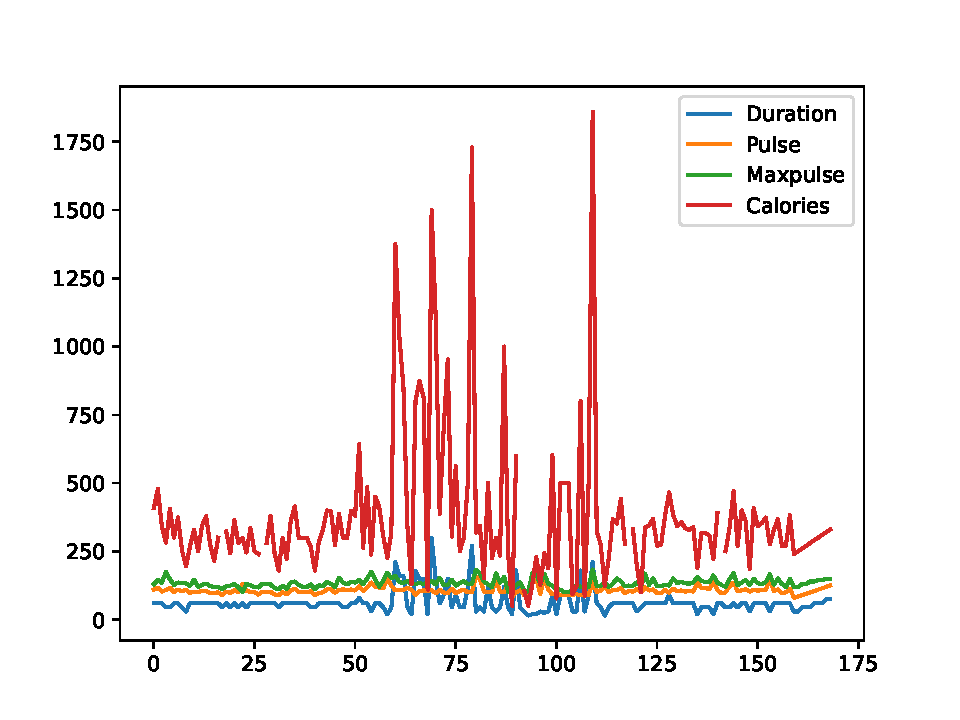
\includegraphics[scale=0.75]{img/grafica901.pdf}
  \caption{Visualización de un DataFrame}  
\end{figure}
\end{code}

\subsection{Diagrama de dispersión}

Especifique que desea un gráfico de dispersión con el argumento \texttt{kind}.
 
\begin{Shaded}
\begin{Highlighting}[]
\NormalTok{kind }\OperatorTok{=} \StringTok{\textquotesingle{}scatter\textquotesingle{}}
\end{Highlighting}
\end{Shaded}

Un diagrama de dispersión necesita un eje x y un eje y.

En el código \ref{code:dispersion}, utilizaremos ``Duración'' para el eje x y ``Calorías'' para el eje y.

Incluya los argumentos x e y de la siguiente manera:

\begin{Shaded}
  \begin{Highlighting}[]
    \NormalTok{x }\OperatorTok{=} \StringTok{\textquotesingle{}Duration\textquotesingle{}}\NormalTok{, y }\OperatorTok{=} \StringTok{\textquotesingle{}Calories\textquotesingle{}}

  \end{Highlighting}
\end{Shaded}


\begin{code} Diagrama de dispersión.

\begin{Shaded}
\begin{Highlighting}[]
\ImportTok{import}\NormalTok{ pandas }\ImportTok{as}\NormalTok{ pd}
\ImportTok{import}\NormalTok{ matplotlib.pyplot }\ImportTok{as}\NormalTok{ plt}

\NormalTok{df }\OperatorTok{=}\NormalTok{ pd.read\_csv(}\StringTok{\textquotesingle{}data/data.csv\textquotesingle{}}\NormalTok{)}

\NormalTok{df.plot(kind }\OperatorTok{=} \StringTok{\textquotesingle{}scatter\textquotesingle{}}\NormalTok{, x }\OperatorTok{=} \StringTok{\textquotesingle{}Duration\textquotesingle{}}\NormalTok{, y }\OperatorTok{=} \StringTok{\textquotesingle{}Calories\textquotesingle{}}\NormalTok{)}

\NormalTok{plt.show()}
\end{Highlighting}
\end{Shaded}

\begin{figure}[H]
  \centering
  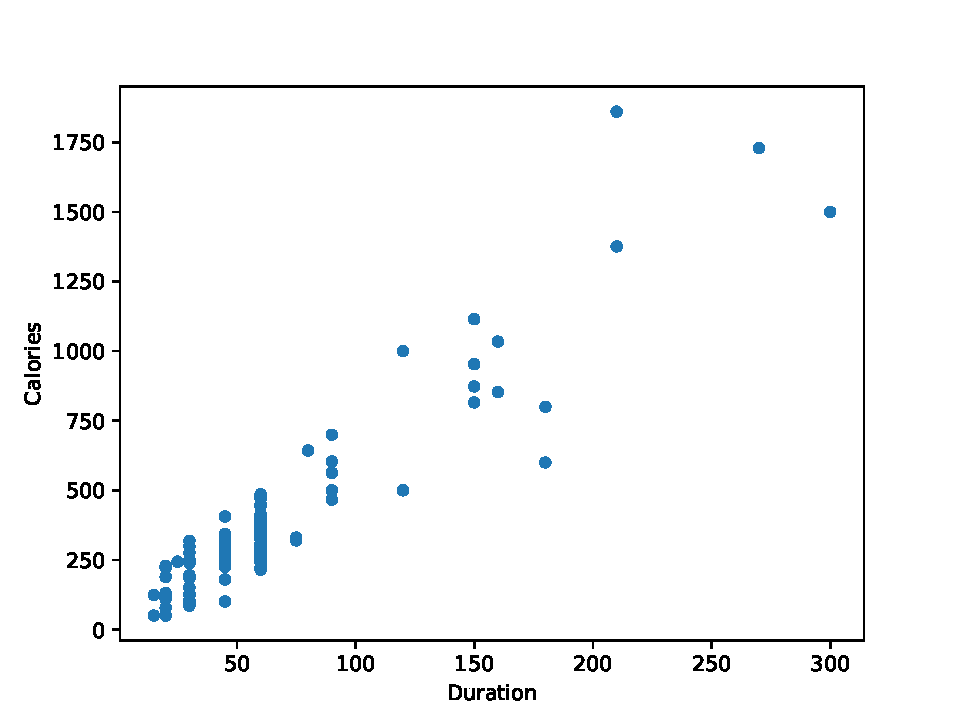
\includegraphics[scale=0.75]{img/grafica902.pdf}
  \caption{Diagrama de dispersión}
\end{figure}
\label{code:dispersion}
\end{code}
En la sección anterior, aprendimos que la correlación entre ``Duración'' y
``Calorías'' era 0.922721, y concluimos con el hecho de que una mayor
duración significa más calorías quemadas.

Al observar el diagrama de dispersión, podemos observar esa relación.

Creemos otro diagrama de dispersión, donde hay una mala relación entre
las columnas, como ``Duración'' y ``Pulso máximo'', con la correlación
0.009403.\\

\begin{code} Un diagrama de dispersión donde no hay relación entre las columnas.

\begin{Shaded}
\begin{Highlighting}[]
\ImportTok{import}\NormalTok{ pandas }\ImportTok{as}\NormalTok{ pd}
\ImportTok{import}\NormalTok{ matplotlib.pyplot }\ImportTok{as}\NormalTok{ plt}

\NormalTok{df }\OperatorTok{=}\NormalTok{ pd.read\_csv(}\StringTok{\textquotesingle{}data/data.csv\textquotesingle{}}\NormalTok{)}

\NormalTok{df.plot(kind }\OperatorTok{=} \StringTok{\textquotesingle{}scatter\textquotesingle{}}\NormalTok{, x }\OperatorTok{=} \StringTok{\textquotesingle{}Duration\textquotesingle{}}\NormalTok{, y }\OperatorTok{=} \StringTok{\textquotesingle{}Maxpulse\textquotesingle{}}\NormalTok{)}

\NormalTok{plt.show()}
\end{Highlighting}
\end{Shaded}

\begin{figure}
  \centering
  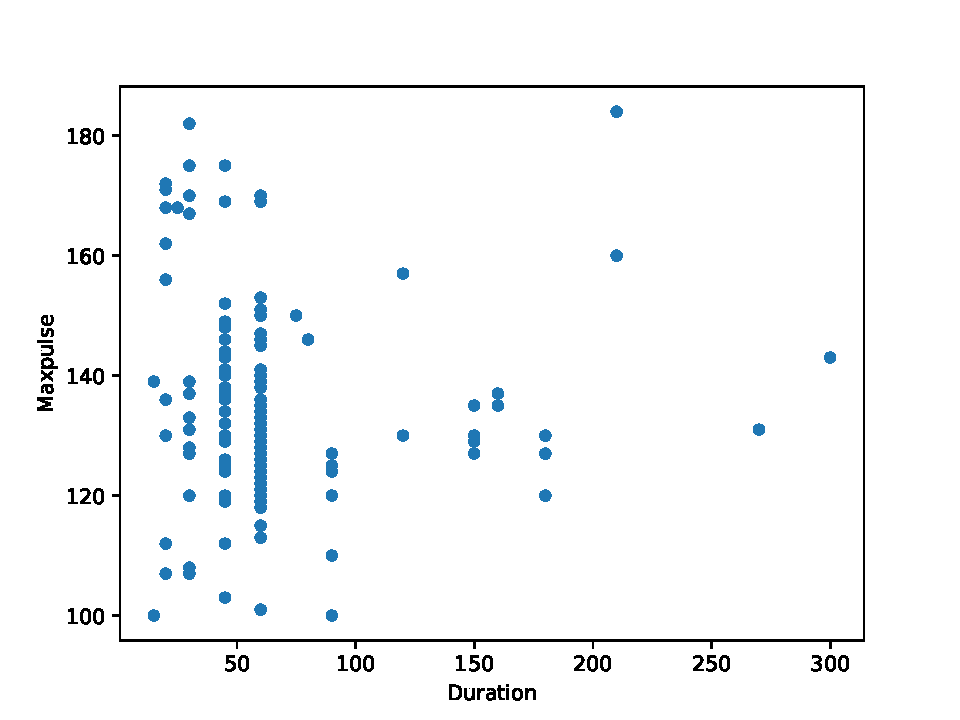
\includegraphics[scale=0.75]{img/grafica903.pdf}
  \caption{Diagrama de dispersión sin relación entre columnas}
\end{figure}
\end{code}

\subsection{Histograma}

Utilice el kindargumento para especificar que desea un histograma:
\begin{Shaded}
\begin{Highlighting}[]
\NormalTok{kind }\OperatorTok{=} \StringTok{\textquotesingle{}hist\textquotesingle{}}
\end{Highlighting}
\end{Shaded}

Un histograma solo necesita una columna. Un histograma nos muestra la
frecuencia de cada intervalo, por ejemplo ¿cuántos entrenamientos
duraron entre 50 y 60 minutos?

En el siguiente ejemplo, utilizaremos la columna "Duración" para crear
el histograma.\\

\begin{code} Histograma de un DataFrame.

\begin{Shaded}
\begin{Highlighting}[]
\NormalTok{df[}\StringTok{"Duration"}\NormalTok{].plot(kind }\OperatorTok{=} \StringTok{\textquotesingle{}hist\textquotesingle{}}\NormalTok{)}
\end{Highlighting}
\end{Shaded}

\begin{verbatim}
<Axes: ylabel='Frequency'>
\end{verbatim}

\begin{figure}
  \centering
  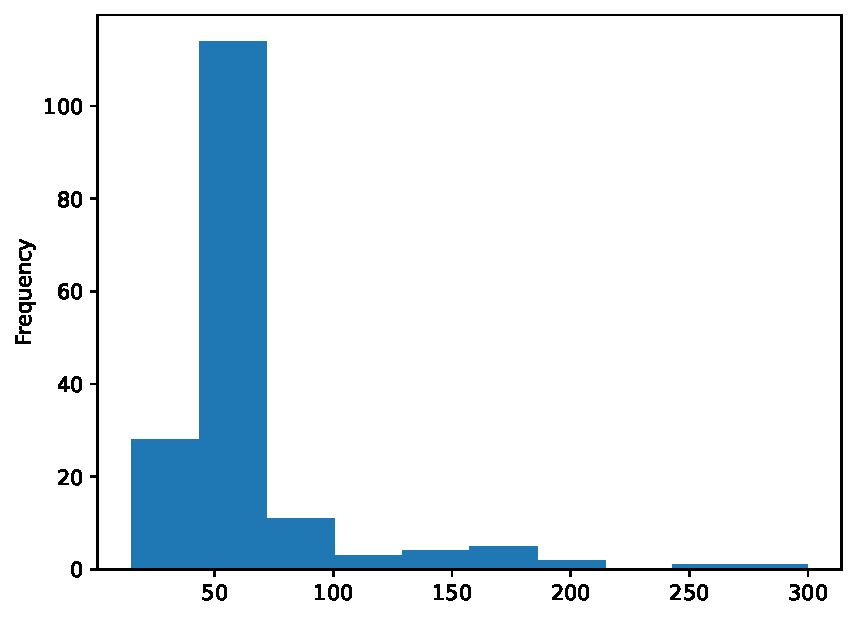
\includegraphics[scale=0.75]{img/grafica904.pdf}  
  \caption{Histograma de un DataFrame}
\end{figure}

\end{code}

El histograma nos dice que hay más de 100 ejercicios que duraron entre
50 y 60 minutos. \\

\begin{code} Ahora un histograma para las calorías.

\begin{Shaded}
\begin{Highlighting}[]
\NormalTok{df[}\StringTok{"Calories"}\NormalTok{].plot(kind }\OperatorTok{=} \StringTok{\textquotesingle{}hist\textquotesingle{}}\NormalTok{)}
\end{Highlighting}
\end{Shaded}

\begin{verbatim}
<Axes: ylabel='Frequency'>
\end{verbatim}

\begin{figure}
  \centering
  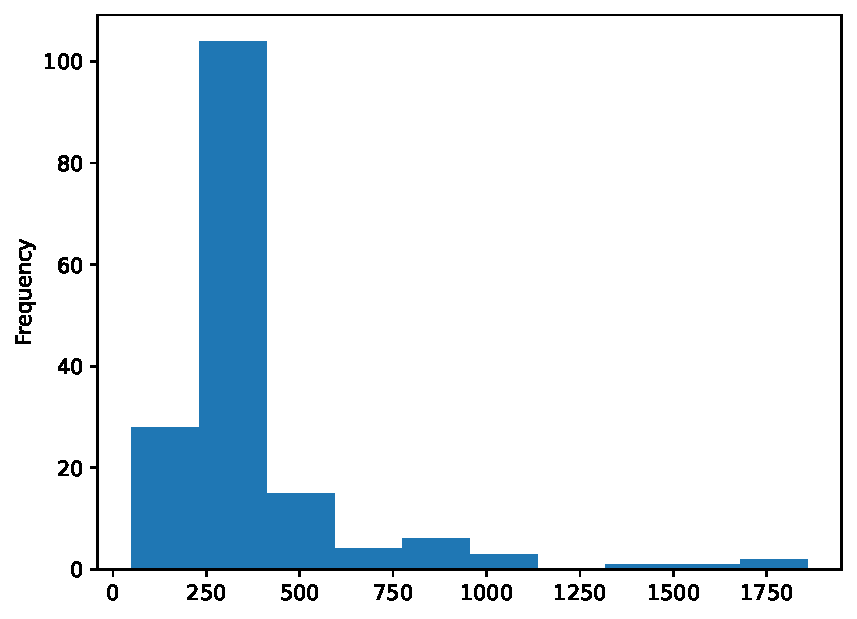
\includegraphics[scale=0.75]{img/grafica905.pdf}
  \caption{Histograma para las calorías}
\end{figure}
% \includegraphics{2c08fca6a1fb44b852da8706875c324b9e66d13e.png}
\end{code}

Este histograma nos dice que hubo poco más de 100 casos donde las
calorías quemadas fueron entre 250 y 300.

Dado que el método \texttt{plot} de Pandas utiliza \texttt{matplotlib}
como backend, si se desea modificar aspectos finos de la gráfica se debe
hacer configurando el gráfico a través de \texttt{matplotlib}
directamente.

\section{Referencias}

\begin{itemize}
  \item \href{https://www.w3schools.com/python/python_file_handling.asp}{Manejo de archivos en Python.}
  \item Lutz M., Learning Python, O\textquotesingle Reilly. 2009 
  \item \href{https://pandas.pydata.org/}{Pandas, sitio oficial.}
  \item \href{https://www.w3schools.com/python/pandas/default.asp}{Pandas en la W3Schools.}
  \item \href{https://pandas.pydata.org/docs/reference/api/pandas.DataFrame.plot.html}{Pandas Plot}
\end{itemize}


    % Chapter 10
    \chapter{Matplotlib}

Matplotlib es una biblioteca de trazado de gráficos de bajo nivel en
Python que sirve como una utilidad de visualización.

Matplotlib es de código abierto y fue creado por John D. Hunter.

Está escrito principalmente en Python, algunos segmentos están escritos
en C, Objective-C y Javascript.

\section{Comprobar versión de matplotlib}

Una vez que \texttt{matplotlib} esté instalado es necesario importarlo.
Se puede verificar la versión del paquete con el comando.

\begin{Shaded}
\begin{Highlighting}[]
\ImportTok{import}\NormalTok{ matplotlib}
\BuiltInTok{print}\NormalTok{(matplotlib.\_\_version\_\_)}
\end{Highlighting}
\end{Shaded}

\begin{verbatim}
3.8.3
\end{verbatim}

\section{Pyplot}

La mayoría de las utilidades de \texttt{Matplotlib} se encuentran bajo
el submódulo \texttt{pyplot}, y generalmente se importan bajo el alias
\texttt{plt}:

\begin{Shaded}
\begin{Highlighting}[]
\ImportTok{import}\NormalTok{ matplotlib.pyplot }\ImportTok{as}\NormalTok{ plt}
\end{Highlighting}
\end{Shaded}

Ahora el paquete \texttt{Pyplot} se puede denominar \texttt{plt}.\\

\begin{code} Dibuja una línea en un diagrama desde la posición \((0,0)\) hasta la posición \((6,250)\).

\begin{Shaded}
\begin{Highlighting}[]
\ImportTok{import}\NormalTok{ matplotlib.pyplot }\ImportTok{as}\NormalTok{ plt}
\ImportTok{import}\NormalTok{ numpy }\ImportTok{as}\NormalTok{ np}

\NormalTok{xpoints }\OperatorTok{=}\NormalTok{ np.array([}\DecValTok{0}\NormalTok{, }\DecValTok{6}\NormalTok{])}
\NormalTok{ypoints }\OperatorTok{=}\NormalTok{ np.array([}\DecValTok{0}\NormalTok{, }\DecValTok{250}\NormalTok{])}

\NormalTok{plt.plot(xpoints, ypoints)}
\NormalTok{plt.show()}
\end{Highlighting}
\end{Shaded}
\begin{figure}
  \centering
  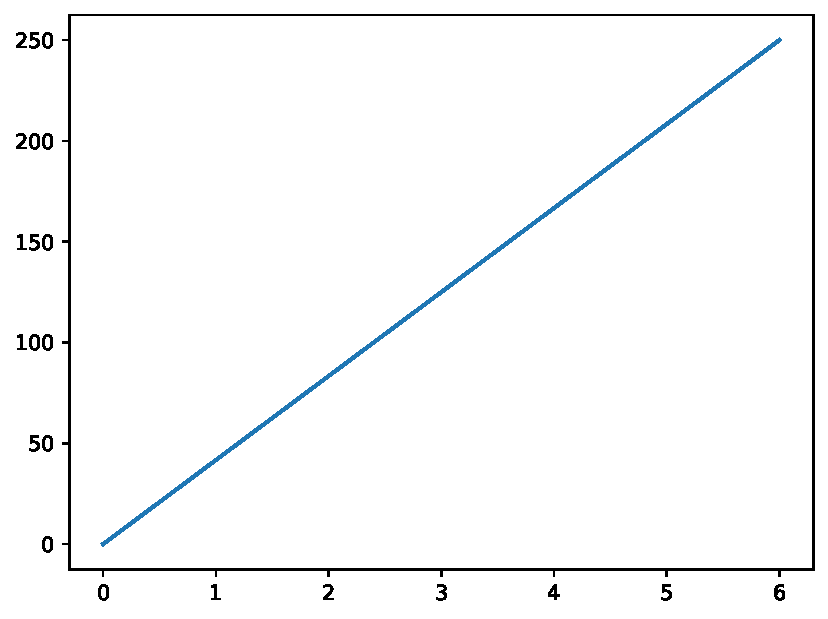
\includegraphics[scale=0.6]{img/grafica1001.pdf}
\end{figure}

\end{code}

\section{Graficas con matplotlib}

\subsection{\texorpdfstring{Gráfica puntos \((x, y)\)}{Gráfica puntos (x, y)}}

La función \texttt{plot()} se utiliza para dibujar puntos en un
diagrama. Por defecto, \texttt{plot()} dibuja una línea de punto a
punto.

La función toma parámetros para especificar puntos en el diagrama.

\begin{itemize}
  \item El parámetro 1 es una matriz que contiene los puntos en el eje X.
  \item El parámetro 2 es una matriz que contiene los puntos en el eje Y.
\end{itemize}

Si necesitamos trazar una línea de (1, 3) a (8, 10), tenemos que pasar
dos matrices {[}1, 8{]} y {[}3, 10{]} a la función de trazado.\\

\begin{code} Dibuje una línea en un diagrama desde la posición (1, 3) a la posición (8, 10)

\begin{Shaded}
\begin{Highlighting}[]
\ImportTok{import}\NormalTok{ matplotlib.pyplot }\ImportTok{as}\NormalTok{ plt}
\ImportTok{import}\NormalTok{ numpy }\ImportTok{as}\NormalTok{ np}

\NormalTok{xpoints }\OperatorTok{=}\NormalTok{ np.array([}\DecValTok{1}\NormalTok{, }\DecValTok{8}\NormalTok{])}
\NormalTok{ypoints }\OperatorTok{=}\NormalTok{ np.array([}\DecValTok{3}\NormalTok{, }\DecValTok{10}\NormalTok{])}

\NormalTok{plt.plot(xpoints, ypoints)}
\NormalTok{plt.show()}
\end{Highlighting}
\end{Shaded}

\begin{figure}
  \centering
  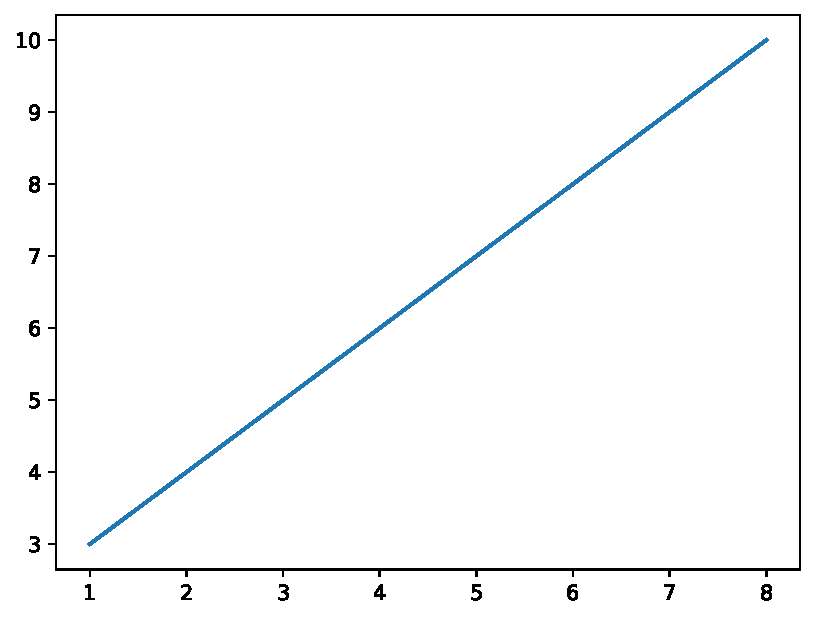
\includegraphics[scale=0.6]{img/grafica1002.pdf}
\end{figure}

\end{code}

\section{Gráfica Sin Línea}

Para trazar solo los marcadores, puede usar notación de cadena de acceso
directo parámetro \texttt{\textquotesingle{}o\textquotesingle{}}, que
significa \emph{\textquotesingle anillos\textquotesingle{}}.\\

\begin{code} Dibuja dos puntos en el diagrama, uno en posición (1, 3) y otro en posición (8, 10).

\begin{Shaded}
\begin{Highlighting}[]
\ImportTok{import}\NormalTok{ matplotlib.pyplot }\ImportTok{as}\NormalTok{ plt}
\ImportTok{import}\NormalTok{ numpy }\ImportTok{as}\NormalTok{ np}

\NormalTok{xpoints }\OperatorTok{=}\NormalTok{ np.array([}\DecValTok{1}\NormalTok{, }\DecValTok{8}\NormalTok{])}
\NormalTok{ypoints }\OperatorTok{=}\NormalTok{ np.array([}\DecValTok{3}\NormalTok{, }\DecValTok{10}\NormalTok{])}

\NormalTok{plt.plot(xpoints, ypoints, }\StringTok{\textquotesingle{}o\textquotesingle{}}\NormalTok{)}
\NormalTok{plt.show()}
\end{Highlighting}
\end{Shaded}

\begin{figure}
  \centering
  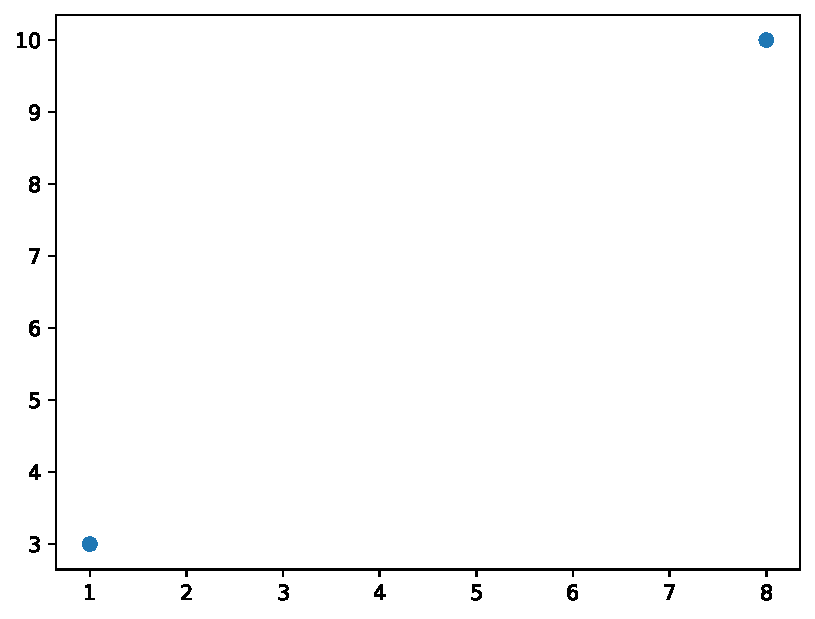
\includegraphics[scale=0.6]{img/grafica1003.pdf}
\end{figure}
\end{code}


\section{Múltiples Puntos}

Puede trazar tantos puntos como desee, solo asegúrese de tener el mismo
número de puntos en ambos ejes. \\

\begin{code} Dibuja una línea en un diagrama desde la posición
\((1, 3)\) a \((2, 8)\) luego a \((6, 1)\) y finalmente a la posición
\((8, 10)\)

\begin{Shaded}
\begin{Highlighting}[]
\ImportTok{import}\NormalTok{ matplotlib.pyplot }\ImportTok{as}\NormalTok{ plt}
\ImportTok{import}\NormalTok{ numpy }\ImportTok{as}\NormalTok{ np}

\NormalTok{xpoints }\OperatorTok{=}\NormalTok{ np.array([}\DecValTok{1}\NormalTok{, }\DecValTok{2}\NormalTok{, }\DecValTok{6}\NormalTok{, }\DecValTok{8}\NormalTok{])}
\NormalTok{ypoints }\OperatorTok{=}\NormalTok{ np.array([}\DecValTok{3}\NormalTok{, }\DecValTok{8}\NormalTok{, }\DecValTok{1}\NormalTok{, }\DecValTok{10}\NormalTok{])}

\NormalTok{plt.plot(xpoints, ypoints)}
\NormalTok{plt.show()}
\end{Highlighting}
\end{Shaded}

\begin{figure}
  \centering
  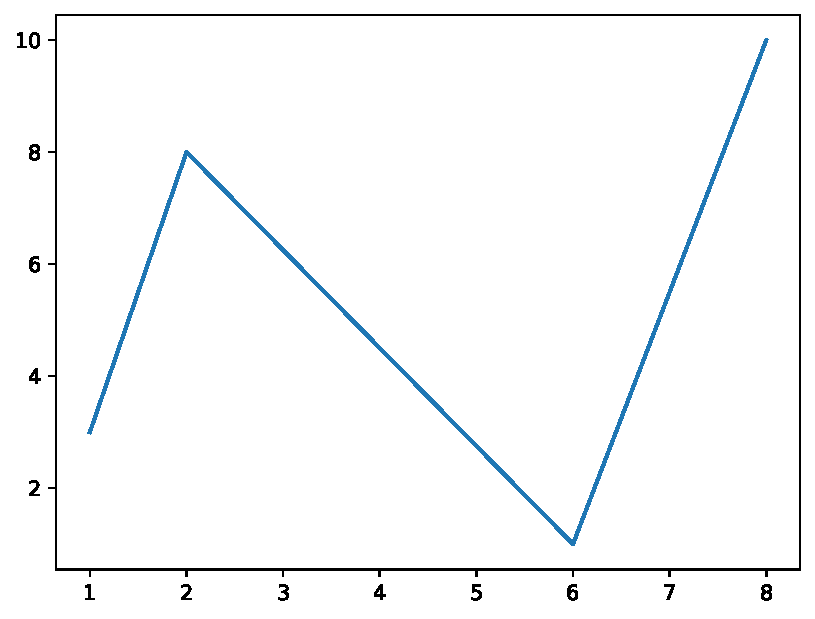
\includegraphics[scale=0.6]{img/grafica1004.pdf}
\end{figure}
\end{code}

\section{\texorpdfstring{Valores \(x\) predeterminados}{Valores x predeterminados}}

Si no especificamos los puntos en el eje \(x\), obtendrán los valores
predeterminados \(0, 1, 2, 3, \dots\), dependiendo de la longitud de los
puntos \(y\).

Entonces, si tomamos el mismo ejemplo que el anterior y dejamos de lado
los puntos \(x\), el diagrama se verá así:\\

\begin{code} Gráfica sin valores \(x\).

\begin{Shaded}
\begin{Highlighting}[]
\ImportTok{import}\NormalTok{ matplotlib.pyplot }\ImportTok{as}\NormalTok{ plt}
\ImportTok{import}\NormalTok{ numpy }\ImportTok{as}\NormalTok{ np}

\NormalTok{ypoints }\OperatorTok{=}\NormalTok{ np.array([}\DecValTok{3}\NormalTok{, }\DecValTok{8}\NormalTok{, }\DecValTok{1}\NormalTok{, }\DecValTok{10}\NormalTok{, }\DecValTok{5}\NormalTok{, }\DecValTok{7}\NormalTok{])}

\NormalTok{plt.plot(ypoints)}
\NormalTok{plt.show()}
\end{Highlighting}
\end{Shaded}

\begin{figure}
  \centering
  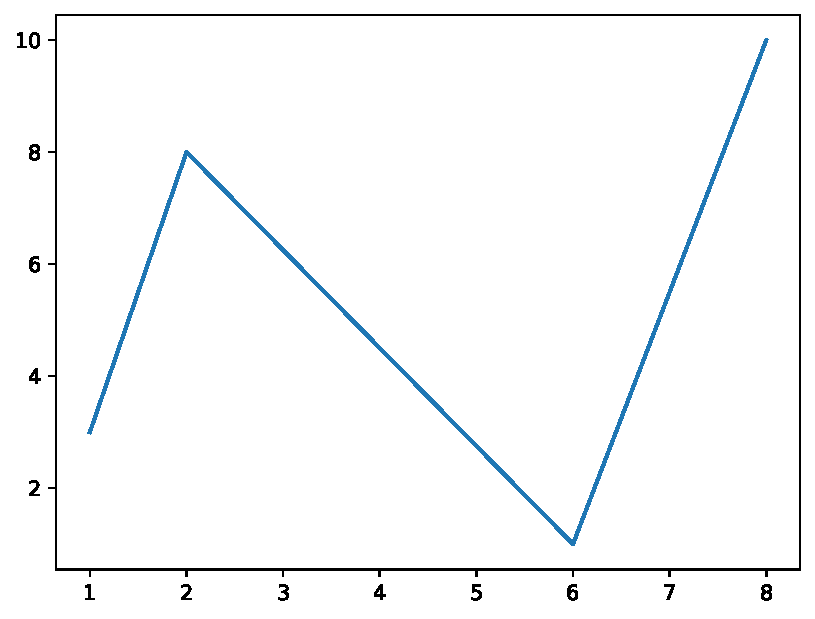
\includegraphics[scale=0.6]{img/grafica1004.pdf}
\end{figure}
\end{code}

\section{Marcadores}

Puede usar el argumento \texttt{marker} para enfatizar cada punto con un
marcador especifico.\\

\begin{code} Marcar cada punto con un círculo.

\begin{Shaded}
\begin{Highlighting}[]
\ImportTok{import}\NormalTok{ matplotlib.pyplot }\ImportTok{as}\NormalTok{ plt}
\ImportTok{import}\NormalTok{ numpy }\ImportTok{as}\NormalTok{ np}

\NormalTok{ypoints }\OperatorTok{=}\NormalTok{ np.array([}\DecValTok{3}\NormalTok{, }\DecValTok{8}\NormalTok{, }\DecValTok{1}\NormalTok{, }\DecValTok{10}\NormalTok{])}

\NormalTok{plt.plot(ypoints, marker }\OperatorTok{=} \StringTok{\textquotesingle{}o\textquotesingle{}}\NormalTok{)}
\NormalTok{plt.show()}
\end{Highlighting}
\end{Shaded}

\begin{figure}
  \centering
  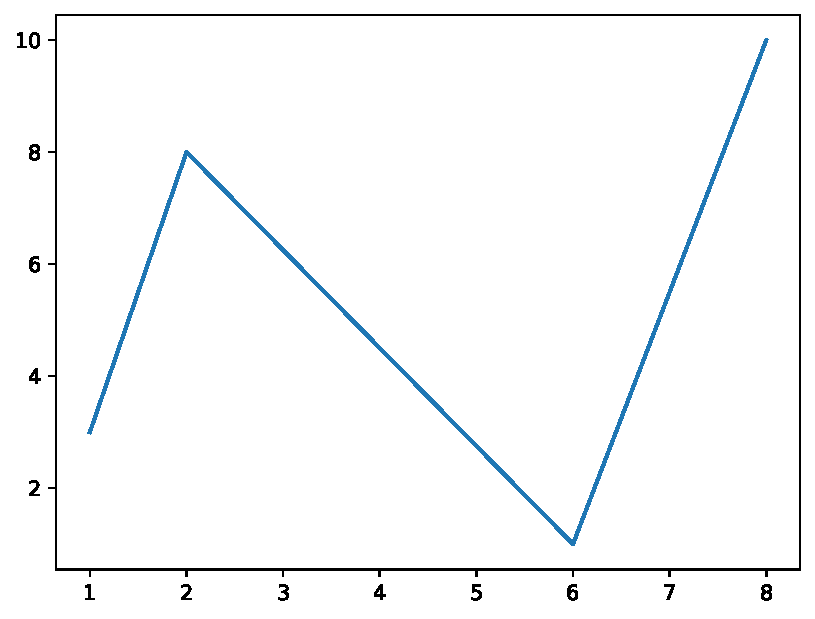
\includegraphics[scale=0.6]{img/grafica1004.pdf}
\end{figure}
\end{code}


\begin{code} Marca cada punto con una estrella.

\begin{Shaded}
\begin{Highlighting}[]
\ImportTok{import}\NormalTok{ matplotlib.pyplot }\ImportTok{as}\NormalTok{ plt}
\ImportTok{import}\NormalTok{ numpy }\ImportTok{as}\NormalTok{ np}

\NormalTok{ypoints }\OperatorTok{=}\NormalTok{ np.array([}\DecValTok{3}\NormalTok{, }\DecValTok{8}\NormalTok{, }\DecValTok{1}\NormalTok{, }\DecValTok{10}\NormalTok{])}

\NormalTok{plt.plot(ypoints, marker }\OperatorTok{=} \StringTok{\textquotesingle{}*\textquotesingle{}}\NormalTok{)}
\NormalTok{plt.show()}
\end{Highlighting}
\end{Shaded}

\begin{figure}
  \centering
  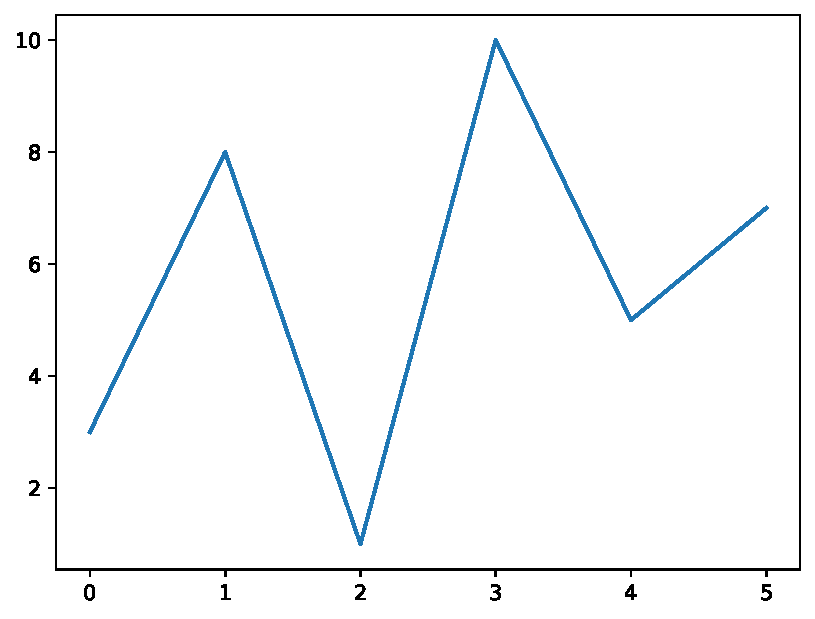
\includegraphics[scale=0.6]{img/grafica1005.pdf}
\end{figure}
\end{code}

\subsection{Referencia de los marcadores}

Puede elegir cualquiera de estos marcadores:

\begin{longtable}[]{@{}cc@{}}
\toprule\noalign{}
Marker & Description \\
\midrule\noalign{}
\endhead
\bottomrule\noalign{}
\endlastfoot
\textquotesingle o\textquotesingle{} & Circle \\
\textquotesingle*\textquotesingle{} & Star \\
\textquotesingle.\textquotesingle{} & Point \\
\textquotesingle,\textquotesingle{} & Pixel \\
\textquotesingle x\textquotesingle{} & X \\
\textquotesingle X\textquotesingle{} & X (filled) \\
\textquotesingle+\textquotesingle{} & Plus \\
\textquotesingle P\textquotesingle{} & Plus (filled) \\
\textquotesingle s\textquotesingle{} & Square \\
\textquotesingle D\textquotesingle{} & Diamond \\
\textquotesingle d\textquotesingle{} & Diamond (thin) \\
\textquotesingle p\textquotesingle{} & Pentagon \\
\textquotesingle H\textquotesingle{} & Hexagon \\
\textquotesingle h\textquotesingle{} & Hexagon \\
\textquotesingle v\textquotesingle{} & Triangle Down \\
\textquotesingle\^{}\textquotesingle{} & Triangle Up \\
\textquotesingle\textless\textquotesingle{} & Triangle Left \\
\textquotesingle\textgreater\textquotesingle{} & Triangle Right \\
\textquotesingle1\textquotesingle{} & Tri Down \\
\textquotesingle2\textquotesingle{} & Tri Up \\
\textquotesingle3\textquotesingle{} & Tri Left \\
\textquotesingle4\textquotesingle{} & Tri Right \\
\textquotesingle{} & \textquotesingle{} \\
\textquotesingle\_\textquotesingle{} & Hline \\
\end{longtable}

\begin{code} Marcador cuadrado.
\begin{Shaded}
\begin{Highlighting}[]
\NormalTok{plt.plot(ypoints, marker }\OperatorTok{=} \StringTok{\textquotesingle{}s\textquotesingle{}}\NormalTok{)}
\NormalTok{plt.show()}
\end{Highlighting}
\end{Shaded}

\begin{figure}
  \centering
  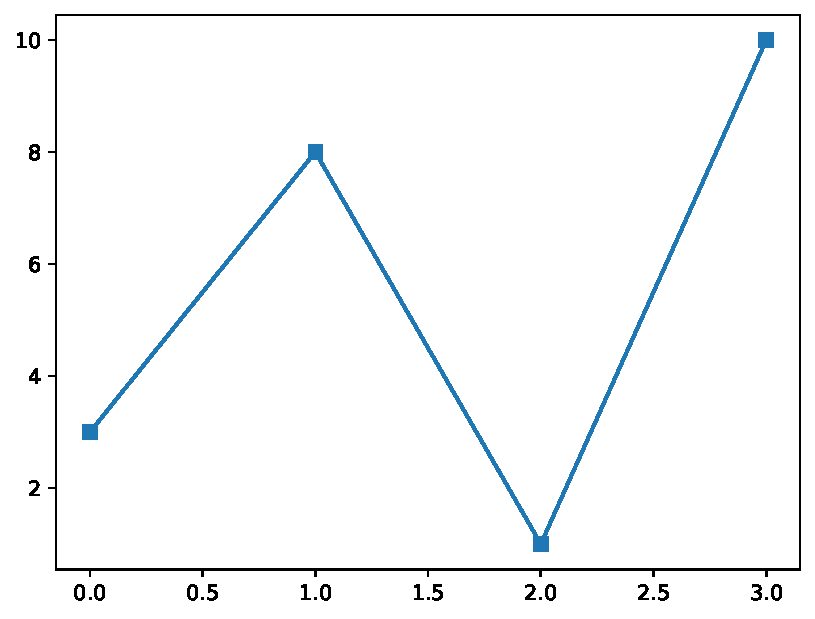
\includegraphics[scale=0.6]{img/grafica1008.pdf}
\end{figure}
\end{code}

\section{\texorpdfstring{Formato cadena \texttt{fmt}}{Formato cadena fmt}}

También puedes usar el notación de cadena de acceso directo parámetro
para especificar el marcador.

Este parámetro también se llama \texttt{fmt} y está escrito con esta
sintaxis:

\begin{Shaded}
\begin{Highlighting}[]
\NormalTok{marker}\OperatorTok{|}\NormalTok{line}\OperatorTok{|}\NormalTok{color}

\end{Highlighting}
\end{Shaded}

\begin{code} Marque cada punto con un círculo.

\begin{Shaded}
\begin{Highlighting}[]
\ImportTok{import}\NormalTok{ matplotlib.pyplot }\ImportTok{as}\NormalTok{ plt}
\ImportTok{import}\NormalTok{ numpy }\ImportTok{as}\NormalTok{ np}

\NormalTok{ypoints }\OperatorTok{=}\NormalTok{ np.array([}\DecValTok{3}\NormalTok{, }\DecValTok{8}\NormalTok{, }\DecValTok{1}\NormalTok{, }\DecValTok{10}\NormalTok{])}

\NormalTok{plt.plot(ypoints, }\StringTok{\textquotesingle{}o:g\textquotesingle{}}\NormalTok{)}
\NormalTok{plt.show()}
\end{Highlighting}
\end{Shaded}

\begin{figure}
  \centering
  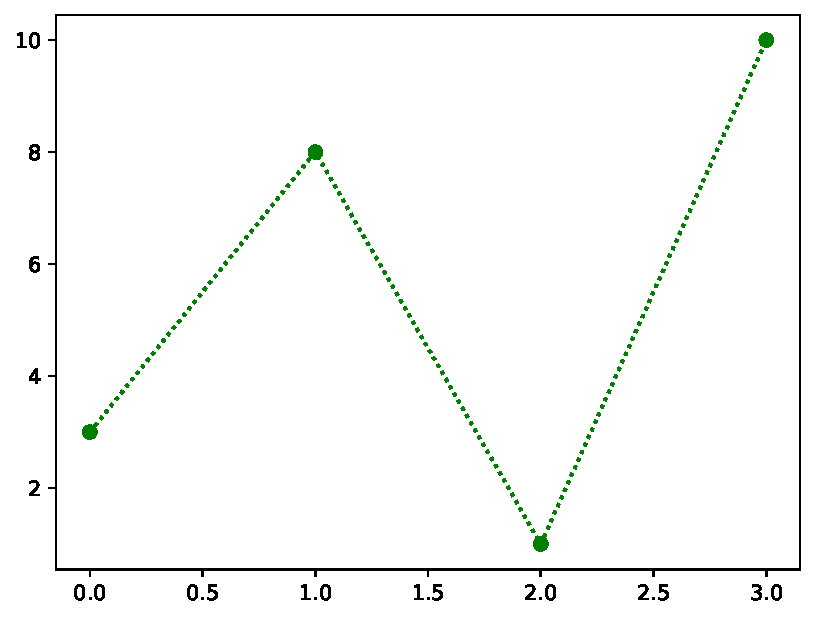
\includegraphics[scale=0.6]{img/grafica1009.pdf}
\end{figure}

\end{code}

El valor del marcador puede ser cualquier cosa de la Referencia del
Marcador anterior.

El valor de la línea puede ser uno de los siguientes:

\subsection{Referencia de Línea}

\begin{longtable}[]{@{}cc@{}}
\toprule\noalign{}
Sintaxis línea & Descripción \\
\midrule\noalign{}
\endhead
\bottomrule\noalign{}
\endlastfoot
\textquotesingle-\textquotesingle{} & Solid line \\
\textquotesingle:\textquotesingle{} & Dotted line 1 \\
\end{longtable}

\textquotesingle-\/-\textquotesingle{} Dashed line
\textquotesingle-.\textquotesingle{} Dashed/dotted line

\begin{Shaded}
\begin{Highlighting}[]
\NormalTok{plt.plot(ypoints, }\StringTok{\textquotesingle{}o{-}.g\textquotesingle{}}\NormalTok{)}
\NormalTok{plt.show()}
\end{Highlighting}
\end{Shaded}

\begin{figure}
  \centering
  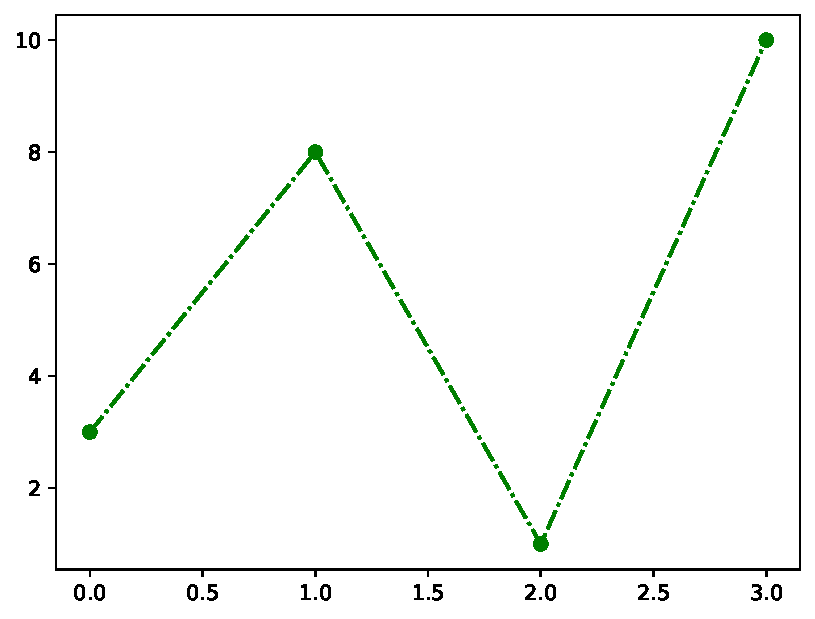
\includegraphics[scale=0.6]{img/grafica1010.pdf}
\end{figure}


\subsection{Referencia de Color}

\begin{longtable}[]{@{}cc@{}}
\toprule\noalign{}
Sintaxis & Descripción \\
\midrule\noalign{}
\endhead
\bottomrule\noalign{}
\endlastfoot
\textquotesingle r\textquotesingle{} & Red \\
\textquotesingle g\textquotesingle{} & Green \\
\textquotesingle b\textquotesingle{} & Blue \\
\textquotesingle c\textquotesingle{} & Cyan \\
\textquotesingle m\textquotesingle{} & Magenta \\
\textquotesingle y\textquotesingle{} & Yellow \\
\textquotesingle k\textquotesingle{} & Black \\
\textquotesingle w\textquotesingle{} & White \\
\end{longtable}

\subsection{Tamaño del Marcador}

Puede usar el argumento de palabra clave \texttt{markersize} o la
versión más corta, \texttt{ms} para establecer el tamaño de los
marcadores.\\

\begin{code} Establezca el tamaño de los marcadores en 20.

\begin{Shaded}
\begin{Highlighting}[]
\ImportTok{import}\NormalTok{ matplotlib.pyplot }\ImportTok{as}\NormalTok{ plt}
\ImportTok{import}\NormalTok{ numpy }\ImportTok{as}\NormalTok{ np}

\NormalTok{ypoints }\OperatorTok{=}\NormalTok{ np.array([}\DecValTok{3}\NormalTok{, }\DecValTok{8}\NormalTok{, }\DecValTok{1}\NormalTok{, }\DecValTok{10}\NormalTok{])}

\NormalTok{plt.plot(ypoints, marker }\OperatorTok{=} \StringTok{\textquotesingle{}o\textquotesingle{}}\NormalTok{, ms }\OperatorTok{=} \DecValTok{20}\NormalTok{)}
\NormalTok{plt.show()}
\end{Highlighting}
\end{Shaded}

\begin{figure}
  \centering
  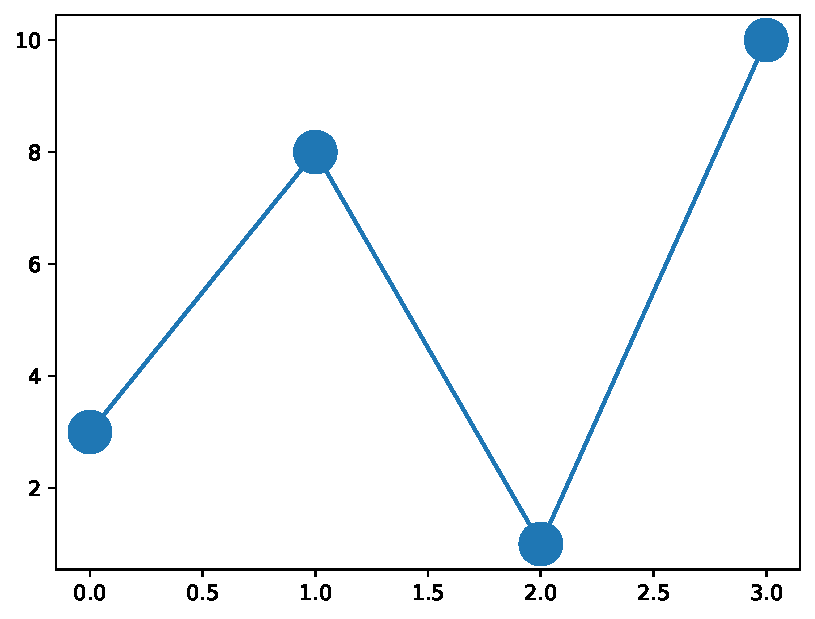
\includegraphics[scale=0.6]{img/grafica1011.pdf}
\end{figure}

\end{code}

\subsection{Color del Marcador}

Puede usar el argumento de palabra clave \texttt{markeredgecolor} o el
más corto \texttt{mec} para establecer el color de la borde de los
marcadores.\\

\begin{code} Establezca el color EDGE en rojo.

\begin{Shaded}
\begin{Highlighting}[]
\ImportTok{import}\NormalTok{ matplotlib.pyplot }\ImportTok{as}\NormalTok{ plt}
\ImportTok{import}\NormalTok{ numpy }\ImportTok{as}\NormalTok{ np}

\NormalTok{ypoints }\OperatorTok{=}\NormalTok{ np.array([}\DecValTok{3}\NormalTok{, }\DecValTok{8}\NormalTok{, }\DecValTok{1}\NormalTok{, }\DecValTok{10}\NormalTok{])}

\NormalTok{plt.plot(ypoints, marker }\OperatorTok{=} \StringTok{\textquotesingle{}o\textquotesingle{}}\NormalTok{, ms }\OperatorTok{=} \DecValTok{20}\NormalTok{, mec }\OperatorTok{=} \StringTok{\textquotesingle{}r\textquotesingle{}}\NormalTok{)}
\NormalTok{plt.show()}
\end{Highlighting}
\end{Shaded}

\begin{figure}
  \centering
  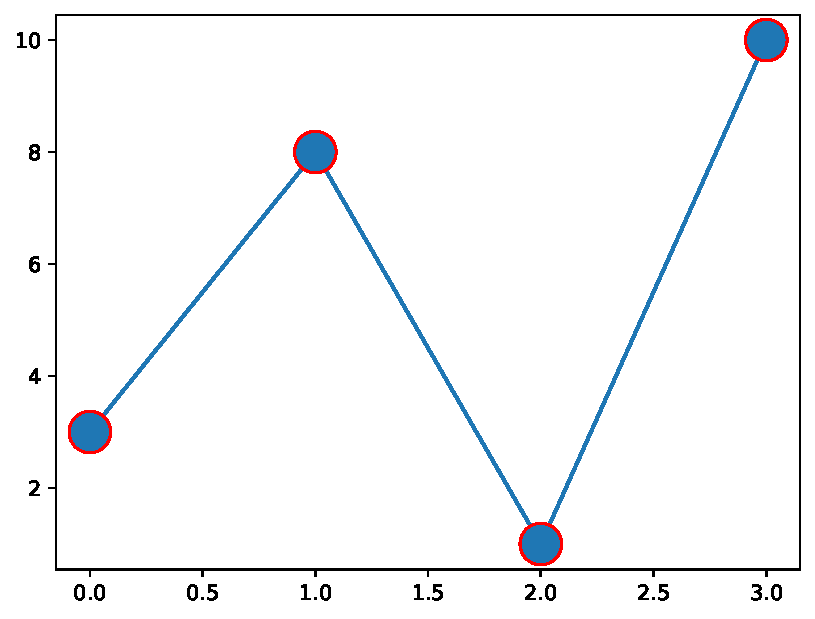
\includegraphics[scale=0.6]{img/grafica1012.pdf}
\end{figure}

\end{code}

Puede usar el argumento de palabra clave \texttt{markerfacecolor} o el
más corto \texttt{mfc} para establecer el color dentro del borde de los
marcadores:\\

\begin{code} Coloque el color FACE en rojo.

\begin{Shaded}
\begin{Highlighting}[]
\ImportTok{import}\NormalTok{ matplotlib.pyplot }\ImportTok{as}\NormalTok{ plt}
\ImportTok{import}\NormalTok{ numpy }\ImportTok{as}\NormalTok{ np}

\NormalTok{ypoints }\OperatorTok{=}\NormalTok{ np.array([}\DecValTok{3}\NormalTok{, }\DecValTok{8}\NormalTok{, }\DecValTok{1}\NormalTok{, }\DecValTok{10}\NormalTok{])}

\NormalTok{plt.plot(ypoints, marker }\OperatorTok{=} \StringTok{\textquotesingle{}o\textquotesingle{}}\NormalTok{, ms }\OperatorTok{=} \DecValTok{20}\NormalTok{, mfc }\OperatorTok{=} \StringTok{\textquotesingle{}r\textquotesingle{}}\NormalTok{)}
\NormalTok{plt.show()}
\end{Highlighting}
\end{Shaded}

\begin{figure}
  \centering
  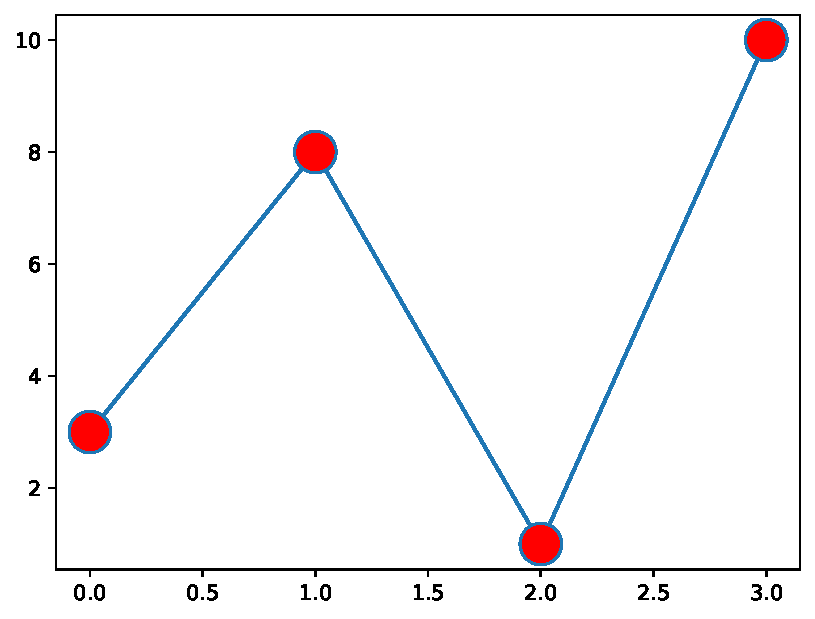
\includegraphics[scale=0.6]{img/grafica1013.pdf}
\end{figure}
\end{code}

Usar ambos el \texttt{mec} y \texttt{mfc} argumentos para colorear todo
el marcador:\\

\begin{code} Establezca el color de ambos borde y el cara a rojo.

\begin{Shaded}
\begin{Highlighting}[]
\ImportTok{import}\NormalTok{ matplotlib.pyplot }\ImportTok{as}\NormalTok{ plt}
\ImportTok{import}\NormalTok{ numpy }\ImportTok{as}\NormalTok{ np}

\NormalTok{ypoints }\OperatorTok{=}\NormalTok{ np.array([}\DecValTok{3}\NormalTok{, }\DecValTok{8}\NormalTok{, }\DecValTok{1}\NormalTok{, }\DecValTok{10}\NormalTok{])}

\NormalTok{plt.plot(ypoints, marker }\OperatorTok{=} \StringTok{\textquotesingle{}o\textquotesingle{}}\NormalTok{, ms }\OperatorTok{=} \DecValTok{20}\NormalTok{, mec }\OperatorTok{=} \StringTok{\textquotesingle{}r\textquotesingle{}}\NormalTok{, mfc }\OperatorTok{=} \StringTok{\textquotesingle{}r\textquotesingle{}}\NormalTok{)}
\NormalTok{plt.show()}
\end{Highlighting}
\end{Shaded}

\begin{figure}
  \centering
  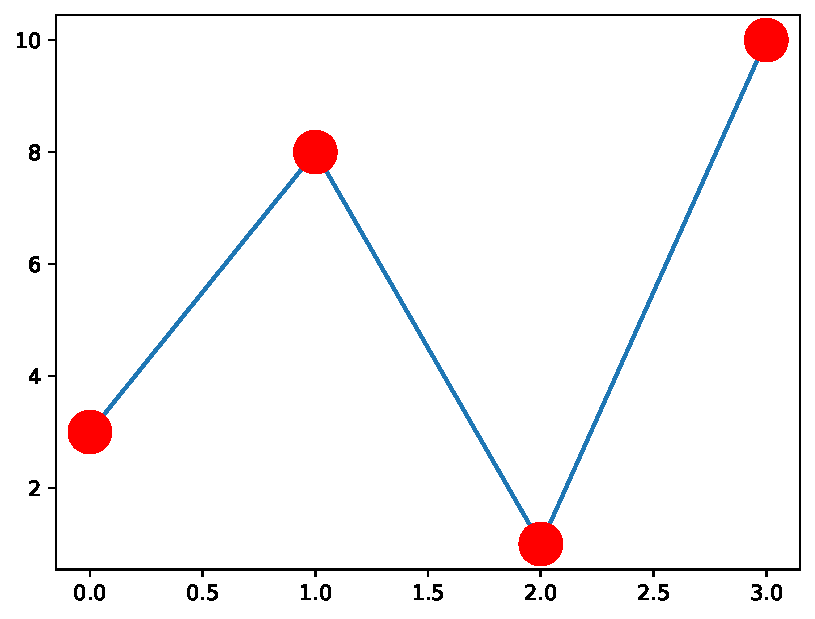
\includegraphics[scale=0.6]{img/grafica1014.pdf}
\end{figure}

\end{code}

También puedes usar valores de color hexadecimal, o cualquiera de los
140 \href{https://www.w3schools.com/colors/colors_names.asp}{nombres de
color} compatibles.

\begin{code} Marque cada punto con un hermoso color verde.

\begin{Shaded}
\begin{Highlighting}[]
\NormalTok{plt.plot(ypoints, marker }\OperatorTok{=} \StringTok{\textquotesingle{}o\textquotesingle{}}\NormalTok{, ms }\OperatorTok{=} \DecValTok{20}\NormalTok{, mec }\OperatorTok{=} \StringTok{\textquotesingle{}\#4CAF50\textquotesingle{}}\NormalTok{, mfc }\OperatorTok{=} \StringTok{\textquotesingle{}\#4CAF50\textquotesingle{}}\NormalTok{)}
\NormalTok{plt.show()}
\end{Highlighting}
\end{Shaded}

\begin{figure}
  \centering
  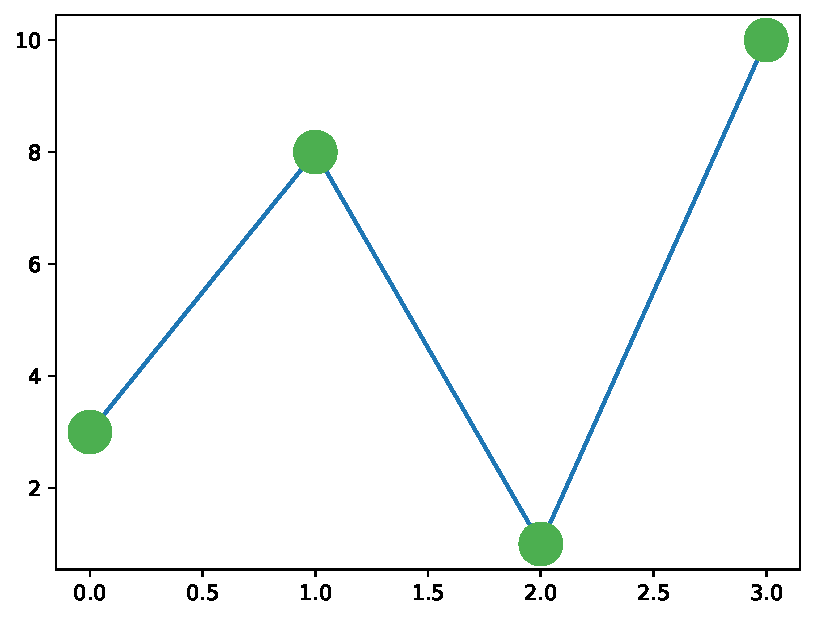
\includegraphics[scale=0.6]{img/grafica1015.pdf}
\end{figure}

\end{code}

\section{Estilo de línea}

Puede usar el argumento de palabra clave \texttt{linestyle}, o más corto
\texttt{ls}, a cambiar el estilo de la línea trazada.\\

\begin{code} Usa una línea punteada.

\begin{Shaded}
\begin{Highlighting}[]
\ImportTok{import}\NormalTok{ matplotlib.pyplot }\ImportTok{as}\NormalTok{ plt}
\ImportTok{import}\NormalTok{ numpy }\ImportTok{as}\NormalTok{ np}

\NormalTok{ypoints }\OperatorTok{=}\NormalTok{ np.array([}\DecValTok{3}\NormalTok{, }\DecValTok{8}\NormalTok{, }\DecValTok{1}\NormalTok{, }\DecValTok{10}\NormalTok{])}

\NormalTok{plt.plot(ypoints, linestyle }\OperatorTok{=} \StringTok{\textquotesingle{}dotted\textquotesingle{}}\NormalTok{)}
\NormalTok{plt.show()}
\end{Highlighting}
\end{Shaded}

\begin{figure}
  \centering
  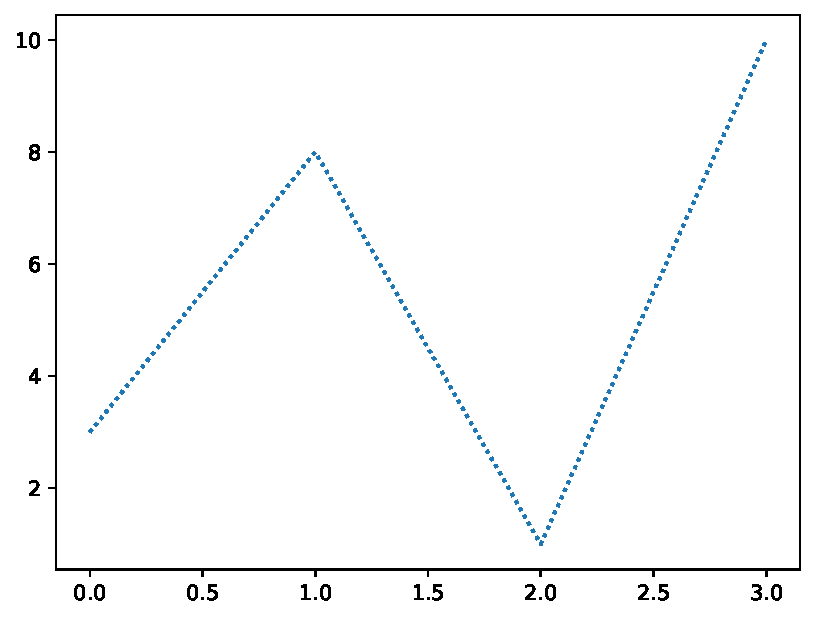
\includegraphics[scale=0.6]{img/grafica1016.pdf}
\end{figure}

\end{code}

\begin{code} Usa una línea discontinua.

\begin{Shaded}
\begin{Highlighting}[]
\NormalTok{plt.plot(ypoints, linestyle }\OperatorTok{=} \StringTok{\textquotesingle{}dashed\textquotesingle{}}\NormalTok{)}
\NormalTok{plt.show()}
\end{Highlighting}
\end{Shaded}

\begin{figure}
  \centering
  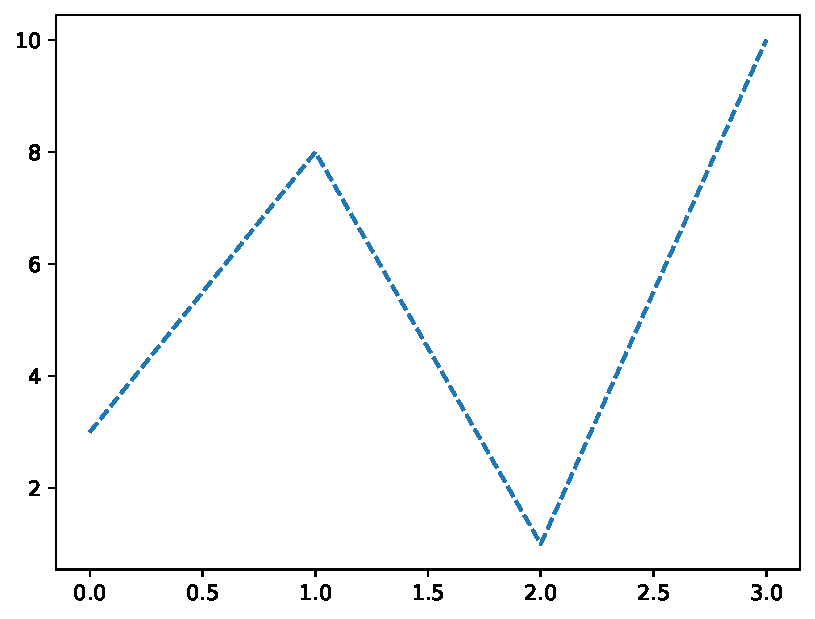
\includegraphics[scale=0.6]{img/grafica1017.pdf}
\end{figure}

\end{code}

\subsection{Sintaxis más corta}

El estilo de línea se puede escribir en una sintaxis más corta:

\begin{itemize}
  \item \texttt{linestyle} se puede escribir como \texttt{ls}.
  \item \texttt{dotted} se puede escribir como \texttt{:}.
  \item \texttt{dashed} se puede escribir como \texttt{-\/-}.
\end{itemize}

\begin{code} Sintaxis más corta.

\begin{Shaded}
\begin{Highlighting}[]
\NormalTok{plt.plot(ypoints, ls }\OperatorTok{=} \StringTok{\textquotesingle{}:\textquotesingle{}}\NormalTok{)}
\NormalTok{plt.show()}
\end{Highlighting}
\end{Shaded}

\begin{figure}
  \centering
  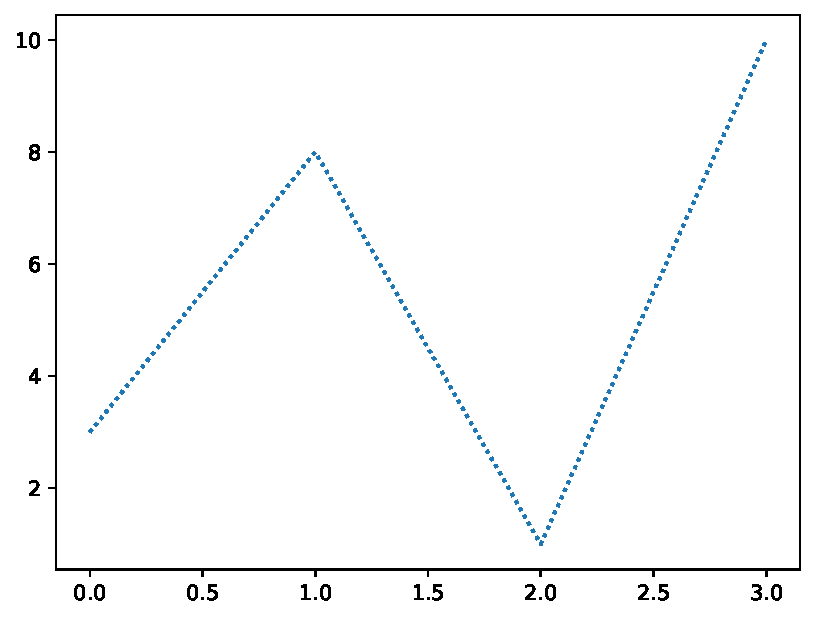
\includegraphics[scale=0.6]{img/grafica1018.pdf}
\end{figure}

\end{code}

\section{Estilos de Línea}

Puedes elegir cualquiera de estos estilos:

\textbar{} Style \textbar{} Or \textbar{}
\textbar:-....:\textbar:-\/-:\textbar{} \textbar{}
\textquotesingle solid\textquotesingle{} \textbar{} (default)
\textquotesingle-\textquotesingle{} \textbar{} \textbar{}
\textquotesingle dotted\textquotesingle{} \textbar{}
\textquotesingle:\textquotesingle{} \textbar{} \textbar{}
\textquotesingle dashed\textquotesingle{} \textbar{}
\textquotesingle-\/-\textquotesingle{} \textbar{} \textbar{}
\textquotesingle dashdot\textquotesingle{} \textbar{}
\textquotesingle-.\textquotesingle{} \textbar{} \textbar{}
\textquotesingle None\textquotesingle{} \textbar{}
\textquotesingle\textquotesingle{} or \textquotesingle{}
\textquotesingle{} \textbar{}

\section{Color de Línea}

Puede usar el argumento de palabra clave \texttt{color} o el más corto
\texttt{c} para establecer el color de la línea.

\begin{code} Establecer el color de la línea en rojo.

\begin{Shaded}
\begin{Highlighting}[]
\ImportTok{import}\NormalTok{ matplotlib.pyplot }\ImportTok{as}\NormalTok{ plt}
\ImportTok{import}\NormalTok{ numpy }\ImportTok{as}\NormalTok{ np}

\NormalTok{ypoints }\OperatorTok{=}\NormalTok{ np.array([}\DecValTok{3}\NormalTok{, }\DecValTok{8}\NormalTok{, }\DecValTok{1}\NormalTok{, }\DecValTok{10}\NormalTok{])}

\NormalTok{plt.plot(ypoints, color }\OperatorTok{=} \StringTok{\textquotesingle{}r\textquotesingle{}}\NormalTok{)}
\NormalTok{plt.show()}
\end{Highlighting}
\end{Shaded}

\begin{figure}
  \centering
  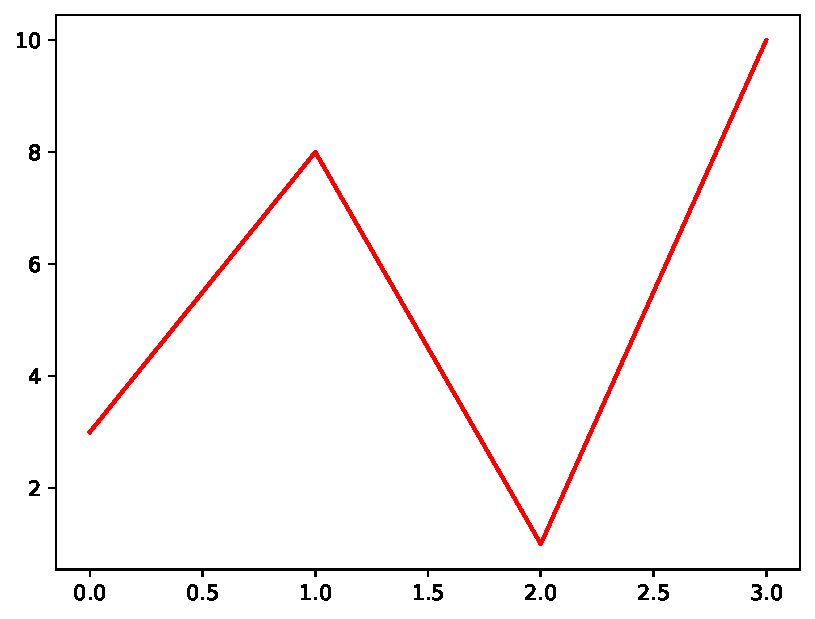
\includegraphics[scale=0.6]{img/grafica1019.pdf}
\end{figure}
\end{code}

También se puede utilizar el color en su valor hexadecimal o los nombres
de color compatibles.

\section{Ancho de Línea}

Puede usar el argumento de palabra clave \texttt{linewidth} o el más
corto \texttt{lw} para cambiar el ancho de la línea.

El valor es un número flotante, en puntos.

\begin{code} Parcela con una línea ancha de 20.5pt.

\begin{Shaded}
\begin{Highlighting}[]
\ImportTok{import}\NormalTok{ matplotlib.pyplot }\ImportTok{as}\NormalTok{ plt}
\ImportTok{import}\NormalTok{ numpy }\ImportTok{as}\NormalTok{ np}

\NormalTok{ypoints }\OperatorTok{=}\NormalTok{ np.array([}\DecValTok{3}\NormalTok{, }\DecValTok{8}\NormalTok{, }\DecValTok{1}\NormalTok{, }\DecValTok{10}\NormalTok{])}

\NormalTok{plt.plot(ypoints, linewidth }\OperatorTok{=} \StringTok{\textquotesingle{}20.5\textquotesingle{}}\NormalTok{)}
\NormalTok{plt.show()}
\end{Highlighting}
\end{Shaded}

\begin{figure}
  \centering
  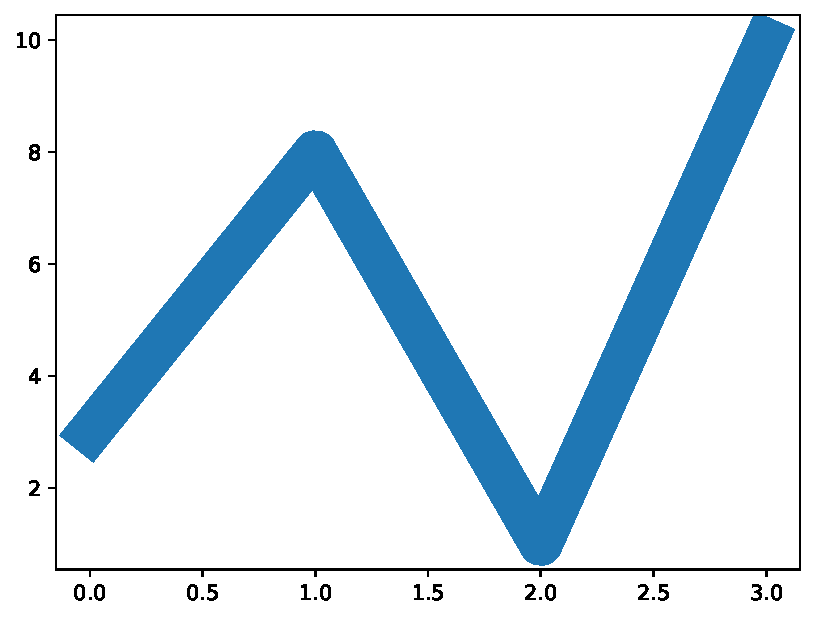
\includegraphics[scale=0.6]{img/grafica1020.pdf}
\end{figure}
\end{code}


\section{Múltiples Líneas}

Puede trazar tantas líneas como desee simplemente agregando más \texttt{plt.plot()} funciones.\\

\begin{code} Dibuja dos líneas especificando un \texttt{plt.plot()} función para cada línea.

\begin{Shaded}
\begin{Highlighting}[]
\ImportTok{import}\NormalTok{ matplotlib.pyplot }\ImportTok{as}\NormalTok{ plt}
\ImportTok{import}\NormalTok{ numpy }\ImportTok{as}\NormalTok{ np}

\NormalTok{y1 }\OperatorTok{=}\NormalTok{ np.array([}\DecValTok{3}\NormalTok{, }\DecValTok{8}\NormalTok{, }\DecValTok{1}\NormalTok{, }\DecValTok{10}\NormalTok{])}
\NormalTok{y2 }\OperatorTok{=}\NormalTok{ np.array([}\DecValTok{6}\NormalTok{, }\DecValTok{2}\NormalTok{, }\DecValTok{7}\NormalTok{, }\DecValTok{11}\NormalTok{])}

\NormalTok{plt.plot(y1)}
\NormalTok{plt.plot(y2)}

\NormalTok{plt.show()}
\end{Highlighting}
\end{Shaded}

\begin{figure}
  \centering
  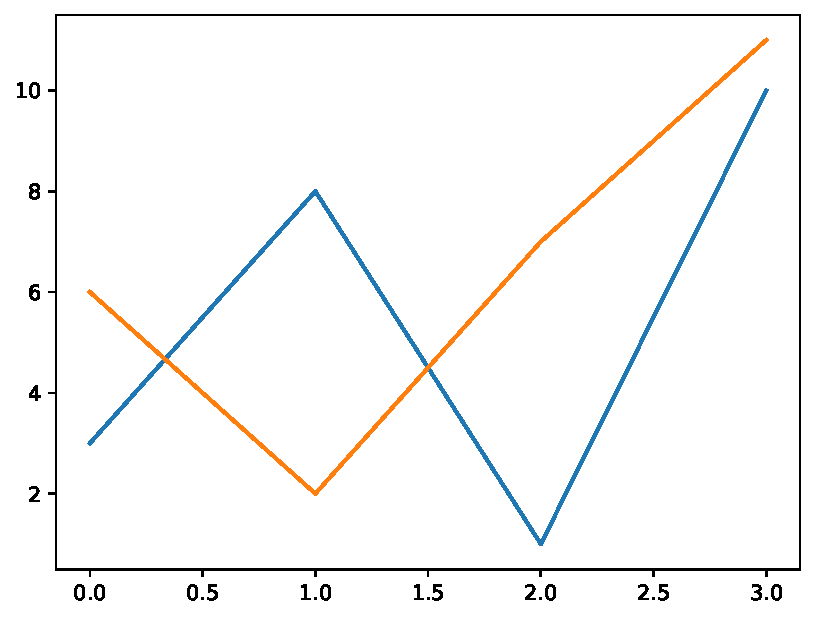
\includegraphics[scale=0.6]{img/grafica1021.pdf}
\end{figure}
\end{code}

También puede trazar muchas líneas agregando los puntos para el eje
\(x\) y \(y\) para cada línea en la misma función \texttt{plt.plot()}.

(En los ejemplos anteriores solo especificamos los puntos en el eje y,
lo que significa que los puntos en el eje x obtuvieron los valores
predeterminados (0, 1, 2, 3).)

Los valores \(x\) y \(y\) vienen en pares.\\

\begin{code} Dibuje dos líneas especificando los valores \(x\) y \(y\) para ambas líneas.

\begin{Shaded}
\begin{Highlighting}[]
\ImportTok{import}\NormalTok{ matplotlib.pyplot }\ImportTok{as}\NormalTok{ plt}
\ImportTok{import}\NormalTok{ numpy }\ImportTok{as}\NormalTok{ np}

\NormalTok{x1 }\OperatorTok{=}\NormalTok{ np.array([}\DecValTok{0}\NormalTok{, }\DecValTok{1}\NormalTok{, }\DecValTok{2}\NormalTok{, }\DecValTok{3}\NormalTok{])}
\NormalTok{y1 }\OperatorTok{=}\NormalTok{ np.array([}\DecValTok{3}\NormalTok{, }\DecValTok{8}\NormalTok{, }\DecValTok{1}\NormalTok{, }\DecValTok{10}\NormalTok{])}
\NormalTok{x2 }\OperatorTok{=}\NormalTok{ np.array([}\DecValTok{0}\NormalTok{, }\DecValTok{1}\NormalTok{, }\DecValTok{2}\NormalTok{, }\DecValTok{3}\NormalTok{])}
\NormalTok{y2 }\OperatorTok{=}\NormalTok{ np.array([}\DecValTok{6}\NormalTok{, }\DecValTok{2}\NormalTok{, }\DecValTok{7}\NormalTok{, }\DecValTok{11}\NormalTok{])}

\NormalTok{plt.plot(x1, y1, x2, y2)}
\NormalTok{plt.show()}
\end{Highlighting}
\end{Shaded}

\begin{figure}
  \centering
  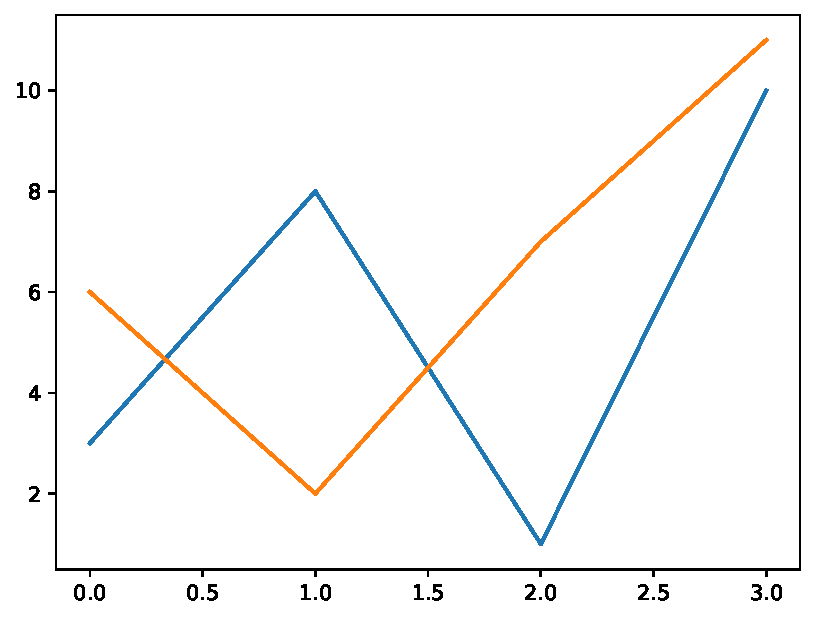
\includegraphics[scale=0.6]{img/grafica1022.pdf}
\end{figure}

\end{code}

\section{Crear Etiquetas para una gráfica}

Con \texttt{Pyplot}, puede usar las funciones \texttt{xlabel()} y
\texttt{ylabel()} para establecer una etiqueta para el eje \(x\) y
\(y\).

\begin{code} Agregar etiquetas al eje \(x\) y \(y\).

\begin{Shaded}
\begin{Highlighting}[]
\ImportTok{import}\NormalTok{ numpy }\ImportTok{as}\NormalTok{ np}
\ImportTok{import}\NormalTok{ matplotlib.pyplot }\ImportTok{as}\NormalTok{ plt}

\NormalTok{x }\OperatorTok{=}\NormalTok{ np.array([}\DecValTok{80}\NormalTok{, }\DecValTok{85}\NormalTok{, }\DecValTok{90}\NormalTok{, }\DecValTok{95}\NormalTok{, }\DecValTok{100}\NormalTok{, }\DecValTok{105}\NormalTok{, }\DecValTok{110}\NormalTok{, }\DecValTok{115}\NormalTok{, }\DecValTok{120}\NormalTok{, }\DecValTok{125}\NormalTok{])}
\NormalTok{y }\OperatorTok{=}\NormalTok{ np.array([}\DecValTok{240}\NormalTok{, }\DecValTok{250}\NormalTok{, }\DecValTok{260}\NormalTok{, }\DecValTok{270}\NormalTok{, }\DecValTok{280}\NormalTok{, }\DecValTok{290}\NormalTok{, }\DecValTok{300}\NormalTok{, }\DecValTok{310}\NormalTok{, }\DecValTok{320}\NormalTok{, }\DecValTok{330}\NormalTok{])}

\NormalTok{plt.plot(x, y)}

\NormalTok{plt.xlabel(}\StringTok{"Average Pulse"}\NormalTok{)}
\NormalTok{plt.ylabel(}\StringTok{"Calorie Burnage"}\NormalTok{)}

\NormalTok{plt.show()}
\end{Highlighting}
\end{Shaded}

\begin{figure}
  \centering
  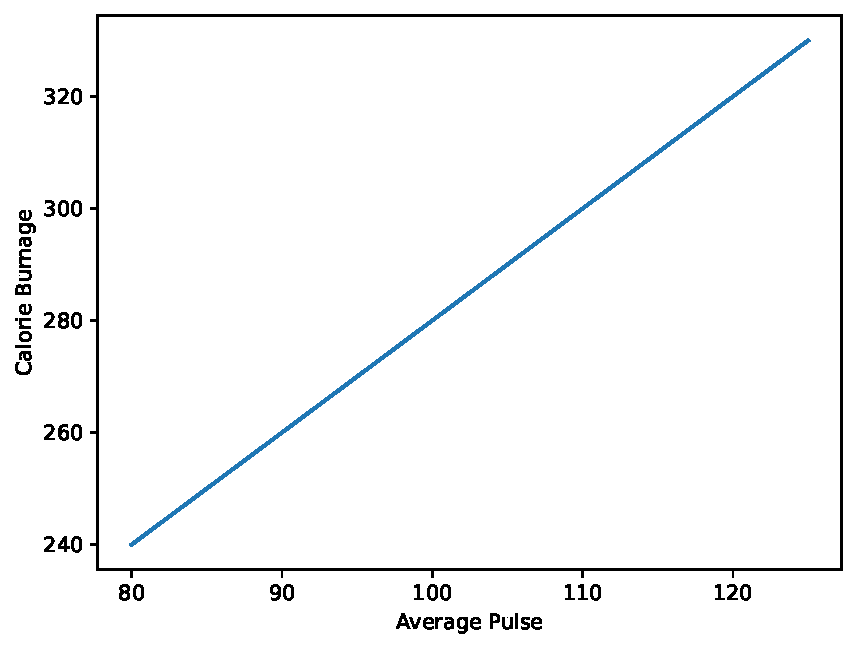
\includegraphics[scale=0.6]{img/grafica1023.pdf}
\end{figure}
\end{code}

\section{Crear un título para una trama}

Con \texttt{Pyplot}, puedes utilizar la función \texttt{title()} para
establecer un título para el gráfico.

\begin{code} Agregue un título de gráfico y etiquetas para los ejes x e y.

\begin{Shaded}
\begin{Highlighting}[]
\ImportTok{import}\NormalTok{ numpy }\ImportTok{as}\NormalTok{ np}
\ImportTok{import}\NormalTok{ matplotlib.pyplot }\ImportTok{as}\NormalTok{ plt}

\NormalTok{x }\OperatorTok{=}\NormalTok{ np.array([}\DecValTok{80}\NormalTok{, }\DecValTok{85}\NormalTok{, }\DecValTok{90}\NormalTok{, }\DecValTok{95}\NormalTok{, }\DecValTok{100}\NormalTok{, }\DecValTok{105}\NormalTok{, }\DecValTok{110}\NormalTok{, }\DecValTok{115}\NormalTok{, }\DecValTok{120}\NormalTok{, }\DecValTok{125}\NormalTok{])}
\NormalTok{y }\OperatorTok{=}\NormalTok{ np.array([}\DecValTok{240}\NormalTok{, }\DecValTok{250}\NormalTok{, }\DecValTok{260}\NormalTok{, }\DecValTok{270}\NormalTok{, }\DecValTok{280}\NormalTok{, }\DecValTok{290}\NormalTok{, }\DecValTok{300}\NormalTok{, }\DecValTok{310}\NormalTok{, }\DecValTok{320}\NormalTok{, }\DecValTok{330}\NormalTok{])}

\NormalTok{plt.plot(x, y)}

\NormalTok{plt.title(}\StringTok{"Sports Watch Data"}\NormalTok{)}
\NormalTok{plt.xlabel(}\StringTok{"Average Pulse"}\NormalTok{)}
\NormalTok{plt.ylabel(}\StringTok{"Calorie Burnage"}\NormalTok{)}

\NormalTok{plt.show()}
\end{Highlighting}
\end{Shaded}

\begin{figure}
  \centering
  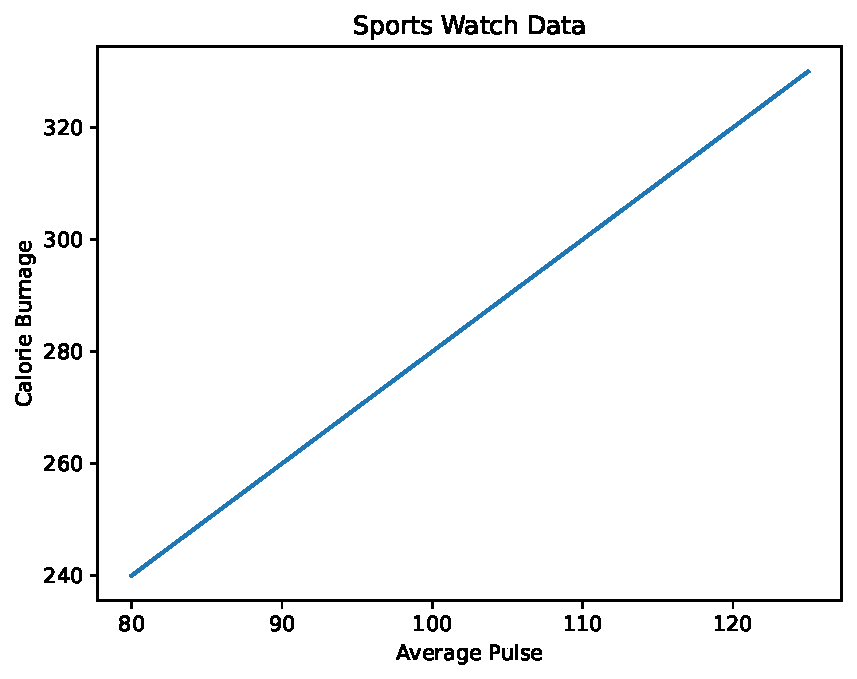
\includegraphics[scale=0.6]{img/grafica1024.pdf}
\end{figure}
\end{code}

\section{Establecer fuente para títulos y etiquetas}

Puede utilizar el parámetro \texttt{fontdict} en \texttt{xlabel()},
\texttt{ylabel()} y \texttt{title()} para establecer las propiedades de
fuente para el título y las etiquetas.

\begin{code} Establecer propiedades de fuente para el título y las etiquetas.

\begin{Shaded}
\begin{Highlighting}[]
\ImportTok{import}\NormalTok{ numpy }\ImportTok{as}\NormalTok{ np}
\ImportTok{import}\NormalTok{ matplotlib.pyplot }\ImportTok{as}\NormalTok{ plt}

\NormalTok{x }\OperatorTok{=}\NormalTok{ np.array([}\DecValTok{80}\NormalTok{, }\DecValTok{85}\NormalTok{, }\DecValTok{90}\NormalTok{, }\DecValTok{95}\NormalTok{, }\DecValTok{100}\NormalTok{, }\DecValTok{105}\NormalTok{, }\DecValTok{110}\NormalTok{, }\DecValTok{115}\NormalTok{, }\DecValTok{120}\NormalTok{, }\DecValTok{125}\NormalTok{])}
\NormalTok{y }\OperatorTok{=}\NormalTok{ np.array([}\DecValTok{240}\NormalTok{, }\DecValTok{250}\NormalTok{, }\DecValTok{260}\NormalTok{, }\DecValTok{270}\NormalTok{, }\DecValTok{280}\NormalTok{, }\DecValTok{290}\NormalTok{, }\DecValTok{300}\NormalTok{, }\DecValTok{310}\NormalTok{, }\DecValTok{320}\NormalTok{, }\DecValTok{330}\NormalTok{])}

\NormalTok{font1 }\OperatorTok{=}\NormalTok{ \{}\StringTok{\textquotesingle{}family\textquotesingle{}}\NormalTok{:}\StringTok{\textquotesingle{}serif\textquotesingle{}}\NormalTok{,}\StringTok{\textquotesingle{}color\textquotesingle{}}\NormalTok{:}\StringTok{\textquotesingle{}blue\textquotesingle{}}\NormalTok{,}\StringTok{\textquotesingle{}size\textquotesingle{}}\NormalTok{:}\DecValTok{20}\NormalTok{\}}
\NormalTok{font2 }\OperatorTok{=}\NormalTok{ \{}\StringTok{\textquotesingle{}family\textquotesingle{}}\NormalTok{:}\StringTok{\textquotesingle{}serif\textquotesingle{}}\NormalTok{,}\StringTok{\textquotesingle{}color\textquotesingle{}}\NormalTok{:}\StringTok{\textquotesingle{}darkred\textquotesingle{}}\NormalTok{,}\StringTok{\textquotesingle{}size\textquotesingle{}}\NormalTok{:}\DecValTok{15}\NormalTok{\}}

\NormalTok{plt.title(}\StringTok{"Sports Watch Data"}\NormalTok{, fontdict }\OperatorTok{=}\NormalTok{ font1)}
\NormalTok{plt.xlabel(}\StringTok{"Average Pulse"}\NormalTok{, fontdict }\OperatorTok{=}\NormalTok{ font2)}
\NormalTok{plt.ylabel(}\StringTok{"Calorie Burnage"}\NormalTok{, fontdict }\OperatorTok{=}\NormalTok{ font2)}

\NormalTok{plt.plot(x, y)}
\NormalTok{plt.show()}
\end{Highlighting}
\end{Shaded}

\begin{figure}
  \centering
  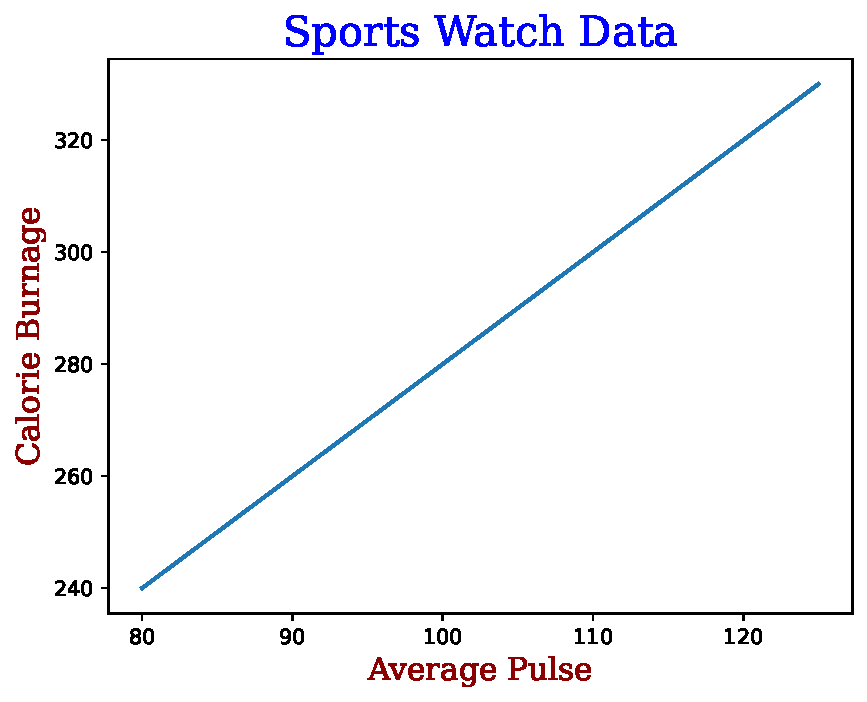
\includegraphics[scale=0.6]{img/grafica1025.pdf}
\end{figure}
\end{code}

\section{Posicionar el título}

Puedes utilizar el parámetro \texttt{loc} en \texttt{title()} para
posicionar el título.

Los valores admitidos son:
\emph{\textquotesingle left\textquotesingle{}},
\emph{\textquotesingle right\textquotesingle{}} y
\emph{\textquotesingle center\textquotesingle{}}. El valor
predeterminado es \emph{\textquotesingle center\textquotesingle{}}.

\begin{code} Coloque el título a la izquierda.

\begin{Shaded}
\begin{Highlighting}[]
\ImportTok{import}\NormalTok{ numpy }\ImportTok{as}\NormalTok{ np}
\ImportTok{import}\NormalTok{ matplotlib.pyplot }\ImportTok{as}\NormalTok{ plt}

\NormalTok{x }\OperatorTok{=}\NormalTok{ np.array([}\DecValTok{80}\NormalTok{, }\DecValTok{85}\NormalTok{, }\DecValTok{90}\NormalTok{, }\DecValTok{95}\NormalTok{, }\DecValTok{100}\NormalTok{, }\DecValTok{105}\NormalTok{, }\DecValTok{110}\NormalTok{, }\DecValTok{115}\NormalTok{, }\DecValTok{120}\NormalTok{, }\DecValTok{125}\NormalTok{])}
\NormalTok{y }\OperatorTok{=}\NormalTok{ np.array([}\DecValTok{240}\NormalTok{, }\DecValTok{250}\NormalTok{, }\DecValTok{260}\NormalTok{, }\DecValTok{270}\NormalTok{, }\DecValTok{280}\NormalTok{, }\DecValTok{290}\NormalTok{, }\DecValTok{300}\NormalTok{, }\DecValTok{310}\NormalTok{, }\DecValTok{320}\NormalTok{, }\DecValTok{330}\NormalTok{])}

\NormalTok{plt.title(}\StringTok{"Sports Watch Data"}\NormalTok{, loc }\OperatorTok{=} \StringTok{\textquotesingle{}left\textquotesingle{}}\NormalTok{)}
\NormalTok{plt.xlabel(}\StringTok{"Average Pulse"}\NormalTok{)}
\NormalTok{plt.ylabel(}\StringTok{"Calorie Burnage"}\NormalTok{)}

\NormalTok{plt.plot(x, y)}
\NormalTok{plt.show()}
\end{Highlighting}
\end{Shaded}

\begin{figure}
  \centering
  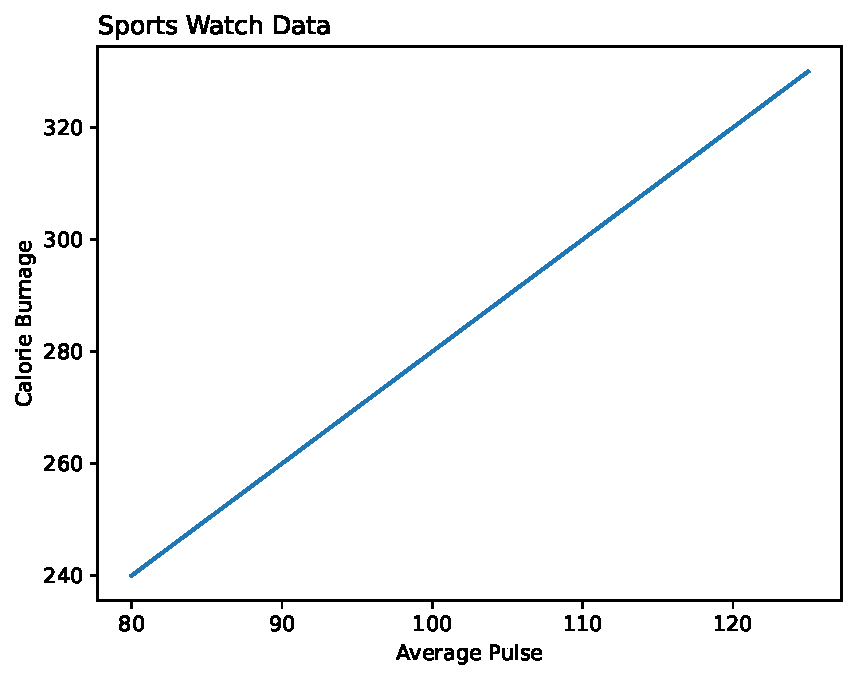
\includegraphics[scale=0.6]{img/grafica1026.pdf}
\end{figure}
\end{code}


\section{Agregar cuadrícula a un gráfico}

Con \texttt{Pyplot}, puedes usar la función \texttt{grid()} para agregar
cuadrícula al gráfico.

\begin{code} Añadir líneas de cuadrícula al gráfico.

\begin{Shaded}
\begin{Highlighting}[]
\ImportTok{import}\NormalTok{ numpy }\ImportTok{as}\NormalTok{ np}
\ImportTok{import}\NormalTok{ matplotlib.pyplot }\ImportTok{as}\NormalTok{ plt}

\NormalTok{x }\OperatorTok{=}\NormalTok{ np.array([}\DecValTok{80}\NormalTok{, }\DecValTok{85}\NormalTok{, }\DecValTok{90}\NormalTok{, }\DecValTok{95}\NormalTok{, }\DecValTok{100}\NormalTok{, }\DecValTok{105}\NormalTok{, }\DecValTok{110}\NormalTok{, }\DecValTok{115}\NormalTok{, }\DecValTok{120}\NormalTok{, }\DecValTok{125}\NormalTok{])}
\NormalTok{y }\OperatorTok{=}\NormalTok{ np.array([}\DecValTok{240}\NormalTok{, }\DecValTok{250}\NormalTok{, }\DecValTok{260}\NormalTok{, }\DecValTok{270}\NormalTok{, }\DecValTok{280}\NormalTok{, }\DecValTok{290}\NormalTok{, }\DecValTok{300}\NormalTok{, }\DecValTok{310}\NormalTok{, }\DecValTok{320}\NormalTok{, }\DecValTok{330}\NormalTok{])}

\NormalTok{plt.title(}\StringTok{"Sports Watch Data"}\NormalTok{)}
\NormalTok{plt.xlabel(}\StringTok{"Average Pulse"}\NormalTok{)}
\NormalTok{plt.ylabel(}\StringTok{"Calorie Burnage"}\NormalTok{)}

\NormalTok{plt.plot(x, y)}
\NormalTok{plt.grid()}
\NormalTok{plt.show()}
\end{Highlighting}
\end{Shaded}

\begin{figure}
  \centering
  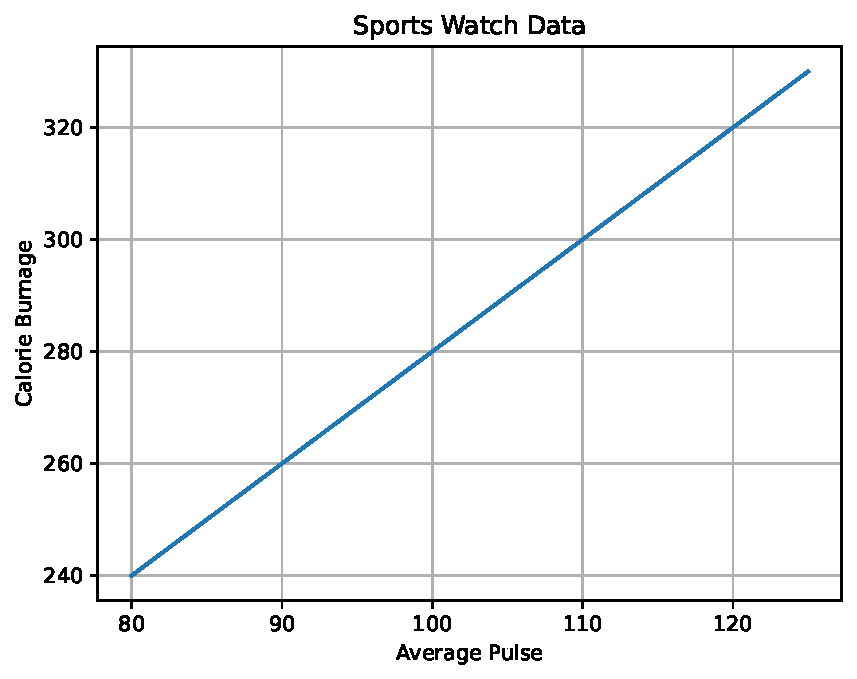
\includegraphics[scale=0.6]{img/grafica1027.pdf}
\end{figure}

\end{code}


\section{Especificar qué líneas de cuadrícula se mostrarán}

Puede utilizar el parámetro \texttt{axis} en la función \texttt{grid()}
para especificar qué líneas de cuadrícula mostrar.

Los valores admitidos son: \emph{\textquotesingle x\textquotesingle{}},
\emph{\textquotesingle y\textquotesingle{}} y
\emph{\textquotesingle both\textquotesingle{}}. El valor predeterminado
es \emph{\textquotesingle both\textquotesingle{}}.

\begin{code} Mostrar solo líneas de cuadrícula para el eje \(x\).

\begin{Shaded}
\begin{Highlighting}[]
\ImportTok{import}\NormalTok{ numpy }\ImportTok{as}\NormalTok{ np}
\ImportTok{import}\NormalTok{ matplotlib.pyplot }\ImportTok{as}\NormalTok{ plt}

\NormalTok{x }\OperatorTok{=}\NormalTok{ np.array([}\DecValTok{80}\NormalTok{, }\DecValTok{85}\NormalTok{, }\DecValTok{90}\NormalTok{, }\DecValTok{95}\NormalTok{, }\DecValTok{100}\NormalTok{, }\DecValTok{105}\NormalTok{, }\DecValTok{110}\NormalTok{, }\DecValTok{115}\NormalTok{, }\DecValTok{120}\NormalTok{, }\DecValTok{125}\NormalTok{])}
\NormalTok{y }\OperatorTok{=}\NormalTok{ np.array([}\DecValTok{240}\NormalTok{, }\DecValTok{250}\NormalTok{, }\DecValTok{260}\NormalTok{, }\DecValTok{270}\NormalTok{, }\DecValTok{280}\NormalTok{, }\DecValTok{290}\NormalTok{, }\DecValTok{300}\NormalTok{, }\DecValTok{310}\NormalTok{, }\DecValTok{320}\NormalTok{, }\DecValTok{330}\NormalTok{])}

\NormalTok{plt.title(}\StringTok{"Sports Watch Data"}\NormalTok{)}
\NormalTok{plt.xlabel(}\StringTok{"Average Pulse"}\NormalTok{)}
\NormalTok{plt.ylabel(}\StringTok{"Calorie Burnage"}\NormalTok{)}

\NormalTok{plt.plot(x, y)}
\NormalTok{plt.grid(axis }\OperatorTok{=} \StringTok{\textquotesingle{}x\textquotesingle{}}\NormalTok{)}
\NormalTok{plt.show()}
\end{Highlighting}
\end{Shaded}

\begin{figure}
  \centering
  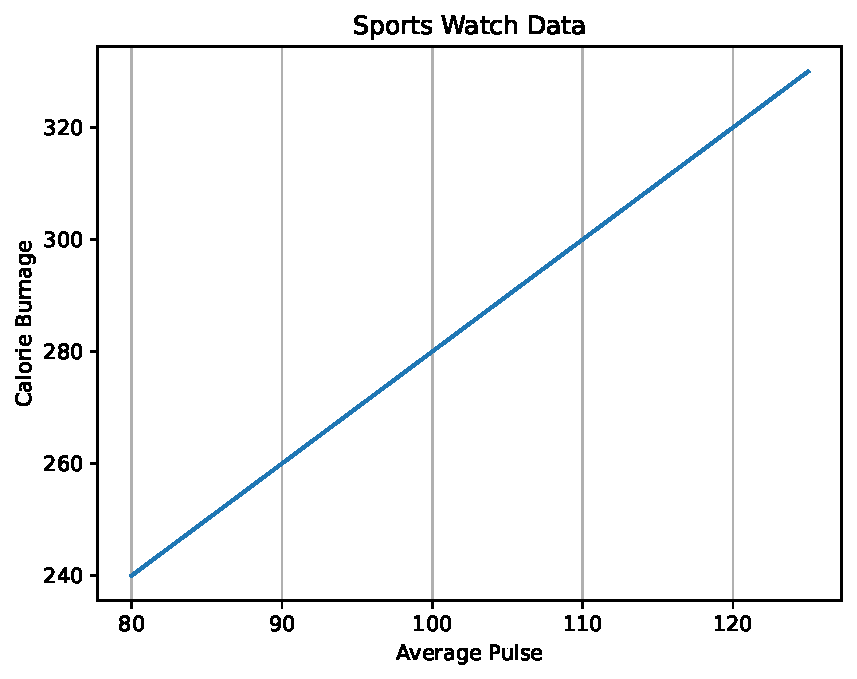
\includegraphics[scale=0.6]{img/grafica1028.pdf}
\end{figure}
\end{code}


\begin{code} Mostrar solo líneas de cuadrícula para el eje \(y\).

\begin{Shaded}
\begin{Highlighting}[]
\ImportTok{import}\NormalTok{ numpy }\ImportTok{as}\NormalTok{ np}
\ImportTok{import}\NormalTok{ matplotlib.pyplot }\ImportTok{as}\NormalTok{ plt}

\NormalTok{x }\OperatorTok{=}\NormalTok{ np.array([}\DecValTok{80}\NormalTok{, }\DecValTok{85}\NormalTok{, }\DecValTok{90}\NormalTok{, }\DecValTok{95}\NormalTok{, }\DecValTok{100}\NormalTok{, }\DecValTok{105}\NormalTok{, }\DecValTok{110}\NormalTok{, }\DecValTok{115}\NormalTok{, }\DecValTok{120}\NormalTok{, }\DecValTok{125}\NormalTok{])}
\NormalTok{y }\OperatorTok{=}\NormalTok{ np.array([}\DecValTok{240}\NormalTok{, }\DecValTok{250}\NormalTok{, }\DecValTok{260}\NormalTok{, }\DecValTok{270}\NormalTok{, }\DecValTok{280}\NormalTok{, }\DecValTok{290}\NormalTok{, }\DecValTok{300}\NormalTok{, }\DecValTok{310}\NormalTok{, }\DecValTok{320}\NormalTok{, }\DecValTok{330}\NormalTok{])}

\NormalTok{plt.title(}\StringTok{"Sports Watch Data"}\NormalTok{)}
\NormalTok{plt.xlabel(}\StringTok{"Average Pulse"}\NormalTok{)}
\NormalTok{plt.ylabel(}\StringTok{"Calorie Burnage"}\NormalTok{)}

\NormalTok{plt.plot(x, y)}
\NormalTok{plt.grid(axis }\OperatorTok{=} \StringTok{\textquotesingle{}y\textquotesingle{}}\NormalTok{)}
\NormalTok{plt.show()}
\end{Highlighting}
\end{Shaded}

\begin{figure}
  \centering
  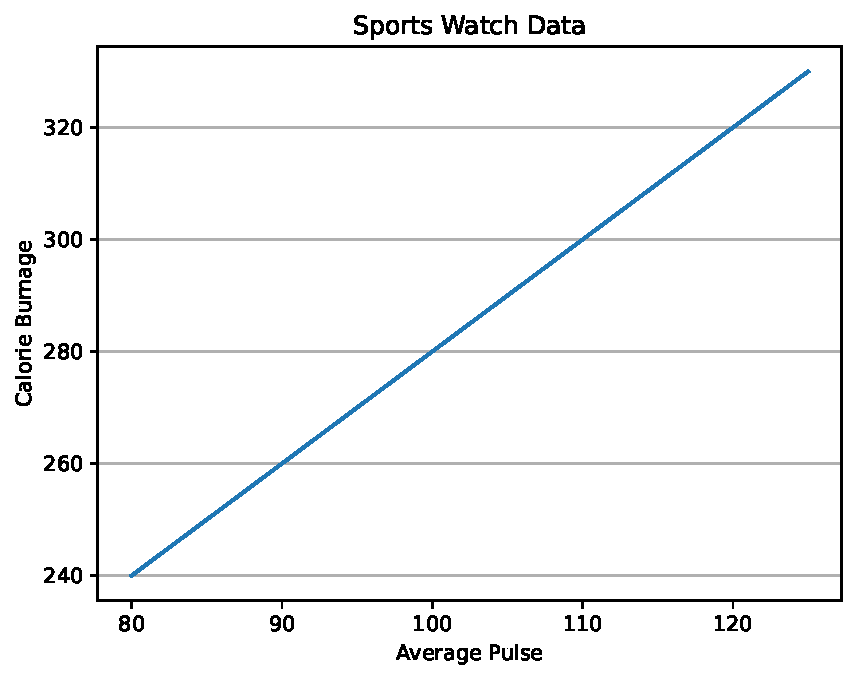
\includegraphics[scale=0.6]{img/grafica1029.pdf}
\end{figure}
\end{code}

\section{Establecer propiedades de línea para la cuadrícula}

También puede configurar las propiedades de línea de la cuadrícula, de esta manera:
\texttt{grid(color\ =\ \textquotesingle{}\_color\_\textquotesingle{},\ linestyle\ =\ \textquotesingle{}\_linestyle\_\textquotesingle{},\ linewidth\ =\ \_number\_)}.

\begin{code} Establecer las propiedades de línea de la cuadrícula.

\begin{Shaded}
\begin{Highlighting}[]
\ImportTok{import}\NormalTok{ numpy }\ImportTok{as}\NormalTok{ np}
\ImportTok{import}\NormalTok{ matplotlib.pyplot }\ImportTok{as}\NormalTok{ plt}

\NormalTok{x }\OperatorTok{=}\NormalTok{ np.array([}\DecValTok{80}\NormalTok{, }\DecValTok{85}\NormalTok{, }\DecValTok{90}\NormalTok{, }\DecValTok{95}\NormalTok{, }\DecValTok{100}\NormalTok{, }\DecValTok{105}\NormalTok{, }\DecValTok{110}\NormalTok{, }\DecValTok{115}\NormalTok{, }\DecValTok{120}\NormalTok{, }\DecValTok{125}\NormalTok{])}
\NormalTok{y }\OperatorTok{=}\NormalTok{ np.array([}\DecValTok{240}\NormalTok{, }\DecValTok{250}\NormalTok{, }\DecValTok{260}\NormalTok{, }\DecValTok{270}\NormalTok{, }\DecValTok{280}\NormalTok{, }\DecValTok{290}\NormalTok{, }\DecValTok{300}\NormalTok{, }\DecValTok{310}\NormalTok{, }\DecValTok{320}\NormalTok{, }\DecValTok{330}\NormalTok{])}

\NormalTok{plt.title(}\StringTok{"Sports Watch Data"}\NormalTok{)}
\NormalTok{plt.xlabel(}\StringTok{"Average Pulse"}\NormalTok{)}
\NormalTok{plt.ylabel(}\StringTok{"Calorie Burnage"}\NormalTok{)}

\NormalTok{plt.plot(x, y)}
\NormalTok{plt.grid(color }\OperatorTok{=} \StringTok{\textquotesingle{}green\textquotesingle{}}\NormalTok{, linestyle }\OperatorTok{=} \StringTok{\textquotesingle{}{-}{-}\textquotesingle{}}\NormalTok{, linewidth }\OperatorTok{=} \FloatTok{0.5}\NormalTok{)}
\NormalTok{plt.show()}
\end{Highlighting}
\end{Shaded}

\begin{figure}
  \centering
  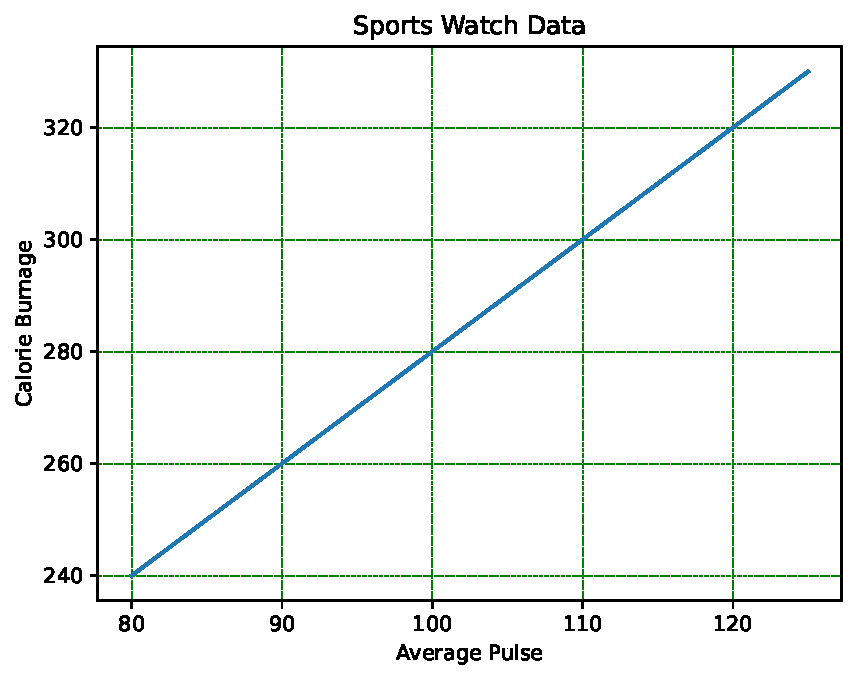
\includegraphics[scale=0.6]{img/grafica1030.pdf}
\end{figure}
\end{code}

\section{Mostrar múltiples gráficos}

Con esta función \texttt{subplot()} puedes dibujar múltiples gráficos en
una figura.

\begin{code} Dibuje 2 gráficos.

\begin{Shaded}
\begin{Highlighting}[]
\ImportTok{import}\NormalTok{ matplotlib.pyplot }\ImportTok{as}\NormalTok{ plt}
\ImportTok{import}\NormalTok{ numpy }\ImportTok{as}\NormalTok{ np}

\CommentTok{\#plot 1:}
\NormalTok{x }\OperatorTok{=}\NormalTok{ np.array([}\DecValTok{0}\NormalTok{, }\DecValTok{1}\NormalTok{, }\DecValTok{2}\NormalTok{, }\DecValTok{3}\NormalTok{])}
\NormalTok{y }\OperatorTok{=}\NormalTok{ np.array([}\DecValTok{3}\NormalTok{, }\DecValTok{8}\NormalTok{, }\DecValTok{1}\NormalTok{, }\DecValTok{10}\NormalTok{])}

\NormalTok{plt.subplot(}\DecValTok{1}\NormalTok{, }\DecValTok{2}\NormalTok{, }\DecValTok{1}\NormalTok{)}
\NormalTok{plt.plot(x,y)}

\CommentTok{\#plot 2:}
\NormalTok{x }\OperatorTok{=}\NormalTok{ np.array([}\DecValTok{0}\NormalTok{, }\DecValTok{1}\NormalTok{, }\DecValTok{2}\NormalTok{, }\DecValTok{3}\NormalTok{])}
\NormalTok{y }\OperatorTok{=}\NormalTok{ np.array([}\DecValTok{10}\NormalTok{, }\DecValTok{20}\NormalTok{, }\DecValTok{30}\NormalTok{, }\DecValTok{40}\NormalTok{])}

\NormalTok{plt.subplot(}\DecValTok{1}\NormalTok{, }\DecValTok{2}\NormalTok{, }\DecValTok{2}\NormalTok{)}
\NormalTok{plt.plot(x,y)}
\NormalTok{plt.show()}
\end{Highlighting}
\end{Shaded}

\begin{figure}
  \centering
  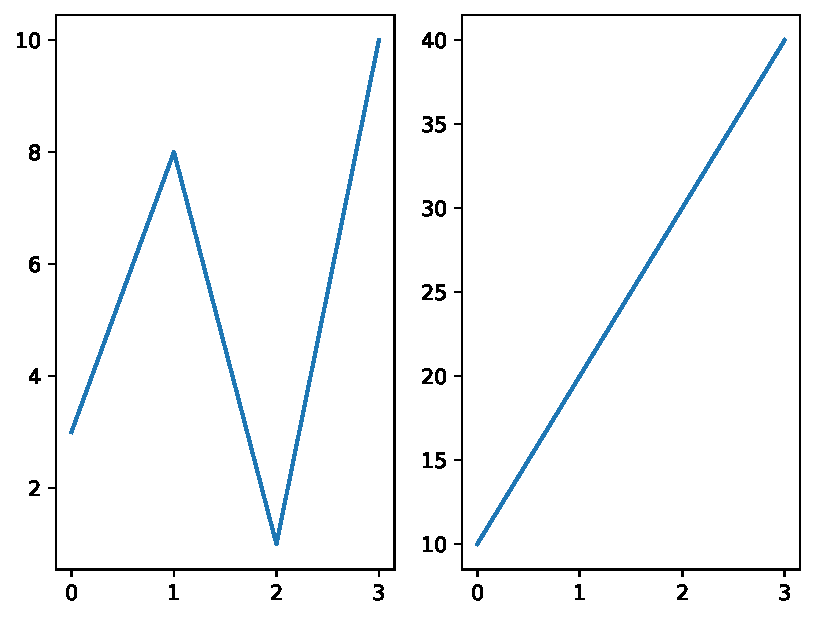
\includegraphics[scale=0.6]{img/grafica1031.pdf}
\end{figure}
\end{code}

\section{La función subplot()}

La función \texttt{subplot()} toma tres argumentos que describen el
diseño de la figura.

El diseño está organizado en filas y columnas, que están representadas
por el primer y segundo argumento.

El tercer argumento representa el índice de la malla actual.

\begin{Shaded}
\begin{Highlighting}[]
\NormalTok{plt.subplot(}\DecValTok{1}\NormalTok{, }\DecValTok{2}\NormalTok{, }\DecValTok{1}\NormalTok{)}
\CommentTok{\#the figure has 1 row, 2 columns, and this plot is the first plot.}
\end{Highlighting}
\end{Shaded}

\begin{Shaded}
\begin{Highlighting}[]
\NormalTok{plt.subplot(}\DecValTok{1}\NormalTok{, }\DecValTok{2}\NormalTok{, }\DecValTok{2}\NormalTok{)}
\CommentTok{\#the figure has 1 row, 2 columns, and this plot is the second plot.}
\end{Highlighting}
\end{Shaded}

Entonces, si queremos una figura con 2 filas y 1 columna (lo que
significa que los dos gráficos se mostrarán uno encima del otro en lugar
de uno al lado del otro), podemos escribir la sintaxis de esta manera.

\begin{code} Dibuje 2 gráficos uno encima del otro.

\begin{Shaded}
\begin{Highlighting}[]
\ImportTok{import}\NormalTok{ matplotlib.pyplot }\ImportTok{as}\NormalTok{ plt}
\ImportTok{import}\NormalTok{ numpy }\ImportTok{as}\NormalTok{ np}

\CommentTok{\#plot 1:}
\NormalTok{x }\OperatorTok{=}\NormalTok{ np.array([}\DecValTok{0}\NormalTok{, }\DecValTok{1}\NormalTok{, }\DecValTok{2}\NormalTok{, }\DecValTok{3}\NormalTok{])}
\NormalTok{y }\OperatorTok{=}\NormalTok{ np.array([}\DecValTok{3}\NormalTok{, }\DecValTok{8}\NormalTok{, }\DecValTok{1}\NormalTok{, }\DecValTok{10}\NormalTok{])}

\NormalTok{plt.subplot(}\DecValTok{2}\NormalTok{, }\DecValTok{1}\NormalTok{, }\DecValTok{1}\NormalTok{)}
\NormalTok{plt.plot(x,y)}

\CommentTok{\#plot 2:}
\NormalTok{x }\OperatorTok{=}\NormalTok{ np.array([}\DecValTok{0}\NormalTok{, }\DecValTok{1}\NormalTok{, }\DecValTok{2}\NormalTok{, }\DecValTok{3}\NormalTok{])}
\NormalTok{y }\OperatorTok{=}\NormalTok{ np.array([}\DecValTok{10}\NormalTok{, }\DecValTok{20}\NormalTok{, }\DecValTok{30}\NormalTok{, }\DecValTok{40}\NormalTok{])}

\NormalTok{plt.subplot(}\DecValTok{2}\NormalTok{, }\DecValTok{1}\NormalTok{, }\DecValTok{2}\NormalTok{)}
\NormalTok{plt.plot(x,y)}
\NormalTok{plt.show()}
\end{Highlighting}
\end{Shaded}

\begin{figure}
  \centering
  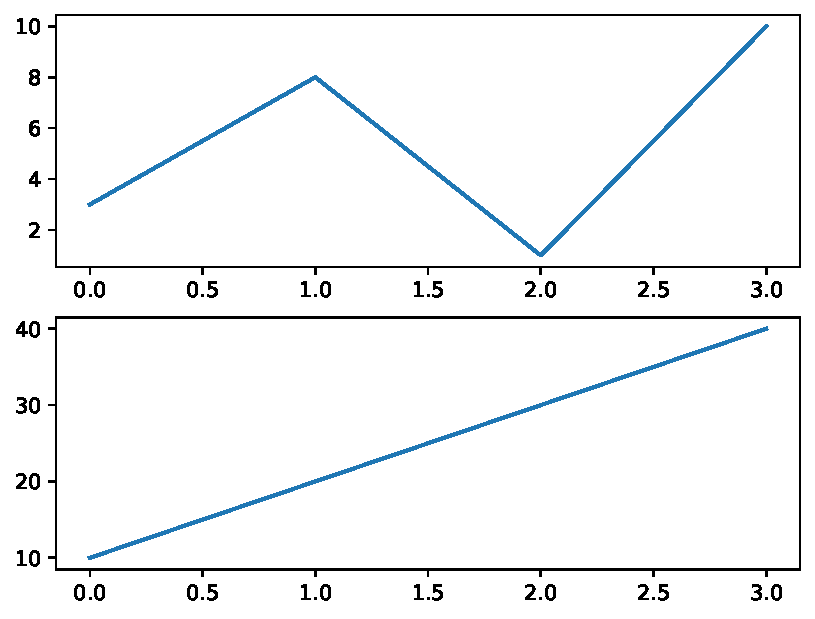
\includegraphics[scale=0.6]{img/grafica1032.pdf}
\end{figure}
\end{code}

Puede dibujar tantos gráficos como quiera en una figura, simplemente
describa el número de filas, columnas y el índice del gráfico.

\begin{code} Dibuje 6 gráficos.

\begin{Shaded}
\begin{Highlighting}[]
\ImportTok{import}\NormalTok{ matplotlib.pyplot }\ImportTok{as}\NormalTok{ plt}
\ImportTok{import}\NormalTok{ numpy }\ImportTok{as}\NormalTok{ np}

\NormalTok{x }\OperatorTok{=}\NormalTok{ np.array([}\DecValTok{0}\NormalTok{, }\DecValTok{1}\NormalTok{, }\DecValTok{2}\NormalTok{, }\DecValTok{3}\NormalTok{])}
\NormalTok{y }\OperatorTok{=}\NormalTok{ np.array([}\DecValTok{3}\NormalTok{, }\DecValTok{8}\NormalTok{, }\DecValTok{1}\NormalTok{, }\DecValTok{10}\NormalTok{])}

\NormalTok{plt.subplot(}\DecValTok{2}\NormalTok{, }\DecValTok{3}\NormalTok{, }\DecValTok{1}\NormalTok{)}
\NormalTok{plt.plot(x,y)}

\NormalTok{x }\OperatorTok{=}\NormalTok{ np.array([}\DecValTok{0}\NormalTok{, }\DecValTok{1}\NormalTok{, }\DecValTok{2}\NormalTok{, }\DecValTok{3}\NormalTok{])}
\NormalTok{y }\OperatorTok{=}\NormalTok{ np.array([}\DecValTok{10}\NormalTok{, }\DecValTok{20}\NormalTok{, }\DecValTok{30}\NormalTok{, }\DecValTok{40}\NormalTok{])}

\NormalTok{plt.subplot(}\DecValTok{2}\NormalTok{, }\DecValTok{3}\NormalTok{, }\DecValTok{2}\NormalTok{)}
\NormalTok{plt.plot(x,y)}

\NormalTok{x }\OperatorTok{=}\NormalTok{ np.array([}\DecValTok{0}\NormalTok{, }\DecValTok{1}\NormalTok{, }\DecValTok{2}\NormalTok{, }\DecValTok{3}\NormalTok{])}
\NormalTok{y }\OperatorTok{=}\NormalTok{ np.array([}\DecValTok{3}\NormalTok{, }\DecValTok{8}\NormalTok{, }\DecValTok{1}\NormalTok{, }\DecValTok{10}\NormalTok{])}

\NormalTok{plt.subplot(}\DecValTok{2}\NormalTok{, }\DecValTok{3}\NormalTok{, }\DecValTok{3}\NormalTok{)}
\NormalTok{plt.plot(x,y)}

\NormalTok{x }\OperatorTok{=}\NormalTok{ np.array([}\DecValTok{0}\NormalTok{, }\DecValTok{1}\NormalTok{, }\DecValTok{2}\NormalTok{, }\DecValTok{3}\NormalTok{])}
\NormalTok{y }\OperatorTok{=}\NormalTok{ np.array([}\DecValTok{10}\NormalTok{, }\DecValTok{20}\NormalTok{, }\DecValTok{30}\NormalTok{, }\DecValTok{40}\NormalTok{])}

\NormalTok{plt.subplot(}\DecValTok{2}\NormalTok{, }\DecValTok{3}\NormalTok{, }\DecValTok{4}\NormalTok{)}
\NormalTok{plt.plot(x,y)}

\NormalTok{x }\OperatorTok{=}\NormalTok{ np.array([}\DecValTok{0}\NormalTok{, }\DecValTok{1}\NormalTok{, }\DecValTok{2}\NormalTok{, }\DecValTok{3}\NormalTok{])}
\NormalTok{y }\OperatorTok{=}\NormalTok{ np.array([}\DecValTok{3}\NormalTok{, }\DecValTok{8}\NormalTok{, }\DecValTok{1}\NormalTok{, }\DecValTok{10}\NormalTok{])}

\NormalTok{plt.subplot(}\DecValTok{2}\NormalTok{, }\DecValTok{3}\NormalTok{, }\DecValTok{5}\NormalTok{)}
\NormalTok{plt.plot(x,y)}

\NormalTok{x }\OperatorTok{=}\NormalTok{ np.array([}\DecValTok{0}\NormalTok{, }\DecValTok{1}\NormalTok{, }\DecValTok{2}\NormalTok{, }\DecValTok{3}\NormalTok{])}
\NormalTok{y }\OperatorTok{=}\NormalTok{ np.array([}\DecValTok{10}\NormalTok{, }\DecValTok{20}\NormalTok{, }\DecValTok{30}\NormalTok{, }\DecValTok{40}\NormalTok{])}

\NormalTok{plt.subplot(}\DecValTok{2}\NormalTok{, }\DecValTok{3}\NormalTok{, }\DecValTok{6}\NormalTok{)}
\NormalTok{plt.plot(x,y)}
\NormalTok{plt.show()}
\end{Highlighting}
\end{Shaded}

\begin{figure}
  \centering
  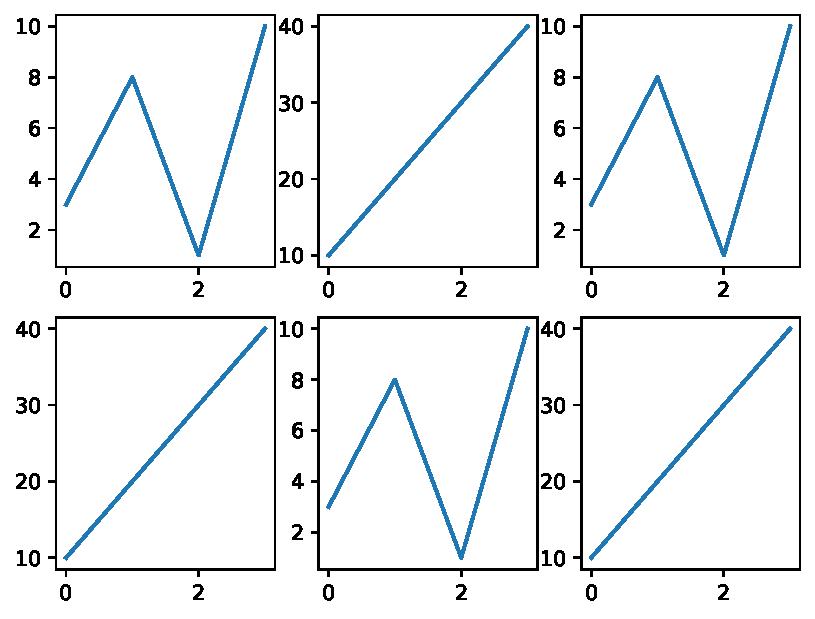
\includegraphics[scale=0.6]{img/grafica1033.pdf}
\end{figure}
\end{code}

\section{Título}

Puede agregar un título a cada gráfico con la función \texttt{title()}.

\begin{code} 2 parcelas, con títulos.

\begin{Shaded}
\begin{Highlighting}[]
\ImportTok{import}\NormalTok{ matplotlib.pyplot }\ImportTok{as}\NormalTok{ plt}
\ImportTok{import}\NormalTok{ numpy }\ImportTok{as}\NormalTok{ np}

\CommentTok{\#plot 1:}
\NormalTok{x }\OperatorTok{=}\NormalTok{ np.array([}\DecValTok{0}\NormalTok{, }\DecValTok{1}\NormalTok{, }\DecValTok{2}\NormalTok{, }\DecValTok{3}\NormalTok{])}
\NormalTok{y }\OperatorTok{=}\NormalTok{ np.array([}\DecValTok{3}\NormalTok{, }\DecValTok{8}\NormalTok{, }\DecValTok{1}\NormalTok{, }\DecValTok{10}\NormalTok{])}

\NormalTok{plt.subplot(}\DecValTok{1}\NormalTok{, }\DecValTok{2}\NormalTok{, }\DecValTok{1}\NormalTok{)}
\NormalTok{plt.plot(x,y)}
\NormalTok{plt.title(}\StringTok{"SALES"}\NormalTok{)}

\CommentTok{\#plot 2:}
\NormalTok{x }\OperatorTok{=}\NormalTok{ np.array([}\DecValTok{0}\NormalTok{, }\DecValTok{1}\NormalTok{, }\DecValTok{2}\NormalTok{, }\DecValTok{3}\NormalTok{])}
\NormalTok{y }\OperatorTok{=}\NormalTok{ np.array([}\DecValTok{10}\NormalTok{, }\DecValTok{20}\NormalTok{, }\DecValTok{30}\NormalTok{, }\DecValTok{40}\NormalTok{])}

\NormalTok{plt.subplot(}\DecValTok{1}\NormalTok{, }\DecValTok{2}\NormalTok{, }\DecValTok{2}\NormalTok{)}
\NormalTok{plt.plot(x,y)}
\NormalTok{plt.title(}\StringTok{"INCOME"}\NormalTok{)}

\NormalTok{plt.show()}
\end{Highlighting}
\end{Shaded}

\begin{figure}
  \centering
  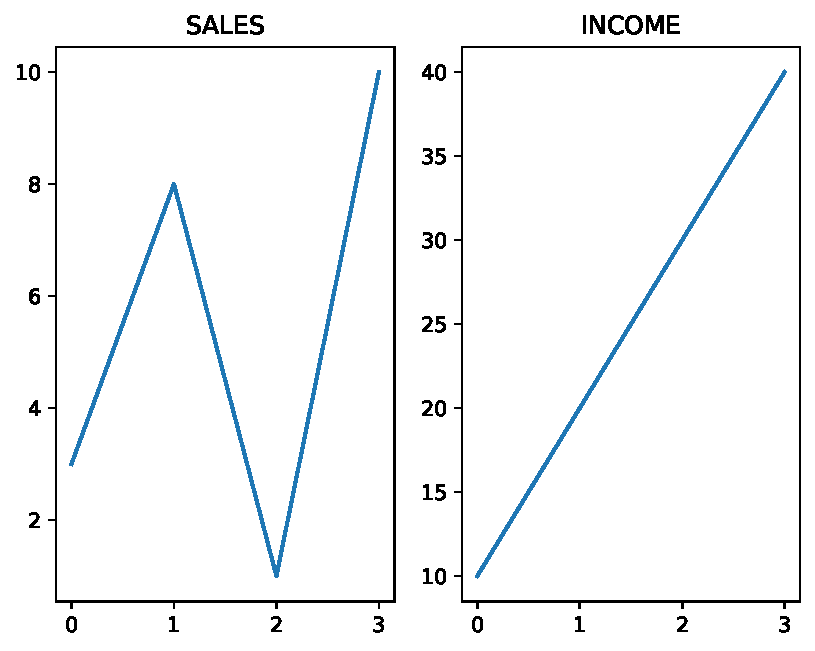
\includegraphics[scale=0.6]{img/grafica1034.pdf}
\end{figure}
\end{code}

\section{Súper título}

Puede agregar un título a toda la figura con la función
\texttt{suptitle()}.

\begin{code} Añade un título para toda la figura.

\begin{Shaded}
\begin{Highlighting}[]
\ImportTok{import}\NormalTok{ matplotlib.pyplot }\ImportTok{as}\NormalTok{ plt}
\ImportTok{import}\NormalTok{ numpy }\ImportTok{as}\NormalTok{ np}

\CommentTok{\#plot 1:}
\NormalTok{x }\OperatorTok{=}\NormalTok{ np.array([}\DecValTok{0}\NormalTok{, }\DecValTok{1}\NormalTok{, }\DecValTok{2}\NormalTok{, }\DecValTok{3}\NormalTok{])}
\NormalTok{y }\OperatorTok{=}\NormalTok{ np.array([}\DecValTok{3}\NormalTok{, }\DecValTok{8}\NormalTok{, }\DecValTok{1}\NormalTok{, }\DecValTok{10}\NormalTok{])}

\NormalTok{plt.subplot(}\DecValTok{1}\NormalTok{, }\DecValTok{2}\NormalTok{, }\DecValTok{1}\NormalTok{)}
\NormalTok{plt.plot(x,y)}
\NormalTok{plt.title(}\StringTok{"SALES"}\NormalTok{)}

\CommentTok{\#plot 2:}
\NormalTok{x }\OperatorTok{=}\NormalTok{ np.array([}\DecValTok{0}\NormalTok{, }\DecValTok{1}\NormalTok{, }\DecValTok{2}\NormalTok{, }\DecValTok{3}\NormalTok{])}
\NormalTok{y }\OperatorTok{=}\NormalTok{ np.array([}\DecValTok{10}\NormalTok{, }\DecValTok{20}\NormalTok{, }\DecValTok{30}\NormalTok{, }\DecValTok{40}\NormalTok{])}

\NormalTok{plt.subplot(}\DecValTok{1}\NormalTok{, }\DecValTok{2}\NormalTok{, }\DecValTok{2}\NormalTok{)}
\NormalTok{plt.plot(x,y)}
\NormalTok{plt.title(}\StringTok{"INCOME"}\NormalTok{)}

\NormalTok{plt.suptitle(}\StringTok{"MY SHOP"}\NormalTok{)}
\NormalTok{plt.show()}
\end{Highlighting}
\end{Shaded}

\begin{figure}
  \centering
  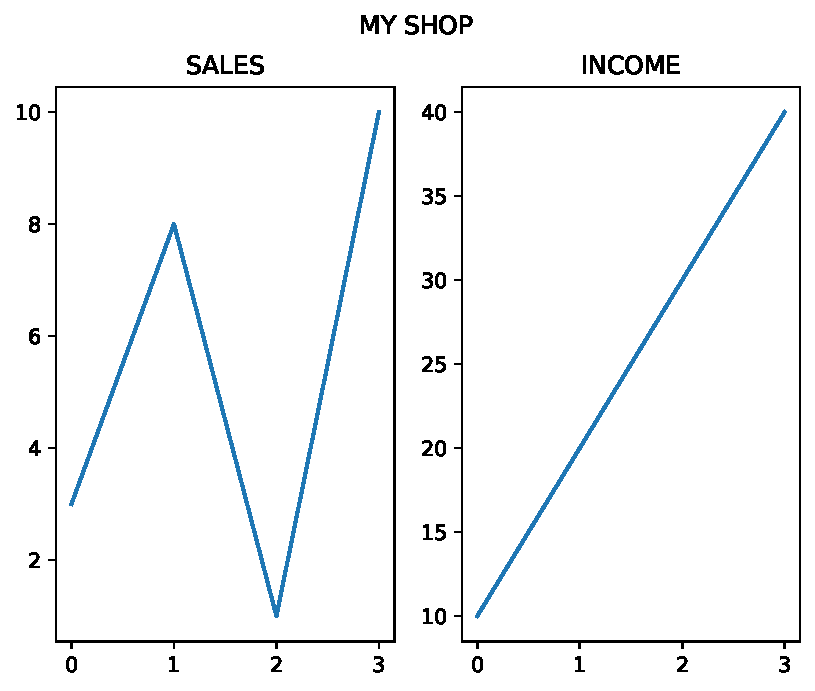
\includegraphics[scale=0.6]{img/grafica1035.pdf}
\end{figure}
\end{code}

\section{Gráficos de dispersión}

Con \texttt{Pyplot}, puede utilizar la función \texttt{scatter()} para
dibujar un diagrama de dispersión.

La función \texttt{scatter()} traza un punto para cada observación.
Necesita dos matrices de la misma longitud, una para los valores del eje
\(x\) y otra para los valores del eje \(y\).

\begin{code} Un diagrama de dispersión simple.

\begin{Shaded}
\begin{Highlighting}[]
\ImportTok{import}\NormalTok{ matplotlib.pyplot }\ImportTok{as}\NormalTok{ plt}
\ImportTok{import}\NormalTok{ numpy }\ImportTok{as}\NormalTok{ np}

\NormalTok{x }\OperatorTok{=}\NormalTok{ np.array([}\DecValTok{5}\NormalTok{,}\DecValTok{7}\NormalTok{,}\DecValTok{8}\NormalTok{,}\DecValTok{7}\NormalTok{,}\DecValTok{2}\NormalTok{,}\DecValTok{17}\NormalTok{,}\DecValTok{2}\NormalTok{,}\DecValTok{9}\NormalTok{,}\DecValTok{4}\NormalTok{,}\DecValTok{11}\NormalTok{,}\DecValTok{12}\NormalTok{,}\DecValTok{9}\NormalTok{,}\DecValTok{6}\NormalTok{])}
\NormalTok{y }\OperatorTok{=}\NormalTok{ np.array([}\DecValTok{99}\NormalTok{,}\DecValTok{86}\NormalTok{,}\DecValTok{87}\NormalTok{,}\DecValTok{88}\NormalTok{,}\DecValTok{111}\NormalTok{,}\DecValTok{86}\NormalTok{,}\DecValTok{103}\NormalTok{,}\DecValTok{87}\NormalTok{,}\DecValTok{94}\NormalTok{,}\DecValTok{78}\NormalTok{,}\DecValTok{77}\NormalTok{,}\DecValTok{85}\NormalTok{,}\DecValTok{86}\NormalTok{])}

\NormalTok{plt.scatter(x, y)}
\NormalTok{plt.show()}
\end{Highlighting}
\end{Shaded}

\begin{figure}
  \centering
  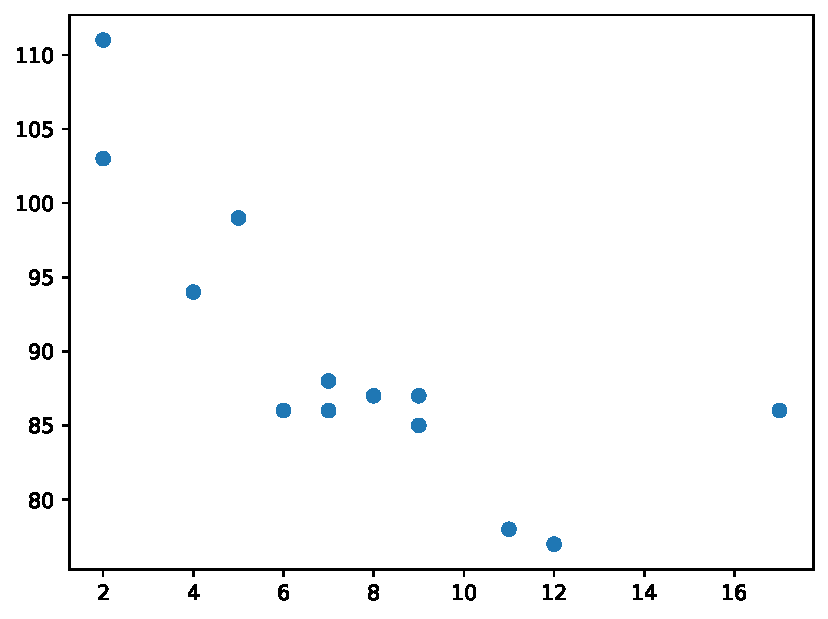
\includegraphics[scale=0.6]{img/grafica1036.pdf}
\end{figure}
\end{code}

La observación en el ejemplo anterior es el resultado de 13 automóviles.

El eje \(x\) muestra la antigüedad del coche y el eje \(y\) muestra la
velocidad del automóvil cuando pasa.

¿Existe alguna relación entre las observaciones?. Parece que cuanto más
nuevo es el coche, más rápido va, pero eso podría ser una coincidencia,
después de todo sólo registramos 13 coches.

\section{Comparar gráficos}

En el ejemplo anterior, parece haber una relación entre la velocidad y
la edad, pero ¿qué pasa si graficamos también las observaciones de otro
día? ¿El diagrama de dispersión nos dirá algo más?

\begin{code} Dibuje dos gráficos en la misma figura.

\begin{Shaded}
\begin{Highlighting}[]
\ImportTok{import}\NormalTok{ matplotlib.pyplot }\ImportTok{as}\NormalTok{ plt}
\ImportTok{import}\NormalTok{ numpy }\ImportTok{as}\NormalTok{ np}

\CommentTok{\#day one, the age and speed of 13 cars:}
\NormalTok{x }\OperatorTok{=}\NormalTok{ np.array([}\DecValTok{5}\NormalTok{,}\DecValTok{7}\NormalTok{,}\DecValTok{8}\NormalTok{,}\DecValTok{7}\NormalTok{,}\DecValTok{2}\NormalTok{,}\DecValTok{17}\NormalTok{,}\DecValTok{2}\NormalTok{,}\DecValTok{9}\NormalTok{,}\DecValTok{4}\NormalTok{,}\DecValTok{11}\NormalTok{,}\DecValTok{12}\NormalTok{,}\DecValTok{9}\NormalTok{,}\DecValTok{6}\NormalTok{])}
\NormalTok{y }\OperatorTok{=}\NormalTok{ np.array([}\DecValTok{99}\NormalTok{,}\DecValTok{86}\NormalTok{,}\DecValTok{87}\NormalTok{,}\DecValTok{88}\NormalTok{,}\DecValTok{111}\NormalTok{,}\DecValTok{86}\NormalTok{,}\DecValTok{103}\NormalTok{,}\DecValTok{87}\NormalTok{,}\DecValTok{94}\NormalTok{,}\DecValTok{78}\NormalTok{,}\DecValTok{77}\NormalTok{,}\DecValTok{85}\NormalTok{,}\DecValTok{86}\NormalTok{])}
\NormalTok{plt.scatter(x, y)}

\CommentTok{\#day two, the age and speed of 15 cars:}
\NormalTok{x }\OperatorTok{=}\NormalTok{ np.array([}\DecValTok{2}\NormalTok{,}\DecValTok{2}\NormalTok{,}\DecValTok{8}\NormalTok{,}\DecValTok{1}\NormalTok{,}\DecValTok{15}\NormalTok{,}\DecValTok{8}\NormalTok{,}\DecValTok{12}\NormalTok{,}\DecValTok{9}\NormalTok{,}\DecValTok{7}\NormalTok{,}\DecValTok{3}\NormalTok{,}\DecValTok{11}\NormalTok{,}\DecValTok{4}\NormalTok{,}\DecValTok{7}\NormalTok{,}\DecValTok{14}\NormalTok{,}\DecValTok{12}\NormalTok{])}
\NormalTok{y }\OperatorTok{=}\NormalTok{ np.array([}\DecValTok{100}\NormalTok{,}\DecValTok{105}\NormalTok{,}\DecValTok{84}\NormalTok{,}\DecValTok{105}\NormalTok{,}\DecValTok{90}\NormalTok{,}\DecValTok{99}\NormalTok{,}\DecValTok{90}\NormalTok{,}\DecValTok{95}\NormalTok{,}\DecValTok{94}\NormalTok{,}\DecValTok{100}\NormalTok{,}\DecValTok{79}\NormalTok{,}\DecValTok{112}\NormalTok{,}\DecValTok{91}\NormalTok{,}\DecValTok{80}\NormalTok{,}\DecValTok{85}\NormalTok{])}
\NormalTok{plt.scatter(x, y)}

\NormalTok{plt.show()}
\end{Highlighting}
\end{Shaded}

\begin{figure}
  \centering
  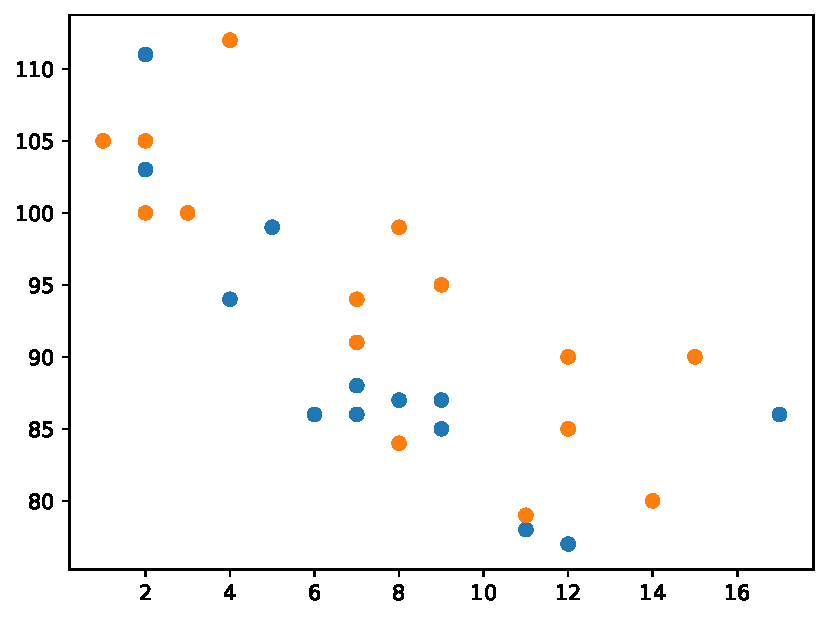
\includegraphics[scale=0.6]{img/grafica1037.pdf}
\end{figure}
\end{code}

\textbf{Nota}: Los dos gráficos están representados con dos colores
diferentes, por defecto azul y naranja.

Comparando ambos gráficos, creo que es seguro decir que ambos nos llevan
a la misma conclusión: cuanto más nuevo es el coche, más rápido va.

\section{Colores}

Puede establecer su propio color para cada gráfico de dispersión con
\texttt{color} o el argumento \texttt{c}.

\begin{code} Establezca su propio color de marcadores.

\begin{Shaded}
\begin{Highlighting}[]
\ImportTok{import}\NormalTok{ matplotlib.pyplot }\ImportTok{as}\NormalTok{ plt}
\ImportTok{import}\NormalTok{ numpy }\ImportTok{as}\NormalTok{ np}

\NormalTok{x }\OperatorTok{=}\NormalTok{ np.array([}\DecValTok{5}\NormalTok{,}\DecValTok{7}\NormalTok{,}\DecValTok{8}\NormalTok{,}\DecValTok{7}\NormalTok{,}\DecValTok{2}\NormalTok{,}\DecValTok{17}\NormalTok{,}\DecValTok{2}\NormalTok{,}\DecValTok{9}\NormalTok{,}\DecValTok{4}\NormalTok{,}\DecValTok{11}\NormalTok{,}\DecValTok{12}\NormalTok{,}\DecValTok{9}\NormalTok{,}\DecValTok{6}\NormalTok{])}
\NormalTok{y }\OperatorTok{=}\NormalTok{ np.array([}\DecValTok{99}\NormalTok{,}\DecValTok{86}\NormalTok{,}\DecValTok{87}\NormalTok{,}\DecValTok{88}\NormalTok{,}\DecValTok{111}\NormalTok{,}\DecValTok{86}\NormalTok{,}\DecValTok{103}\NormalTok{,}\DecValTok{87}\NormalTok{,}\DecValTok{94}\NormalTok{,}\DecValTok{78}\NormalTok{,}\DecValTok{77}\NormalTok{,}\DecValTok{85}\NormalTok{,}\DecValTok{86}\NormalTok{])}
\NormalTok{plt.scatter(x, y, color }\OperatorTok{=} \StringTok{\textquotesingle{}hotpink\textquotesingle{}}\NormalTok{)}

\NormalTok{x }\OperatorTok{=}\NormalTok{ np.array([}\DecValTok{2}\NormalTok{,}\DecValTok{2}\NormalTok{,}\DecValTok{8}\NormalTok{,}\DecValTok{1}\NormalTok{,}\DecValTok{15}\NormalTok{,}\DecValTok{8}\NormalTok{,}\DecValTok{12}\NormalTok{,}\DecValTok{9}\NormalTok{,}\DecValTok{7}\NormalTok{,}\DecValTok{3}\NormalTok{,}\DecValTok{11}\NormalTok{,}\DecValTok{4}\NormalTok{,}\DecValTok{7}\NormalTok{,}\DecValTok{14}\NormalTok{,}\DecValTok{12}\NormalTok{])}
\NormalTok{y }\OperatorTok{=}\NormalTok{ np.array([}\DecValTok{100}\NormalTok{,}\DecValTok{105}\NormalTok{,}\DecValTok{84}\NormalTok{,}\DecValTok{105}\NormalTok{,}\DecValTok{90}\NormalTok{,}\DecValTok{99}\NormalTok{,}\DecValTok{90}\NormalTok{,}\DecValTok{95}\NormalTok{,}\DecValTok{94}\NormalTok{,}\DecValTok{100}\NormalTok{,}\DecValTok{79}\NormalTok{,}\DecValTok{112}\NormalTok{,}\DecValTok{91}\NormalTok{,}\DecValTok{80}\NormalTok{,}\DecValTok{85}\NormalTok{])}
\NormalTok{plt.scatter(x, y, color }\OperatorTok{=} \StringTok{\textquotesingle{}\#88c999\textquotesingle{}}\NormalTok{)}

\NormalTok{plt.show()}
\end{Highlighting}
\end{Shaded}

\begin{figure}
  \centering
  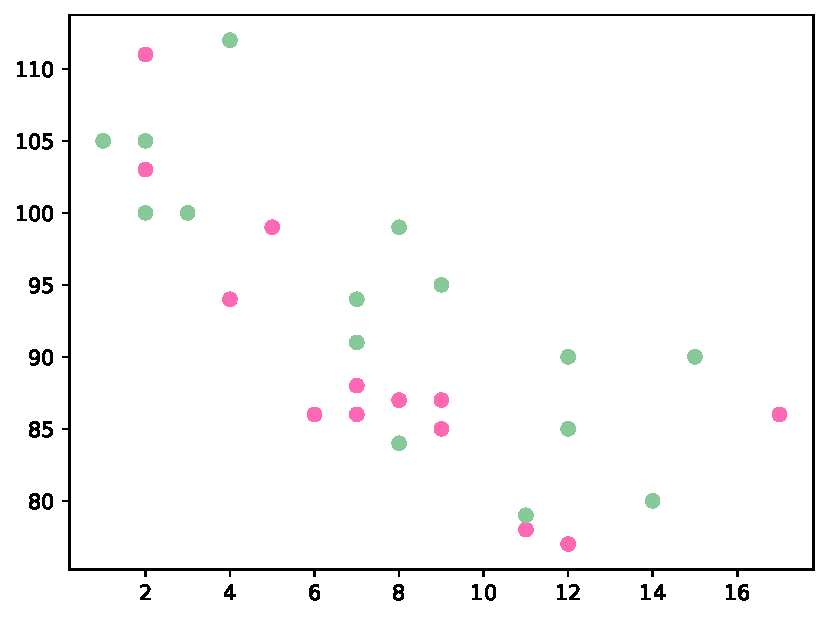
\includegraphics[scale=0.6]{img/grafica1038.pdf}
\end{figure}
\end{code}

\section{Colorear cada punto}

Es posible establecer un color específico para cada punto utilizando una
matriz de colores como valor para el cargumento.

\textbf{Nota}: No puede usar el argumento \texttt{color} para esto, solo
el argumento \texttt{c}.\\

\begin{code} Colorear puntos de dispersión.
\begin{Shaded}
\begin{Highlighting}[]
\ImportTok{import}\NormalTok{ matplotlib.pyplot }\ImportTok{as}\NormalTok{ plt}
\ImportTok{import}\NormalTok{ numpy }\ImportTok{as}\NormalTok{ np}

\NormalTok{x }\OperatorTok{=}\NormalTok{ np.array([}\DecValTok{5}\NormalTok{,}\DecValTok{7}\NormalTok{,}\DecValTok{8}\NormalTok{,}\DecValTok{7}\NormalTok{,}\DecValTok{2}\NormalTok{,}\DecValTok{17}\NormalTok{,}\DecValTok{2}\NormalTok{,}\DecValTok{9}\NormalTok{,}\DecValTok{4}\NormalTok{,}\DecValTok{11}\NormalTok{,}\DecValTok{12}\NormalTok{,}\DecValTok{9}\NormalTok{,}\DecValTok{6}\NormalTok{])}
\NormalTok{y }\OperatorTok{=}\NormalTok{ np.array([}\DecValTok{99}\NormalTok{,}\DecValTok{86}\NormalTok{,}\DecValTok{87}\NormalTok{,}\DecValTok{88}\NormalTok{,}\DecValTok{111}\NormalTok{,}\DecValTok{86}\NormalTok{,}\DecValTok{103}\NormalTok{,}\DecValTok{87}\NormalTok{,}\DecValTok{94}\NormalTok{,}\DecValTok{78}\NormalTok{,}\DecValTok{77}\NormalTok{,}\DecValTok{85}\NormalTok{,}\DecValTok{86}\NormalTok{])}
\NormalTok{colors }\OperatorTok{=}\NormalTok{ np.array([}\StringTok{"red"}\NormalTok{,}\StringTok{"green"}\NormalTok{,}\StringTok{"blue"}\NormalTok{,}\StringTok{"yellow"}\NormalTok{,}\StringTok{"pink"}\NormalTok{,}\StringTok{"black"}\NormalTok{,}\StringTok{"orange"}\NormalTok{,}\StringTok{"purple"}\NormalTok{,}
    \StringTok{"beige"}\NormalTok{,}\StringTok{"brown"}\NormalTok{,}\StringTok{"gray"}\NormalTok{,}\StringTok{"cyan"}\NormalTok{,}\StringTok{"magenta"}\NormalTok{])}

\NormalTok{plt.scatter(x, y, c}\OperatorTok{=}\NormalTok{colors)}

\NormalTok{plt.show()}
\end{Highlighting}
\end{Shaded}

\begin{figure}
  \centering
  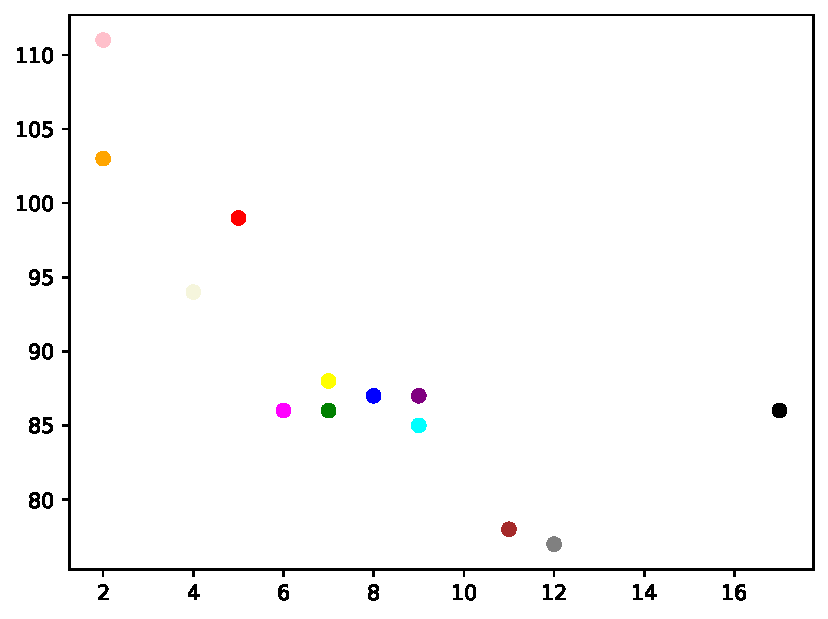
\includegraphics[scale=0.6]{img/grafica1039.pdf}
\end{figure}
\end{code}

\section{Mapa de colores}

El módulo \texttt{Matplotlib} tiene varios mapas de colores disponibles.

Un mapa de colores es una lista de colores, donde cada color tiene un
valor que varía de 0 a 100.

A continuación se muestra un ejemplo de un mapa de colores:
\begin{figure}
  \centering
  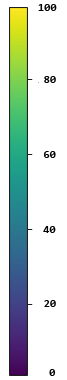
\includegraphics[scale=0.6]{img/img_colorbar.png}
\end{figure}


Este mapa de colores se llama
\emph{\textquotesingle viridis\textquotesingle{}} y como puedes ver,
varía desde 0, que es un color púrpura, hasta 100, que es un color
amarillo.

\subsubsection{Cómo utilizar el mapa de colores}

Puede especificar el mapa de colores con el argumento de palabra clave
\texttt{cmap}, en este caso
\emph{\textquotesingle viridis\textquotesingle{}} que es uno de los
mapas de colores integrados disponibles en \texttt{Matplotlib}.

Además, debes crear una matriz con valores (de 0 a 100), un valor para
cada punto en el diagrama de dispersión.\\

\begin{code} Cree una matriz de colores y especifique un mapa de
colores en el gráfico de dispersión.

\begin{Shaded}
\begin{Highlighting}[]
\ImportTok{import}\NormalTok{ matplotlib.pyplot }\ImportTok{as}\NormalTok{ plt}
\ImportTok{import}\NormalTok{ numpy }\ImportTok{as}\NormalTok{ np}

\NormalTok{x }\OperatorTok{=}\NormalTok{ np.array([}\DecValTok{5}\NormalTok{,}\DecValTok{7}\NormalTok{,}\DecValTok{8}\NormalTok{,}\DecValTok{7}\NormalTok{,}\DecValTok{2}\NormalTok{,}\DecValTok{17}\NormalTok{,}\DecValTok{2}\NormalTok{,}\DecValTok{9}\NormalTok{,}\DecValTok{4}\NormalTok{,}\DecValTok{11}\NormalTok{,}\DecValTok{12}\NormalTok{,}\DecValTok{9}\NormalTok{,}\DecValTok{6}\NormalTok{])}
\NormalTok{y }\OperatorTok{=}\NormalTok{ np.array([}\DecValTok{99}\NormalTok{,}\DecValTok{86}\NormalTok{,}\DecValTok{87}\NormalTok{,}\DecValTok{88}\NormalTok{,}\DecValTok{111}\NormalTok{,}\DecValTok{86}\NormalTok{,}\DecValTok{103}\NormalTok{,}\DecValTok{87}\NormalTok{,}\DecValTok{94}\NormalTok{,}\DecValTok{78}\NormalTok{,}\DecValTok{77}\NormalTok{,}\DecValTok{85}\NormalTok{,}\DecValTok{86}\NormalTok{])}
\NormalTok{colors }\OperatorTok{=}\NormalTok{ np.array([}\DecValTok{0}\NormalTok{, }\DecValTok{10}\NormalTok{, }\DecValTok{20}\NormalTok{, }\DecValTok{30}\NormalTok{, }\DecValTok{40}\NormalTok{, }\DecValTok{45}\NormalTok{, }\DecValTok{50}\NormalTok{, }\DecValTok{55}\NormalTok{, }\DecValTok{60}\NormalTok{, }\DecValTok{70}\NormalTok{, }\DecValTok{80}\NormalTok{, }\DecValTok{90}\NormalTok{, }\DecValTok{100}\NormalTok{])}

\NormalTok{plt.scatter(x, y, c}\OperatorTok{=}\NormalTok{colors, cmap}\OperatorTok{=}\StringTok{\textquotesingle{}viridis\textquotesingle{}}\NormalTok{)}

\NormalTok{plt.show()}
\end{Highlighting}
\end{Shaded}

\begin{figure}
  \centering
  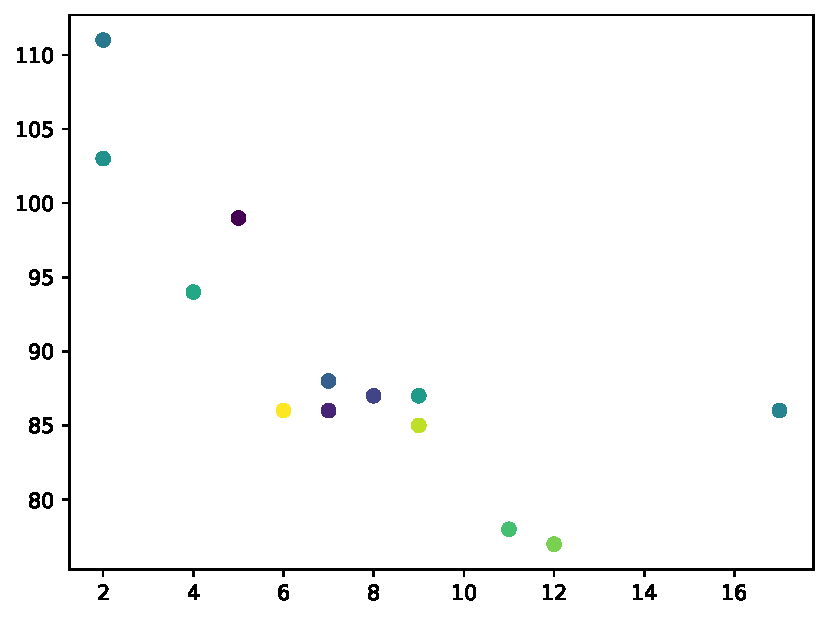
\includegraphics[scale=0.6]{img/grafica1040.pdf}
\end{figure}
\end{code}

Puede incluir el mapa de colores en el dibujo incluyendo la declaración \texttt{plt.colorbar()}.\\

\begin{code} Incluya el mapa de colores real.

\begin{Shaded}
\begin{Highlighting}[]
\ImportTok{import}\NormalTok{ matplotlib.pyplot }\ImportTok{as}\NormalTok{ plt}
\ImportTok{import}\NormalTok{ numpy }\ImportTok{as}\NormalTok{ np}

\NormalTok{x }\OperatorTok{=}\NormalTok{ np.array([}\DecValTok{5}\NormalTok{,}\DecValTok{7}\NormalTok{,}\DecValTok{8}\NormalTok{,}\DecValTok{7}\NormalTok{,}\DecValTok{2}\NormalTok{,}\DecValTok{17}\NormalTok{,}\DecValTok{2}\NormalTok{,}\DecValTok{9}\NormalTok{,}\DecValTok{4}\NormalTok{,}\DecValTok{11}\NormalTok{,}\DecValTok{12}\NormalTok{,}\DecValTok{9}\NormalTok{,}\DecValTok{6}\NormalTok{])}
\NormalTok{y }\OperatorTok{=}\NormalTok{ np.array([}\DecValTok{99}\NormalTok{,}\DecValTok{86}\NormalTok{,}\DecValTok{87}\NormalTok{,}\DecValTok{88}\NormalTok{,}\DecValTok{111}\NormalTok{,}\DecValTok{86}\NormalTok{,}\DecValTok{103}\NormalTok{,}\DecValTok{87}\NormalTok{,}\DecValTok{94}\NormalTok{,}\DecValTok{78}\NormalTok{,}\DecValTok{77}\NormalTok{,}\DecValTok{85}\NormalTok{,}\DecValTok{86}\NormalTok{])}
\NormalTok{colors }\OperatorTok{=}\NormalTok{ np.array([}\DecValTok{0}\NormalTok{, }\DecValTok{10}\NormalTok{, }\DecValTok{20}\NormalTok{, }\DecValTok{30}\NormalTok{, }\DecValTok{40}\NormalTok{, }\DecValTok{45}\NormalTok{, }\DecValTok{50}\NormalTok{, }\DecValTok{55}\NormalTok{, }\DecValTok{60}\NormalTok{, }\DecValTok{70}\NormalTok{, }\DecValTok{80}\NormalTok{, }\DecValTok{90}\NormalTok{, }\DecValTok{100}\NormalTok{])}

\NormalTok{plt.scatter(x, y, c}\OperatorTok{=}\NormalTok{colors, cmap}\OperatorTok{=}\StringTok{\textquotesingle{}gist\_rainbow\textquotesingle{}}\NormalTok{)}

\NormalTok{plt.colorbar()}

\NormalTok{plt.show()}
\end{Highlighting}
\end{Shaded}

\begin{figure}
  \centering
  \includegraphics[scale=0.6]{img/grafica1041.pdf}
\end{figure}
\end{code}

\section{Mapas de colores disponibles}

Puede elegir cualquiera de los
\href{https://matplotlib.org/stable/users/explain/colors/colormaps.html}{mapas
de colores incorporados}.

\begin{Shaded}
\begin{Highlighting}[]
\ImportTok{from}\NormalTok{ matplotlib }\ImportTok{import}\NormalTok{ colormaps}
\BuiltInTok{list}\NormalTok{(colormaps)}
\end{Highlighting}
\end{Shaded}

\begin{verbatim}
['magma',
 'inferno',
 'plasma',
 'viridis',
 'cividis',
 'twilight',
 'twilight_shifted',
 'turbo',
 'Blues',
 'BrBG',
 'BuGn',
 'BuPu',
 'CMRmap',
 'GnBu',
 'Greens',
 'Greys',
 'OrRd',
 'Oranges',
 'PRGn',
 'PiYG',
 'PuBu',
 'PuBuGn',
 'PuOr',
 'PuRd',
 'Purples',
 'RdBu',
 'RdGy',
 'RdPu',
 'RdYlBu',
 'RdYlGn',
 'Reds',
 'Spectral',
 'Wistia',
 'YlGn',
 'YlGnBu',
 'YlOrBr',
 'YlOrRd',
 'afmhot',
 'autumn',
 'binary',
 'bone',
 'brg',
 'bwr',
 'cool',
 'coolwarm',
 'copper',
 'cubehelix',
 'flag',
 'gist_earth',
 'gist_gray',
 'gist_heat',
 'gist_ncar',
 'gist_rainbow',
 'gist_stern',
 'gist_yarg',
 'gnuplot',
 'gnuplot2',
 'gray',
 'hot',
 'hsv',
 'jet',
 'nipy_spectral',
 'ocean',
 'pink',
 'prism',
 'rainbow',
 'seismic',
 'spring',
 'summer',
 'terrain',
 'winter',
 'Accent',
 'Dark2',
 'Paired',
 'Pastel1',
 'Pastel2',
 'Set1',
 'Set2',
 'Set3',
 'tab10',
 'tab20',
 'tab20b',
 'tab20c',
 'grey',
 'gist_grey',
 'gist_yerg',
 'Grays',
 'magma_r',
 'inferno_r',
 'plasma_r',
 'viridis_r',
 'cividis_r',
 'twilight_r',
 'twilight_shifted_r',
 'turbo_r',
 'Blues_r',
 'BrBG_r',
 'BuGn_r',
 'BuPu_r',
 'CMRmap_r',
 'GnBu_r',
 'Greens_r',
 'Greys_r',
 'OrRd_r',
 'Oranges_r',
 'PRGn_r',
 'PiYG_r',
 'PuBu_r',
 'PuBuGn_r',
 'PuOr_r',
 'PuRd_r',
 'Purples_r',
 'RdBu_r',
 'RdGy_r',
 'RdPu_r',
 'RdYlBu_r',
 'RdYlGn_r',
 'Reds_r',
 'Spectral_r',
 'Wistia_r',
 'YlGn_r',
 'YlGnBu_r',
 'YlOrBr_r',
 'YlOrRd_r',
 'afmhot_r',
 'autumn_r',
 'binary_r',
 'bone_r',
 'brg_r',
 'bwr_r',
 'cool_r',
 'coolwarm_r',
 'copper_r',
 'cubehelix_r',
 'flag_r',
 'gist_earth_r',
 'gist_gray_r',
 'gist_heat_r',
 'gist_ncar_r',
 'gist_rainbow_r',
 'gist_stern_r',
 'gist_yarg_r',
 'gnuplot_r',
 'gnuplot2_r',
 'gray_r',
 'hot_r',
 'hsv_r',
 'jet_r',
 'nipy_spectral_r',
 'ocean_r',
 'pink_r',
 'prism_r',
 'rainbow_r',
 'seismic_r',
 'spring_r',
 'summer_r',
 'terrain_r',
 'winter_r',
 'Accent_r',
 'Dark2_r',
 'Paired_r',
 'Pastel1_r',
 'Pastel2_r',
 'Set1_r',
 'Set2_r',
 'Set3_r',
 'tab10_r',
 'tab20_r',
 'tab20b_r',
 'tab20c_r']
\end{verbatim}

\section{Tamaño}

Puede cambiar el tamaño de los puntos con el sargumento.

Al igual que con los colores, asegúrese de que la matriz de tamaños
tenga la misma longitud que las matrices de ejes \(x\) y \(y\).

\begin{code} Establezca su propio tamaño para los marcadores.

\begin{Shaded}
\begin{Highlighting}[]
\ImportTok{import}\NormalTok{ matplotlib.pyplot }\ImportTok{as}\NormalTok{ plt}
\ImportTok{import}\NormalTok{ numpy }\ImportTok{as}\NormalTok{ np}

\NormalTok{x }\OperatorTok{=}\NormalTok{ np.array([}\DecValTok{5}\NormalTok{,}\DecValTok{7}\NormalTok{,}\DecValTok{8}\NormalTok{,}\DecValTok{7}\NormalTok{,}\DecValTok{2}\NormalTok{,}\DecValTok{17}\NormalTok{,}\DecValTok{2}\NormalTok{,}\DecValTok{9}\NormalTok{,}\DecValTok{4}\NormalTok{,}\DecValTok{11}\NormalTok{,}\DecValTok{12}\NormalTok{,}\DecValTok{9}\NormalTok{,}\DecValTok{6}\NormalTok{])}
\NormalTok{y }\OperatorTok{=}\NormalTok{ np.array([}\DecValTok{99}\NormalTok{,}\DecValTok{86}\NormalTok{,}\DecValTok{87}\NormalTok{,}\DecValTok{88}\NormalTok{,}\DecValTok{111}\NormalTok{,}\DecValTok{86}\NormalTok{,}\DecValTok{103}\NormalTok{,}\DecValTok{87}\NormalTok{,}\DecValTok{94}\NormalTok{,}\DecValTok{78}\NormalTok{,}\DecValTok{77}\NormalTok{,}\DecValTok{85}\NormalTok{,}\DecValTok{86}\NormalTok{])}
\NormalTok{sizes }\OperatorTok{=}\NormalTok{ np.array([}\DecValTok{20}\NormalTok{,}\DecValTok{50}\NormalTok{,}\DecValTok{100}\NormalTok{,}\DecValTok{200}\NormalTok{,}\DecValTok{500}\NormalTok{,}\DecValTok{1000}\NormalTok{,}\DecValTok{60}\NormalTok{,}\DecValTok{90}\NormalTok{,}\DecValTok{10}\NormalTok{,}\DecValTok{300}\NormalTok{,}\DecValTok{600}\NormalTok{,}\DecValTok{800}\NormalTok{,}\DecValTok{75}\NormalTok{])}

\NormalTok{plt.scatter(x, y, s}\OperatorTok{=}\NormalTok{sizes)}
\NormalTok{plt.show()}
\end{Highlighting}
\end{Shaded}

\begin{figure}
  \centering
  \includegraphics[scale=0.6]{img/grafica1042.pdf}
\end{figure}
\end{code}

\section{Transparencia}

Puede ajustar la transparencia de los puntos con el argumento \texttt{alpha}.

Al igual que con los colores, es posbile ajustar la transparencia a los
puntos individualmente, sólo asegúrese de que la matriz de tamaños tenga
la misma longitud que las matrices de ejes \(x\) y \(y\).\\

\begin{code} Establezca su propio tamaño para los marcadores.

\begin{Shaded}
\begin{Highlighting}[]
\ImportTok{import}\NormalTok{ matplotlib.pyplot }\ImportTok{as}\NormalTok{ plt}
\ImportTok{import}\NormalTok{ numpy }\ImportTok{as}\NormalTok{ np}

\NormalTok{x }\OperatorTok{=}\NormalTok{ np.array([}\DecValTok{5}\NormalTok{,}\DecValTok{7}\NormalTok{,}\DecValTok{8}\NormalTok{,}\DecValTok{7}\NormalTok{,}\DecValTok{2}\NormalTok{,}\DecValTok{17}\NormalTok{,}\DecValTok{2}\NormalTok{,}\DecValTok{9}\NormalTok{,}\DecValTok{4}\NormalTok{,}\DecValTok{11}\NormalTok{,}\DecValTok{12}\NormalTok{,}\DecValTok{9}\NormalTok{,}\DecValTok{6}\NormalTok{])}
\NormalTok{y }\OperatorTok{=}\NormalTok{ np.array([}\DecValTok{99}\NormalTok{,}\DecValTok{86}\NormalTok{,}\DecValTok{87}\NormalTok{,}\DecValTok{88}\NormalTok{,}\DecValTok{111}\NormalTok{,}\DecValTok{86}\NormalTok{,}\DecValTok{103}\NormalTok{,}\DecValTok{87}\NormalTok{,}\DecValTok{94}\NormalTok{,}\DecValTok{78}\NormalTok{,}\DecValTok{77}\NormalTok{,}\DecValTok{85}\NormalTok{,}\DecValTok{86}\NormalTok{])}
\NormalTok{sizes }\OperatorTok{=}\NormalTok{ np.array([}\DecValTok{20}\NormalTok{,}\DecValTok{50}\NormalTok{,}\DecValTok{100}\NormalTok{,}\DecValTok{200}\NormalTok{,}\DecValTok{500}\NormalTok{,}\DecValTok{1000}\NormalTok{,}\DecValTok{60}\NormalTok{,}\DecValTok{90}\NormalTok{,}\DecValTok{10}\NormalTok{,}\DecValTok{300}\NormalTok{,}\DecValTok{600}\NormalTok{,}\DecValTok{800}\NormalTok{,}\DecValTok{75}\NormalTok{])}
\NormalTok{transparency }\OperatorTok{=}\NormalTok{ np.array([}\FloatTok{0.1}\NormalTok{, }\FloatTok{0.2}\NormalTok{, }\FloatTok{0.3}\NormalTok{, }\FloatTok{0.4}\NormalTok{, }\FloatTok{0.5}\NormalTok{, }\FloatTok{0.6}\NormalTok{, }\FloatTok{0.7}\NormalTok{, }\FloatTok{0.8}\NormalTok{, }\FloatTok{0.9}\NormalTok{, }\DecValTok{1}\NormalTok{, }\FloatTok{0.9}\NormalTok{, }\FloatTok{0.8}\NormalTok{, }\FloatTok{0.3}\NormalTok{])}

\NormalTok{plt.scatter(x, y, s}\OperatorTok{=}\NormalTok{sizes, alpha}\OperatorTok{=}\NormalTok{transparency)}
\NormalTok{plt.show()}
\end{Highlighting}
\end{Shaded}

\begin{figure}
  \centering
  \includegraphics[scale=0.6]{img/grafica1043.pdf}
\end{figure}
\end{code}

\section{Combinar color, tamaño y alfa}

Se puede combinar un mapa de colores con diferentes tamaños de puntos.
Esto se visualiza mejor si los puntos son transparentes.\\

\begin{code} Crear matrices aleatorias con 100 valores para puntos \(x\), puntos \(y\), colores y tamaños.

\begin{Shaded}
\begin{Highlighting}[]
\ImportTok{import}\NormalTok{ matplotlib.pyplot }\ImportTok{as}\NormalTok{ plt}
\ImportTok{import}\NormalTok{ numpy }\ImportTok{as}\NormalTok{ np}

\NormalTok{x }\OperatorTok{=}\NormalTok{ np.random.randint(}\DecValTok{100}\NormalTok{, size}\OperatorTok{=}\NormalTok{(}\DecValTok{100}\NormalTok{))}
\NormalTok{y }\OperatorTok{=}\NormalTok{ np.random.randint(}\DecValTok{100}\NormalTok{, size}\OperatorTok{=}\NormalTok{(}\DecValTok{100}\NormalTok{))}
\NormalTok{colors }\OperatorTok{=}\NormalTok{ np.random.randint(}\DecValTok{100}\NormalTok{, size}\OperatorTok{=}\NormalTok{(}\DecValTok{100}\NormalTok{))}
\NormalTok{sizes }\OperatorTok{=} \DecValTok{10} \OperatorTok{*}\NormalTok{ np.random.randint(}\DecValTok{100}\NormalTok{, size}\OperatorTok{=}\NormalTok{(}\DecValTok{100}\NormalTok{))}

\NormalTok{plt.scatter(x, y, c}\OperatorTok{=}\NormalTok{colors, s}\OperatorTok{=}\NormalTok{sizes, alpha}\OperatorTok{=}\FloatTok{0.5}\NormalTok{, cmap}\OperatorTok{=}\StringTok{\textquotesingle{}nipy\_spectral\textquotesingle{}}\NormalTok{)}
\NormalTok{plt.colorbar()}
\NormalTok{plt.show()}
\end{Highlighting}
\end{Shaded}

\begin{figure}
  \centering
  \includegraphics[scale=0.6]{img/grafica1044.pdf}
\end{figure}
\end{code}

\section{Diagrama de barras}

Con \texttt{Pyplot}, se puede utilizar la función \texttt{bar()} para dibujar gráficos de barras.\\

\begin{code} Dibuja 4 barras.

\begin{Shaded}
\begin{Highlighting}[]
\ImportTok{import}\NormalTok{ matplotlib.pyplot }\ImportTok{as}\NormalTok{ plt}
\ImportTok{import}\NormalTok{ numpy }\ImportTok{as}\NormalTok{ np}

\NormalTok{x }\OperatorTok{=}\NormalTok{ np.array([}\StringTok{"A"}\NormalTok{, }\StringTok{"B"}\NormalTok{, }\StringTok{"C"}\NormalTok{, }\StringTok{"D"}\NormalTok{])}
\NormalTok{y }\OperatorTok{=}\NormalTok{ np.array([}\DecValTok{3}\NormalTok{, }\DecValTok{8}\NormalTok{, }\DecValTok{1}\NormalTok{, }\DecValTok{10}\NormalTok{])}

\NormalTok{plt.bar(x,y)}
\NormalTok{plt.show()}
\end{Highlighting}
\end{Shaded}

\begin{figure}
  \centering
  \includegraphics[scale=0.6]{img/grafica1045.pdf}
\end{figure}
\end{code}

La función \texttt{bar()} toma argumentos que describen el diseño de las
barras.

Las categorías y sus valores representados por el primer y segundo
argumento como matrices.

\section{Barras horizontales}

Si desea que las barras se muestren horizontalmente en lugar de
verticalmente, utilice la función \texttt{barh()}. \\

\begin{code} Dibuja 4 barras horizontales.

\begin{Shaded}
\begin{Highlighting}[]
\ImportTok{import}\NormalTok{ matplotlib.pyplot }\ImportTok{as}\NormalTok{ plt}
\ImportTok{import}\NormalTok{ numpy }\ImportTok{as}\NormalTok{ np}

\NormalTok{x }\OperatorTok{=}\NormalTok{ np.array([}\StringTok{"A"}\NormalTok{, }\StringTok{"B"}\NormalTok{, }\StringTok{"C"}\NormalTok{, }\StringTok{"D"}\NormalTok{])}
\NormalTok{y }\OperatorTok{=}\NormalTok{ np.array([}\DecValTok{3}\NormalTok{, }\DecValTok{8}\NormalTok{, }\DecValTok{1}\NormalTok{, }\DecValTok{10}\NormalTok{])}

\NormalTok{plt.barh(x, y)}
\NormalTok{plt.show()}
\end{Highlighting}
\end{Shaded}

\begin{figure}
  \centering
  \includegraphics[scale=0.6]{img/grafica1046.pdf}
\end{figure}
\end{code}

\section{Color de la barra}

El argumento \texttt{color} de palabra clave \texttt{bar()} y
\texttt{barh()} se utiliza para establecer el color de las barras.

\begin{code} Dibuja 4 barras rojas.

\begin{Shaded}
\begin{Highlighting}[]
\ImportTok{import}\NormalTok{ matplotlib.pyplot }\ImportTok{as}\NormalTok{ plt}
\ImportTok{import}\NormalTok{ numpy }\ImportTok{as}\NormalTok{ np}

\NormalTok{x }\OperatorTok{=}\NormalTok{ np.array([}\StringTok{"A"}\NormalTok{, }\StringTok{"B"}\NormalTok{, }\StringTok{"C"}\NormalTok{, }\StringTok{"D"}\NormalTok{])}
\NormalTok{y }\OperatorTok{=}\NormalTok{ np.array([}\DecValTok{3}\NormalTok{, }\DecValTok{8}\NormalTok{, }\DecValTok{1}\NormalTok{, }\DecValTok{10}\NormalTok{])}

\NormalTok{plt.bar(x, y, color }\OperatorTok{=} \StringTok{"red"}\NormalTok{)}
\NormalTok{plt.show()}
\end{Highlighting}
\end{Shaded}

\begin{figure}
  \centering
  \includegraphics[scale=0.6]{img/grafica1047.pdf}
\end{figure}
\end{code}

\textbf{Nota}. Puede utilizar cualquiera de los 140 \href{https://www.w3schools.com/colors/colors_names.asp}{nombres de
colores admitidos} o valores de \href{https://www.w3schools.com/colors/colors_hexadecimal.asp}{color hexadecimales}.

\section{Ancho de barra}

El argumento \texttt{width} de palabra clave \texttt{bar()} permite
establecer el ancho de las barras. \\

\begin{code} Dibuja 4 barras muy finas.

\begin{Shaded}
\begin{Highlighting}[]
\ImportTok{import}\NormalTok{ matplotlib.pyplot }\ImportTok{as}\NormalTok{ plt}
\ImportTok{import}\NormalTok{ numpy }\ImportTok{as}\NormalTok{ np}

\NormalTok{x }\OperatorTok{=}\NormalTok{ np.array([}\StringTok{"A"}\NormalTok{, }\StringTok{"B"}\NormalTok{, }\StringTok{"C"}\NormalTok{, }\StringTok{"D"}\NormalTok{])}
\NormalTok{y }\OperatorTok{=}\NormalTok{ np.array([}\DecValTok{3}\NormalTok{, }\DecValTok{8}\NormalTok{, }\DecValTok{1}\NormalTok{, }\DecValTok{10}\NormalTok{])}
\NormalTok{width }\OperatorTok{=}\NormalTok{ np.array([}\FloatTok{0.1}\NormalTok{, }\DecValTok{1}\NormalTok{, }\FloatTok{0.5}\NormalTok{, }\FloatTok{0.7}\NormalTok{])}

\NormalTok{plt.bar(x, y, width }\OperatorTok{=}\NormalTok{ width)}
\NormalTok{plt.show()}
\end{Highlighting}
\end{Shaded}

\begin{figure}
  \centering
  \includegraphics[scale=0.6]{img/grafica1048.pdf}
\end{figure}
\end{code}

El valor de ancho predeterminado es 0.8.

\textbf{Nota}: Para barras horizontales, utilice \texttt{height} en lugar de \texttt{width}.

\section{Histograma}

En Matplotlib, se utiliza la función \texttt{hist()} para crear histogramas.

La función \texttt{hist()} utilizará una matriz de números para crear un
histograma; la matriz se envía a la función como argumento.

A manera de ejemplo, se utiliza \texttt{NumPy} para generar una matriz
con 250 valores aleatorios, donde los valores se concentrarán alrededor
de 170 y la desviación estándar es 10. \\

\begin{code} Una distribución de datos normal por \texttt{NumPy}.

\begin{Shaded}
\begin{Highlighting}[]
\ImportTok{import}\NormalTok{ matplotlib.pyplot }\ImportTok{as}\NormalTok{ plt}
\ImportTok{import}\NormalTok{ numpy }\ImportTok{as}\NormalTok{ np}

\NormalTok{x }\OperatorTok{=}\NormalTok{ np.random.normal(}\DecValTok{170}\NormalTok{, }\DecValTok{10}\NormalTok{, }\DecValTok{250}\NormalTok{)}

\NormalTok{plt.hist(x)}
\NormalTok{plt.show() }
\end{Highlighting}
\end{Shaded}

\begin{figure}
  \centering
  \includegraphics[scale=0.6]{img/grafica1049.pdf}
\end{figure}
\end{code}

\begin{code} Graficar las funciones Seno y Coseno.

\begin{Shaded}
\begin{Highlighting}[]
\ImportTok{import}\NormalTok{ matplotlib.pyplot }\ImportTok{as}\NormalTok{ plt}
\ImportTok{import}\NormalTok{ numpy }\ImportTok{as}\NormalTok{ np}
\ImportTok{import}\NormalTok{ matplotlib}

\NormalTok{x }\OperatorTok{=}\NormalTok{ np.linspace(}\DecValTok{0}\NormalTok{, }\DecValTok{2} \OperatorTok{*}\NormalTok{ np.pi, }\DecValTok{200}\NormalTok{)}
\NormalTok{y1 }\OperatorTok{=}\NormalTok{ np.sin(x)}
\NormalTok{y2 }\OperatorTok{=}\NormalTok{ np.cos(x)}

\NormalTok{plt.plot(x, y1, label}\OperatorTok{=}\StringTok{"Seno"}\NormalTok{)}
\NormalTok{plt.plot(x, y2, label}\OperatorTok{=}\StringTok{"Coseno"}\NormalTok{)}

\NormalTok{plt.legend()}
\NormalTok{plt.grid()}
\NormalTok{plt.title(}\StringTok{\textquotesingle{}Gráfica de las funciones Seno y Coseno\textquotesingle{}}\NormalTok{)}
\NormalTok{plt.xlabel(}\StringTok{\textquotesingle{}Ángulo en radianes\textquotesingle{}}\NormalTok{)}
\NormalTok{plt.ylabel(}\StringTok{\textquotesingle{}Valor de la función\textquotesingle{}}\NormalTok{)}

\NormalTok{plt.show()}
\end{Highlighting}
\end{Shaded}

\begin{figure}
  \centering
  \includegraphics[scale=0.6]{img/grafica1050.pdf}
\end{figure}
\end{code}

\section{Referencias}

\begin{itemize}
  \item \href{https://github.com/matplotlib/matplotlib/releases/tag/v3.9.2}{Matplotlib en GitHub}
\end{itemize}


    % Chapter 11
    \chapter{LDA - sklearn}
\section{Carga de los módulos}

\begin{Shaded}
\begin{Highlighting}[]
\ImportTok{import}\NormalTok{ numpy }\ImportTok{as}\NormalTok{ np}
\ImportTok{import}\NormalTok{ pandas }\ImportTok{as}\NormalTok{ pd}
\end{Highlighting}
\end{Shaded}


\section{Lectura de los datos}


\begin{Shaded}
\begin{Highlighting}[]
\NormalTok{datos }\OperatorTok{=}\NormalTok{ pd.read\_table(}\StringTok{"data/datosAB.txt"}\NormalTok{, sep}\OperatorTok{=}\StringTok{\textquotesingle{}}\CharTok{\textbackslash{}t}\StringTok{\textquotesingle{}}\NormalTok{)}
\end{Highlighting}
\end{Shaded}


\begin{Shaded}
\begin{Highlighting}[]
\NormalTok{datos}
\end{Highlighting}
\end{Shaded}

\begin{verbatim}
      a    b clase
0   168  141     r
1   165  143     r
2   170  143     r
3   172  145     r
4   174  145     r
5   167  147     r
6   174  147     r
7   169  149     r
8   170  150     r
9   164  151     r
10  172  151     r
11  175  152     r
12  164  153     r
13  168  154     r
14  170  156     r
15  173  157     r
16  176  159     r
17  175  162     r
18  165  151     n
19  157  153     n
20  167  156     n
21  171  156     n
22  160  155     n
23  165  150     n
24  177  161     n
25  179  162     n
26  172  163     n
27  168  160     n
28  172  164     n
29  171  165     n
30  178  165     n
31  169  166     n
32  165  168     n
33  174  168     n
34  173  169     n
35  160  143     n
\end{verbatim}

\section{Separación de datos}


\begin{Shaded}
\begin{Highlighting}[]
\NormalTok{X }\OperatorTok{=}\NormalTok{ datos.iloc[:,:}\OperatorTok{{-}}\DecValTok{1}\NormalTok{]}
\NormalTok{y }\OperatorTok{=}\NormalTok{ datos.iloc[:,}\DecValTok{2}\NormalTok{]}
\end{Highlighting}
\end{Shaded}

\begin{Shaded}
\begin{Highlighting}[]
\NormalTok{y}
\end{Highlighting}
\end{Shaded}

\begin{verbatim}
0     r
1     r
2     r
3     r
4     r
5     r
6     r
7     r
8     r
9     r
10    r
11    r
12    r
13    r
14    r
15    r
16    r
17    r
18    n
19    n
20    n
21    n
22    n
23    n
24    n
25    n
26    n
27    n
28    n
29    n
30    n
31    n
32    n
33    n
34    n
35    n
Name: clase, dtype: object
\end{verbatim}

\section{Creación de subconjutos CP y CE}


\begin{Shaded}
\begin{Highlighting}[]
\ImportTok{from}\NormalTok{ sklearn.model\_selection }\ImportTok{import}\NormalTok{ train\_test\_split}
\end{Highlighting}
\end{Shaded}


\begin{Shaded}
\begin{Highlighting}[]
\NormalTok{X\_ce, X\_cp, y\_ce, y\_cp }\OperatorTok{=}\NormalTok{ train\_test\_split(X, y, test\_size}\OperatorTok{=}\FloatTok{0.3}\NormalTok{, random\_state}\OperatorTok{=}\DecValTok{0}\NormalTok{)}
\end{Highlighting}
\end{Shaded}


\begin{Shaded}
\begin{Highlighting}[]
\NormalTok{X\_ce}
\end{Highlighting}
\end{Shaded}

\begin{verbatim}
      a    b
35  160  143
33  174  168
28  172  164
32  165  168
8   170  150
13  168  154
5   167  147
17  175  162
14  170  156
7   169  149
26  172  163
1   165  143
12  164  153
25  179  162
24  177  161
6   174  147
23  165  150
4   174  145
18  165  151
21  171  156
19  157  153
9   164  151
34  173  169
3   172  145
0   168  141
\end{verbatim}


\begin{Shaded}
\begin{Highlighting}[]
\NormalTok{y\_ce}
\end{Highlighting}
\end{Shaded}

\begin{verbatim}
35    n
33    n
28    n
32    n
8     r
13    r
5     r
17    r
14    r
7     r
26    n
1     r
12    r
25    n
24    n
6     r
23    n
4     r
18    n
21    n
19    n
9     r
34    n
3     r
0     r
Name: clase, dtype: object
\end{verbatim}

\section{Creación del Clasificador LDA}


\begin{Shaded}
\begin{Highlighting}[]
\ImportTok{from}\NormalTok{ sklearn.discriminant\_analysis }\ImportTok{import}\NormalTok{ LinearDiscriminantAnalysis}
\end{Highlighting}
\end{Shaded}


\begin{Shaded}
\begin{Highlighting}[]
\NormalTok{clasificador }\OperatorTok{=}\NormalTok{ LinearDiscriminantAnalysis(solver}\OperatorTok{=}\StringTok{"svd"}\NormalTok{, store\_covariance}\OperatorTok{=}\VariableTok{True}\NormalTok{)}
\end{Highlighting}
\end{Shaded}


\section{Ajuste}


\begin{Shaded}
\begin{Highlighting}[]
\NormalTok{clasificador.fit(X\_ce, y\_ce)}
\end{Highlighting}
\end{Shaded}

\begin{verbatim}
LinearDiscriminantAnalysis(store_covariance=True)
\end{verbatim}


\begin{Shaded}
\begin{Highlighting}[]
\NormalTok{X\_cp}
\end{Highlighting}
\end{Shaded}

\begin{verbatim}
      a    b
31  169  166
20  167  156
16  176  159
30  178  165
22  160  155
15  173  157
10  172  151
2   170  143
11  175  152
29  171  165
27  168  160
\end{verbatim}

\section{Predicción}

\begin{Shaded}
\begin{Highlighting}[]
\NormalTok{y\_pred }\OperatorTok{=}\NormalTok{ clasificador.predict(X\_cp)}
\end{Highlighting}
\end{Shaded}

\begin{Shaded}
\begin{Highlighting}[]
\NormalTok{y\_pred}
\end{Highlighting}
\end{Shaded}

\begin{verbatim}
array(['n', 'n', 'r', 'n', 'n', 'r', 'r', 'r', 'r', 'n', 'n'], dtype='<U1')
\end{verbatim}


\begin{Shaded}
\begin{Highlighting}[]
\NormalTok{y\_cp}
\end{Highlighting}
\end{Shaded}

\begin{verbatim}
31    n
20    n
16    r
30    n
22    n
15    r
10    r
2     r
11    r
29    n
27    n
Name: clase, dtype: object
\end{verbatim}


\section{Creación de los resultados estadísticos de la clasificación}

\begin{Shaded}
\begin{Highlighting}[]
\ImportTok{from}\NormalTok{ sklearn.metrics }\ImportTok{import}\NormalTok{ confusion\_matrix}
\end{Highlighting}
\end{Shaded}

\begin{Shaded}
\begin{Highlighting}[]
\NormalTok{mconf }\OperatorTok{=}\NormalTok{ confusion\_matrix(y\_cp, y\_pred)}
\end{Highlighting}
\end{Shaded}


\begin{Shaded}
\begin{Highlighting}[]
\NormalTok{mconf}
\end{Highlighting}
\end{Shaded}

\begin{verbatim}
array([[6, 0],
       [0, 5]])
\end{verbatim}

\begin{Shaded}
\begin{Highlighting}[]
\NormalTok{clasificador.score(X\_cp, y\_cp)}
\end{Highlighting}
\end{Shaded}

\begin{verbatim}
1.0
\end{verbatim}

\begin{Shaded}
\begin{Highlighting}[]
\ImportTok{from}\NormalTok{ sklearn.metrics }\ImportTok{import}\NormalTok{ accuracy\_score}
\end{Highlighting}
\end{Shaded}

\begin{Shaded}
\begin{Highlighting}[]
\NormalTok{cc }\OperatorTok{=}\NormalTok{ accuracy\_score(y\_cp, y\_pred)}
\end{Highlighting}
\end{Shaded}

\begin{Shaded}
\begin{Highlighting}[]
\NormalTok{cc}
\end{Highlighting}
\end{Shaded}

\begin{verbatim}
1.0
\end{verbatim}

\section{Preparación del gráfico}


\begin{Shaded}
\begin{Highlighting}[]
\ImportTok{import}\NormalTok{ matplotlib.pyplot }\ImportTok{as}\NormalTok{ plt}
\end{Highlighting}
\end{Shaded}


\begin{Shaded}
\begin{Highlighting}[]
\ImportTok{from}\NormalTok{ matplotlib.colors }\ImportTok{import}\NormalTok{ ListedColormap}
\end{Highlighting}
\end{Shaded}


\begin{Shaded}
\begin{Highlighting}[]
\BuiltInTok{print}\NormalTok{(y\_ce)}
\end{Highlighting}
\end{Shaded}

\begin{verbatim}
35    n
33    n
28    n
32    n
8     r
13    r
5     r
17    r
14    r
7     r
26    n
1     r
12    r
25    n
24    n
6     r
23    n
4     r
18    n
21    n
19    n
9     r
34    n
3     r
0     r
Name: clase, dtype: object
\end{verbatim}


\begin{Shaded}
\begin{Highlighting}[]
\NormalTok{y\_ce.size}
\end{Highlighting}
\end{Shaded}

\begin{verbatim}
25
\end{verbatim}


\section{Ajuste del etiquetado de la variable y}


\begin{Shaded}
\begin{Highlighting}[]
\ImportTok{from}\NormalTok{ sklearn.preprocessing }\ImportTok{import}\NormalTok{ LabelEncoder}
\end{Highlighting}
\end{Shaded}


\begin{Shaded}
\begin{Highlighting}[]
\NormalTok{labelencoder\_y }\OperatorTok{=}\NormalTok{ LabelEncoder()}
\end{Highlighting}
\end{Shaded}


\begin{Shaded}
\begin{Highlighting}[]
\NormalTok{y\_ce }\OperatorTok{=}\NormalTok{ labelencoder\_y.fit\_transform(y\_ce)}
\end{Highlighting}
\end{Shaded}


\begin{Shaded}
\begin{Highlighting}[]
\BuiltInTok{print}\NormalTok{(y\_ce)}
\end{Highlighting}
\end{Shaded}

\begin{verbatim}
[0 0 0 0 1 1 1 1 1 1 0 1 1 0 0 1 0 1 0 0 0 1 0 1 1]
\end{verbatim}


Nota: Es necesario realizar el ajuste de nuevo dado que cambió la
variable y debido al proceso de etiquetado


\begin{Shaded}
\begin{Highlighting}[]
\NormalTok{clasificador.fit(X\_ce, y\_ce)}
\end{Highlighting}
\end{Shaded}

\begin{verbatim}
LinearDiscriminantAnalysis(store_covariance=True)
\end{verbatim}


\begin{Shaded}
\begin{Highlighting}[]
\NormalTok{X\_set, y\_set }\OperatorTok{=}\NormalTok{ X\_ce, y\_ce}
\end{Highlighting}
\end{Shaded}


\begin{Shaded}
\begin{Highlighting}[]
\NormalTok{X\_set}
\end{Highlighting}
\end{Shaded}

\begin{verbatim}
      a    b
35  160  143
33  174  168
28  172  164
32  165  168
8   170  150
13  168  154
5   167  147
17  175  162
14  170  156
7   169  149
26  172  163
1   165  143
12  164  153
25  179  162
24  177  161
6   174  147
23  165  150
4   174  145
18  165  151
21  171  156
19  157  153
9   164  151
34  173  169
3   172  145
0   168  141
\end{verbatim}


\begin{Shaded}
\begin{Highlighting}[]
\NormalTok{y\_set}
\end{Highlighting}
\end{Shaded}

\begin{verbatim}
rray([0, 0, 0, 0, 1, 1, 1, 1, 1, 1, 0, 1, 1, 0, 0, 1, 0, 1, 0, 0, 0, 1, 0, 1, 1])
\end{verbatim}

Creación de la malla (plano cartesiano)

\begin{Shaded}
\begin{Highlighting}[]
\NormalTok{X1, X2 }\OperatorTok{=}\NormalTok{ np.meshgrid(}
\NormalTok{    np.arange(start }\OperatorTok{=}\NormalTok{ X\_set.iloc[:,}\DecValTok{0}\NormalTok{].}\BuiltInTok{min}\NormalTok{()}\OperatorTok{{-}}\DecValTok{1}\NormalTok{, stop }\OperatorTok{=}\NormalTok{ X\_set.iloc[:,}\DecValTok{0}\NormalTok{].}\BuiltInTok{max}\NormalTok{()}\OperatorTok{+}\DecValTok{1}\NormalTok{, step}\OperatorTok{=}\FloatTok{0.1}\NormalTok{),}
\NormalTok{    np.arange(start }\OperatorTok{=}\NormalTok{ X\_set.iloc[:,}\DecValTok{1}\NormalTok{].}\BuiltInTok{min}\NormalTok{()}\OperatorTok{{-}}\DecValTok{1}\NormalTok{, stop }\OperatorTok{=}\NormalTok{ X\_set.iloc[:,}\DecValTok{1}\NormalTok{].}\BuiltInTok{max}\NormalTok{()}\OperatorTok{+}\DecValTok{1}\NormalTok{, step}\OperatorTok{=}\FloatTok{0.1}\NormalTok{)}
\NormalTok{)}
\end{Highlighting}
\end{Shaded}

\section{Creación del gráfico}\label{creaciuxf3n-del-gruxe1fico}

\begin{Shaded}
\begin{Highlighting}[]
\NormalTok{plt.contourf(X1, X2, }
\NormalTok{    clasificador.predict(}
\NormalTok{        np.array([X1.ravel(), X2.ravel()]).T).reshape(X1.shape),}
\NormalTok{        alpha }\OperatorTok{=} \FloatTok{0.75}\NormalTok{, cmap }\OperatorTok{=}\NormalTok{ ListedColormap((}\StringTok{\textquotesingle{}orange\textquotesingle{}}\NormalTok{, }\StringTok{\textquotesingle{}red\textquotesingle{}}\NormalTok{))                }
\NormalTok{)}

\NormalTok{plt.xlim(X1.}\BuiltInTok{min}\NormalTok{(), X1.}\BuiltInTok{max}\NormalTok{())}
\NormalTok{plt.ylim(X2.}\BuiltInTok{min}\NormalTok{(), X2.}\BuiltInTok{max}\NormalTok{())}

\NormalTok{j}\OperatorTok{=}\DecValTok{0}
\ControlFlowTok{for}\NormalTok{ i }\KeywordTok{in}\NormalTok{ y\_set:}
    \ControlFlowTok{if}\NormalTok{ i}\OperatorTok{==}\DecValTok{0}\NormalTok{:}
\NormalTok{        color }\OperatorTok{=} \StringTok{"orange"}
    \ControlFlowTok{else}\NormalTok{:}
\NormalTok{        color }\OperatorTok{=} \StringTok{"red"}
\NormalTok{    plt.scatter(}
\NormalTok{        X\_set.iloc[j,}\DecValTok{0}\NormalTok{],}
\NormalTok{        X\_set.iloc[j,}\DecValTok{1}\NormalTok{],}
\NormalTok{        c }\OperatorTok{=}\NormalTok{ color,}
\NormalTok{        label }\OperatorTok{=}\NormalTok{ i}
\NormalTok{    )}
\NormalTok{    j}\OperatorTok{=}\NormalTok{j}\OperatorTok{+}\DecValTok{1}

\NormalTok{plt.title(}\StringTok{\textquotesingle{}LDA (Conjunto de entrenamiento)\textquotesingle{}}\NormalTok{)}
\NormalTok{plt.xlabel(}\StringTok{\textquotesingle{}a\textquotesingle{}}\NormalTok{)}
\NormalTok{plt.ylabel(}\StringTok{\textquotesingle{}b\textquotesingle{}}\NormalTok{)}
\NormalTok{plt.show()}
\end{Highlighting}
\end{Shaded}

\begin{verbatim}
/usr/lib/python3/dist-packages/sklearn/base.py:493: UserWarning: X does not have valid feature names, but LinearDiscriminantAnalysis was fitted with feature names
  warnings.warn(
\end{verbatim}

% \includegraphics{7f8181e91b5a8d1d2f6fcfa372792cfddeea8ae9.png}

Es importante notar que los puntos que no se encuentran clasificados
correctamente en la gráfica por el LDA, corresponden a aquellos datos
del conjunto de entrenamiento que tenían una etiqueta en esa región

\end{document}